%\listfiles
\documentclass[11pt]{book}
\usepackage{pstricks,pst-node,pstcol}   %% used only for hyp3way.tex
\usepackage{array}            %% nicer arrays and tables
\usepackage{times}            %% PS Times, rather than CM fonts
\usepackage[T1]{fontenc}      %% for non-alpha chars in \tt
\usepackage{sfheaders}        %% Chap/Sec headers in Helvetica
\usepackage[dvips]{graphicx}  %% well, its about graphics
\usepackage[refpage]{glosstex}  %% no glossary, but I've used \glossterm{}
\usepackage{makeidx}          %% superceded by index package ??
\usepackage{alltt}            %% for source listings
\usepackage{mdwlist}          %% Compressed list environments
\usepackage{comment}          %% Stuff commented out
\usepackage[obeyspaces]{url}  %% URLs and pathnames
\usepackage{sasnames}         %% SAS abbreviations
\usepackage{bm}               %% for bold math symbols (via \vec{}, \mat{})
%\usepackage{showlabels}      %% Only used for checking xrefs
\usepackage[traceon]{changebar}

\usepackage{epigraph}         %% section quotations
\setlength{\epigraphwidth}{.8\textwidth}

\usepackage{subfigmat}        %% subfigures and subfigmatrix
\renewcommand{\subfigcapskip}{5pt}
\renewcommand{\subfigbottomskip}{5pt}

\usepackage{minitoc}          %% Chapter tables of contents
\setcounter{minitocdepth}{1}  %% Only sections in chapter minitocs
\renewcommand{\mtcfont}{\small\sffamily}
\def\mtcSfont{\mtcfont}
\def\mtctitle{\relax}

\renewcommand{\ttdefault}{cmtt}   % Use cmtt rather than courier
%% bold tt
%\DeclareFontShape{OT1}{cmtt}{bx}{n}
%     {
%      <5><6><7><8><9><10><10.95><12><14.4><17.28><20.74><24.88>cmttb10
%      }{}


\includeonly{ch1,ch2,ch3,macros}
% Because of the large number of graphic files, I have to compile
% the latex in two or more passes.
%\includeonly{front,toc,preface,ch1,ch2,ch3,ch4,ch5}
%\includeonly{ch6,ch7,macros,data,tables}

\hyphenation{sub-sti-tut-ing}
\hyphenation{Green-a-cre}
\hyphenation{Coch-ran}
\hyphenation{good-ness}
\hyphenation{PARM-EST}
\endinput


%% Page Headings
\makeatletter
\usepackage{fancyhdr}
\pagestyle{fancy}
\addtolength{\headwidth}{\marginparsep}
\addtolength{\headwidth}{\marginparwidth}
\addtolength{\headheight}{1.6pt}   %% suppress overfull \vbox chatter
%
%% The next two lines are only for draft printing
\def\infoleft{\quad [{\small\ttfamily\@filef@und}]}
\def\inforight{[\number\month-\number\day-\number\year]\quad}
%
\renewcommand{\chaptermark}[1]{%
 \markboth{\thechapter\ #1}{}}
\renewcommand{\sectionmark}[1]{%
 \markright{\thesection\ #1}}
\lhead[\fancyplain{}{\bfseries\sffamily\thepage}]%
      {\fancyplain{}{{\bfseries\sffamily\rightmark}\infoleft}}
\rhead[\fancyplain{}{\inforight{\bfseries\sffamily\leftmark}}]%
      {\fancyplain{}{\bfseries\sffamily\thepage}}
\cfoot{}
\makeatother

%  Page dimensions
\addtolength{\hoffset}{-1.1cm}
\addtolength{\textwidth}{2.2cm}
\addtolength{\voffset}{-2cm}
\addtolength{\textheight}{4cm}
\setlength{\parskip}{3pt plus 1pt}
\addtolength\marginparwidth {-.5cm}

% Float parameters
\renewcommand\textfraction{.15}
\renewcommand\topfraction{.8}
% the rest are the defaults
\setcounter{topnumber}{2}
\setcounter{bottomnumber}{1}
\renewcommand\bottomfraction{.3}
\setcounter{totalnumber}{3}
\renewcommand\floatpagefraction{.5}

%% Outputs
\usepackage{verbatim}
\usepackage{float}
\floatstyle{ruled}
\newfloat{Output}{tbp}{loo}[chapter]

\usepackage[comma]{natbib}
\renewcommand{\bibname}{References}
\bibliographystyle{abbrvnat-last}

% varioref - auto page references to floats, but avoid nearby pages
% -- seemed like a good idea, but made text awkward.  
%\usepackage{varioref}
%    \def\reftextcurrent    {\relax}%
%    \def\reftextfaceafter  {\relax}%
%    \def\reftextfacebefore {\relax}%
%    \def\reftextafter      {\relax}%
%    \def\reftextbefore     {\relax}%
%    \def\reftextfaraway#1{on page~\pageref{#1}}%

\makeglossary
\usepackage{index}
\makeindex
\newindex{xmp}{ide}{ine}{Example Index}

%% to generate author index, must do it in two passes
%% after generating the text (screws up cites)
%%   \includeonly{front,toc,preface,ch1,ch2,ch3,ch4}
%%   mv book.aei book.aei1
%%   \includeonly{ch5,ch6,ch7,macros,data,tables}
%%   mv book.aei book.aei2
%%   authidx book.aei* > book.ida
%%   makeindex -o book.ina book.ida
%% Then, comment out the lines below, and re-run
%\usepackage{authidx}
%\makeauthoreditorindex

\setcounter{tocdepth}{1}
% General LaTeX commands for VCDR

%  Math commands
\newcommand{\bvec}[1]{\ensuremath{\mathbf{#1}}}
\renewcommand{\vec}[1]{\ensuremath{\bm{#1}}}
%\newcommand{\mat}[1]{\ensuremath{\mathbf{#1}}}
\newcommand{\mat}[1]{\ensuremath{\bm{#1}}}               % matrix (bold)
\newcommand{\trans}{\ensuremath{^\mathsf{T}}}            % transpose
\newcommand*{\degree}[1]{\ensuremath{{#1}^{\circ}}}
\newcommand{\diag}[1]{\ensuremath{\mathrm{diag}\, #1}}
\def\binom#1#2{{#1 \choose #2}}%
\newcommand*{\comma}{\:\: ,}%                      punct after displaymath
\newcommand*{\period}{\:\: .}
\newcommand*{\given}{\ensuremath{\, | \,}}
\newcommand*{\implies}{\ensuremath{\Longrightarrow}}

\newcommand*{\rank}[1]{\ensuremath{\mathrm{rank} (\mat{#1})}}
\newcommand*{\dev}[1]{(#1 - \bar{#1})}
\newcommand*{\inv}[1]{\ensuremath{\mat{#1}^{-1}}}
\newcommand*{\half}[1]{\ensuremath{\mat{#1}^{1/2}}}
\newcommand*{\nvec}[2]{\ensuremath{{#1}_{1}, {#1}_{2},\ldots,{#1}_{#2}}}
\newcommand*{\E}{\mathcal{E}}
\newcommand*{\V}{\mathcal{V}}
\newcommand{\iid}{\stackrel{iid}{\sim}}

\newcommand{\blacksquare}{\rule{1.4ex}{1.4ex}}

% Coefficient with error underneath
\newcommand{\cwe}[2]{% 
  \mathord{\mathop{#1}\limits_{(#2)}}%
}
\newcommand{\sizedmat}[2]{%
  \mathord{\mathop{\mat{#1}}\limits_{(#2)}}%
}

%%%%%%%%%%%%%%%%%%%%%%%%%%%%%%%%%%%%%%%%%%%%%%%%%%%%%%
% mathematical functions
%%%%%%%%%%%%%%%%%%%%%%%%%%%%%%%%%%%%%%%%%%%%%%%%%%%%%%

\makeatletter
\def\logit{\mathop{\operator@font logit}}
\def\Bin{\mathop{\operator@font Bin}}
\def\Pois{\mathop{\operator@font Pois}}
\def\NBin{\mathop{\operator@font NBin}}
\def\Geom{\mathop{\operator@font Geom}}
\def\sign{\mathop{\operator@font sign}}
\def\Vec{\mathop{\operator@font vec}}

%\newcommand{\min}{\operatornamewithlimits{min}}
%\newcommand{\max}{\operatornamewithlimits{max}}
%\newcommand{\argmin}{\operatornamewithlimits{arg\,min}}
%\newcommand{\argmax}{\operatornamewithlimits{arg\,max}}
% the *ed form allows limits above/below, the non*ed form prints these beside the operator
%\DeclareMathOperator*{\argmin}{arg\,min}

%\newcommand{\Xvec}{X_1,X_2, \ldots, X_n }
% should add an argument for n
\newcommand{\sumi}[2]{\sum_{#1=1}^#2}

\def\ignorespacesafterend{\global\@ignoretrue}
\newenvironment{equation*}
	{\begin{displaymath}}%
%	{\end{displaymath}}%
	{\end{displaymath}\ignorespacesafterend}%
%
% Donald Arseneau recommends:
%\newenvironment{equation*}{\displaymath}{\enddisplaymath}%

%%%%%%%%%%%%%%%%%%%%%%%%%%%%%%%%%%%%%%%%%%%%%%%%%%%%%%
%% common abbreviations
%%%%%%%%%%%%%%%%%%%%%%%%%%%%%%%%%%%%%%%%%%%%%%%%%%%%%%

\newcommand*{\hires}{high-resolution}
\newcommand*{\etal}{\emph{et al.}}
\newcommand*{\loglin}{loglinear\xspace}
\newcommand*{\Loglin}{Loglinear\xspace}
\newcommand*{\ctab}{contingency table\xspace}
\newcommand*{\ctabs}{contingency tables\xspace}
\newcommand*{\mway}{multiway\xspace}
\newcommand*{\LR}{likelihood-ratio\xspace}
\newcommand*{\CA}{Correspondence analysis\xspace}
\newcommand*{\ca}{correspondence analysis\xspace}
\newcommand*{\nway}{\emph{n}-way\xspace}
\newcommand*{\GSQ}{\ensuremath{G^2}\xspace}
\newcommand*{\chisq}{\ensuremath{\chi^2}\xspace}
\newcommand*{\scat}{scatterplot\xspace}
\newcommand*{\scats}{scatterplots\xspace}
\newcommand*{\scatmat}{\scat{} matrix\xspace}
\newcommand*{\df}{degrees of freedom\xspace}
\newcommand*{\Dset}{data set\xspace}
\newcommand*{\Dsets}{data set\xspace}

%% notation for loglinear models [AB][C] -- now use \mathrm{}
\newcommand*{\llmterm}[1]{\ensuremath{[}#1\ensuremath{]}}
%\newcommand*{\llmterm}[1]{\ensuremath{[}\ensuremath{\mathrm{#1}\ensuremath{]}}
%\newcommand*{\llmterm}[1]{\ensuremath{[\mathrm{#1}]}
\newcommand*{\llmtwo}[2]{\llmterm{#1} \llmterm{#2}}
\newcommand*{\llmthree}[3]{\llmterm{#1} \llmterm{#2} \llmterm{#3}}
\newcommand*{\llmfour}[4]{\llmterm{#1} \llmterm{#2} \llmterm{#3} \llmterm{#4}}

%% \LLM{A,B,C} --> [A] [B] [C] for loglin models
\DeclareRobustCommand*{\LLM}[1]{%
%\def\LLM#1{%
	\@for\@term:=#1\do{%
	\llmterm{\@term}%
	}
}
\makeatother

% deprecated, but maybe used somewhere
\newcommand*{\boldital}[1]{\textit{\textbf{#1}}}

%%%%%%%%%%%%%%%%%%%%%%%%%%%%%%%%%%%%%%%%%%%%%%%%%%%%%%%%%%%%%%%%%%
% precept -- something to stand out in the text
%   could use a box or something else
%%%%%%%%%%%%%%%%%%%%%%%%%%%%%%%%%%%%%%%%%%%%%%%%%%%%%%%%%%%%%%%%%%

\newcommand{\precept}[1]{%
\begin{quote}
\centering
\textbf{#1}
\end{quote}
}


%%%%%%%%%%%%%%%%%%%%%%%%%%%%%%%%%%%%%%%%%%%%%%%%%%%%%%%%%%%%%%%%%%
% \glossterm -- used for terms that should be highlighted in the
% text and index, and which might go into a glossary (but only 
% if glosstex is run)
% The original definition did not allow for such terms at the beginning
% of a sentence.
%\newcommand{\glossterm}[1]{\textit{\textbf{#1}}\glosstex{#1}}

% Simple variant, just for formatting; can also use \marginpar{}
% and glossterm
\newcommand{\term}[1]{\textit{\textbf{#1}}\index{#1}}

%\glossterm[print-form]{gloss-form}
\makeatletter
\def\glossterm{\@dblarg\@glossterm}
\def\@glossterm[#1]#2{\textit{\textbf{#1}}\glosstex{#2}\index{#2|textbf}}
\makeatother

% Author's notes -- to disappear in production
\newcommand{\aunote}[1]{\marginpar{\footnotesize\textbf{Au:} #1}}

% Dummy command for changes
%\newenvironment{changebar}{}{}%
%\newcommand{\changebar}[1]{#1}

%%%%%%%%%%%%%%%%%%%%%%%%%%%%%%%%%%%%%%%%%%%%%%%%%%%%%%%%%%%%%%%%%%%%%%
% Commands to simplify cross-references
%%%%%%%%%%%%%%%%%%%%%%%%%%%%%%%%%%%%%%%%%%%%%%%%%%%%%%%%%%%%%%%%%%%%%%

\newcommand*{\eqref}[1]{Eqn.~(\ref{#1})}
\newcommand*{\exref}[1]{Example~\ref{#1}}
\newcommand*{\chref}[1]{Chapter~\ref{#1}}
\newcommand*{\secref}[1]{Section~\ref{#1}}
\newcommand*{\figref}[1]{Figure~\ref{#1}}
\newcommand*{\tabref}[1]{Table~\ref{#1}}
\newcommand*{\outref}[1]{Output~\ref{#1}}
\newcommand*{\datref}[1]{Appendix~\ref{#1}}
%\newcommand*{\macref}[1]{Appendix~\ref{#1}}
\newcommand*{\appref}[1]{Appendix~\ref{#1}}

% Reference a range of refs
\newcommand*{\chrange}[2]{Chapters~\ref{#1}--\ref{#2}}
\newcommand*{\figrange}[2]{Figures~\ref{#1}--\ref{#2}}
\newcommand*{\tabrange}[2]{Tables~\ref{#1}--\ref{#2}}
%
% Reference a list of figs, examples, etc., not necessarily sequential
\newcommand{\figrefs}[1]{\dorefs{#1}{Figures}}
\newcommand{\tabrefs}[1]{\dorefs{#1}{Tables}}
\newcommand{\exrefs}[1]{\dorefs{#1}{Examples}}
\makeatletter
\newcommand{\dorefs}[2]{%
  \let\@dummy\@empty
  #2~%
  \@for\@term:=#1\do{%
    \@dummy
    \edef\@dummy{\ref{\@term}, }}%
  \expandafter\format@last\@dummy}
\def\format@last#1, {and #1}
\makeatother


%%%%%%%%%%%%%%%%%%%%%%%%%%%%%%%%%%%%%%%%%%%%%%%%%%%%%%%%%%%%%%%%%%%%%%%%%%%
% multiline headers in tables 
% use as: Variable & DF & \multilineC{Parameter \\ Estimate} & ...
%%%%%%%%%%%%%%%%%%%%%%%%%%%%%%%%%%%%%%%%%%%%%%%%%%%%%%%%%%%%%%%%%%%%%%%%%%%

\newcommand{\multilineR}[1]{\begin{tabular}[b]{@{}r@{}}#1\end{tabular}} 
\newcommand{\multilineL}[1]{\begin{tabular}[b]{@{}l@{}}#1\end{tabular}} 
\newcommand{\multilineC}[1]{\begin{tabular}[b]{@{}c@{}}#1\end{tabular}} 

%% table stuff, another way
% to make it easier to use & \brk{this\\or\\that} & in \tabular

\newcommand{\brk}[2][l]{%
   \begin{tabular}{@{}#1@{}}#2%
   \end{tabular}%
}

%%%%%%%%%%%%%%%%%%%%%%%%%%%%%%%%%%%%%%%%%%%%%%%%%%%%%%%%%%%%%%%%%%%%%%%%%%%%
% colored tables
%%%%%%%%%%%%%%%%%%%%%%%%%%%%%%%%%%%%%%%%%%%%%%%%%%%%%%%%%%%%%%%%%%%%%%%%%%%%
% requires:
%\usepackage{xcolor,colortbl}  %% used ub Ch 01

%\newcommand{\tableheader}{\rowcolor[gray]{.85}}
\newcommand{\tableheader}{\rowcolor[HTML]{FFFFC7}} % light yellow background

\newcommand{\cell}[2]{\multicolumn{1}%
   {>{\columncolor{#1}}r}{#2}}

\newcommand{\C}{Chapter\xspace}

\newcommand{\chapterprelude}[1]{%
\textsf{#1}
\newline
\rule{\textwidth}{0.4pt}
}


%\renewcommand{\S}{Section }

%%%%%%%%%%%%%%%%%%%%%%%%%%%%%%%%%%%%%%%%%%%%%%%%%%%%%%%%%%%%%%%
% R terminology

% writing about R stuff; these can be modified to add indexing, etc.
\newcommand{\var}[1]{\texttt{#1}}

% Data sets -- print and index
%\newcommand{\data}[1]{\texttt{#1}}
\newcommand*{\data}[1]{\textit{\texttt{#1}}\ixd{#1}}

\newcommand{\class}[1]{\textsf{"#1"}}

% may need a more robust version of \code to handle special chars
% this doesn't quite handle it.
% Added \sloppy to avoid \hbox too wide problems
\makeatletter
\newcommand\code{\bgroup\@makeother\_\@makeother\~\@makeother\$\@codex}
\def\@codex#1{{\sloppy\normalfont\ttfamily\hyphenchar\font=-1 #1}\egroup}
\makeatother
%\newcommand{\code}[1]{\texttt{#1}}

% R functions: use \code{} and also \index{}
\newcommand{\func}[1]{\code{#1()}\ixfunc{#1}}

\let\proglang=\textsf
\newcommand{\R}{\proglang{R}\xspace}

% should redefine \pkg to also cite the package, but this requires
% an extra, optional argument, unless it is assured that the package
% name is the bibtex key; also: add indexing
%\newcommand{\pkg}[1]{{\normalfont\fontseries{b}\selectfont #1}}
%\newcommand{\pkg}[1]{\textsf{#1}\ixp{#1}}

% reference and \cite a package, but only on first use
\def\pkg#1{\textsf{#1}\ixp{#1}~\citex{#1}\xspace}
\def\citex#1{\expandafter\ifx\csname cit:#1\endcsname\relax
      \expandafter\gdef\csname cit:#1\endcsname{}%
      \citep{#1}%
   \else
      \nocite{#1}%
   \fi
}

\newcommand{\Rpackage}[1]{\pkg{#1} package}

% R base packages all have the same reference -- shouldn't be cited
\newcommand{\basepkg}[1]{\textsf{#1}\ixp{#1}}



\newcommand{\help}[1]{\code{help(#1)}}     % reference R help

\newcommand*{\VCDR}{\emph{VCDR} }
\newcommand*{\argument}[1]{\texttt{#1} argument}
%\newcommand*{\sasprog}[1]{\texttt{#1} program\ixp{#1}}
%\newcommand*{\default}[1]{\texttt{[}Default: \url{#1}\texttt{]}}

%%%%%%%%%%%%%%%%%%%%%%%%%%%%%%%%%%%%%%%%%%%%%%%%%%%%%%%%%%%%%%%%%%%%%%%
% Index generation
% Indexentry for a word/phrase (Word inserted into the text)
%%%%%%%%%%%%%%%%%%%%%%%%%%%%%%%%%%%%%%%%%%%%%%%%%%%%%%%%%%%%%%%%%%%%%%%
\newcommand{\IX}[1]{\index{#1}#1}
\newcommand{\ix}[1]{\index{#1}}
\newcommand{\ixmain}[1]{\index{#1|textbf}}

%\newcommand{\ixm}[1]{%
%   \index{#1@\texttt{#1} macro}%
%   \index{macros!#1@\texttt{#1}}%
%	}

% R functions
\newcommand{\ixfunc}[1]{%
  \index{#1@\texttt{#1()}}%
%  \index{functions!#1@\texttt{#1}}%
 }

% R packages:  indexed under both package name and packages!
\newcommand{\ixp}[1]{%
   \index{#1@\textsf{#1} package}%
   \index{package!#1@\textsf{#1}}%
	}


% data sets: 
\newcommand{\ixd}[1]{%
        \index{data sets!#1}}

% Examples Index
\newcommand{\ixe}[1]{\index[xmp]{#1}}
\newcommand{\ixeon}[1]{\ixe{#1|(}}      % when not automatically done by Example
\newcommand{\ixeoff}[1]{\ixe{#1|)}}

\newcommand{\ixon}[1]{\index{#1|(}}
\newcommand{\ixoff}[1]{\index{#1|)}}


%\newcommand*\seealso[2]{\emph{\alsoname} #1}
% and then:
%\index{foo|seealso{bar}}
% If \alsoname isn't defined, you would have to add:
%\newcommand{\alsoname}{see also}

% This puts the argument in italics in the text, in boldface in the
% index, and if you give an optional argument, that goes in the index,
% so you can write:

%\define{gnat}
%\define[animals|gnats]{gnat}

\makeatletter
\newcommand{\define}{\@ifnextchar[\@dfna\@dfnb}
\def\@dfna[#1]#2{\textit{#2}\index{#1|textbf}}
\def\@dfnb#1{\@dfna[#1]{#1}}
\makeatother

%%%%%%%%%%%%%%%%%%%%%%%%%%%%%%%%%%%%%%%%%%%%%%%%%%%%%%%%%%%%%%%%%%%%%%%%%%%
% Some convenience macros for figures --- not used here
% because knitr seems to do things reasonably well without them.

% Define the current fig directory
\newcommand{\figdir}{ch\thechapter/fig/}
% Redefine the current fig directory
\newcommand{\newfigdir}[1]{\renewcommand{\figdir}{#1/fig/}}

% Command to collect graphics file info - ignored for now, but used
% whereever I abbreviate the graphics file 
% from {chX/fig/figure.eps} to {figure}
\newcommand{\graphicsfile}[2]{\relax}

%% \SASfig{file}{include_opts}{label}{caption}
%  This command is no longer used -- all figures use \includegraphics directly

%\newcommand{\SASfig}[4]{%
%  \centering%
%  \includegraphics[#2]{#1}\graphicsfile{\figdir#1}{}%
%  \caption{#4}\label{fig:#3}%
%  }

%% \fig{file}{include_opts}{shortcaption}[extended caption]
%  label is fig:file
\makeatletter
  \newcommand{\fig}[3]{\@ifnextchar[%]
    {\@extr@fig{#1}{#2}{#3}}%
    {\@norm@fig{#1}{#2}{#3}}%
  }
  \def\@extr@fig#1#2#3[#4]{%
    \begin{figure}[htb]%
    \centering%
    \includegraphics[#2]{\figdir#1}%
    \caption[#3]{#3. #4}\label{fig:#1}%
    \end{figure}%
    }
  \newcommand{\@norm@fig}[3]{%
    \begin{figure}[htb]%
    \centering%
    \includegraphics[#2]{\figdir#1}%
    \caption{#3}\label{fig:#1}%
    \end{figure}%
    }


%%%%%%%%%%%%%%%%%%%%%%%%%%%%%%%%%%%%%%%%%%%%%%%%%%%%%%%%%%%%%%%%%%%%%%%%%%
% Specialized kinds of lists
%%%%%%%%%%%%%%%%%%%%%%%%%%%%%%%%%%%%%%%%%%%%%%%%%%%%%%%%%%%%%%%%%%%%%%%%%%


% APA Seriations: ONE level of seriation only.
%  \begin{seriate} \item ... \end{seriate}
%           within a paragraph or sentence

\newcounter{APAenum}
\def\seriate{\@bsphack\begingroup%
   \setcounter{APAenum}{0}%
   \def\item{\addtocounter{APAenum}{1}(\alph{APAenum})\space}%
   \ignorespaces}
\def\endseriate{\endgroup\@esphack}

\makeatother

% definition lists for programs or arguments, with suitable indenting

\newenvironment{proglist}%
 {\begin{list}{}{%
    \settowidth{\labelwidth}{\texttt{PROGRAMSxx}}
         \setlength{\leftmargin}{\labelwidth}
         \addtolength{\leftmargin}{\labelsep}
         \setlength{\parsep}{0.2ex plus0.2ex minus0.2ex}
         \setlength{\itemsep}{0pt}
         \renewcommand{\makelabel}[1]{\texttt{##1\hfill}}}}
 {\end{list}}


%%%%%%%%%%%%%%%%%%%%%%%%%%%%%%%%%%%%%%%%%%%%%%%%%%%%%%%%%%%%%%%%%%%%%%%
% Numbered examples that can be referenced
%%%%%%%%%%%%%%%%%%%%%%%%%%%%%%%%%%%%%%%%%%%%%%%%%%%%%%%%%%%%%%%%%%%%%%%
%
% \newcounter{example}[chapter]
% \renewcommand{\theexample}{\thechapter.\arabic{example}}
% \newenvironment{Example}[2][\theexample]{%
%   \refstepcounter{example}%
%   \label{ex:#1}%
%   \def\theexamplename{#2}%
%   \begin{trivlist}%
%   \item[%
%   % \hskip-\labelsep % idiosyncrasy that needs learning
%     \textbf{\textsc{Example \theexample}:}] %
% 	\textbf{#2}\par
%   \ixe{#2|(}%
%   }{%
% 	\expandafter\ixe\expandafter{\theexamplename|)}%   magic from Bernd
%   \hfill$\triangle$
% %  The triangle used to mark the end of examples can be replaced by any
% %  other character, ... e.g.,
% %  \hfill\blacksquare
% %	\ding{110}% filled black square (using pifont package)
%   \end{trivlist}%
% }
%%%%%%%%%%%%%%%%%%%%%%%%%%%%%%%%%%%%%%%%%%%%%%%%%%%%%%%%%%%%%%%%%%%%%%%
% Numbered examples that can be referenced and produce index entries
%%%%%%%%%%%%%%%%%%%%%%%%%%%%%%%%%%%%%%%%%%%%%%%%%%%%%%%%%%%%%%%%%%%%%%%
%
\usepackage{xparse}

  \newcounter{example}[chapter]
	\renewcommand{\theexample}{\thechapter.\arabic{example}}
	\NewDocumentEnvironment{Example}{+O{\theexample}+m+o}{%
	  \refstepcounter{example}%
	  \label{ex:#1}%
	  \def\theexamplename{#2}%
	  \begin{trivlist}%
	  \item[%
	  % \hskip-\labelsep % idiosyncrasy that needs learning
	    \textbf{\textsc{Example \theexample}:}] %
	    \IfValueTF{#3}{%
	    \textbf{#2 -- #3}\par
	      \index[xmp]{#2!#3|(}
	    }{%
	    \textbf{#2}\par
	      \index[xmp]{#2|(}
	    }}{%
	    \IfValueTF{#3}{%
	      \index[xmp]{#2!#3|)}
	    }{%
	      \index[xmp]{#2|)}
	    }
	    \hfill$\triangle$
	  \end{trivlist}%
	}

%%%%%%%%%%%%%%%%%%%%%%%%%%%%%%%%%%%%%%%%%%%%%%%%%%%%%%%%%%%%%%%%%%
% Define new list type for exercises
% from: http://tex.stackexchange.com/questions/196199/exercise-list-using-enumitem-how-control-indentation-and-labeling-of-sublists
% by: Daniel Wunderlich
%%%%%%%%%%%%%%%%%%%%%%%%%%%%%%%%%%%%%%%%%%%%%%%%%%%%%%%%%%%%%%%%%%
%
\usepackage{enumitem}      % this should be loaded in book.Rnw
%
\newlist{Exercises}{enumerate}{2}
% set list style parameters
\setlist[Exercises]{%
  label=\textbf{Exercise \thechapter.\arabic*}~,  % Label: Exercise Chapter.exercise
  ref=\thechapter.\arabic*, % References: Chapter.exercise (important!)
  align=left,               % Left align labels
  labelindent=0pt,          % No space betw. margin of list and label
  leftmargin=0pt,           % No space betw. margin of list and following lines
  itemindent=!,             % Indention of item computed automatically
  itemsep=3pt,
}

\newcommand{\exercise}{%
  \item\label{lab:\arabic{chapter}.\arabic{Exercisesi}}%      % Append label to item
  \setlist[enumerate, 1]{label=(\alph*),itemsep=0pt}          % Label for subexercises, but only within an exercise
}

% references to exercises
\newcommand{\labref}[1]{Exercise~\ref{#1}}

%%%%%%%%%%%%%%%%%%%%%%%%%%%%%%%%%%%%%%%%%%%%%%%%%%%%%%%%%%%%%%%%%%%%
%  Author notes, etc

\newcommand{\TODO}[1]{\noindent{\color{red}\textbf{TODO}: #1}}
\newcommand{\DONE}[1]{\noindent{\color{blue}\textbf{Done}: #1}}
% convert these to ignore the supplied text when no longer needed
%\newcommand{\TODO}[1]{\relax}
%\newcommand{\DONE}[1]{\relax}



%% Latex notes, p 73
\newlength{\boxedparwidth}
\setlength{\boxedparwidth}{.92\textwidth}
\newenvironment{boxedtext}%
        {\begin{center}%
         \begin{tabular}{|@{\hspace{.15in}}c@{\hspace{.15in}}|}
         \hline \\ begin{minipage}[t]{\boxedparwidth}
         }
         {\end{minipage} \\ \\ \hline \end{tabular} \end{center}}




%%%%%%%%%%%%%%%%%%%%%%%%%%%%%%%%%%%%%%%%%%%%%%%%%%%%%%%%%%%%%%%%%%%%%%
% Symbols for hard or difficult sections and problems

% -- tried using \dbend, a la TeXbook, but it doesn't look right
% \usepackage{manfnt}
% \newcommand{\hard}{\marginpar{\dbend}}
% \newcommand{\veryhard}{\marginpar{\dbend \dbend}}

\newcommand{\hard}{$^\star$\xspace}
\newcommand{\veryhard}{$^{\star\star}$\xspace}

% need these for exercises
% see http://tex.stackexchange.com/questions/223505/marking-hard-exercises-in-a-book-with-enumitem
\newcommand{\exhard}{\hspace*{-\labelsep}\hard}
\newcommand{\exveryhard}{\hspace*{-\labelsep}\veryhard}


\endinput



%% Shut up some overfull hboxes
\hfuzz=12pt

%%%%  end{preamble}   %%%%%
\ix{dual scaling|see{correspondence analysis}}
\ix{optimal scaling|see{correspondence analysis}}
\ix{homogeneity analysis|see{correspondence analysis}}
\ix{inter-rater agreement|see{agreement}}
\ix{reciprocal averaging|see{correspondence analysis}}
\ix{parquet diagram|see{sieve diagram}}
\ix{spaghetti plot|see{parallel coordinates plot}}
%\ix{data sets|see{Example Index}}
%\ix{arthritis treatment data|see{Example Index}}
%\ix{Berkeley admissions data|see{Example Index}}
%\ix{Challenger disaster data|see{Example Index}}
\endinput


\begin{document}
\dominitoc
%% ============ Front matter ================
\frontmatter
%%\input{front/cover}
%\begin{titlepage}
\title{%
%% simple cover pic for now
\Huge{Visualizing Categorical Data with }

\includegraphics[height=2ex, keepaspectratio]{front/fig/Rlogo}
% below-- use a graphic coverpage
%\input{front/covnew}
%\input{front/covpic}
}
\author{
	{\Large Michael Friendly} \\ York University
	\and
	{\Large David Meyer} \\ UAS Technikum Wien
%	\and
%	with contributions, \\ {\Large Achim Zeilleis} \\ Universit\"at Insbruck
}
\date{\today}
\vspace{1cm}
\titlepic{%
 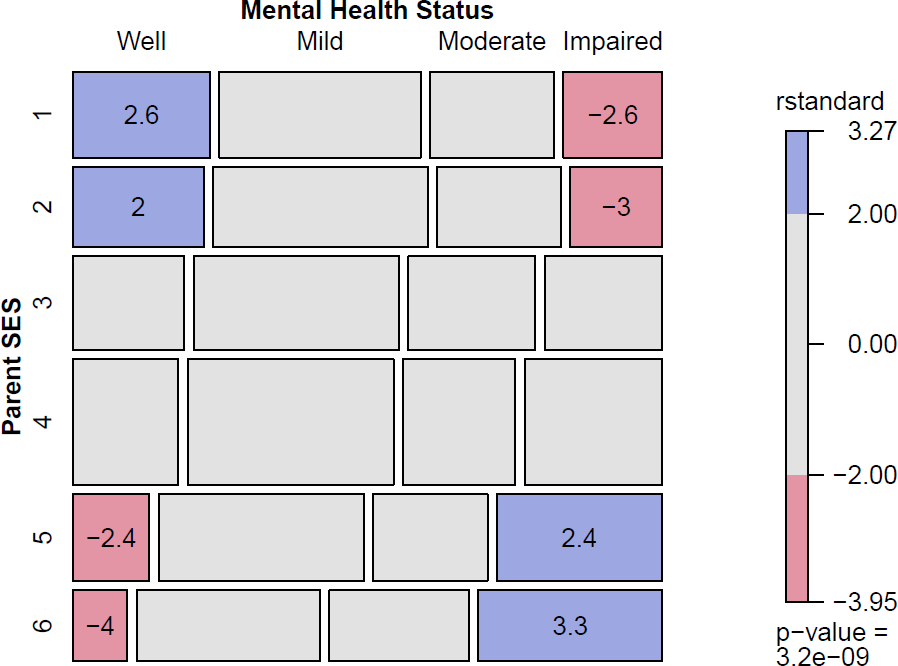
\includegraphics[width=.8\textwidth]{front/fig/mental-plot1} 
% \\
% 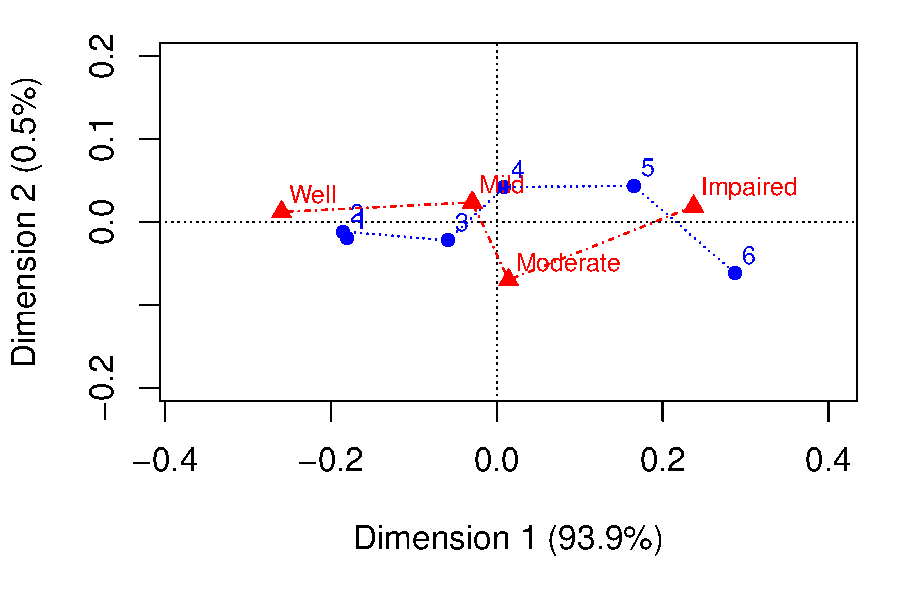
\includegraphics[width=.8\textwidth]{ch06/fig/ca-mental-plot}
}
%\end{titlepage}
\maketitle

%\begin{titlepage}
\title{%
%% simple cover pic for now
\Huge{Visualizing Categorical Data with }

\includegraphics[height=2ex, keepaspectratio]{front/fig/Rlogo}
% below-- use a graphic coverpage
%\input{front/covnew}
%\input{front/covpic}
}
\author{
	{\Large Michael Friendly} \\ York University
	\and
	{\Large David Meyer} \\ UAS Technikum Wien
%	\and
%	with contributions, \\ {\Large Achim Zeilleis} \\ Universit\"at Insbruck
}
\date{\today}
\vspace{1cm}
\titlepic{%
 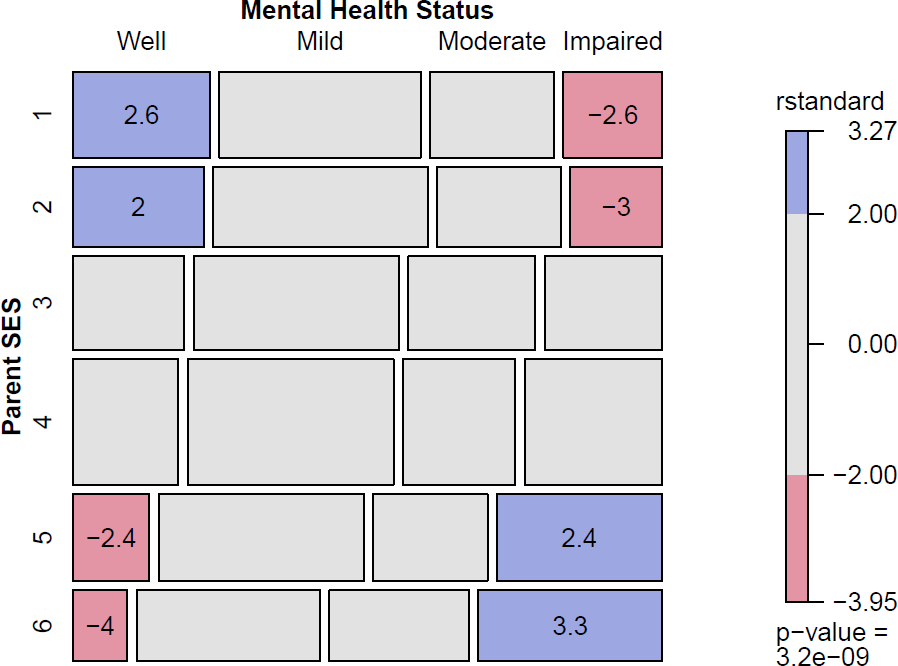
\includegraphics[width=.8\textwidth]{front/fig/mental-plot1} 
% \\
% 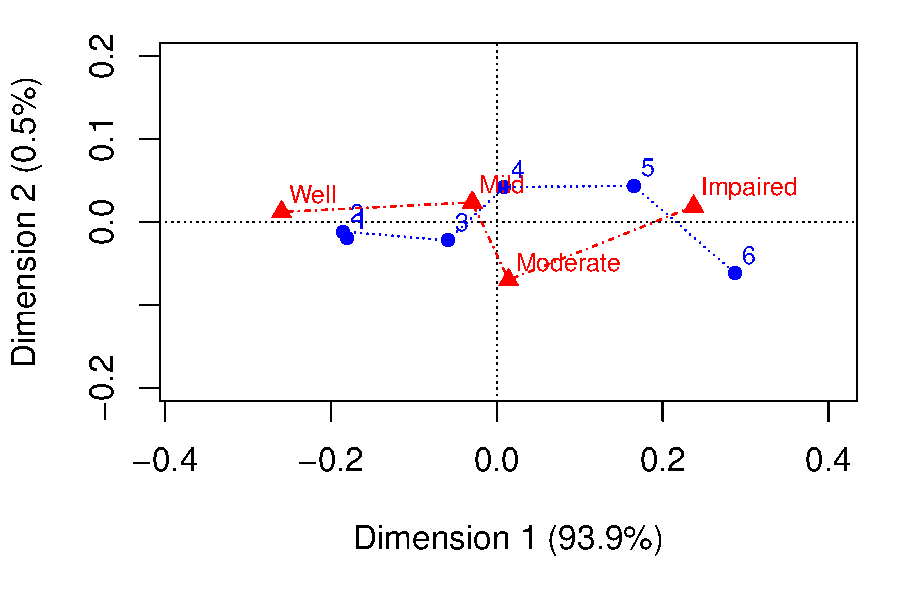
\includegraphics[width=.8\textwidth]{ch06/fig/ca-mental-plot}
}
%\end{titlepage}
\maketitle

\pagenumbering{roman}

%\addcontentsline{toc}{section}{Table of Contents}
{\renewcommand{\baselinestretch}{.8}\normalsize
\tableofcontents
}
%
%{\renewcommand{\baselinestretch}{.75}\normalsize
%\addcontentsline{toc}{section}{List of Tables}
%\listoftables
%}
%%
%{\renewcommand{\baselinestretch}{.75}\normalsize
%\addcontentsline{toc}{section}{List of Figures}
%\listoffigures
%}
%
%{\renewcommand{\baselinestretch}{.75}\normalsize
%\addcontentsline{toc}{section}{List of Outputs}
%\listof{Output}{List of Outputs}
%}
%
%\addtocontents{toc}{\protect\addcontentsline{toc}{section}{Table of Contents}}

\chapter{Preface}
%\addcontentsline{toc}{chapter}{\numberline{}Preface}

\TODO{The preface has not yet been written.  This is just a stub.}

\section*{Audience}
% This book assumes basic understanding of statistical concepts at least at an
% intermediate undergraduate level including regression and analysis of variance
% (for example, at the level of \citet{Neter-etal:90,MendenhallSincich:2003}).
% 
% It is written to appeal to two audiences:
% \begin{itemize*}
%   \item Students and methodologists in the social and health sciences, epidemiology,
%     economics, business
% 	and (bio)statistics
% 	\item Substantive researchers in various disciplines wanting to be able to
% 	apply these methods to their own data
% \end{itemize*}
% 
% It is also assumed that the reader has at least basic knowledge of the \R language and
% environment, including interacting with the \R console (RGui for Windows, R.app for Mac OS X)
% or other graphical user interface (e.g., R Studio), using \R functions in packages,
% getting help for these from \R, etc.  One introductory chapter (\chref{ch:working}) is devoted
% to covering topics beyond such basic skills needed in the book.

\section*{Overview}

\section*{Acknowledgements}


%% ============ Main matter ================
\mainmatter
\pagenumbering{arabic}
\chapter{Basic Concepts}

A component part for an electronic item is
manufactured at one of three different factories, and then delivered to
the main assembly line.Of the total number supplied, factory A supplies
50\%, factory B 30\%, and factory C 20\%. Of the components
manufactured at factory A, 1\% are faulty and the corresponding
proportions for factories B and C are 4\% and 2\% respectively. A
component is picked at random from the assembly line. What is the
probability that it is faulty? 

\section{Introduction}\label{intro}
The term reliability usually refers to the probability that a
component or system will operate satisfactorily either at any particular
instant at which it is required or for a certain length of
time. Fundamental to quantifying reliability s a knowledge of how to
define, assess and combine probabilities \cite{Bontempi2005Adaptive}. This may hinge on identifying the
form of the variability which is nherent n most processes. If all
components had a fixed known lifetime there would be no need to model
reliability.

\begin{enumerate}[1.]
\item A component part for an electronic item is
manufactured at one of three different factories.

\item A component part $x$ for an electronic item is
manufactured at one of three different factories.
\begin{enumerate}
\item A component part for an electronic item is
manufactured at one of three different factories.

\item A component part $x$ for an electronic item is
manufactured at one of three different factories.
\begin{enumerate}[iv.]
\item A component part for an electronic item is
manufactured at one of three different factories.

\item A component part $x$ for an electronic item is
manufactured at one of three different factories.

\item A component part for an electronic item is
manufactured at one of three different factories.

\item A component part 1, 2, 3, 4 for an electronic item is
manufactured at one of three different factories.

\item A component part for enumerate list of an electronic item is
manufactured at one of three different factories.

\end{enumerate}

\item A component part for an electronic item is
manufactured at one of three different factories.

\item A component part 1, 2, 3, 4 for an electronic item is
manufactured at one of three different factories.

\item A component part for enumerate list of an electronic item is
manufactured at one of three different factories.

\end{enumerate}

\item A component part for an electronic item is
manufactured at one of three different factories.

\item A component part 1, 2, 3, 4 for an electronic item is
manufactured at one of three different factories.

\item A component part for enumerate list of an electronic item is
manufactured at one of three different factories.

\end{enumerate}

\subsection{A component part}
A component part for an electronic item is
manufactured at one of three different factories, and then delivered to
the main assembly line.Of the total number supplied, factory A supplies
50\%, factory B 30\%, and factory C 20\%. Of the components
manufactured at factory A, 1\% are faulty and the corresponding
proportions for factories B and C are 4\% and 2\% respectively. A
component is picked at random from the assembly line. What is the
probability that it is faulty \cite{ilyas2004hsn}? 
A component part for an electronic item is
manufactured at one of three different factories, and then delivered to
the main assembly line. Of the total number supplied, factory A supplies
50\%, factory B 30\%, and factory C 20\%. Of the components
manufactured at factory A, 1\% are faulty and the corresponding
proportions for factories B and C are 4\% and 2\% respectively. A
component is picked at random from the assembly line. What is the
probability that it is faulty? 
A component part for an electronic item is
manufactured at one of three different factories, and then delivered to
the main assembly line.Of the total number supplied, factory A supplies
50\%, factory B 30\%, and factory C 20\%. Of the components
manufactured at factory A, 1\% are faulty and the corresponding
proportions for factories B and C are 4\% and 2\% respectively. A
component is picked at random from the assembly line. What is the
probability that it is faulty? 

\begin{VF}
``A Process is a structured, measured set of activities designed to produce a specific output for a particular customer
or market---A process is thus a specific ordering of work activities across time and space, with a beginning, an end.
and clearly defined inputs and outputs: a structure for action.''

\VA{Thomas Davenport}{Senior Adjutant to the Junior Marketing VP}
\end{VF}


\begin{table}%1
%\noautomaticrules
\tabletitle{Now we are engaged $(a_g^a)$ $\big(a_g^a\big)$ in a great civil war, testing whether that
nation, or any nation so conceived.}%
\begin{tabular}{lccc}
\tch{Scene}    &\tch{Reg. fts.} &\tch{Hor. fts.} &\tch{Ver. fts.}\\
Ball &19, 221 &4, 598   &3, 200\\
Pepsi$^a$&46, 281 &6, 898 &5, 400\\
Keybrd$^b$   &27, 290 &2, 968 &3, 405\\
Pepsi    &14, 796 &9, 188 &3, 209\\
\end{tabular}
\end{table}

\textbf{MultiRelational $k$-Anonymity.} Most works on $k$-anonymity focus on anonymizing a single data table; however, a real-life \cite{diamantaras1996pcn} database usually contains multiple relational tables. This has proposed a privacy model called \emph{MultiR $k$-anonymity} to ensure $k$-anonymity on multiple relational tables. Their model assumes that a relational database contains a person-specific table $PT$ and a set of tables $T_1,\cdots,T_n$, where $PT$ contains a person identifier $Pid$ and some sensitive attributes, and $T_i$, for $1 \leq i \leq n$, contains some foreign keys, some attributes in $QID$, and sensitive attributes. The general privacy notion is to ensure that for each record owner $o$ contained in the join of all tables $PT \Join T_1 \Join \cdots \Join T_n$, there exists at least $k-1$ other record owners share the same $QID$ with $o$. It is important to emphasize that the $k$-anonymization is applied at the \emph{record owner} level, not at the \emph{record} level in traditional $k$-anonymity. This idea is similar to $(X,Y)$-anonymity, where $X=QID$ and $Y=\{Pid\}$.

Most works on $k$-anonymity focus on anonymizing a single data table; however, a real-life \cite{diamantaras1996pcn} database usually contains multiple relational tables. This has proposed a privacy model called \emph{MultiR $k$-anonymity} to ensure $k$-anonymity on multiple relational tables. Their model assumes that a relational database contains a person-specific table $PT$ and a set of tables $T_1,\cdots,T_n$, where $PT$ contains a person identifier $Pid$ and some sensitive attributes, and $T_i$, for $1 \leq i \leq n$, contains some foreign keys, some attributes in $QID$, and sensitive attributes. The general privacy notion is to ensure that for each record owner $o$ contained in the join of all tables $PT \Join T_1 \Join \cdots \Join T_n$, there exists at least $k-1$ other record owners share the same $QID$ with $o$. It is important to emphasize that the $k$-anonymization is applied at the \emph{record owner} level, not at the \emph{record} level in traditional $k$-anonymity. This idea is similar to $(X,Y)$-anonymity, where $X=QID$ and $Y=\{Pid\}$.

\begin{table}[b!]%2
\tabletitle[Short Table Caption]{Now we are engaged $(a_g^a)$ $\big(a_g^a\big)$ in a great civil war, testing whether that
nation, or any nation so conceived.}%}{%
\begin{tabular}{lccc}
\tch{Scene}    &\tch{Reg. fts.} &\tch{Hor. fts.} &\tch{Ver. fts.}\\
\multicolumn{4}{@{}l@{}}{\tsh{Table Head}}\\[3pt]\hline\\[-6pt]
Ball &19, 221 &4, 598   &3, 200\\
Pepsi &46, 281 &6, 898 &5, 400\\
Keybrd   &27, 290 &2, 968 &3, 405\\
Pepsi    &14, 796 &9, 188 &3, 209\\
\end{tabular}
\end{table}

\begin{shadebox}
A component part for an electronic item is
manufactured at one of three different factories, and then delivered to
the main assembly line.Of the total number supplied, factory A supplies
50\%, factory B 30\%, and factory C 20\%. Of the components
manufactured at factory A, 1\% are faulty and the corresponding
proportions for factories B and C are 4\% and 2\% respectively. A
component is picked at random from the assembly line. What is the
probability that it is faulty? 
\end{shadebox}

In most literature on PPDP, they \cite{jolliffe2002pca} consider a more relaxed, yet more practical, notion of privacy protection by assuming limited attacker's background knowledge. Below, the term ``victim" refers to the record owner being linked. We can broadly classify linking models to two families.

\begin{extract}
A component part for an electronic item is \cite{hyvarinen2001ica}
manufactured at one of three different factories, and then delivered to
the main assembly line.Of the total number supplied, factory A supplies
50\%, factory B 30\%, and factory C 20\%. Of the components
manufactured at factory A, 1\% are faulty and the corresponding
proportions for factories B and C are 4\% and 2\% respectively. 
\end{extract}


One family considers a privacy threat occurs when an attacker is able to link a record owner to a record in a published data table, to a sensitive attribute in a published data table, or to the published data table itself. We call them \emph{record linkage}, \emph{attribute linkage}, and \emph{table linkage}, respectively. In all types of linkages, we assume that the attacker knows the $QID$ of the victim. In record and attribute linkages, we further assume that the attacker knows the presence of the victim's record in the released table, and seeks to identify the victim's record and/or sensitive information from the table \cite{yao2002can}. In table linkage, the attack seeks to determine the present or absent of the victim's record in the released table. A data table is considered to privacy preserved if the table can effectively prevent the attacker from successfully performing these types of linkages on the table \cite{madden2002tta}. Sections~\ref{intro}-\ref{sec:reclinkage} study this family of privacy models.
\begin{equation}
\mbox{var}\widehat{\Delta} = \sum_{j = 1}^t \sum_{k = j+1}^t
\mbox{var}\,(\hat{\alpha}_j - \hat{\alpha}_k)  = \sum_{j = 1}^t
\sum_{k = j+1}^t \sigma^2(1/n_j + 1/n_k). \label{2delvart2}
\end{equation}


An obvious measure of imbalance is just the difference in the
number of times the two treatments are allocated
\begin{equation}
D_n = \mathcal{M}|n_A - n_B|. \label{2deffD}
\end{equation}
For rules such as deterministic allocation, for which the expected
value of this difference can be calculated, we obtain the population
value ${\cal D}_n$.

\begin{shortbox}
\Boxhead{Box Title Here}
Another family aims at achieving the \emph{uninformative principle}: The published table should provide the attacker with little additional information beyond the background knowledge. There should not be a large difference between the prior and posterior beliefs; otherwise, there is a privacy threat~\cite{jain2004ass, jolliffe2002pca}. Many privacy models in this family are designed for statistical database and do not distinguish attributes in $T$ into $QID$, but some of them could also thwart record, attribute, and table linkages. Section~\ref{intro} studies this family of privacy models.

Let $m$ be a prime number. With the addition and multiplication as 
defined above, $Z_m$ is a field.
\end{shortbox}

\begin{theorem}\label{1th:Z_m}
Let $m$ be a prime number. With the addition and multiplication as 
defined above, $Z_m$ is a field.
\end{theorem}

\begin{proof}
Most of the proof of this theorem is routine.  It is clear that $0\in Z_m$ 
and $1\in Z_m$ are the 
zero element and identity element. If $a\in Z_m$ and $a\ne 0$, then $m-a$ 
is the additive inverse of $a$. If $a\in Z_m$ and $a\ne 0$, then the 
greatest common divisor of $a$ and $m$ is 1, and hence
there exist integers $s$ and $t$ such that $sa+tm=1$. Thus $sa=1 -tm$ is 
congruent to 1 modulo $m$. Let $s^*$ be the integer in $Z_m$ 
congruent to $s$ 
modulo $m$. Then we also have $s^*a\equiv 1\  \mbox{mod}\ m$. Hence $s^*$ 
is 
the multiplicative inverse of $a$ modulo $m$. Verification of the rest of 
the field properties is now routine.\end{proof}



\section{Record Linkage Model}\label{sec:reclinkage}

In the privacy attack of \emph{record linkage}, some value $qid$ on $QID$ identifies a small number of records in the released table $T$,
called a \emph{group}. If the victim's $QID$ matches the value
$qid$, the victim is vulnerable to being linked to the small
number of records in the group \cite{madden2005taq}. In this case, the attacker faces
only a small number of possibilities for the victim's record, and
with the help of additional knowledge, there is a chance that the
attacker could uniquely identify the victim's record from the
group.


%%%\begin{table}
%%%    \tabletitle{Examples for illustrating attacks}
%%%    \begin{tabular}{|c|c|c|c|}
%%%        \hline
%%%        \textbf{Job} & \textbf{Sex} & \textbf{Age} & \textbf{Disease} \\
%%%        \hline
%%%        Engineer & Male & 35 & Hepatitis \\
%%%        Engineer & Male & 38 & Hepatitis \\
%%%        Lawyer & Male & 38 & HIV \\
%%%        Writer & Female & 30 & Flu \\
%%%        Writer & Female & 30 & HIV \\
%%%        Dancer & Female & 30 & HIV \\
%%%        Dancer & Female & 30 & HIV \\
%%%        \hline
%%%    \end{tabular}
%%%    \label{table:rawpatient}
%%%\end{table}



\subsection{A component part}
A component part for an electronic item is
manufactured at one of three different factories, and then delivered to
the main assembly line.Of the total number supplied, factory A supplies
50\%, factory B 30\%, and factory C 20\%. Of the components
manufactured at factory A, 1\% are faulty and the corresponding
proportions for factories B and C are 4\% and 2\% respectively. A
component is picked at random from the assembly line. What is the
probability that it is faulty? 



\begin{figure}
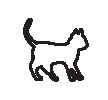
\includegraphics[width=350pt, height=200pt]{Chapters/chapter1/figures/cat.eps}
%%\centerline{\epsfig{/Chapters/chapter1/figures/cat.eps,width=.8\textheight,height=.4\textwidth}}
\caption[List of figure caption goes here]{Figure caption goes here.}
\end{figure}



\begin{figure}[htb]
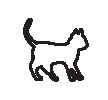
\includegraphics[width=200pt, height=200pt]{Chapters/chapter1/figures/cat.eps}
%%\centerline{\epsfig{figure=cat.eps,width=.5\textheight,height=.4\textwidth}}
\caption[Short figure caption]{Figure caption goes here. Figure caption goes here.
Figure caption goes here. Figure caption goes here. Figure caption goes here.
Figure caption goes here.}
\end{figure}





\begin{figure}
\begin{center}
\subfigure[\label{f8a}]{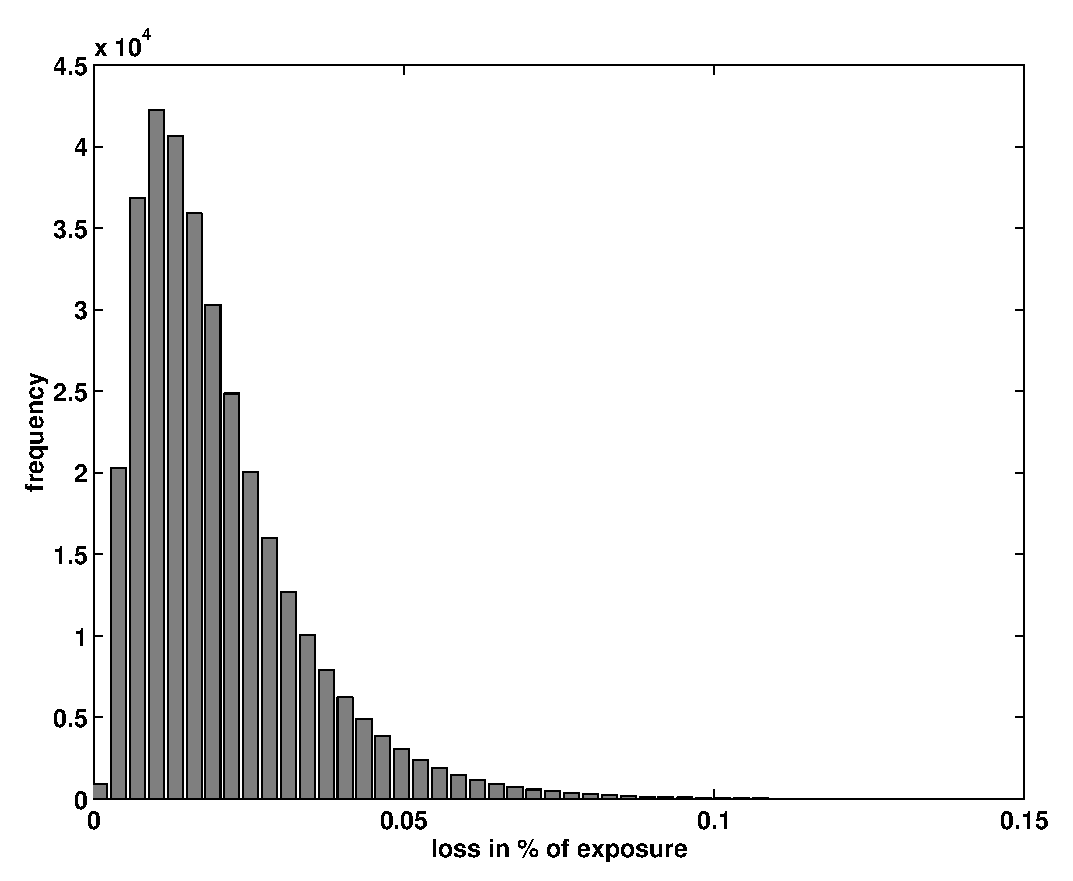
\includegraphics[angle=90,width=7cm,height=7cm,angle=-90]{Chapters/chapter1/figures/Histogram.eps}}
\subfigure[\label{f8b}]{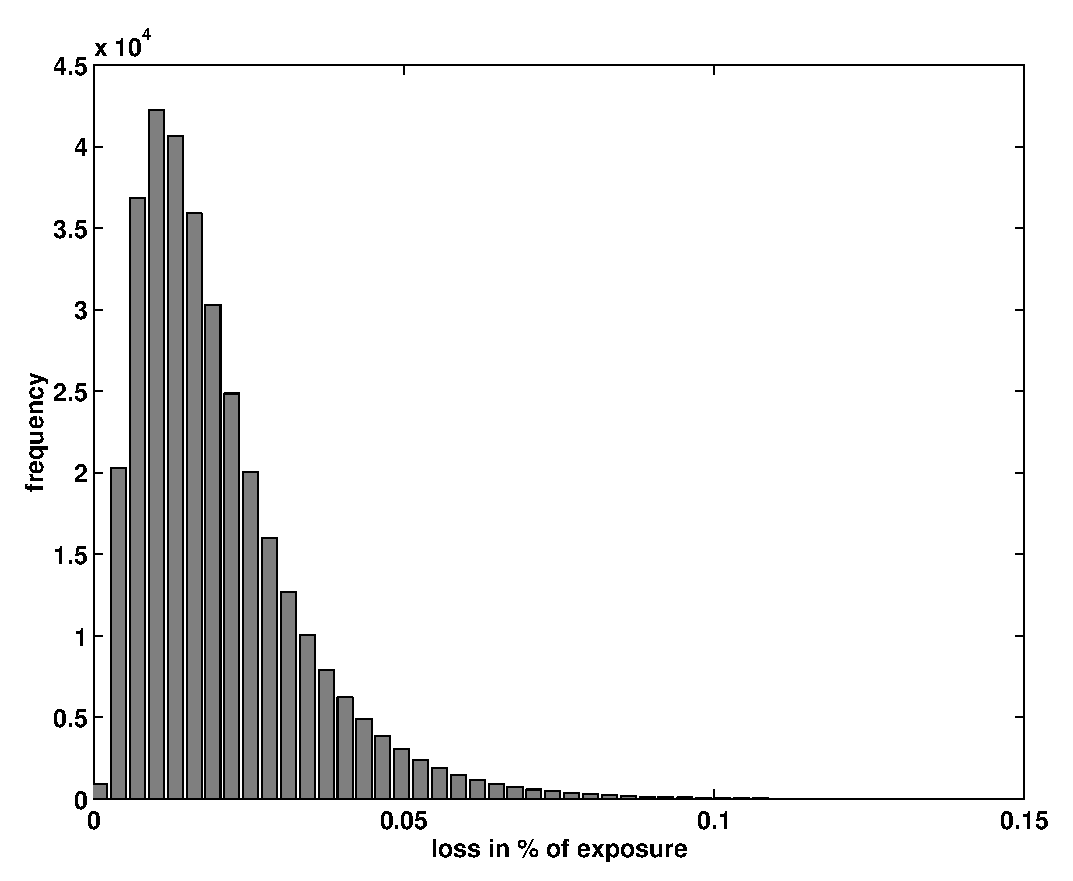
\includegraphics[angle=90,width=7cm,height=7cm,angle=-90]{Chapters/chapter1/figures/Histogram.eps}}
\end{center}
\caption[The bar charts depict the different risk contributions]{The bar charts depict the different risk contributions (top: 99\% quantile, bottom: 99.9\% quantile) of the business areas of a bank. The black bars
are based on a Var/Covar approach, the white ones correspond to shortfall risk.}
\end{figure}

\subsubsection{H3 A component part }
A component part for an electronic item is
manufactured at one of three \cite{mardia1979ma} different factories, and then delivered to
the main assembly line.Of the total number supplied, factory A supplies
50\%, factory B 30\%, and factory C 20\%. Of the components
manufactured at factory A, 1\% are faulty and the corresponding
proportions for factories B and C are 4\% and 2\% respectively. A
component is picked at random from the assembly line. What is the
probability that it is faulty? 


A fundamental notion \cite{yao2002can} is that of a\index{subspace}\index{vector 
space!subspace of} subspace of $F^n$. Let $V$ be a nonempty subset of 
$F^n$. Then $V$ is a {\it subspace} of $F^n$ provided $V$ is closed 
under vector addition and scalar multiplication, that is, 
\begin{enumerate} 
\item[\rm (a)] For all $u$ and $v$ in $V$, $u+v$ is 
also in $V$. 
\item[\rm (b)] For all $u$ in $V$ and $c$ in $F$, $cu$ is 
in $V$. 
\end{enumerate} 
Let $u$ be in the subspace $V$. Because $0u=0$, 
it follows that the zero vector is in $V$. Similarly, $-u$ is in $V$ 
for all $u$ in $V$. A simple example of a subspace of $F^n$ is the set 
of all vectors $(0,a_2,\ldots,a_n)$ with first coordinate equal to 0. 
The zero vector itself is a subspace.

\begin{definition}\label{1def:linearcomb}{\rm
Let $u^{(1)},u^{(2)},\ldots,u^{(m)}$ be vectors in $F^n$, and let 
$c_1,c_2,\ldots,c_m$ be scalars. Then the vector
\[c_1u^{(1)}+c_2u^{(2)}+\cdots+c_mu^{(m)}\]
is called a {\it linear combination} \index{linear combination} of $u^{(1)},u^{(2)},\ldots,u^{(m)}$.
If $V$ is a subspace of $F^n$, then $V$ is closed under vector addition and 
scalar multiplication, and it follows easily by induction that a 
linear combination of vectors in $V$ is also a vector in $V$. Thus 
{\it subspaces 
are closed under linear combinations}; in fact, this can be taken as the 
defining property of subspaces.
The vectors $u^{(1)},u^{(2)},\ldots,u^{(m)}$ {\it span} $V$ \index{spanning set}
(equivalently, form a {\it spanning set} of $V$) provided every vector in 
$V$ 
is a linear combination of $u^{(1)},u^{(2)},\ldots,u^{(m)}$. The zero 
vector can be written as a linear combination of 
$u^{(1)},u^{(2)},\ldots,u^{(m)}$ with all scalars equal to 0; this is a 
{\it trivial linear combination}.\index{linear combination!trivial} The vectors
$u^{(1)},u^{(2)},\ldots,u^{(m)}$ are {\it linearly dependent} provided 
there are scalars $c_1,c_2,\ldots,c_m$, not all of which are zero, such 
that
\[c_1u^{(1)}+c_2u^{(2)}+\cdots+c_mu^{(m)}=0,\]
that is, the zero vector can be written as a {\it nontrivial linear \index{linear combination!nontrivial} 
combination} of $u^{(1)},u^{(2)},\ldots,u^{(m)}$.
For example, the vectors $(1,4), (3,-1)$, and $(3,5)$ in $\Re^2$ are 
linearly 
dependent since
\[3(1,4)+1(3,-2)-2(3,5)=(0,0).\] Vectors are {\it linearly independent} provided  they are not linearly dependent.\index{linearly independent}
The vectors 
$u^{(1)},u^{(2)},\ldots,u^{(m)}$ are a {\it basis} \index{basis} of $V$ provided they are  
linearly independent and span $V$.
By an {\it ordered basis} \index{basis!ordered} we mean a basis in which the vectors of the basis are listed 
in a specified order; to indicate that we have an ordered basis we write
$(u^{(1)},u^{(2)},\ldots,u^{(m)})$. 
A spanning set $S$ of $V$ is a \index{spanning set!minimal} {\it minimal spanning set of $V$} provided that
each set 
of vectors obtained from $S$ by removing a vector is not a spanning set 
for $V$.
A linearly independent set $S$ of vectors of $V$ is a {\it maximal linearly \index{linearly independent!maximal}
independent set of vectors of $V$} provided that for each vector $w$ of 
$V$ that 
is not in $S$, $S\cup\{w\}$ is  linearly dependent (when this happens, 
$w$ must be  a linear combination of the vectors in 
$S$).\hfill{$\Box$}
}\end{definition}

In addition to matrix addition, subtraction, and multiplication, there is 
one additional operation that we define now. It's perhaps the simplest of 
them all. Let $A=[a_{ij}]$ be an $m$ by $n$ matrix and let $c$ be a 
number \cite{hyvarinen2001ica}. Then the matrix $c\cdot A$, or simply $cA$, is the $m$ by $n$ 
matrix obtained by multiplying each entry of $A$ by $c$:
\[c A=[ca_{ij}].\]\index{matrix!scalar multiplication} \index{matrix!scalar multiple of}
The matrix $c A$ is called a {\it scalar multiple} of $A$.

\begin{VT1}

\VH{Think About It...}

Commonly thought of as the first modern computer, ENTAC was built in 1944. It took up more space than an 18-wheeler's
tractor trailer and weighed more than 17 Chevrolet Camaros. It consumed 140,000 watts of electricity while executing
up to 5,000 basic arithmetic operations per second. One of today's popular microprocessors, the 486, is built on a
tiny piece of silicon about the size of a dime.

\VT
With the continual expansion of capabilities, computing power will eventually exceed the capacity for human
comprehension or human control.

\VTA{The Information Revolution}{Business Week}
\end{VT1}


\section{Glossary}
\begin{Glossary}
\item[360 Degree Review] Performance review that includes feedback from superiors, peers, subordinates, and clients.
\item[Abnormal Variation] Changes in process performance that cannot be accounted for by typical day-to-day variation. Also referred to as
non-random variation.
\item[Acceptable Quality Level (AQL)] The minimum number of parts that must comply with quality standards, usually stated as a percentage.
\item[Activity] The tasks performed to change inputs into outputs.
\item[Adaptable] An adaptable process is designed to maintain effectiveness and efficiency as requirements change. The process is
deemed adaptable when there is agreement among suppliers, owners, and customers that the process will meet
requirements throughout the strategic period.
\end{Glossary}




\chapter{Fitting and graphing discrete distributions}\label{ch:discrete}
\begin{center}
 \rule[-4pt]{0.5pt}{4pt}\hrulefill\rule[-4pt]{0.5pt}{4pt}\\
 \begin{minipage}[c]{.33\linewidth}
  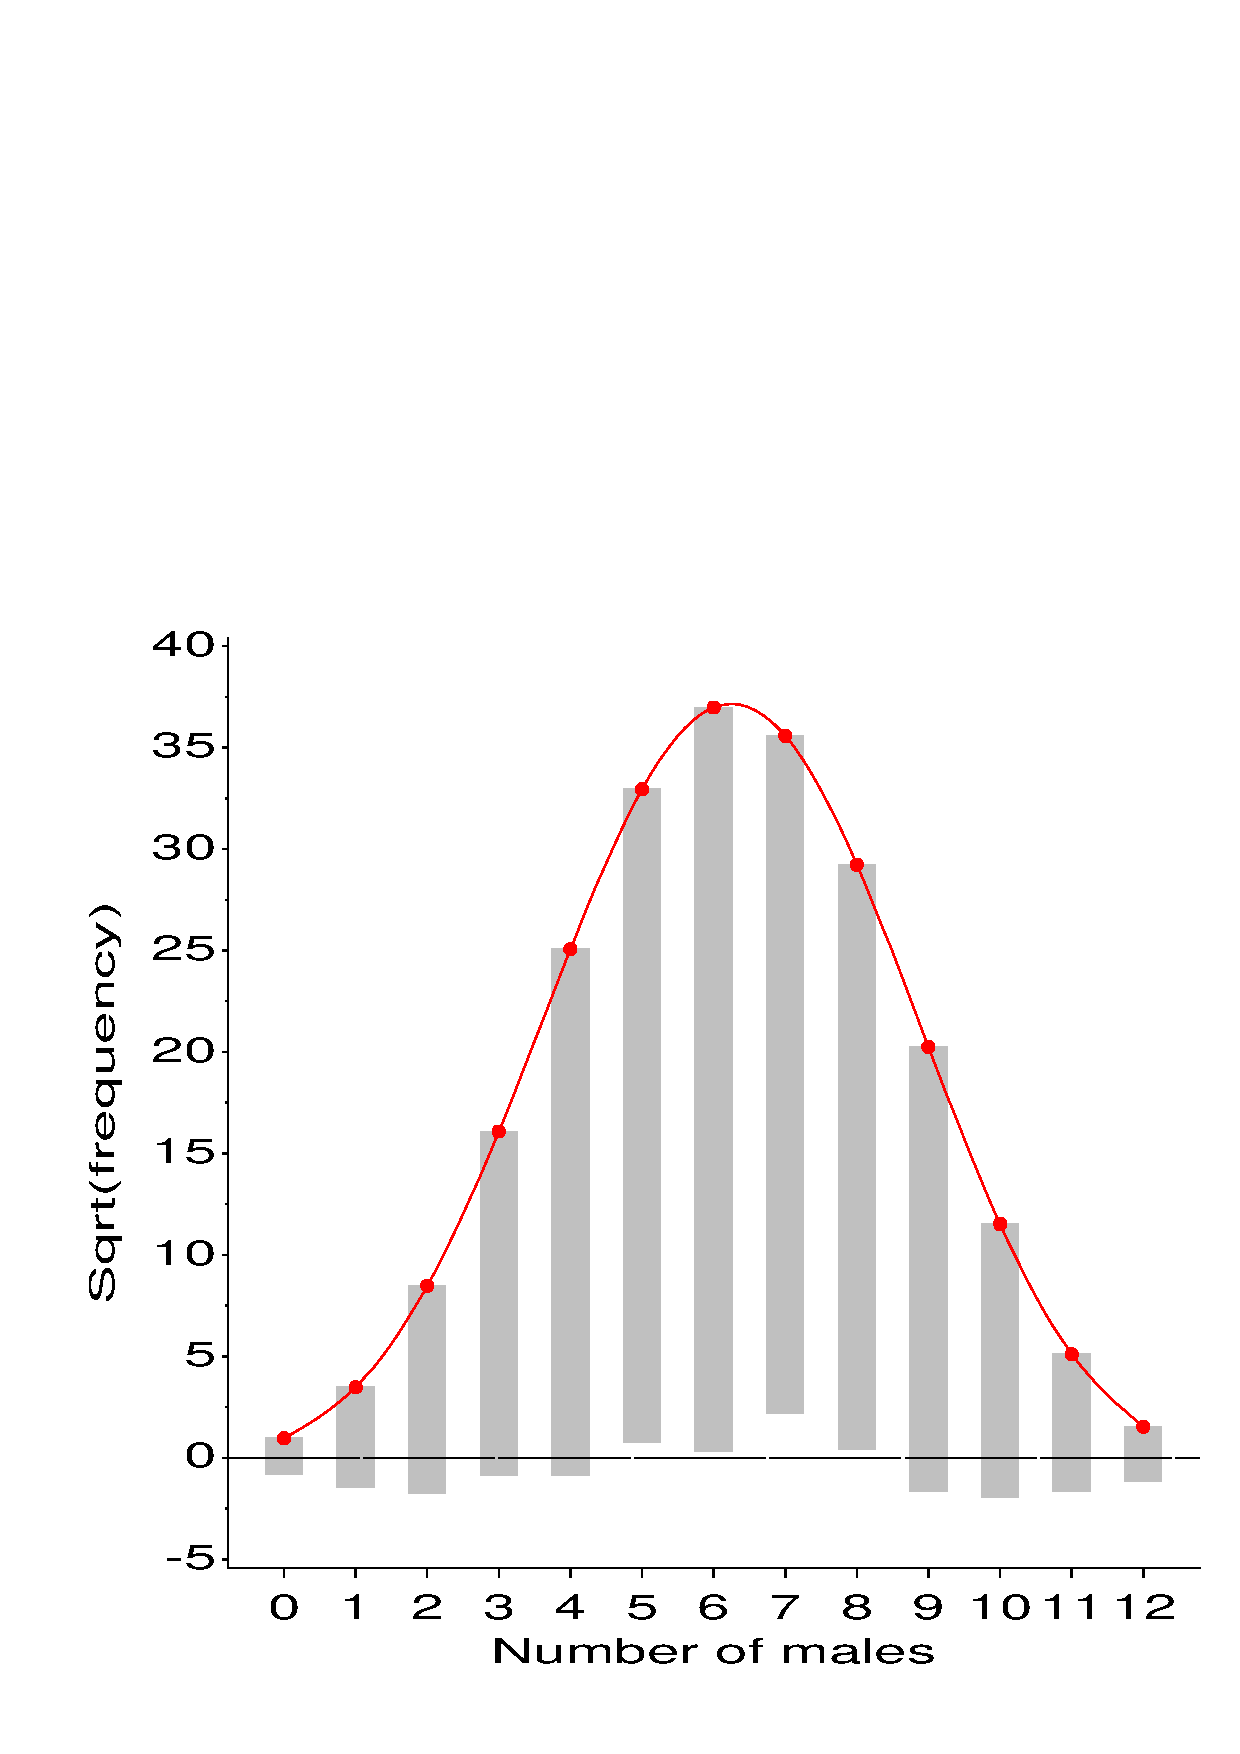
\includegraphics[width=1\linewidth]{saxony}\graphicsfile{ch2/fig/saxony.eps}{}
 \end{minipage}%
 \hfill
 \begin{minipage}[c]{.33\linewidth}
  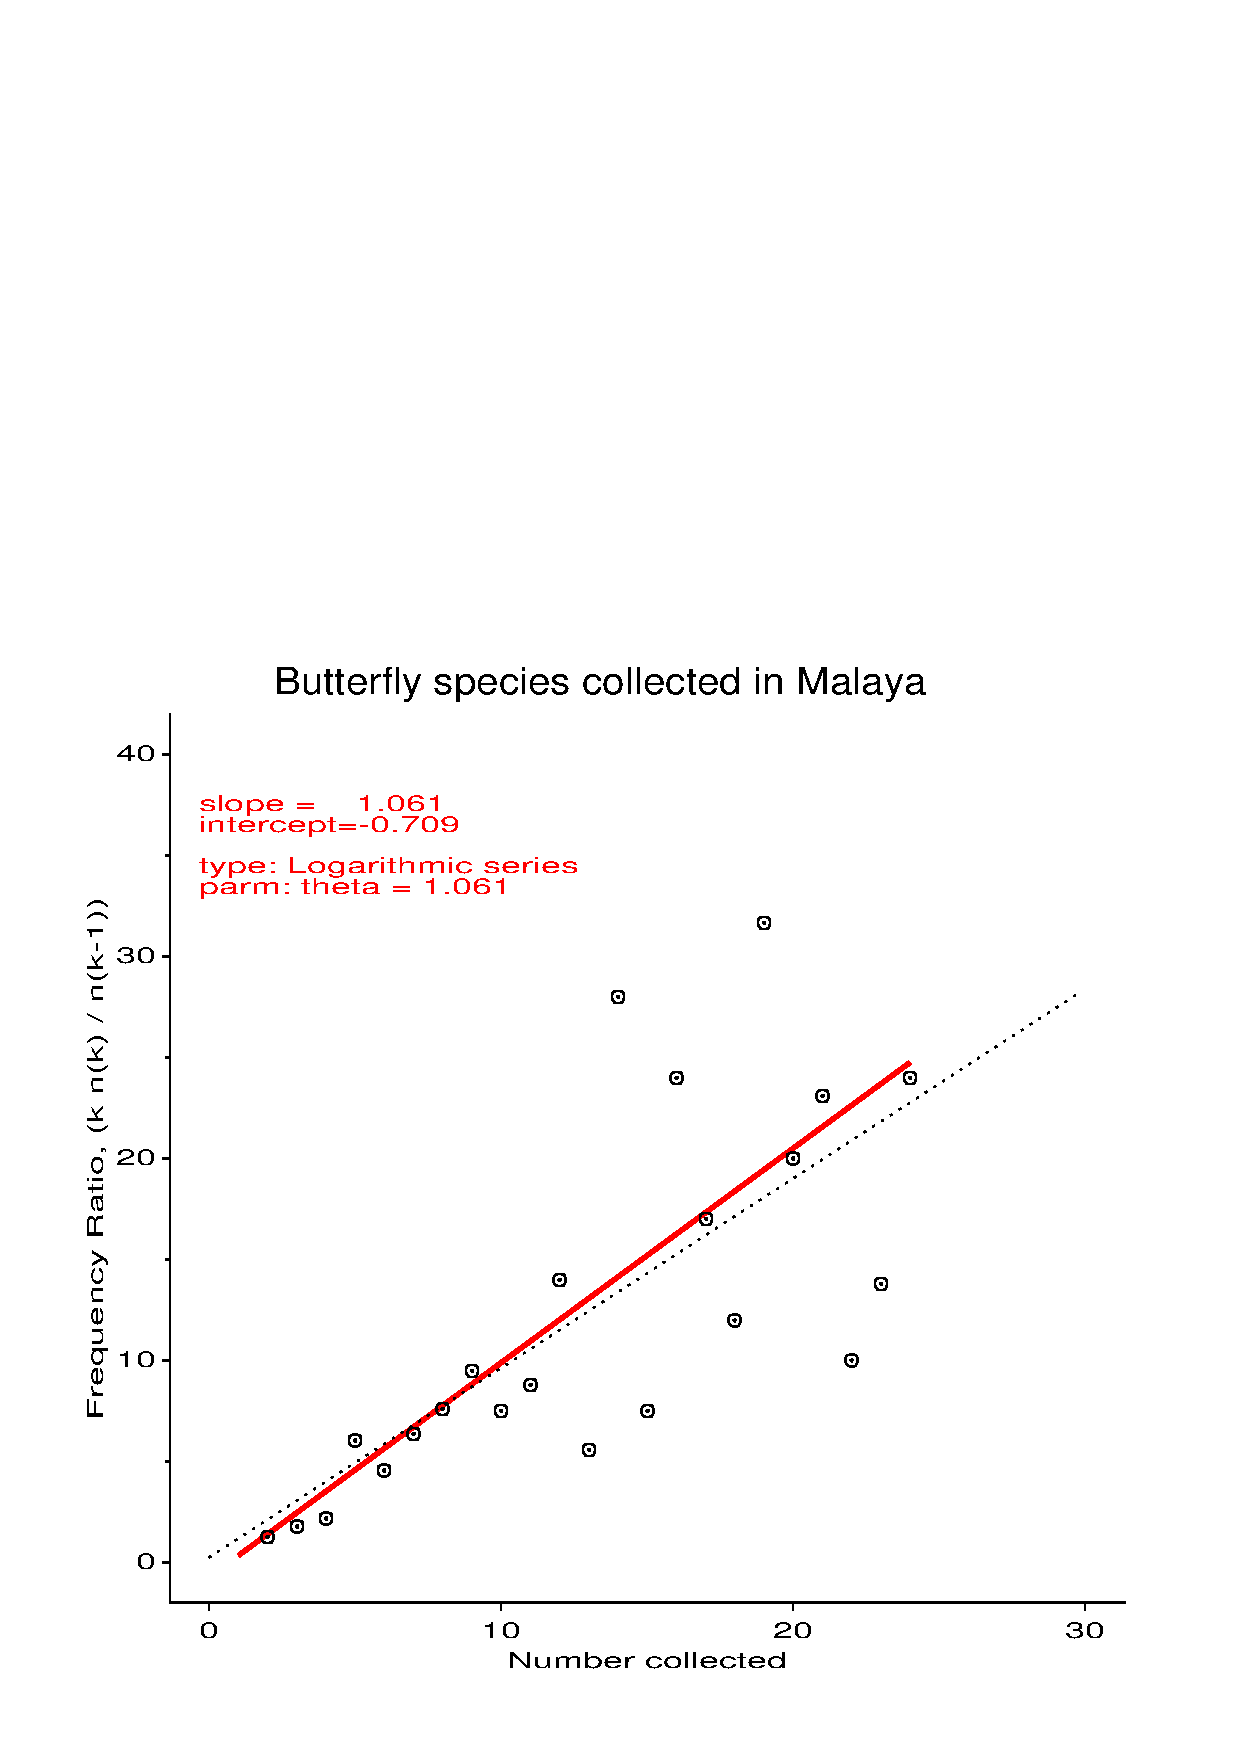
\includegraphics[width=1\linewidth]{orddemo3}\graphicsfile{ch2/fig/orddemo3.eps}{}
 \end{minipage}
 \hfill
 \begin{minipage}[c]{.33\linewidth}
  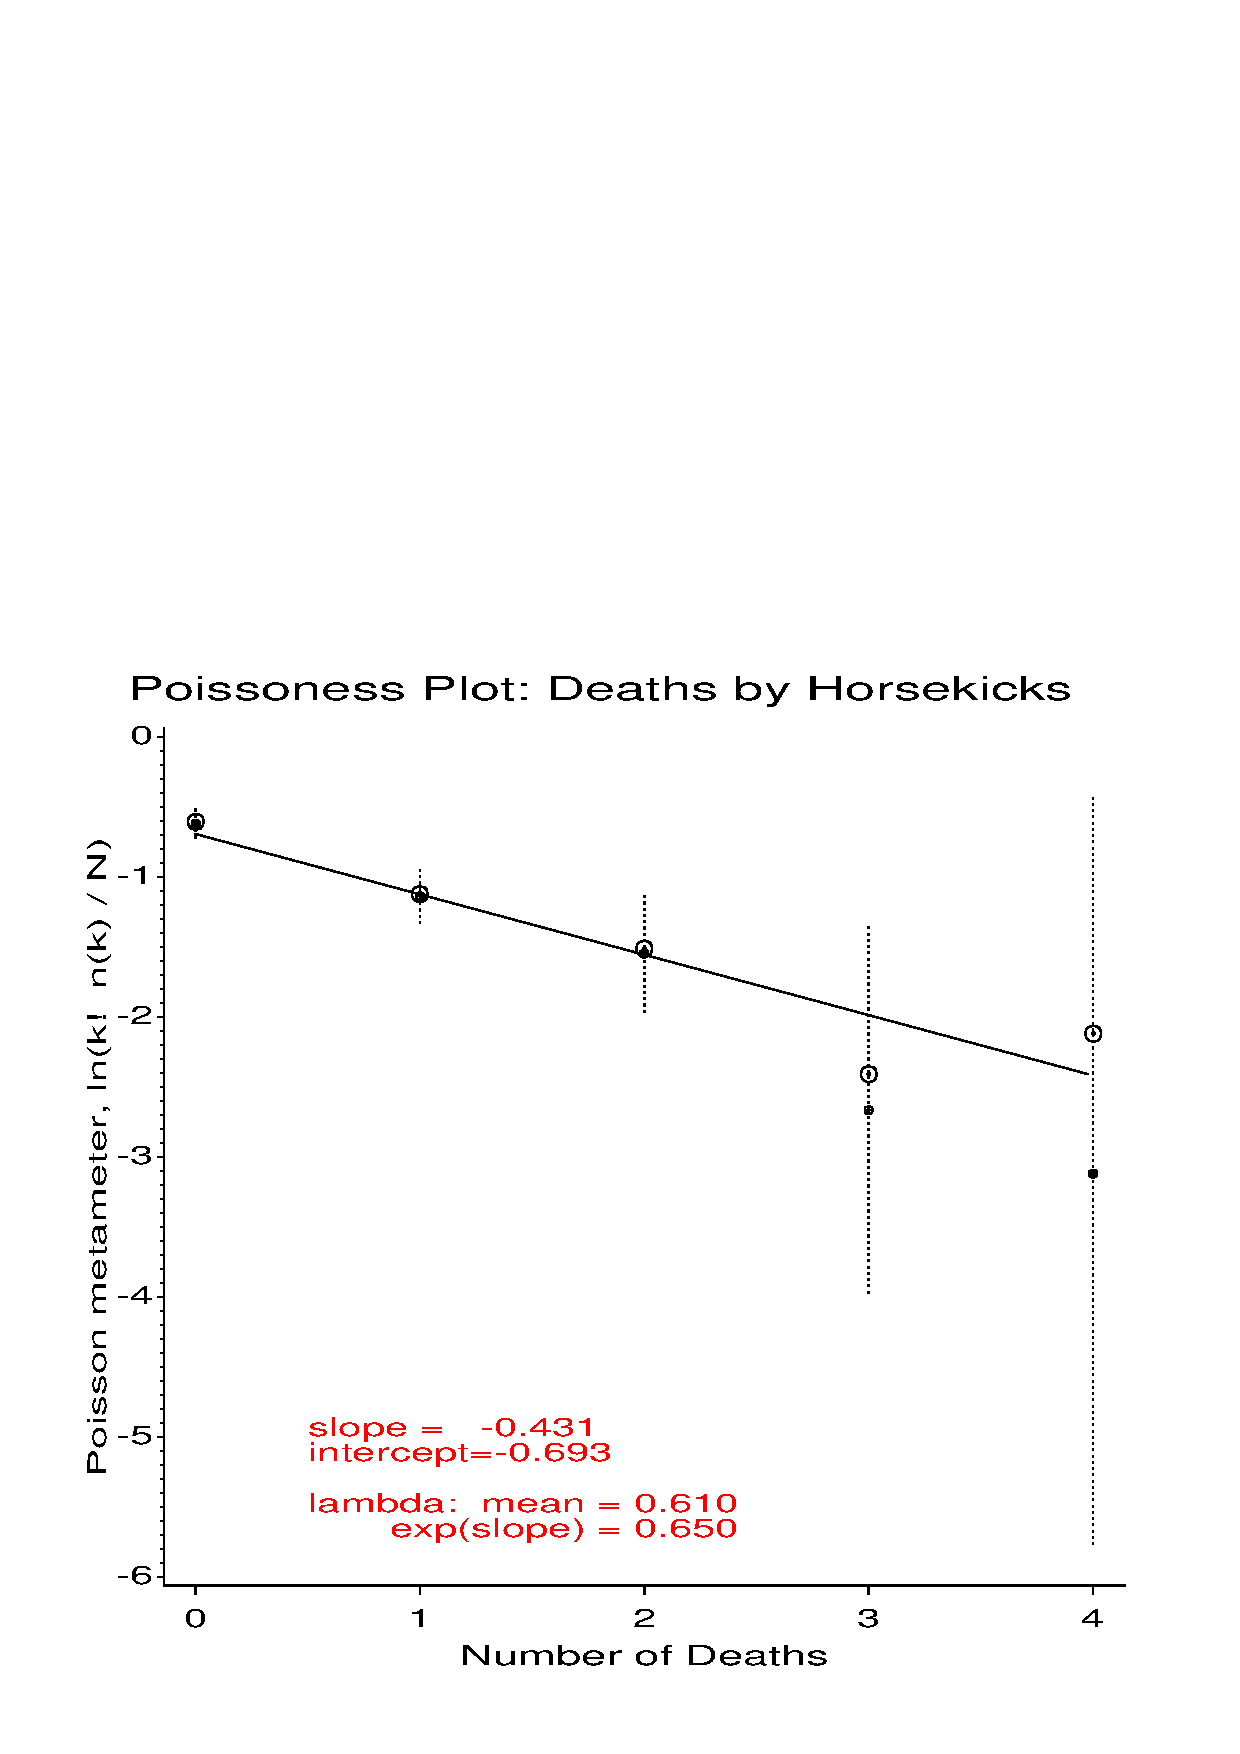
\includegraphics[width=1\linewidth]{poisdemo1}\graphicsfile{ch2/fig/poisdemo1.eps}{}
 \end{minipage}
\end{center}


\begin{quote}
{\Large
Discrete data often follow various theoretical probability models.
Graphic displays are used to visualize goodness of fit,
to diagnose an appropriate model, and determine the impact of
individual observations on estimated parameters.
}
\end{quote}
\minitoc
\clearpage

\section{Introduction}
\epigraph{Not everything that counts can be counted, and not everything that
can be counted counts.}
{Albert Einstein}
Discrete frequency distributions often involve counts of occurrences
such as accident fatalities, words in passages of text,  births of twins,
events of terrorism or suicide, or blood
cells with some characteristic.  Typically such data consist of a
table which records that \(n_k\) of the observations pertain to the
basic outcome value \(k \,  , \,  k = 0 , 1, \dots\).
For such data, we often wish to understand the process which gives rise to
these numbers, or to estimate frequencies for outcome values $k$ we
did not observe.  Both goals can be approached by examining
how closely the data follow a particular discrete probability distribution, such as the Poisson, the binomial, or the geometric distribution.

We briefly describe the properties of some of the most widely used
discrete distributions in \secref{sec:discrete-distrib}, along with
SAS techniques for calculating and visualizing those distributions.
\secref{sec:discrete-fit} presents theory and visualization techniques
related to fitting these distributions to empirical data.
In some cases, we may not know \emph{which} discrete distribution
should be fit to a given \Dset;  \secref{sec:discrete-Ord}
describes a simple graphical method designed to determine an appropriate
distribution type.
A more robust graphical method for diagnosing whether a given data
set follows the Poisson distribution is illustrated in \secref{sec:discrete-Poissonness}.
It turns out that the the discrete distributions described here
are members of a more general, parametric family, the \emph{power series},
permitting these
techniques to be applied to all of them.
A number of SAS macros to simplify the fitting and graphing of discrete
distributions are presented throughout the chapter.
  
The tables described in \exref{ex:horskick1}--\exref{ex:butterfly} illustrate several discrete data sets. For data such as these,
we can fit various discrete distributions and test hypotheses that
the fit is reasonably close.
However, rather than simply summarizing the goodness-of-fit in a
single number, we learn more from well-chosen graphical displays.

\begin{Example}[horskick1]{Death by horse kick}
One of the oldest and best known examples of a Poisson distribution
is the data from
\citet{Bortkiewicz:98} on deaths of soldiers in the Prussian
army from kicks by horses and mules, shown in \tabref{tab:horskick}.
von Bortkiewicz tabulated the number of soldiers in each of
14 army corps in the 20 years from 1875-1894
who died after being kicked by a horse
\citep[p. 18]{AndrewsHerzberg:85}.
\tabref{tab:horskick} shows the data used by
\citet{Fisher:25} for 10 of these
army corps, summed over 20 years, giving 200
`corps-year' observations.  In 109 corps-years,
no deaths occurred; 65 corps-years had one death, etc.
The data set is given more fully in \datref{dat:vonbort}.
The distribution is plotted in \figref{fig:poischart1}.
%% table from data set horskick (poistab.sas)
\begin{table}[htb]
\caption{Death by horse kicks}
\label{tab:horskick}
 \begin{center}
  \begin{tabular}{rr}
  \hline
Number of   & Number of  \\
Deaths ($k$)& Corps-Years ($n_k$)\\
  \hline
0 & 109 \\
1 & 65 \\
2 & 22 \\
3 & 3 \\
4 & 1 \\
  & N = 200 \\
  \hline
  \end{tabular}
 \end{center}
\end{table}

\end{Example}

\begin{Example}[madison1]{Federalist papers}
In 1787--88, Alexander Hamilton, John Jay, and James Madison
wrote a series of newspaper essays to persuade the voters of
New York State to ratify the U.S. Constitution.
The essays were titled \emph{The Federalist Papers}
and all were signed with the pseudonym ``Publius.''  Of the 77 papers published,
the author(s) of 65 are known, but \emph{both}
Hamilton and Madison later claimed sole authorship of the remaining 12.
\citet{MostellerWallace:84}
investigated the use of statistical methods to identify authors of
disputed works based on the frequency distributions of certain key
function words, and concluded that Madison had indeed authored the
12 disputed papers.  

\tabref{tab:madison} shows the distribution of the occurrence of one of
these ``marker'' words, 
the
word \emph{may} in 262 blocks of text (each about 200 words long)
from issues of the \emph{Federalist Papers} and other essays known
to be written by James Madison.  In 156 blocks, the word \emph{may}
did not occur; it occurred once in 63 blocks, etc.  The distribution
is plotted in \figref{fig:poischart2}.

%% table from data set madison (poistab.sas)
\begin{table}[htb]
\caption[Occurrences of `may' in Federalist Papers]{Number of Occurrences of the word \emph{may} in Federalist Papers
and essays written by James Madison}
\label{tab:madison}
 \begin{center}
  \begin{tabular}{rr}
  \hline
Number of        & Blocks of \\
Occurrences ($k$)& Text ($n_k$)\\
  \hline
0 & 156 \\
1 & 63 \\
2 & 29 \\
3 & 8 \\
4 & 4 \\
5 & 1 \\
6 & 1 \\
  & N = 262 \\
  \hline
  \end{tabular}
 \end{center}
\end{table}


\begin{figure}[htb]
 \begin{minipage}[b]{.5\linewidth}
  \centering
  \includegraphics[width=.9\linewidth,clip]{ch2/fig/poischart1.eps}
  \caption{von Bortkiewicz's data}\label{fig:poischart1}
 \end{minipage}%
 \begin{minipage}[b]{.5\linewidth}
  \centering
  \includegraphics[width=.9\linewidth,clip]{ch2/fig/poischart2.eps}
  \caption{Mosteller \& Wallace data}\label{fig:poischart2}
 \end{minipage}
\end{figure}

Note that the distributions of these data sets in \figref{fig:poischart1}
and \figref{fig:poischart2} are superficially similar in shape:
both have their mode at $k=0$ and frequencies $n_k$ which steadily
decline as $k$ increases.
Nevertheless, it turns out, the Horse Kick data is reasonably well-described by
a Poisson distribution, but the Madison data is not (Mosteller
and Wallace concluded that a negative binomial distribution provides
a better fit).
\end{Example}

Several other discrete distributions are illustrated by the
following examples.

\begin{Example}[queues]{Women in queues}
\citet{JinkinsonSlater:81,HoaglinTukey:85}
give the frequency distribution of the number of females observed in
queues of length 10 in a London Underground station.
If it is assumed that people line up independently, and that
men and women are equally likely to be found in a queue
(not necessarily reasonable assumptions),
then the number of women out of 10
would have a (symmetric) binomial distribution with parameters $N=10$ and
$p=\frac12$.
The frequency distribution, shown in \tabref{tab:queues},
appears systematically asymmetric, as we can see more clearly in
a histogram, \figref{fig:poischart3}.
However, there is no real reason to expect that males and females are
equally likely to be found in queues in the London underground,
so we may be interested in estimating $p$ from the data
and determining if a binomial distribution fits.

%% table from data set queues (poistab.sas) generated 16DEC97
\begin{table}[htb]
\caption{Number of women in 100 queues of length 10}
\label{tab:queues}
 \begin{center}
  \begin{tabular}{rr}
  \hline
Number of  & Number of \\
women ($k$) &  queues ($n_k$)\\
  \hline
0 & 1 \\
1 & 3 \\
2 & 4 \\
3 & 23 \\
4 & 25 \\
5 & 19 \\
6 & 18 \\
7 & 5 \\
8 & 1 \\
9 & 1 \\
10 & 0 \\
  & N=100 \\
  \hline
  \end{tabular}
 \end{center}
\end{table}


%% one figure
\begin{figure}[htb]
% \SASfig{poischart3.eps}{scale=.9}{poischart3}{Women in Queues of Length 10}
  \centering
  \includegraphics[scale=.9]{poischart3.eps}
  \caption{Women in Queues of Length 10}%
  \label{fig:poischart3}
\end{figure}
\end{Example}

\begin{Example}[dice]{Weldon's dice}
Common examples of binomial distributions involve tossing coins
or dice.
Perhaps the most industrious dice-tosser of all times,
Weldon tallied the results of throwing 12 dice 26,306 times
(a task which presumably required a good deal of leisure time).
He reported his results in a letter to Francis Galton dated
February 2, 1894, in order
``to judge whether the differences between a series of group frequencies
and a theoretical law \dots were more than might be attributed
to the chance fluctuations of random sampling''
\citep{KempKemp:91}.
In his seminal paper,
\citet{Pearson:00} used Weldon's data to illustrate the \chisq{} goodness-of-fit test, as did
\citet[Table 5.1, p. 121]{KendallStuart:63}.  These data are
shown here as
\tabref{tab:dice},
in terms of the number of occurrences of either a 5 or
6 in the throw of 12 dice.
If the dice were all identical and perfectly fair (balanced), one would
expect that $p = \Pr\{5 \textrm{ or } 6\} = \frac13$
and the distribution of the number of 5 or 6 would be binomial.
A peculiar feature of these data
as presented by Kendall and Stuart (not uncommon in discrete distributions)
is that the frequencies of 10--12 successes
are lumped together.  This grouping must be taken into account in fitting
the distribution.  The distribution is shown in \figref{fig:dice}.
%% table from data set dice (dice.sas) generated 26DEC97
\begin{table}[htb]
\caption{Frequencies of a 5 or 6 in throws of 12 dice}
\label{tab:dice}
 \begin{center}
  \begin{tabular}{rr}
  \hline
Number of  & Frequency \\
5s or 6s ($k$) & ($n_k$) \\
  \hline
0 & 185 \\
1 & 1149 \\
2 & 3265 \\
3 & 5475 \\
4 & 6114 \\
5 & 5194 \\
6 & 3067 \\
7 & 1331 \\
8 & 403 \\
9 & 105 \\
10+ & 18 \\
    & N=26306 \\
  \hline
  \end{tabular}
 \end{center}
\end{table}

%% one figure
\begin{figure}[htb]
%  \SASfig{dice.eps}{scale=.65}{dice}{Weldon's dice data}
  \centering
  \includegraphics[scale=.65]{dice.eps}
  \caption{Weldon's dice data}%
  \label{fig:dice}
\end{figure}
\end{Example}

\begin{Example}[butterfly]{Butterfly species in Malaya}
In studies of the diversity of animal species, individuals are
collected and classified by species.
The distribution of the number of species (types) where $k = 1, 2, \dots$
individuals (tokens) were collected forms a kind of type-token distribution.
An early example of this kind of distribution was presented by
\citet{Fisher-etal:43}.
\tabref{tab:butterfly} lists the number of individuals of each of
501 species of butterfly collected in Malaya.
There were thus 118 species for which just a single instance was found,
74 species for which two individuals were found,
down to 3 species for which 24 individuals were collected.
Fisher et-al.\  note however that the distribution was truncated
at $k = 24$.
Type-token distributions are often J-shaped, with a long upper tail,
as we see in \figref{fig:poischart4}.
%% table from data set butfly (poistab.sas) generated 11DEC97
\begin{table}[htb]
{
\small
\caption{Number of butterfly species for which $k$ individuals were collected}
\label{tab:butterfly}
 \begin{center}
  \begin{tabular}{rr|rr}
  \hline
Number of & Number of & Number of & Number of \\
Individuals ($k$)& Species ($n_k$) & Individuals ($k$)& Species ($n_k$)\\
  \hline
1 & 118 & 13 & 6 \\
2 & 74 & 14 & 12 \\
3 & 44 & 15 & 6 \\
4 & 24 & 16 & 9 \\
5 & 29 & 17 & 9 \\
6 & 22 & 18 & 6 \\
7 & 20 & 19 & 10 \\
8 & 19 & 20 & 10 \\
9 & 20 & 21 & 11 \\
10 & 15 & 22 & 5 \\
11 & 12 & 23 & 3 \\
12 & 14 & 24 & 3 \\
    & &   & N = 501 \\ 
  \hline
  \end{tabular}
 \end{center}
}
\end{table}


%% one figure
\begin{figure}[htb]
%  \SASfig{poischart4.eps}{width=.9\linewidth}{poischart4}{Butterfly species in Malaya}
  \centering
  \includegraphics[width=.9\linewidth]{poischart4.eps}
  \caption{Butterfly species in Malaya}%
  \label{fig:poischart4}
\end{figure}
\end{Example}

\section{Discrete distributions}\label{sec:discrete-distrib}
This section briefly reviews the characteristics of some of the
important discrete distributions encountered in practice.
For each distribution, we describe properties and generating
mechanisms, and show how its parameters can be estimated
and how to plot the frequency distribution.
For more detailed information on these and other discrete distributions,
\citet{Johnson-etal:92} present the most comprehensive treatment
and \citet[\C 2]{Zelterman:99} gives a compact summary.

\subsection{The binomial distribution}
\ix{binomial distribution|(}
The binomial distribution arises as the distribution of the
number of events of interest which occur in $n$ independent trials
when the probability of the event on any one trial is the constant
value $p = \Pr ( \textrm{event} )$.
For example, if 15\% of the population has red hair,
the number of red-heads in randomly sampled groups of $n=10$
might follow a binomial distribution, $\Bin(10, 0.15)$.
Over $n$ independent trials, the number of events  $k$
may range from 0 to $n$; if $X$ is a random variable
with a binomial distribution, the probability that $X = k$ is given
by

\begin{equation}\label{eq:binom}
\Bin(n,p): \Pr \{ X = k \} \equiv p ( k )  =
{n \choose k} p^k (1-p)^{n-k}
  \quad\quad k = 0, 1, \dots, n
  \comma
\end{equation}
where ${n \choose k} = n! / k! (n - k)!$ is the number of ways
of choosing $k$ out of $n$.
The first three (central) moments of the binomial distribution are
(letting $q = 1 - p$),
\begin{eqnarray*}
\textrm{Mean}[X] & = & n p  \\
\textrm{Var}[X] &  = & n p q \\
\textrm{Skew}[X] & = & n p q (q - p) 
\comma
\end{eqnarray*}
so the binomial distribution has its maximum variance and is
symmetric when $p = .5$.

If we are given data in the form of a discrete (binomial) distribution
(and $n$ is known),
then the maximum likelihood estimator of $p$ can be obtained
as
\begin{equation*}% \label{eq:binp}
\hat{p} = \frac{\bar{x}}{n} =
  \frac{(\sum_{k} k \times n_k ) / \sum_k n_k}{n}
  \comma
\end{equation*}
with sampling variance $pq/n$.

\subsubsection{Calculation and visualization}
\ix{binomial distribution!visualization|(}
In SAS you can calculate binomial probabilities \eqref{eq:binom} with the
\FUNC{probbnml} and generate random data from a binomial
distribution with the \FUNC{ranbin} or the \CALL{ranbin}.
The \FUNC{probbnml},
\texttt{probbnml(p,n,m)} calculates cumulative probabilities,
$ \sum_{k=0}^{k=m} p ( k )$,
so to find individual probability densities, you must subtract
successive values for $k$ and $k-1$.
In \sasver{6.12} and above, the general \FUNC{pdf}
calculates probability densities directly, for the binomial
and most other distributions.  For the binomial distribution,
it is called as \texttt{pdf('binomial',m,p,n)}.

Discrete distributions are easily visualized by plotting the probability
density (or expected frequencies in a total sample of given size)
against the random variable ($k$), for given values of the distribution
parameters.

For example, assume that 15\% of the population has red
hair, and 35\% has brown hair.
What are the probabilities that in groups of $n=10$
people, $k = 0, 1, \dots, 10$ will have red hair or brown
hair, respectively?
We can calculate these probabilities
(and the expected frequencies in 1000 repetitions) in a \Dstp{} as
follows, giving the output in \outref{out:binomial1}.
We use macro variables for $n$ and $p$ (in the form of a \texttt{DO} list)
so that the same program may be
used for any binomial distributions.
A complete distribution is generated for each combination of $n$ and $p$.

%% input: /users/faculty/friendly/sasuser/catdata/binomial.sas
%% last modified: 22-Dec-97  9:44
\begin{listing}
%let N=10;
%let p=.15, .35;
title "Binomial distributions, N=&N, p=&p";
data binomial;
   reps = 1000;
   drop reps;
   N=&N;
   do p=&p;
      do k=0 to N;
         if k=0 
            then prob = probbnml(p, N, 0);
            else prob = probbnml(p, N, k) - probbnml(p, N, k-1);
         freq = reps * prob;
         output;
         end;
      end;
   label freq='Frequency'
      k = 'k';
proc print;
   id p;
   by p;
run;

proc means data=binomial mean var max vardef=weight;
   var k;
   weight prob;
   by p;
\end{listing}


\begin{Output}
\caption{Binomial probabilities}\label{out:binomial1}
\verbatiminput{ch2/out/binomial1.out}
\end{Output}

\begin{Output}
\caption{Means and variances for binomial probabilities}\label{out:binomial2}
\verbatiminput{ch2/out/binomial2.out}
\end{Output}

Notice that in the \PROC{MEANS} step the option \texttt{VARDEF=WEIGHT}
is used to calculate the variance correctly from a grouped frequency distribution,
producing the output in \outref{out:binomial2}.
These distributions are shown side-by-side in \figref{fig:binomial},
plotted using \PROC{GCHART}, with $p$ as a group variable:
\begin{listing}
proc gchart data=binomial;
   vbar k /sumvar=freq group=p midpoints=0 to 10
      coutline=black frame raxis=axis1;
   pattern1 v=solid c=grayc0;
   axis1 order=(0 to 350 by 50);
run; quit;
\end{listing}

%% one figure
\begin{figure}[htb]
%  \SASfig{binomial.eps}{scale=.75}{binomial}{Binomial distributions for $n=10$ trials}
  \centering
  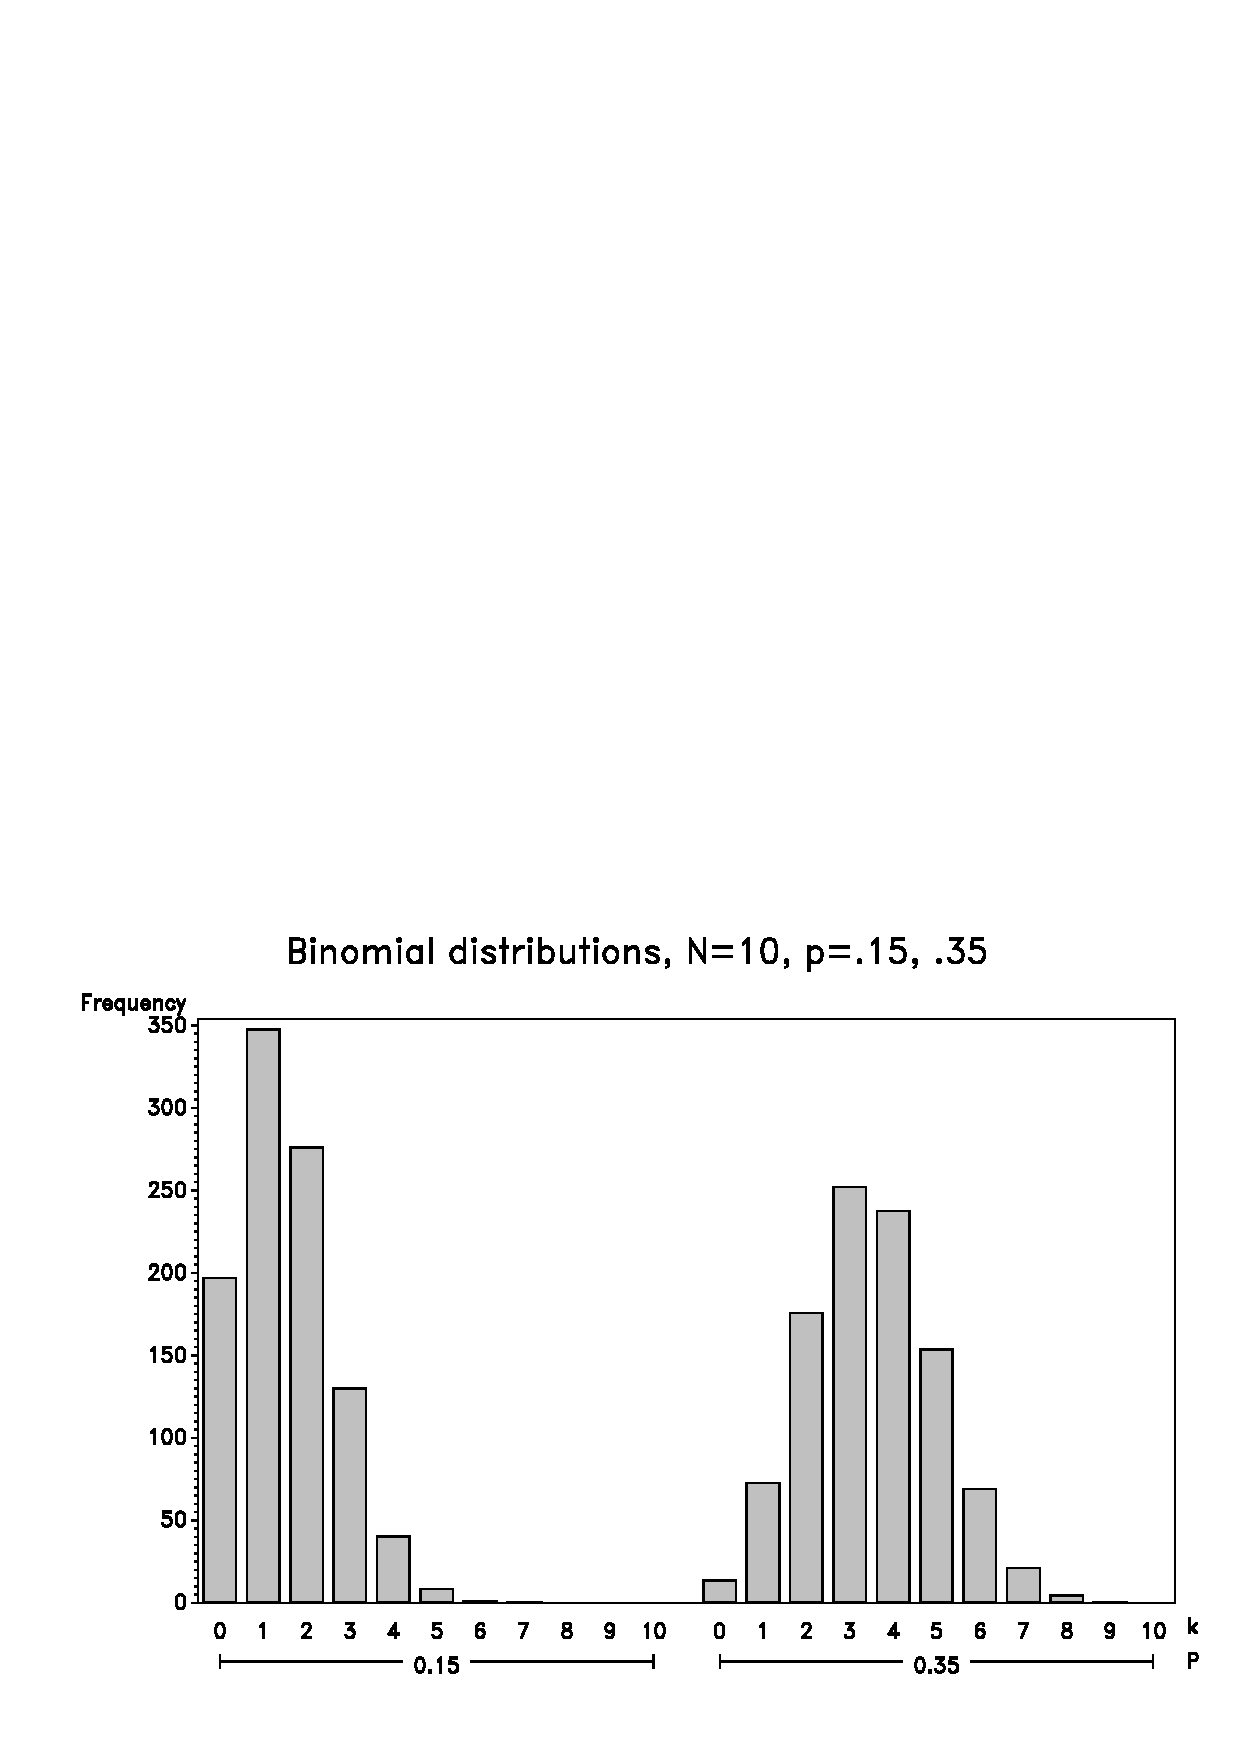
\includegraphics[scale=.75]{binomial}\graphicsfile{ch2/fig/binomial.eps}{}
  \caption{Binomial distributions for $n=10$ trials}%
  \label{fig:binomial}
\end{figure}
Alternatively, one may prefer to plot such distributions as frequency
polygons or as needle graphs, using \PROC{GPLOT}.
For example, \figref{fig:binomial2} shows frequency polygons for
the binomial distributions $\Bin(10,p)$ with $p = 0.15 (0.20) 0.75$,
obtained by running the \texttt{binomial} \Dstp\ with
\begin{listing}
%let p=.15 to .75 by .20;
\end{listing}
The \PROC{GPLOT} step (excluding statements for symbols, axes, and the
legend) is just
\begin{listing}
proc gplot data=binomial;
   plot freq * k = p / frame vminor=1 hminor=0 ... ;
\end{listing}

%% one figure
\begin{figure}[htb]
%  \SASfig{binomial2.eps}{scale=.75}{binomial2}{Binomial distributions for $n=10$ trials, as frequency polygons}
  \centering
  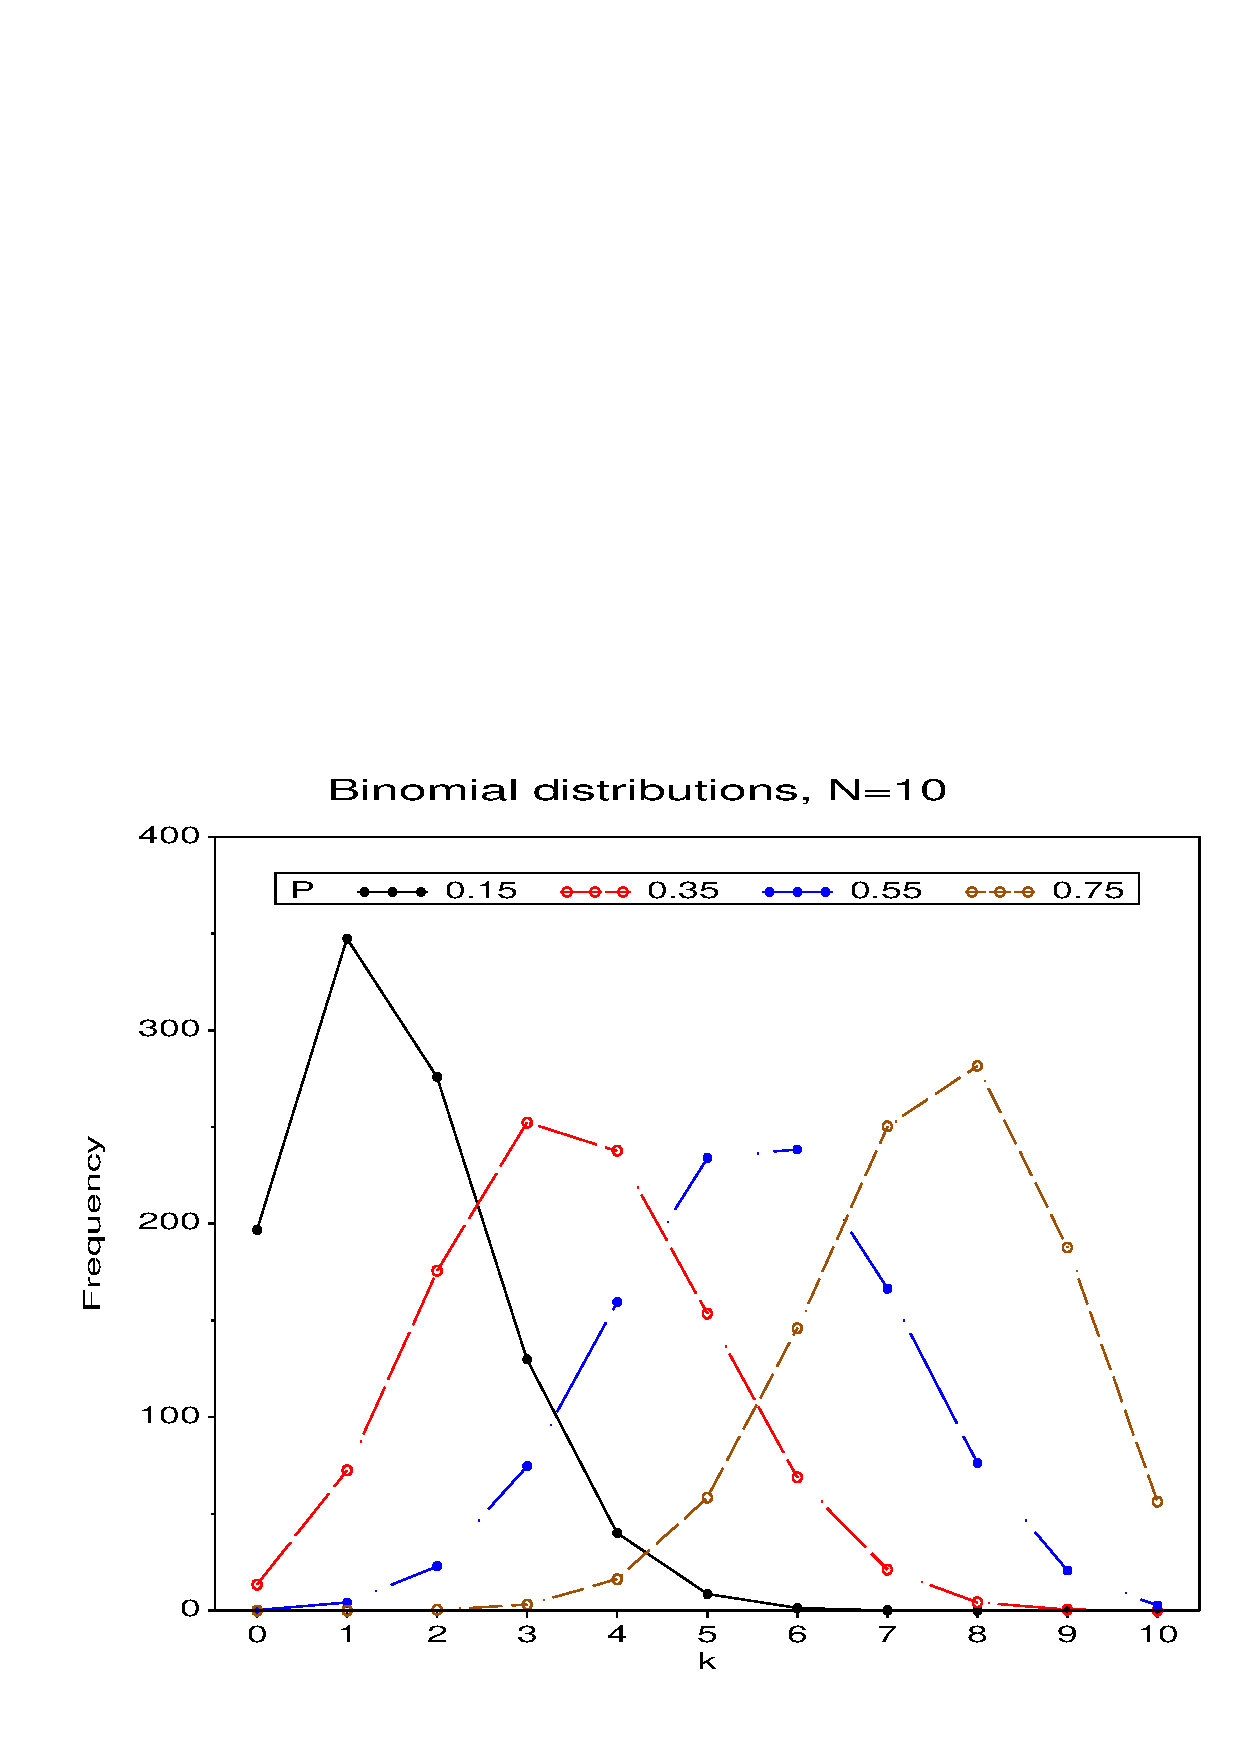
\includegraphics[scale=.75]{binomial2}\graphicsfile{ch2/fig/binomial2.eps}{}
  \caption{Binomial distributions for $n=10$ trials, as frequency polygons}%
  \label{fig:binomial2}
\end{figure}
\ix{binomial distribution!visualization|)}
\ix{binomial distribution|)}

\subsection{The Poisson distribution}
\ix{Poisson distribution|(}

The Poisson distribution gives the probability of an event occurring
$k = 0, 1, 2, \dots$ times over a large number of ``trials'',
when the probability, $p$, that the event occurs on any one
trial is very small and constant;
hence, the Poisson distribution is usually applied to the study of
rare events such as highway accidents at a particular location,
deaths from horse kicks, or defects in a well-controlled manufacturing
process.

For the \IX{Poisson distribution}, the probability function
is
\begin{equation}\label{eq:poisf}
\textrm{Pois}(\lambda):\Pr \{ X = k \} \equiv p (k)=
  \frac{ e^{ - \lambda } \:  \lambda^k } { k ! }
  \quad\quad k = 0, 1, \dots
\end{equation}
where the parameter, $\lambda$ turns out to be the mean of the
distribution.
The first three (central) moments of the Poisson distribution are
in fact all equal to $\lambda$:
\begin{eqnarray*}
\textrm{Mean}[X] & = & \lambda \\
\textrm{Var}[X] &  = & \lambda \\
\textrm{Skew}[X] & = & \lambda 
\end{eqnarray*}
%% Mathematica gives Skew = 1 / \sqrt(\lambda) ???

So, the mean and variance of the Poisson distribution are always
the same, which is sometimes used to identify a distribution
as Poisson.  For the binomial distribution, the mean ($Np$) is always
greater than the variance ($Npq$); for other distributions
(negative binomial and geometric) the mean is less than the
variance.

The maximum likelihood estimator of the parameter \(\lambda\)
in \eqref{eq:poisf} is just
the mean of the distribution,
\begin{equation*}
  \hat{\lambda}= \bar{x} = \frac{\sum_k k \,  n_k}{\sum_k  n_k}
  \period
\end{equation*}
Hence, the expected frequencies can be estimated by substituting the
sample mean into \eqref{eq:poisf}.
Moreover, Poisson variables have a nice reproductive property:
 if $X_1, X_2, \dots X_m$ are independent Poisson
variables with the same parameter $\lambda$, then their
sum, $\sum X_i$ is a Poisson variate with parameter $m \lambda$;
if the Poisson parameters differ, the sum is still Poisson with
parameter $\sum \lambda_i$.

\begin{Example}[soccer]{UK Soccer scores}
\tabref{tab:soccer1}  gives the distributions of goals scored by
the 20 teams in the  1995/96 season of the
 Premier League of the UK Football Association
as presented by
\citet{Lee:97}.%
\footnote{\citet[p. 16]{Lee:97} apparently has the home and away labels reversed in
his table.
The row and column labels in \tabref{tab:soccer1} give means of 1.48
for home teams and 1.06 for away teams.  The raw data were verified
from that listed at \url{http://users.aol.com/mabstabs/soccer.html}}
Over a season
each team plays each other team exactly once, so there are a total of
$20 \times 19 = 380$ games.
Because there may be an advantage for the home team,
the goals scored have been classified as ``home team'' goals
and ``away team'' goals in the table.
\input{ch2/tab/soccer1}

If we assume that in any small interval of time there is a small, constant
probability that the home team or the away team may score a goal,
the distributions of the goals scored by home teams
(the row totals in \tabref{tab:soccer1})
may be modeled as Pois($\lambda_H$) and the distribution of
the goals scored by away teams (the column totals)
may be modeled as Pois($\lambda_A$).

If the number of goals scored by the home and away teams are independent%
\footnote{This question
is examined visually in \chref{ch:mosaic} (\exref{ex:soccer2})
and \chref{ch:corresp} (\exref{ex:soccer3}), where we find that the answer
is ``basically, yes''.},
we would expect that the total number of goals scored in any
game would be distributed as Pois($\lambda_H + \lambda_A$).
These totals are shown in \tabref{tab:soccer2}.
As preliminary check of the distributions for the home and away goals,
we can determine if the means and variances are reasonably close
to each other.
If so, then the total goals variable should also have a mean and variance
equal to the sum of those statistics for the home and away goals.
\input{ch2/tab/soccer2}

The statements below read the data from \tabref{tab:soccer1}, calculate
the \texttt{TOTAL} goals, and find the distribution of \texttt{TOTAL} goals
shown in \tabref{tab:soccer2}.  The \PROC{MEANS} step produces the
mean and variance of each variable, shown in \outref{out:soccer1.2}.
\input{ch2/sas/soccer1}

\begin{Output}[htb]
\caption{UK Soccer data, assessing Poissonness}\label{out:soccer1.2}
\small
\verbatiminput{ch2/out/soccer1.2}
\end{Output}
The means are all approximately equal to the corresponding variances.
More to the point, the variance of the \texttt{TOTAL} score
is approximately equal to the sum of the individual variances.
Note also there does appear to be an advantage for the home team,
of nearly half a goal.
\end{Example}


\subsubsection{Calculation and visualization}
\ix{Poisson distribution!visualization|(}
Poisson probabilities may be calculated using the \FUNC{poisson},
which is called as \texttt{poisson(lambda, m)} for a distribution
with mean \texttt{lambda}.
This also returns cumulative probabilities,
$ \sum_{k=0}^{k=m} p ( k )$,
which must be differenced to calculate the probability of exactly
$m$ events.  The \FUNC{pdf}, called as \texttt{pdf('poisson', m, lambda)}
calculates these densities directly.
Random data from a poisson distribution may be obtained using the
\CALL{ranpoi}.

The \Dstp\ below illustrates the use of the \FUNC{pdf} to calculate
poisson frequencies for the distributions with means ($\lambda$) 2 and 5,
for $k = 0, 1, \dots , 12$.

%% input: /Users/friendly/sasuser/catdata/poisson1.sas
%% last modified: 07-Jul-99 13:37
\begin{listing}
%let N=12;
%let lambda = 2, 5;
title "Poisson distributions, lambda=&lambda, k=0..&N";
data poisson;
   reps = 1000;
   drop reps;
   N=&N;
   do lambda=&lambda;
      do k=0 to N;
         prob = pdf('poisson', k, lambda);
         freq = reps * prob;
         output;
         end;
      end;
   label freq='Frequency'
        lambda='Lambda'
        k = 'k';
\end{listing}

\begin{figure}[htb]
  \centering
  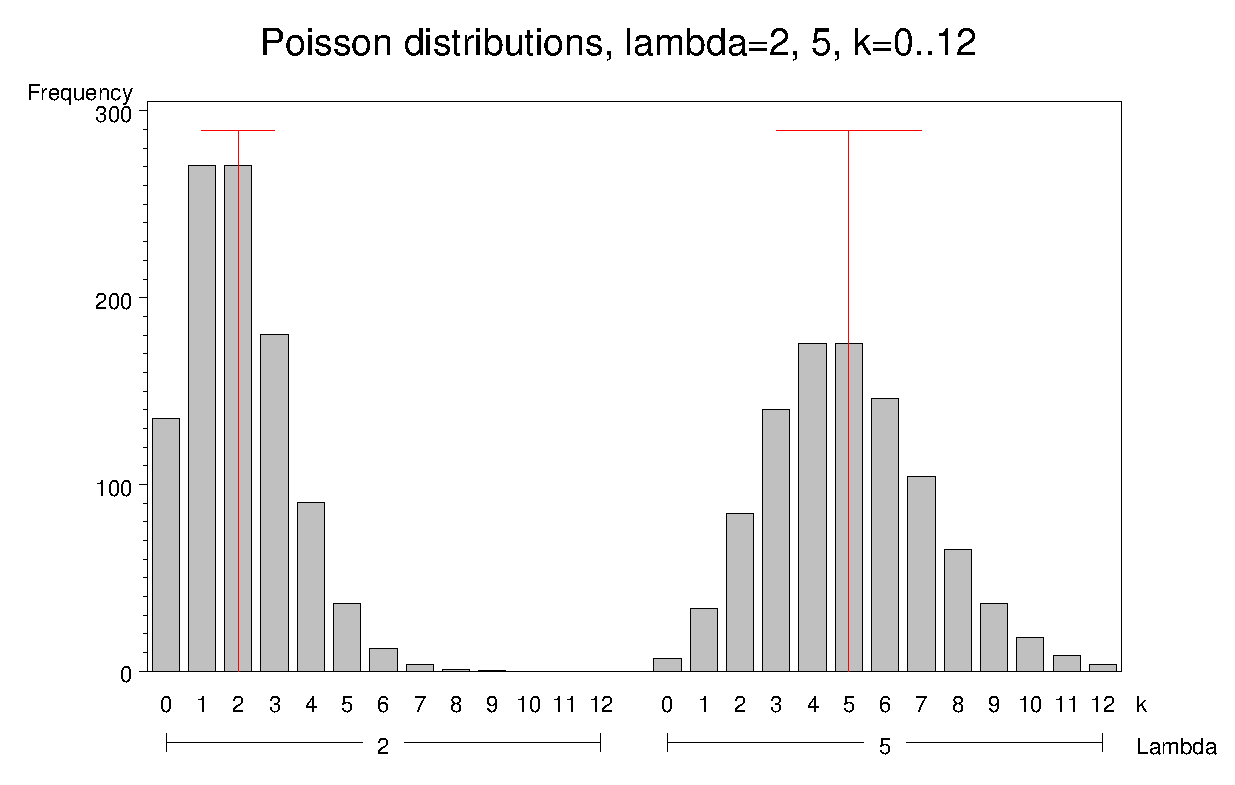
\includegraphics[scale=.75]{poisson1}\graphicsfile{ch2/fig/poisson1.eps}{}
  \caption[Poisson distributions with $\lambda =$ 2, 5.]{Poisson distributions with $\lambda =$ 2 and 5.  The vertical line shows the mean
  of each distribution; the horizontal lines show the standard deviation.}%
  \label{fig:poisson1}
\end{figure}

These distributions are shown in \figref{fig:poisson1},
plotted using \PROC{GCHART} as shown earlier for the binomial
distribution.
\ix{Poisson distribution!visualization|)}
\ix{Poisson distribution|)}

\subsection{The negative binomial distribution}
\ix{negative binomial distribution|(}

The negative binomial distribution is a type of waiting-time distribution.
One form of
the negative binomial distribution
(also called the Pascal distribution) arises when a series of Bernoulli
trials is observed with constant probability $p$ of some event,
and we ask how many trials it takes to observe
$n$ events.
The probability function with parameters $n$ (an integer, $0 < n < \infty$) and $p \, (0 < p < 1)$
gives the probability that $k$ non-events (failures) are observed before
the $n$-th event (success), and
can be written
\begin{equation}\label{eq:negbinf}
\NBin(n,p):   \Pr \{ X = k \} \equiv p(k)  =
  {n+k-1 \choose k} p^n (1-p)^k
  \quad\quad k = 0, 1, \dots , \infty
\end{equation}

The moments of the negative binomial distribution are:
\begin{eqnarray*}
\textrm{Mean}[X] &=&nq / p \\
\textrm{Var}[X] &=&nq / p^2 \\
\textrm{Skew}[X] &=&\frac{2-p}{\sqrt{nq}}
\comma
\end{eqnarray*}
where $q=1-p$.

A more general form of the negative binomial distribution
allows $n$ to take non-integer values and to be an unknown
parameter.
In this case, the combinatorial coefficient,
${n+k-1 \choose k}$ in \eqref{eq:negbinf} is calculated using
the gamma function, $\Gamma(\bullet)$,
a generalization of the factorial for non-integer values,
defined so that $\Gamma(x+1) = x!$ when $x$ is an integer.
Then the probability function \eqref{eq:negbinf} becomes
\begin{equation}\label{eq:negbinf2}
  \Pr \{ X = k \} \equiv p(k)  =
  \frac{\Gamma(n+k)}{\Gamma(n) \Gamma(k+1)}
   p^n (1-p)^k
  \quad\quad k = 0, 1, \dots , \infty
  \period
\end{equation}

In this form, the negative binomial distribution is frequently used
as an alternative to the Poisson distribution when the assumptions
of the Poisson (constant probability and independence) are not
satisfied, or when the variance of the distribution is greater
than the mean (termed \glossterm{overdispersion}).
\citet{GreenwoodYule:20}
developed the negative binomial distribution as a model for
accident proneness or susceptibility of individuals to
repeated attacks of disease.
They assumed that for any individual the number of accidents
or disease occurrences has a Poisson distribution with parameter
$\lambda_i$.
If individuals vary in proneness, so that the $\lambda_i$ have
a gamma distribution, the resulting distribution is the
negative binomial.

When both $n$ and $p$ are treated as unknown parameters,
maximum likelihood estimators are available, but involve
complex non-linear equations.
The simpler method of moments estimators
are
\begin{eqnarray*}
  \hat{p} & = & \bar{x} / s^2 \\
  \hat{n} & = & \bar{x}^2 / ( s^2 - \bar{x} )
  \comma
\end{eqnarray*}
where $\bar{x}$ and $s^2$ are the sample mean and variance of the observed
distribution.
Note that if $s^2 < \bar{x}$, the estimate of $n$ will be negative
and that of $p$ will be greater than 1, so the negative binomial
distribution should be considered inappropriate.

\subsubsection{Calculation and visualization}
The SAS \FUNC{probnegb} calculates negative binomial cumulative probabilities for
integer values of the number of successes parameter, $n$.
To calculate probabilities for individual values of $k$, it is necessary
to compute the difference between successive values $k-1$ and $k$,
as with the binomial and Poisson distribution functions,
or use the \FUNC{pdf}, called as \texttt{pdf('negbinomial', k, p, n)}.
For non-integer values of $n$ it is necessary to calculate the probabilities
directly using \eqref{eq:negbinf2}.
Random values from a negative binomial distribution may be obtained by
calculating the probabilities, $p(k), k=0, 1, \dots$ and
using these with the \FUNC{rantbl}.

\figref{fig:probnegb} shows negative binomial distributions for the number of
trials to observe  $n=2$ or $n=4$ successes with $p = .2, .3, .4$, and
with values of $k$ from 0 to 20.
The vertical line in each panel marks the location of the mean; the horizontal
line shows the range of one standard deviation about the mean.

%% one figure
\begin{figure}[htb]
% \SASfig{probnegb.eps}{scale=.8}{probnegb}{Negative binomial distributions for the number of trials to observe  {\protect{$n=2$ or $n=4$} successes}}
  \centering
  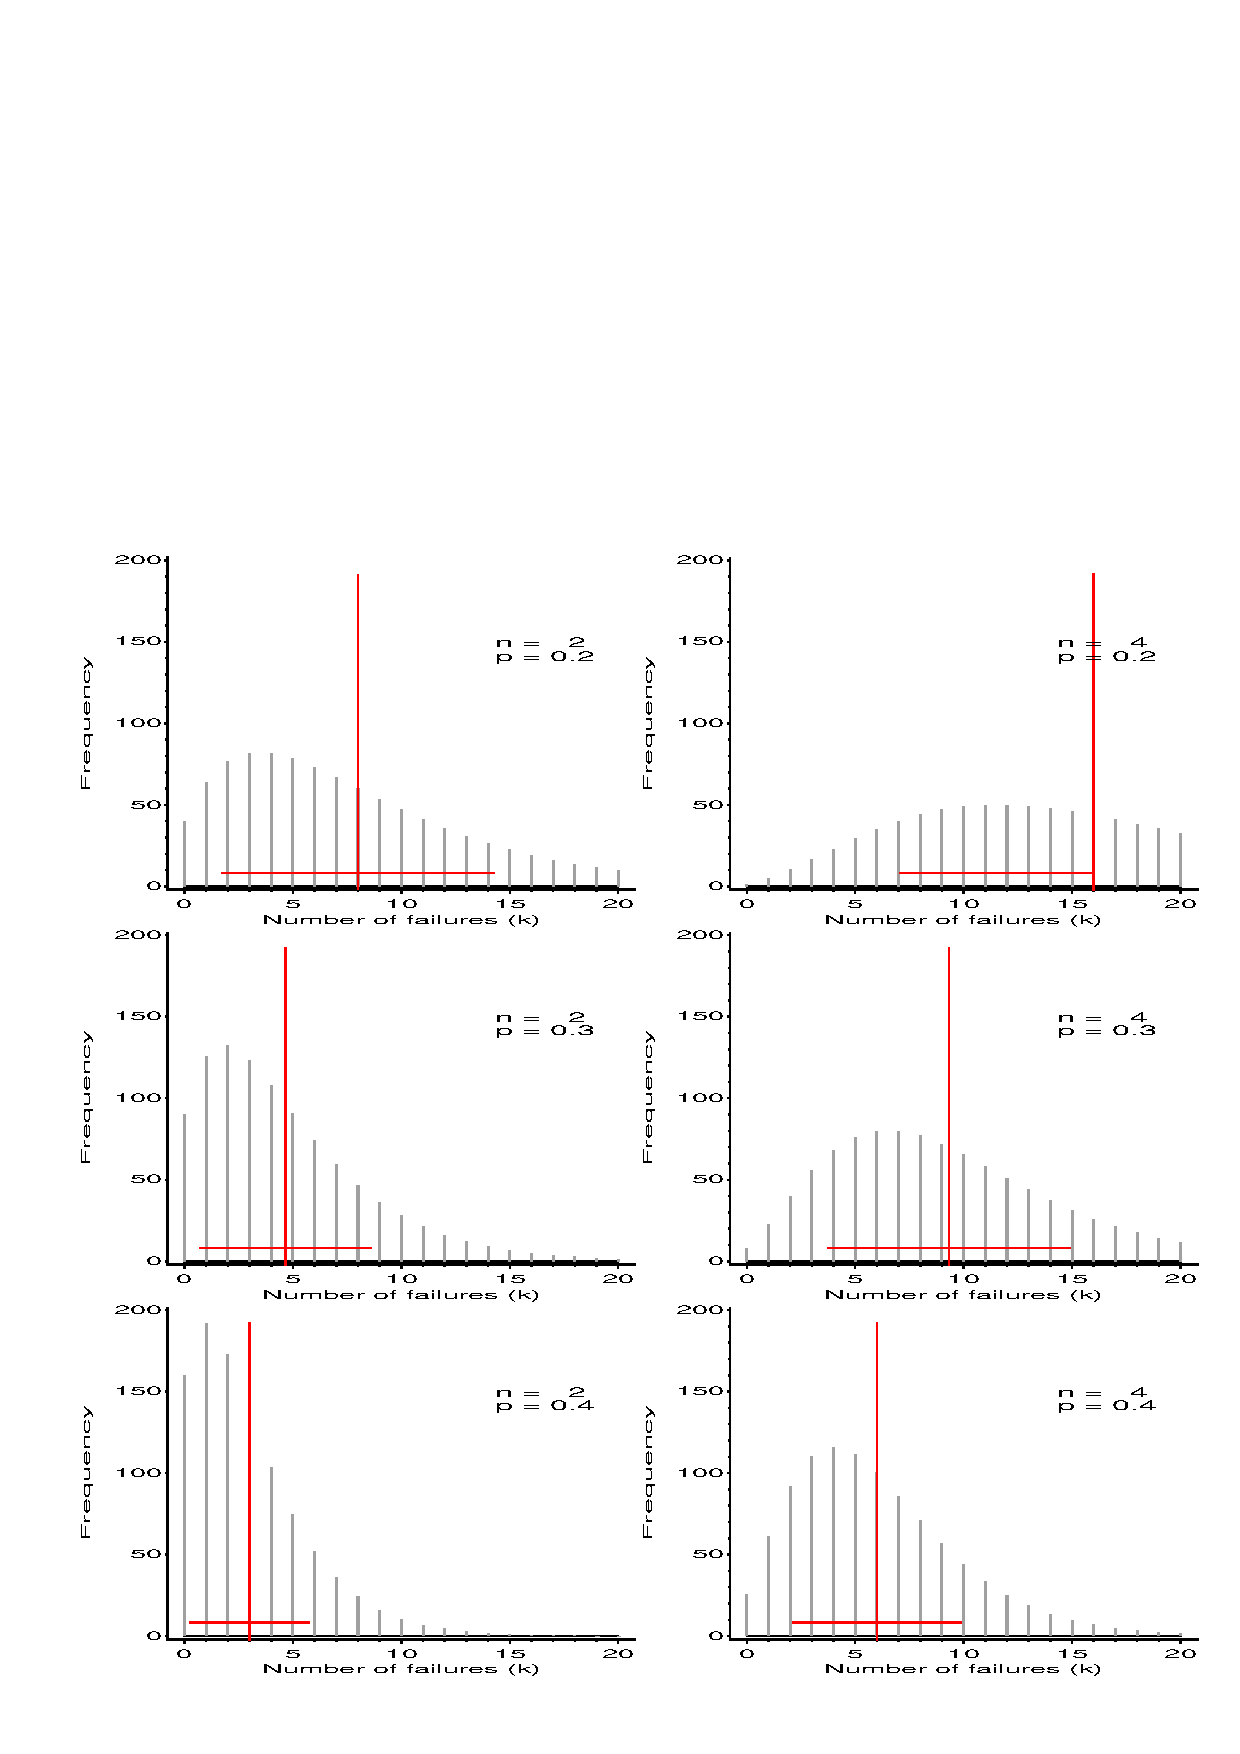
\includegraphics[scale=.8]{probnegb}\graphicsfile{ch2/fig/probnegb.eps}{}
  \caption{Negative binomial distributions for
        the number of trials to observe {\protect{$n=2$ or $n=4$} successes}}%
  \label{fig:probnegb}
\end{figure}
\ix{negative binomial distribution|)}

\subsection{The geometric distribution}
\ix{geometric distribution|(}
The special case of the negative binomial distribution when $n=1$
is a geometric distribution.
We observe a series of independent trials and count the number
of non-events (failures) preceding the first successful event.
The probability that there will be  $k$ failures before the first
success
is given by
\begin{equation}\label{eq:geomf}
\textrm{Geom}(p):   \Pr \{ X = k \} \equiv p ( k )  =
   p (1-p)^k
  \quad\quad k = 0, 1, \dots
  \period
\end{equation}
For this distribution,
\begin{eqnarray*}
\textrm{Mean}[X] & = & 1 / p\\
\textrm{Var}[X] &  = & (1-p) / p^2 \\
\textrm{Skew}[X] & = & (2-p) / \sqrt{1-p}
\end{eqnarray*}
\ix{geometric distribution|)}

\subsection{The logarithmic series distribution}
\ix{logarithmic series distribution|(}
The logarithmic series distribution is a long-tailed distribution
introduced by
\citet{Fisher-etal:43}
in connection with data on the abundance of individuals
classified by species of the type shown for the distribution of butterfly
species
in \tabref{tab:butterfly}.

The probability distribution function with parameter $\theta$ is given by
\begin{equation}\label{eq:logseriesf}
\textrm{LogSer}(\theta): \Pr \{ X = k \} \equiv p ( k )  =
\frac{\theta ^k}{-(k\log (1-\theta ))} =
\alpha \theta^k / k
\quad\quad k = 1, 2, \dots, \infty
\comma
\end{equation}
where $\alpha = -1 / \log(1 - \theta)$
and $0 < \theta <1$.
Fisher derived the logarithmic series distribution by assuming that
for a given species the number of individuals trapped has a Poisson
distribution with parameter $\lambda = \gamma t$, where
$\gamma$ is a parameter of the species (susceptibility to entrapment)
and $t$ is a parameter of the trap.
If different species vary so that the parameter $\gamma$ has a gamma
distribution, then the number of representatives of each species trapped
will have a negative binomial distribution.
However, the observed distribution is necessarily truncated on the left,
because one cannot observe the number of species never caught (where $k=0$).
The logarithmic series distribution thus arises as a limiting form of the
zero-truncated negative binomial.

From \eqref{eq:logseriesf}
\begin{equation*}
\frac{p(k+1)}{p(k)} = \frac{k \theta}{k+1} < 1
\comma
\end{equation*}
for all $k$, since $\theta < 1$.  Hence, the maximum probability occurs at $k=1$
and $p(k)$ decreases steadily as $k$ increases.

The mean and variance of the distribution are
\begin{eqnarray}
\textrm{Mean}[X] & = & \alpha \theta / (1-\theta ) \equiv \mu \label{eq:logsermean}\\
\textrm{Var}[X] & = &  \alpha \theta (1-\alpha\theta) / (1-\theta )^2
= \mu ( \frac{1}{1-\theta} - \mu )
\nonumber
\end{eqnarray}

In fitting this distribution to data, the method of moments and maximum likelihood
both involve equating the sample mean to the population mean in \eqref{eq:logsermean},
a nonlinear equation which must be solved numerically for $\theta$.
When $\bar{x} < 25$, an approximation given by
\citet{Birch:63},
\begin{equation*}%\label{eq:thetabirch}
\hat\theta  \approx
1 - \frac{1}{1 + [ ( \frac{5}{3} - \frac{1}{16}\log \bar{x}) (\bar{x}-1) + 2 ] \log \bar{x} }
\period
\end{equation*}

Another useful unbiased approximation is based on the proportion of observations
at $k=1$,
\begin{equation*}
\hat\theta  \approx 1- \frac{n_1 / N}{\bar{x}}
\period
\end{equation*}
\ix{logarithmic series distribution|)}

\subsection{Power series family}\label{sec:pwrseries}
\ix{power series distributions|(}

I mentioned earlier that the Poisson distribution was unique among all discrete (one parameter) distributions, in that it is the only one whose mean and variance are equal
\citep{Kosambi:49}.
The relation between mean and variance of discrete distributions also provides
the basis for integrating them into a general family.
All of the discrete distributions described in this section are in fact
special cases of a family of discrete distributions
called the power series distributions by
\citet{Noack:50}
and defined by
\begin{equation*}
p(k) = a(k) \theta^k / f(\theta)
\quad\quad k=0, 1, \dots \comma
\end{equation*}
with parameter $\theta > 0$,
where $a(k)$ is a coefficient function depending only on $k$
and $f ( \theta) = \sum_k a(k) \theta^k$ is called the series
function.  The definitions of these functions are shown in
\tabref{tab:pwrseries}.
\begin{table}[!tb] \centering%
\caption{The Power Series family of discrete distributions\label{tab:pwrseries}}%
\small
\begin{tabular}{lllll}\hline
Discrete & Probability  & Series  & Series  & Series \\ 
Distributiion & function, $p(k)$ & parameter, $\theta$ &
function, $f(\theta )$ & coefficient, $a(k)$ \\ \hline
%
Poisson & $e^{-\lambda }\lambda ^k/k!$ & $\theta = \lambda$ & $e^\theta $ & $1/k!$ \\[1ex] 
Binomial & $\binom nkp^k(1-p)^{n-k}$ & $\theta = p / (1-p) $ & $(1+\theta )^n$ & $\binom nk$ \\[1ex] 
Negative binomial & $\binom{n+k-1}kp^n(1-p)^k$ &  $\theta = (1-p) $ & $(1-\theta )^{-k}$ & $%
\binom{n+k-1}k$ \\[1ex] 
Geometric & $p(1-p)^k$ &  $\theta = (1-p)$ & $(1-\theta )^{-k}$ & $1$ \\[1ex]
Logarithmic series & $\theta ^k/[-k\log (1-\theta )]$ &  $\theta = \theta$ & $-\log (1-\theta )$
& $1/k$ \\[1ex] \hline
\end{tabular}
%TCIMACRO{\TeXButton{E}{\end{table}}}
%BeginExpansion
\end{table}%
%EndExpansion



These relations among the discrete distribution provide the basis for
graphical techniques for diagnosing the form of discrete data described
later in this chapter (\secref{sec:discrete-other}).
\ix{power series distributions|)}

\section{Fitting discrete distributions}\label{sec:discrete-fit}

Often interest is focused on how closely such data follow a
particular distribution, such as the Poisson, binomial, or geometric
distribution.  Usually this is examined with a classical (Pearson)
goodness-of-fit chi-square test,
\glosstex{chi-square test}

\begin{equation}\label{eq:chi2}
  \chi^2 = \sum_{k=1}^K \:
  \frac{{ ( n_k - N \hat{p}_k ) }^2}
  { N \hat{p}_k }  \sim \chi^2_{( K-s-1 )}
  \comma
\end{equation}
where there are $K$ frequency classes, 
$s$ parameters have been estimated from the data and
\(\hat{p}_k\) is the estimated probability of each basic count,
under the null hypothesis that the data follows the chosen distribution.
An alternative test statistic is the likelihood-ratio $G^2$
statistic,
\begin{equation}\label{eq:g2}
 G^2 = \sum_{k=1}^K \: n_k \log ( n_k / N \hat{p}_k )
 \comma
\end{equation}
when the $\hat{p}_k$ are estimated by maximum likelihood,
which also has an asymptotic $\chi^2_{(K - s - 1)}$ distribution.
``Asymptotic'' means that these are large sample tests.
A common rule of thumb is that all expected frequencies
should exceed one and that fewer than 20\% should be less than 5.

For the horse kick data, the mean is 122/200 = .610, and calculation
of Poisson probabilities (\texttt{PHAT}), expected frequencies, and
contributions to \(\chi^2\) \eqref{eq:chi2} are shown below.
\ixd{deaths by horsekick}

\begin{center}
\begin{alltt}
 k     nk      p        phat         exp     chisq

 0    109    0.545    0.54335    108.670    0.00100
 1     65    0.325    0.33144     66.289    0.02506
 2     22    0.110    0.10109     20.218    0.15705
 3      3    0.015    0.02056      4.111    0.30025
 4      1    0.005    0.00313      0.627    0.22201
      ===                        =======    =======
      200                        199.915    0.70537 \(\sim \chi\sp2 (3)\)
\end{alltt}
\end{center}

In this case the \(\chi^2\) shows an exceptionally good (perhaps unreasonably
good?) fit.  In the word frequency example
(\exref{ex:madison1}), the fit of the Poisson
turns out not to be close at all.  However, even a close fit may show
something interesting, if we know how to look; conversely, it is
useful to know why or where the data differ from a chosen model.

\subsection{The \macro{GOODFIT}}
The \macro{GOODFIT} (see \macref{mac:goodfit}) carries out Pearson \chisq{} and \LR{} goodness-of fit tests
for the uniform, binomial, Poisson, negative binomial,
 logarithmic series, and geometric distributions,
as well as any discrete (multinomial) distribution whose probabilities you can specify.
The data may consist either of individual observations on a single
variable, or a grouped frequency distribution in the form
shown in \tabref{tab:horskick}.
The parameter(s) of the distribution may be specified as constants
or may be estimated from the data.

\begin{comment}  %%% begin stuff deleted
The macro is used as follows%
\footnote{In subsequent descriptions of macros in the text
we simply give references to the documentation provided in Appendix \ref{ch:macros} and provide examples of usage.}%
:
\aunote{Should we take this out?}
\begin{listing}
\%goodfit(data=\emph{SASdatasetname},
   var=\emph{variablename},
   freq=\emph{variablename},
   dist=\emph{distribution},
   parm=\emph{parameters},
   sumat=\emph{value},
   format=\emph{SASformat},
   out=\emph{outputdatasetname},
   outstat=\emph{statisticsdatasetname});
\end{listing}
\end{comment}  
The macro parameters are described in \macref{mac:goodfit}.
We illustrate its use in \exref{ex:weldon} and \exref{ex:federalist} below.

\begin{Example}[weldon]{Weldon's dice}
The data from \tabref{tab:dice}
can be fit to a binomial distribution as shown below.
Note that, because the frequencies have been lumped for 10--12
successes, it is necessary to
\begin{seriate}
\item Input frequencies for all values of $k = 0, \dots, 12$,
using missing values for the frequencies beyond $k=10$;
\item specify \texttt{sumat=10} in the macro call.
\end{seriate}
\input{ch2/sas/dice}

The first call to the \macro{GOODFIT} fits the binomial distribution
with parameter $p = \frac13$, assuming the dice to be fair,
and produces the output shown in \outref{out:dice.1} and \outref{out:dice.2}.
The \chisq{} statistics indicate that the fit is poor,
and the pattern of residuals
suggests that $p > \frac13$
(the observed frequencies for larger values of $k$ are all
greater than the expected frequencies).
\begin{Output}
\caption{Fitting Binomial(12,$\frac13$) to Weldon's dice data: Observed and fitted frequencies}\label{out:dice.1}
\verbatiminput{ch2/out/dice.1}
\end{Output}
\begin{Output}
\caption{Fitting Binomial(12,$\frac13$) to Weldon's dice data: Goodness of fit tests}\label{out:dice.2}
\verbatiminput{ch2/out/dice.2}
\end{Output}

The second call to the \macro{GOODFIT} allows the
 parameter $p$ to be estimated from the data, giving $\hat{p} = .3377$,
and produces the output shown in \outref{out:dice.3} and \outref{out:dice.4}.
The fit is much better---in fact, quite satisfactory.
So, Weldon's dice differed minutely from being absolutely fair,
but with over 26,000 tosses it is easy to detect the difference.
\begin{Output}
\caption{Fitting Binomial(12,$p$) to Weldon's dice data: Observed and fitted frequencies}\label{out:dice.3}
\verbatiminput{ch2/out/dice.3}
\end{Output}
\begin{Output}
\caption{Fitting Binomial(12,$p$) to Weldon's dice data: Goodness of fit tests}\label{out:dice.4}
\verbatiminput{ch2/out/dice.4}
\end{Output}
\end{Example}

\begin{Example}[federalist]{Federalist papers}
The data on the occurrences of the word \emph{may} in Madison's
Federalist Papers (\tabref{tab:madison})
are fit to both the Poisson and Negative binomial distributions as shown below.  In each case, the parameters are estimated from the data.  The output for the Poisson distribution appears
in \outref{out:madfit.1} and \outref{out:madfit.2}.
The results for the Negative binomial distribution appear
in \outref{out:madfit.3} and \outref{out:madfit.4}.
\begin{listing}
%include catdata(madison);
%goodfit(data=madison, var=count, freq=blocks, dist=poisson);

%goodfit(data=madison, var=count, freq=blocks, dist=negbin);
\end{listing}

\begin{Output}
\caption{Fitting the Poisson($\lambda$) to the Federalist Papers data: Observed and fitted frequencies}\label{out:madfit.1}
\small
\verbatiminput{ch2/out/madfit.1}
\end{Output}
\begin{Output}
\caption{Fitting the Poisson($\lambda$) to the Federalist Papers data: Goodness of fit tests}\label{out:madfit.2}
\verbatiminput{ch2/out/madfit.2}
\end{Output}

\begin{Output}
\caption{Fitting the Negative binomial($n, p$) to the Federalist Papers data: Observed and fitted frequencies}\label{out:madfit.3}
\small
\verbatiminput{ch2/out/madfit.3}
\end{Output}
\begin{Output}
\caption{Fitting the Negative binomial($n, p$) to the Federalist Papers data: Goodness of fit tests}\label{out:madfit.4}
\small
\verbatiminput{ch2/out/madfit.4}
\end{Output}
\end{Example}

\subsection{Plots of observed and fitted frequencies}
Plots of the observed and fitted frequencies can help to show
both the shape of the theoretical distribution we have fitted and the
pattern of any deviations between our data and theory.

\figref{fig:madfit1} shows the fit of the Poisson distribution to the Federalist papers data, using one common form of plot that is sometimes
used for this purpose.
In this plot, observed frequencies are shown by bars and fitted
frequencies are shown by points, connected by a smooth (spline)
curve.%
%\footnote{Using a curve has the unfortunate }

Such a plot, however, is dominated by the largest frequencies,
making it hard to assess the deviations among the smaller frequencies.
To make the smaller frequencies more visible, \citet{Tukey:77}
suggest plotting the frequencies  on a square-root scale,
which he calls a \emph{rootogram} (see \figref{fig:madfit2}).
An additional improvement is to move the rootogram bars so their tops
are at the expected frequencies (giving a \emph{hanging rootogram}, \figref{fig:madfit3}).
This has the advantage that we can more easily judge the pattern
of departures against the horizontal reference line at 0, than
against the curve.
A final variation is to emphasize the differences between the
observed and fitted frequencies by drawing the bars to show the
gaps between the 0 line and the (observed-expected) difference
(\figref{fig:madfit4}).

These plots are produced by the \macro{ROOTGRAM} using the (default)
\texttt{OUT=FIT}
\Dset\ from the \macro{GOODFIT}:
\input{ch2/sas/madfit1}

% subfigmatrix 2 x 2
\begin{figure}[htb]
 \begin{subfigmatrix}{2}
 \subfigure[Histogram]{\label{fig:madfit1}%
  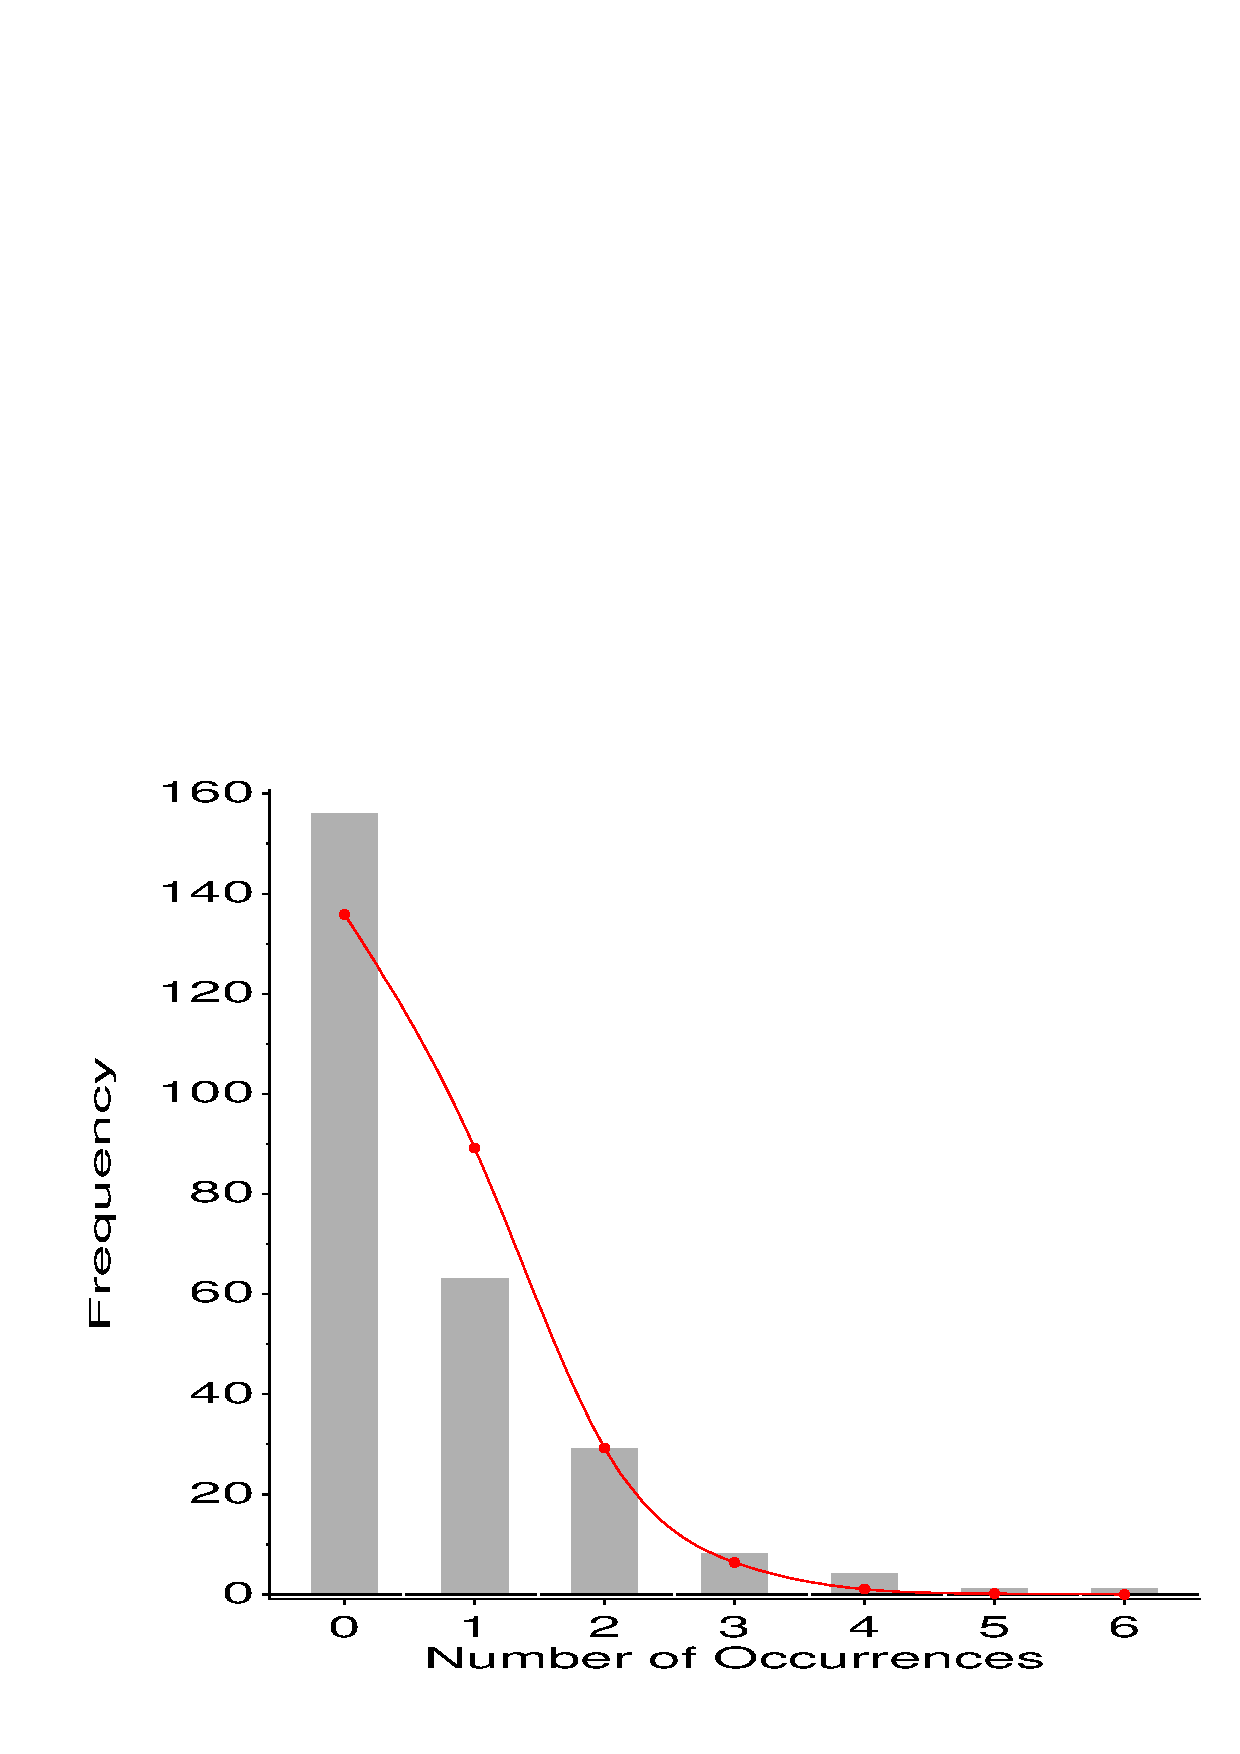
\includegraphics{madfit1}\graphicsfile{ch2/fig/madfit1.eps}{}
 }
 \subfigure[Rootogram]{\label{fig:madfit2}%
  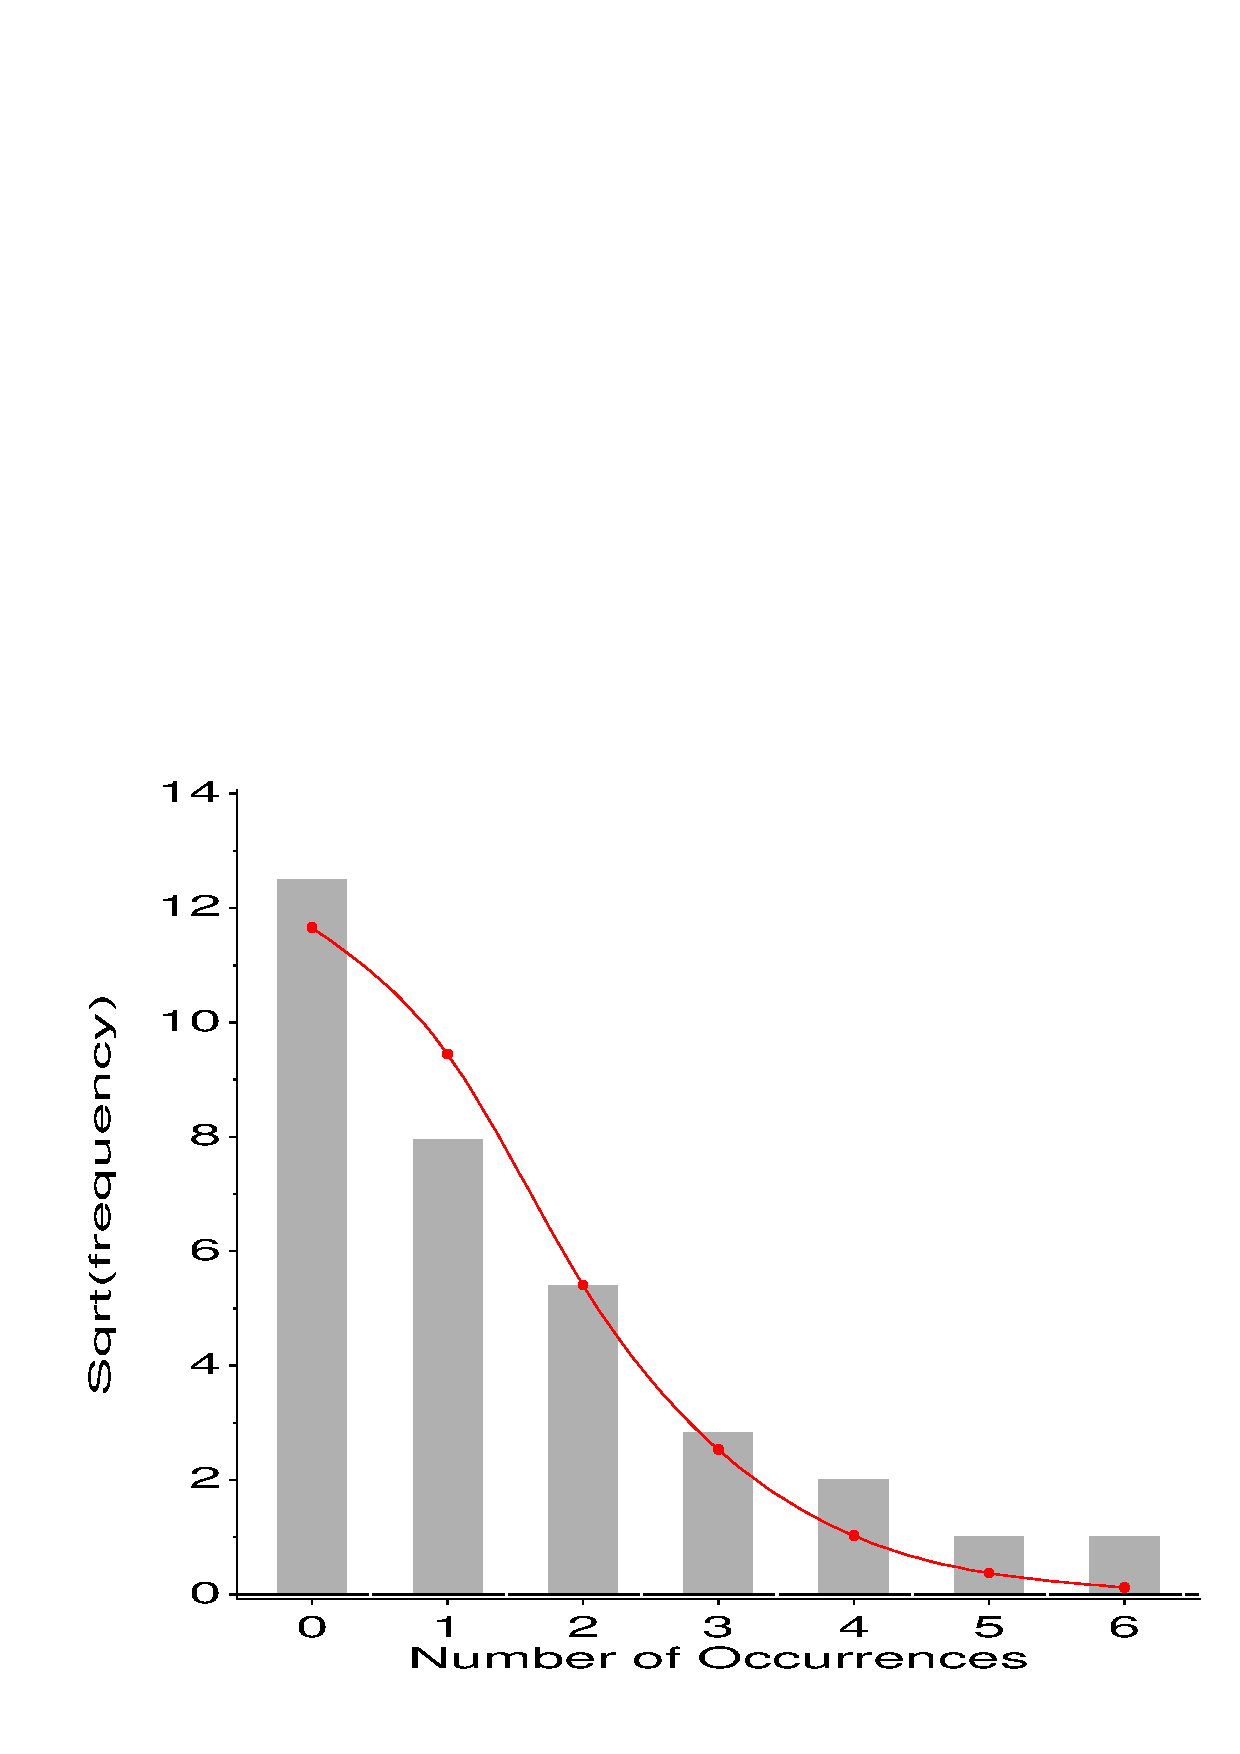
\includegraphics{madfit2}\graphicsfile{ch2/fig/madfit2.eps}{}
 }
 \subfigure[Hanging rootogram]{\label{fig:madfit3}%
  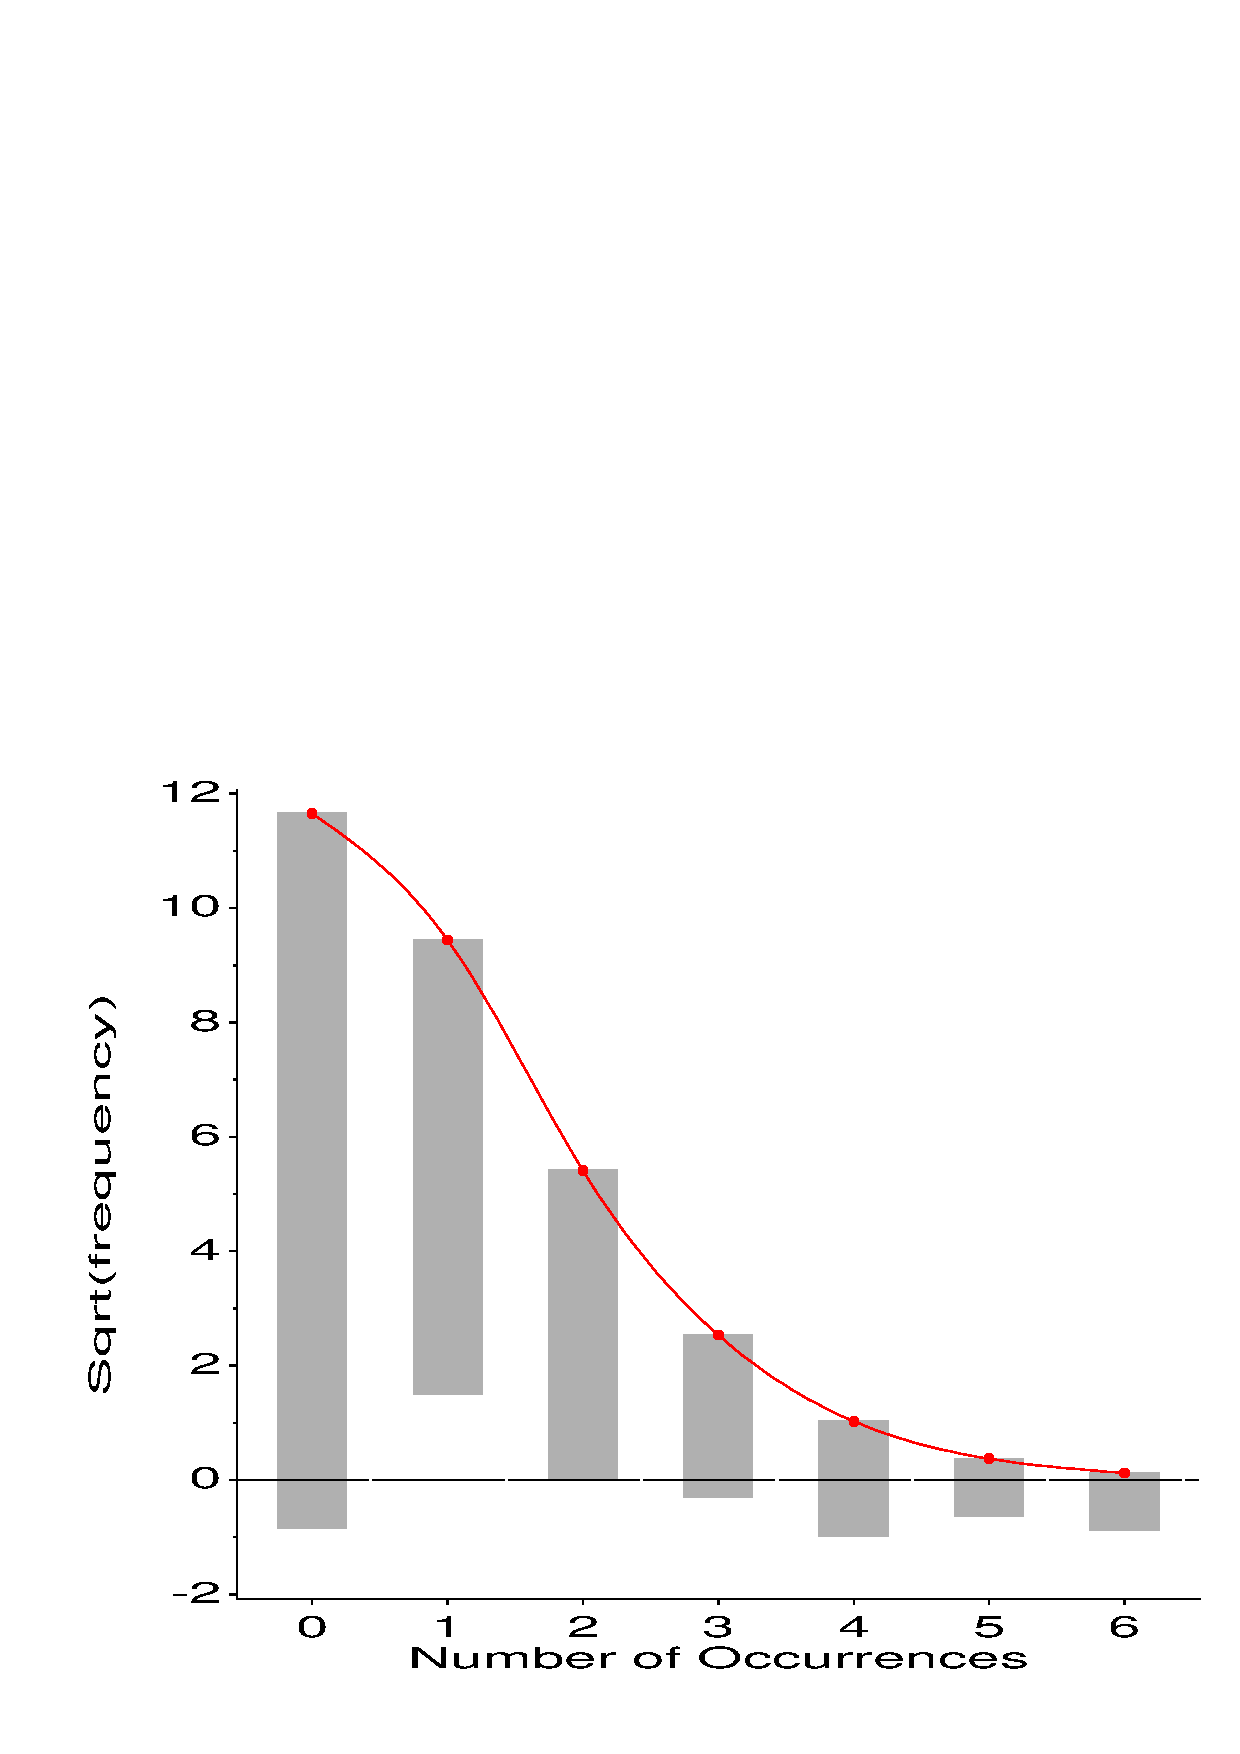
\includegraphics{madfit3}\graphicsfile{ch2/fig/madfit3.eps}{}
 }
 \subfigure[Deviation rootogram]{\label{fig:madfit4}%
  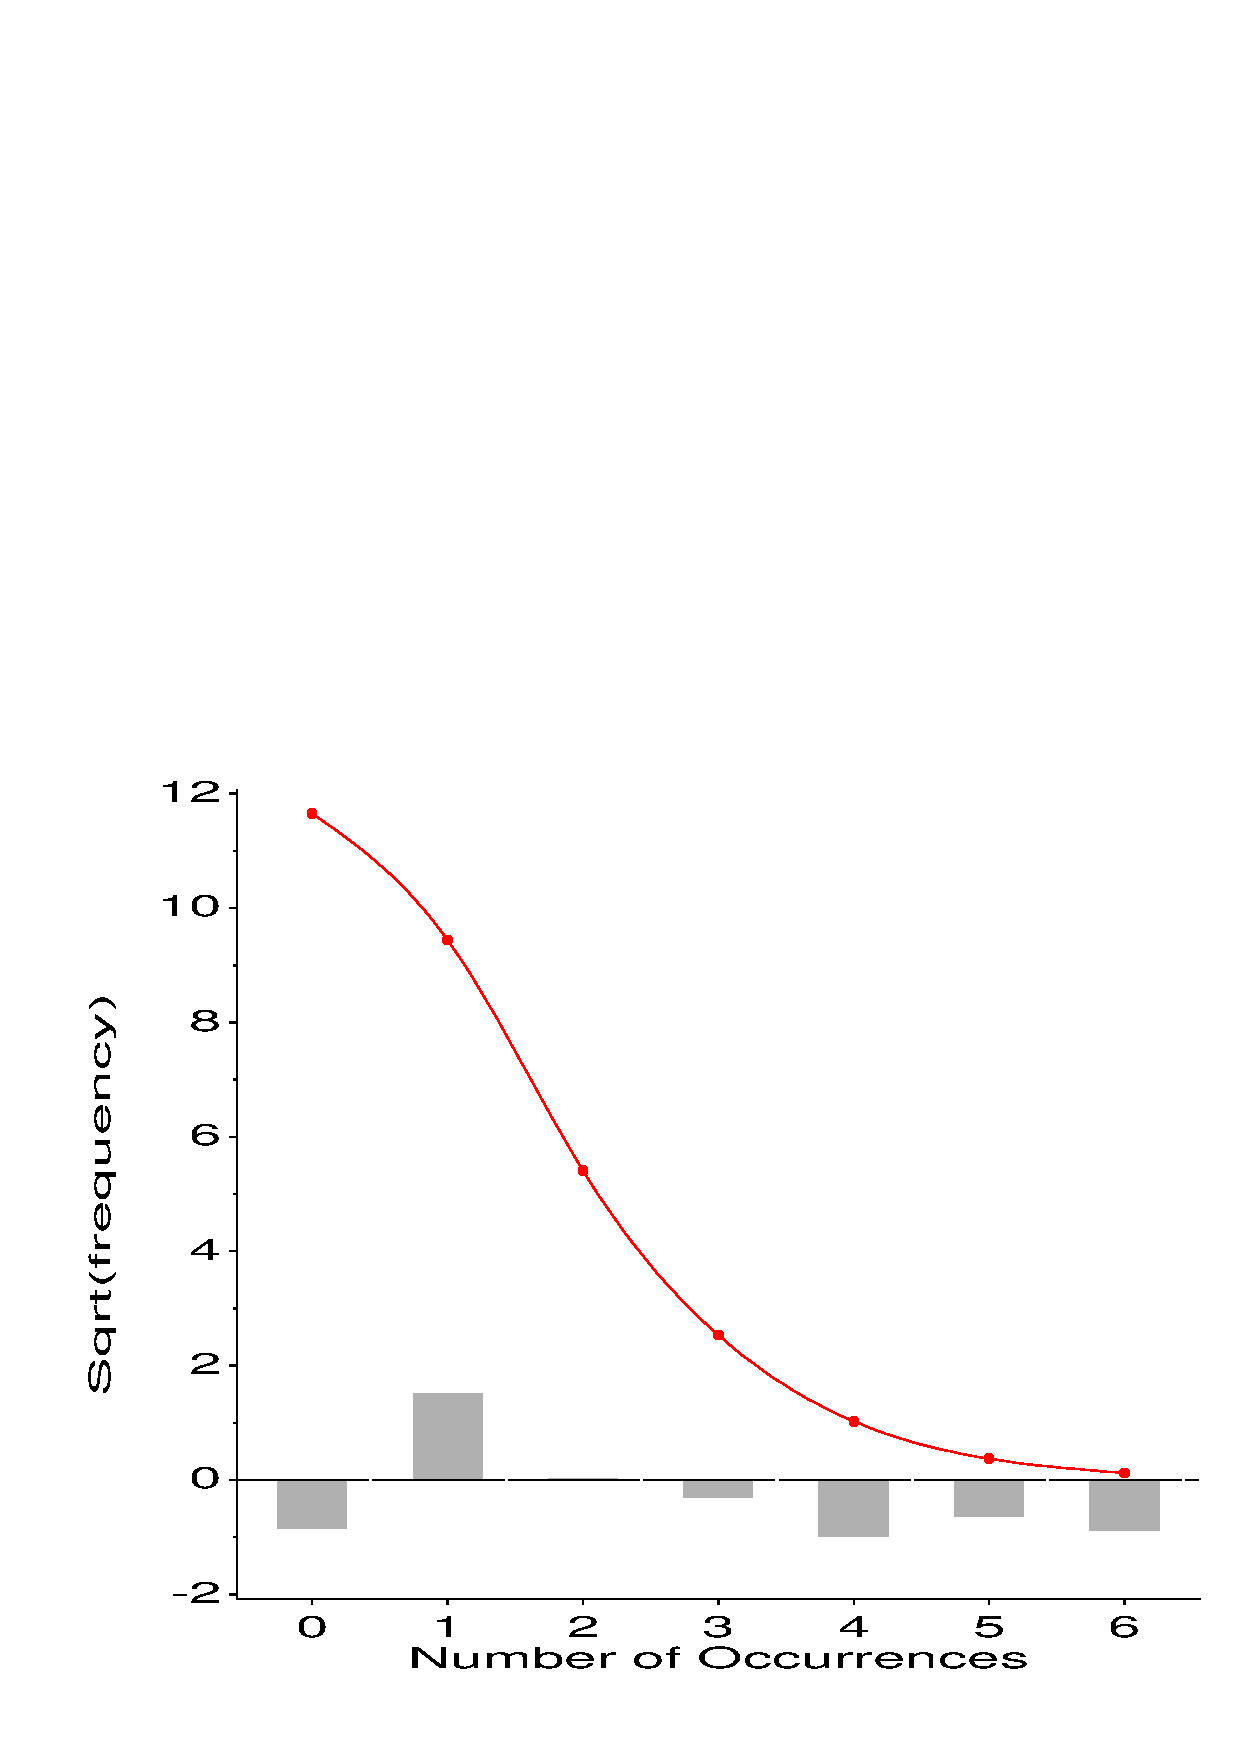
\includegraphics{madfit4}\graphicsfile{ch2/fig/madfit4.eps}{}
 }
 \end{subfigmatrix}
 \caption[Plots of observed and fitted frequencies]{Plots of observed and fitted frequencies
 for the Federalist Papers data, Poisson model.  Each panel shows the fitted frequencies as a smooth
 curve and observed frequencies as a bar.  Panel (a) raw frequencies;
 panels (b)-(d) on a square-root scale, to emphasize smaller frequencies.  Panel (c) is a hanging rootogram, where observed - fitted differences can be judged relative to the horizontal line. Panel (d) shows only the difference between the observed and fi

tted frequency.}\label{fig:madfit}
\end{figure}


\subsection{The \macro{ROOTGRAM}}\label{discrete-root}
The \macro{ROOTGRAM} (\macref{mac:rootgram}) displays observed and fitted frequencies
for a \Dset\ in any of the forms shown in \figref{fig:madfit}.
The input \Dset\ is usually of the form of the output
\texttt{OUT=} \Dset\ produced by the \macro{GOODFIT}.

\begin{Example}[federalist2]{Federalist papers}
We have seen that the negative binomial produces a better fit to the
Federalist Papers data.  The hanging rootogram (\figref{fig:madfit5}),
produced by the statements below, is characteristic of a decent fit.
\begin{listing}
%include catdata(madison);
%goodfit(data=madison, var=count, freq=blocks, dist=negbin, out=fit2);
%rootgram(data=fit2, var=count, obs=blocks, btype=dev);
\end{listing}
%\begin{figure}
%\fig{madfit5.eps}{scale=.7}{madfit5}{Hanging rootogram for the Federalist Papers data, Negative binomial model}
\fig{madfit5}{scale=.7}{Hanging rootogram for the Federalist Papers data, Negative binomial model}
%\end{figure}
\end{Example}


\begin{Example}[saxony1]{Families in Saxony}
Geissler
(cited in \citet{SokalRholf:69}
and \citet{Lindsey:95})
tabulated a huge \Dset\ on sex distributions in families in Saxony
in the 19th century.  Included were $N=6115$ families with $n=12$ children,
which might reasonably be expected to follow a Bin(12,$p$) distribution.
The data are input and fit as shown below.
\input{ch2/sas/saxony}

The fitted distribution, using the estimated proportion of males,
$p = .5192$ is shown in \outref{out:saxony.1};
the goodness of fit tests shown in \outref{out:saxony.2}
indicate that the fit of the Binomial is not good.
The hanging rootogram in \figref{fig:saxony} shows why---%
there is a systematic pattern of deviations from the Binomial,
which produces fitted frequencies too high in the middle and too small
in the tails.
The lack of fit might be ascribed to violations of the assumptions---%
a constant probability of a male birth over a long time span
is a good possibility.
\footnote{\citet[p. 131]{Lindsey:95}
fits a double binomial model with one extra parameter,
and achieves a much better fit, but this too
shows significant lack of fit, not surprising considering the
enormous sample size.}
\begin{Output}
\caption{Fit of the Binomial($12, p$) to the Families in Saxony data: Observed and fitted frequencies}\label{out:saxony.1}
\small
\verbatiminput{ch2/out/saxony.1}
\end{Output}
\begin{Output}
\caption{Fit of the Binomial($12, p$) to the Families in Saxiony data: Goodness of fit tests}\label{out:saxony.2}
\small
\verbatiminput{ch2/out/saxony.2}
\end{Output}

\begin{figure}[htb]
  \centering
  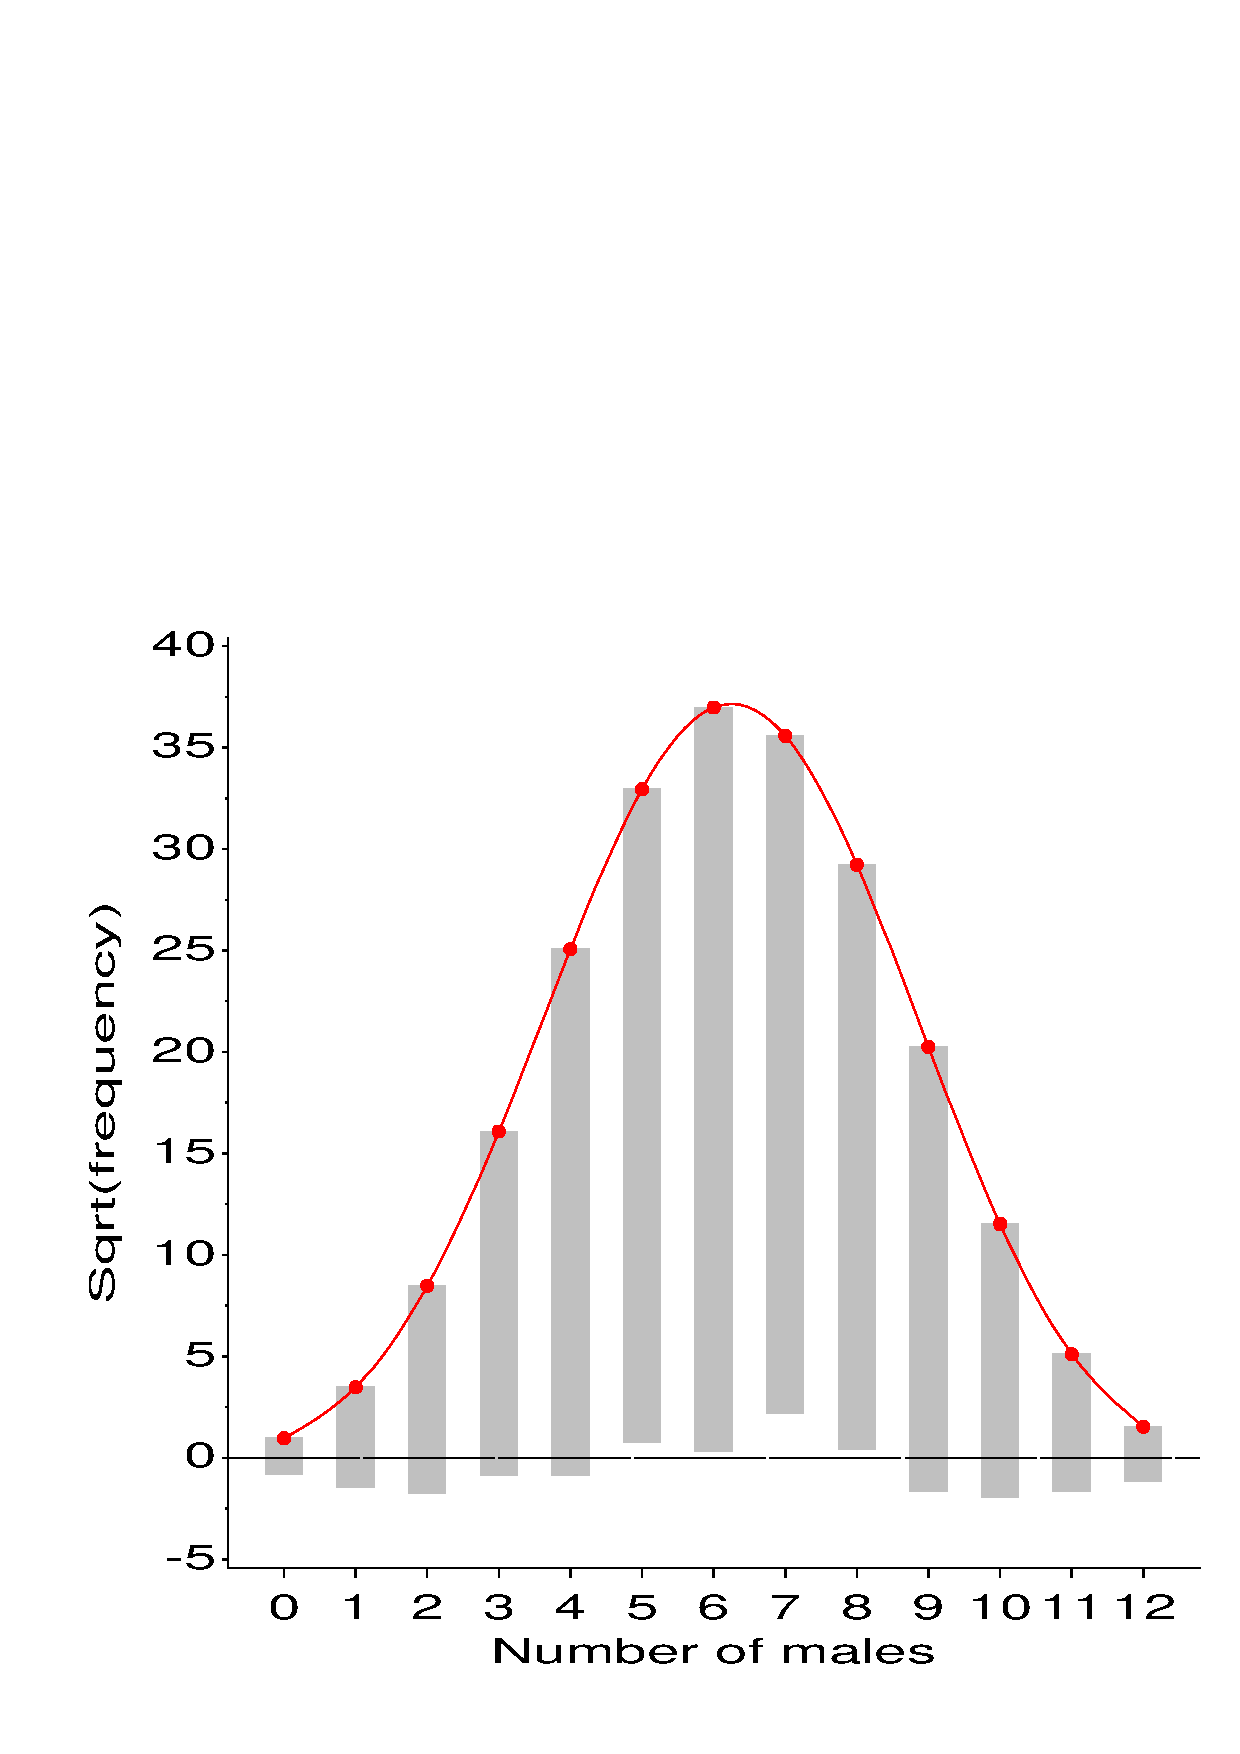
\includegraphics[scale=.5]{saxony}\graphicsfile{ch2/fig/saxony.eps}{}
  \caption[Hanging rootogram for Saxony families, Binomial model]{Hanging rootogram for Saxony families, Binomial($12, p$) model.
The systematic pattern of deviations shows that the Binomial model is not completely adequate for these data.}\label{fig:saxony}
\end{figure}
\end{Example}


\subsection{Maximum likelihood estimation}
\secref{sec:discrete-distrib} described the common discrete distributions,
their probability functions, and sample estimates.
Here we consider the general case.
Suppose we have a multinomial sample of
$K$ ``groups'', with frequencies of $n_k$ in group
$k$, and $\sum_k n_k = N$.
Suppose further that we have a probability model which specifies
the probability, \( \pi_k (\vec{\theta}), \: k = 1, 2, \dots ,  K \),
of an observation in group $k$, where $\vec{\theta}$ is a vector
of $s \geq 0$ parameters of the distribution
and $\sum_k \pi_k (\vec{\theta}) = 1$.

The likelihood, $\mathcal{L}$, is the probability of the data as
a function of the parameters,

\begin{equation*}
  \mathcal{L}(\vec{\theta}) = n ! \prod_{k=1}^K \frac{\pi_k (\vec{\theta})^{n_k}}{n_k !}
\end{equation*}

We can determine the value(s) of $\vec{\theta}$ which maximize $\mathcal{L}$
by maximizing the log-likelihood,

\begin{equation}\label{eq:loglikelihood}
 \ell(\vec{\theta}) \equiv
 \log \mathcal{L}(\vec{\theta}) = \log n ! +
  \sum_{k=1}^K n_k \log \pi_k (\vec{\theta}) - \sum_{k=1}^K \log n_k !
\end{equation}
The maximum likelihood estimate (MLE) of $\vec{\theta}$ will be
the value $\hat{\vec{\theta}}$ which is the solution of the
estimating equations
\begin{equation*}
\frac{\partial \log \mathcal{L}(\vec{\theta})}{\partial \vec{\theta}_i} = 0
\quad\quad i=1, 2, \dots s
\end{equation*}

For example, for the geometric distribution with probability
function \eqref{eq:geomf}, the log-likelihood is
\begin{equation*}
 \ell(\vec{\theta})   = n \log \theta +
  \sum_{k=1}^K (n_k - 1) \log (1-\theta)
\end{equation*}
which gives the estimating equation,
\begin{equation*}
\frac{\partial \ell(\theta)}{\partial \theta} =
\frac{(\sum_k n_k) - n}{1-\theta} + \frac{n}{\theta} = 0
\end{equation*}
whose solution is $\hat{\theta} = 1/\bar{k}$.  The fitted probabilities
under the geometric model
are then $\pi_k (\hat{\theta}) = (1 - \hat{\theta})^{k-1} \hat{\theta}$.

Having found the maximum likelihood estimate of the parameters, the
likelihood ratio
goodness-of-fit \GSQ{} statistic compares the maximized value of the
log-likelihood to the maximized log-likelihood of an unrestricted model
where the probabilities are only constrained so that $\sum_k \pi_k =1$.
In this case, there are $s=0$ parameters, and we symbolize the log-likelihood
by $ \ell(\theta_0) \equiv \ell(\vec{\pi})$.  For a multinomial sample this is

\begin{equation}\label{eq:loglikelihood0}
 \ell(\vec{\theta}_0)  = \log n ! +
  \sum_{k=1}^K n_k \log \pi_k  - \sum_{k=1}^K \log n_k !
\end{equation}
Maximizing \eqref{eq:loglikelihood0} subject to $\sum_k \pi_k =1$
gives $\hat{\pi}_k = n_k / N$.
The likelihood ratio statistic is

\begin{equation}\label{eq:likeratio}
 G^2 = -2 \log \left[
 \frac{\mathcal{L}(\vec{\theta}_0)}{\mathcal{L}(\vec{\theta})}
 \right]
 = 2 [ \ell(\vec{\theta}) - \ell(\vec{\theta}_0) ]
 = 2 \sum_{k=1}^{K} n_k \log \left( \frac{n_k}{N \pi_k (\hat{\theta}) } \right)
\end{equation}
which follows an asymptotic chi-square distribution with $K-1-s$ degrees
of freedom.


\subsection{Fitting discrete distributions as \loglin\ models}
In \secref{sec:pwrseries}, I described how the common discrete distributions
are all members of the general power series family.
Another general family of distributions---the exponential family---%
includes most of the common continuous distributions:
the normal, gamma, exponential, and others,
and is the basis of the class of generalized linear models fit
by \PROC{GENMOD}.

\citet{LindseyMersch:92}, \citet[6.1]{Lindsey:95} have shown how various discrete
(and continuous)
distributions can be fit to frequency data using Poisson \loglin{} models
available in \PROC{GENMOD}.  The uniform, geometric, binomial, and the
Poisson distributions may all be fit easily in this way.
A clear advantage is that this method gives estimated standard errors for the
distribution parameters as well as estimated confidence intervals
for fitted probabilities.

The essential idea is that, for frequency data, any distribution in the
exponential family may be represented by a linear model for the logarithm
of the cell frequency, with a Poisson distribution for errors,
otherwise known as a ``Poisson \loglin\ regression model''.
These have the form
\begin{equation*}
\log (N \pi_k) = \textrm{ offset } + \beta_0 + \vec{\beta}\trans \vec{S}(k)
 \comma
\end{equation*}
where $\vec{S}(k)$ is a vector of zero or more sufficient statistics for the
canonical parameters of the exponential family distribution,
and the offset term is a value which does not depend on the
parameters.  \tabref{tab:expfamily} shows the sufficient statistics and
offsets for several discrete distributions.
See \citet{LindseyMersch:92} for further details, and definitions
for the double-binomial distribution.

\input{ch2/tab/expfamily}

\begin{Example}[saxony2]{Families in Saxony}
The binomial distribution and the double binomial can both be fit to frequency data as a Poisson
regression using $\log \binom{n}{k}$ as an offset.
We only display results for the binomial model.
\begin{listing}
*-- calculate offset variables for binomial and double binomial;
data saxony;
   set saxony;
   logkn = log( gamma(12+1) / (gamma(males+1) * gamma(12-males+1)) );
   if 0 < males < 12
      then ylogity = -males * log(males/(12-males));
      else ylogity = 0;

   *-- fit binomial (12,p);
proc genmod data=saxony;
   model families = males /
      dist=poisson offset=logkn obstats ;

   *-- fit double binomial (12,p, psi);
proc genmod data=saxony;
   model families = males ylogity /
      dist=poisson offset=logkn obstats ;
\end{listing}
The goodness of fit tests shown in \outref{out:saxony2.1}
are equivalent to those calculated directly by the
\macro{GOODFIT} in \outref{out:saxony.2}.
The parameter estimate for \texttt{MALES}, $\beta_1 = 0.0769$
is actually estimating the logit of $p$, $\log p / (1-p)$,
so the inverse transformation gives
$\hat{p} = \frac{\exp (\beta_1)}{1 + \exp (\beta_1)} = 0.5192$,
as we had before.
The fitted frequencies (shown in \outref{out:saxony2.2}), given by the \opt{OBSTATS}{GENMOD}
on the \stmt{MODEL}{GENMOD} are the same as those
in \outref{out:saxony.1}.
The standard error for \texttt{MALES}, $s_{\beta_1} = 0.0074$
could also be transformed back to the probability scale in the same
way.
\begin{Output}
\caption{Fit of the Binomial($12, p$) to the Families in Saxony data: Goodness of fit tests}\label{out:saxony2.1}
\small
\verbatiminput{ch2/out/saxony2.1}
\end{Output}
\begin{Output}
\caption{Fit of the Binomial($12, p$) to the Families in Saxony data: Observed and fitted frequencies}\label{out:saxony2.2}
\small
\verbatiminput{ch2/out/saxony2.2}
\end{Output}
\end{Example}



\section{Diagnosing discrete distributions: Ord plots}%
\label{sec:discrete-Ord}
\ix{Ord plot|(}
Ideally, the general form chosen for a discrete distribution should
be dictated by substantive knowledge of a plausible mechanism
for generating the data.
When such knowledge is lacking, however,
we may not know which distribution is most appropriate for
some particular set of data.
In these cases, the question is often turned around, so that we seek
a distribution that fits well, and then try to understand the mechanism
in terms of aspects of the underlying probability theory (independent trials,
rare events, waiting-time to an occurrence, and so forth).

Although it is possible to fit each of several possibilities,
the summary goodness-of-fit statistics can easily be influenced by
one or two disparate cells, or additional (ignored or unknown) factors.
One simple alternative is a plot suggested by
\citet{Ord:67} which may be used to diagnose
the form of the discrete distribution.  Ord showed that a linear
relationship of the form,
\begin{equation} \label{eq:ord}
  \frac{ k \,  p(k) } { p(k-1) }
 = a  +  b \,  k \comma
\end{equation}
holds for each of the Poisson, binomial, negative binomial, and
logarithmic series distributions, and these distributions are
distinguished by the signs of the intercept,
$a$, and slope, $b$, as shown in
\tabref{tab:ordparm}.
The slope, \(b\),
in \eqref{eq:ord} is zero for the
Poisson, negative for the binomial, and positive for the negative
binomial and logarithmic series distributions; the latter two are
distinguished by their intercepts.
\ix{Poisson distribution}
\ix{logarithmic series distribution}
\ix{binomial distribution}
\ix{negative binomial distribution}

Thus, a plot of \(k \,  n_k /  n_{k-1}\) against \(k\), if linear,
is suggested as a means to determine which of these distributions to apply.
The values of the slope and intercept provide rough estimates of the
distribution parameters.

\begin{table}[htb]
\caption[Diagnostic slope and intercept for four discrete distributions]{Diagnostic slope and
intercept for four discrete distributions.  The ratios $k n_k / n_{k-1}$ plotted
against $k$ should appear as a straight line, whose slope and intercept
determine the particular distribution.}
\label{tab:ordparm}
\begin{center}
%\vspace{1ex}
\begin{tabular}{|ccll|}\hline
Slope & Intercept & Distribution & Parameter \\
(b)   & (a)       & (parameter)  &  estimate \\ \hline
0     &  $+$      &  Poisson (\(\lambda\)) & \(\lambda = a\)    \\
$-$   &  $+$      &  Binomial (n, p)       & \(p = b / (b-1)\)  \\
$+$   &  $+$      &  Negative binomial (n,p)      & \(p = 1 - b\)      \\
$+$   &  $-$      &  Log.\ series (\(\theta\)) & \(\theta =  b\) \\
      &      &                     &   \(\theta = - a\) \\ \hline
\end{tabular}
\end{center}
\end{table}

\subsubsection{Fitting the line}
One difficulty in applying this technique is that the number of points
(distinct values of $k$)
in the Ord plot is often small, and the sampling variances of
\(k \,  n_k /  n_{k-1}\) can vary enormously.
A little reflection indicates that points where $n_k$ is small
should be given less weight in determining the slope of the
line (and hence determining the form of the distribution).
In the small number of cases I've
tried, I have found that using a weighted least squares fit of \(k \,
n_k /  n_{k-1}\) on \(k\), using weights of \(w_k = \sqrt { n_k -1
}\)
produces reasonably good%
\footnote{This definition implies that frequencies of $n_k =1$
are ignored in fitting the line.}
automatic diagnosis of the form of a
probability distribution, but this choice is surely open to further study.

\subsubsection{Examples}
\begin{Example}[horskick3]{Death by horse kick}
The table below shows the calculations for
the horse kicks data, with the ratio \({ k \,  n_k } /  { n_{k-1}
}\) labeled \texttt{y}.  The weighted least squares line, with weights
\(w_k\), has a slope close to zero, indicating the Poisson
distribution.  The estimate \(\lambda = a = .656\) compares
favorably with the MLE, $\lambda=0.610$ and the
value from the Poissonness plot, shown in the
following section.
\ixd{death by horse kick}

\begin{alltt}
      Ord Plot: Deaths by Horsekicks

   k     \(n\sb{k}\)    \(n\sb{k-1}\)       \(w\sb{k}\)         y

   0    109      .    10.3923     .        -- Weighted LS --
   1     65    109     8.0000    0.5963    slope = -0.034
   2     22     65     4.5826    0.6769    inter = 0.656
   3      3     22     1.4142    0.4091
   4      1      3     0.0000    1.3333
\end{alltt}
\end{Example}

\begin{Example}[madison3]{Federalist papers}
For the word frequency data, the slope is positive, so either the
negative binomial or log series are possible.  The intercept is
essentially zero, which is ambiguous.  However, the logarithmic
series requires \(b \approx  - a\), so the negative binomial is a
better choice.  Mosteller \& Wallace did in fact find a reasonably
good fit to this distribution.
\ix{logarithmic series distribution}
\ix{negative binomial distribution}
\ixd{Federalist papers}

\begin{alltt}
      Instances of 'may' in Federalist papers

   k     \(n\sb{k}\)    \(n\sb{k-1}\)       \(w\sb{k}\)         y

   0    156      .    12.4499     .       -- Weighted LS --
   1     63    156     7.8740    0.4038   slope = 0.424
   2     29     63     5.2915    0.9206   inter = -0.023
   3      8     29     2.6458    0.8276
   4      4      8     1.7321    2.0000
   5      1      4     0.0000    1.2500
   6      1      1     0.0000    6.0000
\end{alltt}

Plots of data fitting four different discrete distributions are
shown in \figref{fig:orddemo}, using the data previously examined
in this chapter.
In each case, the slope and intercept of the weighted least squares line correctly
identify the distribution.
\end{Example}

\subsubsection{Drawbacks}
Using a single plot to determine one of four common discrete
distributions is advantageous, but our enthusiasm should be
limited by several weaknesses:

\begin{itemize*}
\item The Ord plot lacks resistance, since a single discrepant
       frequency affects the points for both \(k\) and \(k  +  1\).

\item The sampling variance of \(k \,  n_k /  n_{k-1}\) fluctuates
       widely
       \citep{HoaglinTukey:85,JinkinsonSlater:81}.  The use of weights \(w_k\) helps, but is purely a
       heuristic device.
\end{itemize*}


\begin{figure}[htb]
 \begin{minipage}[b]{.5\linewidth}
  \centering
  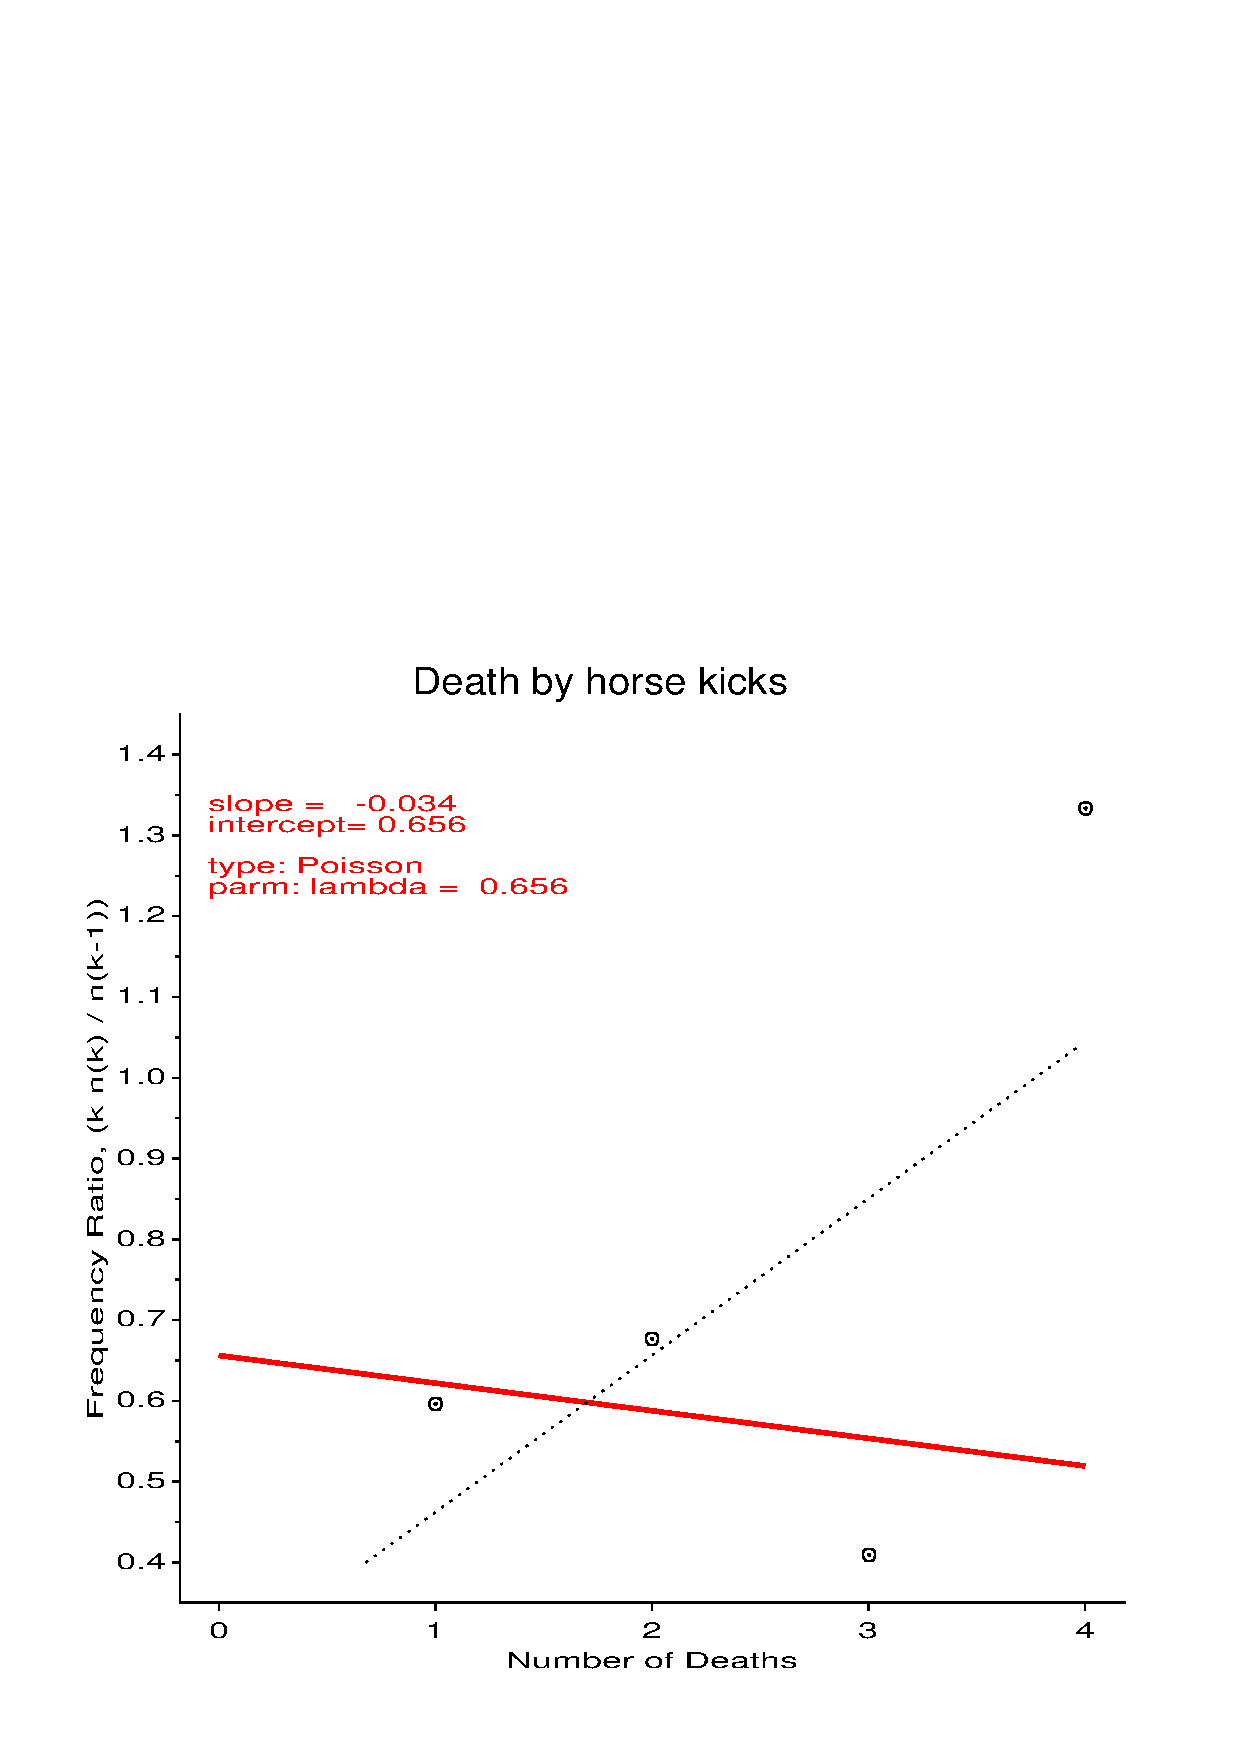
\includegraphics[width=.9\linewidth]{orddemo1}\graphicsfile{ch2/fig/orddemo1.eps}{}
 \end{minipage}%
 \begin{minipage}[b]{.5\linewidth}
  \centering
  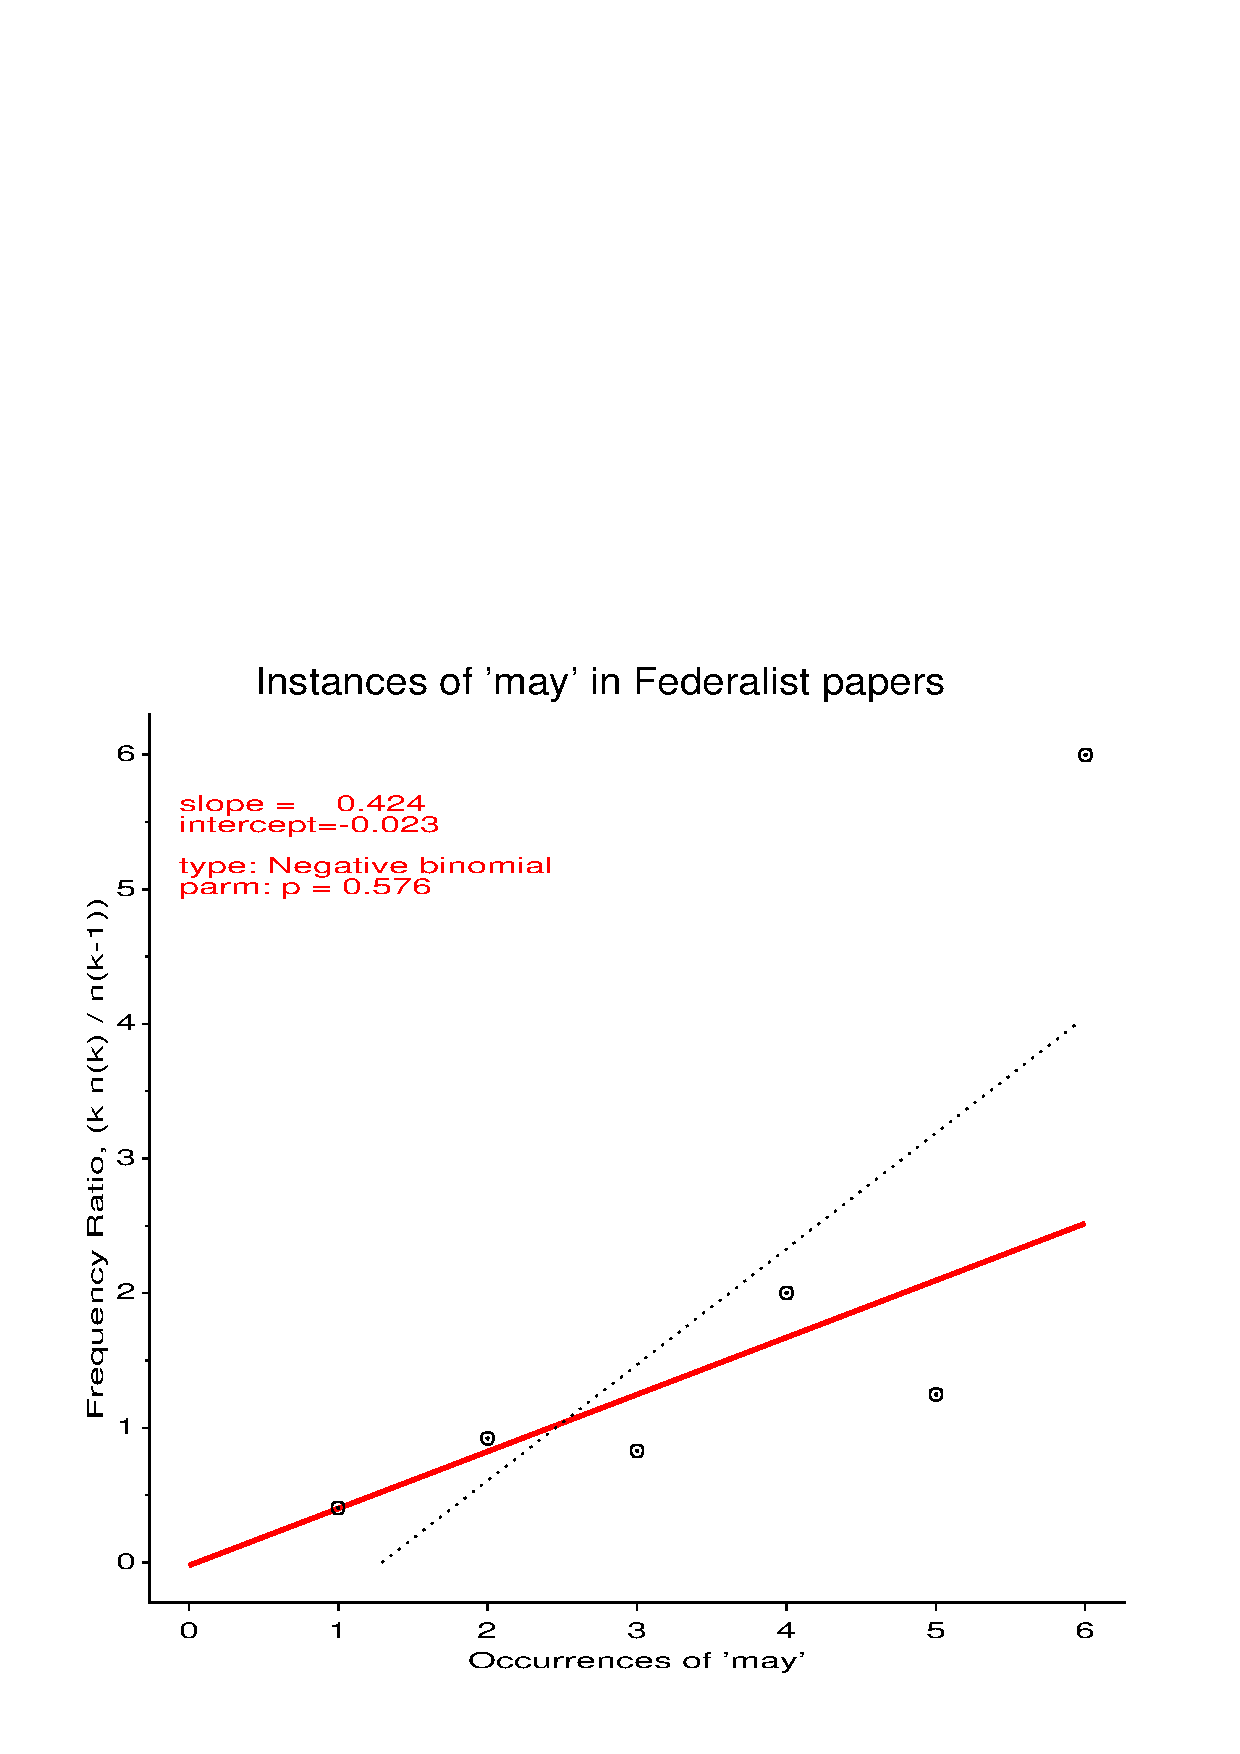
\includegraphics[width=.9\linewidth]{orddemo2}\graphicsfile{ch2/fig/orddemo2.eps}{}
 \end{minipage}
 \\[3ex]
 \begin{minipage}[b]{.5\linewidth}
  \centering
  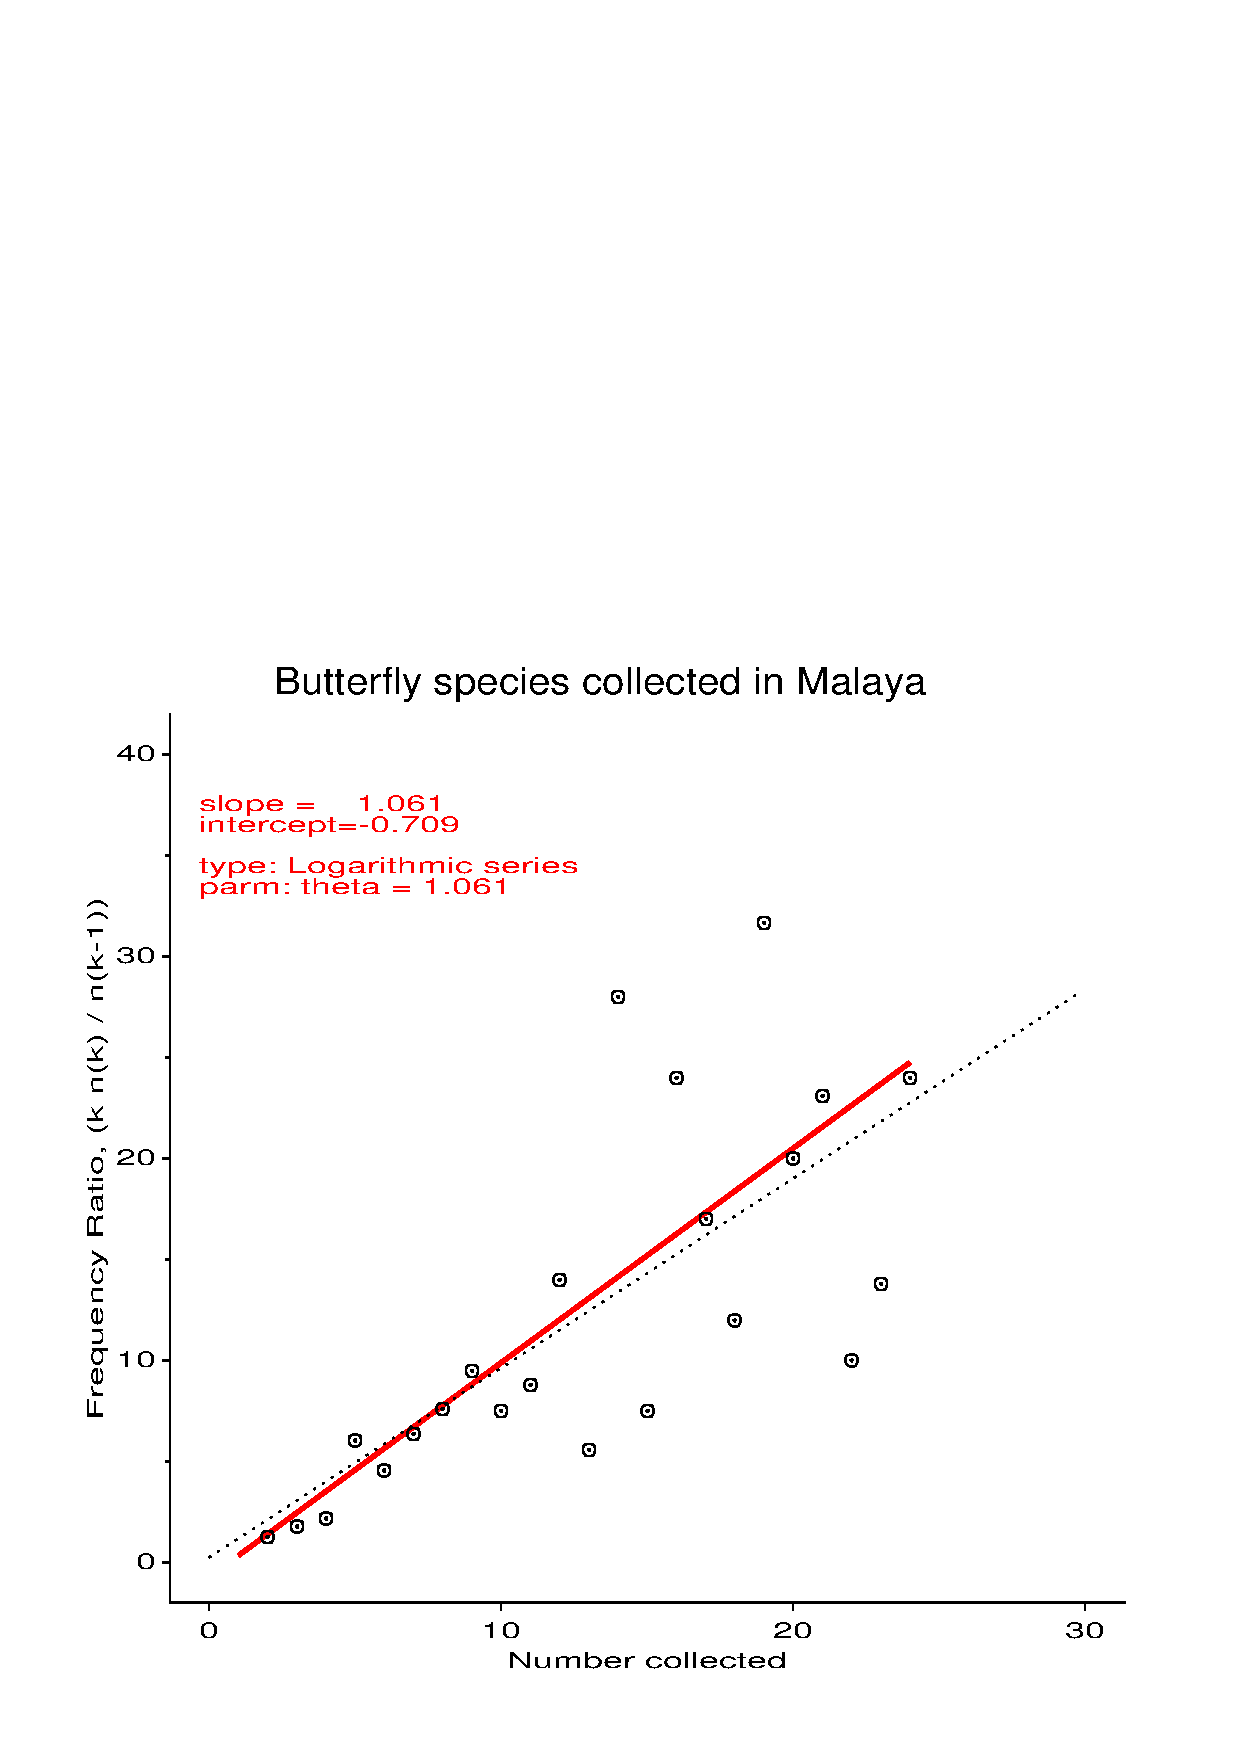
\includegraphics[width=.9\linewidth]{orddemo3}\graphicsfile{ch2/fig/orddemo3.eps}{}
 \end{minipage}%
 \begin{minipage}[b]{.5\linewidth}
  \centering
  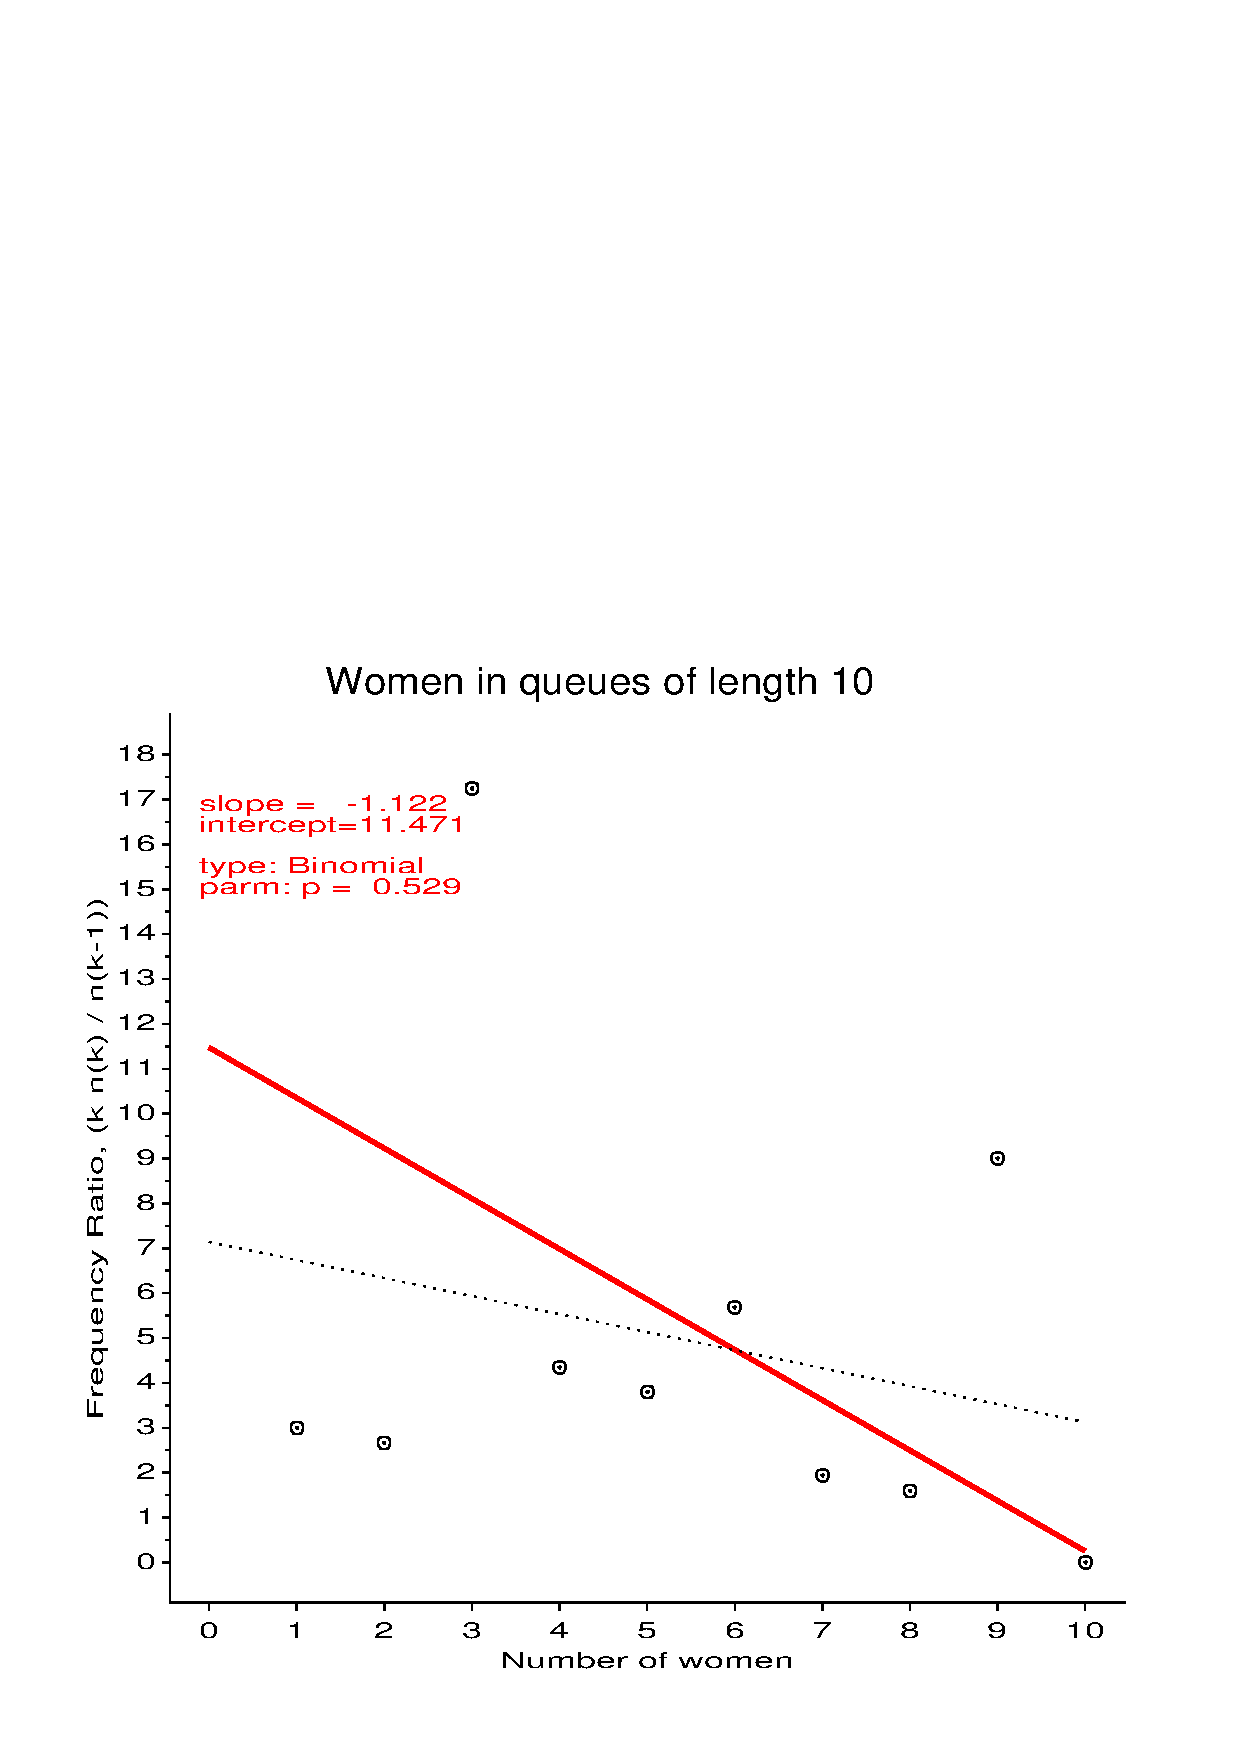
\includegraphics[width=.9\linewidth]{orddemo4}\graphicsfile{ch2/fig/orddemo4.eps}{}
 \end{minipage}
 \caption[Ord plots for four discrete distributions]{Ord plots for four discrete
distributions.  Each panel shows the least squares line (dotted, black) and the weighted least squares line (solid, red). The slope and intercept of the weighted least squares line are used to
identify the type of the distribution.}\label{fig:orddemo}
\end{figure}

\subsubsection{ORDPLOT macro}
These plots are produced by the \macro{ORDPLOT} (see \ref{mac:ordplot}).  For the horse kicks
data,  the plot in \figref{fig:orddemo} is produced with the macro call
\begin{listing}
%ordplot(data=horskick,
         count=Deaths, freq=corpsyrs);
\end{listing}
The \mparm{FREQ}{ORDPLOT} gives the name of the basic frequency variable ($k$),
and the \mparm{COUNT}{ORDPLOT} gives the associated count, $n_k$.
\ix{Ord plot|)}

\section{Poissonness plot}\label{sec:discrete-Poissonness}
\ix{Poissonness plot|(}

The Poissonness plot
\citep{Hoaglin:80}
is designed as a plot of some
quantity against \(k\), so that the result will be points along a
straight line when the data follow a \IX{Poisson distribution}.  When the
data deviate from a Poisson, the points will be curved.
\citet{HoaglinTukey:85}
develop similar plots for other discrete distributions,
including the binomial, negative binomial, and logarithmic series
distributions.
\ix{binomial distribution}
\ix{negative binomial distribution}

\subsection{Features of the Poissonness plot}
The Poissonness plot has the following desirable features:
\begin{itemize}
\item \boldital{Resistance}: a single discrepant value of \(n_k\)
       affects only the point at value \(k\).  (In the Ord plot
       it affects each of its neighbors.)
\item \boldital{Comparison standard}:  An approximate confidence
       interval can be found for each point, indicating its inherent
       variability and helping to judge whether each point is
       discrepant.
\item \boldital{Influence}:  Extensions of the method result in
       plots which show the effect of each point on the estimate of
       the main parameter of the distribution (\(\lambda\) in the
       Poisson).
\end{itemize}

\subsection{Plot construction}
Assume, for some fixed \(\lambda\), each observed frequency, \(n_k\)
equals the expected frequency, \(m_k = N p_k\).  Then, setting
\(n_k = N p_k  = N { e^{ - \lambda } \:  \lambda^k } /  { k ! }\),
and taking logs of both sides gives

\begin{equation*}
  \log ( n_k ) = \log \,  N - \lambda  +  k \,  \log \,  \lambda  -
  \log \,  k !
\end{equation*}
which can be rearranged to
\begin{equation} \label{eq:poispl}
  \log \left(  \frac{ k ! \:  n_k } {N} \right)
 = - \lambda  +  ( \log \,  \lambda ) \,  k
 \period
\end{equation}

The left side of \eqref{eq:poispl} is called the \glossterm{count metameter}, and
denoted \(\phi \,  ( n_k )  = \log_e ( k ! \,  n_k  /  N )\).  Hence,
plotting \(\phi ( n_k )\) against \(k\) should give a line
\(\phi ( n_k )= a + b k\) with

\begin{itemize*}
\item slope = \(\log  \,  \lambda\)
\item intercept = \(- \lambda\)
\end{itemize*}
when the observed frequencies follow a Poisson distribution.
If the points in this plot are close enough to a straight line,
then an estimate of $\lambda$ may be obtained from the slope $b$ of the line,
$\hat{\lambda} = e^b$ should be reasonably close in value
to the MLE of $\lambda$, $\hat{\lambda} = \bar{x}$.
In this case, we might as well use the MLE as our estimate.

\subsubsection{Leveled plot}
If we have a preliminary estimate $\lambda_0$ of $\lambda$,
we can use this to give a new plot where the reference line
is horizontal, making comparison of the points with the line
easier.
In this leveled plot the vertical coordinate $\phi (n_k)$ is modified to
\begin{equation*}
 \phi ' (n_k) = \phi (n_k) + \lambda_0 - k \log \lambda_0
 \period
\end{equation*}
When the data follow a Poisson distribution with parameter
$\lambda$, the modified plot will have
\begin{itemize*}
\item slope = \(\log  \lambda - \log  \lambda_0 = \log ( \lambda / \lambda_0 ) \)
\item intercept = \(\lambda_0 - \lambda\)
\end{itemize*}
In the ideal case, where our estimate of $\lambda_0$ is close to the true
$\lambda$, the line will be horizontal at $\phi ' = 0$.
The modified plot is particularly useful in conjunction with the
confidence intervals for individual points described below.

\subsubsection{Confidence intervals}
When one or two points deviate from an otherwise nearly linear
relation,
it is helpful to determine whether the discrepancy is consistent with
chance variation.
As well, we must recognize that classes with small frequencies $n_k$
are less precise than classes with large frequencies.
\citet{HoaglinTukey:85} develop approximate confidence intervals
for $\log m_k$ for each point in the Poissonness plot.
These are calculated as
\begin{equation*}
\phi \left( n_k^{*}\right) \pm h_k
\end{equation*}
where the count metameter function is calculated using a modified frequency $%
n_k^{*}$, defined as

\begin{equation*}
n_k^{*}= \left\{
\begin{array}{ll}
n_k-.8n_k-.67 & n\geq 2 \\
1/e & n=1 \\
\textrm{undefined} & n=0
\end{array}
\right.
\end{equation*}
%
and $h_k$ is the half-width of the 95\% confidence interval,
\begin{equation*}
h_k=1.96\frac{\sqrt{1-\widehat{p}_k}}{[n_k-(.25\widehat{p}_k+.47)\sqrt{n_k}%
]^{1/2}}
\end{equation*}
and $\hat{p}_k = n_k / N$.

\subsection{The \macro{POISPLOT}}
The \macro{POISPLOT} (see \macref{mac:poisplot}) performs the calculations and produces the
plots for all examples shown in this section.
The input data should contain a basic count variable (corresponding to $k$)
and a frequency variable (corresponding to $n_k$)
of the form shown in \tabref{tab:horskick}.

\begin{Example}[horskick2]{Death by horse kick}
A Poissonness plot is produced for the Horse kick data
using the \macro{POISPLOT} with
the following statements:
\begin{listing}
title 'Poissoness Plot: Deaths by Horsekicks' ;
data horskick;
    input deaths corpsyrs;
    label deaths='Number of Deaths'
       corpsyrs='Number of Corps-Years';
   datalines;
    0    109
    1     65
    2     22
    3      3
    4      1
;
%poisplot(data=horskick, count=Deaths,freq=corpsyrs);

\end{listing}

The calculations for the poissonness plot, including confidence
intervals, are shown below for the horse kicks data.  The macro
produces the plot in
\figref{fig:poisdemo1}.
The fitted least squares line has a slope of -0.431, which would
indicate $\lambda = e^{-0.431} = 0.65$.  This compares well with the MLE,
$\lambda = \bar{x} = 0.61$.
\ixd{death by horse kick}

\begin{alltt}
           \(\phi(n\sb{k})\)        CI       CI      Confidence Int
k    nk        Y       center   width     lower    upper

0   109   -0.607      -0.617    0.130    -0.748   -0.487
1    65   -1.124      -1.138    0.207    -1.345   -0.931
2    22   -1.514      -1.549    0.417    -1.966   -1.132
3     3   -2.408      -2.666    1.318    -3.984   -1.348
4     1   -2.120      -3.120    2.689    -5.809   -0.432
\end{alltt}
\begin{figure}[htb]
  \centering
  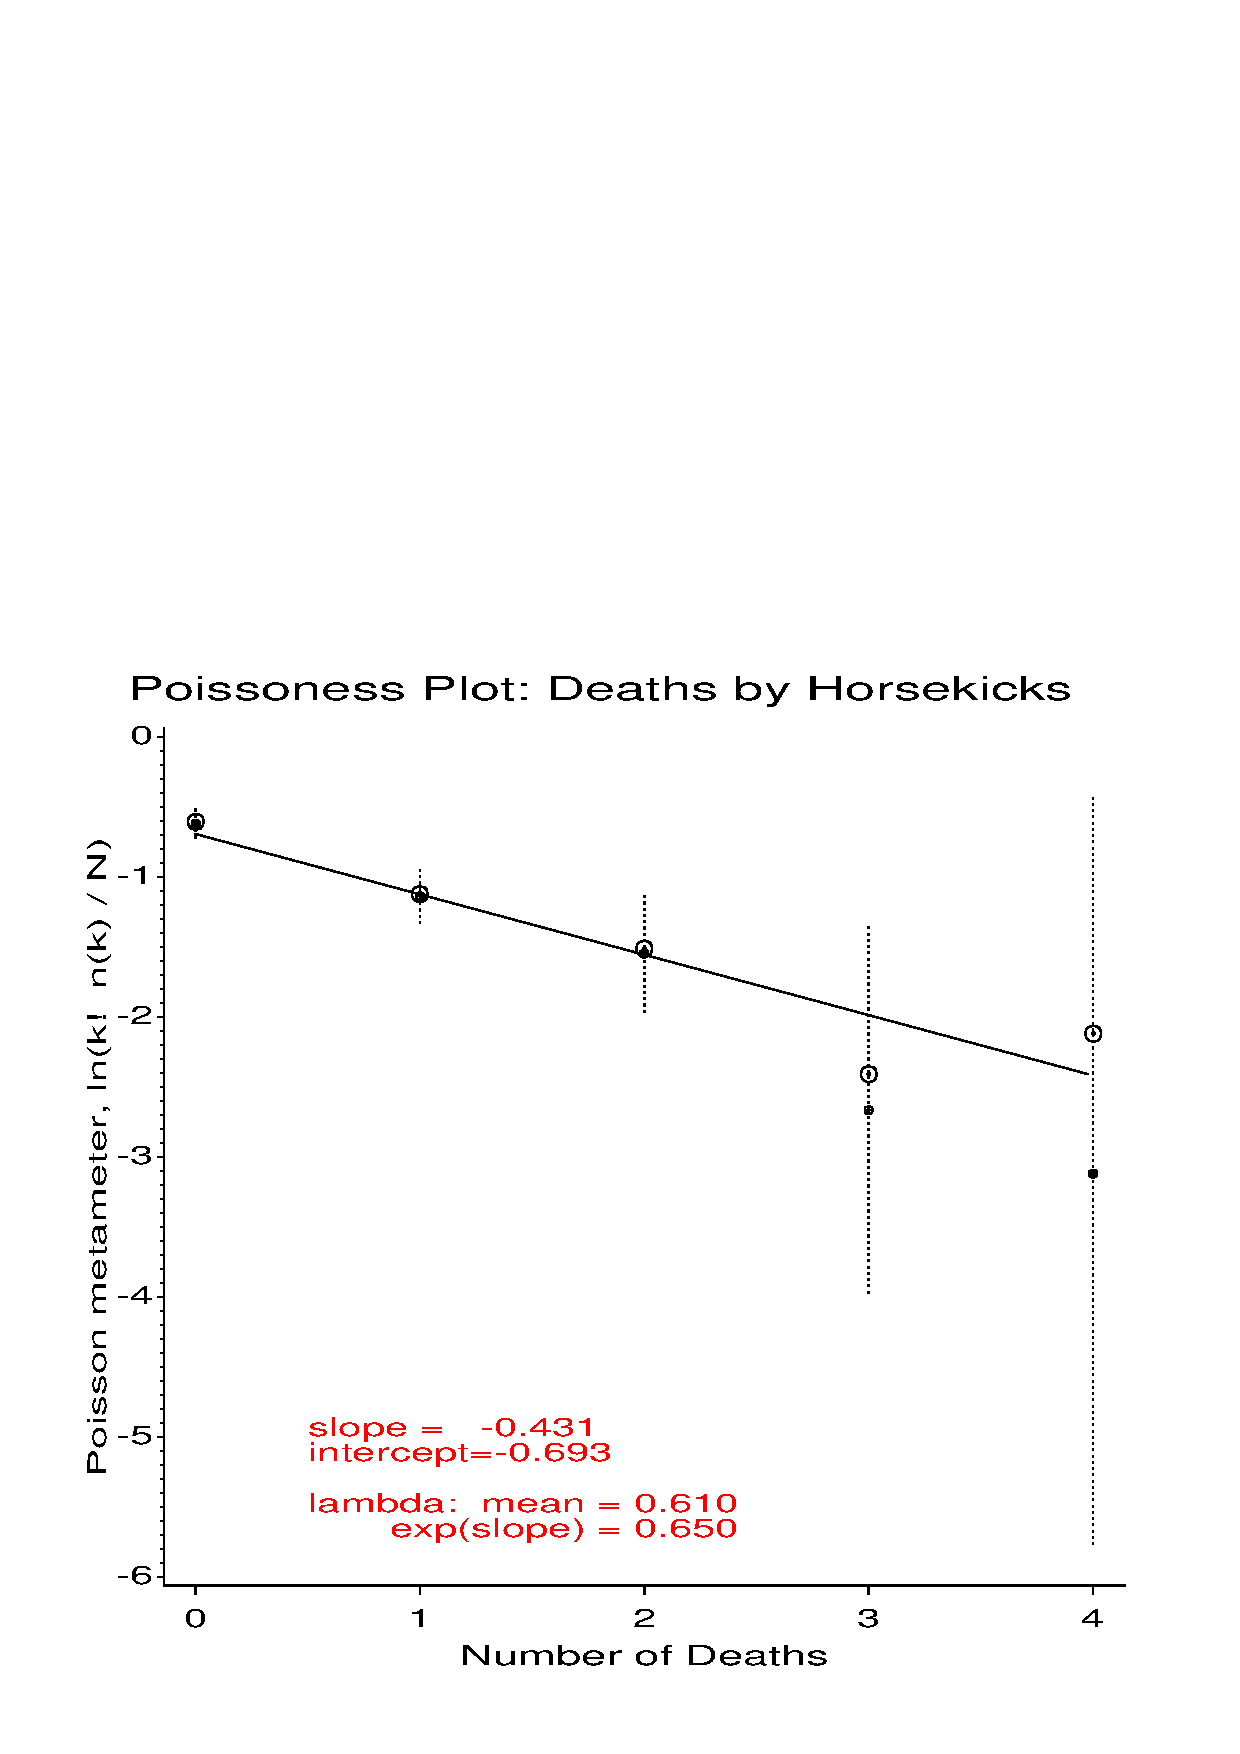
\includegraphics[scale=.5]{poisdemo1}\graphicsfile{ch2/fig/poisdemo1.eps}{}
  \caption[Poissonness plots for the horse kick data]{Poissonness plots
for the horse kick data.  The data fits the Poisson distribution
reasonably well.}\label{fig:poisdemo1}
\end{figure}

The leveled Poissonness plot (see \figref{fig:poisdemo2}) is produced by the \texttt{\%POISPLOT} statement
below, specifying \pname{LAMBDA=.610}.
%% input: /users/faculty/friendly/sasuser/catdata/poisdemo.sas
%% last modified: 08-Apr-99 12:38
\begin{listing}
title;
%poisplot(data=horskick, count=Deaths, freq=corpsyrs,
          lambda=.610, plot=dist);
run;
\end{listing}

\begin{figure}[htb]
  \centering
  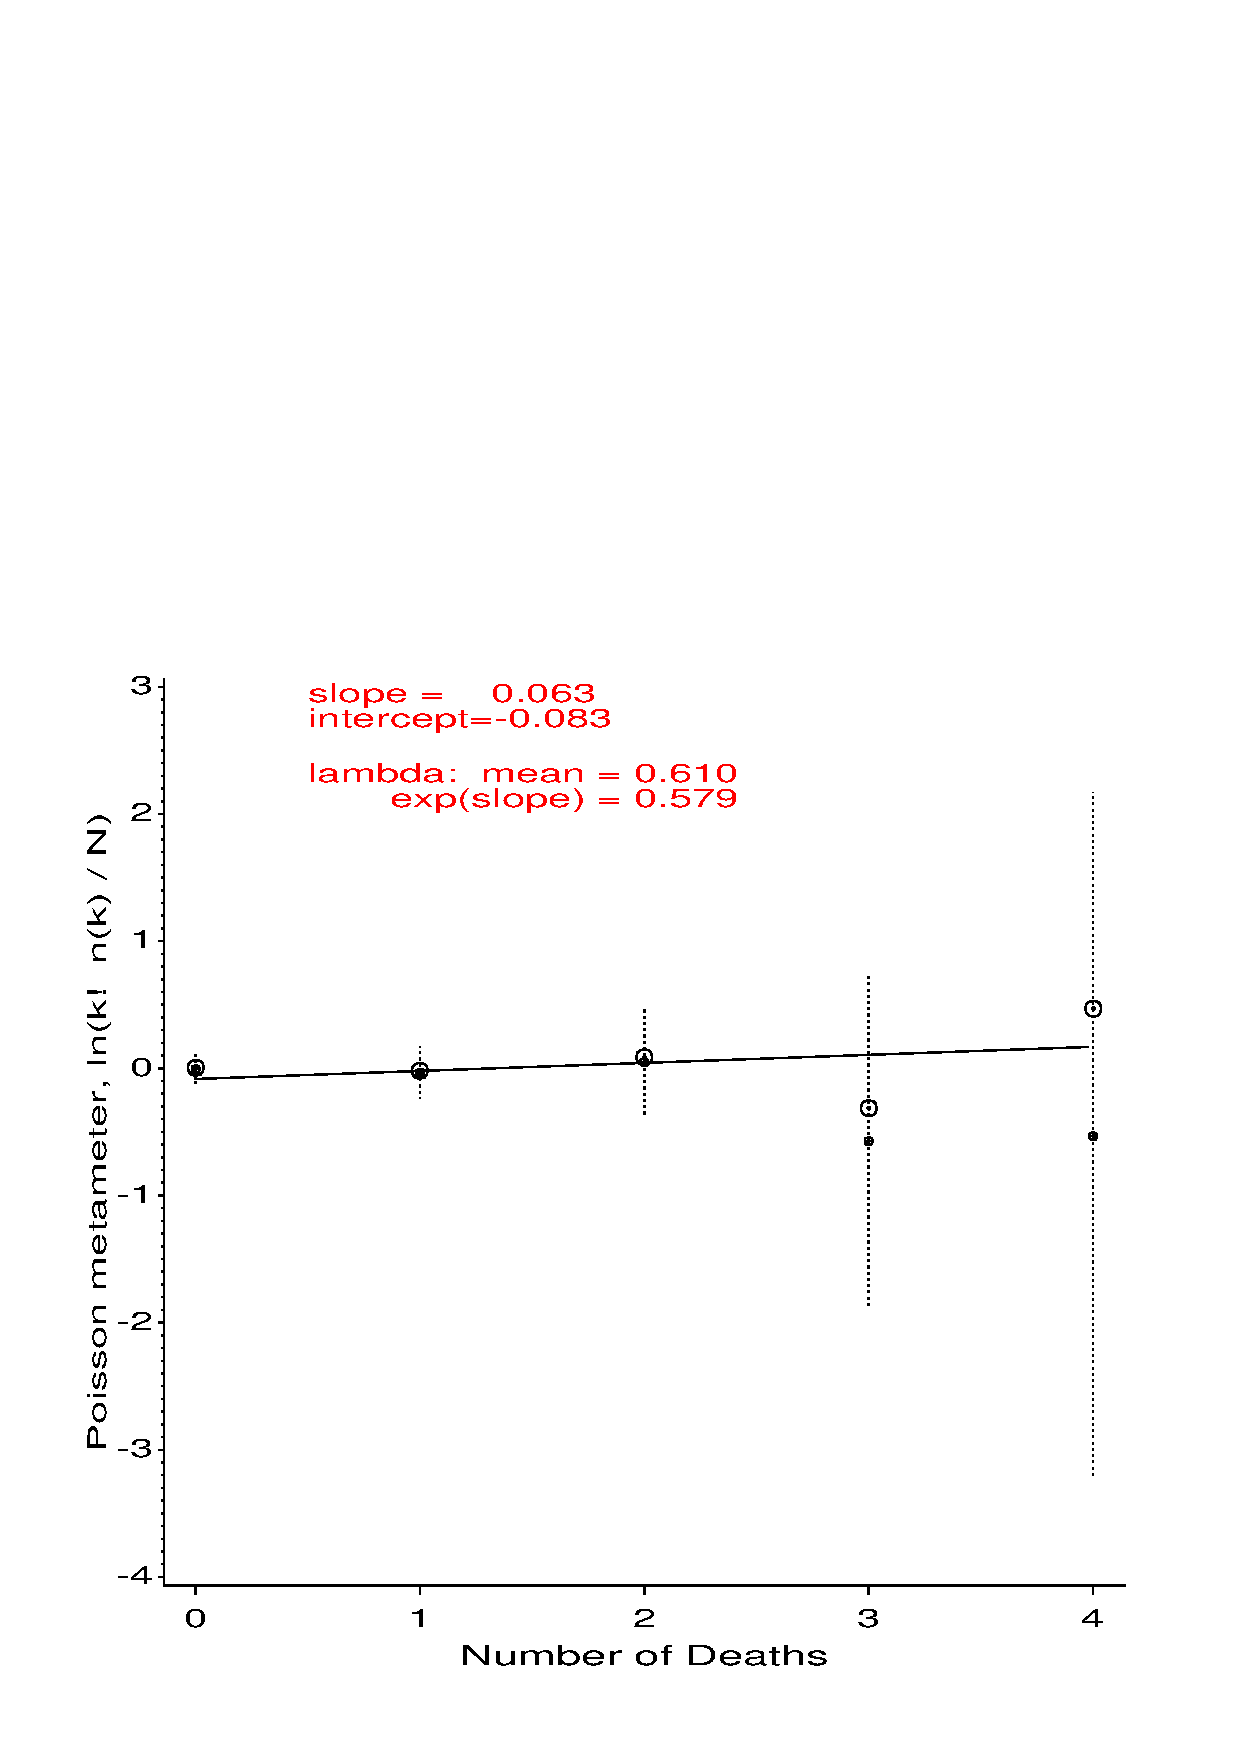
\includegraphics[scale=.5]{poisdemo2}\graphicsfile{ch2/fig/poisdemo2.eps}{}
  \caption[Leveled poissonness plot for the horse kick data]{Leveled poissonness plot for the horse kick data.}\label{fig:poisdemo2}
\end{figure}
In both plots the fitted line is within the confidence intervals;
the widths of the intervals for $k > 2$ are graphic reminders that these observations
have relatively low precision.

For comparison, \figref{fig:poismad1} shows the Poissonness plot
for the occurrences of \emph{may} in the
Federalist Papers (\tabref{tab:madison}).
The systematic curvature in the plot, judged relative to the confidence
intervals,
 indicates that these data do not follow a Poisson distribution.
\end{Example}

\begin{figure}[htb]
  \centering
  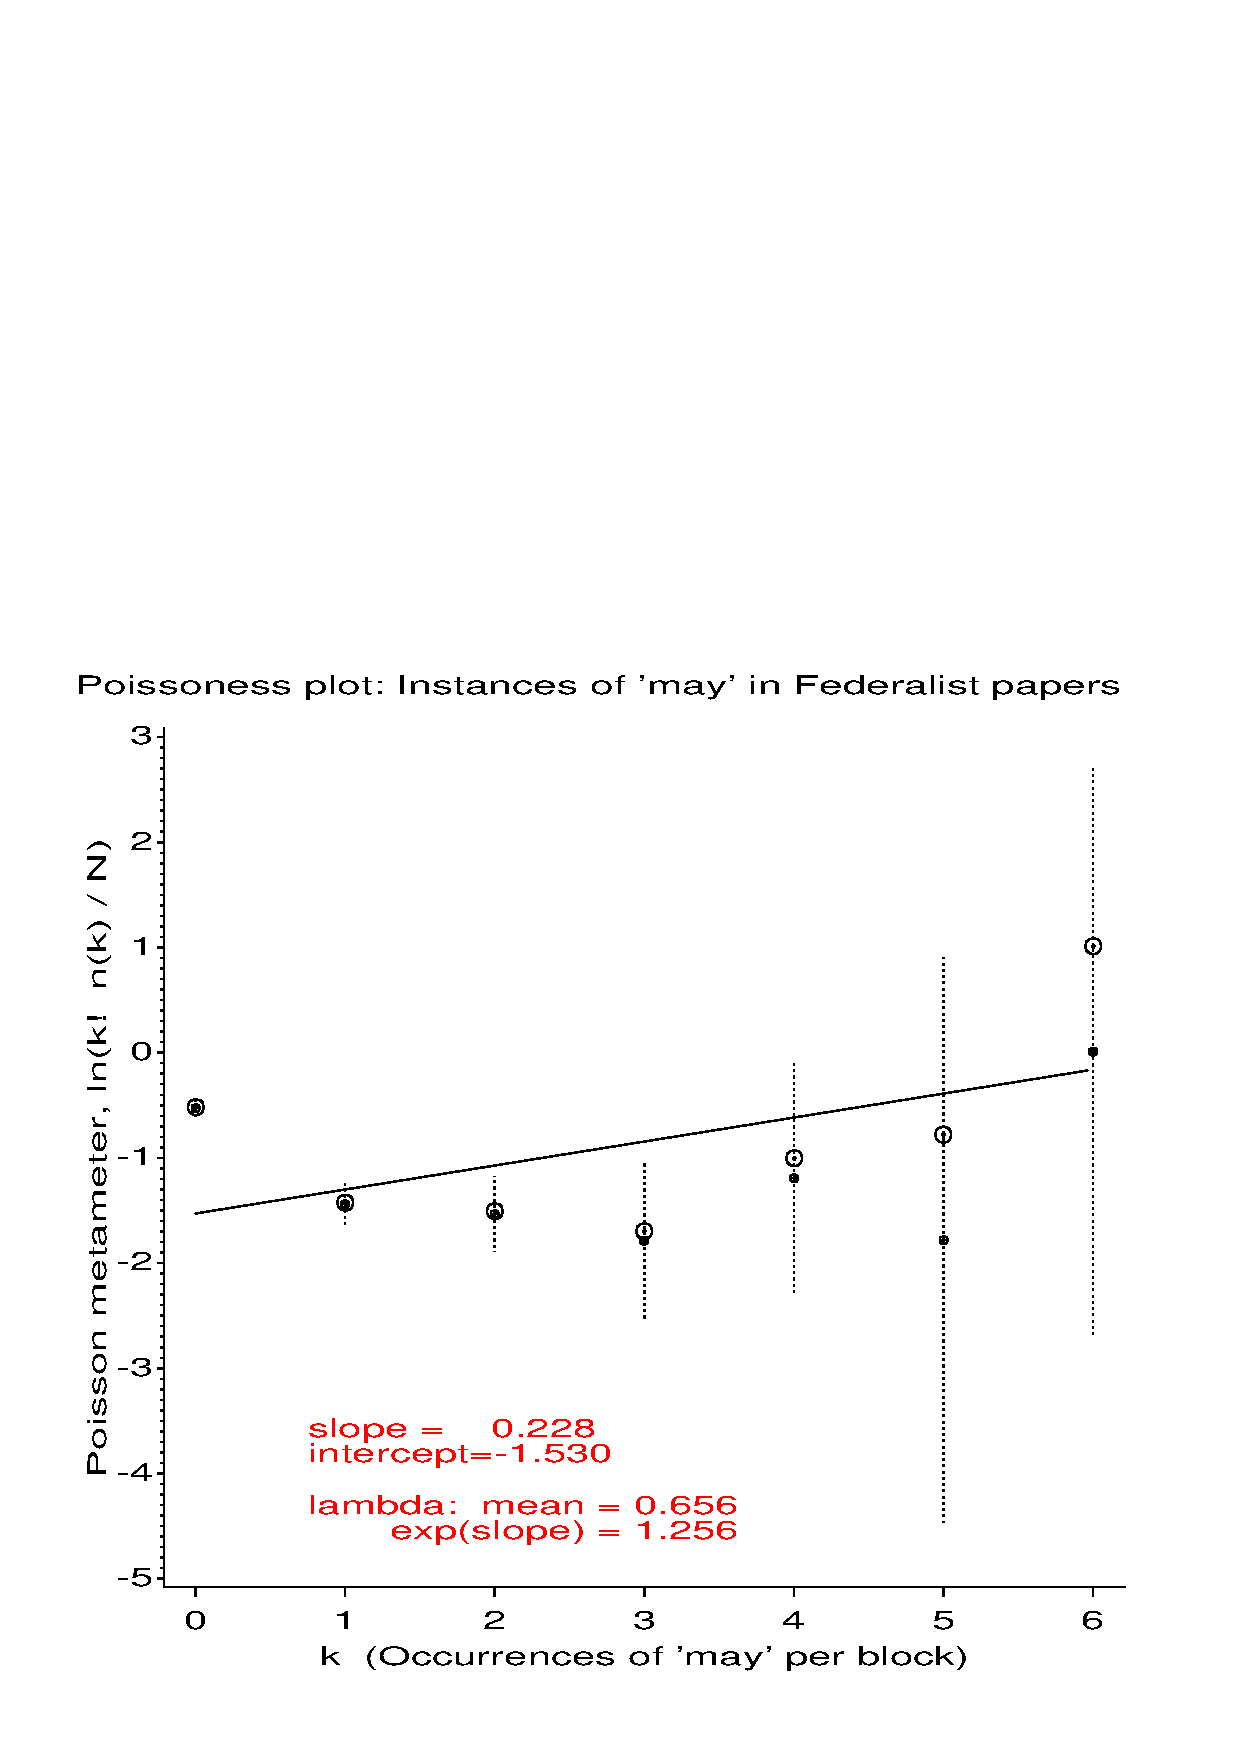
\includegraphics[scale=.5]{poismad1}\graphicsfile{ch2/fig/poismad1.eps}{}
  \caption[Poissonness plot for the Federalist Papers data]{Poissonness plot for the Federalist Papers data.
The systematic curvature in the plot indicates that this data does not follow a Poisson distribution.}\label{fig:poismad1}

\end{figure}
\subsection{Leverage and influence}
In standard models for quantitative data, common diagnostic techniques
attempt to estimate the effect that each observation has upon the
parameter estimates.
For linear models, these include measures of
\glossterm{leverage}---the potential
that an observation has to influence our results (due to its location
on the predictors),
and \glossterm{influence}---the actual effect this observation has
on parameter estimates and fitted values.

For discrete distributions, \citet{HoaglinTukey:85} derive
measures which are similar in spirit,  though based on the change in
the estimate of $ \lambda$ at each value of $k$ which would be
required to make the observed count metameter $\phi(n_k^{*})$
equal to its fitted value,
$\phi(m_k(\lambda_0))$ calculated using a contemplated or estimated $ \lambda_0$.

For the Poisson distribution, their analysis leads to the relation
\begin{equation}\label{eq:levpois}
\log \frac{\phi(n_k^{*})}{\phi(m_k(\lambda_0))}
= ( \lambda - \lambda_0 ) \left( \frac{k}{\lambda_0} - 1 \right)
\period
\end{equation}
Equation \eqref{eq:levpois} is 
a line through the origin with slope equal to $( \lambda - \lambda_0 )$.
By analogy with least squares regression through the origin
(where leverage is proportional to $x$), Hoaglin and Tukey
refer to $(k/\lambda_0) - 1$ as the leverage of point $k$.

Their parameter change plot shows each observation in the discrete
distribution as a point with vertical coordinate proportional to
$ \log [ \phi(n_k^{*}) / \phi(m_k(\lambda_0)) ] =
  \log ( \phi(n_k^{*})) - \log \phi(m_k(\lambda_0))$
and horizontal coordinate proportional to $k/\lambda_0 - 1$.
In this plot (see \figref{fig:poisdemo3}), the slope of
a line from the origin to a point shows the change in the Poisson
parameter, $\lambda - \lambda_0$ indicated by that
point.
The horizontal coordinate is proportional to the potential
of that observation to affect the Poisson parameter $\lambda$.

An alternative version of this plot, more in the spirit of the
influence plots for \loglin{} models and logistic regression
to be described later in this book, plots the
parameter change, $\lambda - \lambda_0$ directly on the
vertical axis against the same horizontal leverage value,
and uses a bubble whose size represents influence
as the plotting symbol.
%[More to be added here]

The parameter change plot and the influence plot are produced
with the \macro{POISPLOT} by including the keyword
\texttt{INFL} in the \texttt{PLOT=} parameter (i.e., \texttt{PLOT=DIST INFL}
gives all plots).
For the horse kick data, these plots are shown in
\figref{fig:poisdemo3} and \figref{fig:poisdemo4}.

\begin{figure}[htb]
  \centering
  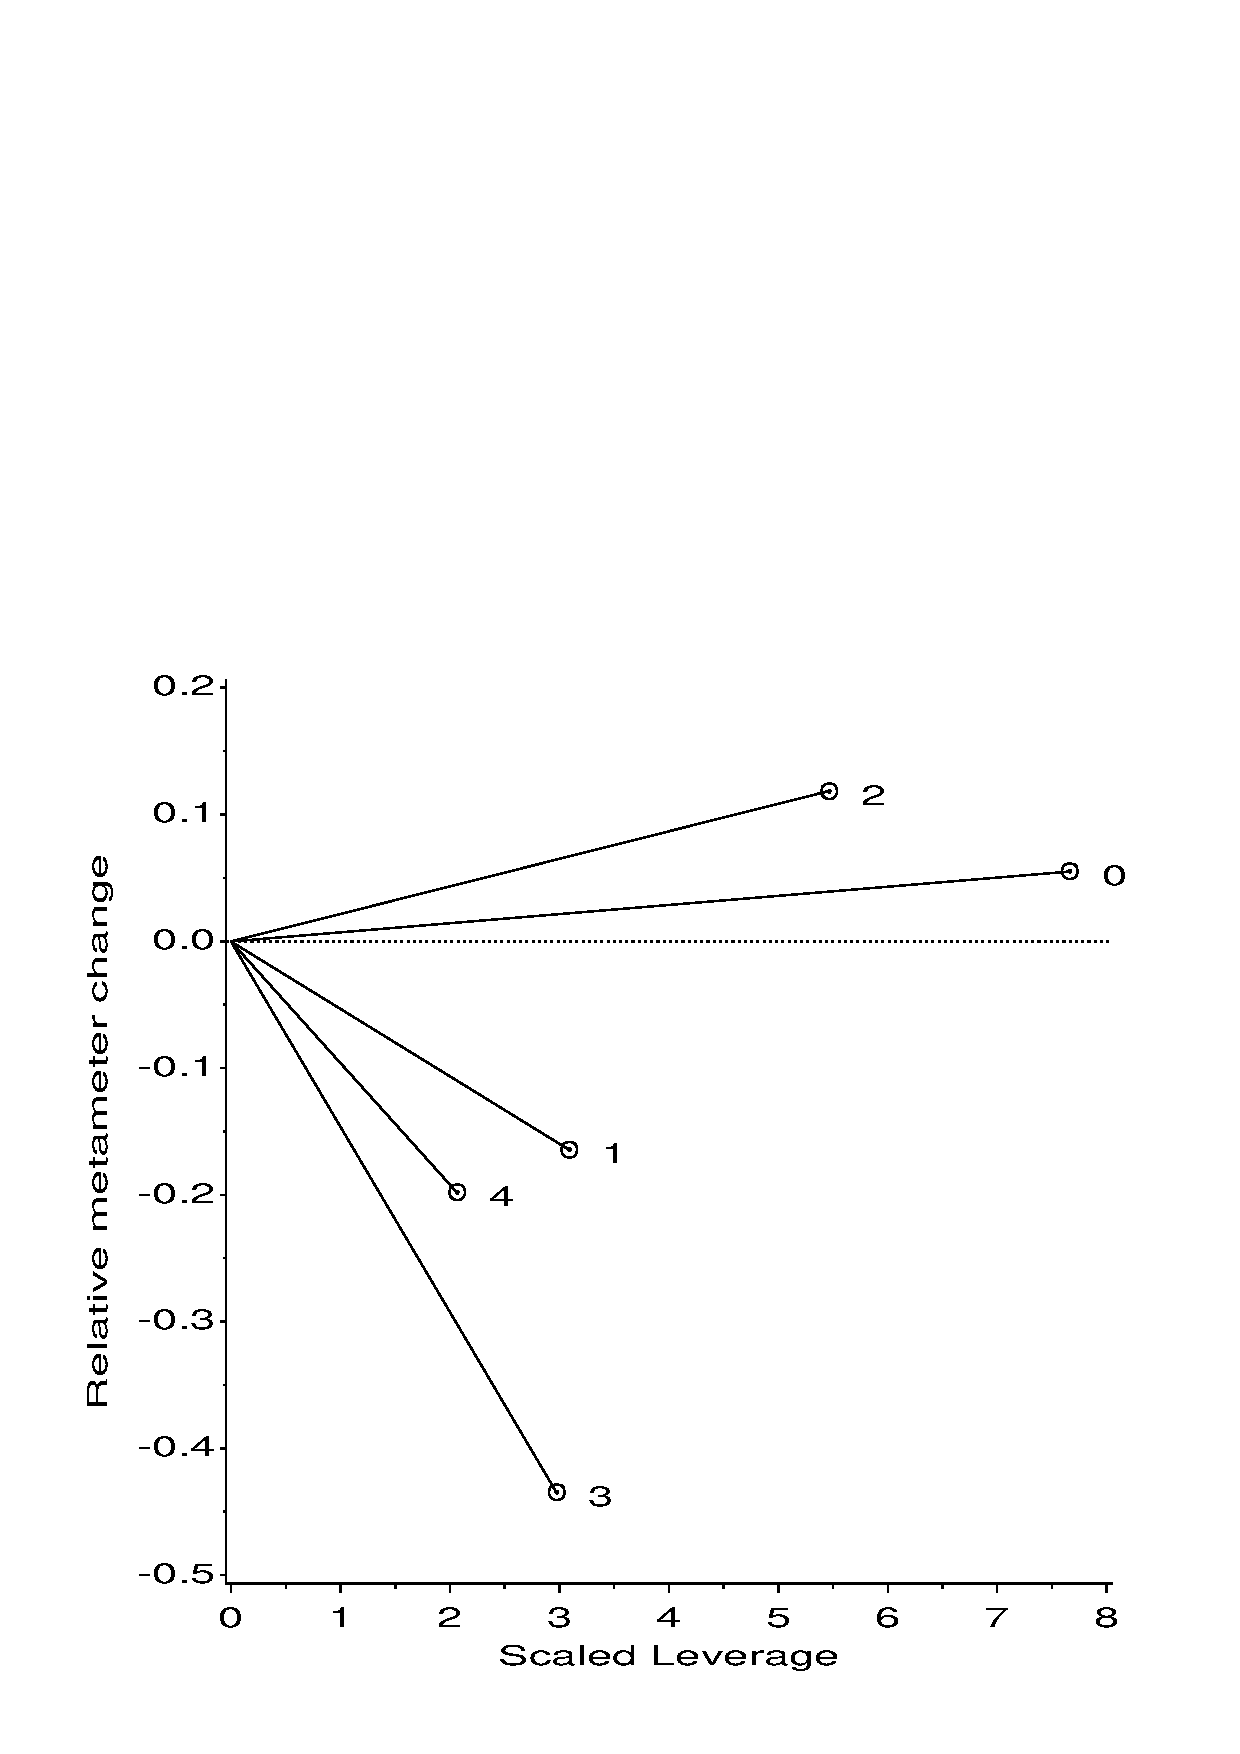
\includegraphics[scale=.5]{poisdemo3}\graphicsfile{ch2/fig/poisdemo3.eps}{}
  \caption[Parameter change plot for the Poisson parameter]{Parameter change
plot for the Poisson parameter, fitting the horse kick data.
The horizontal coordinate of each point is proportional to the potential of that observation to affect the value of $\lambda$.
The slope of the line through the origin is proportional to the
change in the count metameter.}\label{fig:poisdemo3}
\end{figure}
In \figref{fig:poisdemo3} we see that
the point corresponding to $k=0$ has the greatest leverage, but
influences $\lambda$ very little.
The point for $k=3$ has only moderate leverage, but has the greatest
impact on the Poisson parameter.
In \figref{fig:poisdemo2}
we see that the circle symbol for $\phi(n_k^{*})$
at $k=3$ is furthest from the
line.
\figref{fig:poisdemo4} shows that this point indicates a $\lambda$
value about 0.15 smaller than the estimated value.
\begin{figure}[htb]
  \centering
  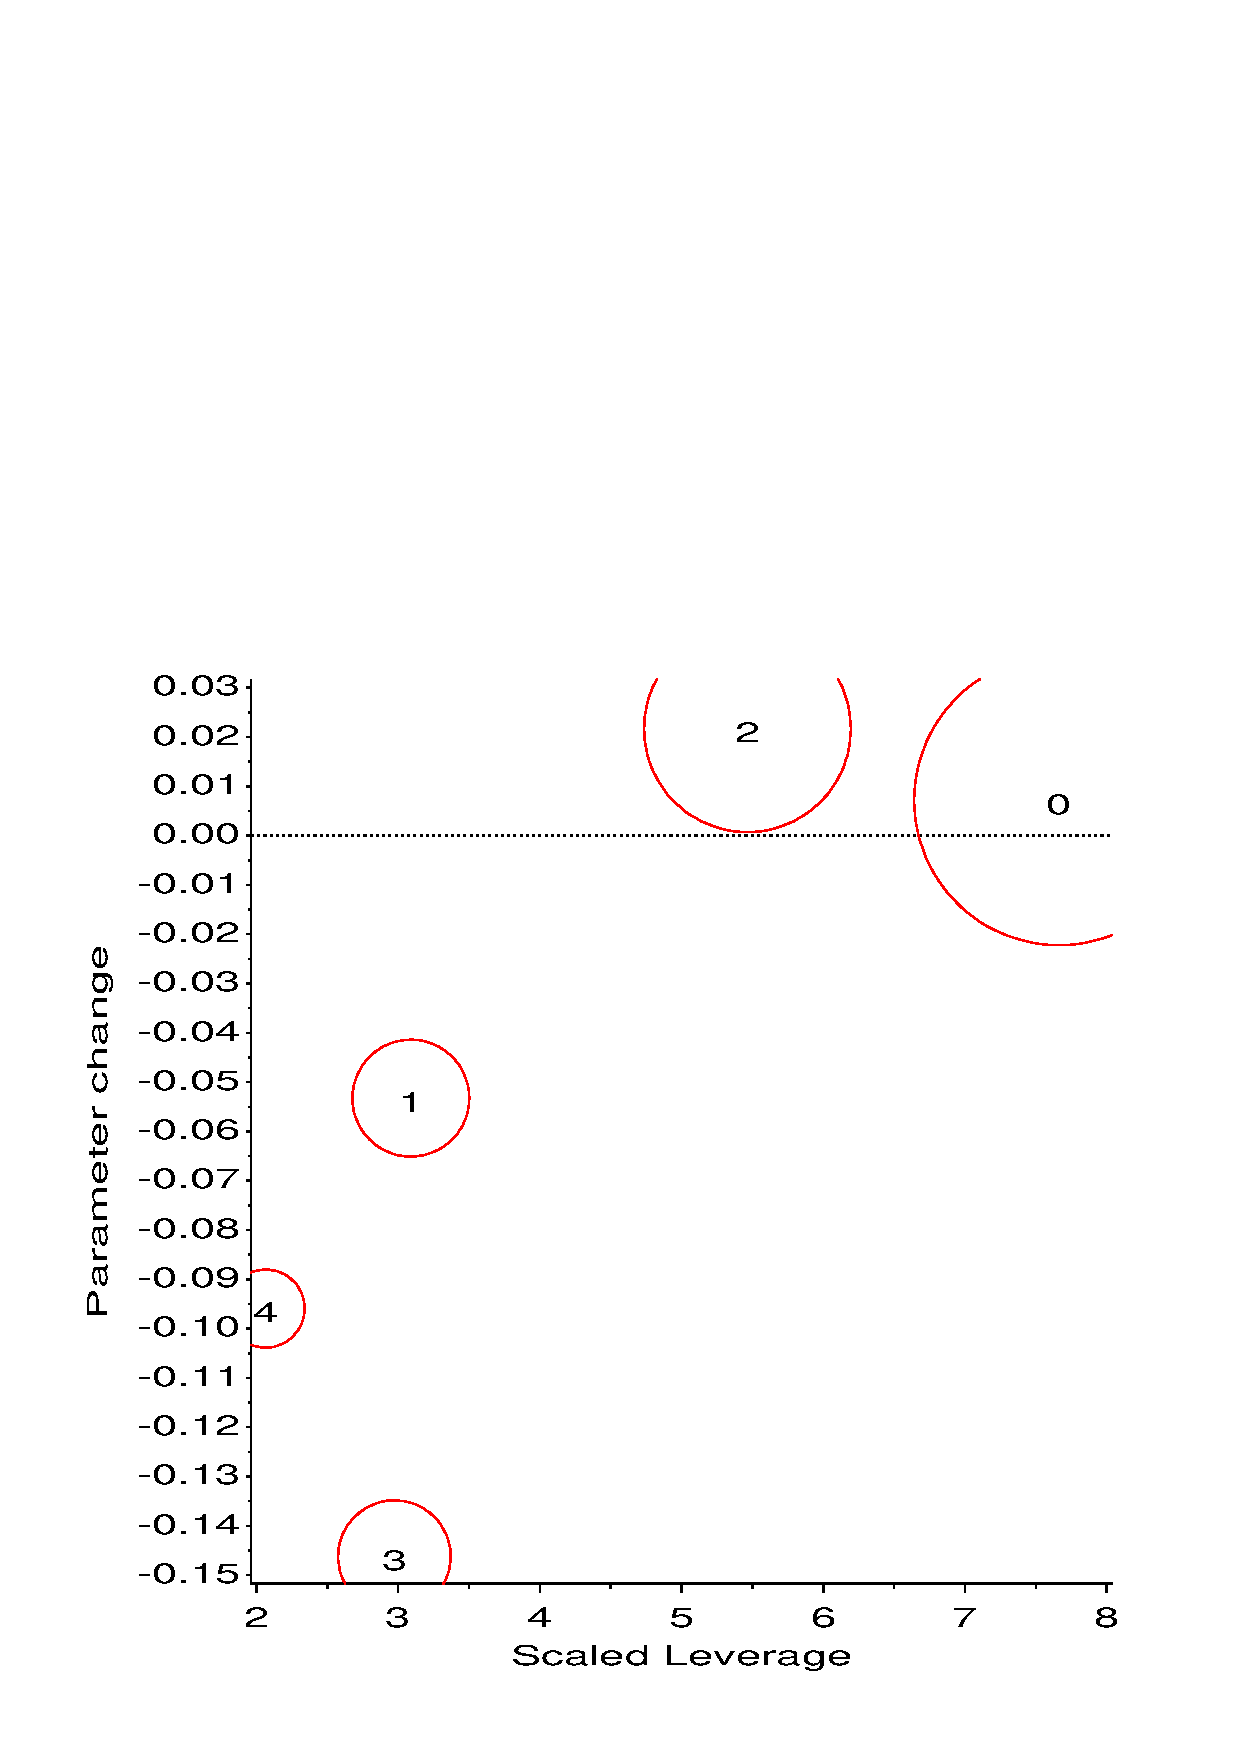
\includegraphics[scale=.5]{poisdemo4}\graphicsfile{ch2/fig/poisdemo4.eps}{}
  \caption[Influence plot for the Poisson parameter]{Influence plot
for the Poisson parameter, fitting the horse kick data.
  The ordinate shows the indicated change in $\lambda$
directly, and the bubble size is proportional to
influence.}\label{fig:poisdemo4} \end{figure}


\ix{Poissonness plot|)}

\subsection{Plots for other distributions}\label{sec:discrete-other}
As described in \secref{sec:pwrseries}, the binomial, Poisson, negative binomial,
geometric, and logseries distributions are all members of the
general  power series family of discrete distributions.
For this family, \citet{HoaglinTukey:85} develop similar plots
of a count metameter against $k$ which appear as a straight line
when a data distribution follows a given family member.

The distributions which can be analyzed in this way are shown in
\tabref{tab:distparms}, with the interpretation given to the
slope and intercept in each case.
For example, for the Binomial distribution, a ``binomialness''
plot is constructed by plotting $\log n_k^{*} / N \binom{n}{k}$
against $k$.  If the points in this plot approximate a straight
line, the slope is interpreted as $\log (p/(1-p))$, so the
binomial parameter $p$ may be estimated as $p = e^b/(1+e^b)$.
\begin{table}[htb]
\caption[Plot parameters for five discrete distributions]{Plot parameters for five discrete distributions. In each case the count metameter, $\phi
(n_k^{*})$ is plotted against $k$, yielding a straight line when the data
follow the given distribution.}
\label{tab:distparms}
 \begin{center}
\begin{tabular}{p{2.4cm}llll}
  \hline\\[.5ex]
  \tableheader
%              & Probability      & Count                      & Theoretical & Theoretical \\
%Distributiion & function, $p(k)$ & metameter, $\phi(n_k^{*})$ & Slope ($b$) & Intercept ($a$)\\[1ex]
  \multilineL{Distribution\\} & \multilineL{Probability\\function, $p(k)$} & \multilineL{Count)\\metameter, $\phi(n_k^{*})$} & \multilineL{Theoretical\\ slope ($b$)} &
  \multilineL{Theoretical\\ intercept ($a$)}
  \hline \\[.5ex]
Poisson          & $e^{-\lambda }\lambda ^k/k!$ & $\log (k!n_k^{*}/N)$ & $\log
(\lambda )$ & -$\lambda $ \\[.7ex]
%
Binomial          & $\binom nkp^k(1-p)^{n-k}$ & $\log \left( n_k^{*}/N\binom
nk\right) $ & $\log \left(\frac{p}{1-p}\right)$ & $n\log (1-p)$ \\[.7ex]
%
Negative binomial & $\binom{n+k-1}kp^n(1-p)^k$ & $\log \left( n_k^{*}/N%
\binom{n+k-1}k\right) $ & $\log (1-p)$ & $n\log (p)$ \\[.7ex]
%
Geometric         & $p(1-p)^k$ & $\log \left( n_k^{*}/N\right) $ & $\log (1-p)$ & $\log (p)$ \\[.7ex]
%
Log series        & $\theta ^k/[-k\log (1-\theta )]$ & $\log \left(
kn_k^{*}/N\right) $ & $\log (\theta )$ & $-\log \left( -\log (1-\theta)\right) $ \\[1ex]%
  \hline
  \multicolumn{5}{p{\textwidth}}{\emph{Source}: adapted from \citet{HoaglinTukey:85}, Table 9-15.} \\
\end{tabular}
 \end{center}
\end{table}



Unlike the Ord plot, a different plot is required for each distribution,
because the count metameter, \(\phi ( n_k )\), differs
from distribution to distribution.
Moreover, systematic deviation from a linear relationship does not
       indicate which distribution provides a better fit.
However, the attention to robustness, and the availability of confidence
intervals and influence diagnostics make this a highly useful tool
for visualizing discrete distributions.


\subsubsection{\macro{DISTPLOT}}
The \macro{DISTPLOT} (see \macref{mac:distplot}) carries out the analysis and produces overall
distribution plots and influence plots for the members of the
power series distributions shown in \tabref{tab:distparms}.
As with the \macro{GOODFIT} values for parameters for a given distribution
may be supplied
in the \mparm{PARM}{DISTPLOT}.

When the value of the distribution parameter
is not supplied, the macro produces the overall distribution plot
whose slope $b$ (and intercept $a$) are used to find graphical
estimates of the parameter.
For most distributions, the available MLE or moments estimates
given in \secref{sec:discrete-distrib}
are also calculated and displayed in the plot.
When the value of the distribution parameter is supplied,
a leveled plot is produced, with graphical parameter estimates adjusted
for the leveling.

\begin{Example}[saxony3]{Families in Saxony}
Our analysis in \exref{ex:saxony1} and \exref{ex:saxony2} of
the Saxony data
showed that the distribution of male children had slightly heavier tails
than the binomial.
We can see this even more clearly in the distribution diagnostic
plot produced
by the \macro{DISTPLOT}.  For a binomial distribution, we might call
this a ``binomialness plot''.

\figref{fig:saxony1} is produced with the statement
\begin{listing}
%distplot(data=saxony, count=males, freq=families, dist=binomial);
\end{listing}
The systematic curvature of the points again indicates the inadequacy
of the binomial, and the widths of the intervals around the points
show that the two extreme points are of limited reliability.
Comparing this plot with the hanging rootogram (\figref{fig:saxony}),
we see that heavy-tailed distributions will tend to curve upwards.
We also see that the estimate of $p = \exp(b) / [1+\exp(b)] $ from the slope of the fitted
line is quite close to the maximum likelihood estimate.
\begin{figure}[htb]
  \centering
  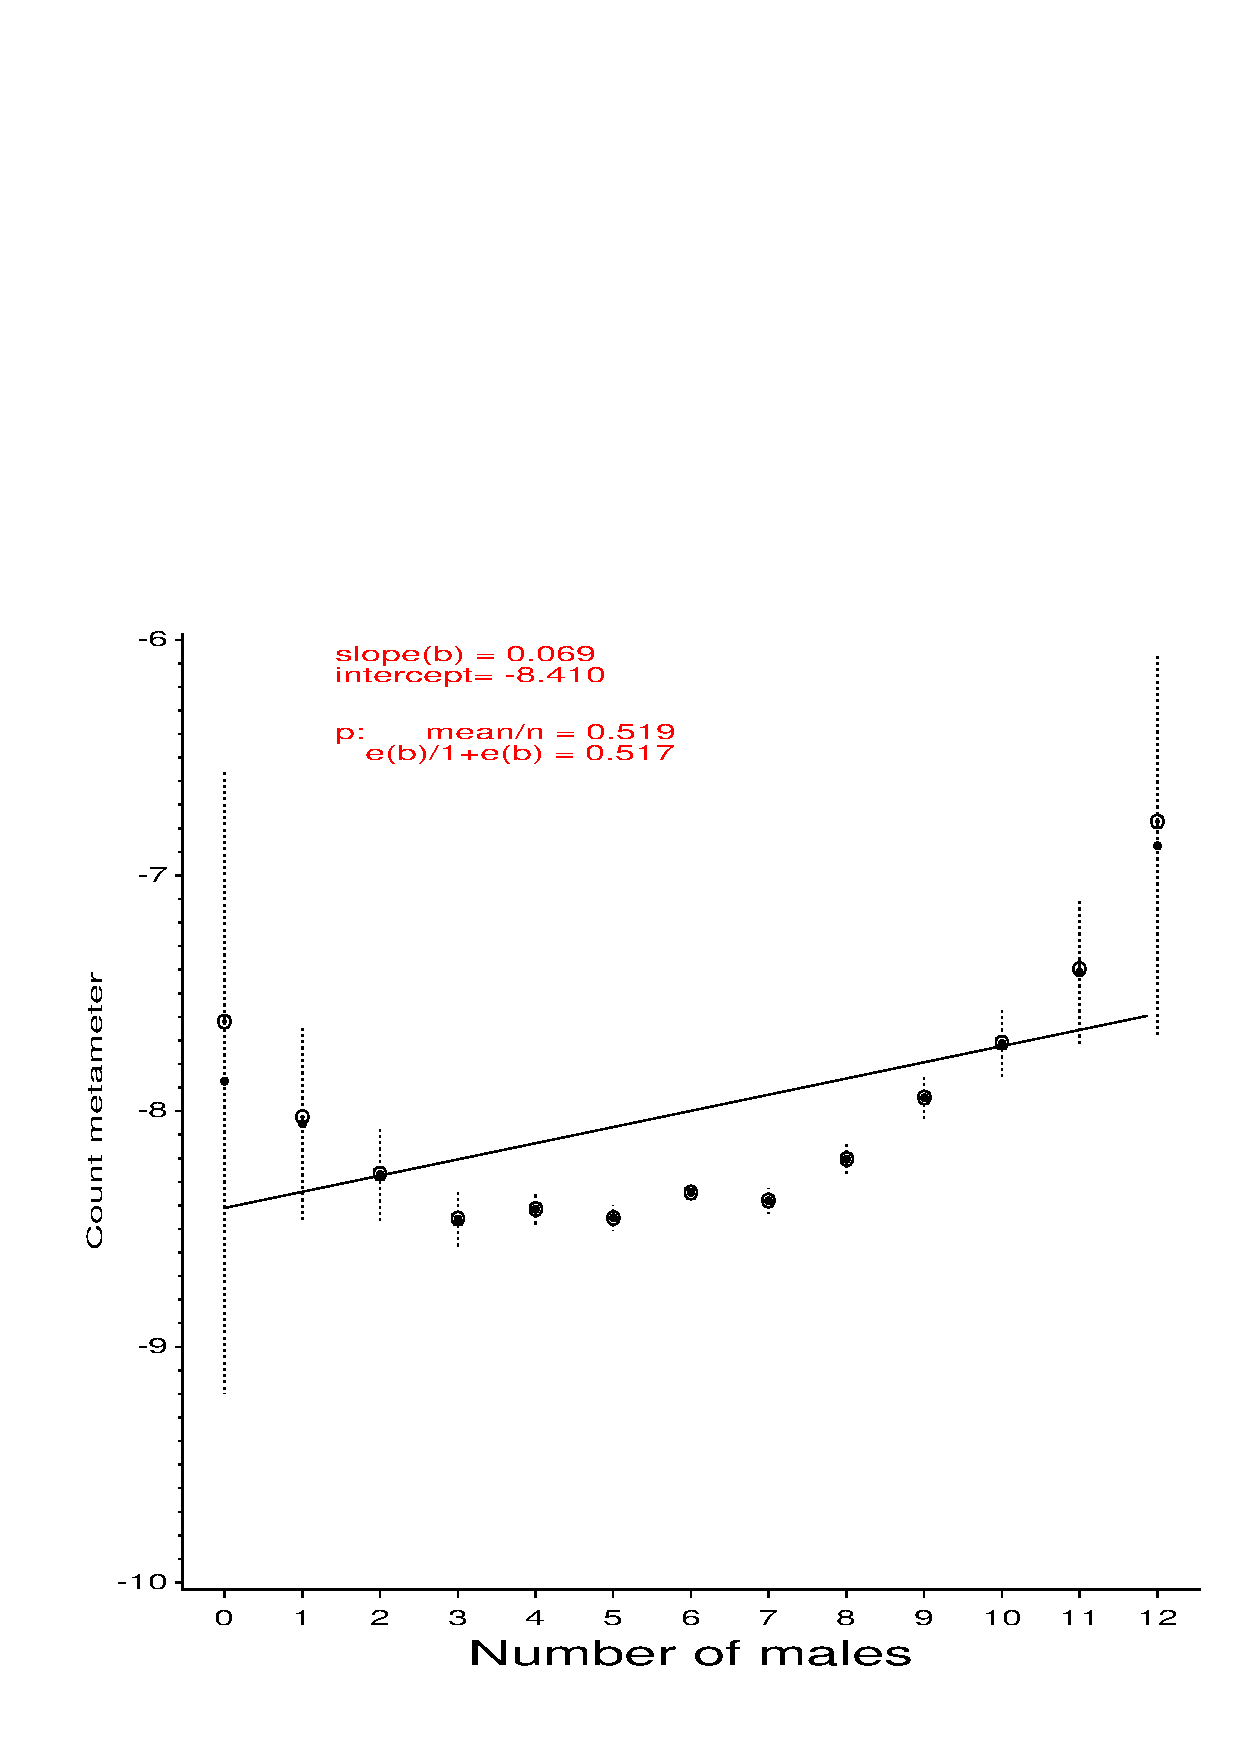
\includegraphics[scale=.6]{saxony1}\graphicsfile{ch2/fig/saxony1.eps}{}
  \caption{Binomialness plot for the distribution of males in Saxony families. }%
  \label{fig:saxony1}
\end{figure}
\end{Example}

%\section{Chapter summary}
\begin{itemize}
\item Correspondence analysis is an exploratory technique, designed to
show the row and column categories in a two- (or three-) dimensional
space.  These graphical displays, and various extensions, provide
ways to interpret the patterns of association and visually explore 
the adequacy of certain \loglin models.

\item The scores assigned to the categories of each variable are optimal
in several equivalent ways.
Among other properties,
they maximize the (canonical) correlations between the quantified
variables (weighted by cell frequencies), and make the regressions
of each variable on the other most nearly linear, for each CA dimension.

\item Multi-way tables may be analyzed in several ways.
In the ``stacking'' approach, two or more variables may be combined
interactively in the rows and/or columns of an \nway table.
Simple CA of the restructured table reveals associations between
the row and column categories of the restructured table,
but hides associations between the variables combined interactively.
Each way of stacking corresponds to a particular \loglin model
for the full table.

\item Multiple \ca is a generalization of CA to two or more variables
based on representing the data as an indicator matrix, or the Burt matrix.
The usual MCA provides an analysis of the joint, bivariate relations
between all pairs of variables.

% \item An extended form of MCA provides a means to display higher-order
% associations among multiple categorical variables.
% For $2^Q$ tables composed of $Q$ binary variables, this analysis yields
% simple geometric relations that may be interpreted in terms of odds ratios.
% \TODO{Delete this if \secref{sec:ca-mcainter} is not included.}

\item The biplot is a related technique for visualizing the elements of
a data array by points or vectors in a joint display of their row and
column categories. A standard CA biplot represents the contributions to
lack of independence as the projection of the points for rows
(or columns) on vectors for the other categories.

\item Another application of the biplot to \ctab data is described, based on analysis
of log frequency.
This analysis also serves to diagnose patterns of independence and
partial independence in two-way and larger tables.
\end{itemize}

%\section{Further reading}

\chapter{Two-way contingency tables}\label{ch:twoway}
\begin{center}
 \rule[-4pt]{0.5pt}{4pt}\hrulefill\rule[-4pt]{0.5pt}{4pt}\\
 \begin{minipage}[c]{.33\linewidth}
  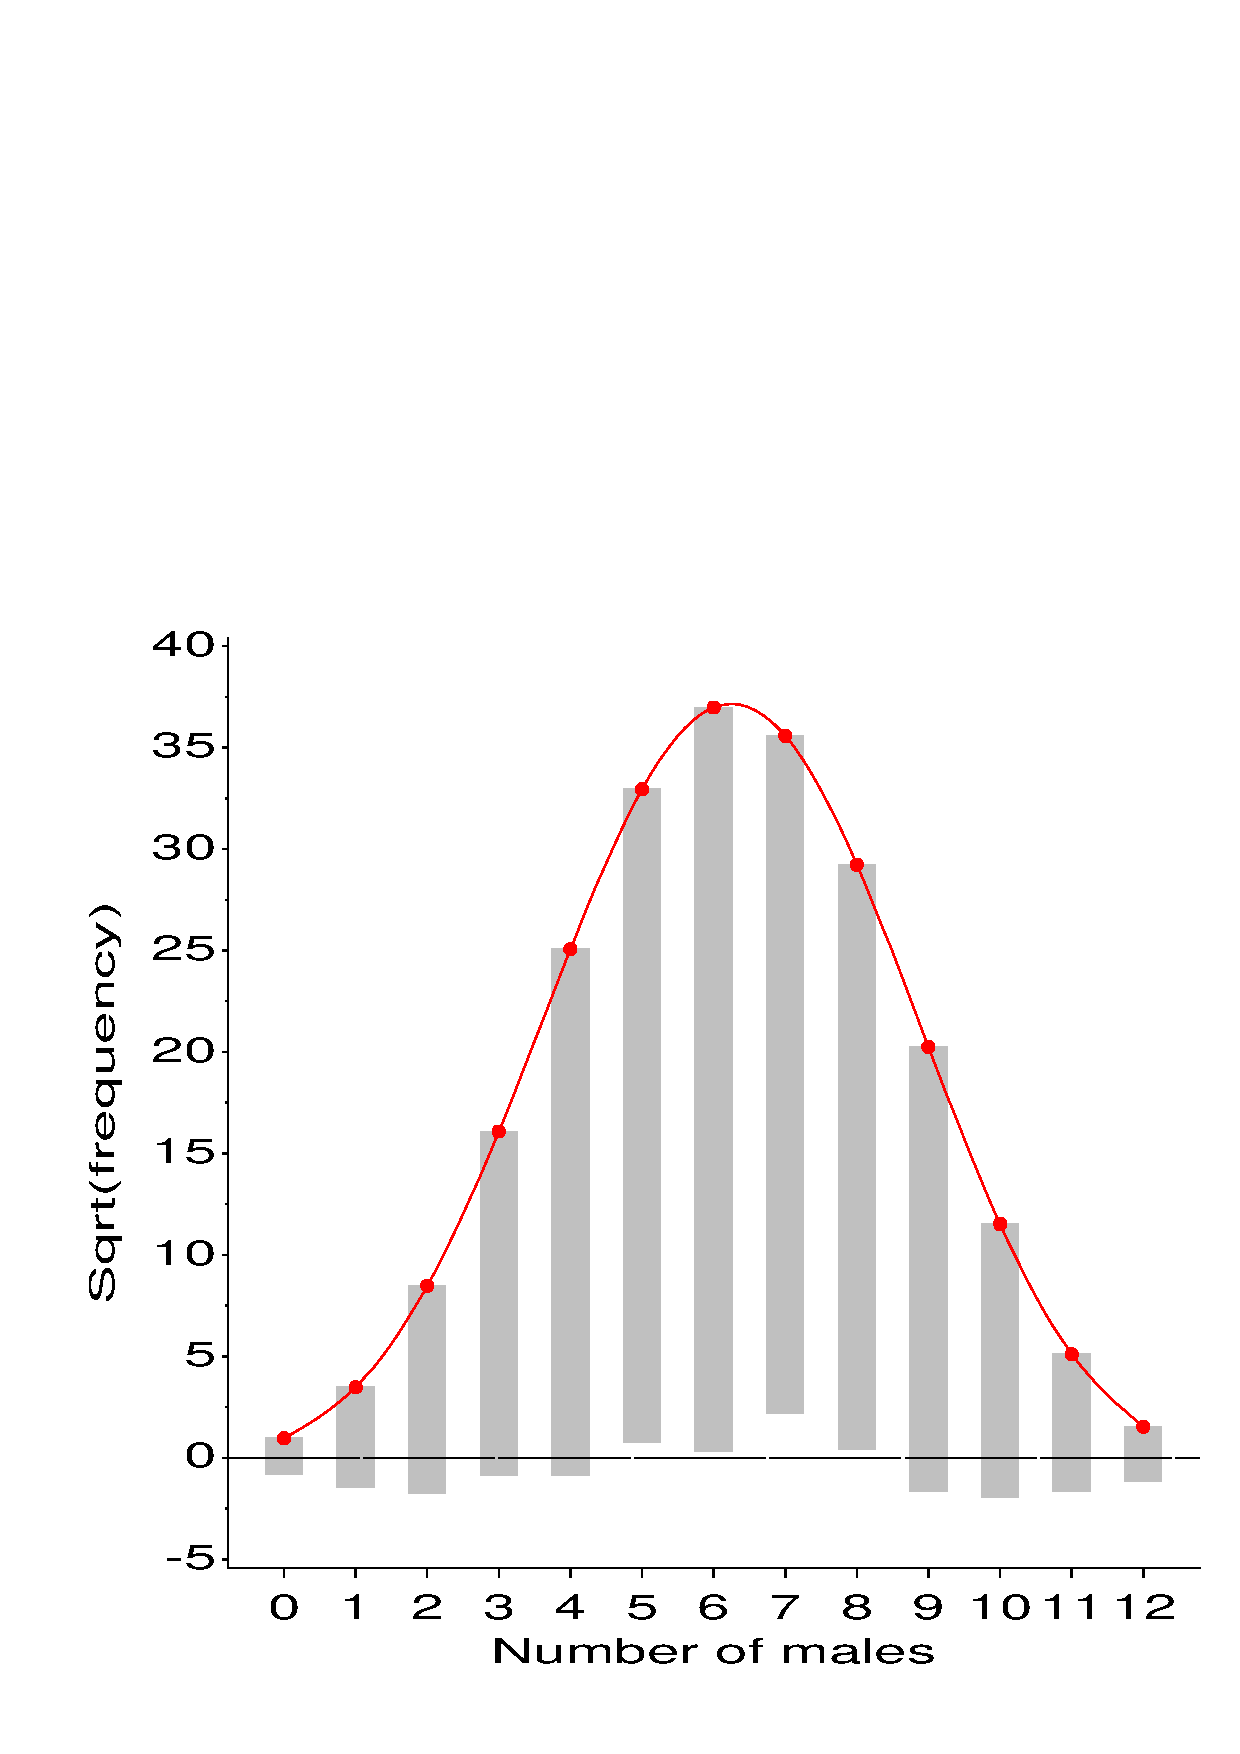
\includegraphics[width=1\linewidth]{saxony}\graphicsfile{ch2/fig/saxony.eps}{}
 \end{minipage}%
 \hfill
 \begin{minipage}[c]{.33\linewidth}
  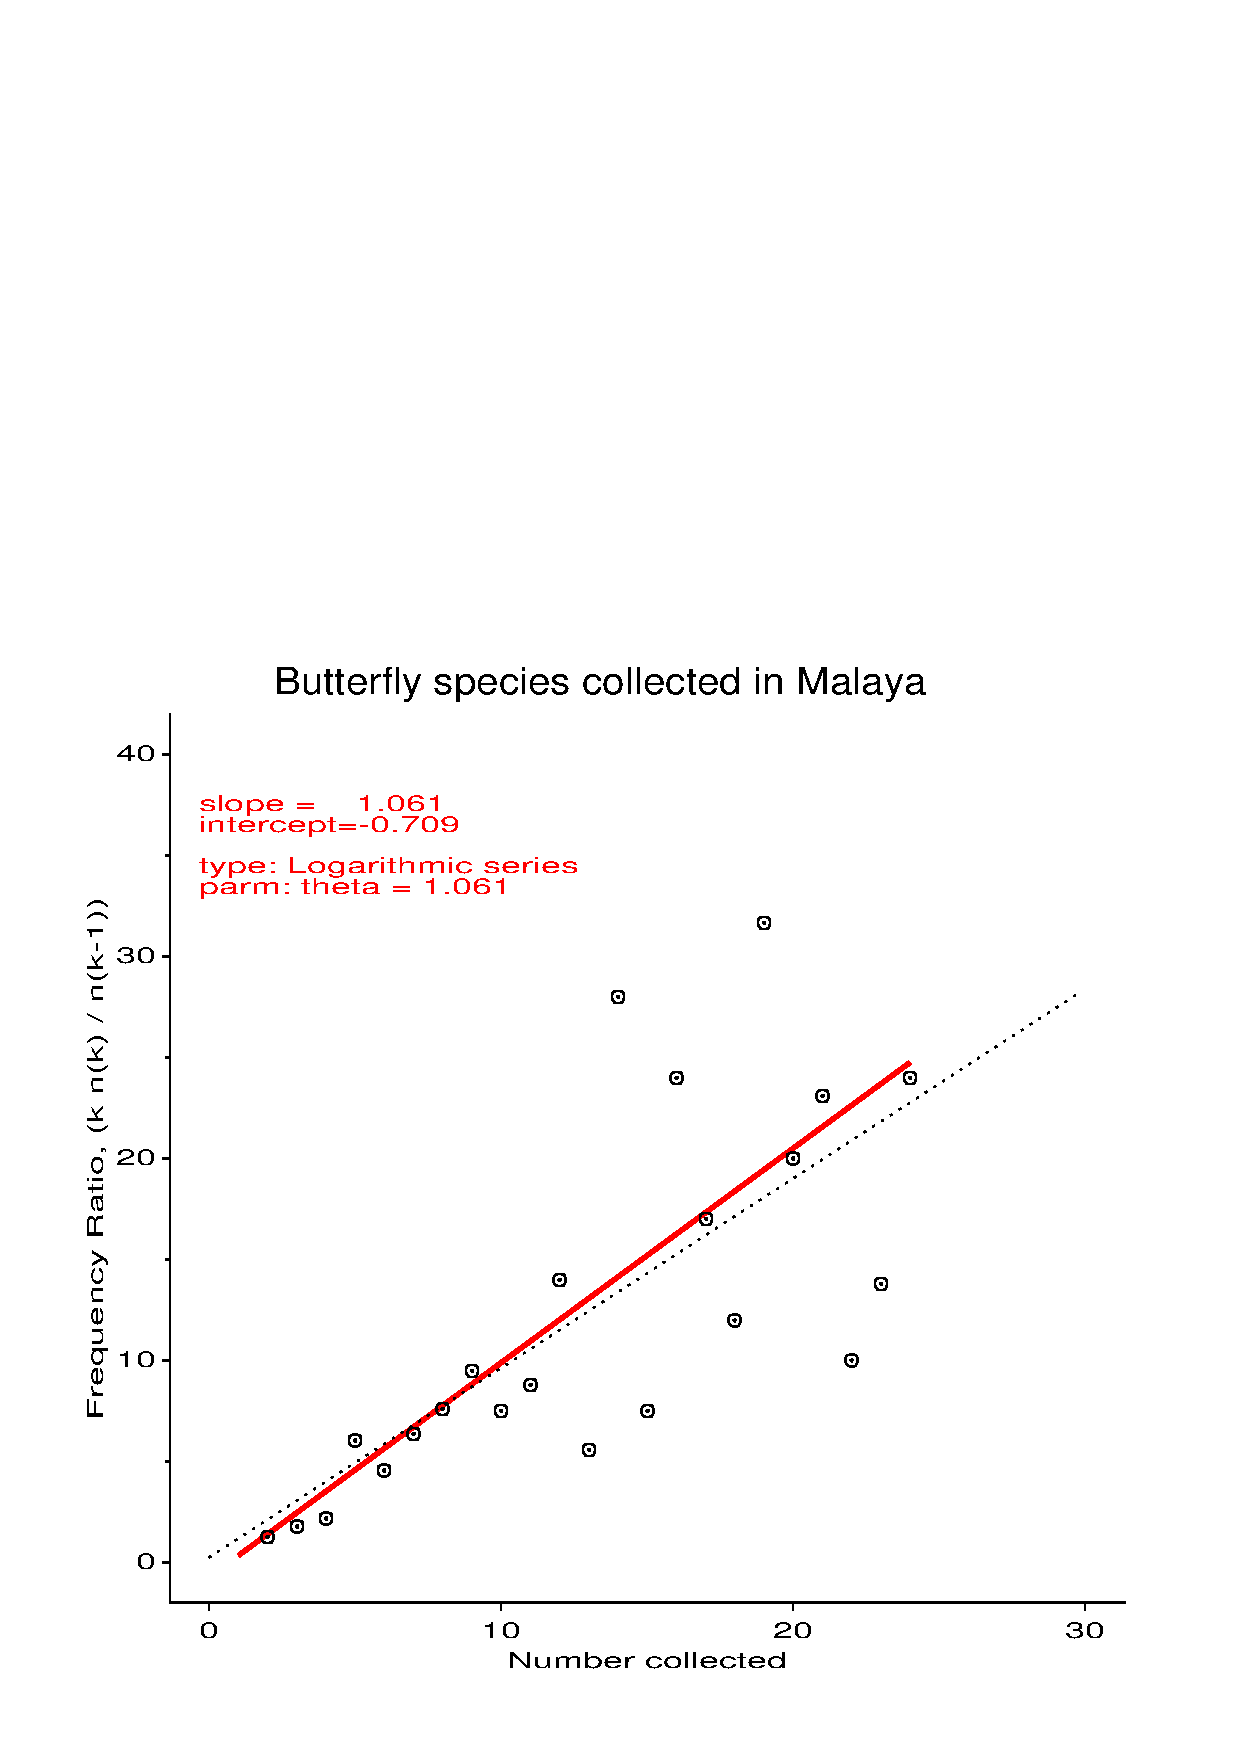
\includegraphics[width=1\linewidth]{orddemo3}\graphicsfile{ch2/fig/orddemo3.eps}{}
 \end{minipage}
 \hfill
 \begin{minipage}[c]{.33\linewidth}
  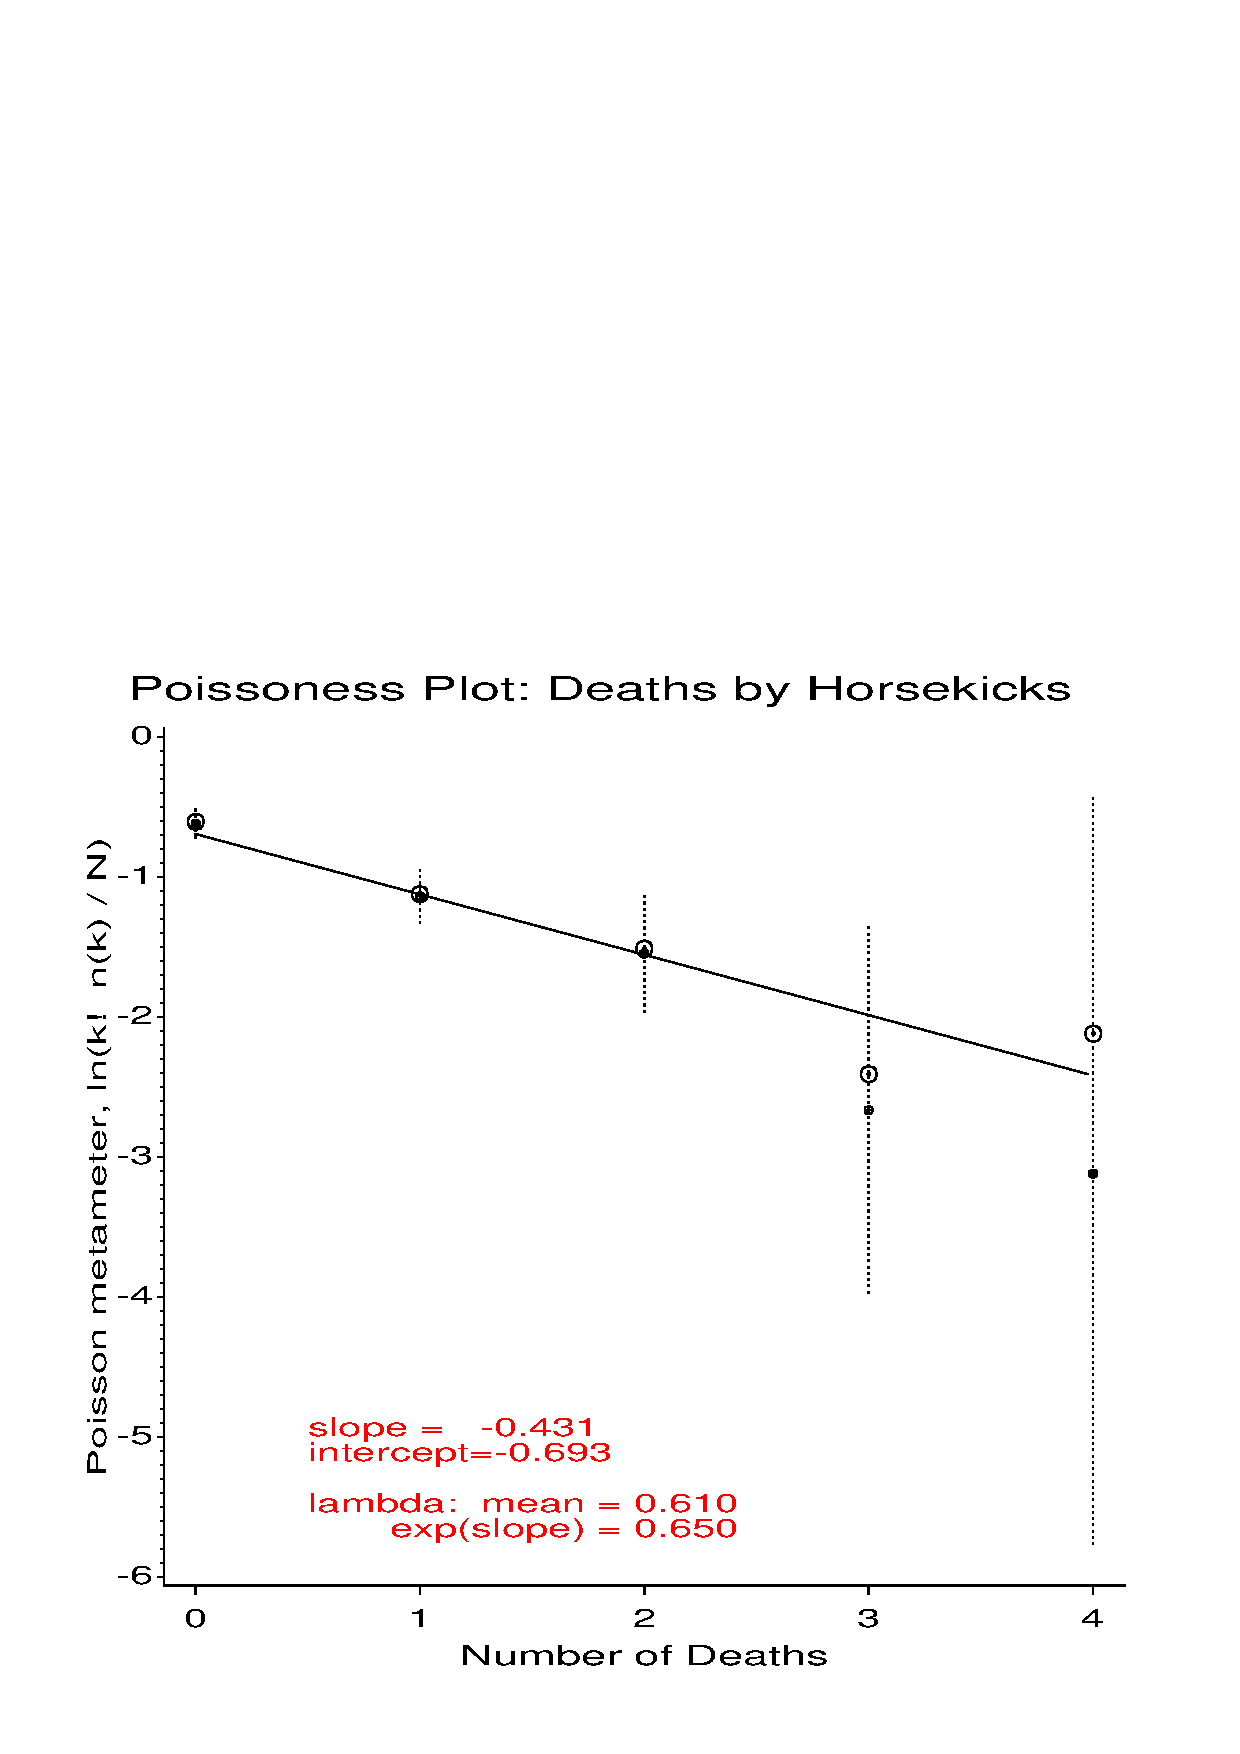
\includegraphics[width=1\linewidth]{poisdemo1}\graphicsfile{ch2/fig/poisdemo1.eps}{}
 \end{minipage}
\end{center}


\begin{quote}
{\Large\noindent
The analysis of two-way frequency tables concerns the association
between two variables.  Different specialized displays are focused
on visualizing an odds ratio ($2 \times 2$ tables), or the general
pattern of association, or the agreement between row and column
categories.}
\end{quote}
\minitoc
\clearpage

\section{Introduction}
\epigraph{If you choose to represent the various parts in life by
holes upon a table, of different shapes---some circular, some
triangular, some square, some oblong---we shall generally find that
the triangular person has got into the square hole, the oblong into
the triangular, and a square person has squeezed himself into the
round hole.}{Sydney Smith, 1769-1845}

Most methods of statistical analysis are concerned with understanding
relationships among variables.
With categorical variables, these relationships are usually
studied from data which has been
summarized by a
\glossterm{contingency table},
giving the frequencies of observations cross-classified
by two or more such variables.

This chapter is concerned with methods for understanding the association
between two categorical variables.
Some simple examples are also presented which involve a third, stratifying variable,
where we wish to determine if the relationship between two primary
variables is the same or different for all levels of the
stratifying variable.
Methods for fitting models and displaying associations for three-way
and larger tables are described in \chref{ch:mosaic}.

We describe briefly some methods for testing whether an association
exists between two variables and for quantifying the strength
of this association (\secref{sec:twoway-tests}).
In \secref{sec:twoway-strat} we extend these ideas to situations where
the relation between two variables is of primary interest, but there
are one or more background variables to be controlled.

The main emphasis, however, is on graphical methods which help
to describe the nature of an association between variables.
\secref{sec:twoway-fourfold} presents the fourfold display,
designed to portray the odds ratio in $2 \times 2$ tables or a set
of $k$ such tables.
Sieve diagrams (\secref{sec:twoway-sieve}) and association plots
(\secref{sec:twoway-assoc}) are more general methods for depicting
the pattern of associations an any two-way tables.
When the row and column variables represent the classifications
of different raters, specialized measures and visual displays
for inter-rater agreement (\secref{sec:twoway-agree}) are particularly
useful.
Another specialized display, the trilinear plot (\secref{sec:twoway-trilinear})
is designed
for three-column frequency tables or compositional data.
In order to make clear some of the distinctions which occur in
\ctab{} analysis, I begin with several examples.

\begin{Example}[berkeley1]{Berkeley admissions}
\tabref{tab:berk22} shows aggregate data on applicants to
graduate school at Berkeley for the six largest departments in 1973
classified by admission and gender
\citep{Bickel-etal:75}.
See \datref{dat:berkeley} for the complete data set.
For such data we might wish to study whether there is an association
between admission and gender.
Are male (or female) applicants more likely to be admitted?
The presence of an association might be considered as
evidence of sex bias in admission practices.

\tabref{tab:berk22} is an example of the simplest kind of \ctab,
a $2 \times 2$ classification of individuals according to two
dichotomous (binary) variables.
For such a table, the question of whether there is an association
between admission and gender is equivalent to asking if the
proportions of males and females who are admitted to graduate
school are the same, or whether the difference in proportions
admitted is zero.
\begin{table}[htb]
\caption{Admissions to Berkeley graduate programs}
\label{tab:berk22}
 \begin{center}
\begin{tabular}{lrr|rrr}
\hline
  & Admitted & Rejected & Total & \red{\% Admit} & \red{Odds(Admit)}\\
\hline
 Males & 1198 & 1493 & 2691  & \red{44.52} & \red{0.802}\\
 Females & 557 & 1278 & 1835 & \red{30.35} & \red{0.437}\\
\hline
 Total & 1755 & 2771 & 4526  & 38.78 & 0.633\\
\hline
\end{tabular}
\end{center}
\end{table}

\end{Example}

Although the methods for quantifying association in larger tables can be
used for $2 \times 2$ tables, there are specialized measures
(described in \secref{sec:twoway-tests}) and
graphical methods for these simpler tables.

It is frequently useful to make a distinction between \glossterm{outcome},
or response variables, on the one hand, and possible \glossterm{explanatory}
or predictor variables on the other.
In \tabref{tab:berk22}, it is natural to consider admission
as the outcome, and gender as the explanatory variable.
In other tables, no variable may be clearly identified as \emph{the}
outcome, or there may be several response variables.

\begin{Example}[haireye1]{Hair color and eye color}
\tabref{tab:hairdat} shows data collected by
\citet{Snee:74}
on the relation between hair color and eye color among 592
students in a statistics course
(\datref{dat:haireye}).  Neither hair color nor eye color
is considered a response in relation to the other;  our interest concerns
whether an association exists between them.
Hair color and eye color have both been classified
into four categories.  Although the categories used are among the most
common, they are not the only categories possible.%
\footnote{If students had been asked to write down their hair and eye
colors, it is likely that many more than four categories of each
would appear in a sample of nearly 600.}
Everyday observation suggests that there probably is an association
between hair color and eye color, and we will describe tests
and measures of associations for larger tables in
\secref{sec:twoway-overall}.
\begin{table}[htb]

\caption{Hair-color eye-color data}\label{tab:hairdat}
\begin{center}
\begin{tabular}{|lrrrr|r|}
\hline
        & \multicolumn{4}{c|}{Hair Color}        & \\
Eye     &         &         &         &         &       \\
Color   &  Black  &  Brown  &    Red  &  Blond  & Total \\[2ex] \hline
Green   &      5  &     29  &     14  &     16  &    64 \\
Hazel   &     15  &     54  &     14  &     10  &    93 \\
Blue    &     20  &     84  &     17  &     94  &   215 \\
Brown   &     68  &    119  &     26  &      7  &   220 \\[1ex] \hline
Total   &    108  &    286  &     71  &    127  &   592 \\ \hline
\end{tabular}
\end{center}
\end{table}


\end{Example}

Table variables may be treated simply as unordered,
\glossterm{nominal} variables,  or as
\glossterm{ordinal} variables, where the categories are
ordered according to some underlying dimension.
For example, the categories of hair color or eye color
are typically considered as nominal categories;
however, they
might arguably be considered to be ordered from light to dark.
When the variables are ordinal, more sensitive
and therefore more powerful tests of association can be used.

If, as we suspect, hair color and eye color are associated,
we would like to understand \emph{how} they are associated.
The graphical methods described later in this chapter help
reveal the pattern of associations present.

\begin{Example}[arthrit1]{Arthritis treatment}
The data in \tabref{tab:arthrit} compares an active treatment for rheumatoid
arthritis to a placebo
\citep{KochEdwards:88}.
The outcome reflects
whether individuals showed no improvement, some improvement, or
marked improvement.
Here, the outcome variable is an ordinal one, and it is probably
important to determine if the relation between treatment and outcome
is the same for males and females.
The data set is given more fully in \datref{dat:arthrit}.

This is, of course, a three-way table, with factors
Treatment, Sex, and Improvement.
If the relation between treatment and outcome is the same for
both genders, an analysis of the Treatment by Improvement
table (collapsed over sex) could be carried out.
Otherwise we could perform separate analyses for
men and women, or
treat the combinations of treatment and sex as four levels of
a ``population'' variable, giving a $4 \times 3$ two-way table.
These simplified approaches each ignore certain information
available in
an analysis of the full three-way table.
\begin{table}[tb]

\caption{Arthritis treatment data}\label{tab:arthrit}
\begin{center}
\begin{tabular}{ll|rrr|r}
\hline
     &  & \multicolumn{3}{c|}{Improvement}            &  \\
\hline
   Treatment&  Sex    &None    &Some    &Marked  &  Total \\[2ex]
\hline
   Active   &  Female &      6 &      5 &     16 &     27 \\
            &  Male   &      7 &      2 &      5 &     14 \\
\hline
   Placebo  &  Female &     19 &      7 &      6 &     32 \\
            &  Male   &     10 &      0 &      1 &     11 \\[1ex]
\hline
   Total    &         &     42 &     14 &     28 &     84 \\
\hline
\end{tabular}
\end{center}
\end{table}


\end{Example}

\section{Tests of association for two-way tables}\label{sec:twoway-tests}

\subsection{Notation and terminology}\label{sec:twoway-notation}
To establish notation, let \(\mat{N}  =  \{  n_{ij}  \}\) be the
observed frequency table of variables \(A\) and \(B\) with \(r\) rows
and \(c\) columns, as shown in \tabref{tab:rbyc}.
In what follows, a subscript is replaced by a ``$+$''
when summed over the corresponding variable, so \(n_{i+}  =  \sum_j \,
n_{ij}\) gives the total frequency in row \(i\), \(n_{+j}  =  \sum_i \,
n_{ij}\) gives the total frequency in column \(j\), and \(n_{++}  =
\sum_i \sum_j \,  n_{ij}\) is the grand total; for convenience,
\(n_{++}\) is also symbolized by \(n\).
\begin{table}[htb]
\caption[The R by C contingency table]{The $R \times C$ contingency table}
\label{tab:rbyc}
\vspace{1ex}
\begin{center}
\begin{tabular}{l|llll|l}
\hline
Row      & \multicolumn{4}{c|}{Column category}      &          \\
Category &   1      &   2      & $\cdots$  &  $C$    & Total    \\
\hline
   1     & $n_{11}$ & $n_{12}$ & $\cdots$ & $n_{1C}$ & $n_{1+}$ \\
   2     & $n_{21}$ & $n_{22}$ & $\cdots$ & $n_{2C}$ & $n_{2+}$ \\
$\vdots$ & $\vdots$ & $\vdots$ & $\cdots$ & $\vdots$ & $\vdots$ \\
   $R$   & $n_{R1}$ & $n_{R2}$ & $\cdots$ & $n_{RC}$ & $n_{R+}$   \\  
\hline
Total    & $n_{+1}$ & $n_{+2}$ & $\cdots$ & $n_{+C}$ & $n_{++}$   \\
\hline
\end{tabular}
\end{center}
\end{table}

When each observation is randomly sampled from some population
and classified on two categorical variables, $A$ and $B$,
we refer to the \glossterm{joint distribution} of these variables,
and let $\pi_{ij} = \Pr(A=i,\,B=j)$ denote the probability that
an observation is classified in row $i$, column $j$ (or cell $(ij)$)
in the table.
Corresponding to these population joint probabilities, the
cell proportions, $p_{ij} = n_{ij} / n$, give the sample joint
distribution.

The row totals $n_{i+}$ and column totals $n_{+j}$ are called marginal frequencies for variables $A$ and $B$ respectively.
These describe the distribution of each variable \emph{ignoring} the other.
For the population probabilities, the \glossterm{marginal distributions}
are defined analogously as the row and column totals of the 
joint probabilities,
$\pi_{i+} = \sum_j \pi_{ij}$, and
$\pi_{+j} = \sum_i \pi_{ij}$.
The sample marginal proportions are, correspondingly, 
$p_{i+} = \sum_j p_{ij} = n_{i+} / n$, and 
$p_{+j} = \sum_i p_{ij} = n_{+j} / n$.

When one variable (the column variable, $B$, for example) is a response
variable, and the other ($A$) is an explanatory variable,
it is most often useful to examine the distribution of the response $B$
for \emph{each} level of $A$ separately.
These define the \glossterm{conditional distributions} of $B$, given the
level of $A$, and are defined for the population as
$\pi_{j\given i} = \pi_{ij} / \pi_{i+}$.

These definitions are illustrated in \outref{out:berkfreq.1}.
For the Berkeley data (\tabref{tab:berk22}), it shows the joint frequencies, $n_{ij}$, and joint sample percentages,
$100 \times p_{ij}$, in the first two rows within each table cell.
The third row in each cell (``Row pct'')
gives the conditional percentage of admission or rejection,
$100 \times p_{j\given i}$ for males and females separately.
The row and column labelled ``Total'' give the
marginal frequencies, $n_{i+}$ and $n_{+j}$,
and marginal percentages, $p_{i+}$ and $p_{+j}$.

\begin{Output}[htb]
\caption{Admission to Berkeley graduate programs: joint, marginal, and conditional percents}\label{out:berkfreq.1}
\small
\verbatiminput{ch\thechapter/out/berkfreq.1}
\end{Output}

\renewcommand{\FileName}{twobytwo}

\begin{frame}
%\makeatletter\slidebox@restore\makeatother
\frametitle{Graphical Methods for 2$\times$2 tables: Example}
\begin{itemize}
 \item \citet{Bickel-etal:75}: data on admissions to graduate departments
 at Berkeley in 1973.
 \item Aggregate data for the six largest departments:
 \begin{table}[htb]
\caption{Admissions to Berkeley graduate programs}
\label{tab:berk22}
 \begin{center}
\begin{tabular}{lrr|rrr}
\hline
  & Admitted & Rejected & Total & \red{\% Admit} & \red{Odds(Admit)}\\
\hline
 Males & 1198 & 1493 & 2691  & \red{44.52} & \red{0.802}\\
 Females & 557 & 1278 & 1835 & \red{30.35} & \red{0.437}\\
\hline
 Total & 1755 & 2771 & 4526  & 38.78 & 0.633\\
\hline
\end{tabular}
\end{center}
\end{table}


 \item Evidence for gender bias?
 \begin{itemize}

 \item Odds ratio, 
 $\theta = \frac{\mbox{Odds}(\mbox{Admit}\given\mbox{Male})}{\mbox{Odds}(\mbox{Admit}\given\mbox{Female})} = 
 \frac{1198 / 1493}{557 / 1276} = \frac{0.802}{0.437} = 
 1.84$
 \item $\rightarrow$ Males 84\% more likely to be admitted. 
 \item Chi-square tests: $G^2_{(1)} = 93.7$, $\chi^2_{(1)} = 92.2, \: p < 0.0001$
 \end{itemize}
\end{itemize}

\end{frame}
\begin{frame}[plain]
\begin{center}
\includegraphics[width=.7\textwidth]{fig/Admissions2}
\end{center}
\begin{itemize*}
 \item How to analyse these data?
 \item How to visualize \& interpret the results?
 \item Does it matter that we collapsed over Department?
\end{itemize*}


\end{frame}

\subsection{Standard analysis}
\begin{frame}[fragile]
% \makeatletter\slidebox@restore\makeatother
 \frametitle{Standard analysis: PROC FREQ}

% \vspace{2ex}
\begin{Input}
 proc freq data=berkeley;
   weight freq;
   tables gender*admit / chisq;
\end{Input}
 Output:
\begin{Output}[gobble=7,baselinestretch=.8]
               Statistics for Table of gender by admit

       Statistic                     DF       Value      Prob
       ------------------------------------------------------
       Chi-Square                     1     92.2053    <.0001
       Likelihood Ratio Chi-Square    1     93.4494    <.0001
       Continuity Adj. Chi-Square     1     91.6096    <.0001
       Mantel-Haenszel Chi-Square     1     92.1849    <.0001
       Phi Coefficient                       0.1427          
\end{Output}
 How to visualize and interpret?
\end{frame}

\subsection{Fourfold displays}
\begin{frame}
% \makeatletter\slidebox@restore\makeatother
 \frametitle{Fourfold displays for 2 $\times$ 2 tables}
 \begin{itemize*}
 \item \boldital{Quarter circles}: radius $\sim \sqrt{n_{ij}} \Rightarrow$
 \textbf{area} $\sim$ \textbf{frequency}
 \item \boldital{Independence}: Adjoining quadrants $\approx$ align
 \item \boldital{Odds ratio}: ratio of areas of diagonally opposite cells
 \item \boldital{Confidence rings}: Visual test of 
 $H_0 : \theta = 1 \leftrightarrow$ \alert{adjoining rings overlap}

 \begin{center}
   \includegraphics[width=.45\dispwidth,clip]{fig/pie2x2g}
 \end{center}
 \item Confidence rings do not overlap: $\theta \neq 1$  (reject $H_0$)
 \end{itemize*}
\end{frame}

\begin{frame}
 %\makeatletter\slidebox@restore\makeatother
 \frametitle{Fourfold displays for 2 $\times$ 2 $\times $ \textit{k} tables}
 \begin{itemize*}
 \item Data in \tabref{tab:berk22} had been pooled over departments
 \item Stratified analysis: one fourfold display for each department
 \item Each $2 \times 2$ table standardized to equate marginal frequencies
 \item Shading: highlight departments for which $H_a : \theta_i \ne 1$

 \begin{center}
 %  \includegraphics[width=.6\dispwidth,clip]{fig/pie2x2bb.eps}
   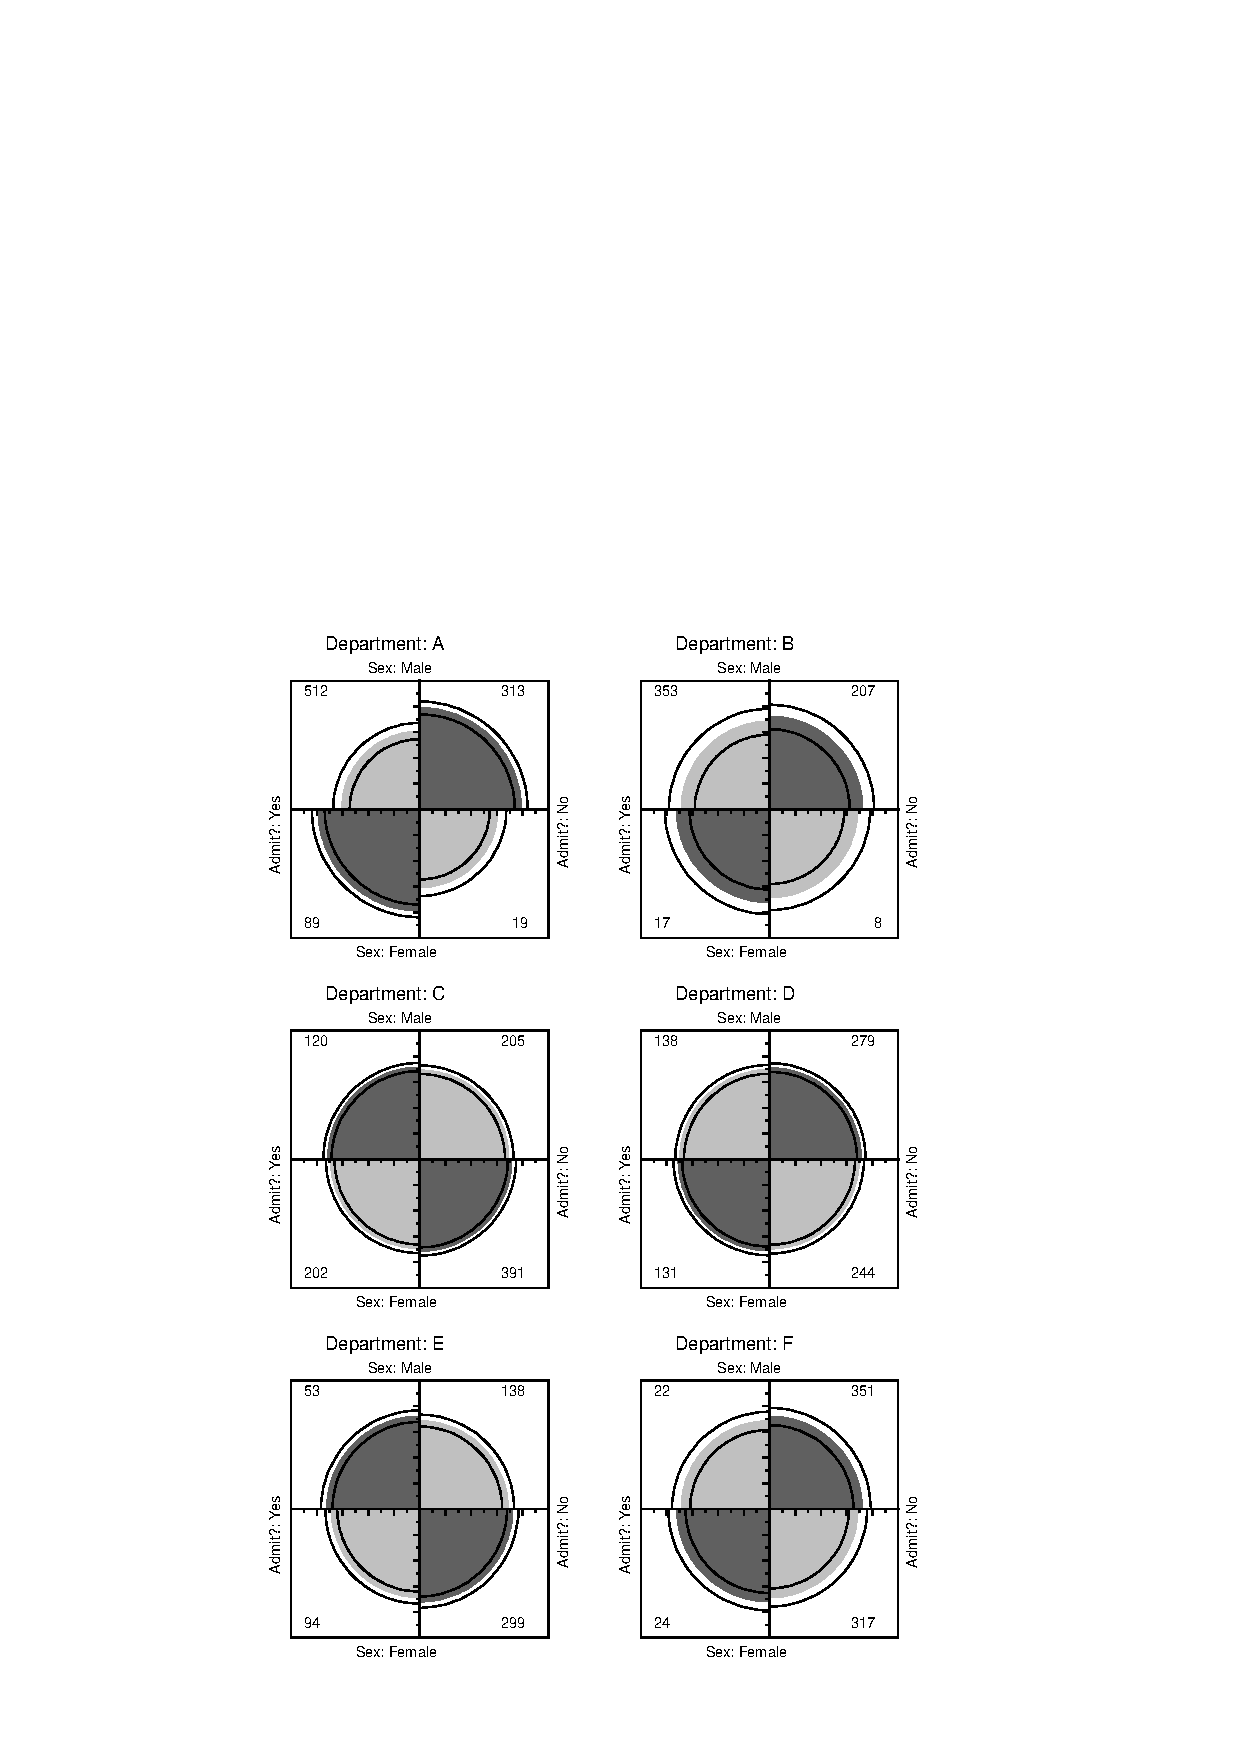
\includegraphics[width=.6\dispwidth,clip]{fig/pie2x2b}
 \end{center}
 \item Only one department (A) shows association; $\theta_A = 0.349 \rightarrow
 $ women $(0.349)^{-1} = 2.86$ times as likely as men to be admitted.
 \end{itemize*}
 \end{frame}

\begin{frame}
 %\makeatletter\slidebox@restore\makeatother
   \frametitle{What happened here?}
  Why do the results \emph{collapsed over} department disagree with the results \emph{by} department?
  \begin{block}{Simpson's paradox}
   \begin{itemize}
	 \item<1-> Aggregate data are misleading because they falsely
	 assume men and women apply \emph{equally} in each field.
	 \item<2-> But:
	   \begin{itemize*}
	   \item Large differences in admission rates across departments.
	   \item Men and women apply to these departments differentially.
	   \item Women applied in large numbers to departments with low admission rates.
	 \end{itemize*}
	 \item<3->
	  Other graphical methods can show these effects.
 	 \item<3-> (This ignores possibility of \emph{structural bias} against women:
	 differential funding of fields to which women are more likely to apply.)
  \end{itemize}
  \end{block}
\end{frame}

\begin{frame}[fragile]
%\makeatletter\slidebox@restore\makeatother

\frametitle{The \sasprogt{FOURFOLD} and the \macrot{FFOLD}}
  \begin{itemize*}
  \item The \sasprog{FOURFOLD} is written in \IML.
  \item The \macro{FFOLD} provides a simpler interface.
  \item Printed output: (a) significance tests for individual odds ratios,
  (b) tests of homogeneity of association (here, over departments) and
  (c) conditional association (controlling for department).
  \end{itemize*}
Plot by department:
\begin{Input}[fontsize=\small,label=\fbox{\texttt{berk4f.sas}},baselinestretch=0.8]
%include catdata(berkeley);

%ffold(data=berkeley, 
   var=Admit Gender,       \sascomment{/* panel variables   */} 
   \sasemph{by=Dept},                \sascomment{/* stratify by dept  */}
   down=2, across=3,       \sascomment{/* panel arrangement */}
   htext=2);               \sascomment{/* font size         */}
\end{Input}
Aggregate data: first sum over departments,
using the \macro{TABLE}:
\begin{Input}[fontsize=\small,baselinestretch=0.9,firstnumber=8]
%table(data=berkeley, \sasemph{out=berk2}, 
   var=Admit Gender,       \sascomment{/* omit dept          */}
   weight=count,           \sascomment{/* frequency variable */}
   order=data);
%ffold(\sasemph{data=berk2}, var=Admit Gender);
\end{Input}
\end{frame}

\subsection{Odds ratio plots}
\begin{frame}[fragile]
\frametitle{Odds ratio plots}
\begin{Rin}
> library(vcd)
> oddsratio(UCBAdmissions, log=FALSE)
\end{Rin}
\begin{Rout}
    A     B     C     D     E     F 
0.349 0.803 1.133 0.921 1.222 0.828 
\end{Rout}
\begin{Rin}
> lor <- oddsratio(UCBAdmissions)  # capture log odds ratios
> plot(lor)
\end{Rin}
\begin{center}
   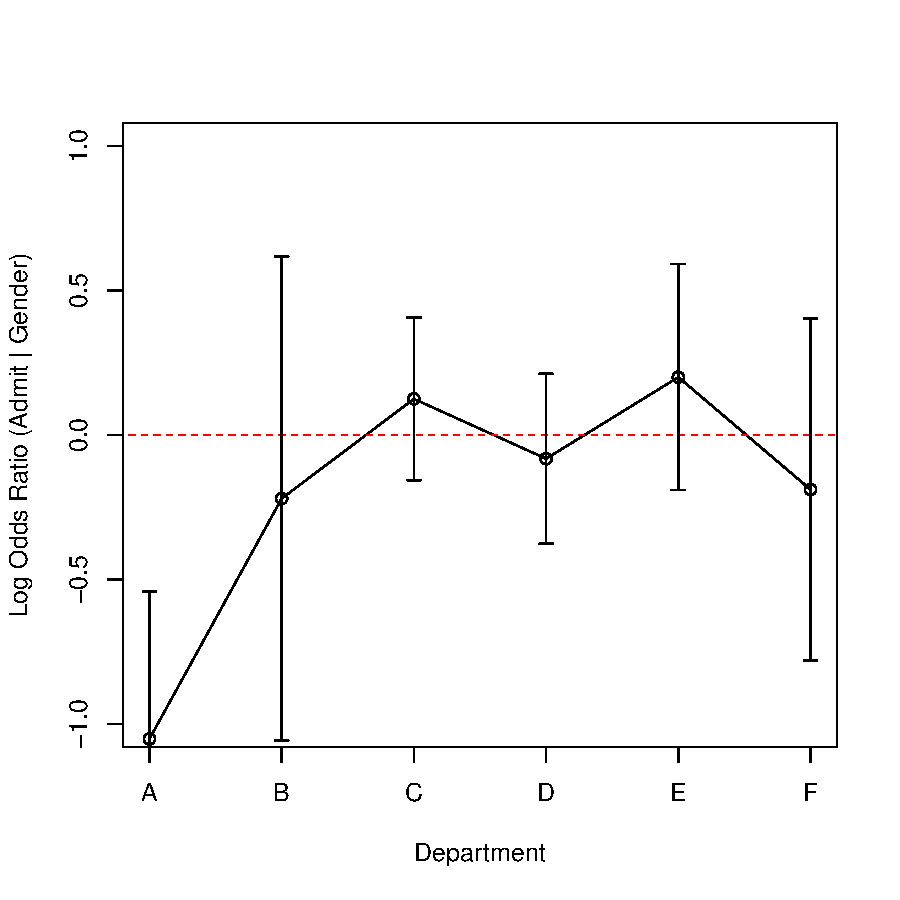
\includegraphics[width=.45\dispwidth,clip,trim=0 20 20 40]{fig/vcd-tut-oddsratio}
\end{center}

\end{frame}


\subsection{Larger tables---Overall analysis}\label{sec:twoway-overall}
For two-way tables overall tests of association can be carried out
using \PROC{FREQ}.
If the table has more than two factors (as in the
Arthritis Treatment data), the other factors will be
ignored (and collapsed) if not included the
\texttt{TABLES} statement.
This simplified analysis may be misleading if
the excluded factors interact with the factors used in the
analysis.

\begin{Example}[arthrit2]{Arthritis treatment}
Since the main interest is in the relation between treatment and
outcome, an overall analysis (which ignores sex) could be carried out
using \PROC{FREQ} as shown below.
\ixd{arthritis treatment}

\begin{listing}
title 'Arthritis Treatment: PROC FREQ Analysis';
data arth;
   input sex$ treat$ @;
   do improve = 'None  ', 'Some', 'Marked';
      input count @;
      output;
      end;
datalines;
Female  Active    6  5  16
Female  Placebo  19  7   6
Male    Active    7  2   5
Male    Placebo  10  0   1
;
*-- Ignoring sex;
proc freq order=data;
   weight count;
   tables treat * improve / cmh chisq nocol nopercent;
   run;
\end{listing}

In this analysis, note that:
\begin{itemize}
\item TREAT and IMPROVE are both character variables, which \PROC{FREQ}
       orders alphabetically (i.e., `Marked', `None', `Some') by
       default.  Because I want to treat the IMPROVE variable as
       ordinal, I used \texttt{order=data} on the \PROC{FREQ}
       statement to have the levels of IMPROVE ordered by their order
       of appearance in the \Dset.

\ix{Cochran-Mantel-Haenszel tests|(}
\item The \opt{chisq}{FREQ} gives the usual \(\chi^2\) tests
       (Pearson, Fisher's, etc.).  The \opt{cmh}{FREQ} requests the
       \IX{Cochran-Mantel-Haenszel tests}, including specialized
		 tests for ordinal variables.
\end{itemize}
The output, shown in \outref{out:arthfreq.1}, begins with the frequency table, including row
percentages.  The row percentages show a clear effect of treatment:
for people given the Active treatment, 51\% showed Marked improvement,
while among those given the Placebo, 67\% showed no improvement.

The results for the \opt{chisq}{FREQ} are also shown in \outref{out:arthfreq.1}.  All tests
show a significant association between treatment and outcome.

\begin{Output}
\caption{Arthritis treatment data, overall analysis}\label{out:arthfreq.1}
\small
\verbatiminput{ch3/out/arthfreq.1}
\end{Output}
\end{Example}

\subsection{Tests for ordinal variables}\label{sec:ordinaltests}

For \(r \times  c\) tables, different tests are applicable depending
on whether either or both of the row and column variables are
ordinal.  Tests which take the ordinal nature of a variable into
account are provided by the \opt{cmh}{FREQ} on the
\stmt{tables}{FREQ}.
These tests are based on assigning numerical scores to
the table categories;  the default (table) scores treat the levels as
equally spaced.  They generally have higher power when the pattern of
association is determined by the order of an ordinal variable.

For the arthritis data, these tests (\opt{cmh}{FREQ}) give the
output shown in \outref{out:arthfreq.2}.

\begin{Output}
\caption{Arthritis treatment data, overall analysis}\label{out:arthfreq.2}
\small
\verbatiminput{ch3/out/arthfreq.2}
\end{Output}

The three types of tests differ in the types of departure from
independence they are sensitive to:

\begin{itemize}
\item \boldital{General Association}.  When the row and column
       variables are both nominal (unordered) the only alternative
       hypothesis of interest is that there is \emph{some} association
       between the row and column variables.  The CMH test statistic
       is similar to the (Pearson) Chi-Square and Likelihood Ratio
       Chi-Square in the Statistics table; all have \((r - 1) (c -
       1)\) df.
\ix{Cochran-Mantel-Haenszel tests!general association}
\ix{likelihood ratio test}

\item \boldital{Row Mean Scores Differ}.  If the column variable is
       ordinal, assigning scores to the column variable produces a
       mean for each row.  The association between row and column
       variables can be expressed as a test of whether these means
       differ over the rows of the table, with \(r - 1\) df.  This
       is analogous to the Kruskal-Wallis non-parametric test (ANOVA
       based on rank scores).
\ix{Kruskal-Wallis test}
\ix{Cochran-Mantel-Haenszel tests!row means differ}

\item \boldital{Nonzero Correlation (Linear association)}.  When {\bf both} row and
       column variables are ordinal, we could assign scores to both
       variables and compute the correlation ($r$).  The Mantel-Haenszel
       \(\chi^2\) is equal to \(( N - 1) r^2\), where N is the total
       sample size.  The test is most sensitive to a pattern where
       the row mean score changes linearly over the rows.
\end{itemize}
\ix{Cochran-Mantel-Haenszel tests!linear association}
{\bf Notes}:

\begin{itemize}
\item Different kinds of scores can be assigned using the
\opt{scores}{FREQ}
on the \stmt{tables}{FREQ}, but only the
relative spacing of the scores is important.
The default, \pname{SCORES=TABLE} uses integer row and column numbers
for character variables, and numeric levels (or formatted equivalents)
for numeric variables.

\item When only one variable is ordinal, make it the {\bf last} one
       on the \stmt{tables}{FREQ}, because \PROC{FREQ} only computes
       means across the column variable.
\item When there are only $r=2$ rows (as there are here), the 
nonzero correlation and row
       means tests are equivalent.
		 In a $2 \times 2$ table, all three tests are identical.
\end{itemize}

\subsection{Sample CMH Profiles}\label{sec:Sample}

Two contrived examples may make the differences among these tests
more apparent.  Visualizations of the patterns of association
reinforces the aspects to which the tests are most sensitive.

\subsubsection{General Association}
\ix{Cochran-Mantel-Haenszel tests!general association|(}
The table below exhibits a
general association between variables $A$ and $B$, but no difference in
row means or linear association.  The row means are calculated by
assigning integer scores, $b_i = i$ to the column categories.
\figref{fig:cmhdemo}(a) shows
the pattern of association in this table graphically, as a sieve diagram
(described in \secref{sec:twoway-sieve}).

 \begin{center}
 \begin{tabular}{r|rrrrr|rr}
  \hline
   & b1 & b2 & b3 & b4 & b5 & Total & Mean \\ 
  \hline
  a1 & 0 & 15 & 25 & 15 & 0 & 55 & 3.0 \\ 
  a2 & 5 & 20 & 5 & 20 & 5 & 55 & 3.0 \\ 
  a3 & 20 & 5 & 5 & 5 & 20 & 55 & 3.0 \\ 
  \hline
  Total & 25 & 40 & 35 & 40 & 25 & 165 & 3.0\\ 
  Mean & 2.8 & 1.6 & 1.4 & 1.6 & 2.8 & 2.1\\
  \hline
 \end{tabular}
 \end{center}


This is reflected in the \PROC{FREQ} output shown in
\outref{out:cmhdemo.1}.
The chi-square values for non-zero correlation and different
row mean scores are exactly zero because the row means are all equal.
Only the general association test shows that $A$ and $B$
are associated.
\begin{Output}[ht]
\caption{General Association example: CMH tests}\label{out:cmhdemo.1}
\small
\verbatiminput{ch3/out/cmhdemo.1}
\end{Output}
\ix{Cochran-Mantel-Haenszel tests!general association|)}

\subsubsection{Linear Association}
\ix{Cochran-Mantel-Haenszel tests!linear association|(}
The table below contains a weak,
non-significant general association, but significant row mean
differences and linear associations.
The unstructured test of general association would therefore
lead to the conclusion that no association exists, while the
tests taking ordinal factors into account would conclude otherwise.
Note that the largest frequencies
shift towards lower levels of $B$ as the level of variable $A$ increases.
See \figref{fig:cmhdemo}(b) for a visual representation of this pattern.

 \begin{center}
 \begin{tabular}{r|rrrrr|rr}
  \hline
     & b1 & b2 & b3 & b4 & b5 & Total & Mean \\ 
  \hline
  a1 & 2 & 5 & 8 & 8 & 8 & 31 & 3.48 \\ 
  a2 & 2 & 8 & 8 & 8 & 5 & 31 & 3.19 \\ 
  a3 & 5 & 8 & 8 & 8 & 2 & 31 & 2.81 \\ 
  a4 & 8 & 8 & 8 & 5 & 2 & 31 & 2.52 \\ 
  \hline
  Total & 17 & 29 & 32 & 29 & 17 & 124 & 3.00 \\ 
  Mean & 3.1 & 2.7 & 2.5 & 2.3 & 1.9 & 2.5\\
  \hline
 \end{tabular}
 \end{center}


Note that the \(\chi^2\)-values for the row-means and non-zero
correlation tests in \outref{out:cmhdemo.2}
are very similar, but the correlation test is more
highly significant since it is based on just one degree of
freedom.

\begin{Output}[htb]
\caption{Linear Association example: CMH tests}\label{out:cmhdemo.2}
\small
\verbatiminput{ch3/out/cmhdemo.2}
\end{Output}

The differences in sensitivity and power among these tests is
analogous to the difference between general ANOVA tests and tests for
linear trend in experimental designs with quantitative factors:
The more specific test has greater power, but is sensitive to
a narrower range of departure from the null hypothesis.


%% two subfig side-by-side
\begin{figure}[htb]
 \begin{minipage}[b]{.49\linewidth}
  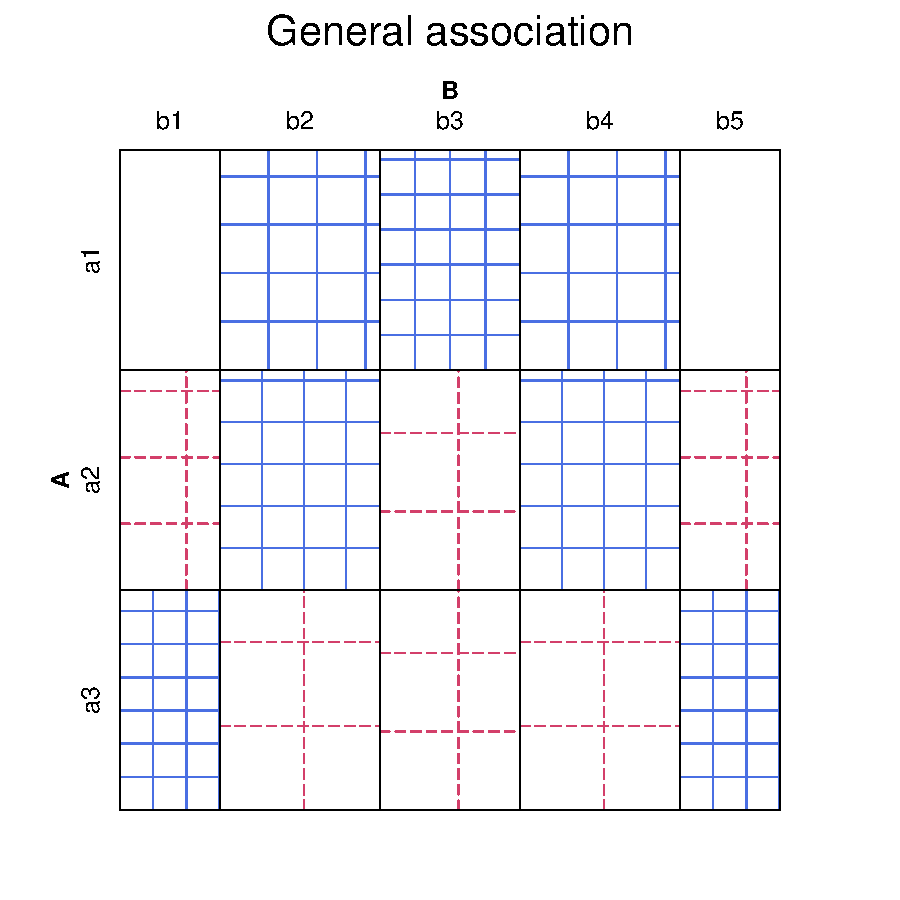
\includegraphics[width=1\linewidth]{ch3/fig/cmhdemo1}
 \end{minipage}%
 \hfill
 \begin{minipage}[b]{.49\linewidth}
  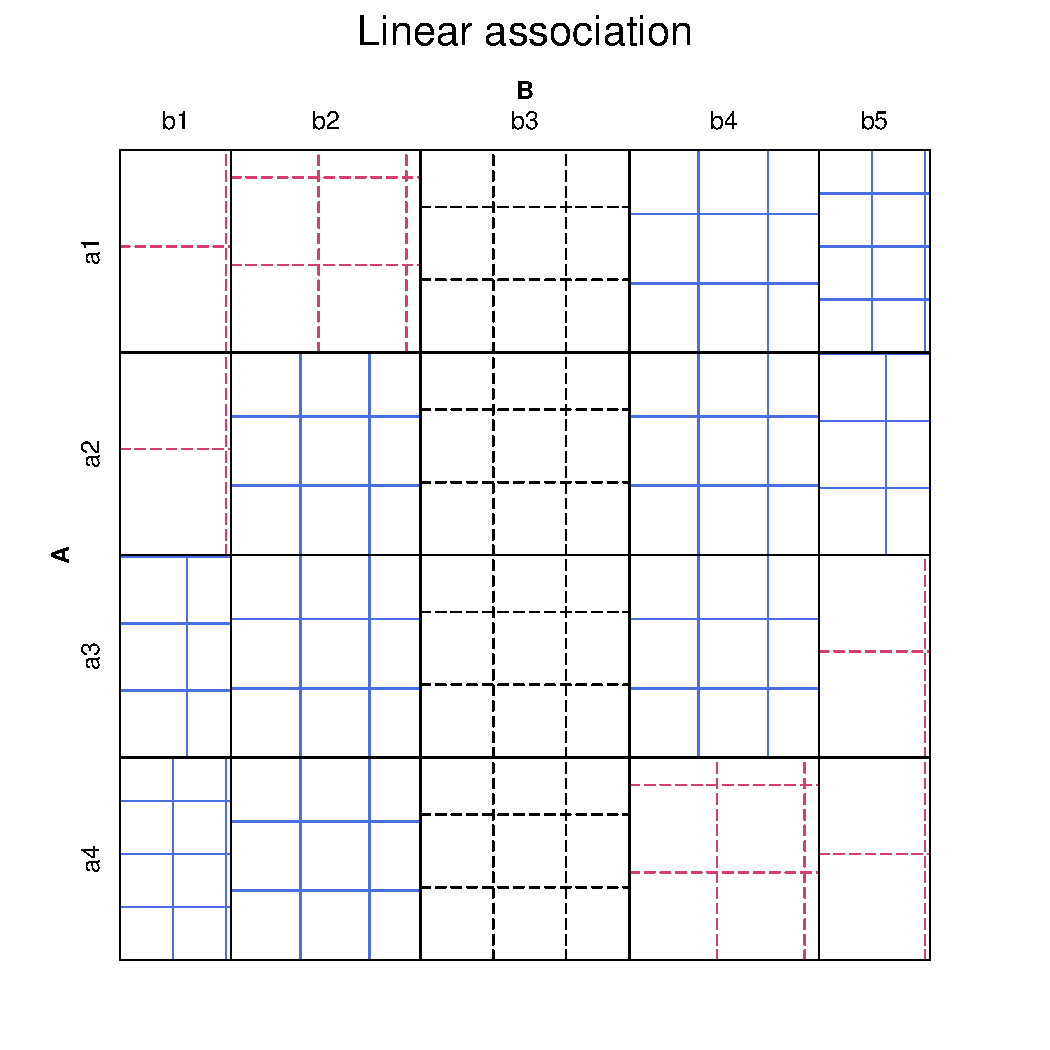
\includegraphics[width=1\linewidth]{ch3/fig/cmhdemo2}
 \end{minipage}
 \caption[Sieve diagrams for general association and linear association]{Sieve diagrams for two patterns of association. (a) General association (b) linear association.
 In each figure,
 cells with greater than expected frequency are shown with solid, blue cross hatching and the number of boxes is proportional to the observed frequency.}\label{fig:cmhdemo}
\end{figure}
\ix{Cochran-Mantel-Haenszel tests!linear association|)}
\ix{Cochran-Mantel-Haenszel tests|)}

\section{Stratified analysis}\label{sec:twoway-strat}
An overall analysis ignores other variables (like sex), by
collapsing over them.  It is possible that the treatment is effective
only for one gender, or even that the treatment has opposite effects
for men and women.
\ixd{arthritis treatment}

A stratified analysis:

\begin{itemize}

\item controls for the effects of one or more background variables.
       This is similar to the use of a blocking variable in an ANOVA
       design.

\item is obtained by including more than two variables in the {\tt
       tables} statement.  List the stratification variables {\bf
       first}.  To examine the association between TREAT and IMPROVE,
       controlling for both SEX and AGE (if available):

\begin{equation*}
   \mbox{\texttt{tables }}
   \overbrace{\rule{0in}{1.5ex}\mbox{\texttt{ age * sex }}}^{\mbox{\scriptsize stratify by}}
   \mbox{\texttt{ * }}
   \overbrace{\rule{0in}{1.5ex}\mbox{\texttt{ treat }}}^{\mbox{\scriptsize explanatory}}
   \mbox{\texttt{ * }}
   \overbrace{\rule{0in}{1.5ex}\mbox{\texttt{ improve;}}}^{\mbox{\scriptsize response}}
\end{equation*}

\end{itemize}

\begin{Example}[arthrit3]{Arthritis treatment}
The statements below request a stratified analysis of the arthritis
treatment data
with CMH tests,
controlling for sex.

{\small
\begin{verbatim}
*-- Stratified analysis, controlling for sex;
proc freq order=data;
   weight count;
   tables sex * treat * improve / cmh chisq nocol nopercent;
   run;
\end{verbatim}
}

\PROC{FREQ} gives a separate table for each level of the stratification
variables (\outref{out:arthfreq.3} and \outref{out:arthfreq.4}), plus overall (partial) tests controlling for the
stratification variables (\outref{out:arthfreq.5}).
\ixd{arthritis treatment}

\begin{Output}[htb]
\caption{Arthritis treatment data, stratified analysis}\label{out:arthfreq.3}
\small
\verbatiminput{ch3/out/arthfreq.3}
\end{Output}

Note that the strength of
association%
\glosstex{meas of assoc}
between treatment and outcome is quite
strong for females (\outref{out:arthfreq.3}).  In contrast, the results for males (\outref{out:arthfreq.4}) shows
a not-quite significant association, even by the 
more powerful Mantel-Haenszel test.
However,
note that there are too few males for the general association
\(\chi^2\) tests to be reliable (the statistic does not follow the
theoretical \(\chi^2\) distribution).
\begin{Output}[htb]
\caption{Arthritis treatment data, stratified analysis}\label{out:arthfreq.4}
\small
\verbatiminput{ch3/out/arthfreq.4}
\end{Output}

The individual tables are followed by the (overall) partial tests of
association controlling for sex, shown in \outref{out:arthfreq.5}.  Unlike the tests for each stratum,
these tests {\bf do not} require large sample size in the individual
strata -- just a large total sample size.  Note that the \(\chi^2\)
values here are slightly larger than those from the initial analysis
that ignored sex.
\ixd{arthritis treatment}

\begin{Output}[htb]
\caption{Arthritis treatment data, stratified analysis}\label{out:arthfreq.5}
\small
\verbatiminput{ch3/out/arthfreq.5}
\end{Output}
\end{Example}

\subsection{Assessing homogeneity of association}
In a stratified analysis
it is often of interest to know if the association between the
primary table variables is the same over all strata.  For \(k \times
2 \times  2\) tables this question reduces to whether the \IX{odds ratio} is
the same in all k strata, and \PROC{FREQ} computes the \IX{Breslow-Day test}
for homogeneity of odds ratios
when you use the \opt{measures}{FREQ} on the {\tt
tables} statement.  \PROC{FREQ} cannot perform tests of homogeneity for
larger tables, but these can be easily done with the \texttt{CATMOD}
procedure.
\ix{homogeneity of association}

\begin{Example}[arthrit4]{Arthritis treatment}
For the arthritis data, homogeneity means that there is no three-way
Sex * Treatment * Outcome association.  That is, the association
between treatment and outcome (\texttt{improve})
is the same for both men and women.
This hypothesis can be stated
as the \loglin\ model,
\begin{equation}\label{eq:STO2}
 \textrm{[SexTreat] [SexOutcome] [TreatOutcome]}
 \period
\end{equation}
This notation (described in \secref{sec:loglin-counts})
lists only the high-order association
terms in a linear model for log frequency.
Thus, the model \eqref{eq:STO2}
allows associations between sex and treatment (e.g., more males
get the Active treatment), between sex and outcome (e.g. females
are more likely to show marked improvement),
and between treatment and outcome,
but no three-way association.
In the \PROC{CATMOD} step
below, the \stmt{LOGLIN}{CATMOD} specifies this \loglin\  model
as \pname{sex|treat|improve@2} (where \texttt{improve} is the Outcome variable)
which means ``all terms up to 2-way
associations''.

\begin{listing}
title2 'Test homogeneity of treat*improve association';
data arth;
   set arth;
   if count=0 then count=1E-20;
proc catmod order=data;
   weight count;
   model sex * treat * improve = _response_ /
         ml noiter noresponse nodesign nogls ;
   loglin sex|treat|improve@2 / title='No 3-way association';
run;
   loglin sex treat|improve   / title='No Sex Associations';
\end{listing}
\ixd{arthritis treatment}

(Frequencies of zero can be regarded as either ``structural
zeros''---a cell which could not occur, or as ``sampling zeros''---a
cell which simply did not occur.  \PROC{CATMOD} treats zero frequencies
as ``structural zeros'', which means that cells with \texttt{count = 0}
are excluded from the analysis.  The DATA step above replaces the one
zero frequency by a small number.)
\ix{structural zeros}
\ix{sampling zeros}
\ix{zeros!structural}
\ix{zeros!sampling}

In the output from \PROC{CATMOD}
shown in \outref{out:arthfreq.7}, the likelihood ratio \(\chi^2\) (the
badness-of-fit for the No 3-Way model) is the test for homogeneity
across sex.  This is clearly non-significant, so the
treatment-outcome association can be considered to be the same for
men and women.

\begin{Output}[htb]
\caption{Arthritis treatment data, testing homogeneity}\label{out:arthfreq.7}
\small
\verbatiminput{ch3/out/arthfreq.7}
\end{Output}

Note that the associations of sex with treatment and sex with outcome
are both small and of borderline significance, which suggests a
stronger form of homogeneity, the log-linear model [Sex]
[TreatOutcome] which says the only association is that between
treatment and outcome.  This model is tested by the second {\tt
loglin} statement given above, which produced the results shown
in \outref{out:arthfreq.8}.
The likelihood ratio test indicates that this model might provide a
reasonable fit.
\ix{homogeneity of association}
\begin{Output}[htb]
\caption{Arthritis treatment data, testing homogeneity}\label{out:arthfreq.8}
\small
\verbatiminput{ch3/out/arthfreq.8}
\end{Output}
\end{Example}


\section{Fourfold display for 2 x 2 tables}\label{sec:twoway-fourfold}
\ixon{fourfold display}
The \boldital{fourfold display} is a relative of the pie chart,
designed for the display of $2 \times 2$ (or $2 \times 2 \times k$)
tables
\citep{Fienberg:75,Friendly:94b,Friendly:94c}.
In this display the frequency
\(n_{ij}\) in each cell of a fourfold table is shown by a quarter
circle, whose radius is proportional to \(\sqrt { n_{ij} }\), so the
area is proportional to the cell count.
The fourfold display
is similar to a pie chart in using segments of
a circle to show frequencies.  It
differs from a pie chart in that it keeps the
angles of the segments constant and varies the radius,
whereas the pie chart varies the angles and keeps the radius constant.

The main purpose of this display is to depict the sample odds ratio,
\(\hat{\theta} = (n_{11} /  n_{12} )
\div  (n_{21} /  n_{22} )\).  An association between the variables
(\(\theta \neq 1\)) is shown by the tendency of diagonally opposite
cells in one direction to differ in size from those in the opposite
direction, and the display uses color or shading to show this
direction.  Confidence rings for the observed \(\theta\) allow a
visual test of the hypothesis of independence,
 \(H_0 :  \theta  =  1\).  They have
the property that (in a standardized display) the rings for adjacent quadrants overlap \emph{iff}
the observed counts are consistent with the null hypothesis.

\begin{Example}[berkeley2]{Berkeley admissions}
\figref{fig:fourfold11} shows the basic fourfold display for the
Berkeley admissions data (\tabref{tab:berk22}).
Here, the area of each quadrant is proportional to the cell frequency,
shown numerically in each corner.
The odds ratio is proportional to the product of the areas
shaded dark, divided by the product of the areas shaded light.
The sample odds ratio, Odds (Admit\(|\)Male) / Odds(Admit\(|\)Female) is
1.84 (see \exref{ex:berkeley1a})
indicating that males were nearly twice as likely to be admitted.

However, it is difficult to make these visual comparisons
because there are more men than women, and because the
proportions admitted and rejected are unequal.  In the unstandardized
display the confidence bands have no interpretation as a test
of \(H_0 :  \theta  =  1\).
\fig{fourfold11}{scale=.6}{Fourfold display for Berkeley admission data, unstandardized}


The data in a $2 \times 2$ table can be standardized to make these
visual comparisons easier.
\tabref{tab:berkrow} shows the Berkeley data with the addition of
row percentages (which equate for the number of men and women applicants)
 indicating the proportion of each gender accepted
and rejected.
We see that 44.52\% of males were admitted, while only 30.35\% of
females were admitted.
Moreover, the row percentages have the same odds ratio as the
raw data: $44.52 \times 69.65 / 30.35 \times 55.48 = 1.84$.
\figref{fig:fourfold12} shows the fourfold display where
the area of each quarter circle is proportional to these row
percentages.

With this standardization, the confidence rings have the property
that the confidence rings for each upper quadrant will overlap
with those for the quadrant below it if the
odds ratio does not differ from 1.0.
No similar statement can be made about the
corresponding left and right quadrants, however, because
the overall rate of admission has not been standardized.
\begin{table}[htb]
\caption{Admissions to Berkeley graduate programs, Frequencies and Row Percentages}
\label{tab:berkrow}
 \begin{center}
\begin{tabular}{lrr|rr}
\hline
  & \multicolumn{2}{c|}{Frequencies} &\multicolumn{2}{c}{Row Percents} \\
  & Admitted & Rejected & Admitted & Rejected  \\
\hline
 Males  & 1198 & 1493 &  44.52 & 55.48  \\
 Females & 557 & 1278 &  30.35 & 69.65  \\
\hline
\end{tabular}
\end{center}
\end{table}
\fig{fourfold12}{scale=.6}{Fourfold display for Berkeley admission data, genders equated}


As a final step, we can standardize the data so that both table margins
are equal, while preserving the odds ratio.
Each quarter circle is then drawn to have an area
proportional to this standardized cell frequency.  This makes it
easier to see the association between admission and sex without being
influenced by the overall admission rate or the differential tendency
of males and females to apply.  With this standardization, the four
quadrants will align (overlap) horizontally and vertically
when the odds ratio is 1, regardless of the
marginal frequencies.  The fully standardized display, which is
usually the most useful form, is shown in \figref{fig:fourfold13}.

%\fig{fourfold13}{scale=.6}{Fourfold display for Berkeley admission data, genders and admission equated%
%. The area of each shaded
%quadrant shows the frequency, standardized to equate the margins for
%sex and admission.  Circular arcs show the limits of a 99\% confidence
%interval for the odds ratio.}
\begin{figure}[htb]
  \centering
  \includegraphics[scale=.6]{ch3/fig/fourfold13}
  \caption[Fourfold display for Berkeley admission data, genders and admission equated]{Fourfold display for Berkeley admission data, genders and admission equated%
. The area of each
quadrant shows the frequency, standardized to equate the margins for
sex and admission.  Circular arcs show the limits of a 99\% confidence
interval for the odds ratio.}\label{fig:fourfold13}
\end{figure}


The quadrants in \figref{fig:fourfold13} do not align and
the 99\% confidence rings around each quadrant do not overlap,
indicating that the odds ratio differs significantly from 1---putative
evidence of gender bias.  The very narrow
width of the confidence rings gives a visual indication of the
precision of the data---if we stopped here, we might feel quite confident of
this conclusion.
\end{Example}

\subsection{Confidence rings for odds ratio}
\ixon{fourfold dislplay!confidence rings}
Confidence rings for the fourfold display are computed from a
confidence interval for \(\theta\), whose endpoints can each be
mapped into a \(2 \times  2\) table.  Each such table is then drawn
in the same way as the data.

The interval for \(\theta\) is most easily found by considering the
distribution of \(\hat{\psi}  =  \log  \hat{\theta} \), whose standard
error may be estimated by \eqref{eq:aselogtheta}.  Then an approximate \(1  -  \alpha\) confidence
interval for \(\psi\) is given by
\begin{equation*}
 \hat{\psi} \,\pm\,  \hat{s} ( \hat{\psi} )  \:
z_{ 1 - \alpha  / 2 } =  \{ \hat{\psi}_l , \,  \hat{\psi}_u \} 
 \comma
\end{equation*}
as described in \secref{sec:twoway-twobytwo}.
The
corresponding limits for the odds ratio \(\theta\) are 
\(\{ \exp ( \hat{\psi}_l ) , \,  \exp ( \hat{\psi}_u ) \}\).  For the data
shown in \figref{fig:fourfold13}, 
\(\hat{\psi}  =  \log \,  \hat{\theta} =  .6104\), 
and \(\hat{s}  ( \hat{\psi} )  =  0.0639\), so the 99\%,
limits for \(\theta\) are \(\{ 1.5617, \,  2.1704 \}\).

Now consider how to find a \(2 \times  2\) table whose frequencies
correspond to the odds ratios at the limits of the confidence
interval.  A table standardized to equal row and column margins can
be represented by the \(2 \times  2\) matrix with entries
\begin{equation*}
 \left[
  \begin{array}{cc}
   p & (1-p) \\
  (1-p) & p
  \end{array}
 \right]
 \comma
\end{equation*}
whose odds ratio is \(\theta  =  p^2 /  ( 1  -  p)^2\).  
Solving for $p$ gives \(p  =  \sqrt \theta /  ( 1  +  \sqrt \theta )\).  The
corresponding frequencies can then be found by adjusting the
standardized table to have the same row and column margins as the
data. The results of these computations which generate the confidence
rings in \figref{fig:fourfold13} are shown in \tabref{tab:berkodds}.

\begin{table}[htb]
\caption{Odds ratios and equivalent tables for confidence rings.}\label{tab:berkodds}
 \begin{center}
\begin{tabular}{lr|rr|rr}
\hline
   &      Odds    & \multicolumn{2}{c|}{Standardized} & \multicolumn{2}{c}{Equivalent}  \\
   &      Ratio   & \multicolumn{2}{c|}{Table}   &  \multicolumn{2}{c}{Frequencies} \\
\hline
Lower &   1.562   &    0.555 & 0.445   &  1157.2 &  1533.8 \\
limit &           &    0.445 & 0.555   &   597.8 &  1237.2 \\[2ex]

Data  &   1.841   &    0.576 & 0.424   &  1198.0 &  1493.0 \\
      &           &    0.424 & 0.576   &   557.0 &  1278.0 \\[2ex]

Upper &   2.170   &    0.596 & 0.404   &  1237.8 &  1453.2 \\
limit &           &    0.404 & 0.596   &   517.2 &  1317.8 \\
\hline
\end{tabular}
\end{center}
\end{table}
\ixoff{fourfold dislplay!confidence rings}

\subsection{The \sasprog{FOURFOLD}}
Fourfold displays have been implemented in \IML{}.
The program is described in detail in an article in
\emph{Observations}
\citep{Friendly:94c}, and is listed and documented in
\macref{mac:fourfold}.

\texttt{fourfold} is a \IML{} module which is called as follows:
\begin{listing}
run fourfold(dim, table, vnames, lnames);
\end{listing}
where \texttt{table} is the $2 \times 2$ (or $2 \times 2 \times k$) frequency table whose dimensions are given by \texttt{dim};
\texttt{vnames} is a character vector containing the names of the table
variables, and
\texttt{lnames} is a character matrix of the category levels.
A variety of options for standardization, shading patterns and colors,
confidence rings, etc.\ are controlled by global variables,
described in \macref{mac:fourfold}.

To use the program, \texttt{\%include} the \sasprog{FOURFOLD}
within a \PROC{IML} step.  Then
enter the observed frequencies in an array \texttt{table},
and create a character vector \texttt{vnames} containing
the row and column variable names, and a two-row
character matrix \texttt{lnames} containing the
category labels.


For example, the plots in \figref{fig:fourfold11} and \figref{fig:fourfold13}
are produced by the statements below.
\begin{listing}
goptions hsize=7in vsize=7in;     *-- make plot square;

filename fourfold  \emph{'path/to/fourfold.sas'};
proc iml;
   %include fourfold;

   *-- Berkeley Admissions data;
   dim = \{2 2\};
   vnames = \{"Admit?" "Sex"\};
   lnames = \{"Yes" "No",
             "Male"  "Female"\};

          /* Admit Not */
   table = \{1198   1493,
             557   1278\};

   patterns=\{solid solid\};
   colors=\{grayd0 gray80\};

   std='MAX';               /* \figref{fig:fourfold11} */
   run fourfold(dim, table, vnames, lnames);

   std='MARG';              /* \figref{fig:fourfold13} */
   run fourfold(dim, table, vnames, lnames);
quit;
\end{listing}
The global variable \texttt{std} determines the way the table is
standardized.
\texttt{std='MAX'} scales the frequencies so that the largest value
is 100; \texttt{std='MARG'} is used to equate the marginal frequencies
for the row variable, the column variable, or both (the default).
The variable(s) equated are controlled by the global \texttt{config}
variable.  For example, to equate the second variable, as in \figref{fig:fourfold12},
you would specify \texttt{config=\{2\}}:
\begin{listing}
   std='MARG';
   config=\{2\};             /* \figref{fig:fourfold12} (equate gender) */
   run fourfold(dim, table, vnames, lnames);
\end{listing}

\subsection{Stratified analysis for $2 \times 2 \times k$ tables}\label{sec:twoway-fourstrat}
In a \(2 \times  2 \times  k\)
table, the last dimension often corresponds to ``strata'' or
populations, and it is typically of interest to see if the
association between the first two variables is homogeneous across
strata.  For such tables, simply make one fourfold panel for each
stratum.  The standardization of marginal frequencies is designed to
allow easy visual comparison of the pattern of association
when the marginal frequencies vary across two
or more populations

The admissions data shown in
\figref{fig:fourfold11}--\figref{fig:fourfold13} were actually obtained
from six departments ---the six largest at Berkeley
\citep{Bickel-etal:75}.
To determine the source of the apparent sex
bias in favor of males, we make a new plot, \figref{fig:pie2x2b},
stratified by department.
\ixd{Berkeley admissions}

Surprisingly, \figref{fig:pie2x2b} shows that, for five of the
six departments, the odds of admission is approximately the same for
both men and women applicants.  Department A appears to differs from
the others, with women approximately 2.86 (\(=  ( 313/19 )  /
(512/89)\)) times as likely to gain admission.  This appearance is
confirmed by the confidence rings, which in \figref{fig:pie2x2b}
are joint 99\% intervals for \(\theta_c ,  \,  c = 1, \dots ,
k\).

\begin{figure}[htb]
  \centering
  \includegraphics[scale=.8]{ch3/fig/pie2x2b}
  \caption[Fourfold display of Berkeley
admissions, by department]{Fourfold display of Berkeley
admissions, by department.  In each panel the confidence rings for
adjacent quadrants overlap if the odds ratio for admission and sex
does not differ significantly from 1.  The data in each panel have
been standardized as in \figref{fig:fourfold13}.}\label{fig:pie2x2b}
\end{figure}

This result, which contradicts the display for the aggregate data in
\figref{fig:fourfold13}, is a nice example of
\emph{Simpson's paradox}%
\footnote{Simpson's paradox \citep{Simpson:51} occurs in a three-way
table, $[A, B, C]$, when the marginal association between two variables,
$A, B$ collapsing over $C$ differs in \emph{direction} from the partial
association $A, B | C= c_k$ at the separate levels of $C$.
Strictly speaking, Simpson's paradox would require that for all
departments separately the odds ratio $\theta_k < 1$
(which occurs for Departments A, B, D, and F in \figref{fig:pie2x2b})
while in the aggregate data $\theta > 1$.
},
and illustrates clearly why an overall analysis of a three- (or higher-)
way table can be misleading.
\ix{Simpson's paradox}
The resolution of this contradiction can be found in the large
differences in admission rates among departments.  Men and women
apply to different departments differentially, and in these data
women happen to apply in larger numbers to departments that have a low
acceptance rate.  The aggregate results are misleading because they
falsely assume men and women are equally likely to apply in each
field.\footnote{This explanation ignores the possibility of structural bias
against women, e.g.,\ lack of resources allocated to departments that
attract women applicants.}

\begin{changebar}
Some final enhancements
of the fourfold display are
 shown in \figref{fig:pie2x2b2}.
Here (a) small tick marks are drawn to show the direction of association
(positive residuals)
and (b) the
\end{changebar} 
intensity of the shading colors is varied to distinguish
those strata for which the odds ratio differs significantly from 1
at $\alpha = .01$.%
\footnote{The \sasprog{FOURFOLD} allows these tests to be done either
individually or jointly (using a Bonferroni adjustment).}

\begin{figure}[htb]
  \centering
  \includegraphics[scale=.8]{ch3/fig/pie2x2b2}
  \caption[Fourfold display of Berkeley
admissions, by department, enhanced]{Fourfold display of Berkeley
admissions, by department, enhanced.  Each panel is shaded
according to whether or not the odds ratio for admission and sex
differs significantly from 1.}\label{fig:pie2x2b2}
\end{figure}

\subsubsection{Visualization principles}
An important principle in the display of large, complex \Dsets\
is \boldital{controlled comparison}---we want to make comparisons
against a clear standard, with
other things held constant.
The fourfold display
differs from a pie chart in that it holds the
angles of the segments constant and varies the radius.
An important consequence is that we can quite easily compare a
series of fourfold displays for different strata, since corresponding
cells of the table are always in the same position.
As a result, an array of fourfold displays serve the goals of comparison and
detection better than an array of pie charts.
Moreover, it allows the observed frequencies to be standardized
by equating either the row or column totals, while preserving
the odds ratio.
In \figref{fig:pie2x2b}, for example,
the proportion of men and women, and the proportion
of accepted applicants were equated visually in each department.
This provides a clear standard which
also greatly facilitates controlled comparison.

Another principle is \boldital{visual impact}---we want the important
features
of the display to be easily distinguished from the less important
\citep{Tukey:93}.
\figref{fig:pie2x2b2} distinguishes the one department for which
the odds ratio differs significantly from 1 by shading intensity,
even though the same information can be found by inspection of the
confidence rings.

\begin{Example}[wheeze1]{Breathlessness and wheeze in coal miners}
The various ways of standardizing a collection of $2 \times 2$ tables
allows visualizing relations with different factors
(row percentages, column percentages, strata totals) controlled.
Different graphs can speak more eloquently to different questions.

\citet[Table 7.11]{Agresti:90} cites data from
\citet{AshfordSnowden:70} on the association between
two pulmonary conditions, breathlessness and wheeze, in a large sample of coal miners.
The miners are classified into age groups, and the question treated
by Agresti is whether the association between these two symptoms
is homogeneous over age.%
\footnote{A ninth group, aged 20-24 has been omitted from these
analyses.}
This question is addressed by displaying the odds ratio
in the $2 \times 2$ tables with the margins of breathlessness
and wheeze equated (i.e., with the default \pname{std='MARG';} option),
which gives the graph shown in \figref{fig:pie2x2wh1}.
Although the panels for all age groups show an overwhelmingly
positive association between these two symptoms, one can also
see that the strength of this association declines with increasing
age.

Note that the pattern of change over age is somewhat subtle
compared to the dominant positive association within each
panel.
When the goal is to display how the odds ratio varies with
a quantitative factor such as age, it is often better to simply
plot the odds ratio directly, as shown in \figref{fig:pie2x2wh2}.

The \sasprog{FOURFOLD} also provides the relevant test statistics,
shown in \outref{out:pie2x2wh}.
The test of whether the association is the same over age
is a test of the \loglin{} model
[BW][BA][WA] of no three-way association among the
variables Breathlessness, Wheeze and Age,
which is soundly rejected,
$G^2 (7) = 26.13$.

\begin{figure}[htb]
  \centering
  \includegraphics[scale=.8,clip]{ch3/fig/pie2x2wh1}
  \caption[Fourfold display for coal miners data, both margins equated]{Fourfold display for coal miners data, both margins equated.}\label{fig:pie2x2wh1}
\end{figure}
%
\begin{Output}
\caption{Odds ratios and tests of homogeneity of association for coal miners data}\label{out:pie2x2wh}
\small
\verbatiminput{ch3/out/pie2x2wh.out}
\end{Output}

\begin{figure}[htb]
  \centering
  \includegraphics[scale=.6]{ch3/fig/pie2x2wh2}
  \caption[Breathlessness and wheeze in coal miners, odds ratios]{Breathlessness and wheeze in coal miners, log odds plot.  The smooth curve is a quadratic fit.
  Vertical bars give individual 95\% confidence intervals.}\label{fig:pie2x2wh2}
\end{figure}

A more poignant question, however, concerns the prevalence of these
two respiratory symptoms among miners and how these change over age.
The answer is concealed in \figref{fig:pie2x2wh1}, since the
proportion of miners with each symptom are equated in each age group.
This question can be addressed by standardizing the frequencies
to equate the numbers in each stratum (\texttt{std='MAX';}),
which gives the graph shown in \figref{fig:pie2x2wh3}.
If one regards age as reflecting number of years spent working
in coal mines,
this figure shows the sad result of such employment:
the relative frequency of miners with both symptoms steadily
increasing over age.
We return to these data in \exref{ex:ashford},
where we consider a variety of specific
logit models for the prevalence of each symptom
simultaneously with models for their log odds ratio.
\begin{figure}[htb]
  \centering
  \includegraphics[scale=.8,clip]{ch3/fig/pie2x2wh3}
  \caption[Fourfold display for coal miners data, strata equated]{Fourfold display for coal miners data, strata equated.}\label{fig:pie2x2wh3}
\end{figure}
\end{Example}

%\begin{changebar}
%\begin{Example}[toxaemia0]{Toxaemic symptoms in pregnancy}
In \secref{sec:loglin-multiv}, we examine multivariate models
for two or more categorical responses.
\exref{ex:toxaemia} presents an analysis of data from
\citet{Brown-etal:83}
on the occurrence of two
signs of toxaemia (hypertension and protein urea)
among 13,384 expectant mothers in Bradford, England in their first pregnancy.
The mothers are classified by social class (1--5), and by the
number of cigarettes smoked per day (0, 1--19, or $20+$).

The models presented later describe how both the marginal distributions
of the responses, \emph{and} their association, vary with explanatory variables.
Here, we preview those data with a fourfold display focused on just
the association (odds ratio) between the two binary
response variables, Hypertension and Urea.


%% one figure
\begin{figure}[htb]
  \centering
  \includegraphics[width=\linewidth,clip]{ch3/fig/4ftox.eps}
  \caption[Fourfold display for toxaemia data]{Fourfold display for toxaemia data.  The level of mother's smoking increases from top to bottom;
  mother's social class increases from left to right}%
  \label{fig:4ftox}
\end{figure}

\figref{fig:4ftox} shows the fourfold displays for the 15 combinations
of mother's social class and smoking, with non-smokers in the top row,
and heaviest smokers in the bottom row.
We see that, with one exception (a cell with small total frequency),
the association between presence of hypertension and urea
is positive, and roughly of the same magnitude over the categories
of class, particularly for non- and moderate-smokers.
In \exref{ex:toxaemia} we plot the log odds ratio directly (\figref{fig:tox13}), as well as the log odds for prevalence
of these two symptoms.
\end{Example}

%\end{changebar}
\ixoff{fourfold display}

%\section{Tukey two-way plots}\label{sec:twoway-tukey}


\section{Sieve diagrams}\label{sec:twoway-sieve}
\ixon{sieve diagram}
\epigraph{They consider me to have sharp and penetrating vision because I see
them through the mesh of a sieve.}{Kahlil Gibran}
For two- (and higher-) way \ctabs{}, the
design principles of perception, detection, and comparison
(see \chref{ch:intro})
suggest that we should try to show the observed frequencies
in relation to what we would expect those frequencies to be
under a reasonable null model---for example, the
hypothesis that the row and column variables are unassociated.

To this end, several schemes for representing \ctabs\
graphically are
based on the fact that when the row and column variables are
independent, the estimated expected frequencies, \(m_{ij}\), are
products of the row and column totals (divided by the grand total).
\begin{equation*}
 m_{ij} = \frac{ n_{i+} n_{+j} } { n_{++} }
 \period
\end{equation*}
Then, each cell can be represented by a rectangle whose area shows
the cell frequency, \(n_{ij}\),  or deviation from independence.

For example, for any two-way table, the expected frequencies under independence
can be represented by rectangles whose widths are proportional to the
total frequency in each column, \(n_{+j}\), and whose heights are
proportional to the total frequency in each row, \(n_{i+}\); the area
of each rectangle is then proportional to \(m_{ij}\). \figref{fig:sieve0}
shows the expected frequencies for the hair and eye color
data (\tabref{tab:hairdat}).

This display simply represents the model---what the frequencies would
be if hair color and eye color were independent---not the data.
Note, however, that the rectangles are cross-ruled so that the number of
boxes in each (counting up the fractional bits) equals the expected
frequency with which the cell is labeled, and moreover, the
rulings are equally spaced in all cells.
Hence, cross-ruling the cells to show the observed frequency
would give a data display which implicitly compares observed
and expected frequencies.

\begin{figure}[htb]
  \centering
  \includegraphics[scale=.5]{ch3/fig/sieve0}
  \caption[Expected frequencies under independence]{Expected frequencies under independence.  Each box has area equal to its expected frequency, and is cross-ruled proportionally to the expected frequency.}\label{fig:sieve0}
\end{figure}


Riedwyl and Sch\"{u}pbach
\citeyear{RiedwylSchupbach:83,RiedwylSchupbach:94}
%(1983, 1994)
proposed a
\glossterm{sieve diagram}
(later called a \glossterm{parquet diagram}) based on
this principle.  In this display the area of each rectangle is
proportional to expected frequency,
as in \figref{fig:sieve0},  but observed frequency is shown by
the number of squares in each rectangle.  Hence, the difference
between observed and expected frequency appears as variations in the density of
shading.
Cells whose observed frequency $n_{ij}$ exceeds the expected $m_{ij}$
appear denser than average.
The pattern of positive and negative deviations from independence
can be more easily seen by
using color, say, red for negative deviations, and blue for positive.%
\footnote{
Positive residuals are also shown by solid lines, negative residuals by broken
lines, so that they may still be distinguished in monochrome versions.}

\begin{Example}[haireye2]{Hair color and eye color}
The sieve diagram for hair color and eye color (\tabref{tab:hairdat})
is shown in
\figref{fig:sieve1}.
The pattern of color and shading shows the high frequency of
blue-eyed blonds and people with brown eyes and dark hair.
People with hazel eyes are also more likely to have red or brown hair,
and those with green eyes more likely to have red or blond hair,
than would be observed under independence.

\begin{figure}[htb]
  \centering
  \includegraphics[scale=.5]{ch3/fig/sieve1}
  \caption[Sieve diagram for hair-color, eye-color data]{Sieve diagram for hair-color, eye-color data.  Observed frequencies are equal to the number
  squares in each cell, so departure from independence appears as variations
  in shading density.}\label{fig:sieve1}
\end{figure}
\ixd{hair-eye color}
\end{Example}

\begin{Example}[vision1]{Visual acuity}
\figref{fig:sieve2} shows the sieve diagram for data on visual acuity in a large
sample of women ($n=7477$) aged 30-39, working in the U.K.
Royal Ordnance factories during World War II
(\citet[Table 33.5]{KendallStuart:61},
\citet[p. 284]{Bishop-etal:75}).
For each person, unaided distance vision of each eye was measured
and categorized into four ordered grades.  The data are listed in
\datref{dat:vision}.

The diagonal cells show the obvious:
people tend to have the same visual acuity in both eyes, and there is
strong lack of independence.  The off diagonal cells show a more subtle
pattern which suggests symmetry---the cells below the diagonal
are approximately equally dense as the corresponding cells above the diagonal.
Moreover, the relatively consistent pattern on the diagonals
$\pm 1, \pm 2, \dots$ away from the main diagonals suggests
that the association may be explained in terms of the \emph{difference}
in visual acuity between the two eyes.
These suggestions can be tested by fitting  intermediate models
between the null model of independence (which fits terribly)
and the saturated model (which fits perfectly),
as we shall see later in this book.
A model of quasi-independence, for example (\exref{ex:victims})
ignores the diagonal cells and tests whether independence holds
for the remainder of the table.
%\aunote{Xref?}
\ixd{visual acuity}

\begin{figure}[htb]
  \centering
  \includegraphics[scale=.5]{ch3/fig/sieve2}
  \caption{Vision classification data for 7477 women}\label{fig:sieve2}
\end{figure}
\end{Example}

\subsection{The \sasprog{SIEVE}}
Sieve diagrams are implemented as a general module in \IML{},
because the calculations and graphics are most easily handled using
matrices.
The program is listed and documented in \macref{mac:sieve}.

To use the program, \texttt{\%include} the \sasprog{SIEVE}
within a \PROC{IML} step.  Then
enter the observed frequencies in an array \texttt{f},
and create a character vector \texttt{vnames} containing
the row and column variable names, and a two-row
character matrix \texttt{lnames} containing the
category labels.
The sieve diagram is produced with the \texttt{sieve} module,
\begin{listing}
run sieve( f, vnames, lnames, title );
\end{listing}
For example, the sieve diagram in \figref{fig:sieve1}
for the hair color eye color data is produced by the
statements below.
Note that the graphics options \texttt{hsize} and \texttt{vsize}
should be set to make the plot square.
%% input: /users/faculty/friendly/sasuser/catdata/sievehair.sas
%% last modified: 05-Jan-98  9:15
\begin{listing}
goptions hsize=7in vsize=7in;
 
filename sieve '~/sasuser/catdata/sieve.sas';
proc iml;
   %include sieve;
   f = \{   5   29  14  16 ,       /* green */
          15   54  14  10 ,       /* hazel */
          20   84  17  94 ,       /* blue  */
          68  119  26   7 \};      /* brown */
 
   vnames = \{'Eye Color' 'Hair Color'\};
   lnames = \{'Green' 'Hazel' 'Blue' 'Brown' ,
             'Black' 'Brown' 'Red'  'Blond'\};
   title  = 'Sieve diagram: Hair Eye Color Data';
   font='hwpsl011';
   run sieve(f, vnames, lnames, title );
quit;
\end{listing}


\subsection{Larger tables}
\ix{interactive coding}
\ix{sieve diagram!interactive coding}
Sieve diagrams are strictly applicable to two-way tables.
However, larger tables may be displayed by representing two or more
table variables interactively along either of the dimensions of a two-way table.
Associations among the variables represented along the rows (or columns)
are not displayed, however associations \emph{between} the row
variable(s) and the column variable(s) are displayed.%
\footnote{The program fits a model where the row variable(s)
are independent of the column variable(s).}

\begin{Example}[berkeley3]{Berkeley admissions}
For example, a sieve diagram may be used to determine if the association
between gender and department is the same across departments
by structuring the three-way table as [Department] by [Admission-Gender],
which gives the plot shown in \figref{fig:sievebrk}
In terms of the \loglin{} models discussed in
the next chapter, this is equivalent to fitting the model
of joint independence, $[D] [AG]$.

\begin{figure}[htb]
  \centering
  \includegraphics[scale=.5]{ch3/fig/sievebrk}
  \caption[Sieve diagram for Berkeley admissions data]{Sieve diagram for Berkeley admissions data.  The display fits a model (homogeneity) in which the combinations of sex and admission are jointly independent of department.}\label{fig:sievebrk}
\end{figure}

This sieve diagram is produced using the \texttt{sieve} module
as follows:
%% input: /users/faculty/friendly/sasuser/catdata/sievebrk.sas
%% last modified: 07-Jan-98 12:03
\begin{listing}
proc iml;
   %include sieve;
 
   vnames = \{"Department" "Sex:Admit" \};
   lnames = \{ "A" "B" "C" "D" "E" "F",
             "M:Yes" "M:No" "F:Yes"  "F:No" " " " "\};
          /*   Males       Females  */
   table = \{ 512  313      89   19,
             353  207      17    8,
             120  205     202  391,
             138  279     131  244,
              53  138      94  299,
              22  351      24  317\};
 
   font='hwpsl009';
   title  = 'Berkeley Admissions Data';
   run sieve(table, vnames, lnames, title );
quit;
\end{listing}

In this display the widths of the columns show the greater number of
male applicants than female; the greater overall admission rate for
males can be seen by comparing the ratios of widths (M:Yes / M:No) to
that of (F:Yes / F:No).
The marginal frequencies of all applicants to the various departments
are shown by the heights of the rectangles in each row.
Cells with many small squares (in blue)
correspond to those whose observed frequencies are greater than
expected under
independence.  \figref{fig:sievebrk} shows the greater numbers of
male applicants in departments A and B
(whose overall rate of admission is high) and greater numbers of female
applicants in the remaining departments (where the admission rate is low).
\end{Example}
\ixoff{sieve diagram}


\renewcommand{\FileName}{assoc}
\subsection{Nominal factors}
\begin{frame}[fragile]
  \frametitle{Testing Association in Two-Way Tables}
  \begin{block}{\large\bfseries Typical analysis: Nominal factors}
  \end{block}
      \begin{itemize}
	  \item Pearson $\chisq$ (or LR $\chisq$)--- when most expected
	  frequencies $\ge 5$.

\begin{listing}[frame=single]
proc freq;
   weight count;        \sascomment{/* if in frequency form */}
   table factor * response / \sasemph{chisq}; 
\end{listing}

	  \item Exact tests--- small tables, small sample sizes (e.g., Fisher's)

\begin{listing}[frame=single]
proc freq;
   weight count;        \sascomment{/* if in frequency form */}
   table factor * response / \sasemph{chisq};
   \sasemph{exact pchi;}
\end{listing}
	  \end{itemize}
\end{frame}

\begin{frame}[fragile]
  \frametitle{Example: Cholesterol diet and heart disease}
Is there a relation between Hi/Lo cholesterol diet and heart disease?
\vspace{2ex}

\begin{Input}[fontsize=\footnotesize,label=\fbox{\texttt{fat.sas}},baselinestretch=0.8]
title 'Cholesterol diet and heart disease';
data fat;
   input diet $ disease $ count;
datalines;
LoChol  No   6
LoChol  Yes  2
HiChol  No   4
HiChol  Yes 11
;

proc freq data=fat;
  weight count;
  tables diet * disease / chisq nopercent nocol;
  \sasemph{exact pchi};
\end{Input}
\end{frame}

\begin{frame}[fragile]
Standard output:
\begin{Output}[fontsize=\footnotesize,gobble=7,baselinestretch=.7]
                           Table of diet by disease

                     diet      disease

                     Frequency|
                     Row Pct  |No      |Yes     |  Total
                     ---------+--------+--------+
                     HiChol   |      4 |     11 |     15
                              |  26.67 |  73.33 |
                     ---------+--------+--------+
                     LoChol   |      6 |      2 |      8
                              |  75.00 |  25.00 |
                     ---------+--------+--------+
                     Total          10       13       23


                   Statistics for Table of diet by disease

            Statistic                     DF       Value      Prob
            ------------------------------------------------------
            Chi-Square                     1      4.9597    0.0259
            Likelihood Ratio Chi-Square    1      5.0975    0.0240
            Continuity Adj. Chi-Square     1      3.1879    \sasemph{0.0742}

         \sasemph{WARNING}: 50% of the cells have expected counts less than 5. 
                  (Asymptotic) Chi-Square may not be a valid test.
\end{Output}
\begin{itemize*}
  \item The Pearson and LR $\chisq$ tests are \emph{not valid}--- sample size too small
  \item The conservative continuity-adjusted test fails significance
\end{itemize*}
\end{frame}

\begin{frame}[fragile]
\begin{itemize*}
  \item Exact tests are \emph{valid} and significant.
\end{itemize*}
Exact test output:
\begin{Output}[fontsize=\footnotesize,gobble=7,baselinestretch=.8]
            		   Pearson Chi-Square Test
        		  ----------------------------------
        		  Chi-Square                  4.9597
        		  DF                               1
        		  Asymptotic Pr >  ChiSq      0.0259
        		  Exact      Pr >= ChiSq      0.0393


                		 Fisher's Exact Test
        		  ----------------------------------
        		  Cell (1,1) Frequency (F)         4
        		  Left-sided Pr <= F          0.0367
        		  Right-sided Pr >= F         0.9967

        		  Table Probability (P)       0.0334
        		  Two-sided Pr <= P           \sasemph{0.0393}
\end{Output}

\end{frame}

\begin{frame}[fragile]
  \frametitle{Preview: Visualizing association in 2 $\times$ 2 tables}
 \begin{minipage}[c]{.5\linewidth}
  \centering
  \includegraphics[width=.9\linewidth,clip]{fig/fat2}
 \end{minipage}%
 \begin{minipage}[c]{.5\linewidth}
   \begin{itemize}
    \item Fourfold display: area $\sim$ frequency
    \item Color: \blue{blue} ($+$), \red{red}($-$)
    \item Confidence bands: significance of odds ratio
    \item Interp: Hi cholesterol $\rightarrow$ Heart disease
   \end{itemize}
 \end{minipage}
\vspace{1ex}
\begin{listing}[frame=single]
%ffold(data=fat, var=diet disease);
\end{listing}

\end{frame}

\subsection{Ordinal factors and Stratified analyses}
\begin{frame}[fragile]
  \frametitle{Ordinal factors and Stratified analyses}

  \begin{block}{\large\bfseries More powerful CMH tests}
      \begin{itemize*}
	  \item When either the row (factor) or column (response) levels are
	  \alert{ordered}, more specific (CMH = Cochran - Mantel - Haentzel) tests
	  which take order into account have greater power to detect ordered
	  relations.
\begin{listing}[frame=single]
proc freq;
   weight count;
   table factor * response / chisq \sasemph{cmh}; 
\end{listing}
	  \end{itemize*}
  \end{block}
  \begin{block}{\large\bfseries Control for other background variables} 
      \begin{itemize*}
	    \item Stratified analysis tests the association between a main
		factor and response \emph{within}  levels of the control
		variable(s)
		\item Can also test for homogeneous association across strata
\begin{listing}[frame=single]
proc freq;
   weight count;
   table \sasemph{strata} * factor * response / chisq \sasemph{cmh}; 
\end{listing}
	  \end{itemize*}
  \end{block}
\end{frame}

% slide template
\begin{frame}[fragile]
  \frametitle{Example: Arthritis treatment}
  Data on treatment for rheumatoid arthritis \citep{KochEdwards:88}
  \begin{itemize}
	\item {\large\bfseries Ordinal response}: none, some, or marked improvement
	\item {\large\bfseries Factor}:  active treatment vs.\ placebo
	\item{\large\bfseries Strata}:  Sex
  \end{itemize}
\begin{listing}
                      |         Outcome
   ---------+---------+--------------------------+
   Treatment|  Sex    |None    |Some    |Marked  |  Total
   ---------+---------+--------+--------+--------+
   Active   |  Female |      6 |      5 |     16 |     27
            |  Male   |      7 |      2 |      5 |     14
   ---------+---------+--------+--------+--------+
   Placebo  |  Female |     19 |      7 |      6 |     32
            |  Male   |     10 |      0 |      1 |     11
   ---------+---------+--------+--------+--------+
   Total                    42       14       28       84
\end{listing}
\end{frame}

\begin{frame}[fragile]
{\bfseries Overall analysis, ignoring sex}:
\begin{Input}[fontsize=\footnotesize,label=\fbox{\texttt{arthfreq.sas} $\cdots$},baselinestretch=0.8]
title 'Arthritis Treatment: PROC FREQ Analysis';
data arth;
   input sex$ treat$ @;
   do improve = 'None  ', 'Some', 'Marked';
      input count @;
      output;
      end;
datalines;
Female  Active    6  5  16
Female  Placebo  19  7   6
Male    Active    7  2   5
Male    Placebo  10  0   1
;
\sascomment{*-- Ignoring sex;}
proc freq \sasemph{order=data};
   weight count;
   tables treat * improve / \sasemph{cmh} chisq nocol nopercent;
   run;
\end{Input}
{\bfseries Notes}:

\begin{itemize*}

  \item \PROC{FREQ} orders character variables alphabetically (i.e., `Marked', `None', `Some') by
   default.  
  \item To treat the IMPROVE variable as
   ordinal, use \alert{\texttt{order=data}} on the \PROC{FREQ}
   statement.

%  \item The \opt{chisq}{FREQ} gives the usual \(\chi^2\) tests
%   (Pearson, Fisher's, etc.).  The \opt{cmh}{FREQ} requests the
%   \IX{Cochran-Mantel-Haenszel tests} for ordinal variables.
\end{itemize*}
\end{frame}

\begin{frame}[fragile]
\bfseries{Overall analysis, ignoring sex}: Results (\texttt{chisq} option)
\begin{Output}[gobble=2]
             STATISTICS FOR TABLE OF TREAT BY IMPROVE

      Statistic                     DF     Value        Prob
      ------------------------------------------------------
      Chi-Square                     2    13.055       0.001
      Likelihood Ratio Chi-Square    2    13.530       0.001
      Mantel-Haenszel Chi-Square     1    12.859       0.000
      Phi Coefficient                      0.394
      Contingency Coefficient              0.367
      Cramer's V                           0.394
\end{Output}
Cochran-Mantel-Haenszel tests: (\texttt{cmh} option)
\begin{Output}[gobble=4]
               SUMMARY STATISTICS FOR TREAT BY IMPROVE
      Cochran-Mantel-Haenszel Statistics (Based on Table Scores)

    Statistic   Alternative Hypothesis    DF       Value      Prob
    --------------------------------------------------------------
       1        Nonzero Correlation        1      12.859     0.000
       2        Row Mean Scores Differ     1      12.859     0.000
       3        General Association        2      12.900     0.002
\end{Output}
\end{frame}

\subsection{CMH tests for ordinal variables}
\begin{frame}
\frametitle{CMH tests for ordinal variables}
Three types of test:
  \begin{block}{\large\bfseries Non-zero correlation} 
	  \begin{itemize*}
	  \item Use when \emph{both} row and column variables are ordinal.
	  \item CMH \(\chi^2 = ( N - 1) r^2\), assigning scores (1, 2, 3, ...)
	  \item most powerful for \emph{linear} association
	  \end{itemize*}
  \end{block}
  \begin{block}{\large\bfseries Row Mean Scores Differ} 
      \begin{itemize*}
	  \item Use when only \emph{column} variable is ordinal
	  \item Analogous to the Kruskal-Wallis non-parametric test (ANOVA on rank scores)
	  \item Ordinal variable must be listed \alert{last} in the \texttt{TABLES} statement
       \end{itemize*}
  \end{block}
  \begin{block}{\large\bfseries General Association} 
      \begin{itemize*}
	  \item Use when \emph{both} row and column variables are nominal.
	  \item Similar to overall Pearson \(\chi^2\) and Likelihood Ratio \(\chi^2\).
       \end{itemize*}
  \end{block}
\end{frame}

\begin{frame}[fragile,t]
  \frametitle{Sample CMH Profiles}
  \boldital{Only general association:}
\begin{listing}
        | b1    | b2    | b3    | b4    | b5    |  Total  Mean
--------+-------+-------+-------+-------+-------+
  a1    |     0 |    15 |    25 |    15 |     0 |     55   3.0
  a2    |     5 |    20 |     5 |    20 |     5 |     55   3.0
  a3    |    20 |     5 |     5 |     5 |    20 |     55   3.0
--------+-------+-------+-------+-------+-------+
Total        25      40      35      40      25      165
\end{listing}
\vspace{2ex}
Output:
\begin{Output}[gobble=4]
      Cochran-Mantel-Haenszel Statistics (Based on Table Scores)

    Statistic   Alternative Hypothesis    DF       Value      Prob
    --------------------------------------------------------------
       1        Nonzero Correlation        1       0.000     1.000
       2        Row Mean Scores Differ     2       0.000     1.000
       3        General Association        8      91.797     \sasemph{0.000}
\end{Output}
\end{frame}

\begin{frame}[fragile,t]
  \frametitle{Sample CMH Profiles}
\boldital{Linear Association:}

\begin{listing}
        | b1    | b2    | b3    | b4    | b5    |  Total   Mean
--------+-------+-------+-------+-------+-------+
  a1    |     2 |     5 |     8 |     8 |     8 |     31   3.48
  a2    |     2 |     8 |     8 |     8 |     5 |     31   3.19
  a3    |     5 |     8 |     8 |     8 |     2 |     31   2.81
  a4    |     8 |     8 |     8 |     5 |     2 |     31   2.52
--------+-------+-------+-------+-------+-------+
Total        17      29      32      29      17      124
\end{listing}
\vspace{2ex}
Output:
\begin{Output}[gobble=4]
      Cochran-Mantel-Haenszel Statistics (Based on Table Scores)

    Statistic   Alternative Hypothesis    DF       Value      Prob
    --------------------------------------------------------------
       1        Nonzero Correlation        1      10.639     \sasemph{0.001}
       2        Row Mean Scores Differ     3      10.676     \sasemph{0.014}
       3        General Association       12      13.400     0.341
\end{Output}
\end{frame}

\begin{frame}
  \frametitle{Sample CMH Profiles}
\boldital{Visualizing Association:} Sieve diagrams

\vspace{2ex}
 \begin{minipage}[b]{.5\linewidth}
  \centering
  \includegraphics[width=.95\linewidth]{fig/cmhdemo1}
%  \caption{General association (sieve diagram)}\label{fig:cmhdemo1}
 \end{minipage}%
 \begin{minipage}[b]{.5\linewidth}
  \centering
  \includegraphics[width=.95\linewidth]{fig/cmhdemo2}
%  \caption{Linear association (sieve diagram)}\label{fig:cmhdemo2}
 \end{minipage}
\end{frame}

\subsection{Stratified analysis}
\begin{frame}[fragile]
  \frametitle{Stratified analysis}
  \begin{block}{\large\bfseries Overall analysis}
      \begin{itemize*}
	  \item ignores other variables (like sex), by collapsing over them
	  \item risks losing important interactions (e.g., different associations for M \& F)
	  \end{itemize*}
  \end{block}
  \begin{block}{\large\bfseries Stratified analysis}
      \begin{itemize*}
	  \item controls for the effects of one or more background variables
	  \item list stratification variable(s) \emph{first} on the \texttt{TABLES} statement
\begin{listing}[frame=single]
proc freq;
   tables \sasemph{age * sex} * treat * improve;
\end{listing}
	  \end{itemize*}
  \end{block}
  \begin{block}{Looking forward: Loglinear models}
      \begin{itemize*}
	  \item allow more general hypotheses to be stated and tested
	  \item closer connection between testing and visualization (\alert{how} are variables associated)
 	  \end{itemize*}
 \end{block}
\end{frame}

\begin{frame}[fragile]
  \frametitle{Stratified analysis}
The statements below request a stratified analysis with CMH tests,
controlling for sex.

\begin{Input}[fontsize=\footnotesize,label=\fbox{$\cdots$ \texttt{arthfreq.sas} $\cdots$},baselinestretch=0.8,firstnumber=20]
\sascomment{*-- Stratified analysis, controlling for sex;}
proc freq order=data;
   weight count;
   tables sex * treat * improve / cmh chisq nocol nopercent;
   run;
\end{Input}
$\rightarrow$ separate tables (partial tests) for Females and Males
\begin{Output}
       STATISTICS FOR TABLE 1 OF TREAT BY IMPROVE
               CONTROLLING FOR SEX=Female

 Statistic                     DF     Value        Prob
 ------------------------------------------------------
 Chi-Square                     2    11.296       0.004
 Likelihood Ratio Chi-Square    2    11.731       0.003
 Mantel-Haenszel Chi-Square     1    10.935       0.001
  ...
\end{Output}
\begin{itemize*}
\item Strong association between TREAT and IMPROVE for females
\end{itemize*}
\end{frame}

\begin{frame}[fragile]
Males:
\begin{Output}
       STATISTICS FOR TABLE 2 OF TREAT BY IMPROVE
                CONTROLLING FOR SEX=Male

 Statistic                     DF     Value        Prob
 ------------------------------------------------------
 Chi-Square                     2     4.907       0.086
 Likelihood Ratio Chi-Square    2     5.855       0.054
 Mantel-Haenszel Chi-Square     1     3.713       0.054
  ...

\sasemph{WARNING}:  67% of the cells have expected counts less
           than 5. Chi-Square may not be a valid test.
\end{Output}
\begin{itemize*}
\item Weak association between TREAT and IMPROVE for males
\item Sample size $N=29$ for males is small
\end{itemize*}

\end{frame}

\begin{frame}[fragile]
\frametitle{Stratified tests}
  \begin{itemize*}
    \item Individual (\emph{partial}) tests are followed by a \emph{conditional} test,
	controlling for strata (SEX)
	\item These tests {\bf do not} require large sample size in the individual
strata--- just a large total sample size.
    \item They \emph{assume}, but do not \emph{test} that the association is the
	same for all strata.
  \end{itemize*}

\begin{Output}[gobble=6]
                 SUMMARY STATISTICS FOR TREAT BY IMPROVE
                           CONTROLLING FOR SEX

        Cochran-Mantel-Haenszel Statistics (Based on Table Scores)

      Statistic   Alternative Hypothesis    DF       Value      Prob
      --------------------------------------------------------------
         1        Nonzero Correlation        1      14.632     0.000
         2        Row Mean Scores Differ     1      14.632     0.000
         3        General Association        2      14.632     0.001
\end{Output}

\end{frame}

\subsection{Homogeneity of association}
\begin{frame}[fragile]
  \frametitle{Homogeneity of association}
  \begin{itemize}
	\item Is the association between the primary table variables the same over all strata?
	\item 2 $\times$ 2 tables: $\rightarrow$ Equal odds ratios across all strata?
      \begin{itemize*}
	  \item \PROC{FREQ}: \texttt{MEASURES} option on \texttt{TABLES} statement $\rightarrow$ Breslow-Day test
\begin{listing}[frame=single]
 proc freq;
    tables strata * factor * response / \sasemph{measures cmh} ;
\end{listing}

	  \end{itemize*}
	\item Larger tables: Use \PROC{CATMOD} to test for \emph{no three-way association} 
       \begin{itemize*} 
        \item $\equiv$ \alert{same} association for the primary factor \& response variables $\forall$ strata
        \item $\equiv$\loglin\ model: [Strata Factor] [Strata Response] [Factor Response]
\begin{listing}[frame=single]
 proc catmod;
    ...
    loglin strata | factor | response @2;
\end{listing}
       \end{itemize*}
  \end{itemize}
\end{frame}

\begin{frame}[fragile]
  \frametitle{Homogeneity of association: Example}
  \begin{itemize}
	\item Arthritis data: homogeneity $\leftrightarrow$ no 3-way sex * treatment * outcome association
      \begin{itemize*}
	  \item $\equiv$ \loglin\ model: [SexTreat] [SexOutcome] [TreatOutcome] 
	  \item $\equiv$ \texttt{loglin sex|treat|improve@2} for \PROC{CATMOD}
	  \item Zero frequencies: \PROC{CATMOD} treats as ``structural zeros'' by default; recode if necessary.
	  \end{itemize*}
  \end{itemize}

\begin{Input}[fontsize=\footnotesize,label=\fbox{$\cdots$ \texttt{arthfreq.sas}},baselinestretch=0.8,firstnumber=26]
title2 'Test homogeneity of treat*improve association';
data arth;
   set arth;
   if count=0 then count=1E-20;   \sascomment{*-- sampling zeros;}
proc catmod order=data;
   weight count;
   model sex * treat * improve = _response_ / ml ;
   loglin \sasemph{sex|treat|improve @2} / title='No 3-way association';
run;
   loglin sex treat|improve   / title='No Sex Associations';
\end{Input}
\end{frame}

\begin{frame}[fragile]
  \frametitle{Homogeneity of association: Example}
  \begin{itemize*}
  \item the likelihood ratio \(\chi^2\) (the
badness-of-fit for the No 3-Way model) is the test for homogeneity
  \item clearly non-significant $\rightarrow$
treatment-outcome association can be considered to be the same for
men and women.
  \end{itemize*}
\begin{Output}[baselinestretch=0.75]
      Test homogeneity of treat*improve association
                   No 3-way association
      MAXIMUM-LIKELIHOOD ANALYSIS-OF-VARIANCE TABLE

    Source                   DF   Chi-Square      Prob
    --------------------------------------------------
    SEX                       1        14.13    0.0002
    TREAT                     1         1.32    0.2512
    SEX*TREAT                 1         2.93    0.0871
    IMPROVE                   2        13.61    0.0011
    SEX*IMPROVE               2         6.51    0.0386
    TREAT*IMPROVE             2        13.36    0.0013

    \sasemph{LIKELIHOOD RATIO}          2         1.70    \sasemph{0.4267}
\end{Output}
  \begin{itemize*}
  \item But, associations of \texttt{SEX*TREAT} and \texttt{SEX*IMPROVE}
  are both small.
  \item Suggests stronger model of homogeneity, [Sex] [TreatOutcome],
  tested by \texttt{loglin sex treat|improve;} statement.
  \end{itemize*}

\end{frame}

\begin{frame}[fragile]
  \frametitle{Homogeneity of association: Reduced model}
\begin{Input}[fontsize=\footnotesize,label=\fbox{$\cdots$ \texttt{arthfreq.sas}},baselinestretch=0.8,firstnumber=30]
proc catmod order=data;
   weight count;
   model sex * treat * improve = _response_ / ml ;
   loglin sex|treat|improve@2 / title='No 3-way association';
run;
   loglin \sasemph{sex treat|improve}   / title='No Sex Associations';
\end{Input}
Output:
\begin{Output}[baselinestretch=0.75]
                   No Sex Associations
      MAXIMUM-LIKELIHOOD ANALYSIS-OF-VARIANCE TABLE

    Source                   DF   Chi-Square      Prob
    --------------------------------------------------
    SEX                       1        12.95    0.0003
    TREAT                     1         0.15    0.6991
    IMPROVE                   2        10.99    0.0041
    TREAT*IMPROVE             2        12.00    0.0025

    LIKELIHOOD RATIO          5         9.81    \sasemph{0.0809}
\end{Output}
  \begin{itemize*}
  \item Fits reasonably well
  \item How to interpret?
  \end{itemize*}

\end{frame}

\begin{frame}
  \frametitle{Homogeneity of association}
\boldital{Visualizing Association:} Mosaic displays

\vspace{2ex}
 \begin{minipage}[b]{.5\linewidth}
  \centering
  \includegraphics[width=.95\linewidth,clip]{fig/arthmos1} \\ Baseline model
 \end{minipage}%
 \begin{minipage}[b]{.5\linewidth}
  \centering
  \includegraphics[width=.95\linewidth,clip]{fig/arthmos2}  \\ Reduced model
 \end{minipage}

\end{frame}

\endinput

% slide template
\begin{frame}
  \frametitle{}
  \begin{itemize}
	\item{\large\bfseries }
      \begin{itemize*}
	  \item 
    	\begin{itemize*}
		\item 
		\item 
		\end{itemize*}
	  \item 
	  \end{itemize*}
	\item{\large\bfseries }
	\item{\large\bfseries }
  \end{itemize}
\end{frame}


\renewcommand{\FileName}{agree}
% slide template
\begin{frame}
  \frametitle{Observer Agreement}
  \begin{itemize}
	\item {\large\bfseries Inter-observer agreement} often used as to assess 
reliability of a subjective classification or assessment procedure
      \begin{itemize*}
        \item $\rightarrow$ square table, Rater 1 x Rater 2
	    \item Levels: diagnostic categories (normal, mildly impaired, severely
		impaired)
	  \end{itemize*}
	\item{\large\bfseries Agreement vs.\ Association:} Ratings can be strongly associated 
	without strong agreement
	\item{\large\bfseries Marginal homogeneity:}  Different frequencies of
	category use by raters affects measures of agreement
	\item{\large\bfseries Measures of Agreement:}
      \begin{itemize*}
	  \item Intraclass correlation:  ANOVA framework--- multiple raters!
	  \item Cohen's $\kappa$: compares the observed agreement, \(P_o  =
\sum p_{ii}\), to agreement expected by chance if the two observer's
ratings were independent, \(P_c = \sum p_{i+} \,  p_{+i}\).
  \begin{equation*} \label{eq:kappa}
  \kappa =  \frac{ P_o - P_c } { 1 - P_c }
  \end{equation*}
      \end{itemize*}
  \end{itemize}
\end{frame}

\subsection[Cohen's kappa]{Cohen's kappa}
\begin{frame}[fragile]
  \frametitle{Cohen's $\kappa$}
  \begin{itemize*}
      \item Properties of Cohen's $\kappa$:
    	\begin{itemize*}
		\item perfect agreement: \(\kappa = 1\)
		\item minimum \(\kappa\) may be \(< 0\); lower bound depends on marginal
       totals
	    \item Unweighted $\kappa$: counts only diagonal cells (same
       category assigned by both observers).
	    \item Weighted $\kappa$: allows partial credit for near agreement.
		(Makes sense only when the categories are \emph{ordered}.)
		\end{itemize*}
	  \item Weights:  
    	\begin{itemize*}
			\item Cicchetti-Alison (inverse integer spacing) vs.\
	  		\item Fleiss-Cohen (inverse square spacing)
 		\end{itemize*}
 \end{itemize*}

\begin{Output}[fontsize=\footnotesize]
       Integer Weights                 Fleiss-Cohen Weights
   1     2/3     1/3       0          1     8/9     5/9      0
 2/3       1     2/3     1/3        8/9       1     8/9    5/9
 1/3     2/3       1     2/3        5/9     8/9       1    8/9
   0     1/3     2/3       1          0     5/9     8/9      1
\end{Output}

\end{frame}

\begin{frame}[fragile]
  \frametitle{Cohen's $\kappa$: Example}
The table below summarizes responses of 91
married couples to a questionnaire item,

\begin{quote}
Sex is fun for me and my partner (a) Never or occasionally, (b)
fairly often, (c) very often, (d) almost always.  
\end{quote}
\vspace{2em}

\begin{Output}
              --------- Wife's Rating --------
Husband's     Never   Fairly     Very   Almost
Rating          fun    often    Often   always    |   SUM    
--------------------------------------------------+-------
Never fun         \sasemph{7}        7        2        3    |    19
Fairly often      2        \sasemph{8}        3        7    |    20
Very often        1        5        \sasemph{4}        9    |    19
Almost always     2        8        9       \sasemph{14}    |    33
--------------------------------------------------+-------
SUM              12       28       18       33    |    91    
\end{Output}
\end{frame}

\begin{frame}[fragile]
  \frametitle{Computing $\kappa$ with SAS}
  \begin{itemize}
	\item \PROC{FREQ}: Use \texttt{AGREE} option on \texttt{TABLES} statement
      \begin{itemize*}
	  \item Gives both unweighted and weighted $\kappa$ (default: CA weights)
	  \item \texttt{AGREE (wt=FC)} uses Fleiss-Cohen weights
	  \item Bowker's \citep{Bowker:48} test of symmetry: $H_0 : p_{ij} = p_{ji}$
	  \end{itemize*}
  \end{itemize}

\vspace{2ex}
\begin{Input}[fontsize=\footnotesize,label=\fbox{\texttt{kappa3.sas}},baselinestretch=0.8]
title 'Kappa for Agreement';
data fun;
   do Husband = 1 to 4;
   do Wife    = 1 to 4;
      input count @@;
      output;
      end; end;
datalines;
 7     7     2      3
 2     8     3      7
 1     5     4      9
 2     8     9     14
;
proc freq;
  weight count;
  tables Husband * Wife / noprint \sasemph{agree};      \sascomment{/* default: CA weights*/}
  tables Husband * Wife / noprint \sasemph{agree(wt=FC)};
\end{Input}
\end{frame}

\begin{frame}[fragile]
  \frametitle{Computing $\kappa$ with SAS}
Output (CA weights):
\begin{Output}[baselinestretch=0.8,gobble=3]
              Statistics for Table of Husband by Wife

                         Test of Symmetry
                      -----------------------
                      Statistic (S)    3.8778
                      DF                    6
                      Pr > S           0.6932

                          Kappa Statistics
 
    Statistic          Value       ASE     95% Confidence Limits
    ------------------------------------------------------------
    Simple Kappa      0.1293    0.0686      -0.0051       0.2638
    Weighted Kappa    0.2374    0.0783       0.0839       0.3909

                          Sample Size = 91
\end{Output}
Using Fleiss-Cohen weights:
\begin{Output}[gobble=3]
    Weighted Kappa    0.3320    0.0973       0.1413       0.5227
\end{Output}
\end{frame}

\begin{frame}[fragile]
  \frametitle{Observer agreement: Multiple strata}
  \begin{itemize}
	\item When the individuals rated fall into multiple groups, one can test for:
      \begin{itemize*}
	  \item Agreement within each group
	  \item Overall agreement (controlling for group)
	  \item Homogeneity: Equal agreement across groups
      \end{itemize*}
  \end{itemize}
Example: Diagnostic classification of mulitiple sclerosis by two neurologists,
for two populations \citep{LandisKoch:77}
\begin{listing}[baselinestretch=0.8]
                 Winnipeg patients        New Orleans patients
  NO rater:
                Cert Prob  Pos Doubt      Cert Prob  Pos Doubt 
                --------------------      --------------------
Winnipeg rater:
 Certain MS      38    5    0    1          5    3    0    0
 Probable        33   11    3    0          3   11    4    0
 Possible        10   14    5    6          2   13    3    4
 Doubtful MS      3    7    3   10          1    2    4   14 
\end{listing}
Analysis:
\begin{Input}[numbers=none]
 proc freq;
   tables \sasemph{strata} * rater1 * rater2 / \sasemph{agree};
\end{Input}

\end{frame}

\begin{frame}[fragile]
  \frametitle{Observer agreement: Multiple strata}
\begin{Input}[fontsize=\footnotesize,label=\fbox{\texttt{msdiag.sas}},baselinestretch=0.8]
data msdiag;
  do patients='Winnipeg  ', 'New Orleans';
     do N_rating = 1 to 4;
        do W_rating = 1 to 4;
           input count @;
           output;
           end;
        end;
     end;
 label N_rating = 'New Orleans neurologist'
       W_rating = 'Winnipeg neurologist';
datalines;
38  5  0  1
33 11  3  0
10 14  5  6
 3  7  3 10
 5  3  0  0
 3 11  4  0
 2 13  3  4
 1  2  4 14
;

*-- Agreement, separately, and controlling for Patients;
proc freq data=msdiag;
   weight count;
   tables \sasemph{patients} * N_rating * W_rating / norow nocol nopct agree;
\end{Input}
\end{frame}

\begin{frame}[fragile]
  \frametitle{Observer agreement: Multiple strata}
Output, strata 1: (New Orleans patients):
\begin{Output}[baselinestretch=0.8,gobble=3]
           Statistics for Table 1 of N_rating by W_rating
                Controlling for patients=New Orleans

                         Test of Symmetry
                      -----------------------
                      Statistic (S)    9.7647
                      DF                    6
                      Pr > S           0.1349

                          Kappa Statistics
 
    Statistic          Value       ASE     95% Confidence Limits
    ------------------------------------------------------------
    Simple Kappa      0.2965    0.0785       0.1427       0.4504
    Weighted Kappa    0.4773    0.0730       0.3341       0.6204

                          Sample Size = 69
\end{Output}
\end{frame}

\begin{frame}[fragile]
  \frametitle{Observer agreement: Multiple strata}

Output, strata 2: (Winnipeg patients):
\begin{Output}[baselinestretch=0.8,gobble=3]
           Statistics for Table 2 of N_rating by W_rating
                 Controlling for patients=Winnipeg

                          Test of Symmetry
                      ------------------------
                      Statistic (S)    46.7492
                      DF                     6
                      Pr > S            <.0001

                          Kappa Statistics
 
    Statistic          Value       ASE     95\% Confidence Limits
    ------------------------------------------------------------
    Simple Kappa      0.2079    0.0505       0.1091       0.3068
    Weighted Kappa    0.3797    0.0517       0.2785       0.4810

                         Sample Size = 149
\end{Output}
\end{frame}

\begin{frame}[fragile]
  \frametitle{Observer agreement: Multiple strata}

Overall test:
\begin{Output}[baselinestretch=0.8,gobble=3]
            Summary Statistics for N_rating by W_rating
                      \sasemph{Controlling for patients}

                     Overall Kappa Coefficients
 
    Statistic          Value       ASE     95\% Confidence Limits
    ------------------------------------------------------------
    Simple Kappa      0.2338    0.0424       0.1506       0.3170
    Weighted Kappa    0.4123    0.0422       0.3296       0.4949
\end{Output}
Homogeneity test:  $H_0: \kappa_1 = \kappa_2 = \dots = \kappa_k$
\begin{Output}[baselinestretch=0.8]
                \sasemph{Tests for Equal Kappa Coefficients}
 
          Statistic         Chi-Square    DF    Pr > ChiSq
          ------------------------------------------------
          Simple Kappa          0.9009     1      0.3425  
          Weighted Kappa        1.1889     1      0.2756  

                      Total Sample Size = 218
\end{Output}
\end{frame}

\begin{frame}
 \frametitle{Observer agreement: SAS 9.3 ODS graphs}
% three figures in tabular layout
 \begin{minipage}[c]{.5\linewidth}
  \centering
  \includegraphics[width=.95\linewidth]{fig/msdiag-WtKappaPlot}
    \\ \texttt{agree} option $\rightarrow$ plots of CIs for $\kappa$ ... 
 \end{minipage}%
 \begin{minipage}[c]{.5\linewidth}
  \centering
  \begin{tabular}{c}
  \includegraphics[width=.8\linewidth]{fig/msdiag-AgreePlot1} \\
  \includegraphics[width=.8\linewidth]{fig/msdiag-AgreePlot2} \\
   ... and agreement plots (next)
  \end{tabular}
 \end{minipage}
\end{frame}



\subsection{Observer Agreement Chart}
\begin{frame}
  \frametitle{Bangdiwala's Observer Agreement Chart}
  \begin{itemize}
	\item The observer agreement chart \cite{Bangdiwala:87} provides
      \begin{itemize*}
	  \item a simple graphic representation of the strength of agreement, and 
 	  \item a measure of strength of agreement with an intuitive
interpretation.
	  \end{itemize*}
	 

	\item Construction: 
      \begin{itemize*}
	  \item \(n \times  n\) square, $n$=total sample size
	  \item Black squares, each of size \(n_{ii} \times  n_{ii} \rightarrow\)  observed agreement
	  \item Positioned within larger rectangles, each of size \(n_{i+} \times  n_{+i} \rightarrow\) maximum possible agreement
	  \item $\Rightarrow$ visual impression of the strength of agreement is
	  \end{itemize*}
  \begin{equation*}
  B_N  =
  \frac{ \mbox{area of dark squares}}
  { \mbox{area of rectangles}}  =
  \frac{ \sum_i^k \,  n_{ii}^2 }
  { \sum_i^k \,  n_{i+} \,  n_{+i} }
  \end{equation*}
  \end{itemize}
\end{frame}

\begin{frame}
Husbands and wives: $B_N = .146$
 \begin{center}
 \includegraphics[width=.7\textwidth,clip,keepaspectratio]{fig/agreemt1}
 \end{center}
  
\end{frame}

\begin{frame}
  \frametitle{Weighted Agreement Chart: Partial agreement}
 Partial agreement:
include  weighted contribution from off-diagonal cells, \(b\)
steps from the main diagonal, using weights $ 1 > w_1 > w_2 > \cdots$.

  \[
 \left.
 \begin{array}{ccccc}
   &  & n_{i-b,i} &  & \\
    &  & \vdots    &  & \\
    n_{i, i-b} & \cdots & n_{i, i} & \cdots & n_{i, i+b} \\
    &  & \vdots    &  & \\
   &  & n_{i-b,i} &  &
 \end{array}
  \right.
  \qquad
 \left.
 \begin{array}{ccccc}
   &  & w_2 &  & \\
   &  & w_1 &  & \\
 w_2 & w_1 & 1 & w_1 & w_2 \\
   &  & w_1 &  & \\
   &  & w_2 &  & \\
 \end{array}
  \right.
  \]

  \begin{itemize}
	\item Add shaded rectangles, size $\sim$ sum of frequencies, \(A_{bi}\), within $b$ steps of main diagonal
	\item $\Rightarrow$ weighted measure of agreement,
  \[
  B_N^w  =
  \frac{ \mbox{weighted sum  of agreement}}
  { \mbox{area of rectangles} }  =
  1 - \frac{ \sum_i^k \,
  [ n_{i+} n_{+i} - n_{ii}^2  -
  \sum_{b=1}^q \,  w_b  A_{bi} ] }
  { \sum_i^k \,  n_{i+} \,  n_{+i} }
  \]
  \end{itemize}
\end{frame}

\begin{frame}
Husbands and wives: $B_N^w = .628$ with $w_1 = 8/9$
 \begin{center}
 \includegraphics[width=.7\textwidth,clip,keepaspectratio]{fig/agreemt2}
 \end{center}
\end{frame}

\renewcommand{\FileName}{agree-Sex-SAS}
\begin{frame}[fragile]
\frametitle{\macrot{agreeplot}}
\begin{Input}[gobble=1,baselinestretch=0.8,fontsize=\footnotesize]
 proc format;
  value \sasemph{rating} 1='Never_fun' 2='Fairly_often' 
               3='Very_often' 4='Almost_always';
 data sexfun;
   \sasemph{format Husband Wife rating.;}
   do Husband = 1 to 4;
   do Wife    = 1 to 4;
     input count @@;
     output;
     end; end;
 datalines;
  7     7     2      3
  2     8     3      7
  1     5     4      9
  2     8     9     14
 ;

 \sascomment{*-- Convert numbers to formatted values;}
 %table(data=sexfun, var=Husband Wife, char=true, weight=count, out=table);
 %agreeplot(data=table, var=Husband Wife, title=Husband and Wife Sexual Fun);
\end{Input}
\begin{itemize*}
 \item To preserve ordering, integer values are used for Husband and Wife
 \item A SAS format is used to provide value labels
 \item The \macro{table} converts numeric $\rightarrow$ character
\end{itemize*}

\end{frame}
\renewcommand{\FileName}{agree-Sex-R}
\begin{frame}[fragile]
\frametitle{\texttt{agreementplot()} in the \pkg{vcd}}
\begin{Rin}[fontsize=\footnotesize]
> library(vcd)        # load the vcd package
> data(SexualFun)
> agreementplot(t(SexualFun), main="Agreement plot: Sex is Fun")
\end{Rin}
\begin{center}
\includegraphics[width=.45\textwidth,keepaspectratio]{fig/agree-sex}
 \end{center}
\end{frame}

\subsection{Marginal homogeneity}
\begin{frame}
  \frametitle{Marginal homogeneity and Observer bias}
  \begin{itemize*}
	\item Different raters may consistently use higher or lower response categories
	\item Test-- \boldital{marginal homogeneity}: $H_0 : n_{i+} = n_{+i}$
	\item Shows as departures of the squares from the diagonal line
 \begin{center}
 \includegraphics[width=.9\textwidth,clip]{fig/agree2}
 \end{center}
 \item Winnipeg neurologist tends to use more severe categories
  \end{itemize*}
\end{frame}

\begin{frame}[fragile]
  \frametitle{Testing marginal homogeneity}
  \begin{itemize}
	\item  Test marginal homogeneity using \PROC{CATMOD}
      \begin{itemize*}
	  \item Two tests available:
    	\begin{itemize*}
		\item Equal marginal frequencies: \texttt{RESPONSE marginals;} statement
		\item Equal mean scores: \texttt{RESPONSE means;} statement
		\end{itemize*}
      \end{itemize*}
  \end{itemize}
\begin{Input}[fontsize=\footnotesize,label=\fbox{\texttt{agreemar.sas} $\cdots$},baselinestretch=0.8]
title 'Classification of Multiple Sclerosis: Marginal Homogeneity';
proc format;
   value diagnos 1='Certain ' 2='Probable'  3='Possible'  4='Doubtful';

data ms;
 format win_diag no_diag diagnos.;
   do win_diag = 1 to 4;
   do no_diag  = 1 to 4;
      input count @@;
      if count=0 then count=1e-10;  \sascomment{/* avoid structural zeros */}
      output;
      end; end;
datalines;
   5     3     0      0
   3    11     4      0
   2    13     3      4
   1     2     4     14
;
\end{Input}
\end{frame}

\begin{frame}[fragile]
  \frametitle{Testing marginal homogeneity}
\begin{Input}[fontsize=\footnotesize,label=\fbox{$\cdots$ \texttt{agreemar.sas} $\cdots$},baselinestretch=0.8,firstnumber=20]
title2 'Testing equal marginal proportions';
proc catmod data=ms;
   weight count;
   \sasemph{response marginals;}
   model win_diag * no_diag = _response_ / oneway;
   repeated neuro 2 / _response_= neuro;
\end{Input}
Output:
\begin{Output}[gobble=5,baselinestretch=0.9]
                 Testing equal marginal proportions
                        Analysis of Variance
 
            Source         DF   Chi-Square    Pr > ChiSq
            --------------------------------------------
            Intercept       3       222.62        <.0001
            \sasemph{Neuro           3        10.54        0.0145}

            Residual        0          .           .    
\end{Output}
$\Rightarrow$ marginal proportions differ (test of \texttt{neuro})

\end{frame}

\begin{frame}[fragile]
  \frametitle{Testing marginal homogeneity}
Test of mean scores is more powerful for ordered categories:
\begin{Input}[fontsize=\footnotesize,label=\fbox{$\cdots$ \texttt{agreemar.sas}},baselinestretch=0.8,firstnumber=26]
title2 'Testing equal means';
proc catmod data=ms;
   weight count;
   \sasemph{response means;}
   model win_diag * no_diag = _response_ / oneway;
   repeated neuro 2 / _response_= neuro;
\end{Input}
Output:
\begin{Output}[gobble=5,baselinestretch=0.9]
                        Testing equal means
                        Analysis of Variance
 
            Source         DF   Chi-Square    Pr > ChiSq
            --------------------------------------------
            Intercept       1       570.61        <.0001
            \sasemph{Neuro           1         7.97        0.0048}

            Residual        0          .           .    
\end{Output}
$\Rightarrow$ test of \texttt{neuro}, on 1 df (linear) more highly significant

\end{frame}

\endinput

% slide template
\begin{frame}
  \frametitle{}
  \begin{itemize}
	\item{\large\bfseries }
      \begin{itemize*}
	  \item 
    	\begin{itemize*}
		\item 
		\item 
		\end{itemize*}
	  \item 
	  \end{itemize*}
	\item{\large\bfseries }
	\item{\large\bfseries }
  \end{itemize}
\end{frame}


\section{Trilinear plots}\label{sec:twoway-trilinear}
The \glossterm{trilinear plot}
(also called a \emph{ternary diagram} or \emph{trinomial plot})
is a specialized display for a 3-column \ctab{} or for
three variables whose relative proportions are to be displayed.
Individuals may be assigned to one of three diagnostic categories,
for example, or a chemical process may yield three constituents
in varying proportions, or we may look at the division of votes
among three parties in a parliamentary election.
This display is useful, therefore, for both frequencies
and proportions.
Trilinear plots are featured prominently in \citet{Aitchison:86},
who describes statistical models for this type of
\glossterm{compositional data}.  \citet{Upton:76,Upton:94}
uses them in detailed analyses of spatial and temporal changes in
British general elections.
\citet{Wainer:96} reviews a variety of other uses of trilinear
plots and applies them to aid in understanding the distributions
of students achievement in the
National Assessment of Educational Progress,
making some aesthetic improvements to the traditional form of these
plots along the way.

A trilinear plot displays each observation as a point inside
an equilateral triangle whose coordinate corresponds to the
relative proportions in each column.
The three vertices represent the three extremes when 100\%
occurs in one of the three columns; a point in the exact
center corresponds to equal proportions of $\frac13$ in
all three columns.  For instance, \figref{fig:tripdemo2}
shows how three points whose compositions of three variables,
A, B, and C are shown as annotations.
Note that each apex corresponds to 100\% of the labeled
variable, and the percentage of this variable decrease
linearly along a line to the midpoint of the opposite
baseline.
The grid lines in the figure show the percentage value along
each axis.

\begin{figure}[htb]
  \centering
  \includegraphics[scale=.6]{ch3/fig/tripdemo2}
  \caption[A trilinear plot]{An illustrative trilinear plot}\label{fig:tripdemo2}
\end{figure}

The construction of trilinear plots is described in detail
by \citet{FedenczukBercov:91}.
Briefly, let $P(a, b, c)$ represent the three components  normalized so
that $a + b + c = 1.0$.
If the apex corresponding to Point A in \figref{fig:tripdemo2}
is given $(x, y)$ coordinates of $(x_A, y_A) = (0, 0)$,
and those at apex B are $(x_B, y_B) = (100, 0)$,
then the coordinates of apex C are $(x_C, y_C) = (50, 50\sqrt{3})$.
The coordinates $(x_P, y_P)$  of $P$ are then calculated as
\begin{eqnarray*}
y_P & = & c \: y_C \\
x_P & = & y_P \left( \frac{y_C - y_B}{x_C - x_B} \right)
+ \frac{\sqrt{3}}{2} y_C (1 - a) \\
\end{eqnarray*}

The figures shown here are produced using the \macro{TRIPLOT},
which is listed in \macref{mac:triplot}.

\begin{Example}[arthrit5]{Arthritis treatment}
%\example{Arthritis treatment}
In the Arthritis treatment data, our interest is focused on the
relative numbers of individuals in the three outcome categories
for the four groups defined by the combinations of Treatment
and Sex.

\figref{fig:arthtri} shows clearly that both groups given the
active treatment result in greater proportions of successful
outcomes (some or marked improvement) than do the placebo
groups.
In addition, regardless of treatment, females show greater
proportions of successful outcomes than do males.

\begin{figure}[htb]
  \centering
  \includegraphics[scale=.6]{ch3/fig/arthtri}
  \caption[Trilinear plot for Arthritis treatment data]{Trilinear plot for Arthritis treatment data}\label{fig:arthtri}
\end{figure}

\figref{fig:arthtri} is produced using the \macro{TRIPLOT}
as follows.  For convenience in identifying the treatment-sex combinations,
these two variables are combined into a single \texttt{GROUP} variable,
used as the value of the \texttt{CLASS=} parameter in the macro call.
%% input: /users/faculty/friendly/sasuser/catdata/arthtri.sas
%% last modified: 14-Jan-98 14:02
\begin{listing}
title 'Arthritis Treatment Data';
data arth;
   input sex $ treat $ @;
   input none some marked;
   length group $10;
   sex = substr(sex,1,1);
   group = trim(sex) || ': ' || treat;
   label group='Group';
datalines;
Female  Active    6  5  16
Female  Placebo  19  7   6
Male    Active    7  2   5
Male    Placebo  10  0   1
;
%triplot(data=arth,
   var=None Some Marked, class=group,
   symht=4, 
   symbols=dot circle dot circle,
   colors=red red blue blue, 
   backclr=grayd0, backpat=solid,
   gridclr=white, gridby=25);
\end{listing}

\end{Example}

\begin{Example}[baseball]{Baseball fielding}
The \emph{Baseball \Dset} from \SSSGref{A2.3}
includes data on the salaries and batting and fielding performance of 322 major league in the 1986 baseball season.
Fielding performance includes the numbers of Errors,
Putouts and Assists made by each player.
(Putouts occur when a fielder causes an opposing player to be tagged or forced out;
assists are credited to other fielders involved in making that
putout.)

\figref{fig:basetri} shows a triplot for this data.
Because of the large number of observations in the \Dset,
the mean number of putouts, assists and errors was calculated for each team
and for each position, giving a reduced \Dset\ of 169 observations.%
\footnote{Putouts and assists also occur far more often than errors,
so the values of each variable were also first scaled to a common range.}
These observations are graphed in \figref{fig:basetri} coding the
player's position by the plotting symbol.

\begin{figure}[htb]
  \centering
  \includegraphics[scale=.6]{ch3/fig/basetri}
  \caption[Trilinear plot for baseball data]{Trilinear plot for baseball fielding data}\label{fig:basetri}
\end{figure}

It may be seen that two main types of
players may be distinguished by their relative proportions of
putouts and assists: Outfielders, catchers and first basemen
contribute to defense primarily in making putouts; other infielders
primarily make assists.  The utility players (UT) play in a variety
of positions and are scattered throughout the plot.
Beyond this main observation, you can also see that outfielders and
third basemen tend to make more errors than players in other positions.
\end{Example}

\begin{Example}[lifeboat1]{Lifeboats on the \emph{Titanic}}
We examine the question of who survived and why in the sinking of the \emph{RMS Titanic} in \secref{sec:mosaic-threeway} (\exref{ex:titanic}),
where we analyze a four-way table of the 2201 people on board (1316 passengers and 885 crew),
classified by Class, Sex, Age, and Survival.
A different \Dset\ which sheds some light on the same issues is
appropriate here.

After the disaster, the British Board of Trade launched several
inquiries, the most comprehensive of which resulted in the
\emph{Report on the Loss of the ``Titanic'' (S.S.)}
by Lord Mersey
\citep{Mersey:1912}.
Section 4 of this document contains a detailed account of the saving
and rescue of the passengers and crew who survived.
The \emph{Titanic} was outfitted with 20 boats, half on each of the
port and starboard sides,
 of which 14 were large
lifeboats with a capacity of 65, two were emergency boats designed for
40 persons, and the remaining four were collapsible boats capable of holding
47, a total capacity of 1178 (considered adequate at that time).
Two of the collapsible boats, lashed to the roof of the officers
quarters, were ineffectively launched and utilized as rafts after the ship sunk.
The report lists the time of launch and composition of the remaining 18 boats according to male passengers, women and children, and ``men of crew'',
as reported by witnesses.
The \Dset\ \texttt{lifeboat} (see \datref{dat:lifeboat})
contains the data listed on p. 38 of that report.%
\footnote{The ``data'' lists a total of 854 in 18 boats, although only
712 were in fact saved.  Mersey notes ``it is obvious that these figures
are quite unreliable''.  Allowing for 60 people rescued from the water,
only 652 could have left in the boats \citep[p. 39]{Mersey:1912}.
We present an alternative \Dset, \pname{LIFEBOA2}, in \datref{dat:lifeboat},
based on more conservative and historically accurate informatio.}

Of interest here is the composition of the boats by these three categories
and according to the launching of the boats from the port or starboard
side, which can be shown in a trilinear display
using the following statements.
The parameter \pname{idsubset = men>.1} is used to label only boats
in which the proportion of male passengers exceeded 10\%.
(The values of variables have been scaled to sum to 1.0 for each observation
at the time the \mparm{idsubset}{TRIPLOT} is used.)
The \pname{labloc=0} parameter is used to label the axes at the value
corresponding to 0\%
rather than at the vertex (\pname{labloc=100}) as in the earlier plots.

\begin{listing}
legend1  position=(top right inside) across=1
   offset=(0,-25pct) mode=share frame;
%triplot(data=lifeboat,
   var=Crew Men Women,
   id=boat, class=side,
   legend=legend1, labloc=0,
   idht=1.7, symht=1.7,
   idsubset=men>.1,
   symbols= circle dot, colors=red blue);
\end{listing}
\begin{figure}[htb]
  \centering
  \includegraphics[scale=.6]{ch3/fig/lifeboat1}
  \caption[Lifeboats on the \emph{Titanic}]{Lifeboats on the \emph{Titanic},
  showing the composition of each boat.  Boats with more than 10\% male
  passengers are labeled.}%
  \label{fig:lifeboat1}
\end{figure}

The result, shown in \figref{fig:lifeboat1}, makes it immediately apparent
that many of the boats launched from the port side differ substantially
from the remaining boats, whose passengers were almost entirely women
and children.  Boat 1 had only 20\% (2 out of 10) women and children, while the percentage for boat 3 was only 50\% (25 out of 50).


The triplot scales the numbers for each observation to sum to 1.0,
so differences in the total number of people on each boat
cannot be seen in \figref{fig:lifeboat1}.
The total number reported loaded is plotted against launch time in \figref{fig:lifeboat2},
with a separate regression line fit to the data for the port and starboard
sides.
It seems clear that the rescue effort began in panic on the port side,
with relatively small numbers loaded, and (from \figref{fig:lifeboat1}),
small proportions of women and children.
But the loading regime improved steadily over time.
The procedures began more efficiently on the starboard side
and the numbers loaded increased only slightly, though still
with large variability from boat to boat.
\begin{figure}[htb]
  \centering
  \includegraphics[scale=.6]{ch3/fig/lifeboat2}
  \caption[Lifeboats on the \emph{Titanic}]{Lifeboats on the \emph{Titanic},
  showing the numbers loaded on each boat.
  Regression lines for each side indicate a difference in regimes for
  the port and starboard sides.}%
  \label{fig:lifeboat2}
\end{figure}
\end{Example}



%\section{Chapter summary}
\begin{itemize}
\item Correspondence analysis is an exploratory technique, designed to
show the row and column categories in a two- (or three-) dimensional
space.  These graphical displays, and various extensions, provide
ways to interpret the patterns of association and visually explore 
the adequacy of certain \loglin models.

\item The scores assigned to the categories of each variable are optimal
in several equivalent ways.
Among other properties,
they maximize the (canonical) correlations between the quantified
variables (weighted by cell frequencies), and make the regressions
of each variable on the other most nearly linear, for each CA dimension.

\item Multi-way tables may be analyzed in several ways.
In the ``stacking'' approach, two or more variables may be combined
interactively in the rows and/or columns of an \nway table.
Simple CA of the restructured table reveals associations between
the row and column categories of the restructured table,
but hides associations between the variables combined interactively.
Each way of stacking corresponds to a particular \loglin model
for the full table.

\item Multiple \ca is a generalization of CA to two or more variables
based on representing the data as an indicator matrix, or the Burt matrix.
The usual MCA provides an analysis of the joint, bivariate relations
between all pairs of variables.

% \item An extended form of MCA provides a means to display higher-order
% associations among multiple categorical variables.
% For $2^Q$ tables composed of $Q$ binary variables, this analysis yields
% simple geometric relations that may be interpreted in terms of odds ratios.
% \TODO{Delete this if \secref{sec:ca-mcainter} is not included.}

\item The biplot is a related technique for visualizing the elements of
a data array by points or vectors in a joint display of their row and
column categories. A standard CA biplot represents the contributions to
lack of independence as the projection of the points for rows
(or columns) on vectors for the other categories.

\item Another application of the biplot to \ctab data is described, based on analysis
of log frequency.
This analysis also serves to diagnose patterns of independence and
partial independence in two-way and larger tables.
\end{itemize}

%\section{Further reading}

\chapter{Mosaic displays for n-way tables}\label{ch:mosaic}
\begin{center}
 \rule[-4pt]{0.5pt}{4pt}\hrulefill\rule[-4pt]{0.5pt}{4pt}\\
 \begin{minipage}[c]{.33\linewidth}
  \includegraphics[width=1\linewidth]{saxony}\graphicsfile{ch2/fig/saxony.eps}{}
 \end{minipage}%
 \hfill
 \begin{minipage}[c]{.33\linewidth}
  \includegraphics[width=1\linewidth]{orddemo3}\graphicsfile{ch2/fig/orddemo3.eps}{}
 \end{minipage}
 \hfill
 \begin{minipage}[c]{.33\linewidth}
  \includegraphics[width=1\linewidth]{poisdemo1}\graphicsfile{ch2/fig/poisdemo1.eps}{}
 \end{minipage}
\end{center}


\begin{quote}
{\Large
Mosaic displays help to visualize the pattern of associations
among variables in two-way and larger tables.  Extensions of
this technique can reveal partial associations, marginal associations,
and shed light on the structure of \loglin\ models themselves. 
}
\end{quote}
\minitoc
\clearpage

\section{Introduction}\label{sec:mosaic-intro}
% \epigraph{Little boxes, on the hillside, little boxes made of ticky-tacky;\\
% Little boxes, little boxes, little boxes all the same.\\
% There's a green one and a pink one and a blue one and a yellow one;\\
% Little boxes, little boxes, and they all look just the same.}%
% {Written and composed by Malvina Renolds, recorded by Pete Seeger}

%\begin{comment}
\epigraph{%
Little boxes on the hillside,
little boxes made of ticky tacky, \\
Little boxes on the hillside,
little boxes all the same. \\
There's a green one and a pink one,
and a blue one and a yellow one, \\
And they're all made out of ticky tacky,
and they all look just the same.
}
{Words and music by Malvina Reynolds, \copyright Schroder Music Company 1962, 1990; recorded by Pete Seeger}
%\end{comment}
In \chref{ch:twoway}, I described a variety of graphical techniques
for visualizing the pattern of association in simple \ctabs{}.
These methods tend to be specialized, however, for particular
shapes and sizes of tables: two-way (sieve diagram),
$2 \times 2$ tables (fourfold display), $r \times 3$ tables
(trilinear plots), and so on.

This chapter describes the
\glossterm{mosaic display},
 a graphical method that displays the
frequencies in a \ctab{} by a collection of rectangular ``tiles''
whose size (area) is proportional to the cell frequency.
In this respect, the mosaic display is similar to the sieve diagram.
The mosaic display, however,

\begin{itemize}
\item generalizes readily to n-way tables.  One can usefully examine
3-way, 4-way and even larger tables, subject, of course, to the limitations
of resolution in any graph;
\item displays the deviations (residuals) from a given log-linear model
which has been fit to the table;
\item provides a method for fitting a series of sequential log-linear
models to the various marginal totals of an n-way table; and
\item can be used to illustrate the relations among variables which
are fitted by various log-linear models.
\end{itemize}

\section{Two-way tables}\label{sec:mosaic-twoway}
The mosaic display 
\citep{Friendly:92b,Friendly:94a,Friendly:97,HartiganKleiner:81,HartiganKleiner:84}
is like a grouped barchart,
where the widths of the bars show the relative frequencies of one
variable, and heights of the sections in each bar show the
relative frequencies of the second variable as shown in \figref{fig:mosaic31}.
% Additional variables can be displayed by dividing 
The construction of the mosaic display, and what it reveals,
are most easily understood for two-way tables.

\begin{Example}[haireye2a]{Hair color and eye color}
Consider the data in \tabref{tab:hairdat},
showing the relation between hair color and eye color among students
in a statistics course.
\begin{figure}[htb]
  \centering
  \includegraphics[scale=.6]{ch4/fig/mosaic31}
  \caption[Basic mosaic display for hair color and eye color data]{Basic mosaic display for hair color and eye color data.  The area of each
  rectangle is proportional to the observed frequency in that cell.}%
  \label{fig:mosaic31}
\end{figure}
For such a two-way table, the mosaic display is constructed
by first dividing a unit square in proportion to the marginal
totals of one variable, say, Hair color.

For these data, the marginal frequencies and proportions are:

\begin{minipage}{\linewidth} 
\begin{verbatim} 
              Black      Brown      Red    Blond    TOTAL
Frequencies    108       286        71      127      592
Proportions   0.1824    0.4831    0.1199   0.2145   1.000
\end{verbatim}
\end{minipage}


These can be shown as the mosaic for the first variable (hair color),
as in \figref{fig:mosaic32}.
The rectangular tiles are shaded to show the residuals (deviations)
from a particular model, as follows:
\begin{figure}[htb]
  \centering
  \includegraphics[scale=.6]{ch4/fig/mosaic32}
  \caption{First step in the mosaic display}%
  \label{fig:mosaic32}
\end{figure}

\begin{itemize}
\item The one-way table of marginal totals can be fit to a model, in this
case, the model that all hair colors are equally probable.  This model
has expected frequencies $m_i = 592/4$:
\begin{verbatim} 
               Fitted frequencies
       Black      Brown      Red    Blond
       148.00    148.00    148.00   148.00
\end{verbatim}
\item The Pearson residuals from this model, $d_i = ( n_i - m_i ) / \sqrt{m_i}$, are:
\begin{verbatim} 
         Standardized Pearson residuals
       Black    Brown      Red    Blond
       -3.29    11.34    -6.33    -1.73
\end{verbatim}
and these values are shown by color and shading as shown in the legend.
The high positive value for Brown hair indicates that people
with brown hair are much more frequent in this sample than 
the Equiprobability model would predict.
\end{itemize}

Next, the rectangle for each Hair color is subdivided in proportion
to the relative (conditional) frequencies of the second variable --
Eye color, giving the following conditional proportions:
\begin{verbatim} 
                     Marginal proportions
                Brown     Blue    Hazel    Green   TOTAL

      Black    0.6296   0.1852   0.1389   0.0463    1.0
      Brown    0.4161   0.2937   0.1888   0.1014    1.0
      Red      0.3662   0.2394   0.1972   0.1972    1.0
      Blond    0.0551   0.7402   0.0787   0.1260    1.0
\end{verbatim}
The proportions in each row determine the heights of the tiles in the second mosaic display in \figref{fig:mosaic33}.
\begin{figure}[htb]
  \centering
  \includegraphics[scale=.6]{ch4/fig/mosaic33}
  \caption[Second step in the mosaic display]{Second step in the mosaic display.  Each rectangle for hair color is subdivided in proportion to the
  frequencies of eye color.}%
  \label{fig:mosaic33}
\end{figure}

\begin{itemize}
\item Again, the cells are shaded in relation to standardized
residuals, \(d_{ij} = (
n_{ij} - m_{ij}) / \sqrt { m_{ij} }\), 
from a model.  For a two-way table, the model is that Hair color and
Eye color are independent in the population from which this sample
was drawn.
\begin{verbatim} 
               Standardized Pearson residuals
               Brown     Blue    Hazel    Green

      Black     4.40    -3.07    -0.48    -1.95
      Brown     1.23    -1.95     1.35    -0.35
      Red      -0.07    -1.73     0.85     2.28
      Blond    -5.85     7.05    -2.23     0.61
\end{verbatim}
\item Thus, the two tiles shaded deep blue correspond to the two
cells, (Black, Brown) and (Blond, Blue), whose residuals are
greater than $+4$, indicating much greater frequency in those
cells than would be found if Hair color and Eye color were
independent.
The tile shaded deep red, (Blond, Brown)
corresponds to the largest residual = -5.85, indicating this combination
is extremely rare under the hypothesis of independence.
\item The overall Pearson \chisq{} statistic is just the
sum of squares of the residuals.
\end{itemize}
\end{Example}

\subsubsection{Shading levels}

The default shading patterns for the tiles are based on standardized
residuals which exceed the values 2 and 4 in absolute value.%
\footnote{In \Dset{}s with very large total frequency,
most models may fit poorly and have large residuals.
In such cases (e.g., \exref{ex:suicide1}) it is often useful to define
more shading levels to make finer distinctions.  For example,
in \exref{ex:suicide1} we use \pname{SHADE=\{2 4 8\};} to set
three levels of shading.}
Since the standardized residuals are approximately unit-normal $N(0,1)$
values,  this corresponds to highlighting cells whose
residuals are \emph{individually} significant at approximately
the .05 and .0001 level, respectively.
The purpose of highlighting cells, however, is not to provide tests
of significance, but rather to draw attention to the \emph{pattern}
of departures of the data from the assumed model.
In any case, 
the number and values of
these cutoffs can be easily set by the user using the \pname{SHADE}
parameter.

To provide some redundancy when color figures are reproduced in 
black and white, cells with positive residuals are outline with solid
(blue) lines, while cells with negative residuals are outlined with broken
(red) lines.
Cells whose absolute residuals are less than the smallest shading level
are unfilled.  For good-fitting models, it is sometimes useful to distinguish
between near-zero residuals and small, non-significant residuals.
In color figures, near-zero cells are outlined in solid black;
the threshold is determined by the \pname{FUZZ} parameter.

\subsubsection{Interpretation}

To interpret the association between Hair color and Eye color,
consider the pattern of positive (Blue) and negative (Red)
tiles in the mosaic display.  
We interpret positive values as showing cells whose observed frequency
is substantially greater than would be found under independence;
negative values indicate cells which occur less often than
under independence.

\ixe{Hair color and eye color|(}
This interpretation is enhanced by reordering the rows or columns
of the two-way table so that the residuals have an opposite
corner pattern of signs.  This usually helps us interpret any systematic
patterns of association in terms of the ordering of the row and column
categories.
Here, this is achieved by reordering the Eye colors as shown in
\figref{fig:mosaic34},  and we note that in this rearrangement
both hair colors and eye colors are ordered from dark to light.
(In general, the levels of a factor may be reordered by
arranging them according to their scores on the first (largest)
correspondence analysis dimension; see
\citep{Friendly:94a}).
The re-ordered residuals are:
\begin{verbatim} 
         Standardized Pearson residuals

          Brown    Hazel    Green     Blue

Black      4.40    -0.48    -1.95    -3.07
Brown      1.23     1.35    -0.35    -1.95
Red       -0.07     0.85     2.28    -1.73
Blond     -5.85    -2.23     0.61     7.05
\end{verbatim}
\begin{figure}[htb]
  \centering
  \includegraphics[scale=.6]{ch4/fig/mosaic34}
  \caption[Two-way mosaic, reordered]{Two-way mosaic,
  reordered.  Deviations from independence are shown by
  color and shading.  The two levels of shading density correspond to
  standardized deviations greater than 2 and 4 in absolute value.
  This form of the display generalizes readily to multi-way
  tables.}  \label{fig:mosaic34}
\end{figure}
Thus, the mosaic shows that the association between Hair and Eye color
is essentially that 
\begin{itemize*}
\item people with dark hair tend to have dark eyes,
\item those with light hair tend to have light eyes
\item people with red hair do not quite fit this pattern
\end{itemize*}
\ixe{Hair color and eye color|)}

\subsection{Software for mosaic displays}
Mosaic displays are implemented as a collection of modules
(the \sasprog{mosaics.sas}) written in \IML{},
which are used within a \PROC{IML} step,
as described in \macref{mac:mosaics}.  The program is designed so that
the frequency table, and its associated factor levels and variable names
may be entered directly using \IML{} statements,
or (using the \module{readtab}) may be input from a SAS \Dset\
of the form produced by \PROC{FREQ}.
Using the \sasprog{mosaics.sas} within a \PROC{IML} step is most
flexible, because you can use \IML{} statements and modules within
\texttt{mosaics.sas} to manipulate the frequency table (selecting
or reordering rows or columns), to specify structural zeros,
or to fit specialized models which cannot be fit by other means.

In addition, several SAS macros
are provided to simplify the use of \texttt{mosaics.sas}. 
The \macro{MOSAIC} (described in \macref{mac:mosaic})
may be used with any SAS \Dset\ in frequency
form (e.g., the output from \PROC{FREQ}).  It reads the data into
\IML{} and provides basic mosaic displays,
mosaics for externally-calculated residuals,
and partial mosaic displays (\secref{sec:mospart}).
The \macro{TABLE} (\macref{mac:table}) may be used to construct the frequency table, and
to collapse or recode variables.
The \macro{MOSMAT} (\macref{mac:mosmat})
provides mosaic matrices (\secref{sec:mosmat}),
an analog of the \scatmat{} for categorical data.

Two examples below illustrate the use of this software for basic mosaic
displays.
\exref{ex:soccer2} uses the \macro{MOSAIC},
while \exref{ex:victims}
uses \PROC{IML} statements to construct and manipulate the
frequency table.

\begin{table}[!hb]
\caption{Total goals scored in 380 games in the Premier
Football League, 1995/95 season}
\label{tab:soccer2}
\vspace{.1in}
\begin{center}
\begin{tabular}{l|rrrr rrrr}
\hline
Total goals      &  0  &  1  &  2  &  3  &  4  &  5  &  6  &  7  \\
\hline
Number of games  & 27  & 88  & 91  & 73  & 49  & 31  & 18  &  3  \\
  \hline
\end{tabular}
\end{center}
\end{table}

%%
% Table victims written by md2tex  1-29-1998
\begin{table}[htb]
 \caption{Repeat Victimization Data}
 \label{tab:victims}
 \begin{center}
  \begin{tabular}{|l|rrrrrrrr|}
   \hline
 & \multicolumn{8}{c|}{\bfseries\large First Victimization }\rule{0in}{2.5ex}\\
{\bfseries\large Second       } &          &       &       & Pick     & Personal &      & Household & Auto    \\
{\bfseries\large Victimization} & Rape     & Assault & Robbery & Pocket & Larceny & Burglary & Larceny & Theft   \\
   \hline
% f=        2 t=        1
Rape                   &            26 &            65 &            12 &             3 &            75 &            52 &            42 &             3 \\
Assault                &            50 &          2997 &           279 &           102 &          2628 &          1117 &          1251 &           221 \\
Robbery                &            11 &           238 &           197 &            40 &           413 &           191 &           206 &            51 \\
Pick Pocket            &             6 &            85 &            36 &            61 &           329 &           102 &           117 &            24 \\
Personal Larceny           &            82 &          2553 &           459 &           243 &         12137 &          2649 &          3757 &           678 \\
Burglary               &            39 &          1083 &           197 &           115 &          2658 &          3210 &          1962 &           301 \\
Household Larceny           &            48 &          1349 &           221 &           101 &          3689 &          1973 &          4646 &           367 \\
Auto Theft             &            11 &           216 &            47 &            38 &           687 &           301 &           391 &           269 \\
   \hline
  \end{tabular}
 \end{center}
\end{table}


\section{Three-way tables}\label{sec:mosaic-threeway}

The mosaic display can be extended to three- and higher-way tables.
The relative frequencies of a third variable are used to subdivide
each two-way cell, and so on, recursively.

Imagine that each
cell of the two-way table for Hair and Eye color is further
classified by one or more additional variables---sex and level of
education, for example.  Then each rectangle can be subdivided
horizontally to show the proportion of males and females in that
cell, and each of those horizontal portions can be subdivided
vertically to show the proportions of people at each educational
level in the hair-eye-sex group.

\figref{fig:mosaic35} shows the mosaic for the three-way table, with Hair and Eye color
groups divided according to the proportions of Males and Females:
We see that there is no systematic association between sex
and the combinations of Hair and Eye color---except among
blue-eyed blonds, where there are an overabundance of females.

\begin{figure}[!htb]
  \centering
  \includegraphics[scale=.6]{ch4/fig/mosaic35}
  \caption[Three-way mosaic, joint independence]{Three-way mosaic display for hair color, eye
color, and sex.
The categories of sex are crossed with those of
hair color, but only the first occurrence is labeled.
Residuals from
the model of joint independence, \([HE]\,  [S]\) are shown by
shading.
\(G^2\) = 19.86 on 15 df.
The only lack of fit is
an overabundance of females among blue-eyed blonds.}
\label{fig:mosaic35}
\end{figure}

\subsection{Fitting models}\label{sec:mosaic-fitting}
When three or more variables are
represented in the mosaic, we can fit several different models of
``independence'' and display the residuals from each model.  We treat
these models as null or baseline models, which may not fit the data
particularly well.  The deviations of observed frequencies from
expected ones, displayed by shading, will often suggest terms to be added
to an explanatory model that achieves a better fit.

For a three-way table, with variables $A$, $B$ and $C$, some of the hypothesized models which can be fit are
described below and summarized in \tabref{tab:hyp3way}.
Here I use $[\,]$ notation to list the \emph{high-order terms} in
a hierarchical \loglin{} model; these correspond to the margins
of the table which are fitted exactly.  The notation \LLM{AB,AC},
for example, is shorthand for the model
\begin{equation*}
  \log \,  m_{ijk}  =
  \mu  +  \lambda_i^A
  +  \lambda_j^B
  +  \lambda_k^C
  +  \lambda_{ij}^{AB}
  +  \lambda_{ik}^{AC}
  \comma
\end{equation*}
as described in \secref{sec:loglin-counts}, and reproduces the
$\{AB\}$ and $\{AC\}$ marginal subtables.
Here, $A \perp B$ is
read, ``$A$ is independent of $B$.''  \tabref{tab:hyp3way} also
depicts the relations among variables as an
association graph, where associated variables are connected by an edge.

Each model fits certain table margins exactly, as shown in the table;
other associations present in the data will appear in the pattern of
residuals.
\begin{description}
\item[$H_1$: Complete independence.]  The model of complete (mutual) independence, symbolized $A \perp B \perp C$,
       asserts that all joint probabilities are products of the
       one-way marginal probabilities:
\begin{equation*}
 \pi_{ijk} = \pi_{i++} \: \pi_{+j+} \: \pi_{++k}
 \comma
\end{equation*}
for all \(i , j , k\) in a
       three-way table.  This corresponds to the log-linear model
       \LLM{A,B,C}.  Fitting this model puts all higher
       terms, and hence all association among the variables, into the
       residuals.
\item[$H_2$: Joint independence.]  Another possibility is to fit the model in
       which variable \(C\) is jointly independent of variables \(A\)
       and \(B\), ($A , B \perp C $), where
\begin{equation*}
 \pi_{ijk}  =  \pi_{ij+} \:  \pi_{++k} \period
\end{equation*}
This corresponds to the log-linear model \LLM{AB,C}.
Residuals from this model show the extent to which
variable \(C\) is related to the combinations of variables
\(A\) and \(B\) but they do not show any association between
\(A\) and \(B\), since that association is fitted exactly.
For this model, variable $C$ is also independent of $A$ and
$B$ in the marginal $\{AC\}$ table (collapsing over $B$) and
in the marginal $\{BC\}$.

\item[$H_3$: Conditional independence.] Two variables, say $A$ and $B$ are conditionally independent
given the third ($C$) if $A$ and $B$ are independent when we
control for $C$, symbolized as $A \perp B \given C$.
This means that conditional probabilities, $\pi_{ij|k}$ obey
\begin{equation*}
 \pi_{ij|k}  =  \pi_{i+|k} \:  \pi_{+j|k} \comma
\end{equation*}
where
$\pi_{ij|k} = \pi_{ijk} / \pi_{ij+}$,
$\pi_{i+|k} = \pi_{i+k} / \pi_{i++}$, and
$\pi_{+j|k} = \pi_{+jk} / \pi_{+j+}$.
The corresponding \loglin{} models is denoted \LLM{AC,BC}.
When this model is fit, the mosaic display shows the conditional
associations between variables $A$ and $B$, controlling for $C$,
but does not show the associations between $A$ and $C$, or
$B$ and $C$.

\item[$H_4$: No three-way interaction.]  For this model, no pair is
marginally or
conditionally independent, so there is \emph{no} independence interpretation.
Nor is there a closed-form expression for the cell probabilities.
However, the association between any two
variables is the same at each level of the third variable.
The corresponding \loglin{} model formula is \LLM{AB,AC,BC},
indicating that all two-way margins are fit exactly and so are not
shown in the mosaic residuals.
\end{description}
\begin{comment}
\newcommand{\tridot}[1]{%
	\begin{pspicture}(-.01, -.01)(1.1,1.1)%
	\psset{xunit=.85cm,yunit=.85cm}%
	\color{black}%
	\rput(0,0){\circlenode{A}{\textsf{A}}}%
	\rput(1.0,0){\circlenode{B}{\textsf{B}}}%
	\rput(.5,.866){\circlenode{C}{\textsf{C}}}%
	#1%
	\end{pspicture}%
	\rule{0in}{1.2cm}
%	}
}
\end{comment}

\newcommand{\tridot}[1]{%
\begin{tikzpicture}[x=0.9cm, y=0.9cm]
  \node(A)[draw, circle, fill=yellow!30,scale=0.9] at (0,0) {\textbf{\textsf{A}}};
  \node(B)[draw, circle, fill=yellow!30,scale=0.9] at (1,0) {\textbf{\textsf{B}}};
  \node(C)[draw, circle, fill=yellow!30,scale=0.9] at (.5,.866) {\textbf{\textsf{C}}};
  #1%
%  \path (A) edge (B);
%  \path (B) edge (C);
%  \draw (0,0) circle 
\end{tikzpicture}
}


\begin{table}[htb]
\caption[Hypotheses for a three-way table]{Fitted margins, model symbols and interpretations for some hypotheses for a three-way table.}\label{tab:hyp3way}
\begin{center}
  \begin{tabular}{|clllc|} \hline
  \tableheader
  Hypothesis & \multilineC{Fitted\\margins} & \multilineC{Model\\symbol} & \multilineC{Independence\\interpretation} & \multilineC{Association\\graph} \\
%             & Fitted  & Model &  Independence  & Association  \\
%  Hypothesis & margins & symbol & Interpretation & graph \\
   \hline 
  $H_1$ & $n_{i++}, n_{+j+}, n_{++k}$ & [A][B][C] & $A \perp B \perp C $ & 
  \tridot{} \\[3ex] 
  $H_2$ & $n_{ij+}, n_{++k}$ & [AB][C] & $(A , B )\perp C $ & 
  \tridot{\path (A) edge (B);} \\[3ex]
%
  $H_3$ & $n_{i+k}, n_{+jk}$ & [AC][BC] & $A \perp B \: |\: C$ & 
  \tridot{\path (A) edge (C); \path (B) edge (C);} \\[3ex]
  $H_4$ & $n_{ij+}, n_{i+k}, n_{+jk}$ & [AB][AC][BC] & \texttt{NA} & 
  \tridot{\path (A) edge (B); \path (B) edge (C); \path (A) edge (C);} \\[3ex]
%
  \hline
  \end{tabular}
 \end{center}
\end{table}



For example, with the data from \tabref{tab:hairdat} broken down
by sex, fitting the joint-independence model [HairEye][Sex] allows us to see the extent
to which the joint distribution of hair color and eye color is
associated with sex.  For this model, the likelihood-ratio \(G^2\) is
19.86 on 15 \(df\) (\(p  =  .178\)), indicating an acceptable overall fit.
The three-way mosaic for this model was shown in \figref{fig:mosaic35}.
Any other model fit to this table will have the same size tiles in the mosaic
since the areas depend on the observed frequencies;  the residuals,
and hence the shading of the tiles will differ.
Thus, fitting a conditional independence model, [HairSex][EyeSex]
would test whether, given sex, hair color and eye color are independent
(probably not a meaningful hypothesis, here).
This model fits very poorly ($G^2 (18) = 156.68$).
The mosaic display, shown in \figref{fig:mosaic36}, has a pattern
similar to that in the two-way display, \figref{fig:mosaic34}.

\begin{figure}[!htb]
  \centering
  \includegraphics[scale=.6]{ch4/fig/mosaic36}
  \caption[Three-way mosaic, conditional independence]{Mosaic display for hair color, eye
color, and sex.  This display shows residuals from the model of
conditional independence, \([HS] \,  [ES] \), \(G^2\) = 156.68 on 18 df.}
  \label{fig:mosaic36}
\end{figure}

\subsubsection{Sequential plots and models}\label{sec:mosaic-seq}

The mosaic display is constructed in stages, with the variables
listed in a given order.
At each stage, the procedure
fits a (sub)model to the marginal subtable defined by summing over all
variables not yet entered.  For example for a three-way table,
$\{ABC\}$, the marginal subtables $\{A\}$ and $\{AB\}$ are calculated
in the process of constructing the three-way mosaic.
The $\{A\}$ marginal table can be fit to a model where the categories
of variable A are equiprobable (or some other discrete distribution);
the independence model can be fit to the $\{AB\}$ subtable, and so forth.

The series of plots can give greater insight into the relationships
among all the variables than a single plot alone.
Moreover, the series of mosaic plots fitting submodels of
joint independence to
the marginal subtables have the special property that they can be viewed as partitioning the hypothesis
of mutual independence in the full table.

For example, for the hair-eye data, the mosaic displays for the
\llmterm{Hair} \llmterm{Eye} marginal table (\figref{fig:mosaic34})
and the \llmterm{HairEye} \llmterm{Sex}
table (\figref{fig:mosaic35}) can be
viewed as representing the partition of $\GSQ$ shown below:
\begin{center}
\begin{tabular}{lrr}
Model               &    df    &  \(G^2\)  \\ \hline
\llmterm{Hair} \llmterm{Eye}        &     9    & 146.44 \\
\llmterm{Hair, Eye} \llmterm{Sex}   &    15    &  19.86 \\ \hline
\llmterm{Hair} \llmterm{Eye} \llmterm{Sex}  &    24    & 155.20
\end{tabular}
\end{center}

This partitioning scheme for sequential models of joint independence extends directly to higher-way tables.
The \sasprog{mosaics} implements a variety of schemes for fitting
a sequential series of submodels, including
mutual independence, joint independence, conditional independence,
partial independence and Markov chain models.

\subsubsection{Marginal Subtables and Simpson's Paradox}\label{sec:mosaic-marginal}

The sequential plots of marginal subtables assume that the (unconditional)
relationship among earlier variables in the ordering, ignoring later
variables, is the \emph{same}
as the (conditional) relationship among these variables controlling for
later ones.
For example, we assume that Hair color and Eye color have the same relation
in the marginal subtable as they do in the subtable for each sex separately.

It is possible, however, for the marginal relations among variables to
differ in magnitude, or even in direction, from the relations among
those variables controlling for additional variables.
The peculiar result that a pair of variables can have a marginal
association in a different direction than their partial associations
is called \glossterm{Simpson's paradox}.

One way to determine if the marginal relations are representative
is to fit models of conditional association
and compare them with the marginal models.
For the hair color, eye color data, the appropriate model is the model
\llmterm{Hair, Sex} \llmterm{Eye, Sex}, which
examines the relation between Hair color and Eye color controlling
for Sex.  The fit statistic is nearly the same as for the
unconditional marginal model:
\begin{center}
\begin{tabular}{lrr}
Model               &    df    &  \(G^2\)  \\ \hline
\llmterm{Hair} \llmterm{Eye}           &      9    & 146.44 \\
\llmterm{Hair, Sex} \llmterm{Eye, Sex} &     15    & 156.68 \\
\end{tabular}
\end{center}

And, the pattern of residuals is quite similar to that of the
\llmterm{Hair} \llmterm{Eye} marginal model, so we conclude there is no
such problem here.

In this section I have described a variety of models which can be fit
to higher-way tables, some relations among those models, and the aspects
of lack-of-fit which are revealed in the mosaic displays.
The following examples illustrate the process of model fitting,
using the mosaic as an interpretive guide to the nature of associations
among the variables.
In general, we start with a minimal baseline model.%
%
\footnote{When one variable, $R$
is a response, this normally is the model of joint independence,
\([E_1 E_2 \dots] \, [R]\), where \(E_1, E_2, \dots\) are the explanatory
variables.
}
The pattern of residuals in the mosaic will suggest associations to be added
to an adequate explanatory model.
As the model achieves better fit to the data, the degree of shading
decreases, so we may think of the process of model fitting as
``cleaning the mosaic.''


\subsection{Causal models}\label{sec:causal}

This sequence of models of joint independence has another
interpretation when the ordering of the variables is based on a set
of ordered hypotheses involving causal relationships among
variables 
(\citet{Goodman:73}, \citet[\S 7.2]{Fienberg:80}).  Suppose, for example,
that the causal ordering of four variables is \(A \rightarrow B
\rightarrow C \rightarrow D\), where the arrow means ``is antecedent
to.''  Goodman suggests that the conditional joint probabilities of
$B$, $C$, and $D$ given $A$ can be characterized by a set of
recursive logit models which treat
\begin{seriate}
\item $B$ as a response to $A$,
\item $C$
as a response to $A$ and $B$ jointly,
\item and $D$ as a response to $A$,
$B$ and $C$.
\end{seriate}
These are equivalent to the log-linear models which
we fit as the sequential baseline models of joint independence,
namely \LLM{A,B}, \LLM{AB,C}, and \LLM{ABC,D}.  The combination of these
models with the marginal probabilities of A gives a characterization
of the joint probabilities of all four variables.

\begin{Example}[marital1]{Marital status and pre- and extramarital sex}

A study of divorce patterns  by \citet{ThornesCollard:79} reported
the \(2^4\) table shown in  
\tabref{tab:maridat} (see \datref{dat:marital} for the SAS \Dset).
These data were analysed by \citet[\S 7.2.4]{Agresti:90}
and by \citet{Friendly:94a}, from which this account draws.
A sample of
about 500 people who had petitioned for divorce, and a similar number
of married people were asked two questions regarding their pre- and
extramarital sexual experience:  (1) ``Before you married your
(former) husband/wife, had you ever made love with anyone else?,''
(2) ``During your (former) marriage (did you) have you had any
affairs or brief sexual encounters with another man/woman?'' 
The
table variables are thus gender ($G$), reported premarital ($P$)
and extramarital ($E$) sex, and current marital status ($M$).


%%
%% Table marital written by md2tex 01MAY98 13:11
%%
\begin{table}[htb]
 \caption{Marital Status in Relation to Gender and Reported Premarital and Extramarital Sex}
 \label{tab:maridat}
 \begin{center}
  \begin{tabular}{|lll|rr|}
   \hline
{\bfseries\large Extramarital} & {\bfseries\large Premarital} &  & \multicolumn{2}{c|}{\bfseries\large Marital Status}\rule{0in}{2.5ex}\\
{\bfseries\large Sex} & {\bfseries\large Sex} & {\bfseries\large Gender} & Divorced  & Married   \\
   \hline
Yes            & Yes          & Women    &         17 &          4 \\
No             &              &          &         54 &         25 \\
[4pt]
Yes            & No           &          &         36 &          4 \\
No             &              &          &        214 &        322 \\
[4pt]
Yes            & Yes          & Men      &         28 &         11 \\
No             &              &          &         60 &         42 \\
[4pt]
Yes            & No           &          &         17 &          4 \\
No             &              &          &         68 &        130 \\
   \hline
\rule{0in}{2.5ex}{\bfseries\large Total} & & &       494 &        542 \\
   \hline
  \end{tabular}
 \end{center}
\end{table}


In this analysis we consider the variables in the order $G$, $P$,
$E$, and $M$.  That is, the first stage  treats $P$ as a
response to $G$ and examines the [Gender][Pre] mosaic to assess
whether gender has an effect on premarital sex.  The second stage
treats $E$ as a response to $G$ and $P$ jointly;  the
mosaic for [Gender, Pre] [Extra] shows whether extramarital sex
is related to either gender or premarital sex.  Finally, the mosaic
for [Gender, Pre, Extra] [Marital] is examined for evidence of the
dependence of marital status on the three previous variables jointly.
As noted above, these models are equivalent to the
recursive logit models whose path diagram is \(G \rightarrow P
\rightarrow E \rightarrow M\).%
\footnote{ \citet[\S 7.2.4]{Agresti:90} considers a slightly more complex,
but more realistic model in which premarital sex affects both the propensity
to have extramarital sex and subsequent marital status.}
The \(G^2\) values for these models
shown below provide a decomposition of the
\(G^2\) for the model of complete independence fit to the full table.

\begin{center}
 \begin{tabular}{rrr}
 \hline
  Model        & df & \(G^2\) \\ 
 \hline
  \llmtwo{G}{P}    & 1  & 75.259 \\ 
  \llmtwo{GP}{E}   & 3  & 48.929 \\ 
  \llmtwo{GPE}{M}  & 7  & 107.956 \\ 
 \hline
  \llmfour{G}{P}{E}{M} & 11 & 232.142 \\ 
 \hline
 \end{tabular}
\end{center}

The [Gender] [Pre] mosaic is shown in \figref{fig:mosaic51}.
The mosaic shows that men are much more likely to report
premarital sex than are women; the sample odds ratio is 3.7.  We
also see that women are about twice as prevalent as men in this
sample.

%% two figures side-by-side
\begin{figure}[htb]
 \begin{minipage}[b]{.49\linewidth}
  \centering
  \includegraphics[width=1\linewidth]{ch4/fig/mosaic51}
  \caption[Mosaic display for gender and
pre-martial sexual experience]{Mosaic display for gender and
pre-martial sexual experience.}%
  \label{fig:mosaic51}
 \end{minipage}%
 \hfill
 \begin{minipage}[b]{.49\linewidth}
  \centering
  \includegraphics[width=1\linewidth]{ch4/fig/mosaic52}
  \caption[Mosaic display for the model of
joint independence]{Mosaic display for the model of
joint independence, \llmtwo{GP}{E}.}\label{fig:mosaic52}
 \end{minipage}
\end{figure}

For the second stage, the [Gender, Pre][Extra] mosaic is shown in 
\figref{fig:mosaic52}.  \GSQ\ for the model \LLM{GP,E}
is 48.93 on 3 \(df\), indicating that extramarital sex
depends on
gender and premarital sex jointly.  From the pattern
of residuals in \figref{fig:mosaic52} we see that men and
women who have reported premarital sex are far more likely to report
extramarital sex than those who have not.  From the marginal totals
for the [GP] [E] table, the conditional odds ratio of extramarital
sex is 3.61 for men and 3.56 for women.  Thus, extramarital sex
depends on premarital sex, but not on gender.


\figref{fig:mosaic53} shows the mosaic for the final stage, fitting
the model [Gender, Pre, Extra] [Marital].
It shows that
marital status depends
strongly on gender, premarital sex, and extramarital sex jointly.
Among those reporting no
premarital sex (bottom part of \figref{fig:mosaic53}), there
is a similar pattern of cell sizes and deviations for marital status
in relation to gender and extramarital sex:  People who did
not report premarital sexual experience are more likely to
remain married if they report no extramarital sex and more likely
to be divorced if they did.  Among those who do report premarital
sex (top part of \figref{fig:mosaic53}), there is also a similar
pattern of sign of deviations, positive for those who are divorced,
negative for those who are married.

%% two figures side-by-side
\begin{figure}[htb]
 \begin{minipage}[t]{.49\linewidth}
  \centering
  \includegraphics[width=1\linewidth]{ch4/fig/mosaic53}
  \caption[Four-way mosaic for the model \llmterm{GPE} \llmterm{M}]{Four-way mosaic for the model \llmterm{GPE} \llmterm{M}.  The pattern of residuals suggests terms to be included
in an explanatory model.}%
  \label{fig:mosaic53}
 \end{minipage}%
 \hfill
 \begin{minipage}[t]{.49\linewidth}
  \centering
  \includegraphics[width=1\linewidth]{ch4/fig/mosaic54}
  \caption[Four-way mosaic for the model \llmterm{GPE} \llmterm{PEM}]{Four-way mosaic for the model \llmterm{GPE} \llmterm{PEM}.} \label{fig:mosaic54}
 \end{minipage}
\end{figure}

The four \(2 \times  2\) blocks in \figref{fig:mosaic53} show the conditional
relation of extramarital sex to marital status.  Comparing these, we
see that the odds ratios of divorce in relation to reported
extra-martial sex are considerably larger for men and women who also
reported premarital sex.  These observations imply the need to
incorporate associations \llmterm{PM} and \llmterm{EM} of premarital and
extramarital sex with marital status, and probably the three-way association
\llmterm{PEM} into an explanatory model.
Since this stage
considers marital status as a response to gender, premarital sex and
extramarital sex, we would normally fit the $\{GPE\}$ marginal
table exactly, and consider the models \LLM{GEP,PM,EM} or 
\LLM{GPE,PEM} for the complete table.

The model \LLM{GPE,PM,EM} does not fit particularly well
(this mosaic is not shown here),
producing \(G^2  =  18.16\) on 5 \(df\) \(( p  =  .0028 )\).
The model \LLM{GPE,PEM}, however, does  fit quite well, \(G^2  =  5.25\)
with 4 \(df\) \(( p  =  .26 )\).
The term \llmterm{PEM} indicates that premarital sex and extramarital
sex interact in their effects on marital status:
The effect of extramarital sex on divorce is much greater for those
who had no premarital sex than for those who did!
The final mosaic for this model, shown in \figref{fig:mosaic54},
still shows some slight structure in the pattern of signs
of residuals (compare the blocks for men with those for women),
but all residuals are quite small.
\end{Example}
\begin{Example}[titanic]{Survival on the \emph{Titanic}}
There have been few marine disasters resulting in the staggering loss of life
than that
which occurred in the sinking of the \emph{Titanic} on April 15, 1912
and (perhaps as a result) few that are so widely known by the public.
It is surprising, therefore, that
neither the exact death toll from this disaster
nor the distributions of death among the passengers
and crew are widely agreed.
\citet[Table 2]{Dawson:95} presents the cross-classification of
2201 passengers and crew on the \emph{Titanic} by Age, Gender, Class
(1st, 2nd, 3rd, Crew) shown in \tabref{tab:titanic} 
(see also \datref{dat:titanic})
and describes his efforts to reconcile various historical sources.
Let us see what we can learn from this \Dset.

%%
%% Table titanic written by md2tex 09APR99 14:57
%%
\begin{table}[htb]
 \caption{Survival on the Titanic}
 \label{tab:titanic}
 \begin{center}
  \begin{tabular}{|lll|rrrr|}
   \hline
 &  &  & \multicolumn{4}{c|}{\bfseries\large Class   }\rule{0in}{2.5ex}\\
{\bfseries\large Gender     } & {\bfseries\large Age     } & {\bfseries\large Survived} & 1st      & 2nd      & 3rd      & Crew     \\
   \hline
Male     & Adult   & Died       &    118 &    154 &    387 &    670 \\
Female   &         &            &      4 &     13 &     89 &      3 \\
[4pt]
Male     & Child   &            &      0 &      0 &     35 &      0 \\
Female   &         &            &      0 &      0 &     17 &      0 \\
[4pt]
Male     & Adult   & Survived   &     57 &     14 &     75 &    192 \\
Female   &         &            &    140 &     80 &     76 &     20 \\
[4pt]
Male     & Child   &            &      5 &     11 &     13 &      0 \\
Female   &         &            &      1 &     13 &     14 &      0 \\
   \hline
  \end{tabular}
 \end{center}
\end{table}


Examining the series of mosaics for the variables ordered
Class, Gender, Age, Survival will show the relationships among
the background variables and how these are related to survival.
The letters $C, G, A, S$ respectively are used to refer to these variables
below.

\figref{fig:mostitanic1} and \figref{fig:mostitanic2}
show the two-way and three-way plots among the background variables.
\figref{fig:mostitanic1} shows that the proportion of males decreases
with increasing economic class, and that the crew was almost entirely male.
The three-way plot (\figref{fig:mostitanic2})
shows the distribution of adults and children among the Class-Gender groups. The
residuals display the fit of a model in which Age is jointly independent of
the Class-Gender categories.
Note that there were no children among the crew, and the overall
proportion of children was quite small (about 5 \%).
Among the passengers, the proportion of children is smallest in
first class, largest in third class.
The only large positive residuals correspond to a greater number of children
among the 3rd class passengers, perhaps representing families traveling
or immigrating together.
%
% subfigmatrix 2 x 1
\begin{figure}[htb]
 \begin{subfigmatrix}{2}
 \subfigure[Class and Gender]{\label{fig:mostitanic1}%
  \includegraphics{ch4/fig/mostitanic1}
 }
 \subfigure[Class, Gender, Age]{\label{fig:mostitanic2}%
  \includegraphics{ch4/fig/mostitanic2}
 }
 \end{subfigmatrix}
 \caption[Titanic data: Background variables]{Titanic data: Background variables}\label{fig:mostitanic1-2}
\end{figure}


The four-way mosaic, shown in \figref{fig:mostitanic3},
fits the model $[CGA][S]$ which asserts that survival is independent
of Class, Gender and Age.
This is the minimal null model when the first three variables are
explanatory.  It is clear that greater proportions of women survived
than men in all classes, but with greater proportions of women surviving
in the upper two classes.  Among males the proportion who survived
also increases with economic class (towards 1st class).
However, this model fits very poorly
($G^2 (15) = 671.96$),
and we may try to fit a more adequate model by adding associations between
survival and the explanatory variables.

Adding an association of each of Class, Gender and Age with Survival
amounts to fitting the model
\LLM{CGA,CS,GS,AS}.  That is, each of the three variables is
associated with survival, but have independent, additive effects. The mosaic for this model is shown in \figref{fig:mostitanic4}.
The fit of this model is much improved ($\Delta G^2 (5) = 559.4$), but still does not represent
an adequate fit ($G^2 (10) = 112.56$).
There are obviously interactions among Class, Gender and Age on their
impact on survival, some of which we have already noted.
%
% subfigmatrix 2 x 1
\begin{figure}[htb]
 \begin{subfigmatrix}{2}
 \subfigure[Joint independence: \LLM{CGA,S}]{\label{fig:mostitanic3}%
  \includegraphics{ch4/fig/mostitanic3}
 }
 \subfigure[Effects of Age, Gender and Class on Survival: \LLM{CGA,CS,GS,AS}]{\label{fig:mostitanic4}%
  \includegraphics{ch4/fig/mostitanic4}
 }
 \end{subfigmatrix}
 \caption[Titanic data: Class, Gender, Age, and Survival]{Titanic data: Class, Gender, Age, and Survival}\label{fig:mostitanic3-4}
\end{figure}
%

Taking the rubric of ``women and children first,'' we next fit the
model \LLM{CGA,CS,GAS} in which Age and Gender interact in their influence
on survival.  The mosaic for this model is shown in \figref{fig:mostitanic5}.
Adding the association of Age and Gender with survival has
improved the model slightly, however the fit is still not good ($G^2 (9) = 94.54$).
If we add the interaction of Class and Gender to this
(the model \LLM{CGA,CGS,GAS}) the \LR{} chi-square is reduced
substantially ($G^2 (6) = 37.26$), but the lack of fit is still
significant.

Finally, we try a model in which Class interacts with both
Age and Gender to give the model
\LLM{CGA,CGS,CAS}, whose residuals are shown in \figref{fig:mostitanic6}.
The \LR{} chi-square is now 1.69 with 4 df, a very good fit, indeed.
%
% subfigmatrix 2 x 1
\begin{figure}[htb]
 \begin{subfigmatrix}{2}
 \subfigure[Model \LLM{CGA,CS,GAS}]{\label{fig:mostitanic5}%
  \includegraphics{ch4/fig/mostitanic5}
 }
 \subfigure[Model \LLM{CGA,CGS,CAS}]{\label{fig:mostitanic6}%
  \includegraphics{ch4/fig/mostitanic6}
 }
 \end{subfigmatrix}
 \caption[Titanic data: Models with interactions]{Titanic data: Models with interactions}\label{fig:mostitanic5-6}
\end{figure}

The import of these figures is clear.
Regardless of Age and Gender, lower economic
status was associated with increased mortality; the differences due to Class
were moderated, however, by both Age and Gender.
Although women on the \emph{Titanic}
were more likely overall
to survive than men, the interaction of Class and Gender shows that
women in 3rd class did not have a significant advantage, while men in 1st class
did compared to men in other classes.  The interaction of Class and
Age is explained by the observation
that while no children in 1st or 2nd class died,
nearly two-thirds in 3rd class died;
for adults, mortality increases progressively
as economic class declines.
Hence, although the phrase ``women and
children first'' is mellifluous and appeals to our sense of Edwardian chivalry
a more adequate description might be
``women and children (according to class), then 1st class men.''
\end{Example}

\begin{frame}
  \frametitle{Partial association, Partial mosaics}
  \begin{itemize}
	\item{\large\bfseries Stratified analysis:}
      \begin{itemize*}
	  \item How does the association between two (or more) variables vary 
	  over levels of other variables?
	  \item Mosaic plots for the main variables show \emph{partial association}
	  at each level of the other variables.
%	  \item Analog of \emph{coplot} (conditioning plot) for categorical data
	  \item E.g., Hair color, Eye color \emph{BY} Sex $\leftrightarrow$ 
	  \texttt{TABLES sex * hair * eye;}
      \end{itemize*}
  \end{itemize}
\begin{center}
  \includegraphics[width=.86\dispwidth,clip]{fig/mospart3}
\end{center}

\end{frame}

\begin{frame}

  \frametitle{Partial association, Partial mosaics}
  \begin{block}{\large\bfseries Stratified analysis: conditional decomposition of $G^2$}
      \begin{itemize*}
	  \item Fit models of partial (conditional) independence, $ A \perp B \given C_k$
            at each level of (controlling for) $C$.
	  \item $\Rightarrow$ partial $G^2$s add to the overall
	  $G^2$ for conditional independence,$ A \perp B \given C$
\begin{equation*}
G^2_{A \perp B \given C} = \sum_k G^2_{A \perp B \given C(k)}
\end{equation*}
       \end{itemize*}
 \end{block}

\input{tab/haireyesex}
\end{frame}


\section{Mosaic matrices for categorical data}\label{sec:mosmat}

One reason for the wide usefulness of graphs of quantitative data
has been the
development of effective, general techniques for dealing with high-dimensional \Dsets.
The \scatmat{}
(\SSSGref{8.3.2})
shows all pairwise (marginal) views of a set of variables
in a coherent display, whose design goal is to show the interdependence
among the collection of variables as a whole.
It combines multiple views of the data
into a single display which allows detection of patterns which could
not readily be discerned from a series of separate graphs.
In effect, a multivariate \Dset\ in $p$ dimensions (variables) is shown as
a collection of $p (p-1)$ two-dimensional \scats{}, each of which is
the projection of the cloud of points on two of the variable axes.
These ideas can be readily extended to categorical data.

A \mway{} \ctab{} of $p$ categorical variables,
$A, B, C,\dots$, also contains the interdependence among the collection
of variables as a whole.  The saturated \loglin{} model, $[A B C\dots]$
fits this interdependence perfectly, but is often too complex to describe
or understand.  By summing the table over all variables except two,
$A$ and $B$, say, we obtain a two-variable (marginal) table, showing the
bivariate relationship between $A$ and $B$, which is also a projection
of the $p$-variable relation into the space of two (categorical) variables.
If we do this for all $p (p-1)$ unordered pairs of categorical variables
and display each two-variable table as a mosaic,  we have a categorical
analog of the \scatmat{}, called a
\glossterm{mosaic matrix}.
Like the \scatmat{}, the mosaic matrix can accommodate any number of
variables in principle, but in practice is limited by the resolution
of our display to three or four variables.

Mosaic matrices are produced using the \IML{}
module \texttt{mosmat}, which is called in a \PROC{IML} step as
\begin{listing}
   run mosmat(dim, table, vnames, lnames, plots, title);
\end{listing}
When there are $p$ variables in the \texttt{table}, a set of $p^2$ plots
are produced;  these include the $p (p-1)$ pairwise mosaics and a set
of $p$ panels containing the variable names (from \texttt{vnames}).
After the \IML{} step, the separate plots may be combined into one figure with the \macro{PANELS}.
The \macro{MOSMAT} provides a simple interface to these steps.

\begin{Example}[marital2]{Marital status and pre- and extramarital sex}
In \exref{ex:marital1} we examined a series of models relating marital
status to reported premarital and extramarital sexual activity and gender.
\figref{fig:mosmat5} shows the mosaic matrix for these data,
produced with the \macro{MOSMAT}, as follows:
\begin{listing}
%include catdata(marital);
%mosmat(data=marital, var=Gender Pre Extra Marital,
   vorder=Marital Extra Pre Gender, devtype=LR ADJ);
\end{listing}

If we view gender, premarital sex and extramarital sex as explanatory,
and marital status (divorced vs.\  still married) as the response,
then the mosaics in row 1 (and in column 1)%
%
\footnote{Rows and columns in the mosaic matrix are identified
as in a table or numerical matrix, with row 1, column 1 in the upper left corner.}
%
shows how marital status
depends on each predictor marginally.
The remaining panels show the relations within the set of explanatory
variables.

%% one figure
\begin{figure}[htb]
  \centering
  \includegraphics[scale=.8]{ch4/fig/mosmat5m}
  \caption[Mosaic matrix for marital status data]{Mosaic matrix for marital status data.
  Each panel shows the marginal relation,
fitting an independence model between the row and column variable, collapsed over other variable(s).}%
  \label{fig:mosmat5}
\end{figure}

Thus, we see in row 1, column 4, that marital status is independent
of gender (all residuals equal zero, here), by design of the data
collection.  In the (1, 3) panel, we see that reported premarital sex
is more often followed by divorce, while non-report is more prevalent
among those still married.  The (1, 2) panel shows a similar, but stronger relation between extramarital sex and marriage stability.  These
effects pertain to the associations of P and E with marital status---%
the terms [PM] and [EM] in the \loglin{} model.  We saw earlier that
an interaction of P and E (the term [PEM]) is required to fully account for these data.  This effect is not displayed in \figref{fig:mosmat5}.

Among the background variables (the \loglin{} term [GPE]), the (2, 3) panel shows a strong relation
between premarital sex and subsequent extramarital sex, while
the (2, 4) and (3, 4) panels show that men are far more likely to report
premarital sex than women in this sample, and also more likely to
report extramarital sex.
\end{Example}

\begin{Example}[berkeley4]{Berkeley admissions}
\figref{fig:mosmat9a} shows the pairwise marginal
relations among the variables
Admit, Gender and Department in the Berkeley
data which were examined earlier (\exref{ex:berkeley1}) in fourfold displays
(\figref{fig:fourfold13} and \figref{fig:pie2x2b}).
This figure is produced using the \macro{MOSMAT} as shown below.
The \macro{TABLE} is first used to recode the factor variables
to more meaningful character labels.
%% input: /Users/friendly/sasuser/mosaics/mosmat9m.sas
%% last modified: 19-Jul-99 10:44
\begin{listing}
%include goptions;
goptions hsize=7 in vsize=7 in;
libname mosaic '~/sasuser/mosaics';
 
%include catdata(berkeley);
proc format;
   value admit 1="Admit" 0="Reject" ;
   value dept  1="A" 2="B" 3="C" 4="D" 5="E" 6="F";
   value $sex  'M'='Male'   'F'='Female';
%table(data=berkeley, var=Admit Gender Dept, weight=freq, char=Y,
        format=admit admit. gender $sex. dept dept., 
        order=data, out=berkeley);

%mosmat(data=berkeley, vorder=Admit Gender Dept, sort=no, htext=3.5);
\end{listing}


The panel in row 2, column 1
shows that Admission and Gender are
strongly associated marginally, as we saw in \figref{fig:fourfold13},
and overall, males are more often admitted.
The diagonally-opposite panel (row 1, column 2) shows the
same relation, splitting first by gender.%
%
\footnote{Note that this is different than just the transpose or interchange
of horizontal and vertical dimensions as in the \scatmat{},
because the mosaic display splits the total frequency first by the horizontal
variable and then (conditionally) by the vertical variable.
The areas of all corresponding tiles are the same in each diagonally
opposite pair, however, as are the
residuals shown by color and shading.}
%
\begin{figure}[!htb]
  \centering
  \includegraphics[scale=.8]{ch4/fig/mosmat9a}
  \caption[Marginal mosaic matrix of Berkeley
admissions]{Mosaic matrix of Berkeley
admissions, showing bivariate marginal relations.}\label{fig:mosmat9a}
\end{figure}

The panels in the third column (and third row)
illuminate the explanation for the paradoxical
result (see \figref{fig:pie2x2b}) that, within all but department A,
the likelihood of admission is equal for men and women,
yet, overall, there appears to be a bias in favor of admitting men
(see \figref{fig:fourfold13}).
The (1,3) and (3, 1) panels show
the marginal relation between Admission and Department; departments A and B have the greatest
overall admission rate, departments E and F the least.
The (2, 3) panel shows that men apply in much greater numbers to
departments A and B, while women apply in greater numbers to
the departments with the lowest overall rate of admission.
\end{Example}

\subsection{Conditional mosaic matrices}\label{sec:condmat}

We need not show the marginal relation between
each pair of variables in the mosaic matrix.
A conditional mosaic matrix fits a model of conditional independence
between each row and column, controlling for one or more of the other
variables.   \citet{Friendly:99b} gives further details and describes
analogous displays for quantitative data.

\begin{Example}[berkeley4b]{Berkeley admissions}
For example, \figref{fig:mosmat9b} shows all pairwise \emph{conditional}
relations among the variables Gender, Dept, Admit in the Berkeley data.
All panels show the \emph{same} observed frequencies in the three-way table
by the areas of the tiles,
but each fits a model of conditional independence between the row and
column variable, with the remaining variable controlled.
Thus, the shading in the (1,2) and (2,1) panels show the fit of the model
[Admit, Dept] [Gender, Dept],
which asserts that Admission and Gender are independent, given (controlling
for) Department.  Except for Department A, this model fits quite well,
again indicating lack of gender bias.
The (1,3) and (3,1) panels show the relation between admission and department
controlling for gender, highlighting the differential admission rates
across departments.
\begin{figure}[!htb]
  \centering
  \includegraphics[scale=.8]{ch4/fig/mosmat9b}
  \caption[Conditional mosaic matrix of Berkeley
admissions]{Conditional mosaic matrix of Berkeley
admissions.  Each panel shows the conditional relation,
fitting a model of conditional independence between the row and column variable, controlling for other variable(s).}\label{fig:mosmat9b}
\end{figure}

Conditional mosaic matrices are produced with the \macro{MOSMAT}
by specifying \texttt{CONDIT} as the \mparm{fittype}{MOSMAT}.
The parameter \texttt{plots=3} specifies that each panel in the
display contains the three-way mosaic plot for the data.
%% input: /Users/friendly/sasuser/mosaics/mosmat9m.sas
%% last modified: 19-Jul-99 10:44
\begin{listing}
%mosmat(data=berkeley, vorder=Admit Gender Dept, sort=no, htext=3.5,
   plots=3, fittype=CONDIT);
\end{listing}

\end{Example}

\section{Showing the structure of \loglin{} models}\label{sec:mosaic-struc}
The mosaic display can also be used to illuminate the relations among
variables in a \ctab{} which are represented in various \loglin{} models,
a point described by \citet{TheusLauer:99}.
Each of the model types depicted in \tabref{tab:hyp3way} has, in fact,
a characteristic shape and structure in a mosaic display. This,
in turn, leads to a clearer understanding of the structure which appears
in real data when a given model fits, the relations among the models,
and the use of mosaic displays.

%%
%% Table struc written by md2tex 29MAY98 08:46
%%
\begin{table}[htb]
 \caption{A $2 \times 2 \times 2$ table (artificial data)}
 \label{tab:struc}
 \begin{center}
  \begin{tabular}{|l|rrrr|r|}
   \hline
% & \multicolumn{4}{c|}{\bfseries\large B} & \rule{0in}{2.5ex}\\
 & \multicolumn{2}{c|}{B1} & \multicolumn{2}{c|}{B2} &  \\\cline{2-5}
% & \multicolumn{4}{c|}{\bfseries\large A} & \rule{0in}{2.5ex}\\
{\bfseries\large C} & A1 & A2 & A1 & A2& {\bfseries\large Total} \\
   \hline
C1   &     6 &    10 &   312 &    44 &   372 \\
C2   &    37 &    31 &   192 &    76 &   336 \\
   \hline
\rule{0in}{2.5ex}{\bfseries\large Total} &   43 &    41 &   504 &   120 &   708 \\
   \hline
  \end{tabular}
 \end{center}
\end{table}

To show this, we use artificial data for a $2 \times 2 \times 2$ table
shown in \tabref{tab:struc}.
We can force such a table to conform to any \loglin{} model
(e.g., $H_1$ -- $H_4$)
simply by finding the expected frequencies under that model
and constructing a mosaic depicting the expected frequencies.

\subsection{Mutual independence}
For example, to show the structure of a table which fits
mutual independence, $H_1$, use the \FUNC{IPF} to find the
fitted values, \texttt{fit}, as

\begin{verbatim}
proc iml;
   table = { ... };
   dim= {2 2 2};
   vnames={A B C};
   lnames = {'A1' 'A2',  'B1' 'B2',  'C1' 'C2'};

   config = {1 2 3};
   call ipf(fit,status,dim,table,config);
   fittype='MUTUAL';
   print fittype config[f=4.] fit[f=7.2];
\end{verbatim}
The fitted frequencies then have the same one-way margins as the
data in \tabref{tab:struc}, but have no two-way or higher associations.
We then display a mosaic for the \emph{fitted frequencies}
to see what mutual independence looks like in a three-way table.
\begin{output}
   FITTYPE  CONFIG             FIT
   MUTUAL      1   2   3     34.10   10.04  253.31   74.56
                             30.80    9.07  228.79   67.34
\end{output}
What you see in a mosaic display depends, in large measure, on the order in
which the table variables are entered.
For three variables there are $3!=6$ possible orders;  conveniently,
they are all shown in the mosaic matrix.
In this display we show the three-way mosaic (\texttt{plots=3;})
for each pair of variables, using the fitted values as the ``data.''
The statements below produce \figref{fig:mosfit-1}.
\begin{figure}[htb]
  \centering
  \includegraphics[scale=.6]{ch4/fig/mosfit-1}
  \caption[Mosaic matrix for mutual independence]{Mosaic matrix for mutual independence.  All panels show marginal and conditional independence among all three pairs of variables.}%
  \label{fig:mosfit-1}
\end{figure}

\begin{verbatim}
   plots=3;
   title=fittype+'&MODEL';
   space={12 5};
   run mosmat(dim, fit, vnames, lnames, plots, title);
quit;
%panels(rows=3, cols=3, equate=Y, order=down);
\end{verbatim}


In this figure the same data are shown in all the off-diagonal panels
and the mutual independence model was fitted in each case, but with the
table variables permuted.  All residuals are exactly zero in all cells,
by construction.
We see that in each view, the four large
tiles, corresponding to the first two variables align, indicating
that these two variable are marginally independent.
For example, in the $(1,2)$ panel, $A$ and $B$ are independent, collapsed
over variable $C$.

Moreover, comparing the top half to the bottom half
in any panel we see that the divisions by the third variable
are the same for both levels of the second variable.
In the $(1, 2)$ panel, for example, $A$ and $C$ are independent at
$B1$, and also independent at  $B2$.
This means, though, that $A$ and $B$ are conditionally independent
given $C$ ($A \perp B \given C$).
Because this holds in all six panels, we see that mutual independence
is equivalent to \emph{all pairs} of variables being conditionally
independent, given the remaining one,  ($X \perp Y \given Z$) for all
permutations of variables.

\subsection{Joint independence}
The model of joint independence, $H_2: \: (A, B) \perp C$, or
equivalently, the \loglin{} model $[A B][C]$
may be visualized similarly by the mosaic matrix in \figref{fig:mosfit-21},
in which the data were replaced by fitted values under this model.
\begin{figure}[htb]
  \centering
  \includegraphics[scale=.6]{ch4/fig/mosfit-21}
  \caption[Mosaic matrix for joint independence]{Mosaic matrix for joint independence.  The bottom row shows that $A$ and $B$ are each independent
 of $C$, and  also
conditionally independent of $C$}%
  \label{fig:mosfit-21}
\end{figure}
\begin{verbatim}
   ...
   config = t({1 2, 3 0});
   call ipf(fit,status,dim,table,config);
   fittype='JOINT2';
   ...
\end{verbatim}
which gives these fitted frequencies.
\begin{output}
   FITTYPE  CONFIG        FIT
   JOINT2      1   3    22.59   21.54  264.81   63.05
               2   0    20.41   19.46  239.19   56.95
\end{output}
The \texttt{fittype='JOINT2';} specifies that in each panel the fitted model
is that wherein the first and third variable are independent of the second.
Now, in \figref{fig:mosfit-21}, the same model is fit in both panels in
each row,  but the second, distinguished variable differs from
row to row.

We see in row 3, where $C$ is the second variable, that $C$ is independent
of $A$, and also independent of $B$, and these models have residuals
equal to zero.
The models fit in the other four panels have non-zero residuals.
However, the $(1, 2)$ and $(2, 1)$ panels show that
$B \perp C \given A$, and $A \perp C \given B$, respectively, because
the top and bottom portions are both divided equally by the third table
variable.
This relation does not hold, however, in the $(1, 3)$ and $(2, 3)$ panels.
Thus, joint independence implies that conditional independence hold
as well, but only for the two variables which enter jointly.

The appearance in the bottom row of \figref{fig:mosfit-21}
that $A$ and $B$ are marginally independent, is
misleading, because the $AB$ association is fit exactly in these models.
To see the marginal relations under $[A B][C]$ explicitly,
we can just change the \texttt{plots} value to \texttt{plots=2;},
so that the model of (marginal) independence is fit to the first two
variables in each panel and only these variables are displayed.
This plot appears in \figref{fig:mosfit-22}, and shows
clearly that $A$ and $B$ are each marginally independent of $C$,
but not of each other.
\begin{figure}[htb]
  \centering
  \includegraphics[scale=.6]{ch4/fig/mosfit-22}
  \caption[Marginal relations under joint independence]{Marginal relations under joint independence.  $A$ and $B$ are each marginally independent
 of $C$}%
  \label{fig:mosfit-22}
\end{figure}

\subsection{Conditional independence}
For conditional independence, $H_3: \: A  \perp B \given C$,
or $[A C][B C]$, we proceed similarly,  using
\begin{verbatim}
   config = t({1 2, 2 3});
   call ipf(fit,status,dim,table,config);
   fittype='CONDIT1';
   ...
\end{verbatim}
to obtain frequencies which fit this model exactly.
The resulting three-way mosaic matrix is shown in \figref{fig:mosfit-3}.
\begin{figure}[htb]
  \centering
  \includegraphics[scale=.6]{ch4/fig/mosfit-3}
  \caption[Mosaic matrix for conditional independence]{Mosaic matrix for conditional independence}%
  \label{fig:mosfit-3}
\end{figure}
We now see the characteristic signature of conditional independence in the
$(1, 3)$ and $(2, 3)$ panels, where $A$ and $B$ are independent at
each level of $C$. But no independence relations appear in the four
large blocks of the first two variables in any panel, so
no pair of variables is marginally independent.%
\footnote{In this data $A$ and $B$ have quite a weak association, as
may be seen in the $(1, 2)$ and $(2, 1)$ panels, where the large blocks
nearly align.}

%\section{Chapter summary}
\begin{itemize}
\item Correspondence analysis is an exploratory technique, designed to
show the row and column categories in a two- (or three-) dimensional
space.  These graphical displays, and various extensions, provide
ways to interpret the patterns of association and visually explore 
the adequacy of certain \loglin models.

\item The scores assigned to the categories of each variable are optimal
in several equivalent ways.
Among other properties,
they maximize the (canonical) correlations between the quantified
variables (weighted by cell frequencies), and make the regressions
of each variable on the other most nearly linear, for each CA dimension.

\item Multi-way tables may be analyzed in several ways.
In the ``stacking'' approach, two or more variables may be combined
interactively in the rows and/or columns of an \nway table.
Simple CA of the restructured table reveals associations between
the row and column categories of the restructured table,
but hides associations between the variables combined interactively.
Each way of stacking corresponds to a particular \loglin model
for the full table.

\item Multiple \ca is a generalization of CA to two or more variables
based on representing the data as an indicator matrix, or the Burt matrix.
The usual MCA provides an analysis of the joint, bivariate relations
between all pairs of variables.

% \item An extended form of MCA provides a means to display higher-order
% associations among multiple categorical variables.
% For $2^Q$ tables composed of $Q$ binary variables, this analysis yields
% simple geometric relations that may be interpreted in terms of odds ratios.
% \TODO{Delete this if \secref{sec:ca-mcainter} is not included.}

\item The biplot is a related technique for visualizing the elements of
a data array by points or vectors in a joint display of their row and
column categories. A standard CA biplot represents the contributions to
lack of independence as the projection of the points for rows
(or columns) on vectors for the other categories.

\item Another application of the biplot to \ctab data is described, based on analysis
of log frequency.
This analysis also serves to diagnose patterns of independence and
partial independence in two-way and larger tables.
\end{itemize}

%\section{Further reading}


\chapter{Correspondence analysis} \label{ch:corresp}
\begin{center}
 \rule[-4pt]{0.5pt}{4pt}\hrulefill\rule[-4pt]{0.5pt}{4pt}\\
 \begin{minipage}[c]{.33\linewidth}
  \includegraphics[width=1\linewidth]{saxony}\graphicsfile{ch2/fig/saxony.eps}{}
 \end{minipage}%
 \hfill
 \begin{minipage}[c]{.33\linewidth}
  \includegraphics[width=1\linewidth]{orddemo3}\graphicsfile{ch2/fig/orddemo3.eps}{}
 \end{minipage}
 \hfill
 \begin{minipage}[c]{.33\linewidth}
  \includegraphics[width=1\linewidth]{poisdemo1}\graphicsfile{ch2/fig/poisdemo1.eps}{}
 \end{minipage}
\end{center}


\ixon{correspondence analysis}
\begin{quote}
{\Large
Correspondence analysis provides visualizations of associations in a two-way \ctab\
in a small number of dimensions.
Multiple correspondence analysis extends this technique to \nway\
tables.  Other grahical methods, including mosaic matrices and biplots
provide complementary views of \loglin\ models for two-way and \nway\
\ctab{}s.
}
\end{quote}
\minitoc
\clearpage

\section{Introduction}
\epigraph{Whenever a large sample of
chaotic elements
are taken in hand and marshaled in the order of their magnitude, an
unsuspected and most beautiful form of regularity proves to have been
latent all along.}
{Sir Francis Galton (1822-1911)}
Correspondence analysis (CA) is an exploratory technique which displays
the row and column categories in a two-way contingency table as points
in a graph, so that the positions of the points represent the
associations in the table.
Mathematically, correspondence analysis is related to the biplot,
to canonical correlation,
and to principal components analysis
(see \SSSGref{8,7, 9.4, 10.3}).
This technique finds
scores for the row and column categories on a small number of
dimensions which account for the greatest proportion of the
\(\chi^2\) for association between the row and column categories,
just as principal components account for maximum variance.
These scores provide a quantification of the categories,
and have the property that they maximize the correlation
between the row and column variables.   For
graphical display two or three dimensions are typically used to give
a reduced rank approximation to the data.

Correspondence analysis has a very large, multi-national literature and
was rediscovered several times in different fields and different countries.   The method, in slightly different forms, is also
discussed under the names
\boldital{dual scaling}, \boldital{optimal scaling},
\boldital{reciprocal averaging},
\boldital{homogeneity analysis},
and \boldital{canonical analysis of
categorical data}.

See \citet{Greenacre:84}, \citet{Nishisato:80},
or \citet{Gifi:81,Lebart-etal:77,Lebart-etal:84}
for a detailed treatment of the method and its applications.
\citet{GreenacreHastie:87} provide an excellent discussion of
the geometric interpretation,
while \citet{HeijdenLeeuw:85} and \citet{Heijden-etal:89}
develop some of the relations between correspondence analysis
and log-linear methods for three-way and larger tables.
Correspondence analysis is usually carried out in an exploratory,
graphical way; however,
\citet{Goodman:81,Goodman:85,Goodman:86} has developed related inferential models, the $RC$ model and
the canonical correlation model, with close links to \CA.

For a two-way table the scores for the row categories, namely
\(\mat{X} = \{x_{im}\}\), and column categories, \(\mat{Y} = \{y_{jm}\}\), on dimension \(m = 1,
\dots , \,  M\) are derived from a (generalized) singular value decomposition of
residuals from independence, expressed as \(d_{ij} /  \sqrt n\), to
account for the largest proportion of the \(\chi^2\) in a small
number of dimensions.  This decomposition may be expressed as
\ix{singular value decomposition}
%
\begin{equation} \label{eq:cadij}
  \frac{d_{ij}}{\sqrt{n}} = 
  \frac{n_{ij} - m_{ij}} {\sqrt {n \,  m_{ij}}} =
  \sum_{m=1}^M  \lambda_m \,  x_{im} \,  y_{jm}
  \comma
\end{equation}
where \(\lambda_1 \geq \lambda_2 \geq \cdots \geq \lambda_M\), and \(M
=  \min ( I-1 , \,  J-1 )\).  In \(M\) dimensions, the decomposition
\eqref{eq:cadij} is exact.
For example, an \(I \times 3\) table can be depicted exactly
in two dimensions when $I \ge 3$.  A rank-\(d\) approximation in \(d\) dimensions is
obtained from the first \(d\) terms on the right side of \eqref{eq:cadij};
the proportion of the Pearson \(\chi^2\) accounted for by this approximation is
\begin{equation*}
 n \,  \sum_m^d { \,  \lambda_m^2 } \big/  \chi^2
 \period
\end{equation*}
The quantity $\chi^2 /n = \sum_i \sum_j d_{ij}^2  / n$ is called
the total \glossterm{inertia} and is identical to the measure of
association known as Pearson's mean-square contingency, the
square of the $\phi$ coefficient.
\ix{$\phi$ coefficient}
\ix{phi coefficient@phi ($\phi$) coefficient}
\ix{mean-square contingency coefficient}

Thus, correspondence analysis is designed to show how the data
deviate from expectation when the row and column variables are
independent, as in the association plot and mosaic display.  However,
the association plot and mosaic display depict every \emph{cell} in
the table, and for large tables it may be difficult to see patterns.
Correspondence analysis shows only row and column \emph{categories} in
the two (or three) dimensions which account for the greatest
proportion of deviation from independence.
The pattern of the associations is inferred from the positions of the
row and column points.

\section{Simple correspondence analysis}\label{sec:ca-simple}
\ixon{correspondence analysis!two-way tables}
\subsection{Notation and terminology}\label{sec:ca-notation}
Because \CA\ grew up in so many homes, the notation, formulae
and terms used to describe the method vary considerably.
The notation used here generally follows \citet{Greenacre:84,Greenacre:97},
as does the documentation in the \STUGref{19}{The CORRESP Procedure}.

The descriptions here employ the following matrix and vector definitions:
\begin{itemize}
\item $\mat{N} = \{ n_{ij} \}$ is the $I \times J$ contingency table
with row and column totals $n_{i+}$ and $n_{+j}$, respectively.
The grand total $n_{++}$ is also denoted by $n$ for simplicity.
\item $\mat{P} = \{ p_{ij} \} = \mat{N}/n$ is the matrix of joint cell
probabilities,  called the \glossterm{correspondence matrix}.
\item $\vec{r} = \sum_j p_{ij} = \mat{P} \vec{1}$ is the row margin of $\mat{P}$;
$\vec{c} = \sum_i p_{ij} = \mat{P}\trans \vec{1}$ is the column margin.
$\vec{r}$ and $\vec{c}$ are called the \emph{row masses} and \emph{column masses}.
\item $\mat{D}_r$ and $\mat{D}_c$ are diagonal matrices with $\vec{r}$
and $\vec{c}$ on their diagonals, used as weights.
\item $\mat{R} = \mat{D}_r^{-1} \mat{P} = \{ n_{ij} / n_{+j} \}$ is the matrix of
row conditional probabilities, called \emph{row profiles}.
Similarly, $\mat{C} = \mat{D}_c^{-1} \mat{P}\trans = \{ n_{ij} / n_{i+} \}$ is the matrix of
column conditional probabilities or \emph{column profiles}.
\end{itemize}

Two types of coordinates, $X$, $Y$ for the row and column categories are defined,
based on the generalized singular value decomposition of $\mat{P}$,
\ix{singular value decomposition}
\begin{equation*}%\label{eq:ca-svd}
\mat{P} = \mat{A} \mat{D}_{\lambda} \mat{B}\trans
\end{equation*}
where $\mat{D}_{\lambda}$ is the diagonal matrix of singular values
\(\lambda_1 \geq \lambda_2 \geq \cdots \geq \lambda_M\),
$\mat{A}$ is the $I \times M$ matrix of left singular vectors,
normalized so that
\( \mat{A} \mat{D}_r^{-1} \mat{A}\trans = \mat{I} \), and
$\mat{B}$ is the $J \times M$ matrix of right singular vectors,
normalized so that
\( \mat{B} \mat{D}_c^{-1} \mat{B}\trans = \mat{I} \).
Thus the columns of $\mat{A}$ and $\mat{B}$ are orthogonal in the weighted metrics
defined by the row and column margins, $\mat{D}_r^{-1}$ and $\mat{D}_c^{-1}$,
respectively.
\begin{description}
\ix{correspondence analysis!principal coordinates}
\ix{principal coordinates}
\item[principal coordinates]  The coordinates of the row ($\mat{F}$) and column ($\mat{G}$) profiles
with respect to their own principal axes are defined so that the inertia along
each axis is the corresponding singular value, $\lambda_i$,
\begin{eqnarray}
%
\mat{F} & = & \mat{D}_r^{-1} \mat{A} \mat{D}_{\lambda} \quad\mbox{so that} \quad \mat{F}\trans \mat{D}_r \mat{F} = \mat{D}_{\lambda} \label{eq:pcoord1} \\
\mat{G} & = & \mat{D}_c^{-1} \mat{B} \mat{D}_{\lambda} \quad\mbox{so that} \quad \mat{G}\trans \mat{D}_c \mat{G} = \mat{D}_{\lambda} \label{eq:pcoord2}
\end{eqnarray}
\ix{correspondence analysis!standard coordinates}
\ix{standard coordinates}
\item[standard coordinates] The standard coordinates ($\mat{\Phi}, \mat{\Gamma}$) are a rescaling of the principal
coordinates to unit inertia along each axis,
\begin{eqnarray}
%\label{}
\mat{\Phi} & = & \mat{D}_r^{-1} \mat{A}  \quad\mbox{so that} \quad \mat{\Phi}\trans \mat{D}_r \mat{\Phi} = \mat{I} \\
\mat{\Gamma} & = & \mat{D}_c^{-1} \mat{B} \quad\mbox{so that} \quad \mat{\Gamma}\trans \mat{D}_c \mat{\Gamma} = \mat{I}
\end{eqnarray}
These differ from the principal coordinates in \eqref{eq:pcoord1}
and \eqref{eq:pcoord2} simply by the absence of the scaling factors,
$\mat{D}_{\lambda}$.
\end{description}
Thus, the weighted average of the squared principal coordinates
for the rows or columns on a principal axis equals the squared
singular value, $\lambda$ for that axis,
whereas the weighted average of the squared standard coordinates
equals 1.
The relative positions of the row or column points along any axis
is the same under either scaling,
but the distances between points differ, because the axes are
weighted differentially in the two scalings.


\subsection{Geometric and statistical properties}\label{sec:ca-properties}
\ixon{correspondence analysis!properties}
We summarize here some geometric and statistical properties of the
\CA\ solutions which are useful in interpretation.

\begin{description}
\item[nested solutions:] Because they use successive terms of the SVD
  \eqref{eq:cadij}, \CA\ solutions are \emph{nested}, meaning that the first
  two dimensions of a three-dimensional solution will be identical
  to the two-dimensional solution.

\item[centroids at the origin:] In both principal coordinates and standard
coordinates the points representing the row and column profiles have their
centroids (weighted averages) at the origin.
Thus, in \CA\ plots, the origin represents the (weighted) average
row profile and column profile.

\item[reciprocal averages:]
The column scores are proportional to the weighted averages of the row
scores, and vice-versa.

\item[chi-square distances:]  In principal coordinates, the row coordinates
may be shown equal to the row profiles $\mat{D}_r^{-1} \mat{P}$, rescaled inversely by the square-root of the column masses, $\mat{D}_c^{-1/2}$.
Distances between two row profiles, $\mat{R}_i$ and $\mat{R}_{i^\prime}$
is most sensibly defined as $\chi^2$ distances, where the squared
difference $[\mat{R}_{ij} -\mat{R}_{i^\prime j}]^2$ is inversely weighted
by the column frequency, to account for the different relative
frequency of the column categories.
The rescaling by $\mat{D}_c^{-1/2}$ transforms this weighted $\chi^2$
metric into ordinary Euclidean distance.
The same is true of the column principal coordinates.

\item[interpretation of distances:]
In principal coordinates,
the distance between two row points may be interpreted as described
above, and so may the distance between two column points.
The distance between a row and column point, however, does not have
a clear distance interpretation.

\item[residuals from independence:]
The distance between a row and column point do have a rough
interpretation in terms of residuals or the difference between
observed and expected frequencies, $n_{ij} - m_{ij}$.
Two row (or column) points deviate from the origin (the average
profile) when their profile frequencies have similar values.
A row point appears near a column point when  $n_{ij} - m_{ij} >
0$, and away from that column point when the residual is negative.
\end{description}

Because of these differences in interpretations of distances, there
are different possibilities for graphical display.
A joint display of principal coordinates for the rows and standard
coordinates for the columns (or vice-versa), sometimes called
an \emph{asymmetric map} is suggested by
\ix{correspondence analysis!asymmetric map}
\citet{GreenacreHastie:87} and by \citet{Greenacre:89} as the plot
with the most coherent geometric interpretation
(for the points in principal coordinates) and is widely
used in the French literature.
The options \pname{PROFILE=ROW} and \pname{PROFILE=COLUMN}
in \PROC{CORRESP} generate the asymmetric map.

\ix{correspondence analysis!symmetric map}
Another common joint display is the \emph{symmetric map} of the principal
coordinates in the same plot, produced with the option \pname{PROFILE=BOTH}.
In the author's opinion, this produces better graphical displays, because
both sets of coordinates are scaled with the same weights for each axis.
Symmetric plots are used exclusively in this book, but that should
not imply that these plots are universally preferred.
Another popular choice is to avoid the possibility of misinterpretation
by making separate plots of the row and column coordinates.
The different scalings, and the valid distance interpretations for each
are described in detail in the Algorithms section of
\STUGref{19}{The CORRESP Procedure}.
\ixoff{correspondence analysis!properties}

\subsection{The CORRESP Procedure}\label{sec:corresp}

Correspondence analysis is performed using \PROC{CORRESP} in \SSTAT.
\PROC{CORRESP} can read two kinds of input:

\begin{itemize*}
\item a two-way contingency table (\emph{contingency table form}),
where the columns are \Dset{}
variables (specified in a \stmt{var}{CORRESP}), and the rows are observations, labeled by an
\pname{id} variable.
In this case the column variables contain the frequencies in the
corresponding cells.
\ix{case form}
\ix{frequency form}
\item raw category responses (\emph{case form}), or cell frequencies (\emph{frequency
form}),
classified by two (or more) table variables.  In these two cases, the table variables are specified in
a \stmt{TABLES}{CORRESP}.  When the observations are cell frequencies,
the frequency variable may be specified in the \stmt{WEIGHT}{CORRESP}.
\end{itemize*}

In addition to printed output, the \opt{OUTC=}{CORRESP} produces an \ODS\
which contains the row and column
coordinates and other information.
To understand the relationships among the row and column categories
we may plot the coordinates with
\PROC{PLOT} or \PROC{GPLOT}.  The
procedure has many options for scaling row and column coordinates,
and for printing various statistics which aid interpretation.
We first illustrate the basic use of the procedure.
A macro program \pname{CORRESP} described in \secref{sec:ca-camacro}
simplifies the analysis and plotting steps.

\begin{Example}[haireye3]{Hair color and eye color}

The program below reads the hair and eye color data into the \Dset\
\pname{HAIREYE}, and calls the \proc{CORRESP}.  This example illustrates
the use of \PROC{PLOT} and the Annotate facility with \PROC{GPLOT} to
produce a labeled display of the correspondence analysis solution.
To input a contingency table in the CORRESP step, the hair colors
(columns) are specified as the variables in the \stmt{VAR}{CORRESP}, and
the eye colors (rows) are indicated as the ID variable.
%% \inclsas{corresp3)
\input{ch5/sas/corresp3a}
\ixd{hair-eye color}

The printed output from the \proc{CORRESP} is shown in
\outref{out:corresp3.1}.  The
section labeled ``Inertia and Chi-Square Decomposition'' indicates that over 98\% of the
Pearson
\(\chi^2\) for association is accounted for by two dimensions, with
most of that attributed to the first dimension.

\begin{Output}[htb]
\caption{Hair-eye data, \PROC{CORRESP} printed output}\label{out:corresp3.1}
\small
\verbatiminput{ch5/out/corresp3.1}
\end{Output}
\ixd{hair-eye color}

A plot of the row and column points can be constructed from the \pname{OUTC=}
\Dset\ \pname{COORD} requested in the \PROC{CORRESP} step.  The variables of
interest in this example are shown in \outref{out:corresp3.2}.  Note that row and
column points are distinguished by the variable \verb|_TYPE_|.
The labels for the points are stored in the \pname{id} variable,
\pname{eye} in this example.

\begin{Output}[htb]
\caption{Hair-eye data, OUTC=coord \Dset}\label{out:corresp3.2}
\small
\verbatiminput{ch5/out/corresp3.2}
\end{Output}
\ixd{hair-eye color}

The interpretation of the correspondence analysis results is
facilitated by a \emph{labeled} plot of the row and column points.
As of Version 6.08, points can be labeled in \PROC{PLOT}.  The
statements below produce a labeled plot.  The plot should be
scaled so that the number of data units/inch are the same for both
dimensions.  Otherwise, the distances (and angles) in this plot would not be
represented accurately.  In \PROC{PLOT}, this is done with the
\opt{VTOH}{PLOT}, which specifies the aspect ratio (vertical to
horizontal) of your printer, together with the \pname{HAXIS} and
\pname{VAXIS} options.

The \opt{VTOH}{PLOT} tries to equate distances between tick marks,  so you should
specify the same tick increment (e.g., \pname{HAXIS=BY xx}, \pname{VAXIS=BY xx}) for both axes.
For example, this \PROC{PLOT} step produces the
printer plot shown in \outref{out:corresp3.3}.
\ix{equating axes}

\begin{listing}
proc plot data-coord vtoh=2;
   plot dim2 * dim1 = '*'$ eye / box haxis=by .1 vaxis=by .1;
run;
\end{listing}

\begin{Output}[htb]
\caption{Labeled printer plot for the hair color, eye color \CA\ solution}\label{out:corresp3.3}
{\footnotesize
\begin{verbatim}
                 Plot of DIM2*DIM1$EYE.  Symbol used is '*'.
     -+----+----+----+----+----+----+----+----+----+----+----+----+----+----+-
DIM2 |                                                                       |
     |                                                                       |
 0.4 +                                                                       +
     |                                 * Green                               |
 0.3 +                   * RED                                               +
     |                                                                       |
 0.2 +                                                                       +
     |              * Hazel                                                  |
 0.1 +                                                                       +
     |                  * BROWN                                              |
 0.0 +                                                                       +
     |                                                             BLOND *   |
-0.1 +* Brown                                             * Blue             +
     |                                                                       |
-0.2 +* BLACK                                                                +
     |                                                                       |
-0.3 +                                                                       +
     |                                                                       |
     -+----+----+----+----+----+----+----+----+----+----+----+----+----+----+-
    -0.5 -0.4 -0.3 -0.2 -0.1  0.0  0.1  0.2  0.3  0.4  0.5  0.6  0.7  0.8  0.9
                                       DIM1
\end{verbatim}
}
\end{Output}
\ixd{hair-eye color}

A labeled high-resolution display of the correspondence analysis
solution (\figref{fig:corresp3}) is constructed with \PROC{GPLOT},
using a DATA step to produce an \ADS\ \pname{LABELS} from
the \pname{COORD} \Dset.  In the \PROC{GPLOT} step, axes are equated with
the AXIS statements: AXIS1 specifies a length and range which are
both twice that in the AXIS2 statement, so that the ratio of data
units to plot units is the same in both dimensions.
That is, the \pname{LENGTH} options are set so that
\ix{AXIS@\texttt{AXIS} statement!LENGTH@\texttt{LENGTH} option}
\ix{axes!equating}
\begin{equation*}
 \frac{ x_{\mbox{max}} - x_{\mbox{min}} } {  x_{\mbox{length}}} =
 \frac{ y_{\mbox{max}} - y_{\mbox{min}} } {  y_{\mbox{length}}}
 \period
\end{equation*}
Alternatively, you may use the \macro{EQUATE}
from the \SASSAMP\,
(see the \STUG\, Chapter 19, Example 3) 
which calculates the
desired lengths from the coordinates, or simply scale the aspect ratio
of the plot by using the options \texttt{HSIZE=} and \texttt{VSIZE=}
of the \texttt{GOPTIONS} statement.%
\footnote{The \texttt{HSIZE=} and \texttt{VSIZE=} options control the
entire plot size, including axis labels, titles and footnotes, so
setting these options, while easier, is less exact than setting the axis lengths.
}
The \macro{CORRESP}, illustrated in the next section, uses a version of the
\macro{EQUATE} (\macref{mac:equate}) modified to scale the plot automatically.
%% \inclsas{corresp3)
%% \input{corres3b} %% level: 3
\input{ch5/sas/corresp3b}
\ixd{hair-eye color}

\begin{figure}[htb]
  \centering
  \includegraphics[scale=.7,clip=true]{ch5/fig/corresp3}
  \caption{Correspondence analysis solution for
Hair color, Eye color data}\label{fig:corresp3}
\end{figure}
\ixd{hair-eye color}
\end{Example}

\subsection{The \macro{CORRESP}}\label{sec:ca-camacro}

The steps illustrated in \exref{ex:haireye3} are not difficult, but it is somewhat tedious to do them repeatedly.
The \macro{CORRESP} (documented in \macref{mac:corresp})
is designed to make it easy to produce reasonable plots for \CA\
results.

The \macro{CORRESP}
\begin{itemize}
\item is designed as a simple macro interface to the \proc{CORRESP}.

\item It handles input in either contingency table form
(columns specified by the \mparm{VAR=}{CORRESP}, rows by the
\mparm{ID=}{CORRESP}), or frequency or case form 
(using the \mparm{TABLES=}{CORRESP}).

\item Three-way and larger tables may be analyzed by the ``stacking''
approach to
\mway\ tables described in \secref{sec:ca-multiway}, or by
the MCA approach.

\item Optionally, the macro produces a labeled printer plot and/or
\hires\ graphics plot, with many options for controlling the appearance
of graphics plots.
Axes for \hires\ plots may be equated automatically.
\item An \ODS\ containing the point coordinates and an \ADS\ containing point labels
are produced for further plotting or customization.
\end{itemize}

\begin{Example}[mental1]{Mental impairment and parents' SES}
\citet[p. 289]{Srole-etal:78} give the data below on the mental
health status of a sample of 1660 young New York residents in midtown Manhattan
classified by their parents' socioeconomic status (SES);
see \datref{dat:mental}.
There are five categories of SES and mental health is classified
in the four categories ``well'', ``mild symptom formation'',
``moderate symptom formation'', and ``impaired''.
These data have also been analyzed by many authors, including
\citet[ \S 8.5.2]{Agresti:90},
\citet{Goodman:79}, and
\citet[p. 375]{Haberman:79}.

The statements below read the data in contingency table form with rows identified
by the variable \pname{SES} and column variables \pname{well mild moderate impaired}.
These variables are used in the \verb|%CORRESP| call as the \pname{ID=}
and \pname{VAR=} parameters, respectively.
The graphics output is shown in \figref{fig:correses}.
\begin{figure}[htb]
  \centering
  \includegraphics[scale=.8,clip=true]{ch\thechapter/fig/correses}
  \caption{\macro{CORRESP} plot for Mental Health data}\label{fig:correses}
\end{figure}
\input{ch5/sas/correses}
Some of the graphics options for the \macro{CORRESP}
are illustrated by the \pname{htext=} (height of text labels),
\pname{pos=} (position of text labels), \pname{interp=} (point marker interpolation),
and \pname{symbols=} (point symbols) options.
In particular, the option \pname{pos=-} causes the macro to position the text labels
centered above or below the point depending on whether the $y$ position is positive
or negative
(as provided by the \macro{LABEL}; see \macref{mac:label}).

The cross at the origin in \figref{fig:correses} is drawn with equal data units in the
$x$ and $y$ direction, and so serves as a guide to whether the axes
have been equated.  The \pname{LENGTH} and \pname{ORDER} values on the \stmt{AXIS}{GPLOT}s
shown above
were determined by inspection after an initial plot.

We see from the plot that the association between mental health
and parents' SES is almost entirely 1-dimensional, with 94\% of
the \chisq\ ( 45.98, with 15 df) accounted for by Dimension 1.
The diagnostic categories are well-aligned with this dimension and
the two intermediate categories are closer on this dimension than
the extremes, indicating that their profiles differ little.  The
SES categories are also aligned with Dimension 1, and approximately
equally spaced, with the exception of the highest two categories.
Because both row and column categories have the same pattern on
Dimension 1, we may interpret the plot as showing that the profiles
of both variables are ordered, and their relation can be explained
as a positive association between parents' SES and higher mental
health status of children.

From a modeling perspective,  we might ask how strong is the evidence
for the spacing of categories noted above.  For example, we might
ask whether assigning integer scores to the levels of SES and mental
impairment provides a simpler, but satisfactory account of their association.
This question will be explored in a later chapter (see \exref{ex:mental2}).
\end{Example}

%% input: /users/faculty/friendly/sasuser/mosaics/victims.sas
%% last modified: 05-May-98 15:46
\begin{listing}
   *-- rearrange rows/cols by CA dim1;
   keep = \{2 3 1 5 4\};
   table = table[keep,keep];
   lnames = lnames[,keep];
 
   *-- standardize table to equal margins;
   avg = table[,+] / levels[1];
   newtab = repeat(avg,1,5);
   config = \{1 2\};
   call ipf(adjusted, status, levels, newtab, config, table);
   title  = 'Repeat Victimization Data, Adjusted to Equal Margins';
   lab = crime[keep];
   print title, adjusted[r=lab c=lab f=8.2];
   plots = 2;
   run mosaic(levels, adjusted, vnames, lnames, plots, title);

   *-- fit quasi-independence (ignore diagonal cells);
   title  = 'Repeat Victimization Data, Quasi Independence';
   zeros = J(5,5) - I(5);
   run mosaic(levels, adjusted, vnames, lnames, plots, title);
quit;
\end{listing}

\subsection{Quasi-independence and structural zeros}\label{sec:ca-quasi}
\ixon{quasi-independence}
\ixon{structural zeros}
\ixon{zeros!structural}
Incomplete tables can result when particular cells are simply not observed
(sampling zeros, e.g., insufficient data collected) or when some combinations of levels cannot logically occur (structural zeros, e.g., pregnant males).
Alternatively, in some cases we may wish to ignore the data in some cells,
and fit a quasi-independence model to the remaining cells. This is commonly
done with square tables having the same row and column categories,
where the dominant diagonal cells cause a global independence model to fail.

Because CA decomposes departures from independence,
many of these cases can be handled simply by estimating the expected
frequencies which would occur in these cells
if the row and column variables were
independent, and replacing the zero, missing, or dominant observed
frequencies by their expected values.%
\footnote{This does not, however, account properly for the loss in
degrees of freedom, but significance tests in CA are usually not
treated formally.
Indeed, the method would be of little interest for data in which
independence holds.}
More general, iterative procedures are discussed by \citet[\S 8.5]{Greenacre:84}
and by \citet[Ch. 3]{Heijden:87}.

\begin{Example}[victims3]{Repeat victimization}
\exref{ex:victims} also showed a mosaic display 
(\figref{fig:victims3}) for the model of quasi-independence
ignoring the diagonal cells in the repeat victimization data.
The analysis below gives another view of this model.

The elements in the diagonal cells of the \pname{VICTIMS} \Dset\
can be replaced by their expected frequencies under independence
in the following \IML\ step.
\begin{listing}
proc iml;
   use victims;
   read all var _num_  into table[r=crime c=vars];
   read all var {crime} into crime;
   close victims;

   exp = table[,+] * table[+,] / table[+,+];
   table = table + diag(vecdiag(exp - table));

   create victims from table[r=crime c=vars];
   append from table[r=crime c=vars];
\end{listing}
Using the same \verb|%CORRESP| step and plotting steps
as in \exref{ex:victims2} (with a different \stmt{LEGEND}{GPLOT})
gives the 2D plot shown in
\figref{fig:corresp5b}.

%% one figure
\begin{figure}[htb]
  \centering
  \includegraphics[scale=.6,clip]{ch5/fig/corresp5b}
  \caption[Repeat victimization data, quasi-independence
  model]{2D \CA\ display for repeat victimization data, quasi-independence
  model, ignoring diagonal cells.}%
  \label{fig:corresp5b}
\end{figure}
Note that the 2D solution now accounts for 92\% of the remaining
association, which now concerns only the cells where the crime differs
from first to second occurrence.
For these cells, the differences between first and second incident are
magnified.
\end{Example}
\ixoff{zeros!structural}
\ixoff{structural zeros}
\ixoff{quasi-independence}

\ixoff{correspondence analysis!two-way tables}
\section{Properties of category scores}
This section illustrates several properties of the \CA\
scores through calculation and visualization.

\subsection{Optimal category scores}\label{sec:scores}
The singular values shown in \outref{out:corresp3.1} are the \(\lambda_i\), in Eqn. \eqref{eq:cadij}.  They are also the
(canonical) correlations between the optimally scaled categories.
Thus, if the \pname{DIM1} scores for hair color and eye color are assigned to
the 592 observations in the table, the correlation of these variables
would be 0.4569 --- the largest possible correlation for \emph{any}
assignment of scores.
The \pname{DIM2} scores give a second, orthogonal scaling
of these two categorical variables, whose correlation would be
0.1491.

In this sense, CA scores provide an optimal way of transforming
categorical water into quantitative wine,  hence the name ``optimal
scaling''.

We can illustrate this numerically and visually
as follows. If the row scores on dimension 1 are
in the $r \times 1$ vector $\vec{x}_1$ and the column scores are in the
$c \times 1$ vector $\vec{y}_1$, then these scores can be expanded to
conform with the $r \times c$ table by forming the appropriate outer
product with a unit vector:
\begin{equation*}
 \mat{X}_1 = \vec{x}_1 \: \vec{1}\trans
 \qquad \mbox{and} \qquad
 \mat{Y}_1 = \vec{1} \: \vec{y}_1\trans
 \period
\end{equation*}

The program below uses \IML\ to perform this operation on the \pname{COORD}
\Dset\ and then merges these scores with a reshaped copy of the
\pname{haireye} data.
The resulting \Dset\ is shown in \outref{out:cascores.1}.

The \CA\ scores then serve to quantify the hair color and eye color
categories producing the maximal possible correlations of $(X1, Y1)$ and
$(X2, Y2)$, while all other pairs are uncorrelated.
These correlations are shown in \outref{out:cascores.2}.
A plot of the optimal scores, using cell frequencies as weights
(\figref{fig:cascores}) is developed in the next subsection.
\input{ch5/sas/cascores1}

\begin{Output}[htb]
\caption{Hair-eye data, DIM1, DIM2 scores assigned to hair-eye categories}\label{out:cascores.1}
\small
\verbatiminput{ch5/out/cascores.1}
\end{Output}
\ixd{hair-eye color}

\begin{Output}[htb]
\caption{Hair-eye data, correlations between X1, X2 and Y1 Y2}\label{out:cascores.2}
\small
\verbatiminput{ch5/out/cascores.2}
\end{Output}
\ixd{hair-eye color}

\subsection{Simultaneous linear regressions}
The correlations among the \CA\ scores have yet another interpretation which gave
rise to the first algebraic derivation of the technique
\citep{Hirschfeld:35} and which today provides an important concept in the
\citet{Gifi:90} system of homogeneity analysis.

Consider an arbitrary assignment of scores $X1$ ($Y1$) to the hair color
(eye color) categories, for example $X1$ ($Y1$) = 1, 2, 3, 4 for the
categories in alphabetical order.
Instead of plotting these scores along a dimension as in \figref{fig:corresp3}, we plot $Y1$ against $X1$ for all $n = 592$
cases and show the frequency at each discrete point by the area of
a bubble symbol, as in \figref{fig:cascore0}.

\begin{figure}[htb]
  \centering
  \includegraphics[scale=.6,clip]{ch5/fig/cascore0}
  \caption[Plot of arbitrary scores for the row and column categories]{Plot of arbitrary scores for the row and column categories.
The bubble symbols and numbers show the frequency at each point.
The red points (solid line) show the means of $Y1\given X1$; blue points (dashed line) show the means of $X1\given Y1$.}\label{fig:cascore0}
\end{figure}

If we carried out a least squares regression of  $Y1$ on $X1$,
this would be equivalent to finding the weighted mean of  $Y1$ for each value of $X1$ and fitting a straight line to these means.
Similarly, we could fit a regression of $X1$ on $Y1$,  which would be
determined by the weighted means of $X1$ for each $Y1$.
For the arbitrary scores, the conditional means of $Y1\given X1$
have a nonlinear relation to $X1$, and the same is true for the
inverse regression of $X1\given Y1$, as we see in \figref{fig:cascore0}.
The question posed by \citet{Hirschfeld:35} was this:
Can we find scores $\vec{a}$ and $\vec{b}$ for the row and column
variables such that \emph{both} regressions are linear?

The answer is ``Yes!''; indeed there is one solution for each pair of
\CA\ scores, $\vec{a}_i$ and $\vec{b}_i$, associated with the singular value $\lambda_i$.
For a given set of scores, $\vec{a}_i$ and $\vec{b}_i$, the weighted means
of the columns are
\(\mat{D}_c^{-1} \mat{P} \trans \vec{a}_i \), and the linear regression on
$\vec{b}_i$ has intercept 0 and slope $\lambda_i$,
\begin{equation*}%\label{eq:calin1}
(\mat{D}_c^{-1} \mat{P} \trans) \vec{a}_i = \lambda_i \vec{b}_i
\end{equation*}
Similarly, the inverse regression on $\vec{a}_i$ has intercept 0 and slope $1/\lambda_i$
\begin{equation*}%\label{eq:calin2}
(\mat{D}_r^{-1} \mat{P}) \vec{b}_i = (1/\lambda_i) \vec{a}_i
\end{equation*}
The choice of the scores associated with the largest singular value,
$\lambda_1$, makes the slope (equivalently, the correlation) of the
regression of $Y1$ on $X1$ as large as possible.
Moreover, this choice makes the angle between the two regression lines
as small as possible, i.e., the regressions are most collinear
\citep{Greenacre:84}.
So, instead of complex, nonlinear relations between the scaled
hair color and eye color variables using arbitrary scores (\figref{fig:cascore0}),
we arrive at simple, linear relations by use of a nonlinear
transformation of the arbitrary scores.

We can show these regressions for the first \CA\ dimension
in the following program steps, which continue from those
shown in \secref{sec:scores}.
Most of the program steps are concerned with finding the means
of $Y1\given X1$ and $X1\given Y1$, and annotating them on the
plot, together with the category labels and the regression line.
The plot with both regression lines is shown in \figref{fig:cascores}.
\begin{figure}[htb]
  \centering
  \includegraphics[scale=.6,clip]{ch5/fig/cascores}
  \caption[Simultaneous linear regressions of \CA\ scores for dimension 1]{Simultaneous linear regressions of \CA\ scores for dimension 1.  Using the optimal scores makes both regressions linear; choosing the scores associated with the largest singular value makes the two regressions most collinear.}\label{fig:cascores}
\end{figure}
\input{ch5/sas/cascores2}
Note that the slope of the line for $Y1\given X1$ in \figref{fig:cascores} is 0.457, the largest singular value and the largest canonical correlation.
If we were to repeat these steps using the \CA\ scores $X2$ and $Y2$
on dimension 2, we would find another pair of linear regressions, with
a slope of 0.149 for $Y2\given X2$, the second singular value.


\ixon{correspondence analysis!multi-way tables}
\section{Multi-way tables}\label{sec:ca-multiway}

A three- or higher-way table can be analyzed by correspondence
analysis in several ways.
\ixon{correspondence analysis!stacking}
Multiple correspondence analysis (MCA), described in \secref{sec:mca},
is an extension of simple
\CA\ which analyzes simultaneously all possible two-way tables
contained within a \mway\ table.
Another approach, described here, is called 
\glossterm{stacking}.
\ix{interactive coding}
A
three-way table, of size \(I \times  J \times  K\) can be sliced into
\(I\) two-way tables, each \(J \times  K\).  If the slices are
concatenated vertically, the result is one two-way table, of size \((
I \times  J ) \times  K\).  In effect, the first two variables are
treated as a single composite variable with \(IJ\) levels, which represents the main
effects and interaction between the original variables that were
combined.
\Citet{HeijdenLeeuw:85}
discuss this use of
correspondence analysis for multi-way tables and show how \emph{each} way of
slicing and stacking a contingency table corresponds to the analysis
of a specified \loglin\ model.
Like the mosaic display, this provides another way to visualize the relations
in a \loglin\ model.

In particular, for the three-way table that is reshaped as a table of
size \(( I \times  J ) \times  K\), the \CA\
solution analyzes residuals from the log-linear model [AB] [C].  That
is, for such a table, the \(I \times  J\) rows represent the joint
combinations of variables A and B.  The expected frequencies under
independence for this table are
\begin{equation}\label{eq:mij-k}
  m_{[ij]k} = \frac{ n_{[ij]+} \,  n_{[+]k} }{n}
 = \frac{ n_{ij+} \,  n_{++k} }{n}
\end{equation}
which are the ML estimates of expected frequencies for the log-linear
model [AB] [C].  The \(\chi^2\) that is decomposed by \CA\ is the Pearson
\(\chi^2\) for this log-linear model.  When the table is stacked as
\(I \times  ( J \times  K )\) or \(J \times  ( I \times  K )\),
correspondence analysis decomposes the residuals from the log-linear
models [A] [BC] and [B] [AC], respectively.
\Citet{HeijdenLeeuw:85}
show how a generalized form of correspondence analysis
can be interpreted as decomposing the difference between two specific
log-linear models, so their approach is more general than is illustrated
here.

This approach to the \CA\ of \mway\ tables is easily carried out with the
\proc{CORRESP} and the \macro{CORRESP}.  With the procedure, use the
\stmt{TABLES}{CORRESP} and list the variables to be combined interactively
as either the row or column variables (separated by a comma).
For example,  the \CA\ of residuals from the model [A B][C] of joint independence
\eqref{eq:mij-k} is specified by:

\begin{listing}
proc corresp cross=row;
   tables A B, C;
   weight count;
\end{listing}
The \opt{CROSS}{CORRESP} specifies that all combinations of the levels
of A and B are to define the rows of the \ctab.%
\footnote{If this option is omitted, the separate levels of each of
A and B define the table rows.}

For the \macro{CORRESP}, the
list the variables
in the \mparm{TABLES=}{CORRESP} separated by a \texttt{/},%
\footnote{You can also use a comma, but then the \mparm{TABLES=}{CORRESP}
must be quoted with the \pname{\%str()} macro function, e.g.,
\pname{TABLES=\%str(A B, C)}.}
and include \pname{CROSS=BOTH|ROW|COL} in the \mparm{OPTIONS=}{CORRESP}.
The following statement is equivalent to that above:
\begin{listing}
%corresp(options=cross=row,
   tables=A B/ C, weight=count);
\end{listing}

\begin{Example}[suicide1]{Suicide rates in Germany}

To illustrate the use of correspondence analysis for the analysis for
three-way tables, we use data on suicide rates in West Germany
(presented in \tabref{tab:suidat})
classified by age, sex, and method of suicide used.  The data, from
\citet[Table 1]{Heuer:79}
have been discussed by
\citet{Friendly:91,Friendly:94a,HeijdenLeeuw:85}
and others.
The original \(2
\times  17 \times  9\) table contains 17 age groups from 10 to 90 in
5-year steps and 9 categories of suicide method, listed in \datref{dat:suicide}. 
To avoid extremely
small cell counts and cluttered displays,
this example uses a reduced table in which age
groups are combined in 15 year intervals except for the last
interval, which includes age 70 - 90; the methods ``toxic gas'' and
``cooking gas'' were collapsed and methods ``knife'' and ``other''
were deleted, giving the \(2 \times  5 \times  6\) table shown in
\tabref{tab:suidat}.  These changes do not affect the general
nature of the data or conclusions drawn from them.

\begin{table}[htb]
 \caption[Suicide Data]{Suicide Data. Frequencies of Suicide by Age, Sex, and
Method. (Heuer, 1979)}
 \label{tab:suidat}
\begin{center}
 \begin{tabular}{|rr rrrrrr|}
 \hline
      &     & \multicolumn{6}{c|}{\bfseries\large Method} \\
		        \cline{3-8}
  {\bfseries\large Sex} & {\bfseries\large Age} & Poison & Gas & Hang & Drown & Gun & Jump \\ 
   \hline 
  M & 10-20 & 1160 & 335 & 1524 &  67 & 512 & 189 \\ 
  M & 25-35 & 2823 & 883 & 2751 & 213 & 852 & 366 \\ 
  M & 40-50 & 2465 & 625 & 3936 & 247 & 875 & 244 \\ 
  M & 55-65 & 1531 & 201 & 3581 & 207 & 477 & 273 \\ 
  M & 70-90 &  938 & 45  & 2948 & 212 & 229 & 268 \\ [2mm]
%   \hline 
  F & 10-20 &  921 &  40 & 212  &  30 & 25 & 131 \\ 
  F & 25-35 & 1672 & 113 & 575  & 139 & 64 & 276 \\ 
  F & 40-50 & 2224 &  91 & 1481 & 354 & 52 & 327 \\ 
  F & 55-65 & 2283 &  45 & 2014 & 679 & 29 & 388 \\ 
  F & 70-90 & 1548 &  29 & 1355 & 501 &  3 & 383 \\ 
 \hline
 \end{tabular}
\end{center}
\end{table}

\tabref{tab:suifit} shows the results of all possible hierarchical
log-linear models for the suicide data.  It is apparent that none of
these models has an acceptable fit to the data.  Given the enormous
sample size (\(n = 48,177\)), even relatively small departures from
expected frequencies under any model would appear significant,
however.
\begin{table}[htb]
 \caption{Goodness-of-fit for hierarchical
log-linear models for the suicide data}\label{tab:suifit}
 \begin{center}
 \begin{tabular}{lrrrrr}
 \hline
  Model & df & L.R. \(G^2\) & G.F. \(\chi^2\) \\ 
   \hline
  $[M] [A] [S]$ & 49 & 10119.60 & 9908.24 \\ [2mm]
%
  $[M] [AS]$ & 45 & 8632.0 & 8371.3 \\ 
  $[A] [MS]$ & 44 & 4719.0 & 4387.7 \\ 
  $[S] [MA]$ & 29 & 7029.2 & 6485.5 \\ [2mm]
%
  $[MS] [AS]$ & 40 & 3231.5 & 3030.5 \\ 
  $[MA] [AS]$ & 25 & 5541.6 & 5135.0 \\ 
  $[MA] [MS]$ & 24 & 1628.6 & 1592.4 \\ [2mm]
%
  $[MA] [MS] [AS]$ & 20 & 242.0 & 237.0 \\ 
 \hline
 \end{tabular}
 \end{center}
\end{table}


The decision about which variables to combine interactively relates
more to the choice of which associations are to be displayed,
and which are to be ignored, rather than to the choice of a best-fitting
model.  For example,
\CA\ applied to the [AS] by [M] table helps to
show the nature of the association between method of suicide and the
joint age-sex combinations and decomposes the \(\chi^2 = 8371\) for
the log-linear model [AS] [M].  This analysis would ignore the
age-sex association, however.

To carry out this analysis with the
data in the form of a frequency \Dset\
(with variables \texttt{age}, \texttt{sex}, \texttt{method}, and
\texttt{count}),
call the \proc{CORRESP} with the statements
\begin{listing}
proc corresp data=suicide cross=row short;
   table age sex, method;
   weight count;
run;
\end{listing}
Or, to perform this analysis and produce the graphical display in
\figref{fig:suicide51}, call the \macro{CORRESP} as
\begin{listing}
axis1 order=(-.7 to .7 by .7) length=6.5 in label=(a=90 r=0);
axis2 order=(-.7 to .7 by .7) length=6.5 in;
%corresp(data=suicide, tables=%str(age sex, method), weight=count,
        options=cross=row short, vaxis=axis1, haxis=axis2);
\end{listing}

\begin{figure}[htb]
  \centering
  \includegraphics[scale=.7,clip=true]{ch\thechapter/fig/suicide51}
  \caption{Two-dimensional correspondence analysis
solution for the [AS] [M] multiple table}\label{fig:suicide51}
\end{figure}

The printed results, shown partially in \outref{out:suicide5} indicate that over 93\% of the association between the age-sex categories and method of
suicide can be represented well in two dimensions.

\begin{Output}[htb]
\caption{Chi-Square Decomposition for suicide data}\label{out:suicide5}
\begin{output}
                   Inertia and Chi-Square Decomposition

     Singular  Principal Chi-
     Values    Inertias  Squares Percents   12   24   36   48   60
                                         ----+----+----+----+----+---
     0.32138   0.10328   5056.91  60.41% *************************
     0.23736   0.05634   2758.41  32.95% **************
     0.09378   0.00879    430.55   5.14% **
     0.04171   0.00174     85.17   1.02%
     0.02867   0.00082     40.24   0.48%
               -------   -------
               0.17098   8371.28 (Degrees of Freedom = 45)
\end{output}
\end{Output}
\ixd{suicide}

The plot of the \CA\ scores for the rows (sex-age combinations) and
columns (methods) in \figref{fig:suicide51}
shows residuals from the log-linear model [AS] [M].
Thus, it shows the two-way associations of sex \(\times\) method, age
\(\times\) method, and the three-way association, sex \(\times\) age
\(\times\) method which are set to zero in the model [AS] [M].  The
possible association between sex and age is not shown in this plot.

Dimension 1 in the plot separates males and females.  This dimension
indicates a strong difference between suicide profiles of males and
females.  The second dimension is mostly ordered by age with younger
groups at the top and older groups at the bottom.  Note also that the
positions of the age groups are approximately parallel for the two
sexes.  Such a pattern indicates that sex and age do not interact in
this analysis.  The relation between the age - sex groups and methods
of suicide can be interpreted in terms of similar distance and
direction from the origin, which represents the marginal row and
column profiles.  Young males are more likely to commit suicide by
gas or a gun, older males by hanging, while young females are more
likely to ingest some toxic agent and older females by jumping or
drowning.

For comparison, the mosaic display for the [AS] [M] table
is shown in \figref{fig:mosaic6b}.
The methods have been arranged in order
of the method scores on the first dimension of the CA solution
of \figref{fig:suicide51}.
This figure
again shows the prevalence of GUN and
GAS, among younger males and decreasing with age, whereas use of HANG
increases with age.  For females, these three methods are used less
frequently than would be the case if method were independent of age
and sex, whereas POISON, JUMP, and DROWN occur more often.

\begin{figure}[!htb]
  \centering
  \includegraphics[scale=.6,clip]{ch\thechapter/fig/mosaic6b}
  \caption[Mosaic display showing deviations from
model AS, M]{Mosaic display showing deviations from
model [AS] [M].  The methods have been reordered according to their
positions on Dimension 1 of the correspondence analysis solution for
the [AS] [M] table.}\label{fig:mosaic6b}
\end{figure}
\end{Example}
\ixoff{correspondence analysis!stacking}

\subsection{Marginal tables and supplementary variables}
\ix{correspondence analysis!supplementary variables}
An \nway\ table in frequency form or case form is automatically collapsed
over factors which are not listed in the
\stmt{TABLES}{CORRESP} (or in the macro \mparm{TABLES=}{CORRESP}).
The analysis gives a marginal model for the categorical variables which
\emph{are} listed.  

The positions of the categories of the omitted variables
may nevertheless be recovered, by treating them as supplementary variables.
A supplementary variable is ignored in finding the CA solution,
but its categories are then projected into that space.

To illustrate, the statement below lists only the \texttt{age}
and \texttt{method} variables, and hence produces an analysis
collapsed over \texttt{sex}.
This ignores not only the effect of sex itself,
but also all associations of age and method with sex,
which (from \tabref{tab:suifit}) are substantial.
\begin{listing}
%corresp(data=suicide, tables=%str(age, method),  weight=count);
\end{listing}

This analysis and 
the graph produced do not include category points for \texttt{sex},
but we may re-do the same analysis including \texttt{sex} as a supplementary
variable as shown below.

\begin{listing}
%corresp(data=suicide, tables=%str(age sex, method), sup=sex,
   weight=count, inc=0.2 0.1, dimlab=Dim);
\end{listing}
Note that \texttt{sex} must also be listed among the \pname{TABLES}
variables.
\begin{figure}[htb]
  \centering
  \includegraphics[scale=.7,clip=true]{ch\thechapter/fig/suicide6}
  \caption[Two-dimensional correspondence analysis
solution for the A M marginal table]{Two-dimensional correspondence analysis
solution for the [A] [M] marginal table.
Category points for Sex are shown as supplementary points.}\label{fig:suicide6}
\end{figure}

This analysis produces a $\chisq (20) = 2917.83$,
the same as the Pearson chi-square for the [A] [M] marginal table.
The plot (\figref{fig:suicide6}) is essentially one-dimensional,
where Dimension 1 reflects age most prominently.
Comparing this graph with \figref{fig:suicide51},
you may see that ignoring sex has collapsed the differences between
males and females which were the dominant feature of the analysis
including sex.
However, as in \figref{fig:suicide51}, the supplementary points for sex 
show a greater tendency for females to use JUMP, and for males to use
HANG or GUN.

\ixon{correspondence analysis!multiple}
\section{Multiple correspondence analysis}\label{sec:mca}

Multiple \CA\ (MCA) is designed to display the relationships of the categories
of two or more discrete variables.  Again, there are several complementary
ways of defining MCA as an optimal scaling of categorical data.
The most typical starts by defining indicator (``dummy'') variables
for each category and reexpresses the \nway\ \ctab\ in the form
of a cases by variables indicator matrix, $\mat{Z}$.
Simple \CA\ for a two-way table can, in fact, be derived as the
canonical correlation analysis of the indicator matrix.
Unfortunately, the generalization to more than two variables follows
a somewhat different path, so that simple CA does not turn out to be
precisely a special case of MCA in some respects, particularly in the
decomposition of an interpretable \chisq\ over the dimensions in
the visual representation.

Nevertheless, MCA does provide a useful graphic portrayal of the
\emph{bivariate} relations among any number of categorical variables,
and has close relations to the mosaic matrix (\secref{sec:mosmat}).
And, if its limitations are understood, it may be helpful in
understanding large, multivariate categorical \Dsets.

\subsection{Bivariate MCA}\label{sec:mca-bi}
\ixon{multiple correspondence analysis!bivariate}
For the hair color, eye color data, the indicator matrix $\mat{Z}$
has 592 rows and $4+4=8$ columns.  The columns refer to the eight
categories of hair color and eye color and the rows to the students
in Snee's \citeyear{Snee:74} sample.
The indicator matrix is shown in \tabref{tab:haireye2}, where
to save space each combination of hair color and eye color actually
corresponds to the number of repeated rows represented by the $n_{ij}$
column.
Variable $h_1$ represents the hair category Black, and
Variable $e_1$ represents the eye category Brown,
so the first row of table \tabref{tab:haireye2}
corresponds to the 68 people with black hair and brown eyes.
The indicator matrix $\mat{Z}$ thus has 68 identical rows with that response
pattern.
\begin{table}[htb]
 \caption{Indicator matrix for hair color, eye color data (grouped)}\label{tab:haireye2}
 \begin{center}
 \begin{tabular}{|ll r | rrrr|rrrr|}
 \hline
       &     &     & \multicolumn{4}{c|}{Hair} & \multicolumn{4}{c|}{Eye} \\
  Hair & Eye & $n_{ij}$ 
  & $h_1$ & $h_2$ & $h_3$ & $h_4$ 
  & $e_1$ & $e_2$ & $e_3$ & $e_4$ 
  \\ 
 \hline
  BLACK & Brown &  68 & 1 & 0 & 0 & 0 & 1 & 0 & 0 & 0 \\ 
  BROWN & Brown & 119 & 0 & 1 & 0 & 0 & 1 & 0 & 0 & 0 \\ 
  RED   & Brown &  26 & 0 & 0 & 1 & 0 & 1 & 0 & 0 & 0 \\ 
  BLOND & Brown &   7 & 0 & 0 & 0 & 1 & 1 & 0 & 0 & 0 \\  [1mm]
  BLACK & Hazel &  15 & 1 & 0 & 0 & 0 & 0 & 1 & 0 & 0 \\ 
  BROWN & Hazel &  54 & 0 & 1 & 0 & 0 & 0 & 1 & 0 & 0 \\ 
  RED   & Hazel &  14 & 0 & 0 & 1 & 0 & 0 & 1 & 0 & 0 \\ 
  BLOND & Hazel &  10 & 0 & 0 & 0 & 1 & 0 & 1 & 0 & 0 \\  [1mm]
  BLACK & Green &   5 & 1 & 0 & 0 & 0 & 0 & 0 & 1 & 0 \\ 
  BROWN & Green &  29 & 0 & 1 & 0 & 0 & 0 & 0 & 1 & 0 \\ 
  RED   & Green &  14 & 0 & 0 & 1 & 0 & 0 & 0 & 1 & 0 \\ 
  BLOND & Green &  16 & 0 & 0 & 0 & 1 & 0 & 0 & 1 & 0 \\  [1mm]
  BLACK & Blue  &  20 & 1 & 0 & 0 & 0 & 0 & 0 & 0 & 1 \\ 
  BROWN & Blue  &  84 & 0 & 1 & 0 & 0 & 0 & 0 & 0 & 1 \\ 
  RED   & Blue  &  17 & 0 & 0 & 1 & 0 & 0 & 0 & 0 & 1 \\ 
  BLOND & Blue  &  94 & 0 & 0 & 0 & 1 & 0 & 0 & 0 & 1 \\ 
 \hline
 (Totals) &       & 592 
 & 220 & 215 & 93 & 64 
 & 108 & 286 & 71 & 127 
 \\ 
 \hline
 \end{tabular}
 \end{center}
\end{table}




Each row of the indicator matrix sums to 2, the number of variables
represented, and each category column sums to the marginal total for
that category.
Note that appropriate subsets of the rows are in a sense synonymous with
the column categories.  For example, the first four rows of the table
are all those with brown eyes, so these rows represent $e_1$.

If the indicator matrix is partitioned as
$\mat{Z} = [ \mat{Z}_1 , \mat{Z}_2 ]$, corresponding to the two sets of
categories, then the contingency table is given by
$\mat{N} = \mat{Z}_1 \trans \mat{Z}_2$.
Then, MCA can be described as the application of the simple \CA\
algorithm to the indicator matrix $\mat{Z}$.
This analysis would yield scores for the rows of $\mat{Z}$ (the cases)
and for the columns (the categories).
As in simple CA, each row point is the weighted average of the scores
for the column categories, and each column point is the weighted average
of the scores for the row observations.

Consequently, the point for any category is the centroid of all the
observations with a response in that category, and
all observations with the same response pattern coincide.
As well, the origin reflects the weighted average of the categories for
\emph{each} variable.  As a result, category points with low marginal
frequencies will be located further away from the origin,
while categories with high marginal frequencies will be closer to the
origin.
For a binary variable, the two category points will appear on a line
through the origin, with distances inversely proportional to their
marginal frequencies.

\begin{Example}[haireye4]{Hair color and eye color}
For expository purposes,
we illustrate the analysis of the indicator matrix below for the hair color,
eye color data.
MCA is usually carried out more simply through analysis of
the ``Burt matrix'', described in the following subsection.

The indicator matrix may be constructed from the \Dset\ in \ctab\ form
as shown below, using \PROC{TRANSPOSE} and a \Dstp\ to calculate
the dummy variables from the original row and column variables.%
\footnote{These steps actually create a design matrix, with one
observation per category, with the frequencies, $n_{ij}$, as shown in
\tabref{tab:haireye2}.  In the \pname{\%corresp} step, the
\pname{count} variable is used as a weight, to reproduce the
indicator matrix.}
%% input: /Users/friendly/sasuser/catdata/mcahair.sas
%% last modified: 24-Jul-99 11:19
\begin{listing}
data haireye;
   input  EYE $ BLACK BROWN RED BLOND ;
datalines;
         Brown    68   119    26     7    
         Hazel    15    54    14    10    
         Green     5    29    14    16    
         Blue     20    84    17    94    
;
*-- Reshape data to frequency form;
proc transpose data=haireye out=haireye2;
   var BLACK BROWN RED BLOND;
   by eye notsorted;

*-- Create dummy variables;
data haireye2;
   set haireye2 (rename= (_name_=hair col1=count));
   h1 = (hair='BLACK');   h2 = (hair='BROWN');
   h3 = (hair='RED');     h4 = (hair='BLOND');
   e1 = (eye ='Brown');   e2 = (eye ='Hazel');
   e3 = (eye ='Green');   e4 = (eye ='Blue');
\end{listing}


Analysis of the indicator matrix (the \Dset\ \pname{haireye2})
is conveniently carried out with the \macro{CORRESP}.
\begin{listing}
axis1 length=6.5 IN order=(-1.2 to 2 by 0.4) label=(a=90);
axis2 length=6.5 IN order=(-1.2 to 2 by 0.4);

%corresp(data=haireye2, id=id, var=h1-h4 e1-e4, weight=count,
   symbols=none dot, pos=5 -, vaxis=axis1, haxis=axis2, anno=labels, gplot=no);
\end{listing}

Some additional Annotation steps (not shown) to add some lines to
the \ADS\ \pname{labels} produces \figref{fig:mcahair},
in which the row and column points are shown in principal coordinates.
Comparing this with \figref{fig:corresp3}, we see that the pattern of
the hair color and eye color categories is the same in the analysis of
the contingency table (\figref{fig:corresp3}) and the analysis of the
indicator matrix (\figref{fig:mcahair}), except that the axes are scaled
differently---the display has been stretched along the second (vertical)
dimension.
Indeed, it may be shown \citep{Greenacre:84}
that the two displays are identical, except for changes in scales along
the axes.
There is no difference at all between the displays in standard coordinates.
\citet[pp. 130--134]{Greenacre:84} describes the precise relations
between the geometries of the two analyses.

%% one figure
\begin{figure}[htb]
  \centering
  \includegraphics[scale=.7,clip]{ch5/fig/mcahair}
  \caption[Correspondence
  analysis of the indicator matrix Z for the hair color, eye color data]{Correspondence
  analysis of the indicator matrix $\mat{Z}$ for the hair color, eye color data.
  The category points are joined for the hair color and eye color categories.
  Observation (row) points, are labeled by the subscripts of $h, e$.
  The dotted line connects those with blond hair.}%
  \label{fig:mcahair}
\end{figure}

\figref{fig:mcahair} also plots the row points (corresponding to the observations) from this analysis.  Each point is labeled by the subscripts,
$ij$, of $h_i e_j$, and actually represents $n_{ij}$ rows
from the indicator matrix
plotted at the point.  For example, the points labeled `41'--`44'
represent all the observations with blond hair.
There are actually 94 observations at the point `44', representing the
blue-eyed blonds.
\end{Example}


A major difference between analysis of the \ctab\ and analysis of the
indicator matrix is in the decomposition of inertia and $\chisq$
for the dimensions.
The inertias for the analysis of the indicator matrix are shown in
\outref{out:mcahair.1}.
Comparing these values with \outref{out:corresp3.1},
we see that 6 dimensions are shown in the analysis of the indicator matrix,
while only 3 are shown in the analysis of the \ctab.
The inertias and $\chisq$ values differ less dramatically than
in \outref{out:corresp3.1}, and the inertias sum to exactly 3.0 in the
indicator matrix analysis.

For a two-way table of size ($J_1 \times J_2$), CA of the indicator matrix
produces $J_1 + J_2 - 2$ dimensions, but it turns out that half of these
are artifacts which should be disregarded, and these correspond to those
with principal inertias $\lambda^2 < \frac{1}{2}$.
The total inertia depends not on the $\chisq$ for association
as in simple CA of the \ctab,
but is simply $(J_1 + J_2 - 2) / 2$.
The singular values of the non-trivial dimensions in the
analysis of $\mat{Z}$ (symbolized as $\lambda_i^Z$)
are related to those ($\lambda_i$) of the analysis of the \ctab\ by
\begin{equation*}%\label{eq:lzn}
 \lambda_i^Z = \{ \frac{1}{2} [ 1 + \lambda_i ] \}^{1/2}
 \period
\end{equation*}
We can recover the singular values from the analysis of the \ctab\
by inverting this relation, which gives
\begin{equation}\label{eq:lnz}
 \lambda_i = 2  (\lambda_i^Z)^2 - 1
 \period
\end{equation}
For example, using the first singular value, $\lambda_1^Z = 0.8535$ from
\outref{out:mcahair.1} in \eqref{eq:lnz}
gives $\lambda_1 = 2 ({0.8535} ^ 2) - 1 =  0.4569$,
the value in \outref{out:corresp3.1}.

\begin{Output}[htb]
\caption{Correspondence analysis output for the indicator matrix of the hair color, eye color data}\label{out:mcahair.1}
\small
\verbatiminput{ch5/out/mcahair.1}
\end{Output}

%\begin{Output}[htb]
%\caption{Correspondence analysis output, row and column scores, for the hair color, eye color data}\label{out:mcahair.2}
%\small
%\verbatiminput{ch5/out/mcahair.2}
%\end{Output}

\subsection{The Burt matrix}\label{sec:mca-burt}
\ixon{Burt matrix}
The same solution for the category points as in the
analysis of the indicator matrix may be obtained more simply
from the so-called ``Burt matrix'' \citep{Burt:50},
\begin{equation*}%\label{eq:burt2}
 \mat{B} = \mat{Z}\trans \mat{Z}
 =
 \left[
 \begin{array}{ll}
 \mat{N}_{1} & \mat{N} \\
 \mat{N}\trans & \mat{N}_{2} \\
 \end{array}
 \right]
 \comma
\end{equation*}
where $\mat{N}_{1}$ and $\mat{N}_{2}$ are diagonal matrices containing
the marginal frequencies of the two variables (the column sums of
$\mat{Z}_1$ and $\mat{Z}_2$).

The standard coordinates from an analysis of the Burt matrix
$\mat{B}$ are identical to those of $\mat{Z}$.
The singular values of $\mat{B}$ are the squares of those of $\mat{Z}$;
however, the \proc{CORRESP} compensates by taking the square root,
so the same values are printed.

The \proc{CORRESP} and the \macro{CORRESP} calculate the
Burt matrix when the \opt{MCA}{CORRESP} is used, and the category
variables are given in the \stmt{TABLES}{CORRESP}.
For the hair color, eye color data, we obtain the same category points
and inertias as the analysis in \exref{ex:haireye4} with the following
statement, using the table variables \pname{hair} and \pname{eye},
rather than the indicator variables \pname{H1-H4 E1-E4}.
\begin{listing}
%corresp(data=haireye2, tables=hair eye, weight=count, options=short mca,
   inc=0.4, xextra=0 1, pos=-, symbols=dot, colors=red);
\end{listing}
The Burt matrix is symmetric and the rows and columns both refer to
the hair, eye categories.
Only the column (category) points appear in the output and the plot.
\ixoff{multiple correspondence analysis!bivariate}

\subsection{Multivariate MCA}\label{sec:mca-multi}
The coding of categorical variables in an indicator matrix provides
a direct and natural way to extend this analysis to more than two variables.
If there are $Q$ categorical variables, and variable $q$ has $J_q$
categories, then the $Q$-way \ctab, of size
$J = \prod_{q=1}^Q J_q = J_1 \times J_2 \times \cdots \times J_Q$,
with a total of $n = n_{++\cdots}$ observations
may be represented by the partitioned $(n \times J)$ indicator matrix
$[ \mat{Z}_1 \, \mat{Z}_2  \, \dots \, \mat{Z}_Q ]$.

Then the Burt matrix is the symmetric partitioned matrix
\begin{equation*}
 \mat{B} = \mat{Z}\trans \mat{Z}
 =
 \left[
 \begin{array}{llll}
 \mat{N}_{[1]} & \mat{N}_{[12]} & \cdots & \mat{N}_{[1Q]}\\
 \mat{N}_{[21]} & \mat{N}_{[2]} & \cdots & \mat{N}_{[2Q]}\\
 \vdots        & \vdots         & \ddots  & \vdots       \\
 \mat{N}_{[Q1]} & \mat{N}_{[Q2]} & \cdots & \mat{N}_{[Q]}\\
 \end{array}
 \right]
 \comma
\end{equation*}
where again the diagonal blocks $\mat{N}_{[i]}$ contain the one-way
marginal frequencies.

Classical MCA (see, e.g., \cite{Greenacre:84,GowerHand:96})
can then be defined as a singular value decomposition of the matrix $\mat{B}$ which produces scores for the
categories of all variables so that the greatest proportion of the
bivariate, pairwise associations in all off-diagonal blocks is accounted for in
a small number of dimensions.
In this respect, MCA resembles multivariate methods for quantitative
data based on the joint bivariate correlation or covariance matrix
($\mat{\Sigma}$)
and there is some justification to regard the Burt matrix as the
categorical analog of $\mat{\Sigma}$.%
\footnote{For multivariate normal data, however, the mean vector and
covariance matrix are sufficient statistics, so all higher-way relations
are captured in the covariance matrix.  This is not true of the Burt
matrix.}

There is a close connection between this analysis and the bivariate mosaic
matrix (\secref{sec:mosmat}):
The mosaic matrix displays the residuals from independence for each
pair of variables, and thus provides a visual representation of the Burt matrix.
(The representation would be complete if the one-way margins
were drawn in the diagonal cells.)
The total amount of shading in all the individual mosaics
portrays the total pairwise associations decomposed by MCA.
See \citet{Friendly:99b} for further details.

In \secref{sec:mca-bi} we saw that, with $Q=2$ categorical variables,
analysis of the indicator matrix or the Burt matrix
produces twice as many dimensions as the analysis of the
equivalent \ctab; but only those whose principal inertias,
$(\lambda^Z)^2$, exceed $\frac{1}{2}$
are interesting, the remaining ones being artifacts.
When there are $Q>2$ variables represented in the Burt matrix,
it may be argued \citep{Greenacre:84,Greenacre:90} that the
interesting dimensions correspond to those with principal
inertia $> 1/Q$.

A more serious problem lies in the calculation of total inertia,
and therefore in the chi-square values and corresponding percentages
of association accounted for in some number of dimensions.
In simple CA, the total inertia is $\chisq /n$, and it therefore
makes sense to talk of percentage of association accounted for
by each dimension.
But in MCA of
the Burt matrix (with the square-root fixup provided by the \proc{CORRESP}),
the total inertia is simply $(J - Q)/Q = J/Q - 1$,
because that is what the analysis of the equivalent indicator matrix
would give.
The consequence is that the $\chisq$ percentages reported by
\PROC{CORRESP} are somewhat misleading, and give a rather pessimistic
view of the association accounted for in the two (or three) dimensions
usually plotted.
\ixoff{Burt matrix}

To more adequately reflect the percentage of association in MCA,
\citet{Benzecri:77} suggested the calculation of
\begin{equation*}%\label{eq:benzecri}
(\lambda_i^{\star})^2 =
{\left[ \frac{Q}{Q-1} ( \lambda_i^Z - (1/Q) ) \right]}^2
\end{equation*}
as the principal inertia due to the dimensions with $(\lambda^Z)^2 > 1/2$.
Benz{\'e}cri then expresses the contribution of each dimension as
$ (\lambda_i^{\star})^2 / \sum (\lambda_i^{\star})^2$,
with the summation over only dimensions with $(\lambda^Z)^2 > 1/2$.

Although this \emph{is} an improvement, it is somewhat \emph{ad hoc},
and not totally satisfactory.
\citet{Greenacre:88} develops an alternative analysis
called joint correspondence analysis (JCA)
which fits only the $Q \times (Q-1) /2$ off-diagonal blocks
of the Burt matrix.
\ix{correspondence analysis!joint}
\citet{Greenacre:90} then proposed to define the total inertia
as the average inertia in these off-diagonal blocks.%
\footnote{In \sasver{8}, the \proc{CORRESP} provides the
\pname{BENZECRI} and \pname{GREENACRE} options, which give more
reasonable and useful inertia contributions.
\ix{CORRESP@\texttt{CORRESP} procedure!GREENACRE@\texttt{GREENACRE} option}
\ix{CORRESP@\texttt{CORRESP} procedure!BENZECRI@\texttt{BENZECRI} option}
One of these options should be used for MCA in the \mparm{OPTIONS}{CORRESP}
with the \macro{CORRESP}.
}

For the interpretation of MCA plots, we note the following relations
\citep[\S 5.2]{Greenacre:84}:
\begin{itemize*}
\item The centroid of the categories for each discrete variable
is at the origin of the display.
\item The inertia contributed by a given variable increases with the
number of response categories.
\item For a particular variable,
the inertia contributed by a given category increases as the marginal
frequency in that category \emph{decreases}.
\item The category points for a binary variable lie on a line
through the origin.  The distance of each point to the origin is
inversely related to the marginal frequency.
\end{itemize*}

\begin{Example}[titanic2]{Survival on the \emph{Titanic}}
An MCA analysis of the \emph{Titanic} data is carried out
using the \opt{MCA}{CORRESP} of \PROC{CORRESP} as follows:

\begin{listing}
%include catdata(titanic);
proc corresp data=titanic short mca outc=coords;
   weight count;
   tables age sex class survive;
   run;
\end{listing}
\begin{Output}[htb]
\caption{Chi-Square Decomposition for \emph{Titanic} MCA}\label{out:titanicmca1}
\begin{output}
                      Inertia and Chi-Square Decomposition

        Singular  Principal Chi-
        Values    Inertias  Squares Percents    6   12   18   24   30
                                            ----+----+----+----+----+---
        0.66714   0.44508   4609.06  29.67% *************************
        0.55231   0.30504   3158.90  20.34% *****************
        0.50001   0.25001   2588.96  16.67% **************
        0.45281   0.20504   2123.28  13.67% ***********
        0.42251   0.17852   1848.63  11.90% **********
        0.34105   0.11632   1204.54   7.75% ******
                  -------   -------
                  1.50000   15533.4 (Degrees of Freedom = 81)
\end{output}
\end{Output}
The printed output, shown partially in \outref{out:titanicmca1}--\ref{out:titanicmca2}
suggests that two dimensions accounts for
50\% of the total association ($\chi^2 (81) = 15533.4$), representing
all pairwise interactions among the four factors.
As noted earlier, this assessment is highly pessimistic,
because of the artificial dimensions induced in the MCA solution
by the diagonal blocks of the Burt matrix.  The suggestion
\citep[p. 145]{Greenacre:84} that we only consider dimensions whose
principal inertias exceed $1/Q = 0.25$ suggests that two dimensions
are sufficient here.
\ix{Burt matrix}

\figref{fig:titanicmca} shows the 2-dimensional solution.
The points for each factor have the property that the sum of coordinates
on each dimension, weighted inversely by the marginal proportions, equals
zero, so that high frequency categories (e.g., Adult) are close to the origin.
The first dimension is perfectly aligned with the Gender factor, and also
strongly aligned with Survival.  The second dimension pertains mainly to
Class and Age effects.  Considering those points which differ from the
origin most similarly (in distance and direction) to the point for Survived,
gives the interpretation that survival was associated with being female
or upper class or (to a lesser degree) being a child.

\begin{figure}[htb]
  \centering
  \includegraphics[scale=.8,clip]{ch5/fig/titanicmca}
  \caption{Titanic data: MCA analysis}\label{fig:titanicmca}
\end{figure}

%% input: /users/faculty/friendly/sasuser/catdata/titanicmca.sas
%% last modified: 04-Aug-98 17:16
\begin{listing}
data coords;
   set coords;
   where (_type_) = 'VAR';
   keep _name_ factor dim1-dim2 quality dist;
   dist = sqrt(dim1**2 + dim2**2);
   select;
      when (_name_ in ('Adult', 'Child'))   factor = 'Age    ';
      when (_name_ in ('Female', 'Male'))   factor = 'Sex    ';
      when (_name_ in ('Died', 'Survived')) factor = 'Survive';
      otherwise                             factor = 'Class';
      end;

proc sort;
   by factor;
proc print;
   id _name_;
%label(data=coords, x=dim2, y=dim1, text=_name_,
   pos=-, out=labels);

data labels;
   set labels;
   if text='Male' then do;
      x = x-.3;
      y = y+.2;
      end;

*-- join pairs of points representing the same variable;
data join;
   set coords;
   by factor;
   length function $8;
   xsys='2'; ysys='2';
   colors='green blue magenta red ';
   if first.factor then g+1;
   color = trim(scan(colors,g));
   x = dim2; y = dim1;
   if first.factor
      then function='move';
      else function='draw';
   output;
   *-- circle proportional to quality;
   size = .5 + 3*quality;
   text = 'circle';
   function = 'symbol';
   output;

data labels;           /* Concatenate the annotate data sets */
   set labels join;

title lspace=3.2in 'Survival on the Titanic';
proc gplot data=coords;
   plot dim1 * dim2 
      / frame href=0 vref=0 lvref=34 lhref=34
      vaxis=axis1 haxis=axis2 hm=1 vm=1
      anno=labels;
   symbol1 v=dot h=1;
   axis1 length=4.6in order=(-1 to 2) label=(a=90) ;
   axis2 length=7.65in order=(-2 to 3)  offset=(,.35in);
   label dim1 = 'Dimension 1 (29.7%)'
         dim2 = 'Dimension 2 (20.3%)';
   run;
\end{listing}


\begin{Output}[htb]
\caption{\CA\ coordinates for \emph{Titanic} MCA}\label{out:titanicmca2}
\begin{verbatim}
       _NAME_      QUALITY      DIM1        DIM2        DIST     FACTOR

       Adult       0.53947    -0.06783    -0.15332    0.16765    Age
       Child       0.53947     1.30180     2.94265    3.21774    Age
       1st         0.49259     1.15194    -1.23142    1.68623    Class
       2nd         0.07257     0.65126     0.25252    0.69850    Class
       3rd         0.54877     0.13060     1.07005    1.07799    Class
       crew        0.52193    -0.73694    -0.48273    0.88097    Class
       Female      0.67338     1.57479     0.00893    1.57482    Sex
       Male        0.67338    -0.42759    -0.00242    0.42759    Sex
       Died        0.61980    -0.50948     0.19024    0.54384    Survive
       Survived    0.61980     1.06768    -0.39867    1.13968    Survive
\end{verbatim}
\end{Output}

The mosaic matrix in \figref{fig:titanmos} may be compared with
the results of an MCA analysis of the \emph{Titanic} data.
\begin{figure}[!htb]
  \centering
  \includegraphics[scale=.7]{ch5/fig/titanmos}
  \caption[Mosaic matrix of \emph{Titanic} data]{Mosaic matrix of \emph{Titanic} data.  Each panel shows the marginal relation,
fitting an independence model between the row and column variable, collapsed over other variables.}\label{fig:titanmos}
\end{figure}
\end{Example}

\begin{Example}[marital3]{Marital status and pre- and extramarital sex}
The data on the relation between marital status and reported
premarital and extramarital sex was explored earlier using mosaic
displays in \exref{ex:marital1} and \exref{ex:marital2}.

The $2\times 2 \times 2 \times 2$ table in frequency form can be
analyzed as shown below, where the classification variables are
\pname{GENDER}, \pname{PRE}, \pname{EXTRA}, and \pname{MARITAL}.

\begin{listing}
data marital;
   input gender $ pre $ extra $ @;
    pre = 'Pre:' || pre;
    extra = 'X:' || extra;
   marital='Divorced';  input freq @;  output;
   marital='Married';   input freq @;  output;
datalines;
Women  Yes  Yes   17   4
Women  Yes  No    54  25
Women  No   Yes   36   4
Women  No   No   214 322
Men    Yes  Yes   28  11
Men    Yes  No    60  42
Men    No   Yes   17   4
Men    No   No    68 130
;

proc corresp data=marital mca outc=coords;
    weight freq;
    tables gender pre extra marital;
run;
\end{listing}
The same analysis, with the addition of the 2D plot of
category scores, would be produced by the \macro{CORRESP},
\begin{listing}
%corresp(data=marital, tables=gender pre extra marital, weight=freq, 
   options=mca short, interp=vec, inc=1, pos=-, symbols=dot);
\end{listing}

\begin{Output}[htb]
\caption{Chi-Square Decomposition for Marital status MCA}\label{out:maritalmca1}
\begin{output}
                      Inertia and Chi-Square Decomposition

        Singular  Principal Chi-                                        
        Values    Inertias  Squares Percents    8   16   24   32   40   
                                            ----+----+----+----+----+---
        0.62226   0.38721   1796.45  38.72% ************************    
        0.50915   0.25923   1202.70  25.92% ****************            
        0.43375   0.18814    872.86  18.81% ************                
        0.40672   0.16542    767.47  16.54% **********                  
                  -------   -------                                     
                  1.00000   4639.48 (Degrees of Freedom = 49)           
\end{output}
\end{Output}
%% one figure
\begin{figure}[htb]
  \centering
  \includegraphics[scale=.8,clip]{ch5/fig/mcamarital1}
  \caption{2D multiple \CA\ display for marital status data}%
  \label{fig:mcamarital1}
\end{figure}

An enhanced version%
\footnote{The size of the bubble symbol surrounding each point is proportional
to the quality of the representation in two dimensions.}
of this plot is shown in \figref{fig:mcamarital1}.
The principal inertias, listed in \outref{out:maritalmca1}, again suggest
that two dimensions are sufficient for this \Dset.
The positions of the category points on Dimension 1 suggest that Women
are less likely to have had pre-marital and extra-marital sex
and that still being married is associated with the absence of pre- and extra-marital sex.

Although two dimensions are probably sufficient for interpreting these
data, we illustrate three-dimensional plots briefly.
When you specify the parameter \pname{DIM=3},
the \macro{CORRESP} produces a coordinates \Dset\ and an \ADS\
with three dimensions.%
\footnote{The first two dimensions are identical to the 2D solution,
because of the nested nature of CA and MCA solutions.}
It also produces a labeled \PROC{G3D} scatter plot.
However, the \pname{G3D} procedure does not allow axes to be equated,
and it is usually necessary to experiment with the \pname{ROTATE}
and \pname{TILT} options to produce a reasonable display, so the plot
generated by the macro should be considered just a first approximation.

A three-dimensional MCA solution for the Marital status data is produced with
this statement:
\input{ch5/sas/mcamar1}  

To roughly equate the axes,
the initial plot (not shown) was modified by extending the plotting range
for all dimensions as shown below.   Some additional annotation steps
(not shown) produces \figref{fig:mcamarital2}.  Note that the projections
of the points on the Dim1--Dim2 plane is identical to the solution shown
in \figref{fig:mcamarital1}.
\input{ch5/sas/mcamar2}  
\begin{figure}[htb]
  \centering
  \includegraphics[scale=.8,clip]{ch5/fig/mcamarital2}
  \caption{3D multiple \CA\ display for marital status data}%
  \label{fig:mcamarital2}
\end{figure}
\end{Example}

\section{Extended MCA: Showing interactions in $2^Q$ tables}\label{sec:ca-mcainter}
\ixon{multiple correspondence analysis!extended}
As we discussed earlier,
MCA was developed as a way to depict the relationships among the
categories of multiple categorical variables, and the derivation of
the method based on the Burt matrix implies that only the relations
in the bivariate marginal tables are represented in the displays.
\ix{Burt matrix}
This is based on the assumption \citep{Gifi:90,Greenacre:88}
that, as with multivariate normal data, the structural relations
among variables are adequately captured by bivariate associations.%
\footnote{Another concern is that higher-way \ctab s may become
sparse, hence resulting in instability in solutions
\citep{Heijden:87}.}
These developments, and usually practice, have led to the mistaken beliefs that,
\begin{seriate}
\item MCA can \emph{only}
represent bivariate (first-order) interactions,
\item MCA can \emph{only} portray the category points of the variables
(not their combinations), and
\item associations must be inferred from the relative positions of
the category points.
\end{seriate}

A recent paper by \citet{MeulmanHeiser:97} demonstrates, however,
that none of these are necessary consequences of MCA itself.
Moreover, for the case of binary variables (a $2^Q$ table),
an odds interpretation of distances between category points
leads to simple geometrical patterns in MCA plots.

Their method for including higher-order effects involves adding all cross-terms,
up to a given order,
to the set of variables in frequency form which are analyzed by
MCA.  For example, with three variables, $A$, $B$, and $C$,
generate all interaction terms (using the \texttt{|} syntax of
\PROC{GLM} or \PROC{CATMOD}),
\begin{equation*}
\mbox{\texttt{A | B | C}} \iff \mbox{\texttt{A B C A*B A*C B*C A*B*C}}
\end{equation*}
\input{ch5/tab/mcadesign}
Similarly, the \texttt{@} syntax specifies all terms up to a given
order; for example,
\begin{equation*}
\mbox{\texttt{A | B | C | D}@2} \iff \mbox{\texttt{A B C D A*B A*C A*D B*C B*D C*D}}
\end{equation*}
generates all
terms up to order 2.  To illustrate, \tabref{tab:mcadesign} shows all terms
for the three-way model \texttt{(A | B | C)}.
Like any \pname{CLASS} variables, it is only necessary for the variable
values to be discrete.
However, it is strictly necessary to include \emph{all} terms at the same
interaction level, up to the given order.

The indicator matrix will then consist of the dummy variables for
these terms, so that, for \tabref{tab:mcadesign},
$\mat{Z} = [
 \mat{Z}_A  \mat{Z}_B  \mat{Z}_C  \mat{Z}_{AB}
 \mat{Z}_{AC}  \mat{Z}_{BC}  \mat{Z}_{ABC}
]$.
Forming the Burt matrix, $ \mat{B} =  \mat{Z}\trans  \mat{Z}$,
we see that the off-diagonal blocks now contain \emph{all}
contingency tables which can be formed from the original variables
(up to the specified order), not just the pairwise bivariate
tables.
The category points for an MCA solution based on this
extended $\mat{Z}$ matrix will then contain, in addition to the
usual one-way ``main effect'' points
of the variables themselves, sets of interaction points
(e.g., $(ab)_{ij}$, $(ac)_{ik}$, and so forth) for the various
combinations of factors included.

What happens to the category points for these interaction terms in the MCA
solution?
\citet{MeulmanHeiser:97} demonstrate the remarkable results that
\begin{itemize*}
\item distance ratios between sets of interaction points correspond to
odds ratios in the higher-order table,
and
\item the various independence structures we have considered
(cf. \tabref{tab:hyp3way})
give rise to simple configurations of points in the category
space.
\end{itemize*}

For simplicity, consider a $2\times 2$ table with cell probabilities
$p_{ij}$.  Let $\vec{z}_{ij}$
refer to the profile coordinate points for the $(ab)_{ij}$
combinations, and let $\vec{z}_{i\bullet}$, $\vec{z}_{\bullet j}$
be the coordinate points for the one-way $A$ and $B$ effects,
respectively.  Then, the  $\vec{z}_{ij}$ define a quadrilateral,
and the $\vec{z}_{i\bullet}$ and $\vec{z}_{\bullet j}$ are the
centroids (weighted by $p_{ij}$) of the corresponding corners,
as shown in \figref{fig:mcaidemo}.  In this figure, the mass, $p_{ij}$ of each cell point is indicated by its size and the $z$ points are labeled
by their subscripts.

\begin{figure}[htb]
  \centering
  \includegraphics[scale=.9,clip]{ch5/fig/mcaidemo}
  \caption[Category points and profile points in extended MCA representation]{Category points ($\vec{z}_{ij}$) and profile points
  ($\vec{z}_{i\bullet}$, $\vec{z}_{\bullet j}$) in extended MCA representation. Under independence, the lines connecting the profile points are parallel to those connecting corresponding category points.}\label{fig:mcaidemo}
\end{figure}
The centroid points are related to the interaction points as (weighted)
linear combinations:
\begin{eqnarray*}%\label{eq:mcainter1}
  \vec{z}_{i \bullet} & = &
   \frac{p_{i1}}{p_{i+}} \: \vec{z}_{i1} +
   \frac{p_{i2}}{p_{i+}} \: \vec{z}_{i2} \\
  \vec{z}_{\bullet j} & = &
   \frac{p_{1j}}{p_{+j}} \: \vec{z}_{1j} +
   \frac{p_{2j}}{p_{+j}} \: \vec{z}_{2j}
\end{eqnarray*}
Now, for any edge of the quadrilateral, e.g., $z_{i1}$, $z_{i2}$,
their centroid is located on the line between them, so the
distances must be additive,
\begin{equation*}%\label{eq:mcainter2}
  d( \vec{z}_{i1}, \vec{z}_{i2} ) =
  d( \vec{z}_{i1}, \vec{z}_{i \bullet} ) +
  d( \vec{z}_{i \bullet}, \vec{z}_{i2} )
\end{equation*}
From these relations, \citet{MeulmanHeiser:97} show that:
\begin{itemize}
\item Given $A=i$ (or, $B=j$), the odds of being in category 1 vs. category 2
of $B$ (or $A$) are shown in the display by the inverse ratio of their
distances to their centroid.  For example,
\begin{equation*}%\label{eq:mcainter3}
  \frac{p_{i1}}{p_{i2}} =
  \frac{ d( \vec{z}_{i2}, \vec{z}_{i \bullet} ) }
       { d( \vec{z}_{i1}, \vec{z}_{i \bullet} ) }
\end{equation*}
\item The odds ratio $\theta$ has a simple multiplicative relation
to these distances among the four corner points and their
centroids.
\begin{equation}\label{eq:mcainter4}
  \theta =
  \frac{p_{11} p_{22}}{p_{12} p_{21}} =
  \frac{ d( \vec{z}_{12}, \vec{z}_{\bullet 2}) \: d( \vec{z}_{21}, \vec{z}_{\bullet 1} )}
       { d( \vec{z}_{11}, \vec{z}_{\bullet 1}) \: d( \vec{z}_{22}, \vec{z}_{\bullet 2} )}
\end{equation}
\item Under independence, $\theta =1$, and \eqref{eq:mcainter4}
therefore implies that
(a) the corner points form a parallelogram, and
(b) the lines connecting the centroids of the same variable
(e.g., $(\vec{z}_{\bullet 1}, \vec{z}_{\bullet 2}))$ are parallel
to those of their respective category points.
These relations of parallelism and additivity are shown in \figref{fig:mcaidemo}.
\end{itemize}

Although this discussion was presented
in terms of a $2 \times 2$ table, the geometrical relations extend
directly to \emph{any} number of binary variables.
For a $2 \times 2 \times 2$ table,  the models of various types of
independence shown in \tabref{tab:hyp3way} can all be characterized
in terms of the three odds ratios for all pairs of variables, and
therefore in terms of parallelism and additivity of the corresponding
pairwise quadrilaterals in the spatial representation.
Essentially, each independence relation corresponds to one odds ratio $\theta=1$,
which in turn is shown as one two-way term whose profile points form
a parallelogram, as shown in the table below.
\input{ch5/tab/hyp3odds}

The following example demonstrates these ideas with a $2^3$ table, where
one two-way term is independent by design.
It also illustrates how to generate the interaction
variables, and some special techniques for displaying the extended
MCA solution.

\begin{Example}[bartlett]{Bartlett's data}
In a classic paper that extended the notion of interaction to three-way
tables, \citet{Bartlett:35} gave the data shown in \tabref{tab:bartlett}
from an experiment designed to investigate the propagation of
plum root stocks from cuttings.
In the $2 \times 2 \times 2$ table, time of planting (T) and length
of cutting (L) are factors; whether the cutting was alive or dead (A)
was the response.
Note that the column totals for the factors are all equal,
these having been fixed by the experimental design.
Thus, there can be
no $T\times L$ marginal association, and interest naturally is focused
on the [AT] and [AL] associations.
\input{ch5/tab/bartlett}

The marginal relations are easily seen in a mosaic matrix, shown in
\figref{fig:mosmat1m}. Time and Length are independent, but
there is a strong [AT] association, with planting
now more likely to be successful, and a weaker [AL] association,
so that long cutting are more likely to survive.

\begin{figure}[htb]
  \centering
  \includegraphics[scale=.7,clip]{ch5/fig/mosmat1m}
  \caption{Mosaic matrix for marginal associations in Bartlett's data}\label{fig:mosmat1m}
\end{figure}
The standard MCA analysis is carried out with the statements below.
In the call to the \macro{CORRESP}, the \mparm{INTERP=VEC}{CORRESP}
draws vectors from the origin to each main category point.
The macro produces the graph of the 2D solution shown in \figref{fig:mcabart1}; the principal inertias are shown in
\outref{out:mcabart1}.
\input{ch5/sas/mcabart1}

\begin{figure}[htb]
  \centering
  \includegraphics[scale=.7,clip]{ch5/fig/mcabart1}
  \caption{2D MCA solution for Bartlett's data}\label{fig:mcabart1}
\end{figure}

The interpretation of \figref{fig:mcabart1} is quite simple.
Dimension 1 is perfectly aligned with the Alive response variable.
The associations [AT] and [AL] of Time and Length are shown by their projections
(coordinates) on this axis.
Time has a stronger association, so its projection on this axis is larger,
and planting Long cuttings, Now leads to increased survival.
The independence of Time and Length is shown by the nearly
right angle between their vectors.%
\footnote{In an equated 3D representation, they \emph{are} orthogonal.}
Because the second principal inertia in \outref{out:mcabart1}
equals $1/Q = 1/3$ we do not interpret the second dimension.
\begin{Output}[htb]
\caption{Chi-Square Decomposition for Bartlett's data, MCA}\label{out:mcabart1}
\begin{output}
                      Inertia and Chi-Square Decomposition

        Singular  Principal Chi-
        Values    Inertias  Squares Percents    9   18   27   36   45
                                            ----+----+----+----+----+---
        0.67902   0.46107   1457.90  46.11% **************************
        0.57735   0.33333   1053.99  33.33% *******************
        0.45342   0.20559    650.08  20.56% ***********
                  -------   -------
                  1.00000   3161.97 (Degrees of Freedom = 25)
\end{output}
\end{Output}
Note also how the odds are shown by distance ratios in the plot.
Both Time and Length have equal marginal frequencies for their two
levels (odds = 1), and the ratio of distances to the origin for
the levels of both variables equals 1.0.
The ratio of distances to the origin for Alive and Dead
is inversely related to their marginal frequencies.

The statements below illustrate one way to construct the interaction
variables representing the first-order associations [AT], [AL], and [TL]
and the second-order interaction, [ATL].
Each of the character variables \pname{ALIVE}, \pname{TIME},
and \pname{LENGTH} is used to create a dummy (0/1) variable
(\pname{A}, \pname{T}, and \pname{L}, respectively).
The interaction terms are then created with binary arithmetic
in the \Dstp\ \pname{COMBO}.
A \PROC{FORMAT} step is used to create short character labels for the
combinations, to be used in the plots which follow.
These labels use an upper case letter to refer to the first level of
each main variable and a lower case letter to refer to the second level.

The \Dset\ \pname{COMBO} which results is shown in \outref{out:mcabart2}.
Note that the variables \pname{A--ATL} are actually numeric, but are printed
using their formatted values.%
\footnote{Because the interaction
variables need only be discrete, they could be created more easily, simply
by concatenating the main variables,
(e.g., \texttt{AT = ALIVE || TIME;}, and so forth).  This would produce
cluttered displays, however, because each combination is plotted and labeled.}
%
\input{ch5/sas/mcabart2}
\begin{Output}[htb]
\caption{\Dset\ \pname{COMBO}: Interactive coding for Bartlett's data, Extended MCA}\label{out:mcabart2}
\begin{output}
   LENGTH    TIME      ALIVE    COUNT    A    T    L    AT    AL    TL    ATL

   Long      Now       Alive     156     A    T    L    AT    AL    TL    ATL
   Long      Now       Dead       84     a    T    L    aT    aL    TL    aTL
   Long      Spring    Alive      84     A    t    L    At    AL    tL    AtL
   Long      Spring    Dead      156     a    t    L    at    aL    tL    atL
   Short     Now       Alive     107     A    T    l    AT    Al    Tl    ATl
   Short     Now       Dead      133     a    T    l    aT    al    Tl    aTl
   Short     Spring    Alive      31     A    t    l    At    Al    tl    Atl
   Short     Spring    Dead      209     a    t    l    at    al    tl    atl
\end{output}
\end{Output}

Applying MCA to this \Dset\ using the main effect variables \pname{A T L}
would produce results identical to \figref{fig:mcabart1}.
Adding the three two-way variables, \pname{AT AL TL} will add $3 \times 4$
category points for the pairwise combinations of these factors.
The three-way variable, \pname{ATL}, adds an additional
8 category points, representing the individual cells in the table.

The analysis shown below excludes the three-way \pname{ATL} terms for simplicity.
As long as the terms are added in a balanced way
(including all terms of a given order), the positions of points tend to be very
similar whether or not terms of higher-order are included.

\input{ch5/sas/mcabart3}
The \ODS\ \pname{COORDS} is used to produce the plots
shown in \figref{fig:mcabart2}.
In order to draw the vectors for the main effect points,
and quadrilaterals for the two-way terms
as in \figref{fig:mcaidemo}, variables \pname{TERMS} and \pname{EFFECT}
are added to the \pname{COORDS} \Dset\ as shown above.

%% two subfig side-by-side
\begin{figure}[htb]
 \begin{minipage}[t]{.49\linewidth}
  \includegraphics[width=1\linewidth]{ch5/fig/mcabart2}
 \end{minipage}%
 \hfill
 \begin{minipage}[t]{.49\linewidth}
  \includegraphics[width=1\linewidth]{ch5/fig/mcabart3}
 \end{minipage}
 \caption[2D Interaction display for Bartlett's data]{2D Interaction display for Bartlett's data.  Both panels show the same 2D solution for the MCA analysis including pairwise interaction effects.  In the left panel, points corresponding to the TL association are connected; lines joining the one-way
points are parallel to the sides, showing independence.
In the right panel, points for both the AT and AL associations are connected.}\label{fig:mcabart2}
\end{figure}
The following steps construct an \ADS\ to draw a quadrilateral for
each of the AT, AL and TL effects.
To do this, it is necessary to extract the \pname{DIM1} and \pname{DIM2}
of the four points for each effect and transpose these to a single
observation with variables \pname{X1-X4} and \pname{Y1-Y4} respectively.
The \Dset\ \pname{QUADS} created here is shown in \outref{out:mcabart4}
\input{ch5/sas/mcabart4}
\begin{Output}[htb]
\caption{\Dset\ \pname{QUADS}, containing the coordinates of the quadrilateral for each two-way effect}\label{out:mcabart4}
\begin{output}
   EFFECT     X1     Y1     X2     Y2     X3     Y3     X4     Y4

     AL     1.22   0.70   0.74  -1.11  -0.32   0.95  -0.93  -0.71
     AT     1.31  -0.40   0.43   1.03  -0.07  -0.77  -1.04   0.42
     TL     1.12   0.26   0.25  -1.39  -0.23   1.39  -1.15  -0.26
\end{output}
\end{Output}
The steps below complete the custom programming to display the TL
effect, with point labels and vectors for the main effects, in the left panel of \figref{fig:mcabart2}.
\input{ch5/sas/mcabart5}
The right panel of \figref{fig:mcabart2} is produced
using the same \PROC{GPLOT} step,
but the \ADS\ \pname{ANOTES} is assembled using just the
lines to connect the AT and AL points:
\begin{listing}
*-- Show effects on Alive;
data anotes;
   set label lines quads(where=(effect in ('AL' 'AT')));
proc gplot data=coords;
   ...
\end{listing}

Thus, we see that independence of Time and Length (by design of the
data collection) is characterized by a parallelogram shape for the
two-way points, and by lines joining the A and T one-way points
being parallel to those connecting the two-way points.
Note also that the one-way points are in essentially the same positions
as in \figref{fig:mcabart1}.
The quadrilaterals for the AT and AL effects shown in the right panel
are not quite parallelograms, however;  we could approximate the odds
ratio for each of these effects from the cross-product of distances
as in \eqref{eq:mcainter4}.
Finally, because one of the three quadrilaterals shows parallelism,
we conclude from \figref{fig:mcabart2} that the conditional independence
model, [AT][AL], holds.

An alternative representation allows us to show the cells instead, corresponding
to the ATL terms which were not displayed in \figref{fig:mcabart2}.
\begin{figure}[htb]
  \centering
  \includegraphics[scale=.7,clip]{ch5/fig/mcagen1}
  \caption[2D representation of the cell points in the $2\times 2 \times 2$ design]{2D representation of the cell points in the $2\times 2 \times 2$ design.  The mass (cell proportion) of each point is shown by the size of the circle.}\label{fig:mcagen1}
\end{figure}
We form the indicator matrix for the main effects,
$\mat{Z} = [
 \mat{Z}_A  \mat{Z}_T  \mat{Z}_L ]$,
and multiply by a diagonal matrix of the cell frequencies, to give:
\begin{output}
   ID    ALIVE   TIME     LENGTH   COUNT    A1    A2    T1    T2    L1    L2

   ATL   Alive   Now      Long      156    156     0   156     0   156     0
   aTL   Dead    Now      Long       84      0    84    84     0    84     0
   AtL   Alive   Spring   Long       84     84     0     0    84    84     0
   atL   Dead    Spring   Long      156      0   156     0   156   156     0
   ATl   Alive   Now      Short     107    107     0   107     0     0   107
   aTl   Dead    Now      Short     133      0   133   133     0     0   133
   Atl   Alive   Spring   Short      31     31     0     0    31     0    31
   atl   Dead    Spring   Short     209      0   209     0   209     0   209
\end{output}
Then, a simple \CA\ of the variables \pname{A1--L2} will have row points
corresponding to the cells, and column for the main effects which are
nearly identical to those from the extended MCA.
This analysis produces the display in \figref{fig:mcagen1}
(program steps are not shown to conserve space), where the
size of the circle at each point represents the mass ($p_{ijk}$) of each
cell, whose label is the \pname{ID} variable above.
The two-way points can be added to this representation by including the two-way indicator matrices, so we analyze the matrix
$\diag (\vec{n}) [
 \mat{Z}_A  \mat{Z}_T  \mat{Z}_L  \mat{Z}_{AT}
 \mat{Z}_{AL}  \mat{Z}_{TL}
]$.
\end{Example}
\ixoff{multiple correspondence analysis!extended}


\ixoff{correspondence analysis!multiple}
\ixoff{correspondence analysis!multi-way tables}
\ixoff{correspondence analysis}
\section{Biplots for contingency tables}\label{sec:biplot}
\ixon{biplot}
Like \CA, the biplot
\citep{BraduGabriel:78,Gabriel:71,Gabriel:80,Gabriel:81}
is a visualization method
which uses the SVD to display a matrix in a low-dimensional
(usually 2-dimensional) space.
They differ in the relationships in the data which are portrayed,
however.
In \CA\ the \emph{distances} between row points and
distances between column points are designed to reflect \emph{differences} between the row profiles
and column profiles.
In the biplot, on the other hand,
row and column points are represented by vectors from the origin
such that the projection 
(inner product) of the vector $\vec{a}_i$ for row $i$
on $\vec{b}_j$ for column $j$ approximates the data element
$y_{ij}$,
\begin{equation}\label{eq:biplot1}
 \mat{Y} \approx \mat{A} \mat{B}\trans \iff
 y_{ij} \approx \vec{a}_i \trans \vec{b}_j
 \period
\end{equation}
Geometrically, \eqref{eq:biplot1} may be described as approximating the data value
$\vec{b}_j$ by the projection of the end point of vector $\vec{a}_i$
on $\vec{b}_j$ (and vice-versa).

For quantitative data \citet{BraduGabriel:78} show how the biplot can be used
to diagnose additive relations among rows and columns. For example, when
a two-way table is well-described by a two-factor ANOVA model with no
interaction,
\begin{equation*}%\label{eq:twoway}
y_{ij} = \mu + \alpha_i + \beta_j + \epsilon_{ij}
\end{equation*}
then, the row points, $\vec{a}_i$, and the column points, $\vec{b}_j$,
will fall on two straight lines at right angles to each other in the
biplot.
For a contingency table, the multiplicative relations among
frequencies under independence become additive relations
in terms of log frequency,
and \citet{Gabriel-etal:97} illustrate how biplots of log frequency
can be used to explore associations in two-way and three-way tables.

Several other biplot representations for contingency tables
are described by \citet{Gabriel:95a,Gabriel:95b}, and in a wider
context by \citet{GowerHand:96}.
\citet{Greenacre:93} discusses the relations between biplots and
both CA and MCA, and shows some conditions under which a
\CA\ plot may be interpreted as a biplot.
More general models, with relations to both CA and biplots are
discussed by \citet{Goodman:86,Goodman:91}.

\subsection{Biplots for two-way tables}\label{sec:biplot2}
\ixon{biplot!two-way tables}
For a two-way table, independence
implies that ratios of frequencies should be proportional for any
two rows, $i, i^{\prime}$ and any two columns, $j, j^{\prime}$.
\begin{equation*}
A \perp B \iff \frac{n_{ij}}{n_{i^{\prime} j}} = \frac{n_{ij^{\prime}}}{n_{i^{\prime} j^{\prime}}}
\end{equation*}
Equivalently, the log odds ratio for all such sets of cells should
be zero:
\begin{equation*}
A \perp B \iff \log \theta_{i i^{\prime}, j j^{\prime}} = \log \left( \frac{n_{ij} n_{i^{\prime} j^{\prime}}} {n_{i^{\prime} j}  n_{ij^{\prime}}} \right) = 0
\end{equation*}
Now, if the log frequencies have been
centered by subtracting the grand mean,
\citet{Gabriel-etal:97} show that $\log \theta_{i i^{\prime}, j j^{\prime}}$
is approximated in the biplot (of $\log(n_{ij}) - \overline{ \log(n_{ij}) }$)
\begin{equation*}
\log \theta_{i i^{\prime}, j j^{\prime}} \approx
\vec{a}_i \trans \vec{b}_j - \vec{a}_{i^{\prime}} \trans \vec{b}_j -
\vec{a}_i \trans \vec{b}_{j^{\prime}} + \vec{a}_i \trans \vec{b}_{j^{\prime}}
= ( \vec{a}_i - \vec{a}_{i^{\prime}} )\trans ( \vec{b}_i - \vec{b}_{i^{\prime}} )
\end{equation*}

Therefore, the biplot criterion for independence in a two-way table
is whether \(  ( \vec{a}_i - \vec{a}_{i^{\prime}} )\trans ( \vec{b}_i - \vec{b}_{i^{\prime}} ) \approx 0\) for all pairs of rows, $i, i^{\prime}$,
and all pairs of columns, $j, j^{\prime}$.
But \( ( \vec{a}_i - \vec{a}_{i^{\prime}} ) \) is the vector connecting
$\vec{a}_i$ to $\vec{a}_{i^{\prime}}$ and
 \( ( \vec{b}_j - \vec{b}_{j^{\prime}} ) \) is the vector connecting
$\vec{b}_j$ to $\vec{b}_{j^{\prime}}$, as shown in \figref{fig:bidemo},
and the inner product of any two vectors equals zero \emph{iff} they
are orthogonal.
Hence, this criterion implies that all
lines connecting pairs of row points are orthogonal to lines connecting
pairs of column points, as illustrated in the figure.
\begin{figure}[htb]
  \centering
  \includegraphics[scale=1]{ch5/fig/bidemo}
  \caption[Independence implies orthogonal vector differences in a biplot of log frequency]{Independence implies orthogonal vector differences in a biplot of log frequency.  The line joining $\vec{a}_1$ to $\vec{a}_2$ represents
 $(\vec{a}_1 - \vec{a}_2)$.  This line is perpendicular to the line
 $(\vec{b}_1 - \vec{b}_2)$ under independence.}  \label{fig:bidemo}
\end{figure}

Thus, when the entire table exhibits independence, the row points
and column points will lie close to two perpendicular lines.
Moreover, a 2-dimensional biplot will account for nearly all of
the variance of the centered log frequencies.
When only a subset of the rows and/or columns are independent,
the points corresponding to those rows and columns will still
lie in orthogonal subspaces, which will be lines or planes
depending on whether a 2D or 3D biplot provides an adequate fit.
An advantage of this method is that it provides a visual indication
of the subsets of rows and columns for which independence does
and does not hold.

\begin{Example}[soccer3]{UK Soccer scores}
We examined the data on UK Soccer scores in \exref{ex:soccer2}
and saw that the number of goals scored by the home and away teams
were largely independent (cf. \figref{fig:soccer2}).
This \Dset\ provides a good test of the ability of the biplot
to diagnose independence.

The biplot analysis is carried out with an enhanced version of
the \macro{BIPLOT} presented in \SSSGref{8,7, A1.2}.
The enhanced version, described in \macref{mac:biplot},
provides automatic equating of the axes
and labeled plots with a variety of interpolation options.

The statements below read the \Dset\ \pname{SOCCER}
and call the \macro{BIPLOT}.  The \mparm{POWER=0}{BIPLOT}
specifies a $\log_{10}$ transformation of the frequencies
contained in the input variables \texttt{A0-A4}.
By default, the \macro{BIPLOT} always standardizes the data
(after transformation, if any) by removing the grand mean,
so the \mparm{STD=NONE}{BIPLOT} indicates no further standardization
is required.
%% input: /users/faculty/friendly/sasuser/catdata/soccer3.sas
%% last modified: 05-Aug-98  9:30
\begin{listing}
title 'UK Soccer scores: Biplot';
data soccer;
   input home $ a0-a4;
datalines;
H0   27 29 10  8  2
H1   59 53 14 12  4
H2   28 32 14 12  4
H3   19 14  7  4  1
H4    7  8 10  2  0
;

%biplot(data=soccer, var=_num_, id=home,
   std=none, power=0,
   out=biplot, anno=bianno,
   symbols=circle dot, interp=none);
\end{listing}


By default, the macro produces a plot of the first two biplot dimensions.
As with the \macro{CORRESP}, the axes are equated in this plot
by default (when the \pname{HAXIS} and \pname{VAXIS} parameters are
not specified).  Sometimes, you may wish
to inspect an initial plot and then
rescale it, as illustrated in \exref{ex:haireye3} and \exref{ex:mental1}.
The macro also produces an \ODS\ of coordinates (\mparm{OUT=BIPLOT}{BIPLOT}) and an \ADS\ (\mparm{ANNO=BIANNO}{BIPLOT}) containing category labels,
which may be used for further customization.

The default plot showed that all of the category points, except for A2 and H2, fell along
separate orthogonal straight lines parallel to the coordinate axes.
The two biplot dimensions account for 99.8\% of the variance.
The statements below are used to find the locations of these lines
from the means of the \pname{DIM1} and \pname{DIM2} coordinates
and append Annotate instructions to draw them to the \pname{BIANNO} \ADS.
The \PROC{GPLOT} step produces \figref{fig:soccer3}.
\begin{figure}[htb]
  \centering
  \includegraphics[scale=.6]{ch5/fig/soccer3}
  \caption[Biplot of UK Soccer scores]{Biplot of UK Soccer scores.
  Independence is shown when the row and column points lie on orthogonal
  lines.}  \label{fig:soccer3}
\end{figure}
%% input: /users/faculty/friendly/sasuser/catdata/soccer3.sas
%% last modified: 05-Aug-98  9:30
\begin{listing}
*-- Find mean coordinates (except A2, H2);
proc means data=biplot noprint;
   where (_name_ not in ('A2', 'H2'));
   var dim1 dim2;
   by _type_;
   output out=means mean=;

*-- Draw lines passing thru the means, parallel to axes;
data lines;
   set means;
   xsys='2'; ysys='2';
   length function color $8;
   if _type_ = 'OBS' then do;
      x = dim1; color='blue';
      y = -1.5; function='move';  output;
      y = +1.0; function='draw';  output;
      end;
   else do;
      y = dim2; color='red';
      x = -1.8; function='move';  output;
      x = +1.5; function='draw';  output;
      end;

*-- Append to annotate data set;
data bianno;
   set bianno lines;

title;
proc gplot data=biplot;
   plot dim2 * dim1 = _type_ /
         anno=bianno frame nolegend
         href=0 vref=0 lvref=34 lhref=34
         vaxis=axis1 haxis=axis2
         vminor=1 hminor=1
         name="soccer3" des="Biplot of log(freq)";
      axis1 order=(-2 to 1) length=4.5in label=(a=90) ;
      axis2 order=(-2 to 2) length=6in;
      symbol1 v=circle c=blue i=none;
      symbol2 v=dot    c=red  i=none;
   run;
\end{listing}

We see that all the A points (except for A2) and all the H points (except for H2) lie along straight lines, and these lines are indeed at right angles,
signifying independence.
The fact that these straight lines are parallel to the coordinate axes is
incidental, and unrelated to the independence interpretation.
\end{Example}
\ixoff{biplot!two-way tables}

\subsection{Biplots for three-way tables}
\ixon{biplot!three-way tables}
Biplot displays for three-way tables may be constructed by means of the
``stacking'' approach used in \CA\ described in \secref{sec:ca-multiway}.
That is, a
three-way table,  \(I \times  J \times  K\),
can be represented (in several ways) as a two-way table, with two
variables combined interactively.

As before, consider a three-way $ABC$ table structured as
\(I J \times  K\) so that variables $A$ and $B$ define the rows and
variable $C$ defines the columns.
(Equivalent results obtain for any permutation of the variables.)
Then, a biplot will have row points, $\vec{a}_{ij}$ and column points
$\vec{b}_{k}$ which approximate
\begin{equation*}
\log ( n_{[ij]k} ) - \overline{ \log ( n_{[ij]k} ) }
 \approx \vec{a}_{ij}\trans \vec{b}_{k}
\end{equation*}

By the same arguments of \secref{sec:biplot2},
when $\{A, B\} \perp C$, that is, when the model of joint independence,
$[A B][C]$ holds, then the $\vec{a}_{ij}$ row points will fall on
one straight line and the $\vec{b}_{k}$ will fall on another line,
perpendicular to the first.

Other configurations of points along lines serve as tests for other
models of independence.
For example, if, for a given level $j^{\star}$ of variable $B$, the
points $\vec{a}_{ij^{\star}}$ are collinear and orthogonal
to the line formed by the $\vec{b}_{k}$ of variable $C$,
then \emph{partial independence},
$A \perp C \given B_{j^{\star}}$ holds for level $j^{\star}$.
If this is true for all levels of variable $B$,
then $A$ is conditionally independent of $C$, given $B$,
$\{ A \perp C \} \given B$, or the \loglin\ model $[A B][C B]$.
Thus, for conditional (respectively, partial) independence, the
$\vec{a}_{ij^{\star}}$ points fall on \emph{separate} straight lines
orthogonal to the $\vec{b}_{k}$ for all (respectively, some) levels
of variable $B$, while for joint independence, they all fall on the
\emph{same} straight line.
\ix{biplot!partial independence}
\ix{biplot!conditional independence}
\ix{partial independence!biplot}
\ix{conditional independence!biplot}

Hence, for suitable rearrangement of the variables into a three-way
table, the biplot can be used to identify the major models of
independence.

\begin{Example}[employ2]{Employment status data}
\exref{ex:employ} examined questions of partial and conditional independence
in the Danish employment status data.
We saw (cf. \figref{fig:employp}) that whether a worker was re-employed ($E$)
was independent of length ($L$) of previous employment for those workers
laid off due to closure, but re-employment was strongly associated
for workers who were replaced.

\begin{figure}[htb]
  \centering
  \includegraphics[scale=.8]{ch5/fig/employe}
  \caption[Biplot for Employment status data]{Biplot for Employment status data}  \label{fig:employe}
\end{figure}

The statements below read the data (see \tabref{tab:employ}) in frequency form
and reshape the \pname{COUNT} variable as a $12 \times 2$ matrix
with the variables \pname{CAUSE} and \pname{LENGTH} defining the rows
and the two levels of \pname{EMPLOYED} as columns.
The levels of length of previous employment are identified by the
digits 0 to 6, and the levels of \pname{CAUSE} by `C' (closure) and
`R' (replacement),
which are combined in the \pname{ID} variable for the matrix rows.
The column variables \pname{E1} and \pname{E2} are the two levels
of employment in sorted order, `No' and `Yes'.
%%
%% Table employ written by md2tex 16JUL99 11:22
%%
\begin{table}[htb]
 \caption[Employment Status Data]{Employment Status Data. Employment status on Jan. 1, 1975, by cause of layoff and length of
    previous employment at time of layoff for 1314 employees who lost their
    job in Fall 1974 in Denmark. (Andersen, 1991)}\vspace{5pt}
 \label{tab:employ}
 \begin{center}
  \begin{tabular}{|ll|rrrrrr|}
   \hline
{\bfseries\large Employment} & {\bfseries\large Cause of} & \multicolumn{6}{c|}{\bfseries\large Length of Employment}\rule{0in}{2.5ex}\\
{\bfseries\large Status} & {\bfseries\large Layoff} & $<$1 Mo      & 1-3 Mo     & 3-12 Mo    & 1-2 Yr     & 2-5 Yr     & $>$5 Yr      \\
   \hline
NewJob       & Closure    &    8 &   35 &   70 &   62 &   56 &   38 \\
Unemployed   &            &   10 &   42 &   86 &   80 &   67 &   35 \\
[4pt]
NewJob       & Replaced   &   40 &   85 &  181 &   85 &  118 &   56 \\
Unemployed   &            &   24 &   42 &   41 &   16 &   27 &   10 \\
   \hline
  \end{tabular}
 \end{center}
\end{table}

The call to the \macro{BIPLOT} produces the graph shown in \figref{fig:employe}.
The line joining E1 and E3 was produced by the \mparm{INTERP=NONE JOIN}{BIPLOT}.
The dotted lines were drawn manually (and therefore approximately) in the Graphics Editor.

We see that the points for closure lie approximately along a line perpendicular to the line for E1-E2, indicating partial independence
of employment status
and length for the closure workers (points C0-C5).
The R points for replaced workers do not all fall on one line,
so there is no overall partial independence for these workers;
however, for those workers previously employed for 3 months or more
(R2-R5),  the points are nearly collinear and orthogonal to E1-E2.
\ixoff{biplot!three-way tables}
\ixoff{biplot}
\end{Example}


\section{Chapter summary}
\begin{itemize}
\item Correspondence analysis is an exploratory technique, designed to
show the row and column categories in a two- (or three-) dimensional
space.  These graphical displays, and various extensions, provide
ways to interpret the patterns of association and explore visually
the adequacy of certain \loglin\ models.

\item The scores assigned to the categories of each variable are optimal
in several equivalent ways.
Among other properties,
they maximize the (canonical) correlations between the quantified
variables (weighted by cell frequencies), and make the regressions
of each variable on the other most nearly linear, for each CA dimension.

\item Multi-way tables may be analyzed in several ways.
In the ``stacking'' approach, two or more variables may be combined
interactively in the rows and/or columns of an \nway\ table.
Simple CA of the restructured table reveals associations between
the row and column categories of the restructured table,
but hides associations between the variables combined interactively.
Each way of stacking corresponds to a particular \loglin\ model
for the full table.

\item Multiple \CA\ is a generalization of CA to two or more variables
based on representing the data as an indicator matrix.
The usual MCA provides an analysis of the joint, bivariate relations
between all pairs of variables.

\item An extended form of MCA provides a means to display higher-order
associations among multiple categorical variables.
For $2^Q$ tables composed of $Q$ binary variables, this analysis yields
simple geometric relations that may be interpreted in terms of odds ratios.

\item The biplot is a related technique for visualizing the elements of
a data array by points or vectors in a joint display of their row and
column categories.
An application of the biplot to \ctab\ data is described, based on analysis
of log frequency.
This analysis also serves to diagnose patterns of independence and
partial independence in two-way and larger tables.
\end{itemize}

\chapter{Logistic regression} \label{ch:logistic}
\begin{center}
 \rule[-4pt]{0.5pt}{4pt}\hrulefill\rule[-4pt]{0.5pt}{4pt}\\
 \begin{minipage}[c]{.33\linewidth}
  \includegraphics[width=1\linewidth]{saxony}\graphicsfile{ch2/fig/saxony.eps}{}
 \end{minipage}%
 \hfill
 \begin{minipage}[c]{.33\linewidth}
  \includegraphics[width=1\linewidth]{orddemo3}\graphicsfile{ch2/fig/orddemo3.eps}{}
 \end{minipage}
 \hfill
 \begin{minipage}[c]{.33\linewidth}
  \includegraphics[width=1\linewidth]{poisdemo1}\graphicsfile{ch2/fig/poisdemo1.eps}{}
 \end{minipage}
\end{center}


\begin{quote}
{\Large
Logistic regression describes the relation between 
a discrete response, often binary, and a set of explanatory variables.
Smoothing techniques are often crucial in visualizations for such
discrete data.  The fitted model provides both inference and
prediction, accompanied by measures of uncertainty.  Diagnostic
plots help us to detect influential observations which may distort
our results.
}
\end{quote}
\minitoc
\clearpage

\section{Introduction}
\epigraph{In scientific thought we adopt the simplest theory which will explain
all the facts under consideration and enable us to predict new facts of
the same kind. The catch in
this criterion lies in the world ``simplest.''}
{J. B. S. Haldane, \emph{Possible Worlds}, 1927.}
Previous chapters have been concerned primarily with simple,
exploratory methods for studying the relations among categorical
variables and with testing hypotheses about their associations
through non-parametric tests and with overall goodness-of-fit
statistics.

This chapter begins our study of model-based methods for the analysis
of discrete data.  These models differ from those we have examined
earlier primarily in that they consider \emph{explicitly} an
assumed probability distribution for the observations, and make
clear distinctions between the systematic component, which is
explained by the model, and the random component, which is not.
In this chapter we consider models for a binary response,
such as ``success'' or ``failure'',
or the number of ``successes'' in a fixed number of ``trials'',
where we might reasonably assume a binomial distribution for the
random component.

This model-fitting approach has several advantages.
Inferences for the model parameters include both hypothesis tests
and confidence intervals.  The former help us to assess which
explanatory variables affect the outcome;  the size of the estimated
parameters and the widths of their confidence intervals help us to
assess the strength and importance of these effects.
Finally, the predicted values obtained from the model
smooth the discrete responses, allow predictions for unobserved
values of the explanatory variables, and
provide important means to interpret the fitted relationship graphically.

The first section discusses models for a binary response, of which the most
widely used is the logistic regression model.
\secref{sec:logist-quant} illustrates these models for
a quantitative predictor and 
describes the construction and use of graphical displays.
\secref{sec:logist-qual} extends these models to qualitative predictors,
and the general, multiple logistic regression model is discussed in \secref{sec:logist-mult}.
For interpreting and understanding the results of a fitted model,
I emphasize plotting predicted probabilities and predicted log odds.
Individual observations sometimes exert great influence on a fitted model.
Some measures of influence and diagnostic plots are illustrated in
\secref{sec:logist-infl};
in \secref{sec:logist-poly}, I develop several approaches to
modelling a multi-category (polytomous) response,
while \secref{sec:logist-btl} shows how a classic model for
paired comparisons data may be handled by logistic regression.
A final section (\secref{sec:logistic-power})
illustrates how to calculate and graph statistical power in relation
to sample size for two simple cases of logistic regression.

The logistic regression model is also discussed and illustrated with
SAS computations in \LRE,
\citet[\C 8--9]{Stokes-etal:95},
\citet{Allison:99} and \citet[\C 3]{Zelterman:99},
all of which are useful companions to this book.
\citet{Agresti:90}, \citet{Collett:91}, and \citet{Fox:97} provide a more detailed treatment
of the statistical background than I do here.

\section{The logistic regression model}\label{sec:logist-model}

The logistic regression model
describes the relationship between a categorical outcome variable,
the ``response'', and a set of explanatory variables.
The response variable is often \boldital{dichotomous}, although
extensions to the model permit multi-category,
\boldital{polytomous} outcomes, discussed in
\secref{sec:logist-poly}.
The explanatory variables may be continuous or (with dummy variables)
discrete.

For a binary response, $Y$, and a continuous explanatory variable, $X$,
we may be interested in modeling the probability of a successful
outcome, which we denote $\pi(x) \equiv \Pr(Y=1 \given X=x)$.
That is, at a given value $X = x$, we imagine that there is a
binomial distribution of the responses, $\Bin( \pi(x), n_x )$.

We might contemplate a simple linear regression model for $\pi(x)$,
\begin{equation*}%\label{eq:logit0}
E ( Y ) = \pi(x) =
\alpha + \beta x \comma
\end{equation*}
which we could fit by ordinary least squares (\PROC{REG}, for example).
However, such a model (called the \emph{linear probability model}),
has the serious defect that it yields predicted probabilities $\hat{\pi}(x) < 0$
for sufficiently small $x$ and $\hat{\pi}(x) > 1$ for sufficiently large $x$
(assuming $\beta > 0$).

One way around this difficulty is to re-specify the model so that a
transformation of $\pi$ has a linear relation to $x$, and that transformation
keeps $\hat{\pi}$ between 0 and 1 for all $x$.
A particularly convenient choice gives the linear logistic regression model, which posits a linear relation between
the log odds, or \glossterm{logit} of this probability and $X$,
\begin{equation}\label{eq:logit1}
\logit[ \pi(x) ] \equiv
\log \left( \frac{\pi(x) }{1-\pi(x) } \right) =
\alpha + \beta x \period
\end{equation}
When $\beta > 0$, $\pi (x)$ and the log odds increase as $X$ increases;
when $\beta < 0$ they decrease with $X$.
From \eqref{eq:logit1} we see that the odds of a favorable response
can be expressed as
%
\begin{equation}\label{eq:logit2}
\mbox{odds}(Y=1) \equiv \frac{\pi(x) }{1-\pi(x) }  =
\exp (\alpha + \beta x) = e^{\alpha} ( e^{\beta} )^x \: ,
\end{equation}
%
a multiplicative model for the odds.
So, under the logistic model,
\begin{itemize*}
\item $\beta$ is the change in the log odds associated with a unit
increase in $x$.
The odds are multiplied by $e^{\beta}$ for each unit increase in $x$.
\item $\alpha$ is log odds at $x=0$; $e^{\alpha}$ is the odds of
a favorable response at this $x$-value
(which may not have a reasonable interpretation if $X=0$ is far from
the range of the data).
\end{itemize*}

Rearranging terms in \eqref{eq:logit2}, the logistic regression model may also be formulated as a direct relationship for the probability of success,
\begin{equation}\label{eq:logit3}
\pi(x) = \frac{\exp (\alpha + \beta x)}{1+ \exp (\alpha + \beta x) } \:.
\end{equation}
This expression may look complex, but, the numerical results are
easy to interpret.
We will find it most convenient for plotting and understanding results
from logistic regression to express fitted values on the scale of
probabilities.

It may also help to know that, on the scale of probabilities, the 
slope of the relationship between $\pi(x)$ and $x$ is
$\beta \pi (1-\pi)$, so you can also interpret the slope in
\eqref{eq:logit1} as a change in probability of success for a unit
change in $x$. But the numerical value depends on the probability itself.
This expression is at its maximum when $\pi = 0.5$.  However
it doesn't change very much within the range $0.2 < \pi < 0.8$, as we
will see in the following example.

\begin{Example}[arthrit6]{Arthritis treatment}
\begin{table}[htb]
 \caption{Probabilities, Odds, and Logits for the Arthritis Treatment Data}\label{tab:arthlogit}
 \begin{center}
 \begin{tabular}{r@{ -- }l rrrrr}
 \hline
  \multicolumn{2}{c}{Age}
		       & Number &       & Observed   & Odds   & Observed \\ 
  \multicolumn{2}{c}{Group} 
             & Better & Total & $\Pr\{\mbox{Better}\}$ & Better & Logit \\ \hline
  23  &  31  &    2  &   8  &  0.250  &  0.333  &  -1.099 \\ 
  32  &  41  &    4  &   9  &  0.444  &  0.800  &  -0.223 \\ 
  44  &  48  &    2  &   8  &  0.250  &  0.333  &  -1.099 \\ 
  49  &  53  &    0  &   7  &  0.000  &  0.000  &  . \\ 
  54  &  57  &    9  &  12  &  0.750  &  3.000  &   1.099 \\ 
  58  &  58  &    2  &   3  &  0.667  &  2.000  &   0.693 \\ 
  59  &  61  &    7  &  11  &  0.636  &  1.750  &   0.560 \\ 
  62  &  63  &    4  &   8  &  0.500  &  1.000  &   0.000 \\ 
  64  &  67  &    5  &   9  &  0.556  &  1.250  &   0.223 \\ 
  68  &  74  &    7  &   9  &  0.778  &  3.500  &   1.253 \\ 
 \hline
 \end{tabular}
 \end{center}
\end{table}

In \chref{ch:twoway} we examined the data
on treatment for rheumatoid arthritis.
In addition to sex and treatment, the data (see \datref{dat:arthrit})
gives the age of each patient in this study.
Although the response has three categories (none, some, or marked
improvement), for now we consider whether the patient showed any
improvement at all, defining the event ``better'' to be some or
marked improvement.

Because age is continuous, it is difficult to see how the probability of
a better response varies with age.
\tabref{tab:arthlogit} summarizes these data
by dividing the patients into 10 decile groups based on age.%
\footnote{The ``total'' numbers are unequal because of ties.}
We see that for those in the youngest age group the observed
$\Pr\{\textrm{Better}\} = 2/8 = 0.25$, so the odds of a better response
is $0.25 / 0.75 = \frac{1}{3}$;  for those in the 62--63 age range,
half improved, so the odds = 1.  The log odds has the value 0 here.
Thus positive (negative) logits correspond to probabilities greater than
(less than) $\frac{1}{2}$.

You can see that the probabilities of a better response
and the logits tend to increase
with age.  Thus, we would expect to find $\beta > 0$ in Eqn.~\eqref{eq:logit1}.
Also note that when the probability is defined as
the observed number divided by the total in a group, the logit is
undefined when the observed probability is 0 or 1.
We improve on this below.

\figref{fig:logist1c1} shows a plot of the (0/1) variable \texttt{better}
against age.  (The programming for such plots is described in
\secref{sec:logist-quantp}.)
Also shown is the predicted probability from a logistic
regression (solid blue curve) and the upper and lower 95\% confidence
band for this predicted probability (dashed blue curves).
For comparison, we also show the result of a linear regression of
the (0/1) variable on age (red line) and its 95\% confidence band.
The two sets of curves are fairly similar, except in the extremes.
\begin{figure}[htb]
  \centering
  \includegraphics[scale=.7]{ch6/fig/logist1c1}
  \caption[Arthritis treatment data, linear and logit regressions on age]%
  {Arthritis treatment data, linear and logit regressions on age.  The curves show predicted probabilities of
improvement and 95\% confidence bands.
The points show the observations.  Except in the extremes, the linear
and logistic models give very similar predicted values; the confidence bounds
differ more.}%
  \label{fig:logist1c1}
\end{figure}

The relevant portion of the output is shown below.  The parameter estimates
are $\alpha = -2.642$, and $\beta = 0.0492$.  So, the estimated odds of
a better response are multiplied by $e^{\beta} = \exp(0.0492) = 1.05$
for each one year increase in age.  Equivalently, you can think of this
as a 5\% increase per year (using $100 (e^{\beta} -1)$ to convert).
Over 10 years, the odds are multiplied by $\exp(10 \times 0.0492) = 1.64$,
a 64\% increase.
\begin{output}
                  Analysis of Maximum Likelihood Estimates

            Parameter Standard    Wald       Pr >    Standardized    Odds
Variable DF  Estimate   Error  Chi-Square Chi-Square   Estimate     Ratio

INTERCPT 1    -2.6421   1.0732     6.0611     0.0138            .    .
AGE      1     0.0492   0.0194     6.4733     0.0110     0.346714   1.050
\end{output}
\end{Example}

\subsection{Plotting a discrete response: the \macro{LOGODDS}}\label{sec:logist-logodds}

It is sometimes difficult to understand how a binary response can give
rise to a smooth, continuous relationship between the predicted response
and an explanatory variable, particularly when the predictor is
continuous.
Thus, in \figref{fig:logist1c1} you can see the (0/1) responses
and the fitted relation, but it takes some effort to see that
the observation points determine that relation.
Another problem is that the age variable is not strictly continuous ---
it was recorded in whole years --- so there may be considerable
overplotting of the observation points in such a graph.

%% two subfig side-by-side
\begin{figure}[htb]
 \begin{minipage}[t]{.49\linewidth}
  \includegraphics[width=1\linewidth]{ch6/fig/logoddt1}
 \end{minipage}%
 \hfill
 \begin{minipage}[t]{.49\linewidth}
  \includegraphics[width=1\linewidth]{ch6/fig/logoddt2}
 \end{minipage}
 \caption[Empirical log-odds and probability plots for arthritis treatment data]{Empirical log-odds and probability plots for arthritis treatment data.
 The observed responses are plotted as stacked points at the top and bottom of the figures.  The squares show the empirical sample logits, and the analogous adjusted sample probabilities.}\label{fig:logoddt}
\end{figure}

It is helpful, therefore, to plot the observed sample logits or
sample probabilities against $X$, together with the observations
(in a way which avoids overplotting), and the fitted relationships,
as we do in \figref{fig:logoddt}.
Suppose we group the observations into some number of intervals,
as in \tabref{tab:arthlogit},
and let $n_i$ denote the number of observations in the $i$th
interval, of which $y_i$ are successful events.

Then, the observed probability is $p_i = y_i / n_i$ in interval $i$,
and the sample logit is
$\log[ p_i / (1 - p_i) ] = \log[ y_i / (n_i - y_i)]$.
But as we saw in \tabref{tab:arthlogit}, the logit is not defined
when $y_i =0$, or when $y_i = n_i$.
We get around this difficulty by substituting the
\boldital{empirical logit},
\begin{equation*}
 \log \left( \frac{y_i + \frac12}{n_i - y_i + \frac12} \right)
 \comma
\end{equation*}
which is also a less biased estimator of the true logit.  Analogously, in
a plot of probabilities against $X$, we use the adjusted value
$ (y_i + \frac12) / (n_i - y_i + \frac12)$.

An alternative to grouping the observations into fixed intervals is to
imagine a sliding window, wide enough to contain a given fraction,
$f$ of the points, moving from left to right across the plot.
At each position of the window,  calculate a smoothed, locally weighted
average of the binary $y$ values within the window using the
\glossterm{lowess} scatterplot smoothing algorithm
\citep{Cleveland:79} (without robustness iterations).
This gives a smooth, nonparametric regression for $\hat{p}_i$,
advocated by \citet{Landwehr-etal:84} and \citet{Fowlkes:87}.
\citet{Copas:83} discusses methods based on kernel density estimation
for smoothing binary data.

These plots are produced by the \macro{LOGODDS}, documented in
\macref{mac:logodds}.
Both plots in \figref{fig:logoddt}
were produced by these statements:
\begin{listing}
%include data(arthrit);
data arthrit;
   set arthrit;
   format better outcome.;
%logodds(data=arthrit, x=age, y=Better, ncat=10, smooth=0.5);
\end{listing}

The macro assumes a quantitative predictor and groups the observations
into the number of intervals specified by the \mparm{NCAT=}{LOGODDS}.
The lower limits of the intervals are shown by the short vertical lines
above the horizontal axis.
When the \mparm{SMOOTH=}{LOGODDS}  is specified, the \macro{LOWESS}
\citep[App. A1.9]{Friendly:91} using that value as the smoothing parameter,
$f$, and the smoothed nonparametric curve is drawn on the probability
plot.
With moderate sample sizes, as we have here, the lowess curve may be quite
variable, and of course ignores other explanatory variables.

Note that the fitted regression relation is linear on the scale of log odds
(cf. \eqref{eq:logit1})
but (slightly) non-linear on the scale of probabilities
(cf. \eqref{eq:logit3}).
Because most people find it easier to interpret probabilities than log odds,
it is often useful to make a single plot showing \emph{both} scales.

\subsection{Plotting a discrete response: Easy smoothing with \PROC{GPLOT}}\label{sec:logist-smooth}

For large \Dsets, extensive computations are required to calculate the lowess curve, because a weighted least squares regression is performed
for each observation.%
\footnote{In \sasver{7}, the \macro{LOWESS} uses the \proc{LOESS}
to perform the calculations, avoiding this difficulty.
In prior versions, use the \mparm{STEP=}{LOWESS} for large \Dsets.
The \mparm{STEP=}{LOWESS} sets a step size for successive
$x$ values.  When \pname{STEP>1}, the macro performs the regression at
every \pname{STEP}-th value of $x$, and uses predicted values from
    that regression for intermediate points.}
A simple alternative, which is often sufficient, is to use the
\pname{SM}\emph{nn} spline smoother provided by the
\pname{INTERPOL} option of the \stmt{SYMBOL}{GPLOT}.
The following example illustrates this technique and the importance
of smoothing.

\begin{Example}[titanic4]{Survival on the \emph{Titanic}}
The \emph{Titanic} data, discussed in \exref{ex:titanic},
included all passengers and crew, but categorized age as either
child or adult.
The data used here lists 1313 passengers by name, and includes the
actual age for 633 of these.
These data were derived from the ``Encyclopedia Titanica''
web site \citep{Hand:97}. They are based on the \emph{Titanic} Passenger List
originally published by \citet{Findlay:86}, and updated
by members of various \emph{Titanic} historical societies and internet
collaborators.
We examine here the relation of sex and class to actual age for these
passengers.

The \Dset\ \pname{titanic2} contains the variables
\pname{SEX}, \pname{CLASS},
\pname{AGE}, \pname{BOAT}, \pname{NAME}, and the 0/1 variable
\pname{SURVIVED}.
A simple, but effective plot of survival probability against age
for men and women is produced just by plotting
\pname{SURVIVED * AGE = SEX}, using \pname{INTERPOL=SM70}
on the \stmt{SYMBOL}{GPLOT}.
The numeric value in \pname{SM}\emph{nn} establishes the relative
weighting of criteria for approximating the points versus
smoothness, with larger values giving a smoother curve.
For binary responses, values in the range 50--90 appear to work
reasonably well.

The following statements produce the left panel in \figref{fig:psurvive12}.
(The \Dstp\ \pname{LABEL}, producing labels for the curves
is not shown to conserve space.)
Similar statements, plotting \pname{SURVIVED * AGE = CLASS}
produce the graph shown in the right panel of \figref{fig:psurvive12}.
\begin{listing}
proc sort data=titanic2;
   by age;

proc gplot data=titanic2;
   where (age^=.);
   plot survived * age = sex /
       anno=label vm=1 hm=1 vaxis=axis1 haxis=axis2 nolegend frame;
   symbol1 i=sm70 v=square   h=1.9 c=red;
   symbol2 i=sm70 v=triangle h=1.9 c=blue;
   axis1 order=(0 to 1 by .2) label=(a=90) offset=(3) value=(h=1.6);
   axis2 offset=(3) value=(h=1.6);
\end{listing}
%% two subfig side-by-side
\begin{figure}[htb]
 \begin{minipage}[t]{.49\linewidth}
  \includegraphics[width=1\linewidth]{ch6/fig/psurvive1}
 \end{minipage}%
 \hfill
 \begin{minipage}[t]{.49\linewidth}
  \includegraphics[width=1\linewidth]{ch6/fig/psurvive2}
 \end{minipage}
 \caption[Survival probability vs.\  age by sex (left), and by class (right), for passengers on the \emph{Titanic}]{Survival probability vs.\  age by sex, and by class, for passengers on the \emph{Titanic} whose age is recorded.
 Plot symbols show the individual observations.  These graphs are misleading because the effects of sex vary with class.}\label{fig:psurvive12}
\end{figure}

The actual binary responses, shown by the plotting symbols at
0 and 1 are not very informative here, because age is also discrete
(recorded to the nearest year) and many points are
overplotted.
Jittering the points would help somewhat, but would introduce some bias in
the smoothing.
The smoothed curves are highly suggestive, however,
and give a much more detailed view than our earlier analyses based
on the binary age classification.

For females, probability of survival increases steadily with age.
For males, however, the probability of survival drops precipitously with
age, levels off through middle age, then declines again for the
oldest men.
The smoothed curves in the right panel show similar cubic trends
with age for 2nd and 3rd class passengers.

It is tempting to speculate that these cubic curves reflect
preferential treatment towards boys and
greater chivalry, or perhaps decreased will to survive, on the part of
older men.
Such speculations would be dead wrong, however,
because they falsely assume that sex and class do not interact,
and that the distributions of age (as recorded in this data)
are roughly the same for all sex--class groups.

%% two subfig side-by-side
\begin{figure}[htb]
 \begin{minipage}[t]{.49\linewidth}
  \includegraphics[width=1\linewidth]{ch6/fig/psurvive3}
 \end{minipage}%
 \hfill
 \begin{minipage}[t]{.49\linewidth}
  \includegraphics[width=1\linewidth]{ch6/fig/psurvive4}
 \end{minipage}
 \caption{Survival probability vs.\  age by sex--class, for passengers on the \emph{Titanic}}\label{fig:psurvive34}
\end{figure}

We can see that both assumptions are wrong by making separate graphs
for men and women.
These graphs, shown in \figref{fig:psurvive34}, are drawn
using a \stmt{BY}{GPLOT} and smoothing with the \pname{SM}
interpolation method:
\begin{listing}
goptions hby=0;
proc gplot data=titanic2 uniform;
   where (age^=.);
   plot survived * age = class /
      anno=label vm=1 hm=1 vaxis=axis1 haxis=axis2 nolegend frame;
   by sex;
    symbol1 i=sm70 v=square   h=1.9 c=blue;
    symbol2 i=sm70 v=triangle h=1.9 c=red;
    symbol3 i=sm70 v=star     h=1.9 c=black;
\end{listing}
From \figref{fig:psurvive34} it appears that survival of women actually
decreases with age in 2nd and 3rd class; the increasing overall curve
for women in \figref{fig:psurvive12} is due to the greater prevalence of
older women in 1st class, who were more likely to survive.
Among men, it now appears that survival decreases approximately linearly
in 1st class, and much more sharply in the other classes.
However, we must remember that we are just smoothing raw data here; an adequate fitted
model generally provides better smoothing
and simplification.

\end{Example}

\section{Models for quantitative predictors}\label{sec:logist-quant}
Logistic regression models may use quantitative predictors or discrete
predictors, or a mixture of both, just as in ordinary regression models.
We describe the basic theory and visualization steps for
quantitative predictors here, and extend these ideas to discrete
explanatory variables in \secref{sec:logist-qual}.

\subsection{Fitting logistic regression models}
The parameters in logistic regression models are usually estimated
by maximum likelihood.
Because the response variable, $Y$, takes on only two values, we may
take these as 
1 and 0 with probabilities
$\pi$ and $1-\pi$, respectively.  Then
the probability distribution for case $i$ can be represented
simply as
\begin{equation*}
 p ( y_i ) \equiv \Pr (Y_i = y_i) = {\pi_i}^{y_i} \: (1 - \pi_i)^{1 - y_i}
 \period
\end{equation*}
Assuming the cases are independent, the joint probability of
the $n$ observations $y_1 , y_2 , \dots , y_n$ is the
product of these probabilities over all cases,
\begin{equation*}%\label{eq:like2}
p ( y_1 , y_2 , \dots , y_n ) = \prod_{i=1}^n {\pi_i}^{y_i} \: (1 - \pi_i)^{1 - y_i}
 = \prod_{i=1}^n {\left( \frac{\pi_i}{1 - \pi_i} \right)}^{y_i} (1 - \pi_i)
 \period
\end{equation*}
Substituting for $\pi_i$ from \eqref{eq:logit3},
we can express the likelihood of the data
as a function of the model parameters,
\begin{equation}\label{eq:like3}
\mathcal{L}(\alpha, \beta) =
 \prod_{i=1}^n [ \exp( \alpha + \beta X_i ) ]^{y_i} [1 + \exp( \alpha + \beta X_i )]^{-1} \period
\end{equation}
The maximum likelihood estimates are the values of $\alpha$ and $\beta$
which maximize $ \mathcal{L}(\alpha, \beta)$,
but it is simpler to maximize $\log \mathcal{L}$,
which has its maximum at the same values.
Taking derivatives of $\log \mathcal{L}$
with respect to $\alpha$ and $\beta$
gives the estimating equations (in matrix form)
\begin{equation}\label{eq:like4}
\mat{X} \trans \vec{y} = \mat{X} \trans \hat{\vec{p}}
\comma
\end{equation}
where $ \mat{X} = [ \vec{1}, \vec{x} ]$,
and
$\hat{p_i} = \exp (\hat{\alpha} + \hat{\beta} x_i) / (1+ \exp (\hat{\alpha} + \hat{\beta} x_i) $.
This is analogous to the linear model estimating equations in
ordinary least squares regression,
$\mat{X} \trans \vec{y} = \mat{X} \trans \hat{\vec{y}}$,
where $\hat{\vec{y}} = \mat{X} \hat{\vec{\beta}}$,
and $ \hat{\vec{\beta}} =  (\mat{X} \trans \mat{X})^{-1}  \mat{X} \trans \vec{y}$.
The equations \eqref{eq:like4} have no analytic solution, but they may be solved numerically, or by iteratively
reweighted least squares.

\begin{Example}[arthrit6a]{Arthritis treatment}
It is also straight-forward to calculate the values of $\log \mathcal{L}$
in \eqref{eq:like3}
for a grid of values of $(\alpha$ , $\beta)$
and plot the log likelihood surface as a contour plot or 3D plot.
For example, the \Dstp\ below calculates the log likelihoods
over all observations in the arthritis data
for a range of $\alpha$ (\pname{b0}) and $\beta$ (\pname{b1})
determined from the parameter estimates $\pm$ two standard errors
found in \exref{ex:arthrit7}
(see \outref{out:logist1c.1}).
The contour plot, shown in \figref{fig:likefun}, has its maximum
value $\log \mathcal{L} = -54.58$ at the value
$(\hat{\alpha} , \hat{\beta}) = (-2.64, 0.05)$.  From this,
$-2 \log \mathcal{L} = 109.16$ is the value displayed for \pname{-2 LOG L} in
\outref{out:logist1c.1} for the intercept and covariates.
%% one figure
\begin{figure}[htb]
  \centering
  \includegraphics[clip,scale=.6]{ch6/fig/likefun}
  \caption{Contour plot of log likelihood for the Arthritis data}%
  \label{fig:likefun}
\end{figure}

\begin{listing}
data maxlike;
   keep b0 b1 loglike;
   do b0=(-2.64 - 2*1.07) to (-2.64 + 2*1.07) by (1.07/50);
      do b1=(0.05 - 2*0.02) to (0.05 + 2*0.02) by (0.02/50);
         loglike=0;
         do i=1 to n;
            set arthrit point=i nobs=n;
            phat = exp(b0+b1*age)/(1+exp(b0+b1*age));
            loglike = loglike + (better * log(phat))
                                  + ((1-better) * log(1-phat));
            end;
         output;
         end;
      end;
   stop;
\end{listing}
This contour plot of the log likelihood function shows something that
is not apparent from the usual printed output:
The contours of equal log likelihood have a pronounced negative slope,
so an increase in $\beta$ may be compensated for by a decrease in 
$\alpha$ without changing the value of $\log \mathcal{L}$ appreciably.
As well, the innermost ellipse (corresponding to the largest absolute
contour value) is relatively wide along its major axis,
reflecting the fact that the precision of these estimates is not
extremely high.   Increasing the sample size would result in tighter
estimates of the slope and intercept.
This is the visual representation of the information presented in the
covariance matrix of the parameter estimates.
\end{Example}

Logistic regression models can be fit using \PROC{LOGISTIC}, \PROC{CATMOD},
\PROC{GENMOD} and \INSIGHT.  The examples in this chapter mainly
illustrate 
the use of \PROC{LOGISTIC} because it provides the widest range of
diagnostics and other facilities for these models.
  
The input \Dset\ for \PROC{LOGISTIC} can
be in one of three forms:
\begin{description}
\item[frequency form] is used with grouped data, as in a contingency table.
For a binary response,
there are two observations per group corresponding to the levels
of the response, and a variable containing the frequency for that
group.  A \stmt{FREQ}{LOGISTIC} is used to provide the frequency
variable.

\item[events/trial form] is also used with grouped binomial data.
There is one observation per group; one variable gives the number of
events and a second variable gives the number of trials.
A \stmt{FREQ}{LOGISTIC} is also used in this situation.

\item[case form] is used when there is one observation per case.
This form  is usually required when there are quantitative predictors.
\end{description}

\subsection{Plotting predicted probabilities}\label{sec:logist-quantp}
\PROC{LOGISTIC} calculates
predicted logits \eqref{eq:logit1}
and 
predicted probabilities \eqref{eq:logit3}
for each observation.
These results may be saved in an \ODS, from which plots
can be made.  The plots, often supplemented by standard errors or
confidence bands for these predictions, provide a visual means to
interpret the prediction equations.


\begin{Example}[arthrit7]{Arthritis treatment}
This example illustrates the use of \PROC{LOGISTIC} to fit a logistic
regression model with a quantitative predictor.
It also describes the steps required
to plot the observed binary response together with fitted
probabilities and confidence intervals.
We use the arthritis treatment data, and describe how
\figref{fig:logist1c1} was produced.

The following \Dstp\ creates a \Dset\ in case form
named \pname{arthrit}.  The dichotomous response,
\pname{better} is created from the actual outcome
variable \pname{improve}, which has values 0, 1, 2
corresponding to none, some, or marked improvement.

\begin{listing}
data arthrit;
   input id treat$ sex$ age improve @@ ;
   better  = (improve > 0);            /* Dichotomous response    */
   _treat_ = (treat ='Treated') ;      /* Dummy var for treatment */
   _sex_   = (sex = 'Female');         /*           and sex       */
  cards ;
57 Treated Male   27 1   9 Placebo Male   37 0
46 Treated Male   29 0  14 Placebo Male   44 0
77 Treated Male   30 0  73 Placebo Male   50 0
  ... {\it (observations omitted)}
56 Treated Female 69 1  42 Placebo Female 66 0
43 Treated Female 70 1  15 Placebo Female 66 1
                        71 Placebo Female 68 1
                         1 Placebo Female 74 2
\end{listing}

By default, \PROC{LOGISTIC} orders the response
values in \emph{increasing} order, and sets up the model so that it is
predicting the probability of the \emph{smallest} ordered value,
Pr\{better=0\}.  This means it would be modeling the probability of No
improvement here.  
The \opt{descending}{LOGISTIC} (available with Version 6.08)
reverses this order, so that predicted results will be for
Pr\{better=1\}.

\begin{listing}
proc logistic nosimple descending;
   model  better = age / lackfit;
   output out=results p=predict l=lower u=upper;
\end{listing}
Alternatively, you can use the \opt{order}{LOGISTIC}, or
(with the default \pname{order=formatted})
you can create a user-format for the 0/1 values of the
response so that the first (smallest) formatted value corresponds
to the desired event.  In the format \pname{outcome} below, the value
``improved'' conveniently comes first alphabetically,
and so would be the predicted event.
\begin{listing}
proc format;
   value outcome 0 = 'not improved'
                 1 = 'improved';
proc logistic nosimple;
   format better outcome.;
   model  better = age / lackfit;
   output out=results p=predict l=lower u=upper;
\end{listing}
In the printed output
(\outref{out:logist1c.1}) the Response Profiles show that the response
values are ordered as desired.

\begin{Output}[htbp]
\caption{Arthritis treatment data: Logistic regression on age}\label{out:logist1c.1}
\small
\verbatiminput{ch6/out/logist1c.1}
\end{Output}
The \stmt{OUTPUT}{LOGISTIC} shown above
produces an \ODS\ (\pname{RESULTS}) containing the predicted probability of
improvement (\pname{PREDICT}) and 95\% confidence limits
(\pname{LOWER}, \pname{UPPER}) for these observations.
The first few observations from the \Dset\ \pname{RESULTS}
are shown in \outref{out:logist1c.2}.
There is one observation per case because the input data are in case form.

\begin{Output}[htb]
\caption{Arthritis treatment data: RESULTS \Dset\ (partial)}\label{out:logist1c.2}
\small
\verbatiminput{ch6/out/logist1c.2}
\end{Output}

The plot shown in \figref{fig:logist1c1} is produced
as an overlay plot by the
following \PROC{GPLOT} step.
Three \stmt{SYMBOL}{GPLOT}s are used to plot point symbols
for the observed response (\pname{BETTER}) and
interpolated lines for the
predicted probabilities of improvement and confidence limits.
The linear regression lines (and its confidence limits) in the figure are produced using
the \pname{INTERP=RLCLM} on the \pname{SYMBOL1} statement.
\begin{listing}
proc sort data=results;
   by age;
proc gplot data=results;
   plot better * age = 1
        predict * age = 2
        upper * age = 3
        lower * age = 3
        / frame overlay vaxis=axis1 vm=1 hm=1;
   axis1 label=(a=90) offset=(3) order=(0 to 1 by .2);
   symbol1 v=dot h=1.4 i=rlclm l=2 c=green ci=red;
   symbol2 v=none   i=join l=1  w=3 c=blue;
   symbol3 v=none   i=join l=20 w=3 c=blue;
   label better='Probability (Improved)';
   format better 4.1;
   title2  c=red 'Linear' c=black ' and ' c=blue 'Logit '
           c=black 'Regressions on Age';
run;
\end{listing}
The model fitting tests in \outref{out:logist1c.1}
(``Chi-Square for Covariates'' and the Wald test for \texttt{age})
test whether
age adds significantly to predicting outcome.
This is a different question than whether the model is adequate---usually
provided by a \glossterm{lack of fit test},
comparing the given model to the saturated model.
However,
with binary data in case form, the usual lack of fit tests
do not apply.
The \opt{lackfit}{LOGISTIC} on the \stmt{MODEL}{LOGISTIC}
requests a lack-of-fit test
\ix{lack-of-fit test}
proposed by \citet{HosmerLemeshow:89}.  This test divides subjects
into tenths based on their ordered predicted probabilities. It then computes a
\(\chi^2\) from the observed and expected frequencies in these 10 groups. 
The results from this test,
shown in \outref{out:logist1c.3} do not reject the fit of the simple
one-variable model;  however, the relatively small $p$-value suggests that the model
might be improved.
\begin{Output}[htbp]
\caption{Arthritis treatment data: Goodness-of-fit test}\label{out:logist1c.3}
\small
\verbatiminput{ch6/out/logist1c.3}
\end{Output}
\end{Example}

%\subsubsection{The \emph{Challenger} disaster}
\begin{Example}[nasa]{Challenger disaster}
\ixd{Challenger disaster|(}
\begin{changebar}
The space shuttle \emph{Challenger} exploded 73 seconds after take-off on
\end{changebar} 
January 28, 1986.
Subsequent investigation determined that the cause was failure of the O-ring
seals used to isolate the fuel supply from burning gases.
The story behind the \emph{Challenger} disaster is perhaps the most poignant
missed opportunity in the history of statistical graphics.
It may be heartbreaking to find out that some important information
was there, but the graph maker missed it.

Engineers from Morton Thiokol, manufacturers of the rocket motors,
had been worried about the effects of unseasonably cold weather
on the O-ring seals and recommended aborting the flight.
NASA staff analysed the data on the relation between ambient temperature
and the number of O-ring failures (out of 6), but they had excluded observations
where no O-rings failed,
believing that they were uninformative.
Unfortunately, those observations had occurred when the launch temperature
was relatively warm (\degree{65-80}F.) and were indeed informative.
The coldest temperature at any previous launch was \degree{53};  when \emph{Challenger} was launched on January 28,
the temperature was a frigid \degree{31}.

The data relating O-ring failures to temperature were depicted as in
\figref{fig:nasa0}, our candidate for the most misleading graph of history.
Examination of this graph seemed to indicate that there was no relation
between ambient temperature and failure.  Thus, the decision to launch
the \emph{Challenger} was made, in spite of the initial concerns
of the Morton Thiokol engineers.
\begin{figure}[htb]
  \centering
  \includegraphics[width=\textwidth,clip]{ch6/fig/nasa0}
  \caption{NASA Space Shuttle pre-launch graph}\label{fig:nasa0}
\end{figure}

These data have been analyzed extensively
\citep{Dalal-etal:89,Lavine:91}.
\citet{Tufte:97} gives a thorough and convincing
visual analysis of the evidence available prior to the launch.
The main goal here is to
illustrate predictions from the model for the \emph{Challenger} launch
and graphical display.
But, what if the engineers had simply made a better graph?
At the least, that would entail
\begin{seriate}
\item drawing a smoothed curve to fit the points (to show the trend)
\item removing the background grid lines (which obscure the data).
\end{seriate}
\figref{fig:nasa02} 
shows a revised version of the same 
graph, which should have caused any engineer to conclude that
either 
\begin{seriate}
\item the data were wrong, or
\item there were excessive risks
associated with both high and low temperatures.
\end{seriate}
But it is well-known
that brittleness of the rubber used in the O-rings is inversely
proportional to $(\texttt{temp})^3$, so prudent interest might have focussed
on the first possibility.

\begin{figure}[htb]
  \centering
  \includegraphics[clip,width=\textwidth]{ch6/fig/nasa02}
  \caption{NASA Space Shuttle pre-launch graph, revised}\label{fig:nasa02}
\end{figure}

We return to the problem of predicting the likelihood of failures at
low temperatures.
The \Dstp{} below reads the data on the number of O-ring failures
and temperature for the 23 flights for which information was available
before the \emph{Challenger} launch.  A more detailed \Dset,
from \citet{Dalal-etal:89} and \citet{Tufte:97} is given in \datref{dat:orings}.

\begin{listing}
title 'NASA Space Shuttle O-Ring Failures';
data nasa;
   input failures temp @@;
   orings = 6;
   label failures = 'Number of O-ring failures'
      temp = 'Temperature (deg F)';
   datalines;
   2  53    1  57    1  58     1  63
   0  66    0  67    0  67     0  67
   0  68    0  69    0  70     0  70
   1  70    1  70    0  72     0  73
   0  75    2  75    0  76     0  76
   0  78    0  79    0  80
;
\end{listing}
To obtain predicted probabilities for observations not in the original sample,
create an additional \Dset\ which contains values for the independent
variables in the extrapolation sample, and join these observations to the
actual \Dset.  The response variable (\texttt{failures}) will be missing
for the extrapolation sample.

\begin{listing}
*-- Obtain predicted values for 30-80 degrees;
data temp;
   input temp @@;
datalines;
31 30 35 40 45 50 55 60 65 70 75 80
;
data nasa2;
   set nasa temp;
\end{listing}
In the \PROC{LOGISTIC} step, we use the \boldital{events/trials} syntax
to indicate the number of failures and number of trials.
(This does assume that O-rings on the same flight fail independently.)
The observations in the extrapolation sample are not used in fitting
the model, yet the procedure produces predicted probabilities and
logits (as long as the independent variable(s) are non-missing).

\begin{listing}
proc logistic data=nasa2 nosimple;
   model failures/orings = temp ;
   output out=results p=predict l=lower u=upper;
proc print;
\end{listing}
The printed output, shown in \outref{out:nasa.1} indicates that the
12 new observations were not used in the analysis.
The odds ratio, 0.891, is interpreted to mean that each increase of
\degree{1} in temperature decreases the odds of a failure by 11\%!

\begin{Output}[htbp]
\caption{Logistic regression for NASA O-ring data}\label{out:nasa.1}
\small
\verbatiminput{ch6/out/nasa.1}
\end{Output}

The \ODS\ \pname{results} contains the predicted probability
of a failure of a single O-ring
at each temperature and upper and lower confidence 95\% limits
for this probability.  We can plot the predicted and observed values
as shown below.  A vertical reference line at \degree{31} is used
to highlight the conditions at the \emph{Challenger} launch.
\begin{listing}
proc sort data=results;
   by predict;
data results;
   set results;
   obs = failures / orings;

proc gplot data=results;
   plot (obs predict lower upper) * temp /
      href=31 lhref=33
      overlay frame vaxis=axis1 vminor=1;
   symbol1 v=dot i=none c=blue h=2;
   symbol2 v=none i=spline c=black w=5;
   symbol3 v=none i=spline c=red l=33 r=2 w=3;
   axis1 label=(a=90 'Estimated Failure probability') offset=(3);
\end{listing}

The graph is shown in \figref{fig:nasa}.  There's hardly any data
at low temperatures and the width of the confidence band provides
an important visual cue to this uncertainty. Nevertheless,
the predicted probability of failure per O-ring is uncomfortably
 high at \emph{all} temperatures below the range of data from
previous flights.  Would you take a ride on \emph{Challenger} when
the weather is cold?

\begin{figure}[htb]
  \centering
  \includegraphics[scale=.75]{ch6/fig/nasa}
  \caption{NASA Space Shuttle O-ring Failure, Observed and Predicted probabilities}\label{fig:nasa}
\end{figure}
\ixd{Challenger disaster|)}
\end{Example}



\section{Logit models for qualitative predictors}\label{sec:logist-qual}

Logistic regression can be generalized to include discrete
explanatory variables, and such models are often called
\glossterm{logit models}.
The main differences (using \PROC{LOGISTIC}) are:

\begin{itemize*}
\item the data are often entered in frequency form, with one observation
       per ``group'', defined by the value(s) of the discrete predictors.
		 With quantitative predictors, the data \emph{must} be entered in
		 \IX{case form}.
\item the discrete predictors must be represented by dummy (0/1) variables
for \PROC{LOGISTIC},
so explanatory variables often need to be recoded.%
\footnote{The \proc{GENMOD} provides a \stmt{CLASS}{GENMOD}, so no
recoding is necessary. The \macro{DUMMY} (\macref{mac:dummy}) may be used
to create the dummy variables for \PROC{LOGISTIC}.}
\item the statistics for goodness-of-fit are computed differently.

\item the \ODS\ used for plotting contains one observation
 per group when the data are in frequency form.
\end{itemize*}

When \emph{all} predictors are discrete, the data actually comprise
a contingency table, and there is a close connection between logit
models and \loglin\ models discussed in \chref{ch:loglin},
so that the methods of that chapter may also be used to analyse the data
presented here. 

Consider the data below, which represents the contingency table for
the arthritis data (\exref{ex:arthrit1})
classified by sex and treatment, ignoring the age variable for the moment.  For each group, the observed probabilities and logits
may be found, as displayed in \tabref{tab:arthlogit3}.
\begin{verbatim}
                        Improvement
  Sex   Treatment    None    Some/Marked     Total

   F     Active        6         21            27
   F     Placebo      19         13            32

   M     Active        7          7            14
   M     Placebo      10          1            11
\end{verbatim}
\begin{table}[htb]
 \caption{Arthritis data, by sex and treatment}\label{tab:arthlogit3}
 \begin{center}
 \begin{tabular}{|ll|rrrrr|}
 \hline
      &           & Number &       & Observed &   Odds & Observed \\
  Sex & Treatment & Better & Total & Pr\{better\} & Better & Logit \\ 
   \hline 
  Female & Active & 21 & 27 & 0.7778 & 3.50 & 1.2529 \\ 
  Female & Placebo & 13 & 32 & 0.4062 & 0.68 & -0.3797 \\ 
  Male & Active & 7 & 14 & 0.5000 & 1.00 & 0.0000 \\ 
  Male & Placebo & 1 & 11 & 0.0909 & 0.10 & -2.3026 \\ 
 \hline
 \end{tabular}
 \end{center}
\end{table}


A simple model might assume additive (``main'') effects
for sex and treatment on the log odds of improvement,
of the same form as model \eqref{eq:logit1}.
\begin{equation} \label{eq:logst}
  \logit \,  ( \pi_{ij} ) = \alpha   +
  \beta _1 \,  x_1  +
  \beta _2 \,  x_2
  \period
\end{equation}
In this model,
\begin{itemize}

\item \(x_1\) and \(x_2\) are dummy (0/1) variables representing sex and
       treatment, respectively.  They are defined as 
\begin{equation*}
 x_1 = \left\{
    \begin{array}{ll}
    0  & \mbox{ if male} \\
    1  & \mbox{ if female}
    \end{array}
    \right.
 \qquad\qquad
 x_2 = \left\{
    \begin{array}{ll}
    0  & \mbox{ if placebo} \\
    1  & \mbox{ if active}
    \end{array}
    \right.
\end{equation*}
\item \(\alpha\) is the log odds of improvement for the baseline group
with $x_1=0$ and $x_2=0$---males receiving
the placebo.

\item \(\beta_1\) is the increment in log odds for being female
as opposed to male.
Therefore, \(e^{ \beta_1 }\) gives the odds of improvement
for females relative to males.

\item \(\beta_2\) is the increment in log odds for being in the
active treatment group.  \(e^{ \beta_2 }\) gives the odds of
improvement for the active treatment group relative to
placebo.

\end{itemize}

Thus, the parameters defined here are \emph{incremental effects}.  The
intercept corresponds to a baseline group (males given the placebo);
the other parameters are incremental effects for the other groups
compared to the baseline group.
Thus, when \(\alpha\), \(\beta _1\), and \(\beta _2\) have
been estimated, the fitted logits and predicted odds are:

\begin{center}
\vspace{1ex}
{\renewcommand{\arraystretch}{1.2}
\begin{tabular}{|ll|cc|}
\hline
Sex  &  Treatment & Logit & Odds Improved  \\[.5ex] \hline

Female & Active & \(\alpha + \beta_1 + \beta_2\) & \(e^{\alpha + \beta_1 + \beta_2}\)  \\
Female & Placebo & \(\alpha + \beta_1 \) & \(e^{\alpha + \beta_1 }\) \\
Male   & Active  & \(\alpha + \beta_2 \) & \(e^{\alpha + \beta_2 }\) \\
Male  & Placebo  & \(\alpha \) & \(e^{\alpha}\) \\ \hline
\end{tabular}
}
\end{center}

In general, there may be any number of explanatory variables, as in multiple
regression.  A discrete predictor with $c$ categories may be represented
by  $c-1$ dummy variables.  Interactions between predictors may be included
in the model by defining interaction variables as products of the main effect variables, as with \PROC{REG}.
For example, the interaction of sex and treatment could be included in the
model \eqref{eq:logst} by adding a term
$\beta_3 x_3$, where $x_3 = x_1 \times x_2$.%
\footnote{In the current example, this would give a saturated model,  which would
necessarily fit perfectly.
We usually try to obtain the simplest model with an adequate fit.}

\begin{Example}[arthrit8]{Arthritis treatment}
The following \Dstp\ creates a \Dset\ in frequency form
named \pname{ arthrit}.  The dummy variables \verb|_SEX_| and \verb|_TREAT_|
corresponding to \(x_1\) and \(x_2\) are created with logical assignment
statements, 
as is the
dichotomous response variable, \pname{ better}.

The first logistic regression model includes effects for sex and
treatment, specified by the dummy variables in the \stmt{MODEL}{LOGISTIC}.
Again,
the \opt{descending}{LOGISTIC} is used
so that predicted results will be for
Pr\{better=1\}.

\begin{listing}
data arthrits;
   input sex$ trtment$ improve$ count;
   _treat_ = (trtment='Active');
   _sex_   = (sex='F');
   better  = (improve='some');
datalines;
F Active  none   6
M Active  none   7
F Active  some  21
M Active  some   7
F Placebo none  19
M Placebo none  10
F Placebo some  13
M Placebo some   1
;
proc logistic data=arthrits descending;
   freq count;
   model better = _sex_ _treat_ / scale=none aggregate;
\end{listing}
The options \pname{scale=none aggregate} provide goodness of fit tests%
\glosstex{goodness-of-fit}
for the model.  The goodness of fit tests are based on the difference
between the actual model fitted and the saturated model (containing
an interaction of sex and treatment in this example), which would fit
perfectly.  The results shown in \outref{out:glogist0.1} are produced.
\begin{Output}[htb]
\caption{Arthritis treatment data: Overall tests}\label{out:glogist0.1}
\small
\verbatiminput{ch6/out/glogist0.1}
\end{Output}
The Chi-square tests for BETA=0 in \outref{out:glogist0.1} test the joint effect of sex
and treatment.  Individual effects in the model are tested by Wald
\ix{Wald test}
\(\chi^2\)s, the squared ratio of each parameter divided by its
standard error.  These tests, in \outref{out:glogist0.2}, indicate that both sex and
treatment effects are highly significant.

\begin{Output}[htb]
\caption{Arthritis treatment data: Parameter estimates}\label{out:glogist0.2}
\small
\verbatiminput{ch6/out/glogist0.2}
\end{Output}
The fitted model,

\begin{equation} \label{eq:fitmod}
  \logit ( \pi_{ij} ) = -1.90  +  1.47 \, \mbox{sex}
  +  1.78 \, \mbox{treat}
\end{equation}
is most easily interpreted by considering the odds ratios
corresponding to the parameters:

\begin{itemize}

\item 1.47 is the increment to log odds of a better outcome for
       females; the \IX{odds ratio} \(e^{1.47} = 4.34\) indicates that
       females are 4.3 times as likely to achieve a better outcome
       than males.

\item 1.78 is the increment to log odds for the treatment group; the
       odds ratio \(e^{1.78} = 5.94\) indicates that the treated
       group is nearly 6 times as likely to achieve a better outcome
       than the placebo group.

\end{itemize}
\end{Example}

\subsection{Plotting results from \PROC{LOGISTIC}}\label{sec:qual-plots}
As we saw in \secref{sec:logist-quantp}, you can save predicted probabilities and fitted logits in an
\ODS\ which may be used for plotting and visualizing the results.

\begin{Example}[arthrit9]{Arthritis treatment}
Adding an \stmt{OUTPUT}{LOGISTIC} to the \PROC{LOGISTIC} step produces a \Dset\ containing estimated
logit values for each group, and corresponding predicted
probabilities of improvement and confidence limits (\pname{UPPER}, \pname{LOWER}) for these probabilities.

\begin{listing}
proc logistic data=arthrits;
   freq count;
   format better outcome.;
   model better = _sex_ _treat_;
   \textbf{output out=results p=predict l=lower u=upper xbeta=logit;}
proc print data=results;
   id sex trtment; var improve count predict lower upper logit;
   format predict lower upper logit 7.3;
\end{listing}
The \ODS\ \pname{RESULTS} is shown in \outref{out:glogist0.3}.
There are two observations for each group (for none and some
improvement).  The \pname{PREDICT} variable gives the predicted
probability of an improved outcome according to model \eqref{eq:fitmod}, using the
inverse transformation \eqref{eq:logit3} of logit to probability.
Note that the fitted statistics are the same for both observations
corresponding to each sex-treatment combination.
\begin{Output}[htb]
\caption{Arthritis treatment data: \pname{RESULTS} \Dset}\label{out:glogist0.3}
\small
\verbatiminput{ch6/out/glogist0.3}
\end{Output}

To plot the predicted probabilities of improvement and confidence
limits from the \pname{RESULTS} \Dset, we select the observations
for \pname{improve='some'}.  A plot can be done as a bar chart with \PROC{GCHART},
or as a line graph with \PROC{GPLOT}.  Confidence limits can be
added to either with the SAS/GRAPH Annotate facility.  The statements
below show how a grouped horizontal bar chart (see \figref{fig:glogist0})
is constructed.
\begin{listing}
data results;
   set results;
   if improve='some';
   label predict='Prob. Improved';
data limits;
   set results;
   xsys='2'; ysys='2';
   midpoint=trtment;
   group=sex; when='A'; position='+';
   x = lower;  function='MOVE   '; output;
   text='|';   function='LABEL  '; output;
   x = upper;  function='DRAW   '; output;
   text='|';   function='LABEL  '; output;

proc gchart data=results;
   hbar trtment / sumvar=predict group=sex gspace=3
                  patternid=midpoint
                  anno=limits
                  raxis=axis1
                  maxis=axis2
                  gaxis=axis3;
   axis1 order=(0 to 1 by .2) minor=none
         label=(h=1.5) value=(h=1.3);
   axis2 label=(h=1.3 'Treat') value=(h=1.1);
   axis3 label=(h=1.3) value=(h=1.2);
   pattern1 v=solid c=cyan;
   pattern2 v=solid c=rose;
\end{listing}
\begin{figure}[!htb]
  \centering
  \includegraphics[scale=.7,clip]{ch6/fig/glogist0}
  \caption{Predicted probabilities of improvement}\label{fig:glogist0}
\end{figure}

Alternatively, you may prefer a line graph to a bar chart.
\figref{fig:glogist11} shows one example, with separate lines
for the two treatment groups.
The observed probabilities of improvement are shown by dots;
these values were calculated from the \pname{COUNT} variable
in the \pname{RESULTS} \Dset.
The plotting steps are not shown here to conserve space.
\begin{figure}[!htb]
  \centering
  \includegraphics[scale=.7]{ch6/fig/glogist11}
  \caption{Line graph of observed and predicted probabilities}\label{fig:glogist11}
\end{figure}
\end{Example}
 

\section{Multiple logistic regression models}\label{sec:logist-mult}
The logistic regression model can be generalized to include an
arbitrary number of explanatory variables,
\begin{eqnarray}
  \logit ( \pi_{i})
   &=& \alpha + \vec{x}_{i}\trans \,  \vec{\beta} \\ \label{eq:logisr}
   &=& \alpha + \beta_1 x_{i1} + \beta_2 x_{i2} + \cdots + \beta_p x_{ip}
   \nonumber
\end{eqnarray}
The $x$s can include any of the following sorts of regressors,
as in the general linear model:

\begin{itemize*}
\item \textbf{quantitative} variables (e.g., age, income)
\item \textbf{polynomial} powers of quantitative variables (e.g., age, age$^2$, age$^3$)
\item \textbf{transformations} of quantitative variables (e.g., log salary)
\item \textbf{dummy} variables, representing qualitative predictors (e.g.,
$P_1, P_2, P_3$ for four political party affiliations)
\item \textbf{interaction} terms (e.g., sex $\times$ age, or age $\times$ income)
\end{itemize*}
Again, all the regressors in the model must be created explicitly in
a \Dstp\ for \PROC{LOGISTIC}.

\begin{Example}[arthrit10]{Arthritis treatment}
We now combine the analysis of age (\exref{ex:arthrit7}) with that of
sex and treatment (\exref{ex:arthrit8}) in the
arthritis data.

The DATA step below creates a SAS \Dset\ named \pname{arthrit}, in
case form.  Programming statements are used to
create dummy variables \verb|_sex_| and \verb|_treat_| as before.
Variables for testing interactions among sex, treatment and age
are also created.  A preliminary analysis (described in \exref{ex:arthrit11}) is used
to test whether any of these variables interact.  That test shows
that all interactions can safely be ignored in this example.  That
test also serves as a 
goodness of fit test for the main effects
model treated here.
\begin{output}
data arthrit;
   length treat$7. sex$6. ;
   input id treat$ sex$ age improve @@ ;
   better  = (improve > 0);            /* Dichotomous response    */
   _treat_ = (treat ='Treated') ;      /* Dummy var for treatment */
   _sex_   = (sex = 'Female');         /*           and sex       */
   agesex  = age*_sex_ ;               /* Dummy var for testing   */
   agetrt  = age*_treat_;              /*   interactions          */
   sextrt  = _sex_*_treat_;
   age2    = age*age ;
 datalines ;
57 Treated Male   27 1   9 Placebo Male   37 0
46 Treated Male   29 0  14 Placebo Male   44 0
77 Treated Male   30 0  73 Placebo Male   50 0
  ... {\it (observations omitted)}
56 Treated Female 69 1  42 Placebo Female 66 0
43 Treated Female 70 1  15 Placebo Female 66 1
                        71 Placebo Female 68 1
                         1 Placebo Female 74 2
\end{output}
The next logistic model includes (main) effects for age, sex, and
treatment. In this example, we
plot both a confidence interval for Pr\{Improved\} and for the \(\logit
\pm  1\mbox{s.e.}\).  To make these intervals roughly comparable, we
choose \(\alpha  = .33\) to give a 67\%  confidence interval.

\begin{listing}
title2 'Estimated Effects of Age, Treatment and Sex';
proc logistic data=arthrit;
   format better outcome.;
   model  better = _sex_  _treat_  age / lackfit;
   output out=results p=predict l=lower u=upper
                      xbeta=logit stdxbeta=selogit / alpha=.33;
\end{listing}
The printed results are shown in \outref{out:glogist1.1}.
The parameter values are similar to those in the earlier examples,
and have the same interpretations.
For example, for age, the odds ratio of 1.050
means that the odds of improvement increases 5\% per year.
Over 10 years, the odds of improvement would be multiplied by \(e^{.487} = 1.63\), a 63\% increase.

\begin{Output}[htb]
\caption{Arthritis data: Overall tests and parameter estimates}\label{out:glogist1.1}
\small
\verbatiminput{ch6/out/glogist1.1}
\end{Output}

Plots are constructed from the \Dset\ RESULTS.  The first few
observations are shown below.

\begin{output}
   ID   TREAT   AGE   SEX  IMPROVE  PREDICT   LOWER   UPPER   LOGIT SELOGIT

   57  Treated   27  Male     1       0.194   0.103   0.334  -1.427   0.758
    9  Placebo   37  Male     0       0.063   0.032   0.120  -2.700   0.725
   46  Treated   29  Male     0       0.209   0.115   0.350  -1.330   0.728
   14  Placebo   44  Male     0       0.086   0.047   0.152  -2.358   0.658
     ...
\end{output}


%% two subfig side-by-side
\begin{figure}[htb]
 \begin{minipage}[t]{.49\linewidth}
  \includegraphics[width=1\linewidth]{ch6/fig/glogist1b1}
 \end{minipage}%
 \hfill
 \begin{minipage}[t]{.49\linewidth}
  \includegraphics[width=1\linewidth]{ch6/fig/glogist1b2}
 \end{minipage}
 \caption[Estimated logits for sex, treatment and age]{Estimated logits for sex, treatment and age.
 Corresponding probabilities of a ``better'' response are shown on the right scale.}\label{fig:glogist1b}
\end{figure}

Predicted probabilities and confidence limits are contained in the
variables \texttt{PREDICT}, \texttt{UPPER}, and \texttt{LOWER}.
Corresponding logit values and their standard errors
are contained in the variables \texttt{LOGIT} and \texttt{SELOGIT}.
The predicted relations are linear and additive on the logit 
(log odds) scale
according to the model \eqref{eq:logisr},
but perhaps more interpretable on the probability scale.
One reasonable compromise is to plot the predicted log odds
along with an auxiliary scale showing the equivalent probability
values.

To show the
effects of sex, treatment, and age 
on improvement (Pr\{Better\}), 
separate plots
are drawn for each sex, using the statement \texttt{BY SEX;} in a 
\PROC{GPLOT} step.
These are shown side-by-side in \figref{fig:glogist1b},
facilitating their comparison.


Most of the work consists of drawing the confidence
limits with the Annotate facility, but this is worthwhile because it shows
the locations and bounds for individual observations.  
Plots of the predicted probabilities can
be made in a similar way using the variables
\texttt{PREDICT}, \texttt{UPPER}, and \texttt{LOWER}.

%% input: /Users/friendly/sasuser/catdata/glogist1b.sas
%% last modified: 27-Jul-99 15:36
\begin{listing}
proc sort data=results;
   by sex treat age;

data bars;
   set results(keep=sex treat age logit selogit);
   by sex treat;
   length text $8;
   xsys='2'; ysys='2';
   if treat='Placebo' then color='BLACK';
                      else color='RED';
   x  = age; line=33;
   y  = logit+selogit;  function='MOVE   '; output;
   y  = logit-selogit;
   y  = max(-3,y);      function='DRAW   '; output;
   if last.treat then do;
      y = logit;
      x = age+1; position='6';
      text = treat; function='LABEL'; output;
      end;
   if first.sex then do;
      ysys ='1'; y=90;
      xsys ='1'; x=10;
      text = sex; function='LABEL'; output;
      end;
\end{listing}

The probability scale is constructed using the \macro{PSCALE},
which produces an \ADS\ to draw the tick marks and probability
values along the right axis.  The axis label is drawn with a
\stmt{TITLE}{GPLOT} which specifies \pname{ANGLE=-90}.

%% input: /Users/friendly/sasuser/catdata/glogist1b.sas
%% last modified: 28-Jul-99 10:25
\begin{listing}
%pscale(anno=pscale);
data pscale;
   set pscale;
   sex = 'Female'; output;
   sex = 'Male  '; output;
proc sort;
   by sex;
data bars;
   set bars pscale;
   by sex;

title ' '
   h=1.5 a=-90 'Probability Improved'
   h=3.5 a=-90 ' ';
goptions hby=0;
proc gplot data=results;
   plot logit * age = treat / vaxis=axis1 haxis=axis2 hm=1 vm=1
                              nolegend anno=bars frame;
   by sex;
   axis1 label=(a=90 'Log Odds Improved (+/- 1 SE)')
         order=(-3 to 3);
   axis2 order=(20 to 80 by 10) offset=(2,6);
   symbol1 v=+ i=join l=3 c=black;
   symbol2 v=$ i=join l=1 c=red;
run;
\end{listing}

\figref{fig:glogist1b} provides a clear interpretation for the
predicted effects of age combined with those of treatment and
sex that we saw earlier.  On the logit scale, improvement increases
linearly with age.  The probability scale allows us to understand
the predicted values more readily.   For instance, we can see that
50 year-old woman given the active treatment
has a predicted probability of improvement
around 0.80, but a probability less than 0.40 if given the placebo.

Because the model includes no interaction terms, the fitted lines
are parallel for all treatment--sex groups, and the effects of all
variables are large compared to their standard errors.
However, we are only plotting fitted values here and should be
cautious until we have tested for interactions among these variables.
We do this in \secref{sec:logist-multint} (\exref{ex:arthrit11}).
\end{Example}
\begin{Example}[icu1]{Survival in the ICU}
In this example we examine briefly some aspects of logistic regression
related to model selection and graphical display with a mixture of
quantitative and discrete variables.
We use data from a study by
\citet{Lemeshow-etal:88}
of patients admitted to an intensive care unit at
Baystate Medical Center in Springfield,
Massachusetts.  The goal of this study was to develop a
model to predict the probability of survival (up to hospital
discharge) of these patients and to study the risk factors associated with 
ICU mortality.
Data for a sample of 200 subjects from this study are given in
\citet[App. 2]{HosmerLemeshow:89}, and reproduced in
\datref{dat:icu}.

There are 19 explanatory variables, of which three (age, systolic blood pressure and heart rate) are quantitative, one is categorical (race),
and the remaining 15 are binary (many having been dichotomized).
Initial model screening was carried out using the forward, backward,
and stepwise procedures using the \opt{SELECTION}{LOGISTIC}
on the \stmt{MODEL}{LOGISTIC}.  As in other model selection procedures,
it is prudent to regard these simply as ``candidate'' models,
nominated for further attention. 
The results for the full model with
all 19 predictors and for the final selection models are shown below.

\begin{center}
 \begin{tabular}{l rrrrr p{5.5cm}}
 \hline
  Selection & AIC & SC & $G^2$ & Score & df & Variables in Model \\ 
  \hline
  Full model & 160.78 & 226.74 & 79.38 & 74.74 & 19 & All \\ 
  Stepwise & 149.14 & 165.63 & 61.03 & 62.67 & 4 & Age Cancer Admit Uncons \\ 
  Forward & 149.14 & 165.63 & 61.03 & 62.67 & 4 & Age Cancer Admit Uncons \\ 
  Backward & 144.44 & 170.83 & 71.72 & 70.52 & 7 & Age Cancer Admit Uncons Systolic pH PCO \\ 
 \hline
 \end{tabular}
\end{center}

For the moment, we focus on the variables Age, Cancer, Admit
(elective vs.\ emergency admission) and
Uncons
(stupor or coma at admission).  These were nominated by all three procedures, and 
constitute the best model according to the forward and stepwise
procedures.  Estimated coefficients and odds ratios for this model
are shown in \outref{out:icu1.1}, fit using the statements below.
The lack of fit test (output not shown) gives $\chisq (8) = 5.081, p=0.74$,
showing no evidence of need for a more complex model.
\begin{listing}
%include data(icu);
proc logistic data=icu nosimple order=data;
     model died = age  cancer  uncons admit /
           scale=none aggregate lackfit;
     output out=results p=predict l=lower u=upper / alpha=.33;
\end{listing}

\begin{Output}[htb]
\caption{ICU data: Parameter estimates}\label{out:icu1.1}
\small
\verbatiminput{ch6/out/icu1.1}
\end{Output}
Because age is continuous, it is sensible to plot predicted
results against age, and to construct separate curves according
to the combinations of the other risk factors which are present
for each case.   A  composite variable \pname{risk} is created
combining the values of Cancer, Admit, and Uncons which all correspond
to increased risk of death.
\begin{listing}
data results;
   set results;
   length risk $16;
   if cancer then risk = 'Can';
   if admit  then risk = trim(risk) ||' Emerg';
   if uncons then risk = trim(risk) ||' Uncon';
   if risk =' ' then risk='None';
   risk = left(risk);
   label predict='Estimated Probability of Death';

proc sort;
   by risk age;
\end{listing}
The following steps create Annotate labels for the risk factors
and plot predicted probability of death for each combination,
producing the graph in \figref{fig:icu11}.
%% one figure
\begin{figure}[htb]
  \centering
  \includegraphics[scale=.6]{ch6/fig/icu11}
  \caption[ICU Survival data: Predicted probabilities]{ICU Survival data: Predicted probabilities for combinations of risk factors vs.\ age}%
  \label{fig:icu11}
\end{figure}
\begin{listing}
data label;
   set results;
   by risk;
   retain xsys ysys '2';
   position ='3';
   if predict>.9 then position='2';
   if last.risk then do;
      x = age;  y=predict;
      function = 'label   ';
      text=risk;
      output;
      end;

proc gplot data=results;
   plot predict * age = risk /
      frame anno=label vaxis=axis1 haxis=axis2 vm=1 hm=1 nolegend;
   axis1 label=(a=90);
   axis2 offset=(,4);
   symbol1 i=join v=square   c=red ci=black;
   symbol2 i=join v=triangle c=red ci=blue;
   symbol3 i=join v=circle   c=red ci=black;
   symbol4 i=join v=dot      c=red ci=blue;
   symbol5 i=join v=plus     c=black;
   symbol6 i=join v=diamond  c=blue ci=blue;
 run; quit;
\end{listing}
From the graph, it is apparent that mortality increases with
age when any of these risk factors are present, particularly
when the patient is admitted to Emergency; it is highest when the
patient is also unconscious at admission.  
From the odds ratios (see \outref{out:icu1.1}), we see that the
odds of death are increased 40-fold when the patient is unconscious.
The graph, however, shows the effects of these risk factors in
combination, and also indicates the number and age distribution of cases which have these combinations.

Before concluding that this model provides an adequate description of the
data, we should examine whether any individual cases are unduly influencing
the predicted results, and more importantly, the choice of variables in
the model.  We examine this question in \secref{sec:logist-infl}
where we return to these data (\exref{ex:icu2}).
\end{Example}

\subsection{Models with interaction}\label{sec:logist-multint}
The examples for the arthritis data have involved only main effects
of sex, age, and treatment.  We first illustrate tests for interactions
and powers of quantitative variables.
Whether interactions are present or not, the plotting of
estimated logits or predicted probabilities from \PROC{LOGISTIC} is no
more complicated in models with interactions.

In fact, since the predicted probabilities and logits are calculated
by the procedure and output to the \Dset\ \pname{RESULTS}, the results
plotted depend \emph{purely} on the \stmt{MODEL}{LOGISTIC}.  The plotting
steps remain the same as used in \figref{fig:glogist1b}, 
assuming you want to make separate plots for
males and females of the age by treatment effects.
For more complex models, or situations where you wish to plot predicted
results averaged over some variables, a method for plotting effects from
the model coefficients is described in \secref{sec:logistic-effplot}.

\begin{Example}[arthrit11]{Arthritis treatment}
The interaction effects were defined in the data step \pname{arthrit}
in \exref{ex:arthrit10} as
the dummy variables, \pname{agesex}, \pname{agetrt}, and \pname{sextrt}.  The
variable \pname{age2 = age**2} can be used to test whether the
relationship between age and logit(better) is quadratic rather than
linear.

A simple way to test for the need to include \emph{any} of these
more complex terms is illustrated here.
The \PROC{LOGISTIC} step below requests a forward-selection procedure.
Setting \pname{START=3} requests that the model building begin with the first
three variables (the main effects) listed in the model statement.
The option
\pname{SLENTRY=1} (significance level to enter) forces all variables to enter
the model eventually.

\begin{listing}
proc logistic data=arthrit;
   format better outcome.;
   model  better = _sex_ _treat_ age        /* main effects  */
                   agesex agetrt sextrt     /* interactions  */
                   age2                     /* quadratic age */
          / selection=forward
            start=3               /* start with main effects */
            slentry=1;           /* force all terms to enter */
\end{listing}

The variables included in each model for the selection procedure are
listed in a note at the beginning of each set of results:

\begin{output}
   Step  0. The following variables were entered:
            INTERCPT  _SEX_     _TREAT_   AGE
\end{output}

Results for this step are identical to those of the main effects
model given earlier.  Near the end of this step, the residual
\(\chi^2\) is printed, which corresponds to a joint test for the
other four variables.  This test is an appropriate test of goodness
of fit of the main effects model.

\begin{output}
   Residual Chi-Square = 4.0268 with 4 DF (p=0.4024)
\end{output}

Other tests printed show none of the interaction terms is significant
individually.
\end{Example}

\subsection{Effect plots from coefficients}\label{sec:logistic-effplot}
You can also construct plots for a fitted model
by calculating the predicted logit values directly from
the coefficients for the variables in the model.
This method can be used when raw data are not available, or when you
wish to average over certain effects to present simplified views of
a complex model.
To illustrate, for the arthritis
main effect model, the fitted relationship is
\begin{equation*}
  \logit ( p )  =
  - 4.5033  +
  1.4878 \,  \mbox{sex}   +
  1.7598 \,  \mbox{treat}  +
  0.0487 \,  \mbox{age}
  \period
\end{equation*}

With this method, the logit is calculated for each independent variable varied over its
range in all possible combinations.
Fixing an explanatory variable at its average gives an
effects plot for the remaining variables, which is particularly
useful when that
variable does not interact with others.
\citet{Fox:87} explains how this method may be used to construct adjusted
effects plots for particular interactions, adjusting for other
variables not represented in the plot.

The response can also be graphed on the probability scale by
transforming the logit via \(p = \exp(\logit) / ( 1  +  \exp(\logit) )\).  For example, the fitted logits and corresponding
probabilities for the arthritis data can be calculated in this data step:

\begin{listing}
data fitted;
  do _sex_ = 0 to 1;
     do _treat_ = 0 to 1;
        do age = 25 to 75 by 5;
           logit= -4.5033 + 1.4878*_sex_ + 1.7598*_treat_ + 0.0487*age;
           prob = exp(logit) / (1 + exp(logit));
           output;
           end;
        end;
     end;
\end{listing}
Replacing the outer \pname{DO}-loop with \verb|_sex_| = $\Pr_{\mbox{\scriptsize Female}} = 59/84 = .702$
would give fitted values at the average over sex; using \verb|_sex_| = 1/2
would give fitted values for a population with an equal sex distribution.

\begin{Example}[davis]{Volunteering for a psychological experiment}
\citet{Fox:87} illustrated this method using data from a study by \citet{CowlesDavis:87} on the personality factors which predispose
people to volunteer for a psychological experiment.
In this study, 1421 university students completed a personality inventory,
which contained a 24-item scale of Introversion-Extroversion
and a 24-item scale of Stability-Neuroticism, among other measures.
They were also asked to indicate their willingness in principle to
volunteer for a psychological experiment, which was the response to
be explained by the personality variables.

Fox reports the results of a logistic regression fit to these data
as
\begin{equation*}
\logit ( \pi_v ) = -2.605 + 0.2472 \mbox{ Sex} + 0.1668 E + 0.1108 N - 0.0088552 E \times N \quad ,
\end{equation*}
where $\pi_v$ is the probability of volunteering, Sex is a dummy variable
coded 0 for males and 1 for females, $E$ is the Introversion-Extroversion
score on a scale of 0--24, and $N$ is the Stability-Neuroticism score,
also on a scale of 0--24.

In this model, the positive coefficient for sex implies that women are
more likely to volunteer than men at each combination of extroversion
and neuroticism.
Because sex does not interact with either extroversion or neuroticism
we may focus on the relation between the probability of volunteering
and the two personality variables.
Setting \pname{sex=.5} in the \Dstp\ below generates observations
for the adjusted effects in a population equally composed of men and women.%
\footnote{Alternatively, we could set \pname{sex=0.55},
the proportion of women in the sample.}
\begin{listing}
data predict;
   array b\{0:4\} _temporary_ (-2.605  0.2472  0.1668  0.1108 -0.008552);
   do sex = 0 to 1 by .5;
      do neurot = 0 to 24 by 6;
         do extra = 0 to 24 by 6;
            logit = b[0] + b[1]*sex + b[2]*extra + b[3]*neurot
                  + b[4]*extra*neurot;
            prob = exp(logit) / ( 1 + exp(logit) );
            output;
            end;
         end;
      end;
\end{listing}

At a given level of sex, we may graph the fitted probability of volunteering
(\pname{prob}) against one predictor (say, extroversion) with separate
curves for each level of the other predictor (neuroticism).
The graph for the average over sex is shown in \figref{fig:davisn2}.
First, we may find the average probability of volunteering
by averaging the logits and transforming the average values to the
probability scale.
%% one figure
\begin{figure}[htb]
  \centering
  \includegraphics[scale=.6]{ch6/fig/davisn2}
  \caption[Fitted probability of volunteering, controlling for sex]{Fitted probability of volunteering, controlling for sex.  The effect of sex is shown
  at the point where the curves intersect.  The vertical lines at other
  selected combinations of extroversion and neuroticism show individual
  50\% confidence intervals.}%
  \label{fig:davisn2}
\end{figure}
\begin{listing}
proc summary nway data=predict;
   class sex;
   var logit ;
   output out=means mean=;
data means;
   set means;
   drop _type_ _freq_;
   prob = exp(logit) / (1 + exp(logit));
proc print;
\end{listing}
which gives
\begin{output}
                     OBS    SEX      LOGIT       PROB

                      1     0.0    -0.50587    0.37616
                      2     0.5    -0.38230    0.40557
                      3     1.0    -0.25872    0.43568
\end{output}
The statements below create an \ADS\ which supplies the labels
for the levels of neuroticism in the figure.
The effect of sex is shown by drawing a vertical line
showing the average probability of volunteering for men and for women
at the center of the graph.
\begin{listing}
proc format;
   value sex 0='Male'
            .5=' '           /* average */
             1='Female';
data anno;
   set predict;
   by sex neurot;
   xsys='2'; ysys='2';
   length text $22 function color $8;
   position='5';
   if last.neurot then do;
      x=extra+1;
      y=prob;
      text = put(neurot,3.0); function='LABEL'; output;
      end;

   if first.sex then do;
      y=.90;
      x=24; text='Stability-Neuroticism';
      function='LABEL'; output;
      x=2; text=put(sex,sex.);
      function='LABEL'; output;
      if text =' ' then do;
         color = 'red';
         x = 12.956;                * intersection of curves;
         y = 0.43568;               * average prob for females;
         function = 'MOVE '; output;
         text = 'F'; position = '2';
         function = 'LABEL' ; output;
         y = 0.37616;               * average prob for males;
         function = 'DRAW ' ; output;
         text = 'M'; position = '8';
         function = 'LABEL' ; output;
         end;
      end;
\end{listing}
The graph in \figref{fig:davisn2} is the second of three panels 
(for \pname{SEX=0.5}) drawn by the
\PROC{GPLOT} step below.
The other two graphs have the same form, shifted up for females
and down for males, as indicated by the vertical bar at the
intersection of the curves in \figref{fig:davisn2}.
\begin{listing}
goptions hby=0;
proc gplot data=predict;
   plot  prob * extra = neurot /
         vaxis=axis1 haxis=axis2 hminor=0
         frame nolegend anno=anno;
   by sex;
   axis1 label=(a=90) order=(0 to 1 by .2);
   axis2 label=(h=1.5 'Introversion-Extroversion')
         order=(0 to 30 by 6)  offset=(3,0);
   symbol1 v=+ i=spline l=1 c=black;
   symbol2 v=* i=spline l=3 c=black;
   symbol3 v=$ i=spline l=5 c=black;
   symbol4 v=- i=spline l=7 c=black;
   symbol5 v=# i=spline l=9 c=black;
\end{listing}
The interpretation of these results is quite clear from the graph.
At low levels of neuroticism, probability of volunteering increases
with extroversion, but the slope of this relation decreases
as neuroticism increases.
(If you want a lot of volunteers in a psychological experiment,
look for extraverted non-neurotics.)
At the highest levels of neuroticism,
probability of volunteering decreases with extroversion.

The error bars shown in \figref{fig:davisn2} require the estimated
variance-covariance matrix of the coefficients, $\widehat{\mathcal{V} (\vec{b})} = (\mat{X}\trans \mat{V} \mat{X})^{-1}$,
in addition to the coefficients themselves.
Because the fitted value, $\logit (\pi_i) = \vec{x}_i \trans \vec{b}$,
 is a linear combination of the parameters,
its standard error may be calculated as
\begin{equation*}
\mbox{s.e.} \logit (\pi_i) =
 [ \vec{x}_i \trans \widehat{\mathcal{V} (\vec{b})} \vec{x}_i ] ^ {1/2}
\end{equation*}
An approximate 50\% confidence interval for the fitted logit may
then be calculated as $\logit (\pi_i) \pm 0.67 \times \mbox{s.e.} \logit (\pi_i)$,
and the end points transformed back to the probability scale.

For example, the \Dstp\ below read the coefficients and the estimated
variance-covariance matrix in the form it would be produced by
\PROC{LOGISTIC} with the options \pname{OUTEST=PARMS COVOUT}
on the \pname{PROC} statement.
\begin{output}
data parms;
   input _type_ $ _name_ $ intercep sex extra neurot extneu;
datalines;
PARMS   ESTIMATE  -2.60551   0.24715   0.16682   0.11078  -.0085525
COV     INTERCPT   0.27504  -0.01839  -0.01819  -0.01726  0.0012943
COV     SEX       -0.01839   0.01246   0.00013  -0.00007  -.0000134
COV     INTEXT    -0.01819   0.00013   0.00142   0.00127  -.0001023
COV     NEUROT    -0.01726  -0.00007   0.00127   0.00142  -.0001052
COV     EXTNEU     0.00129  -0.00001  -0.00010  -0.00011  0.0000086
;
\end{output}
(If this analysis was carried out using raw data, the \pname{OUTEST=PARMS}
\Dset\ could be used directly.)
Calculation of the standard errors and confidence intervals is
then done most easily with \IML, as follows:
%\begin{changebar}
\begin{listing}
proc iml;
   use parms;
   read var\{intercep sex extra neurot extneu\} into b where(_type_='PARMS');
   read all var\{intercep sex extra neurot extneu\} into cov
       where(_type_='COV');
   b = t(b);
   do sex = 0 to 1 by .5;
      do neurot = 0 to 24 by 6;
         do extra = 0 to 24 by 6;
            x = 1 || sex || extra || neurot || extra#neurot;
            logit = x * b;
            selogit = sqrt( x * cov * t(x) );
            prob = exp(logit) / ( 1 + exp(logit) );
            result = result // ( x[,2:4] || logit || selogit || prob );
            end;
         end;
      end;
  ul = result[,4] + .67#result[,5];
  ll = result[,4] - .67#result[,5];
  lower = exp(ll) / ( 1 + exp(ll) );
  upper = exp(ul) / ( 1 + exp(ul) );
  var = \{sex extra neurot logit selogit prob lower upper\};
  result = result || lower || upper;
  create predict from result[c=var];
  append from result;
quit;
\end{listing}
%\end{changebar}
The error bars in \figref{fig:davisn2} serve notice that the predicted
probabilities are most precise for those with average levels of
the explanatory variables, as is usual with linear models.
\end{Example}

\section{Influence and diagnostic plots}\label{sec:logist-infl}

In ordinary least squares (OLS) regression, measures of \glossterm{influence}
(leverage, Cook's D, DFBETAs, etc.) help you to determine whether
individual cases (or cells in grouped data)
have undue impact on the fitted regression model and
the coefficients of individual predictors.
Analogs of most of these
measures have been suggested for logistic regression.
\citet{Pregibon:81} provided the theoretical basis for these methods,
exploiting the relationship between logistic models and
weighted least squares.  Some
additional problems occur in practical applications to
logistic regression because the response
is discrete, and because the leave-one-out diagnostics are more
difficult to compute.

\subsection{Residuals and leverage}
\ix{logistic regression!residuals|(}
As in ordinary least squares regression, the influence (actual impact)
of an observation in logistic models depends multiplicatively
on its residual (disagreement between $y_i$ and $\hat{y}_i$)
and its leverage (how unusual $\vec{x}_i$ is in the space of the
explanatory variables).
The multiplicative definitions imply that a case is influential to
the extent that it is poorly fit \emph{and} has unusual values of
the predictors.

In logistic regression, the simple raw residual is just $e_i \equiv y_i - \hat{p}_i$,
where $ \hat{p}_i = \exp( \vec{x}_i\trans \vec{b} ) / [1 + \exp( \vec{x}_i\trans \vec{b} )]$.
The  Pearson and deviance residuals are more useful for identifying
poorly fitted observations, and are components of overall goodness-of-fit
statistics.
The \boldital{Pearson residual} is defined as
\begin{equation}\label{eq:reschi}
r_i \equiv \frac{e_i}{\sqrt{ p_i  (1-p_i)}}
\end{equation}
and the Pearson chi-square is therefore $\chisq = \sum r_i^2$.
The \boldital{deviance residual} is
\begin{equation}\label{eq:resdev}
g_i \equiv \pm { -2 [ y_i \log p_i  + (1-y_i) \log (1-p_i) ] }^{1/2}
\end{equation}
where the sign of $g_i$ is the same as that of $e_i$.
Likewise, the sum of squares of the deviance residuals gives
the overall deviance,
$G^2 = -2 \log \mathcal{L}(\vec{b}) = \sum g_i^2$.

When $y_i$ is a binomial count based on $n_i$ trials (grouped data),
the Pearson residuals \eqref{eq:reschi} then become
\begin{equation*}%\label{eq:reschi2}
r_i \equiv \frac{y_i -n_i p_i}{\sqrt{n_i  p_i  (1-p_i)}}
\end{equation*}
with similar modifications made to \eqref{eq:resdev}.
\ix{logistic regression!residuals|)}

\ix{logistic regression!leverage|(}
Leverage measures the \emph{potential} impact of an individual case
on the results, which is directly proportional to how far an
individual case is from the centroid in the space of the
predictors.  Leverage is computed as the diagonal elements,
\(h_{ii}\), of the ``Hat'' matrix, \(\mat{H}\),

\begin{equation*}%\label{eq:}
\mat{H} = {\mat{X}}^\star
{( {\mat{X}^\star}\trans {\mat{X}}^\star )}^{-1} {\mat{X}^\star}\trans
\end{equation*}
where \({\mat{X}} ^\star = {\mat{V}}^{1/2} \mat{X}\), and \(\mat{V}  =
\diag [ \hat{\vec{p}} ( 1 - \hat{\vec{p}})] \).  As in OLS,
leverage values are between 0 and 1, and a leverage value,
\(h_{ii}  > 2 (k+1) /  n\) is considered ``large''; here, \(k\) is the
number of predictors, and \(n\) is the number of cases.
In OLS, however, the hat values depend only on the $X$s, whereas
in logistic regression, they also depend on the dependent
variable values and the fitted probabilities (through $\mat{V}$).
As a result, an observation may be extremely unusual on the predictors,
yet not have a large hat value, if the fitted probability is near 0 or 1.
\ix{logistic regression!leverage|)}

\subsection{Influence diagnostics}\label{sec:logist-infldiag}
\ix{logistic regression!influence diagnostics|(}
Influence measures assess the effect that deleting an
observation has on the regression parameters, fitted values, or the
goodness-of-fit statistics.  In OLS, these measures
can be computed exactly from a single regression.
In logistic regression, the exact effect of deletion
requires refitting the model with each observation deleted in turn
(because the estimating equations \eqref{eq:like4} are nonlinear),
a time-intensive computation.
Consequently, \citet{Pregibon:81} showed how analogous deletion
diagnostics may be approximated by performing one additional step
of the iterative procedure.

The simplest measure of influence of observation $i$ is the standardized change in the coefficient for each variable due to omitting that observation,
termed \boldital{DFBETA}s.  From the relation \citep[p. 716]{Pregibon:81}
\begin{equation*}%\label{eq:dfbetas}
 \vec{b} -  \vec{b}_{(-i)} = (\mat{X}\trans \mat{V} \mat{X})^{-1} \vec{x}_i (y_i - p_i) / (1 - h_{ii})
 \comma
\end{equation*}
the estimated standardized change in the coefficient for variable $j$ is
\begin{equation}\label{eq:dfbeta}
 \mbox{DFBETA}i_j \equiv \frac{b_{(-i)j} -  b_j } {\hat{\sigma} (b_j)}
 \comma
\end{equation}
where $\hat{\sigma} (b_j)$ is the estimated standard error of $b_j$.
With $k$ regressors, there are $k+1$ sets of DFBETAs, which makes their examination burdensome.
Graphical displays ease this burden, as do various summary measures
considered below.

The overall influence of observation $i$ on the estimated regression
coefficients is assessed by analogs of \glossterm{Cook's distance}, which measure
the difference between $\vec{b}$ for all the data and
$\vec{b}_{(-i)}$ estimated without observation $i$.
One measure, $C_i$, is defined as
\begin{equation*}%\label{eq:cookd1}
C_i \equiv ( \vec{b} - \vec{b}_{(-i)} )\trans \:
    \mat{X}\trans \mat{V} \mat{X} \:
     ( \vec{b} - \vec{b}_{(-i)} )
	  \comma
\end{equation*}
and calculated as
\begin{equation}\label{eq:cookd2}
 C_i = \frac{r_i^2 h_{ii}} {(1-h_{ii} )^2}
 \period
\end{equation}
A second measure, $\overline{C}_i$, is calculated as
\begin{equation}\label{eq:cookd3}
 \overline{C}_i = \frac{r_i^2 h_{ii}} {(1-h_{ii} )} = (1-h_{ii} ) C_i
 \period
\end{equation}
Because $0 \le h_{ii} \le 1$, $\overline{C}_i$ will never be larger than $C_i$.
These measures are referred to by the keywords \pname{C} and
\pname{CBAR}, respectively, on the \stmt{OUTPUT}{LOGISTIC}.
Both can be interpreted as squared measures of the change in
size of the confidence intervals for all regression coefficients.
Rules of thumb for noticeably large values are necessarily only
rough indicators, but \citet{Johnson:85} suggests comparing $k C_i$
to a $\chi^2 (k)$ distribution.

The Pearson and deviance residuals defined above do not have equal
variance, but rather have variance $\approx 1-h_{ii}$.  Studentized versions
of both which do have equal variance
are obtained by dividing by $\sqrt{1-h_{ii}}$.  For example, the
studentized deviance residual (\pname{RESDEV}) is $g_i^\star = g_i /
\sqrt{1-h_{ii}}$.
These are most usefully expressed in squared form as the approximate decrease in the
deviance (\pname{DIFDEV}) and Pearson (\pname{DIFCHISQ}) \chisq\ 
associated with deleting observation $i$:
\begin{equation*}%\label{eq:difdev}
  \Delta G_{(-i)}^2 = \frac{g_i^2}{1-h_{ii}}
  \comma
\end{equation*}
and
\begin{equation*}%\label{eq:chi}
  \Delta \chi_{(-i)}^2 = \frac{r_i^2}{1-h_{ii}}
  \period
\end{equation*}
These are both asymptotically distributed as $\chi^2 (1)$, so a value
exceeding 3.84 (or the rounded value, 4) is worth noticing.
They may also be interpreted as indicating how poorly the current
model fits observation $i$.

As with OLS, influential observations signal something unusual:
extreme (or erroneous) predictor values combined with an ill-predicted
response, e.g., someone who died, but should have survived (according to the
model).  They may also signal that some important (perhaps unmeasured)
predictor--- a lurking variable--- has been omitted from the model \citep{Joiner:81} or expressed
on the wrong scale.

\subsection{Influence output from \PROC{LOGISTIC}}
All the influence statistics are
printed when the \opt{influence}{LOGISTIC} is used on the \stmt{MODEL}{LOGISTIC}.
For example, we get these diagnostics for the arthritis data with:
\begin{listing}
proc logistic data=arthrit ;
   model better = _sex_ _treat_ _age_ / influence;
\end{listing}

This produces many pages of output, of the form in \outref{out:glogist3.1},
shown for two of the many diagnostic measures.
With so much output, it is often difficult
to spot unusual observations.  A more useful option, \pname{IPLOTS},
produces index plots of each of the diagnostic measures against
the observation index, with the goal of showing which observations
stand out from the rest.
It is even more useful, I believe, to plot certain diagnostics
against each other, including reference lines showing the nominal
danger-level for each diagnostic,  because they help to pinpoint
\emph{why} certain observations are influential.
Some examples of these plots are described in the following subsection.

\begin{Output}[htbp]
\caption{Regression diagnostics, printed output (partial) for arthritis data}\label{out:glogist3.1}
\small
\verbatiminput{ch6/out/glogist3.1}
\end{Output}

\subsection{Diagnostic plots of influence measures}
Plots of the change in \(\chi^2\) (\pname{DIFCHISQ} or \pname{DIFDEV}) against
either leverage or predicted probability are particularly useful
for detecting unduly influential cases.
These are discrete analogs of plots recommended for linear models
by \citet{Fox:91} and \citet{Friendly:91}.
The estimated overall
influence of each case on the estimated coefficients ($C_i$ or $\overline{C}_i$)
can be shown in a bubble plot where the plotting symbols are circles
proportional to \pname{C} or \pname{CBAR}.

Such plots are produced by the \macro{INFLOGIS},
described in \macref{mac:inflogis}.  For example, these
statements produce plots of DIFCHISQ against both the 
predicted probability, \pname{PRED} 
(\figref{fig:logi1b1}) and
leverage, \pname{HAT}
(\figref{fig:logi1b2}),
using bubbles whose area is proportional
to C:
%% \input{logist1b} %% level: 2
\begin{listing}
title 'Arthritis treatment data';
title2 'Bubble size: Influence on Coefficients (C)';
goptions htext=1.6;
%include data(arthrit);
%inflogis(data=arthrit,
     y=better,               /* response   */
     x=_sex_ _treat_ age,    /* predictors */
     id=id,                  /* case label */
     gy=DIFCHISQ,            /* graph ordinate  */
     gx=PRED HAT,            /* graph abscissas */
     lcolor=RED, bsize=14
     );
\end{listing}

The printed output from the \macro{INFLOGIS} includes a table
identifying any observation of high leverage \emph{or} high influence.
These observations are also labeled in the graphs.  For
example, case 29 is of high leverage, because she is unusual in terms
of the predictors: a young woman given treatment; however, she is not
influential in the fitted model.  Case 77, is not of high leverage,
but is poorly predicted by the model and has a large contribution to
\chisq.

\begin{output}
CASE BETTER  _SEX_  _TREAT_  AGE   HAT  DIFCHISQ   DIFDEV     C

  1     1      0       1      27   .09    4.5781   3.6953   0.4510
 22     1      0       0      63   .06    4.4603   3.5649   0.2898
 29     0      1       1      23   .14    1.0183   1.4005   0.1679
 30     1      1       0      31   .05    4.7485   3.6573   0.2611
 34     1      1       0      33   .05    4.2955   3.4644   0.2236
 55     0      1       1      58   .03    4.9697   3.6759   0.1602
 77     0      1       1      69   .03    8.4977   4.7122   0.2758
\end{output}

\begin{figure}[!htb]
  \centering
  \includegraphics[scale=.7]{ch6/fig/logist1b1}
  \caption[Influence plot for arthritis data]{Influence plot for arthritis data.
Cases with DIFCHISQ \(> 4\) or leverage \(>  (2 k) /  n  = 0.095\) are
labeled as
influential, as indicated by the size of the bubble symbol.
The systematic pattern shown is inherent in the discrete nature of
logistic regression.  The most influential
observations are those with very high or low predicted probabilities.}\label{fig:logi1b1}
\end{figure}

\begin{figure}[!htb]
  \centering
  \includegraphics[scale=.7]{ch6/fig/logist1b2}
  \caption[Changes in chi-square vs. leverage]{Changes in chi-square vs.\ leverage.
  The same cases are labeled as in \figref{fig:logi1b1}.
}\label{fig:logi1b2}
\end{figure}
\ix{logistic regression!influence diagnostics|)}

\begin{Example}[icu2]{Survival in the ICU}
The four variable model from \exref{ex:icu1} predicting survival in the ICU
was examined for influential cases with the \macro{INFLOGIS}.
The following macro call produces an influence plot of the \pname{DIFCHISQ}
statistic against hat values, shown in \figref{fig:icu12}.
\begin{listing}
%inflogis(data=icu, y=died, x=age cancer uncons admit,
   id=id,
   gy=difchisq,
   gx=hat);
\end{listing}

%% one figure
\begin{figure}[htb]
  \centering
  \includegraphics[scale=.6]{ch6/fig/icu12}
  \caption[ICU Survival data: Influence plot]{ICU Survival data: Influence plot}%
  \label{fig:icu12}
\end{figure}

Details for the cases identified in the figure are shown in \outref{out:icu1.2}.
None of the cases are particularly influential on the model coefficients overall:
the largest $C_i$ is only 1.04.
Case 208, with the largest hat value, is unusual on the predictors
in this sample: a 70 year old man without cancer, admitted on an elective
basis (who nonetheless died).
On the other hand, case 881, an 89 year old male, admitted unconscious
as an emergency case is poorly predicted because he survived.
Similarly, two other cases (127, 380) with large $\Delta \chi_{(-i)}^2$
are poorly predicted because they died, although they were
young, did not have cancer, and conscious at admission.
From this evidence we might conclude that none of these cases greatly affects the model, its coefficients,
or interpretation.
\begin{Output}[htb]
\caption{ICU data: Influential cases}\label{out:icu1.2}
\small
\verbatiminput{ch6/out/icu1.2}
\end{Output}

That conclusion might not be warranted without further study, particularly
in terms of influence on individual coefficients.
The DFBETAs \eqref{eq:dfbeta} may be obtained in an \ODS\ as shown below:
\begin{listing}
proc logistic data=icu;
   model died = age admit cancer uncons;
   output out=stats dfbetas=dbint dbage dbadmit dbcancer dbuncons ;
\end{listing}

%% two subfig side-by-side
\begin{figure}[htb]
 \begin{minipage}[t]{.49\linewidth}
  \includegraphics[width=1\linewidth,clip]{ch6/fig/icu4b1}
 \end{minipage}%
 \hfill
 \begin{minipage}[t]{.49\linewidth}
  \includegraphics[width=1\linewidth,clip]{ch6/fig/icu4b2}
 \end{minipage}
 \caption{ICU data: DFBETA index plots for Age and Uncons}\label{fig:icu4b}
\end{figure}
Individual DFBETAs are often graphed as \emph{index plots}, that is,
for variable $j$ a plot of DFBETA$(i, j)$ against the case index $i$.
In such plots, it is helpful to label points with large absolute
values when (as here) the case number is not meaningful.
For example, the following statements produce an index plot of the
DFBETA for age, shown in \figref{fig:icu4b}.
The \macro{LABEL} is used to label points by the patient \pname{id},
where the DFBETA value exceeds 0.2 (an arbitrary value) in magnitude.
\begin{listing}
data stats;
   set stats;
   case = _n_;

%label(data=stats, x=case, y=dbage, text=put(id,3.), pos=-,
    subset=abs(dbage)>.2, out=labs);

proc gplot data=stats;
   plot dbage * case = died /
      anno=labs frame nolegend vaxis=axis1 haxis=axis2 vm=1;
   symbol1 i=needle v=dot c=black;
   symbol2 i=needle v=dot c=red;
   axis1 label=(a=90) length=4.5in;
   axis2 offset=(2) ;
\end{listing}
An alternative display, which is often more informative (though possibly more complex) is a scatterplot matrix of the DFBETAs, perhaps with other
influence diagnostics as well.
The pairwise scatterplots help to highlight observations which are
influential on both or only one of each pair of measures.
An example is shown in \figref{fig:icu4a}, produced with the
\macro{SCATMAT}:
\begin{listing}
%scatmat(data=stats,
   var= dbAge dbAdmit dbCancer dbUncons, group=died,
   symbols=star square,
   plotopt=%str(href=-0.2 0.2 vref=-0.2 0.2 cvref=graya0 chref=graya0));
\end{listing}

%% one figure
\begin{figure}[htb]
  \centering
  \includegraphics[scale=.75]{ch6/fig/icu4a}
  \caption[ICU Survival data: Scatterplot matrix of DFBETAs]{ICU Survival data: Scatterplot matrix of DFBETAs.  Those who lived are shown by $\star$s,  those who died are shown by squares.
  The reference lines indicate values of $\pm 0.2$ on each statistic.}%
  \label{fig:icu4a}
\end{figure}
Most of the observations are in the central rectangle, corresponding to
small values ($< \pm 0.2$) on both measures, but several points stand out
on the pairwise combinations.  For example, the bottom row and
rightmost column (DFBETA for \pname{UNCONS})
highlight two observations for patients who lived ($\star$s)
whose omission would decrease the coefficient for \pname{UNCONS}
considerably, and one who died whose omission would increase it.
Other observations outside the central rectangle might also be investigated.
\end{Example}

\subsection{Partial residual and added-variable plots}\label{sec:logist-partial}
The graphical methods described in this section are relatively
straight-forward indicators of the adequacy of a particular model,
with a specified set of predictors, each expressed in a given way.
More sophisticated methods have also been proposed, which focus on the need to include a particular predictor and whether its relationship is linear.
These include the \glossterm{partial residual plot},
\glossterm{added-variable plot}, and the
\glossterm{constructed variable plot},
which are all analogous to techniques developed in OLS.

\subsubsection{Partial residual plots}
The partial residual plot \citep{LarsenMcCleary:72} is designed to
show whether a given variable, $x_j$, included linearly in the model,
actually shows a nonlinear relation, requiring transformation.
As adapted to logistic regression by \citet{Landwehr-etal:84},
the partial residual for variable $x_j$ is defined as
\begin{equation*}%\label{eq:partres}
\vec{r}^{\star} = \mat{V}^{-1} \vec{r} + \beta_j \vec{x}_j
 = \frac{\vec{y} - \vec{p}}{ \vec{p} (1 - \vec{p})} \period
\end{equation*}
The partial residual plot is then a plot of $\vec{r}^{\star}$ against
$\vec{x}_j$, possibly with the addition of a smoothed lowess curve
\citep{Fowlkes:87} and
a linear regression line to aid interpretation.
If $x_j$ affects the binary response linearly, the plot should be approximately linear with a slope approximately equal to $\beta_j$.
A nonlinear plot suggests that $x_j$ needs to be transformed, and
the shape of the relation gives a rough guide to the required
transformation.
For example, a parabolic shape would suggest a term in $x_j^2$.

\subsubsection{Added variable plots}
The added variable plot, developed for generalized linear models by
\citet{WangP:85}, is a diagnostic plot designed to indicate whether
some new regressor, $z$, should be added to the model
which includes other explanatory variables.
An overall test could be based on the difference in $G^2$ for
the enlarged model $\logit(\vec{p}) = \mat{X} \vec{\beta} + \gamma \vec{z}$,
compared to the reduced model
$\logit(\vec{p}) = \mat{X} \vec{\beta}$.
But the added variable plot shows whether the evidence for including
$z$ is spread throughout the sample or confined to a small subset
of observations.
The regressor $z$ may be a new explanatory variable, or a higher power
of a variable already in the model.

The added variable plot may be constructed by following the logistic
regression for the reduced model with the variables in $\mat{X}$
with one weighted least squares regression of $\vec{z}$ on
$\mat{X}$ to find the residual part, $z^{\star}$,  of $z$ not predicted
by the previous regressors.
Let $\vec{r}$ be the vector of Pearson residuals from the initial logistic
fit of $\vec{y}$ on the variables in $\mat{X}$,
and let $\mat{H}$ and $\mat{V} = \diag [ \hat{\vec{p}} ( 1 - \hat{\vec{p}})]$
be the hat matrix and V matrix from this analysis.
Then, the added variable plot is a \scat\ of
the residuals $\vec{r}$ against the $z$-residuals,
\begin{equation*}%\label{eq:addvar}
 \vec{z}^{\star} = ( \mat{I} - \mat{H} ) \mat{V}^{1/2} \vec{z} \period
\end{equation*}
The $z$-residuals are easily calculated as
$z_i^{\star} = ( z_i - \hat{z}_i ) \sqrt{v_{ii}}$,
where $\hat{z}_i$ is the fitted value of $z_i$
in a weighted least squares regression of $\vec{z}$ on $\mat{X}$
using the $v_{ii}$ as weights.

A linear relation in this plot indicates that $z$ should be included in the
model, but observations with extreme $z$-residuals would be highly
influential in this decision.  A line fitted to this plot should have
an intercept approximately zero, and a slope approximating the coefficient
$\gamma$ of $z$ in the full model.
Added variable plots are produced by the \macro{ADDVAR}, described
in \macref{mac:addvar} and illustrated in the following example.

\begin{Example}[icu3]{Survival in the ICU}
In \exref{ex:icu1} we saw that the backward selection method nominated
three other variables, Systolic, pH, and PCO in addition to the four
variables we have been using throughout.
Here we first investigate whether systolic (blood pressure) should be
added to the model which includes Age, Admit, Cancer and Uncons.

The \macro{ADDVAR} is called as follows, to produce \figref{fig:icu61}.
There is no evidence of a strong linear relation, suggesting that
Systolic blood pressure has only a weak relationship to the residual in the current model.  The smooth lowess curve suggests
that any relationship may
be mildly quadratic
(though partial residual plots are generally preferable for detecting
nonlinearity).
The labeled points are those whose studentized Pearson residuals
exceed 2 in absolute value.
\begin{listing}
%addvar(data=icu,
   y=Died,                       /* response */
   x=age admit cancer uncons,    /* original predictors */
   z=Systolic,                   /* added variable */
   id=patient,                   /* id variable */
   smooth=0.5);                  /* lowess smoothing fraction */
\end{listing}

\begin{figure}[htb]
  \centering
  \includegraphics[scale=.6]{ch6/fig/icu61}
  \caption[ICU data: Added variable plot for Systolic blood pressure]{ICU data: Added variable plot for Systolic blood pressure.
 The solid line shows the weighted least squares regression of residuals
 on the Systolic residuals.  The broken curve is the lowess smooth.}%
  \label{fig:icu61}
\end{figure}

The added variable plot may also be used to determine if a regressor
should be included with an additional polynomial term.
For example we might check to see if Age${}^2$ should be included
in the model.  The statements below produce \figref{fig:icu62}.
\begin{listing}
data icu;
   set icu;
   age2 = .01 * (age-57.5)**2;

%addvar(data=icu, y=Died,  x=age admit cancer uncons, z=Age2,
   id=patient, smooth=0);
\end{listing}

%% one figure
\begin{figure}[htb]
  \centering
  \includegraphics[scale=.6]{ch6/fig/icu62}
  \caption{ICU data: Added variable plot for Age${}^2$}%
  \label{fig:icu62}
\end{figure}
The slope of the line in \figref{fig:icu62} is approximately zero,
so we conclue that the squared term in Age is unnecessary.
\end{Example}

\subsubsection{Constructed variable plots}
While the partial residual plot is designed to detect a nonlinear relation
between the response and an explanatory variable,
it does not indicate the required transformation explicitly
and sometimes fails to diagnose nonlinearity
\citep{FienbergGong:84}.
The constructed variable plot, suggested for OLS regression
by \citet{Atkinson:81} and
\citet[\S 2.4.4]{CookWeisberg:82}, is specifically designed to
detect nonlinear dependence \emph{and} to suggest a power transformation
of the explanatory variable which would make the relation linear.
This plot was extended to generalized linear models by
\citet{WangP:87}.

Suppose that the variable $x_j$ is included in the model, and we are
contemplating replacing $x_j$  by a power $x_j^{(\lambda)}$ , defined by
the family \citep{BoxCox:64}
\begin{equation}\label{eq:boxcox}
x ^{(\lambda)} = \left\{
\begin{array}{cl}
\frac{x^\lambda - 1}{\lambda}, & \lambda \ne 0 \\
\log (x),  & \lambda = 0 \\
\end{array}
\right. \period
\end{equation}
To determine if a transformation is necessary, the constructed variable,
$z_j = b_j x_j \log x_j$ is calculated, where
$b_j$ is the estimated coefficient for $x_j$ in the original model.
Then the constructed variable plot is just an added variable plot for
$z_j$.

A linear trend, with a non-zero slope $\gamma$, in the constructed variable
plot indicates that a transformation of $x_j$ is necessary,
and the estimate of the power transformation in \eqref{eq:boxcox} is
$\hat{\lambda} = 1 + \gamma$, usually rounded to the nearest half-integer.
The absence of a linear trend means that $x_j$ is linear in the model.



\section{Polytomous response models}\label{sec:logist-poly}

When the response, $y$, takes on $m > 2$ discrete values, there are
several ways to model the response probabilities.  Let \(\pi_{ij} \equiv
\pi_j \,  ( \vec{x}_i )\) be the probability of response j for case
or group i, given the predictors $\vec{x}_i$.
Because \(\sum_j \,  \pi_{ij} = 1\), only \(m - 1\) of
these probabilities are independent.

The simplest approach uses
the 
\glossterm{proportional odds model}, described in \secref{sec:ordinal}.
This model applies only when the response is ordinal,
\emph{and} an additional assumption
(the proportional odds assumption) holds.  
However, if the
response is purely nominal (e.g., vote Tory, Liberal, Reform, NDP),
or if the proportional odds assumption is untenable, another particularly
simple strategy is to fit separate models to a set of \(m - 1\)
\glossterm{nested dichotomies} derived from the polytomous response
(\secref{sec:nested}).
Both of these methods are handled by \PROC{LOGISTIC}.

A third strategy, described in \secref{sec:genlogit}, is to choose one
    response category (the last, say) as the ``base category'', and
    model the \glossterm{generalized logits} for each of categories
    \(j = 1, 2, \dots , (m - 1)\) compared to category m.  For a
    3-category response, e.g., there are 2 generalized logits,
     \(\logit_{i1}  = \log  ( { \pi_{i1} } /  { \pi_{i3} })\) and
     \(\logit_{i1}  = \log  ( { \pi_{i2} } /  { \pi_{i3} })\).
     These models can be fit using \PROC{CATMOD}.

\section{Models for ordinal variables}\label{sec:loglin-ordinal}
Standard \loglin\ models treat all classification variables as
nominal, unordered factors;
all statistical tests are identical
and parameter estimates are equivalent
if the categories of any variable are reordered.
Yet we have seen that the ordering of categories often provides
important information about the nature of associations
and we showed (\secref{sec:ordinaltests}) that non-parametric
tests which take into account the ordered nature of a factor
are more powerful.

In a mosaic display, an ordered associative effect is seen when
the residuals have an opposite-corner pattern of positive and negative
signs and magnitudes (e.g., for the hair-eye color data,
\figref{fig:mosaic34} or the Titanic data, \figref{fig:mostitanic1}).
In a correspondence analysis plot,
an association has an ordered effect when the points for two factors are
ordered similarly.
In these cases \loglin\ and logit models which use the ordered nature of the factors
offer several advantages.
\begin{itemize}
\item Because they are more focused, tests which use the ordinal
structure of the table variables are more powerful when the association
varies systematically with the ordered values of a factor.

\item Because they consume fewer degrees of freedom,
we can fit unsaturated models where the corresponding model for
nominal factors would be saturated.
In a two-way table, for example, a variety of models for ordinal
factors may be proposed which are intermediate between the independence
model and the saturated model.

\item Parameter estimates from these models are fewer in number, and are
easier to interpret, and quantify the nature of effects better
than corresponding quantities in models for nominal factors.
Estimating fewer parameters typically gives smaller standard errors,
as we saw in \exref{ex:reagan}.
\end{itemize}
These advantages are analogous to the use of tests for trends or
polynomial effects in ANOVA models.

Models for ordinal variables may be specified in \loglin\ form,
as described in \secref{sec:loglin-ordlog}.  When there is an ordinal
response variable, related models may be specified in terms of
logits for adjacent categories (\secref{sec:loglin-ordadj}),
or cumulative logits (\secref{sec:loglin-ordcum}).
The descriptions here are brief. For further information refer to
\citet{Agresti:84}, \citet[Ch. 9]{Agresti:90} and
\citet{Goodman:79,Goodman:83}.

\subsection{Loglinear models for ordinal variables}\label{sec:loglin-ordlog}
For a two-way table, when either the row variable or the column variable,
or both, are ordinal, one simplification comes from assigning ordered
scores, $\{a_i\}, a_1 \le a_2 \le \cdots a_I$, and/or
$\{b_j\}, b_1 \le b_2 \le \cdots b_J$
to the categories
so that the ordinal relations are necessarily included in the model.
Typically, equally spaced scores are used, for example, integer
scores, $\{a_i\}=i$, or the zero-sum equivalent, $\{a_i\}=i-(I+1)/2$
(e.g., $\{a_i\}= \{-1, 0, 1\}$ for $I=3$).
These give simple interpretations of the
association parameters in terms of \emph{local odds ratios},
\begin{equation*}
 \theta_{ij} =
 \frac{ m_{ij} \: m_{i+1, j+1} } { m_{i,j+1} \: m_{i+1, j} }
 \comma
\end{equation*}
the odds ratio for adjacent rows and adjacent columns.

When both variables are assigned scores, we have the \glossterm{linear-by-linear model},
\begin{equation}\label{eq:linlin}
\log ( m_{ij} ) = \mu  +  \lambda_i^A
+  \lambda_j^B  +  \gamma \: a_i b_j \period
\end{equation}
Because the scores are fixed, this model has only one extra parameter, $\gamma$, compared to the
independence model, which is the special case, $\gamma=0$.
The terms  $\gamma a_i b_j $ describe a pattern of association
where deviations from independence increase linearly with $a_i$
and $b_j$ in opposite directions towards the opposite corners of
the table.

In the linear-by-linear association model, the local log odds ratios
are
\begin{equation*}
\log \theta_{ij} =
 \gamma (a_{i+1} - a_i) (b_{j+1} - b_j)
 \comma
\end{equation*}
which reduces to
\begin{equation*}
\log \theta_{ij} =
 \gamma
\end{equation*}
for integer-spaced scores, so $\gamma$ is the common local log odds ratio.
As a result, the linear-by-linear model is sometimes called the
model of \emph{uniform association} \citep{Goodman:79}.
\ix{uniform association model}
\ix{linear-by-linear model}
\ix{log odds ratio!local}

Generalizations of the linear-by-linear model result when only one
variable is assigned scores.
In the \glossterm{row-effects model},
the row variable, say, $A$ is treated as nominal, while
the column variable, $B$, is assigned ordered scores $\{b_j\}$.
The \loglin\ model is then
\begin{equation}\label{eq:roweff}
 \log ( m_{ij} ) = \mu  +  \lambda_i^A
  +  \lambda_j^B  +  \alpha_i b_j
 \comma
\end{equation}
where the $\alpha_i$ parameters are the \emph{row effects}.
An additional constraint,
$\sum_i \alpha_i =0$ or $\alpha_I =0$
 is imposed, so that model \eqref{eq:roweff}
has $(I-1)$ more parameters than the independence model.
The linear-by-linear model is the special case where the row effects
are equally spaced, and the independence model is the special case
where all $\alpha_i = 0$.

The row-effects model \eqref{eq:roweff} also has a simple odds ratio interpretation.
The local log odds ratio for adjacent pairs of rows and columns is
\begin{equation*}
\log \theta_{ij} =
  \alpha_{i+1} - \alpha_i
  \comma
\end{equation*}
which is constant for all pairs of adjacent columns.  Plots of the
local log odds ratio against $i$ would appear as a set of parallel
curves.

In the analogous \glossterm{column-effects model}, $(J-1)$ linearly independent
column effect
parameters $\beta_j$ are estimated for the column variable, while fixed
scores $\{a_i\}$ are assigned to the row variable.

The linear-by-linear model \eqref{eq:linlin} and the row-effects model
\eqref{eq:roweff} can be fit using \PROC{CATMOD},
but to do so requires that you enter the complete model matrix explicitly.
With \PROC{GENMOD} you need only create a numeric variable with score
values in the input \Dset, a much easier task.
\input{ch7/mental2}

\subsection{Adjacent category logit models}\label{sec:loglin-ordadj}
When there is a single response variable, logit models provide a
simple way to model the dependence of the response on the other,
explanatory variables.  For an ordinal response,
models for the logits between adjacent response categories
allow the ordered nature of the response to be taken into account.
For the model of independence, the \emph{adjacent category logits} are
\begin{eqnarray}
A_{j| i} \equiv
\log \left(
 \frac{ \pi_{j+1|i} } { \pi_{j|i} }
 \right) =
\log \left(
 \frac{ m_{i, j+1} } { m_{ij} }
 \right)
  & = &
( \mu  +  \lambda_i^A +  \lambda_{j+1}^B ) -
( \mu  +  \lambda_i^A +  \lambda_j^B )  \nonumber \\
  & = &  \lambda_{j+1}^B -  \lambda_{j}^B \label{eq:aindep}
\end{eqnarray}
which are constants, say, $\beta_j = (\lambda_{j+1}^B -  \lambda_{j}^B )$
not depending on the explanatory variable(s).
If an explanatory variable is also ordinal, we may use scores, $\{a_i\}$
as before.
The analog of the linear-by-linear model with unit-spaced scores
allows the value of $A_{j| i}$ to vary linearly with the quantitative value,
\begin{equation}\label{eq:alin}
A_{j| i} = \beta_j + \gamma \: a_i
\end{equation}
The slope parameter $\gamma$ has a similar log odds interpretation:
the log odds of a response in category $j+1$
as opposed to category $j$ increases by $\gamma$
for each unit increase in the explanatory variable.
% The intercept parameters, $\beta_j$ ...

In a similar way, the fixed scores $a_i$ may be replaced by row effect
parameters, $\alpha_i$ to be estimated (with the constraint $\sum_i \alpha_i =0$ or $\alpha_I =0$)
to give the row-effects adjacent logit model
\begin{equation}\label{eq:arow}
A_{j| i} = \beta_j + \alpha_i
\end{equation}
A plot of the fitted logits against $i$ for this model appears as parallel
curves (rather than parallel lines under the linear-by-linear model
\eqref{eq:alin}).

Even less restrictive models, which are still unsaturated, may be fit if the row-effects model fits poorly.  For example, each adjacent logit may be
linearly related to an assigned score for an explanatory variable,
but the slopes may differ over the adjacent response categories
(the \emph{linear-interaction model}):
\begin{equation}\label{eq:alin-int}
A_{j| i} = \beta_j + \gamma_j \: s_i \period
\end{equation}
Alternatively, a quadratic relation between the
adjacent logits, $A_{j| i}$ and the scores,
$A_{j| i} = \beta_j + \gamma_1 \: a_i + \gamma_2 a_i^2$
may be fit.
These possibilities are illustrated below.

\input{ch7/mental4}

\subsection{Cumulative logit models}\label{sec:loglin-ordcum}
When there is an ordinal response factor, cumulative logit models
\citep{WilliamsGrizzle:72} provide
an alternative way to take the ordinal nature of the response into account,
without assigning arbitrary scores to the response categories.

Let $F_j$ be the cumulative probability of a response less than or equal
to category $j$,
\begin{equation*}
F_j = \pi_1 + \pi_2 + \cdots + \pi_j  = \sum_{h=1}^{h=j} \pi_h
 \period
\end{equation*}
Then the \emph{cumulative logit} is defined as
\begin{equation*}%\label{eq:cumlogit}
C_j \equiv \logit ( 1 - F_j ) =
  \log \left( \frac { 1 - F_j }{F_j} \right) \period
\end{equation*}
$C_j$ gives the log odds that the response is in a category \emph{greater} than
category $j$, as opposed to a category less than or equal to $j$.
By this definition, the cumulative logits are necessarily
monotone decreasing over the response categories:
$C_1 \ge C_2 \ge \cdots \ge C_{J-1}$.
Models for the cumulative logit are particularly useful when the
response may be considered a discrete realization of an underlying
continuous variable.

In terms of cumulative logits, the model of independence is
\begin{equation*}%\label{eq:cindep}
C_{j|i} = \beta_j \comma
\end{equation*}
that is, the logit does not depend on explanatory variable(s) indexed
by subscript $i$.
Here, the response category parameters $\beta_j$ refer to the
cutpoints between adjacent categories, rather than to the distances
between adjacent ones as in the analogous adjacent category logit
model \eqref{eq:aindep}.

For quantitative scores, $a_i$, assigned to an explanatory variable,
the analog of the linear-by-linear model is
\begin{equation}\label{eq:clin}
 C_{j| i} = \beta_j + \gamma \: a_i
 \period
\end{equation}
which again has one more parameter than the independence model.
For any two rows, the difference in logits,
$C_{j| i} - C_{j| i'}$
is the log odds ratio in the $2\times 2$ table
for those two rows, with columns dichotomized following response category $j$.
Under model \eqref{eq:clin}, $C_{j| i} - C_{j| i'} = \gamma ( a_i - a_{i'})$,
so the log odds ratio is proportional to the difference in scale values,
and is the same at all cutpoints.
When unit-spaced scores, $\{a_i\} = i$ are used, the logit difference for
adjacent rows is then constant:
\begin{equation*}
 C_{j| i} - C_{j| i'} = \gamma
 \period
\end{equation*}

As with the adjacent category logits, a variety of models analogous to
the row effects model \eqref{eq:arow}, and
the linear-interaction model \eqref{eq:alin-int}
may be defined for the cumulative logits.
We illustrate these below, primarily to look at the shapes of plots
of observed and fitted logits, and to compare them with what we saw for
adjacent category logits.
\input{ch7/mental3}

\subsection{Nested dichotomies}\label{sec:nested}

Nested dichotomies are successive binary partitions of the response
categories into nested sets.  For the levels of
a factor in an ANOVA design, nested dichotomies correspond to
orthogonal contrasts (assuming equal $n$s).

For example, the response categories
\{1,2,3,4\} could be divided first as \{1,2\} vs. \{3,4\}, as shown in the
left side of \figref{fig:nested}.  Then these two
dichotomies could be divided as \{1\} vs. \{2\}, and \{3\} vs. \{4\}.
Alternatively, these response categories could be divided as shown in the
right side of \figref{fig:nested}: first, \{1\} vs.
\{2,3,4\}, then \{2\} vs \{3,4\}, and finally \{3\} vs. \{4\}.  
\begin{figure}[htb]
  \centering
  \includegraphics[scale=.5]{ch6/fig/nested}
  \caption[Nested dichotomies]{Nested dichotomies.  The boxes show two different ways a four-category response can be represented as three nested dichotomies. Adapted from \citet{Fox:97}.}\label{fig:nested}
\end{figure}

Then,
\begin{itemize}

\item Each dichotomy can be fit using the familiar binary-response
 logistic model, and,
\item When the dichotomies are nested, the \(m - 1\) models will be statistically independent, so
that likelihood-ratio \(G^2\) statistics for overall fit, and
Wald statistics for individual terms will be additive.
\end{itemize}
Thus, we can treat the set of \(m - 1\) models as a single model
for the polytomous response, although we fit them separately for
computational purposes.  This approach to polytomous responses
is described in more detail by \citet{Fox:97}.

\begin{Example}[wlfpart]{Women's labor-force participation}
To illustrate, \citet{Fox:84,Fox:97} presented survey data on women's labor-force
participation in Canada in 1977.  Women were classified as not working
outside the home (n=155), working part-time (n=42)  or working
full-time (n=66).  Predictor variables were presence/absence of
children, and husband's income; a third variable, region of Canada,
is not considered here.  For these data, it makes sense to model the
log odds for two nested dichotomies:

\begin{itemize*}
\item Working vs. NotWorking
\item Working fulltime vs working parttime.
\end{itemize*}

The data are read in as shown below.
See \datref{dat:wlfdata} for the complete \Dset.  The 3-level variable
\pname{labor} is used to define two dichotomous variables, \pname{working}, and \pname{fulltime}.  Note that \pname{fulltime} is defined
(has non-missing values) only for working women.

\begin{listing}
proc format;
   value labor    /* labor-force participation */
      1 ='working full-time'  2 ='working part-time'
      3 ='not working';
   value kids     /* presence of children in the household */
      0 ='Children absent'  1 ='Children present';
data wlfpart;
   input case labor husinc children region;
   working = labor < 3;
   if working then
      fulltime = (labor = 1);
datalines;
  1  3  15  1  3
  2  3  13  1  3
  3  3  45  1  3
  4  3  23  1  3
  5  3  19  1  3
  {\it ... more data lines ...}
\end{listing}

An initial analysis attempts to fit the proportional odds model, with
the 3-level \pname{labor} variable as the response:

\begin{listing}
proc logistic data=wlfpart nosimple;
   {\bf model labor  = husinc children ;}
   title2 'Proportional Odds Model for Fulltime/Parttime/NotWorking';
\end{listing}

However, the proportional odds assumption is rejected by the score
test (see \outref{out:wlfpart.1}).

\begin{Output}[htb]
\caption{Test of the proportional odds assumption}\label{out:wlfpart.1}
\small
\begin{output}
          Score Test for the Proportional Odds Assumption

             Chi-Square = 18.5641 with 2 DF (p=0.0001)
\end{output}
\end{Output}

Hence, we fit models for each of the \pname{working} and \pname{fulltime}
dichotomies.  The \opt{descending}{LOGISTIC} is used so that in each
case the probability of a 1 response (working, or fulltime) will be
the event modeled.

\begin{listing}
proc logistic data=wlfpart nosimple descending;
   {\bf model working = husinc children ;}
   output out=resultw p=predict xbeta=logit;
   title2 'Nested Dichotomies';
run;
proc logistic data=wlfpart nosimple descending;
   {\bf model fulltime = husinc children ;}
   output out=resultf p=predict xbeta=logit;
\end{listing}

The \stmt{output}{LOGISTIC}s  create the \Dsets\ \pname{resultw} and
\pname{resultf} for plotting the predicted probabilities and logits.
The printed output for the working dichotomy is shown (partially)
in \outref{out:wlfpart.2}.

\begin{Output}[htb]
\caption{Women's labor-force data, analysis of the working/not working dichotomy}\label{out:wlfpart.2}
\small
\begin{output}
                               Response Profile
                          Ordered
                            Value  WORKING     Count

                                1        1       108
                                2        0       155

                  Testing Global Null Hypothesis: BETA=0
                            Intercept
               Intercept       and
   Criterion     Only      Covariates    Chi-Square for Covariates

   AIC           358.151      325.733      .
   SC            361.723      336.449      .
   -2 LOG L      356.151      319.733    36.418 with 2 DF (p=0.0001)
   Score            .            .       35.713 with 2 DF (p=0.0001)

                    Analysis of Maximum Likelihood Estimates

               Parameter Standard    Wald       Pr >    Standardized    Odds
   Variable DF  Estimate   Error  Chi-Square Chi-Square   Estimate     Ratio

   INTERCPT 1     1.3358   0.3838    12.1165     0.0005            .    .
   HUSINC   1    -0.0423   0.0198     4.5751     0.0324    -0.168541   0.959
   CHILDREN 1    -1.5756   0.2923    29.0651     0.0001    -0.398992   0.207
\end{output}
\end{Output}

To interpret the parameter estimates, note that the odds ratio of 0.959
for husband's income
means a 4\% decrease in the odds of working with each \$1000 increase in husband's income; an additional \$10,000 means a decrease in the odds
of working by
\(e^{-.423} = .655\).  Similarly, the effect of having children  corresponds
to an odds of working of .207 compared to those without children.

The output for the fulltime vs. parttime dichotomy is shown in
\outref{out:wlfpart.3}.
Note that nonworking women are excluded in this analysis.

\begin{Output}[htb]
\caption{Women's labor-force data, analysis of the fulltime/parttime dichotomy}\label{out:wlfpart.3}
\small
\begin{output}
                                Response Profile
                          Ordered
                            Value  FULLTIME     Count

                                1         1        66
                                2         0        42

   WARNING: 155 observation(s) were deleted due to missing values for
           the response or explanatory variables.

                   Testing Global Null Hypothesis: BETA=0
                             Intercept
                Intercept       and
   Criterion      Only      Covariates   Chi-Square for Covariates

   AIC            146.342      110.495      .
   SC             149.024      118.541      .
   -2 LOG L       144.342      104.495    39.847 with 2 DF (p=0.0001)
   Score             .            .       35.150 with 2 DF (p=0.0001)

                    Analysis of Maximum Likelihood Estimates

               Parameter Standard    Wald       Pr >    Standardized    Odds
   Variable DF  Estimate   Error  Chi-Square Chi-Square   Estimate     Ratio

   INTERCPT 1     3.4778   0.7671    20.5537     0.0001            .    .
   HUSINC   1    -0.1073   0.0392     7.5063     0.0061    -0.424867   0.898
   CHILDREN 1    -2.6515   0.5411    24.0135     0.0001    -0.734194   0.071
\end{output}
\end{Output}

Thus, the full 3-category response has been fitted by two models,

\begin{eqnarray}
  \log \left( \frac{ \Pr ( \mbox{working} ) }
  { \Pr ( \mbox{not working} ) } \right) & = &
  1.336 - 0.042 \,  \mbox{H\$} - 1.576 \,  \mbox{kids} \label{eq:wlfnest1}\\
%
  \log \left( \frac{ \Pr ( \mbox{fulltime} ) }
  { \Pr ( \mbox{parttime} ) } \right) & = &
  3.478 - 0.107 \,  \mbox{H\$} - 2.652 \,  \mbox{kids} \label{eq:wlfnest2}
\end{eqnarray}
The second equation gives the predicted log odds for
fulltime vs.\ parttime work {\it conditional} on working.

Because these models are nested, we can add the likelihood ratio or Wald tests across the
\ix{likelihood ratio test}
\ix{Wald test}
two models, so the overall test of the hypothesis that neither
husband's income nor presence of children predicts working status
(the 3-level response) has a \(G^2 = 36.42  +  39.85 = 66.27\) on
2+2=4 df (\(p < .0001\)).  Similarly, the hypothesis that husband's
income does not predict working status has a Wald-test \(G^2 = 4.58
+  7.51 = 12.09\) on 2 df (\(p < .001\)).

Comparison of the regression coefficients in the two sub-models (in
relation to the size of their standard errors) indicates why the
proportional odds model was not tenable.  The proportional odds model
requires that the coefficients for husband's income and children in
analogous models of the form \eqref{eq:logod1} and \eqref{eq:logod2}.
We can see that both variables have a
greater effect on the odds of fulltime vs. parttime work than on the
odds of working vs. not working.

As usual, these effects can be seen and interpreted more easily in a
graph (\figref{fig:wlfpart}).  The odds of working outside the home decrease as husband's
income increases and when there are children present.  However, among
working women, the odds of fulltime vs. parttime work decrease at a
faster rate with husband's income; women with children are less
likely to work fulltime.
\begin{figure}[htb]
  \centering
  \includegraphics[scale=.7]{ch\thechapter/fig/wlfpart}
  \caption{Predicted log odds of working vs.\ not working, and of fulltime work vs.\ parttime work}\label{fig:wlfpart}
\end{figure}

To construct this graph, first join the separate results \Dsets\
into one.

\begin{listing}
*-- Merge the results to create one plot;
data both;
   set resultw(in=inw)
       resultf(in=inf);
   if inw then do;
      if children=1 then event='Working, with Children ';
      else event='Working, no Children ';
   end;
   else do;
      if children=1 then event='Fulltime, with Children ';
      else event='Fulltime, no Children ';
  end;
\end{listing}

Then, we can plot the log odds (or predicted probability) against
husband's income, using \pname{event} as to determine the curves to be
joined and labeled.
(The probability scale is constructed with the \macro{PSCALE}, and the
labels with an \ADS.  These steps are not similar to those described
in \exref{ex:arthrit10} and are
shown here).

\begin{listing}
proc gplot data=both;
   plot logit * husinc = event /
        anno=lbl nolegend frame vaxis=axis1;
   axis1 label=(a=90 'Log Odds') order=(-5 to 4);
   title2 'Working vs Not Working and Fulltime vs. Parttime';
   symbol1 v=dot    h=1.5 i=join l=3 c=red;
   symbol2 v=dot    h=1.5 i=join l=1 c=black;
   symbol3 v=circle h=1.5 i=join l=3 c=red;
   symbol4 v=circle h=1.5 i=join l=1 c=black;
\end{listing}
\end{Example}

\renewcommand{\FileName}{genlogit}
% slide template
\subsection{Basic ideas}
\begin{frame}
  \frametitle{Polytomous response: Generalized Logits}
  \begin{itemize}
	\item Models the probabilities of the $m$ response categories 
	as \(m - 1\) logits comparing
each of the first \(m - 1\) categories to the last (reference) category.
	\item Logits for any  pair of categories can be calculated
from the \(m - 1\) fitted ones.
	\item With $k$ predictors, \(x_1, x_2, \dots , x_k\), for $j=1, 2, \dots ,
	  m-1$, 
\begin{eqnarray*}
  L_{jm}  \equiv 
    \log \left( \frac{\pi_{ij}}{\pi_{im}} \right) & = & \beta_{0j}  +
  \beta _{1j} \,  x_{i1}  +
  \beta _{2j} \,  x_{i2}  + \cdots +
  \beta _{kj} \,  x_{ik} \quad \\
%  \mbox{for } j=1, 2, \dots , m-1 \\
  & = & \vec{\beta}_j \trans \vec{x}_i
\end{eqnarray*}

      \begin{itemize*}
	  \item One set of fitted coefficients, $\vec{\beta}_j$ for each
response category except the last.
	  \item Each coefficient, $\beta_{hj}$, gives the effect on the log odds
of a unit change in the predictor $x_h$
that an observation belongs to category $j$ vs.\ category $m$.
	  \end{itemize*}
	\item Probabilities in response caegories are calculated as:
\begin{equation*}
\pi_{ij} =
 \frac{ \exp ( \vec{\beta}_j \trans \vec{x}_i ) }
      { \sum_{j=1}^{m-1} \exp ( \vec{\beta}_j \trans \vec{x}_i ) }
	  \comma \, j=1,\dots, m-1 \,;
	  \quad\quad \pi_{im} = 1 - \sum_{j=1}^{m-1} \pi_{ij}
\end{equation*}
  \end{itemize}
\end{frame}

\begin{frame}[fragile]
  \frametitle{Polytomous response: Generalized Logits}
Fitting generalized logit models with SAS:
%  \begin{itemize}
%	\item SAS:
      \begin{itemize*}
	  \item Use \PROC{LOGISTIC} with \texttt{LINK=GLOGIT} option.
    	\begin{itemize*}
		\item \ODS\ $\rightarrow$ fitted probabilities, $\widehat{\pi}_{ij}$ for all $m$ categories
		\item Overall tests and specific tests for each predictor, for all $m$ categories
		\end{itemize*}
\vspace{2ex}
\begin{Input}[numbers=none]
proc logistic data=wlfpart;
   model labor = husinc children / \sasemph{link=glogit};
   output out=results p=predict xbeta=logit;
\end{Input}
	  \item Can also use \PROC{CATMOD} with \texttt{RESPONSE=LOGITS} statement.
    	\begin{itemize*}
		\item Same model, same predicted probabilities
		\item Different syntax, \ODS\ format, plotting steps
		\item Quantitative variables: \alert{\texttt{direct}} statement
		\end{itemize*}
\vspace{2ex}
\begin{Input}[numbers=none]
proc catmod data=wlfpart;
   \sasemph{direct husinc;}
   model labor = husinc children;
   \sasemph{response logits} / out=results;
\end{Input}
	  \end{itemize*} 

%  \end{itemize}
\end{frame}

\begin{frame}<1>[label=wlfpart5g]
  \frametitle{Example: Women's Labour Force Participation}
Graphs:
% two figures 
 \begin{minipage}[b]{.5\linewidth}
  \centering
  \includegraphics[width=.99\linewidth]{fig/wlfpart51}
 \end{minipage}%
 \begin{minipage}[b]{.5\linewidth}
  \centering
  \includegraphics[width=.99\linewidth]{fig/wlfpart52}
 \end{minipage}
\end{frame}


\begin{frame}[fragile]
  \frametitle{Example: Women's Labour Force Participation}
\begin{Input}[label=\fbox{\texttt{wlfpart5.sas} $\cdots$}]
title 'Generalized logit model';
proc logistic data=wlfpart;
   model labor = husinc children / \sasemph{link=glogit};
   \sasemph{output out=results p=predict xbeta=logit;}
\end{Input}
Response profile:
\begin{Output}[gobble=7]
                       Ordered                      Total
                         Value        labor     Frequency

                             1            1            66
                             2            2            42
                             3            3           155

             Logits modeled use labor=3 as the reference category.
\end{Output}
\emph{Note:} Not working is the baseline category
\end{frame}


\begin{frame}[fragile]
Overall and Type III tests:
\begin{Output}[gobble=7,baselinestretch=0.8]
                    Testing Global Null Hypothesis: BETA=0
 
            Test                 Chi-Square       DF     Pr > ChiSq

            Likelihood Ratio        77.6106        4         <.0001
            Score                   76.4850        4         <.0001
            Wald                    58.4351        4         <.0001

                          Type III Analysis of Effects
 
                                            Wald
                  Effect        DF    Chi-Square    Pr > ChiSq

                  husinc         2       12.8159        0.0016
                  children       2       53.9806        <.0001
\end{Output}
These are comparable to the combined tests for the nested dichotomies models.
\end{frame}

\begin{frame}[fragile]
Coefficients:
\begin{Output}[gobble=2,baselinestretch=0.8, fontsize=\footnotesize]
                    Analysis of Maximum Likelihood Estimates
 
                                          Standard          Wald
  Parameter    labor    DF    Estimate       Error    Chi-Square    Pr > ChiSq

  Intercept    1         1      1.9828      0.4842       16.7709        <.0001
  Intercept    2         1     -1.4323      0.5925        5.8445        0.0156
  husinc       1         1     -0.0972      0.0281       11.9762        0.0005
  husinc       2         1     0.00689      0.0235        0.0863        0.7689
  children     1         1     -2.5586      0.3622       49.9008        <.0001
  children     2         1      0.0215      0.4690        0.0021        0.9635
\end{Output}
i.e., the fitted models are:
\begin{eqnarray*}
  \log \left( \frac{ \Pr ( \mbox{fulltime} ) }
  { \Pr ( \mbox{not working} ) } \right) & = &
  1.983 - 0.097 \,  \mbox{H\$} - 2.56 \,  \mbox{kids} \\  %\label{eq:wlfgen1}
%
  \log \left( \frac{ \Pr ( \mbox{parttime} ) }
  { \Pr ( \mbox{not working} ) } \right) & = &
  -1.432 - 0.0069 \,  \mbox{H\$} - 0.0215 \,  \mbox{kids}  % \label{eq:wlfgen2}
\end{eqnarray*}
\emph{Interpretation:} Signs for \texttt{husinc} and \texttt{children} are understandable,
but need to make a plot!
\end{frame}

\begin{frame}[fragile]
\ODS\ \texttt{results} (for plots):
\begin{Output}[baselinestretch=0.7,gobble=2]
  case   labor   husinc  children   _LEVEL_     logit    predict

    1      3       15        1         1      -2.03423   0.09333
    1      3       15        1         2      -1.30743   0.19305
    1      3       15        1         3        .        0.71363
    2      3       13        1         1      -1.83977   0.11142
    2      3       13        1         2      -1.32122   0.18715
    2      3       13        1         3        .        0.70143
    3      3       45        1         1      -4.95114   0.00528
    3      3       45        1         2      -1.10067   0.24830
    3      3       45        1         3        .        0.74642
    4      3       23        1         1      -2.81207   0.04464
    4      3       23        1         2      -1.25230   0.21238
    4      3       23        1         3        .        0.74298
    5      3       19        1         1      -2.42315   0.06486
    5      3       19        1         2      -1.27987   0.20346
    5      3       19        1         3        .        0.73168
    6      3        7        1         1      -1.25639   0.18478
    6      3        7        1         2      -1.36257   0.16616
    ...
\end{Output}
\begin{itemize*}
	\item \texttt{logit} gives the two fitted log odds vs Not working
	\item \texttt{predict} gives the predicted probability for each category of \texttt{labor}
\end{itemize*}
\end{frame}

\begin{frame}[fragile]
  \frametitle{Example: Women's Labour Force Participation}
\begin{Input}[label=\fbox{$\cdots$ \texttt{wlfpart5.sas}},baselinestretch=0.7]
proc sort data=results;
   \sasemph{by children husinc _level_;}

   \sascomment{*-- Curve labels;}
%label(data=results, x=husinc, y=predict, cvar=_level_,
   by=children, subset=last._level_, text=put(_level_, labor.), 
   pos=2, out=labels1);

   \sascomment{*-- Panel labels;}
%label(data=results, x=20, y=0.85, 
   by=children, subset=last.children, text=put(children, kids.), 
   pos=2, size=2, out=labels2);
data labels;
   set labels1 labels2;
   by children;

goptions hby=0;
proc gplot data=results;
   \sasemph{plot predict * husinc = _level_} / 
      vaxis=axis1 hm=1 vm=1 \sasemph{anno=labels} nolegend;
   by children;
   axis1 order=(0 to .9 by .1) label=(a=90);
   symbol1 i=join v=circle   c=black;
   symbol2 i=join v=square   c=red;
   symbol3 i=join v=triangle c=blue;
   run;
\end{Input}
\end{frame}

\againframe<1>{wlfpart5g}
\endinput

% slide template
\begin{frame}
  \frametitle{}
  \begin{itemize}
	\item{\large\bfseries }
      \begin{itemize*}
	  \item 
    	\begin{itemize*}
		\item 
		\item 
		\end{itemize*}
	  \item 
	  \end{itemize*}
	\item{\large\bfseries }
	\item{\large\bfseries }
  \end{itemize}
\end{frame}



\section{The Bradley-Terry-Luce Model for Paired Comparisons}\label{sec:logist-btl}
The basic methodology of logistic regression finds application in
a surprising variety of applications
\citep{Strauss:92}.
One example is a model for paired comparisons data proposed by
\citet{BradleyTerry:52}, and by \citet{Luce:59} in a more general context.
In paired comparisons, $K$ objects are compared in a pairwise manner
and the goal is to determine scale values and a ranking of these objects.
For example, a market researcher might wish to construct a preference ranking for
soft drinks among consumers.  In other contexts, the objects might be
teams or players in a sports league, or sounds of varying intensity
or frequency to be judged in a psychophysical experiment.

The Bradley-Terry-Luce (BTL) model assumes that, for each object there is
a parameter, $\theta_i$, such that the probability of the event $(i > j)$
that object $i$
is preferred to object $j$ is
\begin{equation}\label{eq:btl1}
\Pr ( i > j ) = \frac{\theta_i}{\theta_i + \theta_j}
\period
\end{equation}
Luce's model is more general, and $\theta_i$ is interpreted as
the probability that object $i$ is ranked first within \emph{any} subset
of objects.
The BTL model \eqref{eq:btl1} may be cast as a logit model with parameters
$\beta_i,= \log \theta_i$ as follows.
Substituting $\theta_i = \exp (\beta_i)$ in \eqref{eq:btl1} gives,
\begin{equation}\label{eq:btl2}
\Pr ( i > j ) = \frac{\exp(\beta_i)}{\exp(\beta_i) + \exp(\beta_j)}
     = \frac{1}{1 + \exp(\beta_i / \beta_j)}
	  \period
\end{equation}
But \eqref{eq:btl2} is just the inverse logit of $\theta_i/\theta_j$. Hence,
\begin{eqnarray}
\logit [ \Pr (i>j)] = \log \left( \frac{\Pr (i>j)}{\Pr (j>i)} \right)
    & = & \beta_i - \beta_j  \label{eq:btl3} \\
    & = & \vec{x}\trans \vec{\beta} \nonumber
\end{eqnarray}
where, $\vec{\beta} = ( \beta_1, \dots , \beta_K)\trans$ and
$\vec{x} = \{x_k\}$ is a vector with
$x_k = 1$ if $k=i$, $x_k = -1$ if $k=j$, and 0 otherwise.
Thus, model \eqref{eq:btl3} is a logit model with no intercept,
and with a $K (K-1)/2 \times K$ matrix $\mat{X}$ of explanatory
variables whose rows give the items compared in each
paired comparison.  For $K=4$ objects, for example, the $\mat{X}$ matrix is
\begin{equation*}
 \mat{X} = \left[
  \begin{array}{rrrr}
  1 & -1 & 0 & 0 \\
  1 & 0 & -1 & 0 \\
  1 & 0 & 0 & -1 \\
  0 & 1 & -1 & 0 \\
  0 & 1 & 0 & -1 \\
  0 & 0 & 1 & -1 \\
  \end{array}
 \right]
 \period
\end{equation*}

The model assumes that all comparisons are independent.  In particular,
when items are rated by different judges,  the ratings of different
pairs by the same judge must also be independent, and all judges are
assumed homogeneous.
More general versions of the BTL model, allowing subject-specific
covariates, are described by \citet{Dittrich-etal:1998}.

\begin{Example}[winloss]{1987 baseball standings}
\tabref{tab:winloss} (from \citet[p. 372]{Agresti:90}) shows the
final results from the 1987 baseball season for the teams in the Eastern Division
of the American League.
Each team played every other team a total of $n_{ij} = 13$ times,
so (assuming that the outcome of each game is independent)
we may regard the values in the lower triangle
as binomial observations, $\Bin( \pi_{ij}, 13 )$.
\begin{table}[htb]
 \caption{1987 American League Baseball Results}\label{tab:winloss}
 \begin{center}
 \begin{tabular}{l| rrrrrrr}
 \hline
 Winning & \multicolumn{7}{c}{Losing Team} \\ \cline{2-8}
 Team    & Mil & Det & Tor & NY & Bos & Cle & Bal \\
 \hline
Milwaukee & $-$ &  7  &  9  &  7  &  7  &  9  & 11 \\ 
Detroit   &  6  & $-$ &  7  &  5  & 11  &  9  &  9 \\ 
Toronto   &  4  & 6   & $-$ &  7  &  7  &  8  & 12 \\ 
New York  &  6  & 8   &  6  & $-$ &  6  &  7  & 10 \\ 
Boston    &  6  & 2   &  6  &  7  & $-$ &  7  & 12 \\ 
Cleveland &  4  & 4   &  5  &  6  &  6  & $-$ &  6 \\ 
Baltimore &  2  & 4   &  1  &  3  &  1  &  7  & $-$ \\ 
 \hline
 \end{tabular}
 \end{center}
\end{table}


We concentrate here on fitting the BTL model and graphical displays of
the scale values and model diagnostics.
A similar example, without graphs, is given in
\emph{Logistic Regression Examples Using the SAS System}, Example 19.

The first \Dstp\ below reads the complete data from \tabref{tab:winloss}.
In a second step, variables in the array \pname{X} are created, corresponding
to the model matrix in \eqref{eq:btl3}.
The resulting \Dset, \pname{winloss2} is shown in \outref{out:btl2.1}.
%% input: /Users/friendly/sasuser/catdata/btl2.sas
%% last modified: 29-Jul-99  9:21
\begin{listing}
title 'Bradley-Terry-Luce Model, 1987 American League, East';
data winloss;
  input t1-t7;
  games=13;
datalines;
  .  7  9  7  7  9 11
  6  .  7  5 11  9  9
  4  6  .  7  7  8 12
  6  8  6  .  6  7 10
  6  2  6  7  .  7 12
  4  4  5  6  6  .  6
  2  4  1  3  1  7  .
;
data winloss2;
   retain i 0 ;
   array team\{*\} t1-t7;
   array x\{*\} milwauke detroit toronto new_york boston clevelan baltimor;
   retain milwauke detroit toronto new_york boston clevelan baltimor 0;
   set winloss;
   names='Milwaukee Detroit Toronto New_York Boston Cleveland Baltimore';
   length winner loser $9;
   i+1;
   do j=1 to dim(team);
      if team\{j\} ne . then do;
         count=team\{j\};
         x\{i\}=1;
         x\{j\}=-1;
         winner = scan(names,i);
         loser  = scan(names,j);
         if i < j then output;
         x\{i\}=0;
         x\{j\}=0;
      end;
   end;
   drop i j t1-t7 names;
\end{listing}


\begin{Output}[!htb]
\caption{Win-loss data, set up for fitting BTL model with \PROC{LOGISTIC}}\label{out:btl2.1}
\small
\verbatiminput{ch6/out/btl2.1}
\end{Output}
The BTL model is fit using the \PROC{LOGISTIC} step below.
The options \pname{OUTEST} and \pname{COVOUT} create an \ODS\
containing the estimated $\beta_i$ parameters and their
variance-covariance matrix.
A second \ODS\ containing fitted probabilities and model diagnostic
measures is created with the \stmt{OUTPUT}{LOGISTIC}.
The parameters and their standard errors are shown in \outref{out:btl2.2}.
Thus, according to the BTL model \eqref{eq:btl1},
the predicted probability that Toronto beats Cleveland would be
$\exp(1.294)/(\exp(1.294) + \exp(0.684)) = 0.648$.
The squared standard errors are contained along the diagonal of the
variance-covariance matrix in the \pname{PARM1} \Dset.
A small \IML\ step is used to extract the parameter estimates and
standard errors.
%% input: /users/faculty/friendly/sasuser/catdata/btl2.sas
%% last modified: 15-Sep-98 11:29
\begin{listing}
proc logistic data=winloss2 nosimple out=parm1 covout;
  model count/games=milwauke detroit toronto new_york
                    boston clevelan baltimor / noint;
  output out=fit prob=prob resdev=resdev c=c;
run;

*-- Extract parameters and standard errors;
proc iml;
   use parm1;
   read all var \{_name_\} into name where(_type_='COV');
   read all var \{milwauke detroit toronto new_york
                 boston clevelan baltimor\} into parm where(_type_='PARMS');
   read all var \{milwauke detroit toronto new_york
                 boston clevelan baltimor\} into cov where(_type_='COV');

   stderr = exp(sqrt(vecdiag(cov)));
   parm = exp(t(parm));
   create parms var \{name parm stderr\};
   append var \{name parm stderr\};

proc rank data=parms out=parms descending;
   var parm;
   ranks rank;
   label parm='Scale Value'
      rank='Team Rank';
\end{listing}

\begin{Output}[htb]
\caption{Win-loss data, \PROC{LOGISTIC} output}\label{out:btl2.2}
\small
\verbatiminput{ch6/out/btl2.2}
\end{Output}

%% one figure
\begin{figure}[!htb]
  \centering
  \includegraphics[scale=.6]{ch6/fig/btl21}
  \caption{Scale values and standard errors for 1987 baseball data}%
  \label{fig:btl21}
\end{figure}
The plot of scale values and standard errors shown in \figref{fig:btl21}
is produced by the first \PROC{GPLOT} step below.
The \macro{BARS} constructs the \ADS\ to draw the standard error bars,
and the \macro{LABEL} produces the team label annotations.
%% input: /users/faculty/friendly/sasuser/catdata/btl2.sas
%% last modified: 15-Sep-98 11:29
\begin{listing}
%bars(data=parms, var=parm, class=rank, barlen=stderr, baxis=x, barwidth=.1);
%label(data=parms, x=parm, y=rank, text=name, pos=2, yoff=.1, out=_lab_);
data _bars_;
   set _bars_ _lab_;

proc gplot data=parms;
   plot rank * parm / 
      anno=_bars_ vaxis=axis1 haxis=axis2 vm=0;
   symbol v=dot color=black h=1.6;
   axis1 label=(a=90) offset=(5);
    axis2 order=(1 to 6) offset=(10,4);
run; quit;

%label(data=fit, x=prob, y=resdev, out=_lab_,
   subset=%str(abs(resdev)>.9),
   text = %str(substr(winner,1,3) || '>' || substr(loser,1,3)));
title;
proc gplot data=fit;
   bubble resdev * prob = c /
      anno=_lab_ bsize=20 bcolor=gray80 vaxis=axis1 vm=1;
   axis1 label=(a=90);
   label prob = 'Estimated Winning Probability';
\end{listing}


%% one figure
\begin{figure}[htb]
  \centering
  \includegraphics[scale=.6]{ch6/fig/btl22}
  \caption{Diagnostic plot for 1987 baseball data}%
  \label{fig:btl22}
\end{figure}
The diagnostic plot shown in \figref{fig:btl22} plots the deviance residual
against predicted probabilities.  The bubble size is proportional to Cook's
distance, $C_i$.  Only one observation has a residual (slightly) greater than 2,
and no $C_i$ are excessive, so the BTL model seems to provide a reasonable
fit.
\end{Example}

\section{Power and sample size for logistic regression} \label{sec:logistic-power}

The goal of many studies is to determine if a given predictor $X$ has
an effect on a binary outcome variable.
In planning such studies it is often crucial to determine the sample
size required in order to have a reasonable chance to detect an effect
of a given size.  Alternatively, if a study failed to detect a significant
effect, we might wish to determine if no real effect is present, or if
the sample size in the study was just insufficient to detect it.

In either case, power and sample size determination requires that we specify the Type I error rate, $\alpha$, of the test, and the \glossterm{effect size}
we wish to detect.  In the simple logistic model with one predictor,
\begin{equation*}
 \log \frac{\pi}{1-\pi} = \beta_0 + \beta_1 X
 \comma
\end{equation*}
the null hypothesis is $H_0 : \beta_1 = 0$, and the size of the effect
depends directly on the magnitude of the slope $\beta_1$.
That is, power increases with $| \beta_1 |$;  correspondingly, the sample
size required to detect an effect of given size (i.e., reject $H_0$ at
a given $\alpha$-level)
decreases with $| \beta_1 |$.

The difficulty in practice is that it is often difficult for the
researcher to specify the size of meaningful effect in terms of the
slope $\beta_1$ of the logistic model.
We describe below two standard situations in which effect size of interest
may be specified more simply to determine approximate power or
required sample size.

\subsection{Binary predictor: Comparing two proportions}
When there is a single binary predictor (and a binary response),
we may take $X=0$ for Group 1, and $X=1$ for Group 2,
so that $\beta_1$ is the log odds of ``success'' response in Group 2
as compared to Group 1.  

But, in this case
the data comprise a $2\times 2$ table, and the test of the logistic model
is analogous to a test of the difference of proportions in
two independent samples.  That is, $H_0 : \beta_1 = 0$ is
analogous to the test of $H_0 : \pi_1 = \pi_2$.
In this case the sample difference, $p_1 - p_1$
has an approximate large-sample normal distribution, with variance
\begin{equation*}
 \sigma_{p_1 - p_2}^2 = \frac{\pi_1 (1 - \pi_1)}{n_1} +
 \frac{\pi_2 (1 - \pi_2)}{n_2}
 \period
\end{equation*}

Assume that we are interested in being able to reject the null
hypothesis when the true difference  $|\pi_1 - \pi_2| = \pi_d$ is at least
some given value.  $\pi_1$ and $\pi_2$ (or $\pi_1$ and $\pi_d$)
provide a reasonable way to
specify the size of the effect of interest in this situation.

For example, in planning the arthritis treatment
experiment, the investigators might assume that
the probability of at least some improvement would be around $\pi_2 = 0.30$
with the placebo, and wish to have a high probability of rejecting
$H_0$ when the probability of at least some improvement with the active
treatment                                                                                                                                                     
is $\pi_1 = 0.50$
or greater.  The difference $\pi_d$ is usually the smallest difference
of substantive interest.  We also assume that $n_1 = n_2$.

Then the power of a two-tailed $\alpha$-level test of 
$H_0 : |\pi_1 - \pi_2 | = 0$
against the alternative $H_1: |\pi_1 - \pi_2| = \pi_d$
is approximately
\begin{eqnarray}
\mbox{power} & = & \Pr \left(
 \frac{ | p_1 - p_2 | - \pi_d }{ \sigma ( p_1 - p_2 ) }
 \right) \ge z_{1-\alpha/2} \nonumber \\
 & = & \Pr [ z > z_{1-\alpha /2} - \pi_d \, \sigma_{p_1 - p_2} ]
     + \Pr [ z < z_{\alpha /2} - \pi_d \, \sigma_{p_1 - p_2} ] \nonumber \\
 & = & 1- \Phi [z_{1-\alpha /2} - \pi_d \, \sigma_{p_1 - p_2}]
     + \Phi [z_{\alpha /2} - \pi_d \,  \sigma_{p_1 - p_2}] \label{eq:power2x2}
\end{eqnarray}
where $\Phi(\bullet)$ is the cumulative normal probability calculated by the
\FUNC{probnorm}.  For example, with $\alpha=0.05$, $\pi_1=0.30$,
and $\pi_2=0.50$, and a sample size of $n = n_1 + n_2 =80$, \eqref{eq:power2x2}
gives power = 0.462 when $\pi_2 = 0.50$ ($\pi_d = 0.20$)
and power =  0.807 when $\pi_2 = 0.60$ ($\pi_d = 0.30$).

It is often more convenient to find the sample size required for a
given power.  Using $\beta = 1- \mbox{power}$ as the probability of
a Type II error,%
\footnote{Don't confuse $\beta = 1- \mbox{power}$ here with the slope, $\beta_1$,
and intercept, $\beta_0$ of the logistic regression model.  Both uses
are conventional, and there are only a limited number of Greek letters
to go around.}
the approximate sample size required may be calculated as
\begin{equation}\label{eq:nbinlog}
n_1 = n_2 = \frac{ (z_{1-\alpha /2} + z_\beta) ^2 [ \pi_1 (1-\pi_1) + \pi_2 (1-\pi_2) ]} { (\pi_1 - \pi_2)^2 }
\end{equation}

These calculations (\eqref{eq:power2x2} and
\eqref{eq:nbinlog}),
along with tabular and graphical displays of power vs.\ $n$, are performed by the \macro{POWER2X2},
described in \macref{mac:power2x2}.
The tabular display is more useful for finding the exact calculated value,
while the graphs, as usual, show the overall behavior better.

\begin{Example}[arthrit13]{Arthritis treatment}
For the arthritis treatment data, we can perform a power analysis
for $\pi_1 = 0.30$ and $\pi_d = 0.2 \,(0.1)\, 0.4$ with the following
statement:
\begin{listing}
%power2x2(p1=.30, diff=.2 to .4 by .1, plot=power * n=diff);
\end{listing}
By default, the program calculates power for a range of sample sizes,
typically 10--200, though any range may be specified with the
\mparm{NMIN}{POWER2X2} and the \mparm{NMAX}{POWER2X2}.

In addition to printed output (not shown), the macro produces a 
graph of power against total sample size ($n = n_1 + n_2$)
shown in \figref{fig:power2x2a}.
For a desired power of $1-\beta$ = 0.80, the required total
sample size is about 80--85 when $\pi_d = 0.3$, but only
about 45--50 when $\pi_d = 0.3$.
In the data, $p_1 = 28/41 = 0.683$ and $p_2 = 14/43 = 0.325$,
so with $n=83$ there was adequate power.
%% one figure
\begin{figure}[htb]
  \centering
  \includegraphics[scale=.6]{ch6/fig/power2x2a}
  \caption{Power analysis for arthritis treatment data}%
  \label{fig:power2x2a}
\end{figure}
\end{Example}

\subsection{Quantitative predictor}
When the predictor is quantitative, 
a simple method to specify the size of the
effect of interest is given by \citet[p. 131]{Agresti:96}
based on \citet{Hsieh:89}.
The slope $\beta_1$ under an alternative hypothesis
may be given in terms of the probabilities, $\pi_1$
and $\pi_2$ at two points, corresponding to
$X = \bar{X}$ and $X = \bar{X} + 1\mbox{s.d.}$
From these values, the effect size
can be specified in terms of the the odds ratio, 
$\theta = (p_2/(1-p_2)) \div (p_1/(1-p_1))$.

Letting $\psi = \log ( \theta )$,  Hseih provides the following
formula for the approximate sample size, $n$ required for a
one-tailed test with Type I error rate $\alpha$ and power $=1-\beta$:
\begin{equation}\label{eq:powerlog}
n = \frac{[z_{\alpha} + z_{\beta} \exp( -\psi^2 /4) ]^2 (1 + 2 p_1 \delta )} { p_1 \psi^2}
\end{equation}
where 
\begin{equation*}
\delta = \frac{1 + (1 + \psi^2) \exp( 5 \psi^2 /4) } {1 + \exp( -\psi^2 /4) }
\end{equation*}

In multiple logistic regression, larger sample sizes are required to
detect the \emph{partial} effect of one variable to the extent that
this variable is correlated with other explanatory variables
(because holding the other variables fixed then removes some of the
effect of the variable of interest).
If $R^2$ is the squared multiple correlation of the target predictor
with other predictors in the model, the unique variance of the
target variable is $1-R^2$.
To use formula \eqref{eq:powerlog} in this situation, let
$p_1$ refer to the probability of the event at the mean level of all
predictors, and divide the result of \eqref{eq:powerlog}
by $1-R^2$.
A more comprehensive approach to power analysis for 
logistic regression with multiple
covariates is described by \citet{Whittemore:81}.

These calculations are carried out by the \macro{POWERLOG},
described in \macref{mac:powerlog}.
The values of the input parameters
\pname{P1}, \pname{P2}, \pname{ALPHA}, \pname{POWER}, and \pname{RSQ},
may be supplied as macro arguments, or as variable values in an
input \Dset.
Output includes both a table and a graphical display.
\begin{Example}[power1]{Power for one or more predictors}
The following statement calculates the power of a test for $X_1$
when the probability of the event at $X = \bar{X}$ is $p_1 = 0.50$
and the probability of the event is expected to increase to
$p_1 = 0.75$ when $X$ increases to $X = \bar{X} + 1\mbox{s.d.}$.
By default, the macro calculates power for values of $R^2 = 0 (0.2) 0.6$.

\begin{listing}
%powerlog(p1=.5, p2=.75);
\end{listing}

The printed output is shown in \outref{out:powerlog.1}.
By default, the program uses the \pname{PLOT} statement,
\pname{PLOT N * POWER=RSQ}, producing the graph
in \figref{fig:powerlog}.
For a given power, the sample size to detect the effect of $X_1$ is smallest when $X_1$ is uncorrelated with other predictors.
For a given effect size, the sample size is also smallest when
$p_1 = 0.50$, as in this example.
\begin{Output}[htb]
\caption{Power table from \macro{POWERLOG}}\label{out:powerlog.1}
\small
\verbatiminput{ch6/out/powerlog.1}
\end{Output}

%% one figure
\begin{figure}[htb]
  \centering
  \includegraphics[scale=.6,clip]{ch6/fig/powerlog}
  \caption{Sample size display from \macro{POWERLOG}}%
  \label{fig:powerlog}
\end{figure}
\end{Example}



\section{Chapter summary}
\begin{itemize}
\item Model-based methods for categorical data provide confidence intervals
for parameters and predicted values for observed and unobserved values
of the explanatory variables.  Graphical displays of predicted values
help us to interprete the fitted relations and the models.

\item The logistic regression model describes the relationship between 
a categorical response variable, usually dichotomous,
and a set of one or more quantitative or discrete explanatory variables.
It is conceptually
convenient to specify this model as a linear model predicting
the log odds (or logit) of the probability of a success 
from the explanatory variables.

\item The relation between a discrete response and a quantitative predictor
may be explored graphically by plotting the binary observations 
and either the empirical log odds or equivalent probabilities
against the predictor, together with some smoothed curve.
The \macro{LOGODDS} provides some useful plots;
the \pname{SM}\emph{nn} spline smoothers available with the \stmt{SYMBOL}{GPLOT} in 
\PROC{GPLOT}
provide others.

\item For both quantitative and discrete predictors, the results of
a logistic regression are most easily interpreted from plots of
the predicted probabilities against the predictors
(or of log odds with an auxiliary scale of probabilities).
Confidence intervals or standard error bars provide a visual indication
of the precision of the predicted results.

\item When there are multiple predictors, effect plots (\secref{sec:logistic-effplot}) provide one method for constructing
simplified displays.

\item Influence diagnostics assess the impact of individual cases or
groups on the fitted model, predicted values, and the coefficients of individual predictors.  The \macro{INFLOGIS} 
and the \macro{ADDVAR} produces a variety of useful
plots designed to make these methods available for routine use.


\item Polytomous responses may be handled in several ways with
logistic regression.
The \emph{proportional odds model} is simple and convenient, but its validity
depends
on an assumption of equal slopes for adjacent-category logits.
\emph{Nested dichotomies} among the response categories give a set of models
which may be regarded as a single, combined model for the polytomous
response.
\emph{Generalized logits} may be used to construct models comparing
any pair of categories.

\item The basic logistic regression model may be applied in a wide
variety of related situations.  We illustrate its use in fitting
and graphing a model for paired comparisons.

\item Power analysis is an important adjunct to any statistical hypothesis
test, but depends on being able to specify a minimal effect size of
substantitive interest.
For the cases of a single binary predictor and a quantitative predictor
(possibly along with others), we describe the calculation of power or
required sample size, along with macro programs to provide tabular and
graphical displays.
\end{itemize}

\chapter{Loglinear and logit models}\label{ch:loglin}
\begin{center}
 \rule[-4pt]{0.5pt}{4pt}\hrulefill\rule[-4pt]{0.5pt}{4pt}\\
 \begin{minipage}[c]{.33\linewidth}
  \includegraphics[width=1\linewidth]{saxony}\graphicsfile{ch2/fig/saxony.eps}{}
 \end{minipage}%
 \hfill
 \begin{minipage}[c]{.33\linewidth}
  \includegraphics[width=1\linewidth]{orddemo3}\graphicsfile{ch2/fig/orddemo3.eps}{}
 \end{minipage}
 \hfill
 \begin{minipage}[c]{.33\linewidth}
  \includegraphics[width=1\linewidth]{poisdemo1}\graphicsfile{ch2/fig/poisdemo1.eps}{}
 \end{minipage}
\end{center}


\begin{quote}
{\Large
Loglinear models are most easily interpreted through
visualizations, including mosaic displays and plots of associated
logit models.  As with logistic regression, diagnostic plots
and influence plots help to assure that the fitted model is
an adequate summary of associations among variables.
}
\end{quote}
\minitoc

\section{Introduction}
\epigraph{We share a philosophy about linear algebra: we think
basis-free, we write basis-free, but when the chips are down we close
the office door and compute with matrices like fury.}
{Irving Kaplansky, in \emph{Paul Halmos: Celebrating 50 Years of Mathematics}}

Loglinear models provide a comprehensive scheme to describe and
understand the associations among two or more categorical variables.
Whereas logit models focus on the prediction of one response factor,
\loglin\ models treat all variables symmetrically, and attempt to
model all important associations among them.  In this sense,
\loglin\ models are analogous to a correlation analysis of continuous
variables, where the goal is to determine the patterns of dependence
and independence among a set of variables.   Nonetheless, when
one variable is indeed a response and the others are explanatory,
certain \loglin\ models are equivalent to logit models for that
response.

\chref{ch:mosaic} and \chref{ch:corresp} introduced some aspects of
\loglin\ models in connection with mosaic displays and correspondence analysis.  
\ix{correspondence analysis}
\ix{mosaic display}
In this chapter, the focus is on fitting and interpreting
\loglin\ models.  The usual analyses, with \PROC{CATMOD} and
\PROC{GENMOD} present the results in terms of tables of parameter
estimates.  Particularly for larger tables, it becomes difficult
to understand the nature of these associations from tables
of parameter estimates.  Instead, we emphasize plots of observed
and predicted probabilities or log odds (when there are one or more response
variables), as well as mosaic and other displays for interpreting a given
model, and residual and influence plots for model diagnostics.
We also illustrate how mosaic displays and \CA\ plot may be used
in a complementary way to the usual numerical summaries, to provide
additional insights into the data.

\secref{sec:loglin-counts} gives a brief overview of \loglin\
models in relation to the more familiar ANOVA and regression models
for quantitative data.
Methods and software for fitting these models are discussed in 
\secref{sec:loglin-fitting}.
When one variable is a response, logit models for that response provide
a simpler, but equivalent means for interpreting and graphing
results of \loglin\ models, as we describe in \secref{sec:loglin-logit}.
Another class of simplified models (\secref{sec:loglin-ordinal})
occurs when one or more of the explanatory variables are ordinal,
and discrete levels might be replaced by numerical values.
\secref{sec:loglin-vietnam} presents an extended example illustrating
the interplay between model fitting and graphical displays.
As in logistic regression models, there are analogs of
model diagnostics for \loglin\ models.
These statistics  and related visualizations are described in
\secref{sec:loglin-infl}.
The final section (\secref{sec:loglin-multiv}) illustrates some
more comprehensive \loglin\ models for two or more response variables.

The models and methods described here attempt to go beyond the typical
presentations of \loglin\ models.   That is, the topics discussed
and examples presented in this chapter
encompass specialized forms of \loglin\ models
for one response variable, for ordinal explanatory variables, and for
multiple response variables.  This treatment is perhaps at the expense of more
basic models, which were examined in \chref{ch:mosaic} and \chref{ch:corresp}
from an exploratory perspective.
The reader may also wish to consult \CDAref{\C 14},
\citet[\C 10]{Allison:99}, and
\citet[\C 4--5]{Zelterman:99} for additional examples of fitting and
interpretation of \loglin\ models using SAS,
and \citet[\C 6--8]{Agresti:90}, or \citet{Christensen:97}
for additional theory and worked examples.


\section{Loglinear models for counts}\label{sec:loglin-counts}

\Loglin\ models have been developed from two formally distinct,
but related perspectives.  The first is a discrete analog of ANOVA models
for quantitative data, where the multiplicative relations among joint and marginal probabilities are transformed into an additive one by transforming
the counts to logarithms.
The second is a discrete analog of regression models, where the log of the
cell frequency is modeled as a linear function of predictors.

For a quantitative response variable, the ANOVA and regression
approaches are melded into a single, \emph{general linear model},
by representing discrete predictors as dummy variables or contrasts.
The ANOVA and regression perspectives provide interchangeable points
of view.  Equivalent models can be fit using \PROC{REG} and
\PROC{GLM}, although each provides different conveniences for
expressing the model in a \pname{MODEL} statement, for model search,
for obtaining separate tests of model terms, diagnostics, and so
forth.

Similarly, for \ctab\ data, \loglin\ models for nominal variables
have a direct relation to ANOVA models, but these models also have
a regression interpretation when discrete classification variables
are represented by dummy variables.  Because the distribution of
counts in a multinomial sample over the cells of the \ctab\ is
Poisson, another generalization of \loglin\ models is to Poisson
regression.  Here,
the log count is modeled as a linear combination
of predictors, but with a Poisson distribution for the errors.

The recognition that the general linear model for quantitative data,
with normally distributed errors, and similar linear models, such as
logistic regression (binomial error distributions), Poisson regression,
and so forth, had similar structure, led to the development of the
\emph{generalized linear model} \citep{McCullaghNelder:89},
of which all are special cases.
Thus, we can fit \loglin\ models using \PROC{CATMOD}, which
follows the ANOVA approach, or with \PROC{GENMOD}, which
follows the GLM approach, and again, each offers somewhat different
conveniences for model expression, testing, and diagnostic output.

\subsection{Loglinear models as discrete ANOVA models}
For two discrete variables, $A$ and $B$, suppose we have a multinomial sample of $n_{ij}$ observations in each cell $i,j$ of an $I \times J$
\ctab.
Let $\pi_{ij}$ be the joint probabilities in the table, and let
$m_{ij} = n_{++} \pi_{ij}$ be the expected cell frequencies under
any model.
Conditional on the observed total count, $n_{++}$,
each count has a Poisson distribution, with mean $m_{ij}$.
Any \loglin\ model may be expressed as a linear model for the $\log m_{ij}$.
For
example, the hypothesis of independence means that the expected
frequencies, \(m_{ij}\), obey
\begin{equation*}%\label{eq:indep}
  m_{ij} = \frac{ m_{i+} \:  m_{+j} } {m_{++}}
  \period
\end{equation*}

This multiplicative model can be transformed to an additive (linear)
model by taking logarithms of both sides:
\begin{equation*}
  \log ( m_{ij} ) = \log ( m_{i+} )  +  \log ( m_{+j} )
 - \log ( m_{++} )
 \comma
\end{equation*}
which is usually expressed in an equivalent form in terms of model
parameters,
\begin{equation} \label{eq:lmain}
\log ( m_{ij} ) = \mu  +  \lambda_i^A +  \lambda_j^B
\end{equation}
where \(\mu\) is a function of the total sample size, \(\lambda_i^A\)
is the ``main effect'' for variable A,
\(\lambda_i^A = \log \pi_{i+} - \overline{\log \pi_{i+}}\),
 and \(\lambda_j^B\) is the
``main effect'' for variable B,
\(\lambda_j^B = \log \pi_{+j} - \overline{\log \pi_{+j}}\).
In model \eqref{eq:lmain}, there
are $1 + I + J$ parameters,  but only $(I-1)+(J-1)$ are separately
estimable, and hence
the same analysis of variance
restrictions are usually applied to the parameters:  \(\sum_i^I \:
\lambda_i^A  = \sum_j^J \:  \lambda_j^B = 0\).  The main effects in
\loglin\ models pertain to differences among the marginal
probabilities of a variable (which are usually not of direct interest).

These sum-to-zero constraints are one way to make  the model \eqref{eq:lmain}
estimable, but other, equivalent restrictions are possible.
Setting the last values, $\lambda_I^A$ and $\lambda_J^B$
to zero (as in \PROC{GENMOD}), defines
$\lambda_i^A = \log \pi_{i+} - \log \pi_{iJ}$, and
$\lambda_j^B = \log \pi_{+j} - \log \pi_{Ij}$,
as deviations from the last, reference category,
but these parameterizations are otherwise identical.
\footnote{The actual parameter values differ under different
parameterizations, but the \emph{difference} between any pair of
parameters, e.g., $\lambda_i^A - \lambda_{i'}^A$,
is the same for all parameterizations.}

Except for differences in notation,
model \eqref{eq:lmain} is formally identical to the ANOVA main-effects model for
a two-factor design:
\begin{equation*}
  E ( y_{ij} ) = \mu  +  \alpha _i  +  \beta _j
\end{equation*}

For a two-way table, a model which \emph{does} allow an association between the variables is the \emph{saturated model},
\begin{equation}\label{eq:lsat}
\log ( m_{ij} ) = \mu  +  \lambda_i^A
+  \lambda_j^B  +  \lambda_{ij}^{AB}
\end{equation}
where again. restrictions must be imposed for estimation:
\begin{equation}\label{eq:lrestrict}
\sum_i^I \,  \lambda_i^A  = 0, \quad
\sum_j^J \,  \lambda_j^B = 0, \quad
\sum_i^I \,  \lambda_{ij}^{AB} =
\sum_j^J \,  \lambda_{ij}^{AB} = 0  \period
\end{equation}
There are thus $I-1$ linearly independent $\lambda_i^A$ row parameters,
$J-1$ linearly independent $\lambda_j^B$ column parameters,
and $(I-1)(J-1)$ linearly independent $\lambda_{ij}^{AB}$ association  parameters.
Again, model \eqref{eq:lsat} is formally similar to the two-factor ANOVA model with interaction:
\begin{equation*}
  E ( y_{ij} ) = \mu  +  \alpha _i  +  \beta _j
  +  ( \alpha  \beta  )_{ij}
\end{equation*}
Hence, associations between variables in \loglin\ models are
analogous to interactions in ANOVA models.  The use of superscripted symbols,
$\lambda_i^A, \lambda_j^B , \lambda_{ij}^{AB}$ rather than separate
Greek letters is a convention in \loglin\ models, and useful mainly
for \mway\ tables.

Models such as \eqref{eq:lmain} and \eqref{eq:lsat} are
examples of \glossterm{hierarchical models}.
This means that the model must contain all lower-order terms contained
within any high-order term in the model.
Thus, the saturated model, \eqref{eq:lsat} contains $\lambda_{ij}^{AB}$,
and therefore must contain $\lambda_i^A $ and $\lambda_j^B$.
As a result, hierarchical models may be identified by the shorthand
notation which lists only the high-order terms: model \eqref{eq:lsat}
is denoted $[A B]$, while model \eqref{eq:lmain} is $[A] [B]$.

\subsection{Loglinear models as discrete GLMs}
In the GLM approach, a \loglin\ model may be cast in the form of a regression
model for $\log m$.
One advantage is that models for tables of any size and structure
may be expressed in a compact form.

For a contingency table of variables $A,B,C,\ldots $, with $N=I\times
J\times K\times \cdots $ cells, let $\vec{n}$ denote a column vector of
the observed counts arranged in standard order, and let $\vec{m}$ denote
a similar vector of the expected frequencies under some model. Then \emph{any}
\loglin\ model may be expressed
in the form
\begin{equation*}
 \log \vec{m} = \mat{X}\vec{\beta}
 \comma
\end{equation*}
where $\mat{X}$ is a known design or model matrix and $\vec{\beta }$ is a
column vector containing the unknown $\lambda $ parameters. For example, for
a $2\times 2$ table, the saturated model \eqref{eq:lsat} with the usual zero-sum constraints \eqref{eq:lrestrict}
can be represented as
\begin{equation*}
\left(
\begin{array}{c}
\log m_{11} \\
\log m_{12} \\
\log m_{21} \\
\log m_{22}
\end{array}
\right) =\left[
\begin{array}{rrrr}
1 & 1 & 1 & 1 \\
1 & 1 & -1 & -1 \\
1 & -1 & 1 & -1 \\
1 & -1 & -1 & 1
\end{array}
\right] \left(
\begin{array}{c}
\mu  \\
\lambda _1^A \\
\lambda _1^B \\
\lambda _{11}^{AB}
\end{array}
\right)
\end{equation*}
Note that only the linearly independent parameters are represented.
$\lambda_2^A = - \lambda_1^A$, because $\lambda_1^A + \lambda_2^A =0$, and
$\lambda_2^B = - \lambda_1^B$, because $\lambda_1^B + \lambda_2^B =0$,
and so forth.

An additional advantage of the GLM formulation is that it makes it easier
to express models with ordinal or quantitative variables.  \PROC{GENMOD}
constructs the model matrix from the terms listed in the \stmt{MODEL}{GENMOD}.
A \pname{CLASS} variable with $K$ levels gives rise to $K-1$ columns
for its main effect and sets of $K-1$ columns in each interaction effect.
\PROC{CATMOD} also constructs the model matrix from the effects listed
on the \stmt{MODEL}{CATMOD} and \stmt{LOGLIN}{CATMOD},
but, quantitative variables are treated nominally in models
specified on the \stmt{LOGLIN}{CATMOD}.
Models which cannot be expressed using the standard syntax may be
represented by entering the model matrix directly.

\subsection{\Loglin\ models for three-way tables}
\Loglin\ models for three-way \ctab s
were described briefly in \secref{sec:mosaic-fitting}.
Each type of model allows associations among different sets of variables
and each has a different independence interpretation, as illustrated in
\tabref{tab:hyp3way}.

For a three-way table, the saturated model, denoted $[ABC]$ is
\begin{equation} \label{eq:lsat3}
  \log \,  m_{ijk}  =
  \mu  +  \lambda_i^A
  +  \lambda_j^B
  +  \lambda_k^C
  +  \lambda_{ij}^{AB}
  +  \lambda_{ik}^{AC}
  +  \lambda_{jk}^{BC}
  +  \lambda_{ijk}^{ABC}
  \period
\end{equation}
This has all variables associated; \eqref{eq:lsat3} fits the data perfectly because
the number of independent parameters equals the number of table cells.
Two-way terms, such as $\lambda_{ij}^{AB}$ pertain to the
partial association between pairs of factors.
The presence of the three-way term, $\lambda_{ijk}^{ABC}$,
means that the partial association (conditional odds ratio) between any pair
varies over the levels of the third variable.

Omitting the three-way term gives the model
$[AB] [AC] [BC]$,
\begin{equation} \label{eq:lno3way}
  \log \,  m_{ijk}  =
  \mu  +  \lambda_i^A
  +  \lambda_j^B
  +  \lambda_k^C
  +  \lambda_{ij}^{AB}
  +  \lambda_{ik}^{AC}
  +  \lambda_{jk}^{BC}
  \comma
\end{equation}
in which all pairs are conditionally dependent. However, for any pair,
the conditional odds ratios are the \emph{same} at all levels of the remaining
variable, so this model is often called the \glossterm{homogeneous association model}.

The interpretation of terms in this model may be illustrated
using the Berkeley admissions data (\exref{ex:berkeley2} and \exref{ex:berkeley3}), for which the factors are Admit,
 Gender, and Department, in a $2 \times 2 \times 6$ table.
In the homogeneous association model,
\begin{equation}\label{eq:berk1}
  \log \,  m_{ijk}  =
  \mu  +  \lambda_i^A
  +  \lambda_j^D
  +  \lambda_k^G
  +  \lambda_{ij}^{AD}
  +  \lambda_{ik}^{AG}
  +  \lambda_{jk}^{DG}
  \comma
\end{equation}
the $\lambda$-parameters have the following interpretations:
\begin{itemize}
\item The main effects, $\lambda_i^A , \lambda_j^D$ and $\lambda_k^G$
   pertain to differences in the one-way marginal probabilities.
    Thus $\lambda_j^D$ relates to differences in the total number of applicants
    to these departments, while $\lambda_k^G$ relates to the differences
    in the overall numbers of men and women applicants.
\item $\lambda_{ij}^{AD}$ describes the partial association between
   admission and department, that is  different admission rates across
   departments (controlling for gender).
\item $\lambda_{ik}^{AG}$ relates to the association between
   admission and gender, controlling for department.
    This term, if significant, might be interpreted as indicating
   gender-bias in admissions.
\item $\lambda_{jk}^{DG}$, the association between
 department and gender, indicates whether males and females apply
 differentially across departments.
\end{itemize}

\section{Fitting discrete distributions}\label{sec:discrete-fit}

Often interest is focused on how closely such data follow a
particular distribution, such as the Poisson, binomial, or geometric
distribution.  Usually this is examined with a classical (Pearson)
goodness-of-fit chi-square test,
\glosstex{chi-square test}

\begin{equation}\label{eq:chi2}
  \chi^2 = \sum_{k=1}^K \:
  \frac{{ ( n_k - N \hat{p}_k ) }^2}
  { N \hat{p}_k }  \sim \chi^2_{( K-s-1 )}
  \comma
\end{equation}
where there are $K$ frequency classes, 
$s$ parameters have been estimated from the data and
\(\hat{p}_k\) is the estimated probability of each basic count,
under the null hypothesis that the data follows the chosen distribution.
An alternative test statistic is the likelihood-ratio $G^2$
statistic,
\begin{equation}\label{eq:g2}
 G^2 = \sum_{k=1}^K \: n_k \log ( n_k / N \hat{p}_k )
 \comma
\end{equation}
when the $\hat{p}_k$ are estimated by maximum likelihood,
which also has an asymptotic $\chi^2_{(K - s - 1)}$ distribution.
``Asymptotic'' means that these are large sample tests.
A common rule of thumb is that all expected frequencies
should exceed one and that fewer than 20\% should be less than 5.

For the horse kick data, the mean is 122/200 = .610, and calculation
of Poisson probabilities (\texttt{PHAT}), expected frequencies, and
contributions to \(\chi^2\) \eqref{eq:chi2} are shown below.
\ixd{deaths by horsekick}

\begin{center}
\begin{alltt}
 k     nk      p        phat         exp     chisq

 0    109    0.545    0.54335    108.670    0.00100
 1     65    0.325    0.33144     66.289    0.02506
 2     22    0.110    0.10109     20.218    0.15705
 3      3    0.015    0.02056      4.111    0.30025
 4      1    0.005    0.00313      0.627    0.22201
      ===                        =======    =======
      200                        199.915    0.70537 \(\sim \chi\sp2 (3)\)
\end{alltt}
\end{center}

In this case the \(\chi^2\) shows an exceptionally good (perhaps unreasonably
good?) fit.  In the word frequency example
(\exref{ex:madison1}), the fit of the Poisson
turns out not to be close at all.  However, even a close fit may show
something interesting, if we know how to look; conversely, it is
useful to know why or where the data differ from a chosen model.

\subsection{The \macro{GOODFIT}}
The \macro{GOODFIT} (see \macref{mac:goodfit}) carries out Pearson \chisq{} and \LR{} goodness-of fit tests
for the uniform, binomial, Poisson, negative binomial,
 logarithmic series, and geometric distributions,
as well as any discrete (multinomial) distribution whose probabilities you can specify.
The data may consist either of individual observations on a single
variable, or a grouped frequency distribution in the form
shown in \tabref{tab:horskick}.
The parameter(s) of the distribution may be specified as constants
or may be estimated from the data.

\begin{comment}  %%% begin stuff deleted
The macro is used as follows%
\footnote{In subsequent descriptions of macros in the text
we simply give references to the documentation provided in Appendix \ref{ch:macros} and provide examples of usage.}%
:
\aunote{Should we take this out?}
\begin{listing}
\%goodfit(data=\emph{SASdatasetname},
   var=\emph{variablename},
   freq=\emph{variablename},
   dist=\emph{distribution},
   parm=\emph{parameters},
   sumat=\emph{value},
   format=\emph{SASformat},
   out=\emph{outputdatasetname},
   outstat=\emph{statisticsdatasetname});
\end{listing}
\end{comment}  
The macro parameters are described in \macref{mac:goodfit}.
We illustrate its use in \exref{ex:weldon} and \exref{ex:federalist} below.

\begin{Example}[weldon]{Weldon's dice}
The data from \tabref{tab:dice}
can be fit to a binomial distribution as shown below.
Note that, because the frequencies have been lumped for 10--12
successes, it is necessary to
\begin{seriate}
\item Input frequencies for all values of $k = 0, \dots, 12$,
using missing values for the frequencies beyond $k=10$;
\item specify \texttt{sumat=10} in the macro call.
\end{seriate}
\input{ch2/sas/dice}

The first call to the \macro{GOODFIT} fits the binomial distribution
with parameter $p = \frac13$, assuming the dice to be fair,
and produces the output shown in \outref{out:dice.1} and \outref{out:dice.2}.
The \chisq{} statistics indicate that the fit is poor,
and the pattern of residuals
suggests that $p > \frac13$
(the observed frequencies for larger values of $k$ are all
greater than the expected frequencies).
\begin{Output}
\caption{Fitting Binomial(12,$\frac13$) to Weldon's dice data: Observed and fitted frequencies}\label{out:dice.1}
\verbatiminput{ch2/out/dice.1}
\end{Output}
\begin{Output}
\caption{Fitting Binomial(12,$\frac13$) to Weldon's dice data: Goodness of fit tests}\label{out:dice.2}
\verbatiminput{ch2/out/dice.2}
\end{Output}

The second call to the \macro{GOODFIT} allows the
 parameter $p$ to be estimated from the data, giving $\hat{p} = .3377$,
and produces the output shown in \outref{out:dice.3} and \outref{out:dice.4}.
The fit is much better---in fact, quite satisfactory.
So, Weldon's dice differed minutely from being absolutely fair,
but with over 26,000 tosses it is easy to detect the difference.
\begin{Output}
\caption{Fitting Binomial(12,$p$) to Weldon's dice data: Observed and fitted frequencies}\label{out:dice.3}
\verbatiminput{ch2/out/dice.3}
\end{Output}
\begin{Output}
\caption{Fitting Binomial(12,$p$) to Weldon's dice data: Goodness of fit tests}\label{out:dice.4}
\verbatiminput{ch2/out/dice.4}
\end{Output}
\end{Example}

\begin{Example}[federalist]{Federalist papers}
The data on the occurrences of the word \emph{may} in Madison's
Federalist Papers (\tabref{tab:madison})
are fit to both the Poisson and Negative binomial distributions as shown below.  In each case, the parameters are estimated from the data.  The output for the Poisson distribution appears
in \outref{out:madfit.1} and \outref{out:madfit.2}.
The results for the Negative binomial distribution appear
in \outref{out:madfit.3} and \outref{out:madfit.4}.
\begin{listing}
%include catdata(madison);
%goodfit(data=madison, var=count, freq=blocks, dist=poisson);

%goodfit(data=madison, var=count, freq=blocks, dist=negbin);
\end{listing}

\begin{Output}
\caption{Fitting the Poisson($\lambda$) to the Federalist Papers data: Observed and fitted frequencies}\label{out:madfit.1}
\small
\verbatiminput{ch2/out/madfit.1}
\end{Output}
\begin{Output}
\caption{Fitting the Poisson($\lambda$) to the Federalist Papers data: Goodness of fit tests}\label{out:madfit.2}
\verbatiminput{ch2/out/madfit.2}
\end{Output}

\begin{Output}
\caption{Fitting the Negative binomial($n, p$) to the Federalist Papers data: Observed and fitted frequencies}\label{out:madfit.3}
\small
\verbatiminput{ch2/out/madfit.3}
\end{Output}
\begin{Output}
\caption{Fitting the Negative binomial($n, p$) to the Federalist Papers data: Goodness of fit tests}\label{out:madfit.4}
\small
\verbatiminput{ch2/out/madfit.4}
\end{Output}
\end{Example}

\subsection{Plots of observed and fitted frequencies}
Plots of the observed and fitted frequencies can help to show
both the shape of the theoretical distribution we have fitted and the
pattern of any deviations between our data and theory.

\figref{fig:madfit1} shows the fit of the Poisson distribution to the Federalist papers data, using one common form of plot that is sometimes
used for this purpose.
In this plot, observed frequencies are shown by bars and fitted
frequencies are shown by points, connected by a smooth (spline)
curve.%
%\footnote{Using a curve has the unfortunate }

Such a plot, however, is dominated by the largest frequencies,
making it hard to assess the deviations among the smaller frequencies.
To make the smaller frequencies more visible, \citet{Tukey:77}
suggest plotting the frequencies  on a square-root scale,
which he calls a \emph{rootogram} (see \figref{fig:madfit2}).
An additional improvement is to move the rootogram bars so their tops
are at the expected frequencies (giving a \emph{hanging rootogram}, \figref{fig:madfit3}).
This has the advantage that we can more easily judge the pattern
of departures against the horizontal reference line at 0, than
against the curve.
A final variation is to emphasize the differences between the
observed and fitted frequencies by drawing the bars to show the
gaps between the 0 line and the (observed-expected) difference
(\figref{fig:madfit4}).

These plots are produced by the \macro{ROOTGRAM} using the (default)
\texttt{OUT=FIT}
\Dset\ from the \macro{GOODFIT}:
\input{ch2/sas/madfit1}

% subfigmatrix 2 x 2
\begin{figure}[htb]
 \begin{subfigmatrix}{2}
 \subfigure[Histogram]{\label{fig:madfit1}%
  \includegraphics{madfit1}\graphicsfile{ch2/fig/madfit1.eps}{}
 }
 \subfigure[Rootogram]{\label{fig:madfit2}%
  \includegraphics{madfit2}\graphicsfile{ch2/fig/madfit2.eps}{}
 }
 \subfigure[Hanging rootogram]{\label{fig:madfit3}%
  \includegraphics{madfit3}\graphicsfile{ch2/fig/madfit3.eps}{}
 }
 \subfigure[Deviation rootogram]{\label{fig:madfit4}%
  \includegraphics{madfit4}\graphicsfile{ch2/fig/madfit4.eps}{}
 }
 \end{subfigmatrix}
 \caption[Plots of observed and fitted frequencies]{Plots of observed and fitted frequencies
 for the Federalist Papers data, Poisson model.  Each panel shows the fitted frequencies as a smooth
 curve and observed frequencies as a bar.  Panel (a) raw frequencies;
 panels (b)-(d) on a square-root scale, to emphasize smaller frequencies.  Panel (c) is a hanging rootogram, where observed - fitted differences can be judged relative to the horizontal line. Panel (d) shows only the difference between the observed and fi

tted frequency.}\label{fig:madfit}
\end{figure}


\subsection{The \macro{ROOTGRAM}}\label{discrete-root}
The \macro{ROOTGRAM} (\macref{mac:rootgram}) displays observed and fitted frequencies
for a \Dset\ in any of the forms shown in \figref{fig:madfit}.
The input \Dset\ is usually of the form of the output
\texttt{OUT=} \Dset\ produced by the \macro{GOODFIT}.

\begin{Example}[federalist2]{Federalist papers}
We have seen that the negative binomial produces a better fit to the
Federalist Papers data.  The hanging rootogram (\figref{fig:madfit5}),
produced by the statements below, is characteristic of a decent fit.
\begin{listing}
%include catdata(madison);
%goodfit(data=madison, var=count, freq=blocks, dist=negbin, out=fit2);
%rootgram(data=fit2, var=count, obs=blocks, btype=dev);
\end{listing}
%\begin{figure}
%\fig{madfit5.eps}{scale=.7}{madfit5}{Hanging rootogram for the Federalist Papers data, Negative binomial model}
\fig{madfit5}{scale=.7}{Hanging rootogram for the Federalist Papers data, Negative binomial model}
%\end{figure}
\end{Example}


\begin{Example}[saxony1]{Families in Saxony}
Geissler
(cited in \citet{SokalRholf:69}
and \citet{Lindsey:95})
tabulated a huge \Dset\ on sex distributions in families in Saxony
in the 19th century.  Included were $N=6115$ families with $n=12$ children,
which might reasonably be expected to follow a Bin(12,$p$) distribution.
The data are input and fit as shown below.
\input{ch2/sas/saxony}

The fitted distribution, using the estimated proportion of males,
$p = .5192$ is shown in \outref{out:saxony.1};
the goodness of fit tests shown in \outref{out:saxony.2}
indicate that the fit of the Binomial is not good.
The hanging rootogram in \figref{fig:saxony} shows why---%
there is a systematic pattern of deviations from the Binomial,
which produces fitted frequencies too high in the middle and too small
in the tails.
The lack of fit might be ascribed to violations of the assumptions---%
a constant probability of a male birth over a long time span
is a good possibility.
\footnote{\citet[p. 131]{Lindsey:95}
fits a double binomial model with one extra parameter,
and achieves a much better fit, but this too
shows significant lack of fit, not surprising considering the
enormous sample size.}
\begin{Output}
\caption{Fit of the Binomial($12, p$) to the Families in Saxony data: Observed and fitted frequencies}\label{out:saxony.1}
\small
\verbatiminput{ch2/out/saxony.1}
\end{Output}
\begin{Output}
\caption{Fit of the Binomial($12, p$) to the Families in Saxiony data: Goodness of fit tests}\label{out:saxony.2}
\small
\verbatiminput{ch2/out/saxony.2}
\end{Output}

\begin{figure}[htb]
  \centering
  \includegraphics[scale=.5]{saxony}\graphicsfile{ch2/fig/saxony.eps}{}
  \caption[Hanging rootogram for Saxony families, Binomial model]{Hanging rootogram for Saxony families, Binomial($12, p$) model.
The systematic pattern of deviations shows that the Binomial model is not completely adequate for these data.}\label{fig:saxony}
\end{figure}
\end{Example}


\subsection{Maximum likelihood estimation}
\secref{sec:discrete-distrib} described the common discrete distributions,
their probability functions, and sample estimates.
Here we consider the general case.
Suppose we have a multinomial sample of
$K$ ``groups'', with frequencies of $n_k$ in group
$k$, and $\sum_k n_k = N$.
Suppose further that we have a probability model which specifies
the probability, \( \pi_k (\vec{\theta}), \: k = 1, 2, \dots ,  K \),
of an observation in group $k$, where $\vec{\theta}$ is a vector
of $s \geq 0$ parameters of the distribution
and $\sum_k \pi_k (\vec{\theta}) = 1$.

The likelihood, $\mathcal{L}$, is the probability of the data as
a function of the parameters,

\begin{equation*}
  \mathcal{L}(\vec{\theta}) = n ! \prod_{k=1}^K \frac{\pi_k (\vec{\theta})^{n_k}}{n_k !}
\end{equation*}

We can determine the value(s) of $\vec{\theta}$ which maximize $\mathcal{L}$
by maximizing the log-likelihood,

\begin{equation}\label{eq:loglikelihood}
 \ell(\vec{\theta}) \equiv
 \log \mathcal{L}(\vec{\theta}) = \log n ! +
  \sum_{k=1}^K n_k \log \pi_k (\vec{\theta}) - \sum_{k=1}^K \log n_k !
\end{equation}
The maximum likelihood estimate (MLE) of $\vec{\theta}$ will be
the value $\hat{\vec{\theta}}$ which is the solution of the
estimating equations
\begin{equation*}
\frac{\partial \log \mathcal{L}(\vec{\theta})}{\partial \vec{\theta}_i} = 0
\quad\quad i=1, 2, \dots s
\end{equation*}

For example, for the geometric distribution with probability
function \eqref{eq:geomf}, the log-likelihood is
\begin{equation*}
 \ell(\vec{\theta})   = n \log \theta +
  \sum_{k=1}^K (n_k - 1) \log (1-\theta)
\end{equation*}
which gives the estimating equation,
\begin{equation*}
\frac{\partial \ell(\theta)}{\partial \theta} =
\frac{(\sum_k n_k) - n}{1-\theta} + \frac{n}{\theta} = 0
\end{equation*}
whose solution is $\hat{\theta} = 1/\bar{k}$.  The fitted probabilities
under the geometric model
are then $\pi_k (\hat{\theta}) = (1 - \hat{\theta})^{k-1} \hat{\theta}$.

Having found the maximum likelihood estimate of the parameters, the
likelihood ratio
goodness-of-fit \GSQ{} statistic compares the maximized value of the
log-likelihood to the maximized log-likelihood of an unrestricted model
where the probabilities are only constrained so that $\sum_k \pi_k =1$.
In this case, there are $s=0$ parameters, and we symbolize the log-likelihood
by $ \ell(\theta_0) \equiv \ell(\vec{\pi})$.  For a multinomial sample this is

\begin{equation}\label{eq:loglikelihood0}
 \ell(\vec{\theta}_0)  = \log n ! +
  \sum_{k=1}^K n_k \log \pi_k  - \sum_{k=1}^K \log n_k !
\end{equation}
Maximizing \eqref{eq:loglikelihood0} subject to $\sum_k \pi_k =1$
gives $\hat{\pi}_k = n_k / N$.
The likelihood ratio statistic is

\begin{equation}\label{eq:likeratio}
 G^2 = -2 \log \left[
 \frac{\mathcal{L}(\vec{\theta}_0)}{\mathcal{L}(\vec{\theta})}
 \right]
 = 2 [ \ell(\vec{\theta}) - \ell(\vec{\theta}_0) ]
 = 2 \sum_{k=1}^{K} n_k \log \left( \frac{n_k}{N \pi_k (\hat{\theta}) } \right)
\end{equation}
which follows an asymptotic chi-square distribution with $K-1-s$ degrees
of freedom.


\subsection{Fitting discrete distributions as \loglin\ models}
In \secref{sec:pwrseries}, I described how the common discrete distributions
are all members of the general power series family.
Another general family of distributions---the exponential family---%
includes most of the common continuous distributions:
the normal, gamma, exponential, and others,
and is the basis of the class of generalized linear models fit
by \PROC{GENMOD}.

\citet{LindseyMersch:92}, \citet[6.1]{Lindsey:95} have shown how various discrete
(and continuous)
distributions can be fit to frequency data using Poisson \loglin{} models
available in \PROC{GENMOD}.  The uniform, geometric, binomial, and the
Poisson distributions may all be fit easily in this way.
A clear advantage is that this method gives estimated standard errors for the
distribution parameters as well as estimated confidence intervals
for fitted probabilities.

The essential idea is that, for frequency data, any distribution in the
exponential family may be represented by a linear model for the logarithm
of the cell frequency, with a Poisson distribution for errors,
otherwise known as a ``Poisson \loglin\ regression model''.
These have the form
\begin{equation*}
\log (N \pi_k) = \textrm{ offset } + \beta_0 + \vec{\beta}\trans \vec{S}(k)
 \comma
\end{equation*}
where $\vec{S}(k)$ is a vector of zero or more sufficient statistics for the
canonical parameters of the exponential family distribution,
and the offset term is a value which does not depend on the
parameters.  \tabref{tab:expfamily} shows the sufficient statistics and
offsets for several discrete distributions.
See \citet{LindseyMersch:92} for further details, and definitions
for the double-binomial distribution.

\input{ch2/tab/expfamily}

\begin{Example}[saxony2]{Families in Saxony}
The binomial distribution and the double binomial can both be fit to frequency data as a Poisson
regression using $\log \binom{n}{k}$ as an offset.
We only display results for the binomial model.
\begin{listing}
*-- calculate offset variables for binomial and double binomial;
data saxony;
   set saxony;
   logkn = log( gamma(12+1) / (gamma(males+1) * gamma(12-males+1)) );
   if 0 < males < 12
      then ylogity = -males * log(males/(12-males));
      else ylogity = 0;

   *-- fit binomial (12,p);
proc genmod data=saxony;
   model families = males /
      dist=poisson offset=logkn obstats ;

   *-- fit double binomial (12,p, psi);
proc genmod data=saxony;
   model families = males ylogity /
      dist=poisson offset=logkn obstats ;
\end{listing}
The goodness of fit tests shown in \outref{out:saxony2.1}
are equivalent to those calculated directly by the
\macro{GOODFIT} in \outref{out:saxony.2}.
The parameter estimate for \texttt{MALES}, $\beta_1 = 0.0769$
is actually estimating the logit of $p$, $\log p / (1-p)$,
so the inverse transformation gives
$\hat{p} = \frac{\exp (\beta_1)}{1 + \exp (\beta_1)} = 0.5192$,
as we had before.
The fitted frequencies (shown in \outref{out:saxony2.2}), given by the \opt{OBSTATS}{GENMOD}
on the \stmt{MODEL}{GENMOD} are the same as those
in \outref{out:saxony.1}.
The standard error for \texttt{MALES}, $s_{\beta_1} = 0.0074$
could also be transformed back to the probability scale in the same
way.
\begin{Output}
\caption{Fit of the Binomial($12, p$) to the Families in Saxony data: Goodness of fit tests}\label{out:saxony2.1}
\small
\verbatiminput{ch2/out/saxony2.1}
\end{Output}
\begin{Output}
\caption{Fit of the Binomial($12, p$) to the Families in Saxony data: Observed and fitted frequencies}\label{out:saxony2.2}
\small
\verbatiminput{ch2/out/saxony2.2}
\end{Output}
\end{Example}


%\section{Two-way tables}\label{sec:loglin-twoway}
\section{Logit models}\label{sec:loglin-logit}
Because \loglin\ models are  formulated as models for the
log (expected) frequency, they make no distinction between
response and explanatory variables.
In effect, they treat all variables as responses.
Logit models, on the other hand,
describe how the log odds for one variable depends on other,
explanatory variables.
There is a close connection between the two:
When there is a response variable, each logit model for that response
is equivalent to a \loglin\ model.
This relationship often provides a simpler way to formulate and test
the model, and to plot and interpret the fitted results.
The price paid for this simplicity is that associations among the
explanatory variables are not expressed in the model.

Consider, for example, the model of homogeneous association,
\eqref{eq:lno3way} for a three-way table, and let variable $C$
be a binary response.  Under this model, the logit for variable $C$
is
\begin{eqnarray*}
  L_{ij}  =
  \log \left(  \frac{\pi_{ij|1}}{\pi_{ij|2}} \right) & = &
  \log \left(  \frac{m_{ij1}}{m_{ij2}} \right) \\
    &  = &
  \log (m_{ij1}) - \log (m_{ij2})
  \period
\end{eqnarray*}
Substituting from \eqref{eq:lno3way}, we find that all terms which do not
involve variable $C$ cancel, and we are left with

\begin{eqnarray} \label{eq:logitab1}
  L_{ij}  =
  \log ( m_{ij1} /  m_{ij2} )  & = &
  ( \lambda_1^C - \lambda_2^C )  +
  ( \lambda_{i1}^{AC} - \lambda_{i2}^{AC} )  +
  ( \lambda_{j1}^{BC} - \lambda_{j2}^{BC} )  \nonumber \\
  &  = &
  2 \lambda_1^C   +   2 \lambda_{i1}^{AC} +   2 \lambda_{j1}^{BC}
\end{eqnarray}
because all \(\lambda\) terms sum  to zero.  We are interested in how these
logits depend on $A$ and $B$, so we may replace the $\lambda$ parameters
with new parameters,
 \(\alpha  = 2
\lambda_1^C\), \(\beta _i^A = 2 \lambda_{i1}^{AC}\), etc., which express this relation more directly,
\begin{equation}\label{eq:logitab2}
  L_{ij}  =
  \alpha   +  \beta _i^A +  \beta _j^B
  \period
\end{equation}
In the logit model \eqref{eq:logitab2}, the response, $C$, is affected
by both $A$ and $B$, which have additive effects on the log odds of response
category $C_1$ compared to $C_2$.
The terms $\beta _i^A$ and  $\beta _j^B$
correspond directly to $[AC]$ and $[BC]$ in the \loglin\ model \eqref{eq:lno3way}. The association among the explanatory variables,
$[AB]$ is assumed in the logit model, but this model provides no explicit
representation of that association.  The logit model \eqref{eq:logitab1}
is equivalent to the \loglin\ model $[AB] [AC] [BC]$ in goodness-of-fit
and fitted values, and parameters in the two models correspond directly.

More generally, when there is a binary response variable, say $R$, and
one or more explanatory variables, $A, B, C, \dots$, any logit model
for $R$ has an equivalent \loglin\ form.
Every term in the logit model, such as $\beta_{ik}^{AC}$, corresponds to
an association of those factors with $R$, that is, $[ACR]$ in the
equivalent \loglin\ model.  The \loglin\ model must also include all
associations among the explanatory factors, the term $[A B C \dots]$.
Conversely, any \loglin\ model which includes all associations among
the explanatory variables has an equivalent logit form.
When the response factor has more than two categories, models for
generalized logits have equivalent \loglin\ form.

\begin{Example}[berkeley7]{Berkeley admissions}
The homogeneous association model, $[AD] [AG] [DG]$
did not fit the Berkeley admissions data very well,
and we saw that the term $[AG]$ was unnecessary.
Nevertheless, it is instructive to consider the equivalent logit model.
We illustrate the features of the logit model which lead to the same
conclusions and simplified interpretation from graphical displays.

Because Admission
is a binary response variable, model \eqref{eq:berk1} is equivalent
to the logit model,

\begin{equation}\label{eq:berk3}
  \log \left(
  \frac{m_{ \mbox{\scriptsize{Admit}} (ij) }} {m_{ \mbox{\scriptsize{Reject}} (ij) }}
  \right)
  =
  \alpha   +  \beta _i^{\mbox{\scriptsize Dept}}
  +  \beta _j^{\mbox{\scriptsize Gender}}
  \period
\end{equation}
That is, the logit model \eqref{eq:berk3} asserts that department and
gender have additive effects on the odds of admission.
This model may be fit with \PROC{CATMOD}
as shown below, using the variable \pname{admit} as the response
and \pname{dept} and \pname{gender} as predictors.
The option \pname{order=data} is used so that \PROC{CATMOD} will
form the logit for 'Admitted', the category which appears first
in the \Dset.
The \stmt{RESPONSE}{CATMOD} is used
to create an \ODS\
containing observed and fitted logits, which are graphed
(see \exref{ex:berkeley8}) in
\figref{fig:catberk2}.

\begin{listing}
proc catmod order=data
            data=berkeley;
   weight freq;
   response / out=predict;
   model admit = dept gender / ml noiter noprofile ;
\end{listing}

The model fit statistics and parameter estimates for the model
\eqref{eq:berk3} are shown in \outref{out:catberk2.1}.
Note that the \LR\ \GSQ\ for this model is the same as
that for the \loglin\ model $[AD][AG][DG]$
shown in \outref{out:catberk5.1} and in \outref{out:genberk2.1}
and the Wald \chisq\ values for \pname{dept} and \pname{gender}
in \outref{out:catberk2.1}
are similar to the \chisq\ values for the association of each
of these with \pname{admit}
in the \loglin\ model.

\begin{Output}[htb]
\caption{Berkeley admissions data, fit statistics and parameter estimates for the logit model \eqref{eq:berk3}}\label{out:catberk2.1}
\small
\verbatiminput{ch7/out/catberk2.1}
\end{Output}

As in logistic regression models, parameter estimates may be interpreted
as increments in the log odds, or $\exp(\beta)$ may be interpreted
as the multiple of the odds associated with the explanatory categories.
Because \PROC{CATMOD} uses zero-sum constraints,
$\sum \beta_i^{\mbox{\scriptsize   Dept}} =0$ and
$\sum \beta_j^{\mbox{\scriptsize   Gender}} =0$, the parameters for the
last level of any factor
is found as the negative of the sum of the parameters listed.

Thus, $\beta_1^{\mbox{\scriptsize   Gender}} = -0.0499$
is the increment to the log odds of admission for men,%
\footnote{$\beta_1^{\mbox{\scriptsize   Gender}}$ refers to
the first level of \pname{gender} to appear in the \pname{berkeley}
\Dset, because \pname{order=data} was used on the \PROC{CATMOD} statement.}
and therefore $\beta_2^{\mbox{\scriptsize Gender}} = +0.0499$ for women.
Overall, but controlling for department, women were $\exp(2 \times 0.0499) = 1.105$
times as likely to be admitted to graduate school than male applicants
in 1973.
The logit parameters for \pname{dept} in \outref{out:catberk2.1} decrease
over departments A--E; the value for department F is $-(1.274 + 1.231 + \cdots
-0.465) = -2.032$.
These values correspond to the decline in the fitted logits
over department seen in \figref{fig:catberk2}.

Logit models are easier to interpret than the corresponding \loglin\
models because there are fewer parameters,
and because these parameters pertain to the odds of a response category
rather than to cell frequency.
Nevertheless, interpretation is often easier still from a graph than from the
parameter values.
\end{Example}


\subsection{Plotting results for logit models}

Logit models may also be interpreted through plots of observed and
fitted values, either in terms of the logit for one response category
or in terms of the equivalent response probability.
Plots of log odds generally have a simpler, additive form, such as
the parallel curves in \figref{fig:catberk2},
but the effects may be easier to understand in terms of
probabilities.
As with logistic regression models, both goals may often be
achieved by plotting on the logit scale and adding a second vertical
axis showing the corresponding probabilities.
These plots are similar to those described in \secref{sec:logist-quant}
and \secref{sec:logist-qual}, but the plotting steps differ because
the output information from \PROC{CATMOD} is structured differently
from that provided by \PROC{LOGISTIC}.

Such plots are facilitated by the \macro{CATPLOT} (\macref{mac:catplot}).
The macro uses the \ODS\  produced with the \pname{OUT=} option on the \stmt{RESPONSE}{CATMOD}.
This \Dset\ normally contains both logit values
and probability values, and either type may be plotted, with observed
and fitted values, and optional confidence intervals.
A utility macro, \pname{PSCALE} (\macref{mac:pscale}) may be used to add a probability scale
to a plot of log odds.
\begin{Example}[berkeley8]{Berkeley admissions}
The \ODS\ \pname{predict} from the logit model, \pname{admit = dept gender},
for the Berkeley data is shown partially in \outref{out:catberk2.2}.
Each of the $ 2 \times 6$ samples defined by the explanatory factors
\pname{dept, gender}
gives rise to three observations: two response probabilities and
one logit, distinguished by the variable \verb|_TYPE_|.
\begin{Output}[htb]
\caption{Output \Dset\ \pname{predict} from the logit model for Berkeley admissions (partial)}\label{out:catberk2.2}
\small
\verbatiminput{ch7/out/catberk2.2}
\end{Output}

%% one figure
\begin{figure}[htb]
  \centering
  \includegraphics[scale=.6]{catberk2}
  \caption[Observed and fitted log odds of admission in the logit model]{Observed (points) and fitted (lines) log odds of admission in the logit model
  corresponding to [AD][AG][DG].  The error bars show individual 95\%
  confidence intervals around each fitted logit.}%
  \label{fig:catberk2}
\end{figure}

The statements below draw the plot of observed and predicted logits
(\verb|_type_='FUNCTION'|) shown in \figref{fig:catberk2}.
The \macro{PSCALE} constructs an \ADS\
which draws the probability values on the right vertical axis in the
plot.
The label for this axis is specified in the \stmt{TITLE}{GPLOT}, with
an angle, \pname{A=-90}, meaning the right-hand side, rotated \degree{90}.
By default, the macro uses the \pname{AXIS} and \pname{SYMBOL}
statements defined before the macro call.
Separate curves are
drawn for each level of the \pname{CLASS=GENDER} variable.
The values of the \pname{CLASS} variable may be labeled in the plot
or supplied in a \stmt{LEGEND}{CATPLOT}.
The parameter \pname{Z=1.96} specifies the multiple of
the standard error of the fitted logit (\verb|_SEPRED_|) used to
draw the error bars in the plot,
giving (asymptotic) 95\% individual confidence intervals.
\begin{listing}
%pscale(lo=-4, hi=3, anno=pscale, prob=%str(0.05,.1,.25,.5,.75,.9));

title h=1.6 'Model:  logit(Admit) = Dept Gender'
            a=-90 'Probability (Admitted)'
      h=3.5 a=-90 ' ';
legend1 position=(bottom inside left)  offset=(4,3)
        mode=share cborder=blue across=1
        shape=symbol(6,1.5) label=('Gender')
        value=(c=black 'Female'
               c=red   'Male');
axis1 order=(-3 to 2) offset=(4)
      label=(a=90 'Log Odds (Admitted)');
axis2 label=('Department') offset=(4);
symbol1 i=none v=circle h=1.7 c=black;
symbol2 i=none v=dot    h=1.7 c=red  ;
%catplot(data=predict,
   xc=dept, y=_obs_, class=gender,
   type=FUNCTION,
   z=1.96, anno=pscale, legend=legend1);
\end{listing}

The effects seen in our earlier analyses (Examples~\ref{ex:berkeley4}
and \ref{ex:berkeley4b})
may all be observed in this
plot.
The effect of gender is shown by the constant separation
between the two curves.
From the plot we see that this effect is very small and nonsignificant (compared
with the error bars).
If the gender effect were omitted from the model,
the fitted logits would be the same
for men and women applying to each department, and would plot as a curve
parallel to, but in between, the two shown in the graph.
Most of the observed points are quite close to their predicted values,
except in Department A,
where the probability of admittance for women is substantially
greater than that for men.
In \exref{ex:berkeley6} we dealt with this by allowing one extra parameter
for an association between admission and gender in department A,
giving the \loglin\ model \eqref{eq:berk2}.

We can see what this model ``looks like'' by recasting it in logit form.
The \loglin\ model \eqref{eq:berk2}
has an equivalent logit formulation, which also adds a 1 df term for an
effect of gender in department A,
\begin{equation}\label{eq:berk4}
  L_{ij} =
  \alpha   +  \beta _i^{\mbox{\scriptsize Dept}}
  +  \delta_{j=1} \beta^{\mbox{\scriptsize Gender}}
  \period
\end{equation}

This model may be fit
with \PROC{CATMOD} as shown below.  The association term between admission
and gender for Dept. A (\texttt{dept1AG}) is fit as a \pname{DIRECT}
variable.  The \pname{gender} variable is not included in the
\stmt{MODEL}{CATMOD}, so it must be listed in the
\stmt{POPULATION}{CATMOD}.
Because the \macro{CATPLOT}
uses the values in the \ODS, the plotting step is unchanged.

\begin{listing}
data berkeley;
   set berkeley;
   dept1AG = (gender='F') * (dept=1);

proc catmod order=data
            data=berkeley;
   weight freq;
   population dept gender;
   direct dept1AG;
   response / out=predict;
   model admit = dept dept1AG / ml noiter noprofile ;
%catplot(data=predict, xc=dept, class=gender, type=FUNCTION,
   z=1.96, legend=legend1);
\end{listing}

%% one figure
\begin{figure}[htb]
  \centering
  \includegraphics[scale=.6]{catberk6}
  \caption{Observed and fitted logits for model \eqref{eq:berk2}}%
  \label{fig:catberk6}
\end{figure}
The resulting plot for this model is shown in \figref{fig:catberk6}.
The graph gives a visual interpretation of the model
\eqref{eq:berk2} and its logit form, \eqref{eq:berk4}:
No effect of gender on admission, except in department A, where the
extra parameter allows perfect fit.
\end{Example}


\subsection{Zero frequencies}
Cells with frequencies of zero create problems for \loglin\ and logit
models.  For \loglin\ models, most of the derivations of expected
frequencies and other quantities assume $n_{ijk\cdots} > 0$.
In logit models, the observed log odds (e.g., for a three-way table),
$\log ( n_{ij1} / n_{ij2} )$, will be undefined if either frequency is
zero.

Zero frequencies may occur in \ctabs\ for two different reasons:
\begin{description}
\item[structural zeros] (also called \emph{fixed zeros}) will occur when it is impossible to observe
values for some combinations of the variables.
For example, suppose we have three different methods of contacting
people at risk for some obscure genetically inherited disease:
newspaper advertisement, telephone campaign, and radio appeal.
If each person contacted in any way is classified dichotomously
by the three methods of contact, there can never be a non-zero
frequency in the `No-No-No' cell.%
\footnote{Yet, if we fit an unsaturated model, expected frequencies
may be estimated for all cells, and provide a means to estimate
the total number at risk in the population.
See \citet[Section 5.4]{Lindsey:95}.}
\item[sampling zeros] (also called \emph{random zeros})
occur when the total size of the sample is not large enough in relation to the probabilities in each of the cells to assure that someone will be observed
in every cell.
For example, in a European survey of religious affiliation and occupation,
we may not happen to observe any Muslim vineyard-workers in France, although such individuals surely exist.
Even when zero frequencies do not occur, tables with many cells relative to
the total frequency tend to produce small expected frequencies in at
least some cells, which tends to make  the \chisq\ statistics for model fit
and Wald statistics for individual terms unreliable.
\end{description}

\PROC{CATMOD} takes a simple approach to distinguishing these two cases:
Cells with zero frequency are simply deleted from the \ctab,
and thus are treated as structural zeros.  To avoid this, some corrective
action is needed.
One solution (for sampling zeros) is to collapse categories of some variables,
but we are often loath to do this for fear of loss of information.

Other suggestions are:
\begin{seriate}
\item Add a small positive quantity (0.5 is usually recommended) to every
cell in the \ctab\ \citep{Goodman:70}, as is done in calculating
empirical log odds (\secref{sec:logist-logodds});
\PROC{CATMOD} provides the \opt{ADDCELL}{CATMOD} in the \stmt{MODEL}{CATMOD} for this purpose,
but this option is ignored for maximum likelihood estimation.
\item Replace sampling zeros by some small number, typically
$10^{-10}$ or smaller \citep{Agresti:90}.
\item Add a small quantity, like 0.1, to all zero cells
\citep{EversNamboodiri:77}.
\end{seriate}

\begin{Example}[reagan]{Race and politics in the 1980 US Presidential vote}
\tabref{tab:reagtab} shows data (\citet[Table 4.12]{Agresti:90}, from \citet{CloggShockey:88})
from the 1982 General Social Survey on
votes in the 1980 US Presidential election for Reagan or for Carter
or other in relation to race and conservatism (1=most liberal,
7=most conservative).
The \Dset\ \pname{vote}, containing the
variables \pname{race}, \pname{cons}, \pname{votefor}, and
\pname{count} is listed in \datref{dat:vote}.

\input{ch7/tab/reagtab}

It is natural to treat vote for Reagan vs. (Carter or other) as the response,
and race and conservatism as predictors in this $2 \times 2 \times 7$
table, with variables VoteFor ($V$), Race ($R$) and Conservatism ($C$).
Before fitting models, it is useful to take an exploratory look
at the data.
The fourfold display shown in \figref{fig:reagan1a}
shows separate panels for each level of conservatism.
In order to focus on the tendency to vote for Reagan vs.\ (Carter or other)
among Whites compared to Non Whites,
the number of White and Non White respondents were equated in each
panel in this figure.
With this standardization confidence rings will overlap in the left
and right quadrants ( Reagan vs.\ Carter or other) when the (conditional)
odds ratio
does not differ significantly from 1.

%% one figure
\begin{figure}[htb]
  \centering
  \includegraphics[width=\textwidth,clip]{reagan1a}
  \caption[Fourfold display for Vote, by Race and Conservatism]{Fourfold display for Vote, by Race and Conservatism, equating the number of White and Non White respondents at each level of Conservatism}%
  \label{fig:reagan1a}
\end{figure}

Thus, among Whites, in the bottom half of each panel,
we may compare the areas of the left and right quadrants,
and see that the propensity to vote for Reagan increases with
conservatism.
A similar trend is evident among Non White respondents, but there
are a number of zero frequencies here, among Non Whites who indicated they
voted for Reagan.

The conditional odds ratios for Vote and Race given Conservatism are all in the same direction, indicating that Whites were more likely to vote for
Reagan at \emph{any} level of Conservatism.
The \sasprog{fourfold}  gives the test of homogeneity of odds ratios
shown in \outref{out:reagan1.1},
which is equivalent to a test for lack-of-fit of the
homogeneous association \loglin\ model $[RC] [VR] [VC]$.
The tests of conditional independence, $V \perp R \given C$,
suggest that voting preference depends on race, and possibly conservatism.

\ixon{zero cells}
To illustrate the problem of zero cells, consider tests of fit of the
saturated model, $[RCV]$, and of the homogeneous association model,
$[RC] [VR] [VC]$, fit as \loglin\ models under three conditions:
\begin{seriate}
\item no adjustment for zeros,
\item replace zeros by $10^{-10}$, and
\item add 0.5 to each cell.
\end{seriate}
In each case, the models are fit
with the statements below, after possible adjustment to the \pname{count}
variable.
The results are summarized in \tabref{tab:reagzero}.
\begin{listing}
proc catmod data=vote;
   weight count;
   model cons*race*votefor = _response_ / ml noiter noresponse noprofile;
   loglin cons|race|votefor / title='Saturated model';
  run;
   loglin cons|race|votefor @2 / title='No 3-way association';
\end{listing}
In case (a), the four zero cell are treated as structural zeros, and
deleted, leaving only 2 df for the test of lack-of-fit in the
no-3-way model.
In case (b), the main effect parameter for Race cannot be estimated
and there is, paradoxically, 1 df for the test of the saturated model.
Case (c), adding 0.5 to each cell, has no anomalies, and we adopt this
solution for this example. In other cases it is recommended to compare
several approaches to determine if any conclusions are affected by
the presence of zero cells.
\ix{zeros!structural}

\input{ch7/tab/reagzero}
\ixoff{zero cells}

\begin{Output}[htb]
\caption{Vote data: Test of Homogeneity of odds ratios}\label{out:reagan1.1}
\small
\verbatiminput{ch7/out/reagan1.1}
\end{Output}

We proceed to fit a main effects logit model.
Treating the vote for Reagan vs. Carter or other as the response, the
logit model with nominal main effects for race and conservatism is

\begin{equation} \label{eq:logrnom}
    \logit ( \mbox{Reagan} / \mbox{Carter} )  =
    \alpha   +
    \beta _i^{\mbox{\scriptsize Race}}  +
    \beta _j^{\mbox{\scriptsize Cons}}
	 \period
\end{equation}
Model \eqref{eq:logrnom} may be fit with \PROC{CATMOD} as follows. \begin{listing}
data vote;
    set vote;
    count = count + 0.5;
proc catmod data=vote order=data;
   weight count;
   response / out=predict;
   model votefor = race cons / noiter noresponse noprofile;
\end{listing}

The model fit statistics and parameter estimates for the logit model
\eqref{eq:logrnom} are shown in \outref{out:glogit1.1}.
The model fits quite well.
\begin{Output}[htb]
\caption{Vote data: Fit of the nominal main effects model}\label{out:glogit1.1}
\small
\verbatiminput{ch7/out/glogit1.1}
\end{Output}

To interpret the model, we plot the observed and predicted logits, with
90\% confidence intervals, as shown below.  The \macro{CATPLOT}
gives \figref{fig:glogit11}.
\begin{listing}
%pscale(lo=-5, hi=2.3, anno=pscale, prob=%str(0.01,.05,.1,.25,.5,.75,.9));

axis1 order=(-5 to 2) offset=(0,3)
      label=(a=90 'Logit (Reagan / Carter)');
axis2 label=('Conservatism') offset=(2);
symbol1 i=none v=circle h=1.9 c=black;
symbol2 i=none v=square h=1.7 c=red  ;
legend1 position=(bottom inside center) offset=(,2);
%catplot(data=predict, class=race, x=cons, z=1.65, anno=pscale,
   legend=legend1);
\end{listing}

%% one figure
\begin{figure}[htb]
  \centering
  \includegraphics[scale=.6]{glogit11}
  \caption[Observed and fitted logits for main effects model]{Observed (points) and fitted (lines) logits for main effects model.  Dotted lines show a 90\% confidence interval around the predicted log odds.}%
  \label{fig:glogit11}
\end{figure}
Notice that for both Whites and Non Whites, the log odds of voting for
Reagan increases with conservatism.  This is also reflected in the
parameter estimates for \pname{cons} in \outref{out:glogit1.1},
which increase in approximately equal steps.
Model \eqref{eq:logrnom} does not use the ordinal nature of conservatism.
A model which uses conservatism as a direct,
quantitative independent variable ($c$) can be expressed as

\begin{equation} \label{eq:logrlin}
  \mbox{logit ( Reagan / Carter )}  =
  \alpha   +
  \beta _i^{\mbox{\scriptsize Race}}  +
  \beta ^{\mbox{\scriptsize Cons}} \,  c
\end{equation}
Note that there is just one parameter for conservatism,
$ \beta ^{\mbox{\scriptsize Cons}}$, which is interpreted as
an increase in the log odds of a vote for Reagan for each
change of 1 unit in conservatism.
Model \eqref{eq:logrlin} may be fit with \PROC{CATMOD}
just by adding the statement \pname{DIRECT CONS;}
\begin{listing}
proc catmod data=vote order=data;
   direct cons;
   weight count;
   response / out=predict;
   model votefor = race cons / noiter noresponse noprofile ;
   title 'Linear Effect for Conservatism' h=2.5 a=-90 ' ';
\end{listing}
The \LR\ \GSQ\ for this model is $\GSQ (11) = 9.58$, and
the difference in \GSQ\ for Models
\eqref{eq:logrlin} and \eqref{eq:logrnom} is
$\Delta \GSQ (5) = 6.13$,
so the linear model cannot be rejected, given that the nominal
model fits.  The estimate $\widehat{\beta} ^{\mbox{\scriptsize Cons}} = 0.472$
indicates that the odds of voting for Reagan increase by a factor of
$\exp(0.472) = 1.60$ (60\%) for each step of increasing conservatism.

%\begin{Output}[htb]
%\caption{}\label{out:glogit1.2}
%\small
%\verbatiminput{ch7/out/glogit1.2}
%\end{Output}

The observed and fitted logits are plotted exactly as before, using
the same \macro{CATPLOT} call with the new \ODS\ \pname{predict}.
The plot is shown in \figref{fig:glogit12}.
Note that the 90\% confidence limits around predicted values are
noticeably smaller than in \figref{fig:glogit11}.
This is but one advantage of models for ordinal variable,
which we discuss in the following section.
%% one figure
\begin{figure}[htb]
  \centering
  \includegraphics[scale=.6]{glogit12}
  \caption[Observed and fitted logits for linear effect of conservatism]{Observed (points) and fitted (lines) logits for linear effect of conservatism.  Dotted lines show a 90\% confidence interval around the predicted log odds.}%
  \label{fig:glogit12}
\end{figure}
\end{Example}


\section{Models for ordinal variables}\label{sec:loglin-ordinal}
Standard \loglin\ models treat all classification variables as
nominal, unordered factors;
all statistical tests are identical
and parameter estimates are equivalent
if the categories of any variable are reordered.
Yet we have seen that the ordering of categories often provides
important information about the nature of associations
and we showed (\secref{sec:ordinaltests}) that non-parametric
tests which take into account the ordered nature of a factor
are more powerful.

In a mosaic display, an ordered associative effect is seen when
the residuals have an opposite-corner pattern of positive and negative
signs and magnitudes (e.g., for the hair-eye color data,
\figref{fig:mosaic34} or the Titanic data, \figref{fig:mostitanic1}).
In a correspondence analysis plot,
an association has an ordered effect when the points for two factors are
ordered similarly.
In these cases \loglin\ and logit models which use the ordered nature of the factors
offer several advantages.
\begin{itemize}
\item Because they are more focused, tests which use the ordinal
structure of the table variables are more powerful when the association
varies systematically with the ordered values of a factor.

\item Because they consume fewer degrees of freedom,
we can fit unsaturated models where the corresponding model for
nominal factors would be saturated.
In a two-way table, for example, a variety of models for ordinal
factors may be proposed which are intermediate between the independence
model and the saturated model.

\item Parameter estimates from these models are fewer in number, and are
easier to interpret, and quantify the nature of effects better
than corresponding quantities in models for nominal factors.
Estimating fewer parameters typically gives smaller standard errors,
as we saw in \exref{ex:reagan}.
\end{itemize}
These advantages are analogous to the use of tests for trends or
polynomial effects in ANOVA models.

Models for ordinal variables may be specified in \loglin\ form,
as described in \secref{sec:loglin-ordlog}.  When there is an ordinal
response variable, related models may be specified in terms of
logits for adjacent categories (\secref{sec:loglin-ordadj}),
or cumulative logits (\secref{sec:loglin-ordcum}).
The descriptions here are brief. For further information refer to
\citet{Agresti:84}, \citet[Ch. 9]{Agresti:90} and
\citet{Goodman:79,Goodman:83}.

\subsection{Loglinear models for ordinal variables}\label{sec:loglin-ordlog}
For a two-way table, when either the row variable or the column variable,
or both, are ordinal, one simplification comes from assigning ordered
scores, $\{a_i\}, a_1 \le a_2 \le \cdots a_I$, and/or
$\{b_j\}, b_1 \le b_2 \le \cdots b_J$
to the categories
so that the ordinal relations are necessarily included in the model.
Typically, equally spaced scores are used, for example, integer
scores, $\{a_i\}=i$, or the zero-sum equivalent, $\{a_i\}=i-(I+1)/2$
(e.g., $\{a_i\}= \{-1, 0, 1\}$ for $I=3$).
These give simple interpretations of the
association parameters in terms of \emph{local odds ratios},
\begin{equation*}
 \theta_{ij} =
 \frac{ m_{ij} \: m_{i+1, j+1} } { m_{i,j+1} \: m_{i+1, j} }
 \comma
\end{equation*}
the odds ratio for adjacent rows and adjacent columns.

When both variables are assigned scores, we have the \glossterm{linear-by-linear model},
\begin{equation}\label{eq:linlin}
\log ( m_{ij} ) = \mu  +  \lambda_i^A
+  \lambda_j^B  +  \gamma \: a_i b_j \period
\end{equation}
Because the scores are fixed, this model has only one extra parameter, $\gamma$, compared to the
independence model, which is the special case, $\gamma=0$.
The terms  $\gamma a_i b_j $ describe a pattern of association
where deviations from independence increase linearly with $a_i$
and $b_j$ in opposite directions towards the opposite corners of
the table.

In the linear-by-linear association model, the local log odds ratios
are
\begin{equation*}
\log \theta_{ij} =
 \gamma (a_{i+1} - a_i) (b_{j+1} - b_j)
 \comma
\end{equation*}
which reduces to
\begin{equation*}
\log \theta_{ij} =
 \gamma
\end{equation*}
for integer-spaced scores, so $\gamma$ is the common local log odds ratio.
As a result, the linear-by-linear model is sometimes called the
model of \emph{uniform association} \citep{Goodman:79}.
\ix{uniform association model}
\ix{linear-by-linear model}
\ix{log odds ratio!local}

Generalizations of the linear-by-linear model result when only one
variable is assigned scores.
In the \glossterm{row-effects model},
the row variable, say, $A$ is treated as nominal, while
the column variable, $B$, is assigned ordered scores $\{b_j\}$.
The \loglin\ model is then
\begin{equation}\label{eq:roweff}
 \log ( m_{ij} ) = \mu  +  \lambda_i^A
  +  \lambda_j^B  +  \alpha_i b_j
 \comma
\end{equation}
where the $\alpha_i$ parameters are the \emph{row effects}.
An additional constraint,
$\sum_i \alpha_i =0$ or $\alpha_I =0$
 is imposed, so that model \eqref{eq:roweff}
has $(I-1)$ more parameters than the independence model.
The linear-by-linear model is the special case where the row effects
are equally spaced, and the independence model is the special case
where all $\alpha_i = 0$.

The row-effects model \eqref{eq:roweff} also has a simple odds ratio interpretation.
The local log odds ratio for adjacent pairs of rows and columns is
\begin{equation*}
\log \theta_{ij} =
  \alpha_{i+1} - \alpha_i
  \comma
\end{equation*}
which is constant for all pairs of adjacent columns.  Plots of the
local log odds ratio against $i$ would appear as a set of parallel
curves.

In the analogous \glossterm{column-effects model}, $(J-1)$ linearly independent
column effect
parameters $\beta_j$ are estimated for the column variable, while fixed
scores $\{a_i\}$ are assigned to the row variable.

The linear-by-linear model \eqref{eq:linlin} and the row-effects model
\eqref{eq:roweff} can be fit using \PROC{CATMOD},
but to do so requires that you enter the complete model matrix explicitly.
With \PROC{GENMOD} you need only create a numeric variable with score
values in the input \Dset, a much easier task.
\begin{Example}[mental2]{Mental impairment and parents' SES}
In \exref{ex:mental1} \CA\ was used to explore the relationship between
ratings of the mental health status of young New Yorkers and
their parents' socioeconomic status (SES).
\figref{fig:correses} showed that most of the association in the
table was accounted for by a single dimension along which both factors
were ordered, consistent with the view that mental health increased
in relation to parents' SES.

For comparison, we first fit the independence model with both
\PROC{CATMOD} and \PROC{GENMOD}.
As we expect, this model fits quite badly,
with $\GSQ\ (15) = 47.418$.
\begin{listing}
%include catdata(mental);
proc catmod data=mental;
   weight count;
   model mental*ses = _response_ / noiter noprofile noresponse;
   loglin mental ses / title='Independence';
   run;
\end{listing}
For illustration, the standardized (adjusted) deviance residuals,
$g_i / \sqrt ( 1 - h_i )$
are obtained in the \PROC{GENMOD}
step (named \pname{stresdev} in the \pname{obstats} \Dset),
and used with the \macro{MOSAIC} to produce the mosaic
display shown in the left panel of \figref{fig:mental2}.%
\footnote{To ensure that the the levels of both factors are ordered
correctly, \pname{MENTAL} and \pname{SES} were entered as numeric
variables in the \Dset\ \pname{MENTAL}, and user-formats were used
to provide the character labels shown in \figref{fig:mental2}.
Because \IML\ does not make use of formatted values, the \macro{TABLE}
was used to convert the numeric variables to character.
}
The parameter \pname{cellfill=dev 0.5}
causes the program to write the value of all residuals greater than 0.5
in absolute value in the corresponding tile.
\begin{listing}
proc genmod data=mental;
   class mental ses;
   model count = mental ses / dist=poisson obstats residuals;
   make 'obstats' out=obstats noprint;
run;

%table(data=mental, var=Mental SES, weight=count, char=Y,
       format=mental mental. ses ses., order=data, out=mental2);
data obstats;
   merge mental2 obstats;
%mosaic(data=obstats, vorder=Mental SES, plots=2, split=H V, resid=stresdev,
   title=Mental Impairment and SES: Independence, cellfill=dev 0.5);
\end{listing}
%% two subfig side-by-side
\begin{figure}[htb]
 \begin{minipage}[t]{.49\linewidth}
  \includegraphics[width=1\linewidth]{mental21}
 \end{minipage}%
 \hfill
 \begin{minipage}[t]{.49\linewidth}
  \includegraphics[width=1\linewidth]{mental22}
 \end{minipage}
 \caption[Mental health and SES: Residuals]{Mental health and SES: Residuals from Independence (left) and Row Effects (right) Models}\label{fig:mental2}
\end{figure}
Note that the residuals in \figref{fig:mental2} for the
independence model have the opposite-corner pattern which would
arise if either the row-effects model (with ordered row effects)
or the linear-by-linear
association model described the association between mental health
and SES.
\input{ch7/tab/mentab2}

To fit models in which the association terms for \pname{mental} and/or
\pname{ses} use quantitative scores, create copies, \pname{M} and
\pname{S} of these variables.  They are used as quantitative variables
when they appear in the \stmt{MODEL}{GENMOD}, but are \emph{not} listed
as \pname{CLASS} variables.
The following statements fit the row-effects model, using SES
as a linear effect, and then the linear-by-linear model.
Goodness-of-fit statistics for all three models are shown in
\tabref{tab:mentab2}.

\begin{listing}
data mental;
   set mental;
   m = mental;    *-- copy m and s as quantitative, non-class;
   s = ses;

title 'Linear SES';
proc genmod data=mental;
   class mental ses;
   model count = mental ses mental*s / dist=poisson obstats residuals;
   make 'obstats' out=obstats noprint;
run;
data obstats;
   merge mental obstats;
%mosaic(data=obstats, var=Mental SES, resid=stresdev,  split=H V,
   title=Mental + SES + Mental x S-Linear, cellfill=dev 0.5);

title 'Linear x Linear';
proc genmod data=mental;
   class mental ses;
   model count = mental ses m*s / dist=poisson obstats residuals;
run;
\end{listing}
The $\Delta \GSQ$ values in \tabref{tab:mentab2} each test whether
the corresponding model results in a significant reduction in the
residual $\GSQ$ compared to the independence model.  Both are
highly significant.

Similarly, the difference in $\GSQ$ between the linear-by-linear
and row-effects model, $\Delta \GSQ\ (2) = 9.732-6.289 = 3.443$ suggests that the 
row-effects model
is \emph{not} a significant improvement over the
linear-by-linear model.
The AIC values suggest a slight preference for the linear-by-linear model.
The residuals for the row effects model are shown in the right
panel of \figref{fig:mental2}; residuals for the linear-by-linear
model (not shown) have the same signs, but are slightly smaller
in some cells.

\begin{Output}[htb]
\caption{Parameter estimates for the row-effects \loglin\ model, Mental health data}\label{out:mental2.1}
\small
\verbatiminput{ch7/out/mental2.1}
\end{Output}

Under the linear-by-linear model, the estimate of the coefficient of
\pname{M*S} is $\hat{\gamma} = 0.0907$ (s.e.=0.015) with unit-spaced scores.
This corresponds to a local odds ratio, $\hat{\theta}_{ij} = \exp (0.0907) = 1.095$.
This single number describes the association succinctly:
each step down socioeconomic scale increases the odds of being classified
one step poorer in mental health by 9.5\%.

Parameter estimates for the row-effects model are shown in
\outref{out:mental2.1}.  The row effects are the values of
the \pname{S*MENTAL} terms.  These values are ordered, consistent with
mental health status having ordinal associative effects,
but (with integer scores for both variables) they are not equally
spaced, as the linear-by-linear model would imply.
The spacing of these parameter estimates is similar to what we saw
in the \CA\ plot (\figref{fig:correses}), with the middle categories
Mild Impairment, and Moderate Impairment relatively close together
compared to the extreme categories.

These \loglin\ models and the associated mosaic displays do not
provide a clear preference between the row-effects and linear-by-linear
models here.
We turn now to other models and graphical displays which may distinguish them better.
\end{Example}


\subsection{Adjacent category logit models}\label{sec:loglin-ordadj}
When there is a single response variable, logit models provide a
simple way to model the dependence of the response on the other,
explanatory variables.  For an ordinal response,
models for the logits between adjacent response categories
allow the ordered nature of the response to be taken into account.
For the model of independence, the \emph{adjacent category logits} are
\begin{eqnarray}
A_{j| i} \equiv
\log \left(
 \frac{ \pi_{j+1|i} } { \pi_{j|i} }
 \right) =
\log \left(
 \frac{ m_{i, j+1} } { m_{ij} }
 \right)
  & = &
( \mu  +  \lambda_i^A +  \lambda_{j+1}^B ) -
( \mu  +  \lambda_i^A +  \lambda_j^B )  \nonumber \\
  & = &  \lambda_{j+1}^B -  \lambda_{j}^B \label{eq:aindep}
\end{eqnarray}
which are constants, say, $\beta_j = (\lambda_{j+1}^B -  \lambda_{j}^B )$
not depending on the explanatory variable(s).
If an explanatory variable is also ordinal, we may use scores, $\{a_i\}$
as before.
The analog of the linear-by-linear model with unit-spaced scores
allows the value of $A_{j| i}$ to vary linearly with the quantitative value,
\begin{equation}\label{eq:alin}
A_{j| i} = \beta_j + \gamma \: a_i
\end{equation}
The slope parameter $\gamma$ has a similar log odds interpretation:
the log odds of a response in category $j+1$
as opposed to category $j$ increases by $\gamma$
for each unit increase in the explanatory variable.
% The intercept parameters, $\beta_j$ ...

In a similar way, the fixed scores $a_i$ may be replaced by row effect
parameters, $\alpha_i$ to be estimated (with the constraint $\sum_i \alpha_i =0$ or $\alpha_I =0$)
to give the row-effects adjacent logit model
\begin{equation}\label{eq:arow}
A_{j| i} = \beta_j + \alpha_i
\end{equation}
A plot of the fitted logits against $i$ for this model appears as parallel
curves (rather than parallel lines under the linear-by-linear model
\eqref{eq:alin}).

Even less restrictive models, which are still unsaturated, may be fit if the row-effects model fits poorly.  For example, each adjacent logit may be
linearly related to an assigned score for an explanatory variable,
but the slopes may differ over the adjacent response categories
(the \emph{linear-interaction model}):
\begin{equation}\label{eq:alin-int}
A_{j| i} = \beta_j + \gamma_j \: s_i \period
\end{equation}
Alternatively, a quadratic relation between the
adjacent logits, $A_{j| i}$ and the scores,
$A_{j| i} = \beta_j + \gamma_1 \: a_i + \gamma_2 a_i^2$
may be fit.
These possibilities are illustrated below.

\begin{Example}[mental4]{Mental impairment and parents' SES}
We consider here adjacent category logit models for the Mental Health
data, treating \pname{MENTAL} as an ordinal response.
Adjacent logit models are easily fit with \PROC{CATMOD}
using the \pname{RESPONSE ALOGIT;} statement.
Differences among the logits for adjacent categories (the intercepts, $\beta_j$, in models \eqref{eq:alin} and \eqref{eq:arow}) are
specified by the \verb|_RESPONSE_| keyword in the
\stmt{MODEL}{CATMOD}.  Nominal explanatory variables are included
as main effects (and possibly, interactions) on the left-hand side
of the \stmt{MODEL}{CATMOD}.  An explanatory variable is treated
as quantitative when declared in a \stmt{DIRECT}{CATMOD}.

The following statements fit a series of adjacent category logit models
to the Mental Health data.  Model 0 has only a \verb|_RESPONSE_|
effect, and is analogous to the independence model.
In Model 1, the adjacent logits for mental impairment are affected
by SES, as a nominal variable.
Model 2 is the linear-by-linear model for adjacent logits, with
SES as a direct variable,
while Model 3 allows different slopes for each adjacent logit.
\input{ch7/sas/mental41}
%% two subfig side-by-side
\begin{figure}[htb]
 \begin{minipage}[t]{.49\linewidth}
  \includegraphics[width=1\linewidth]{mental41}
 \end{minipage}%
 \hfill
 \begin{minipage}[t]{.49\linewidth}
  \includegraphics[width=1\linewidth]{mental42}
 \end{minipage}
 \caption{Adjacent category logit models for Mental Health data, Model 1 and Model 2}\label{fig:mental4a}
\end{figure}
\input{ch7/tab/mentab4}
For each model, an \ODS, which contains the observed and fitted logits,
is requested with the \opt{OUT=}{CATMOD} in the \stmt{RESPONSE}{CATMOD}.
Plotting the observed and fitted logits
makes it easy to see what relationships are implied by each model.
The plots for Model 1 and Model 2, shown in \figref{fig:mental4a},
are produced with the \macro{CATPLOT}
as shown below.
The macro call requests a plot of the observed logit
(\verb|_OBS_|) against \pname{SES}, with separate curves for each
adjacent logit (\verb|CLASS=_NUMBER_|).
By default, the macro also draws curves connecting the predicted
values (\verb|_PRED_| in the \ODS) and $\pm 1$ standard error bars
around each fitted logit.
\begin{listing}
axis1 label=(a=90) order=(-1 to 1.5 by .5);
axis2 offset=(3,8);
proc format;
   value cum 1='1:2'  2='2:3'  3='3:4';
title 'Model 1: Mental = _R_ SES';
%catplot(data=pred1, x=ses, y=_obs_, class=_number_, clfmt=cum.,
   type=FUNCTION, ylab=Adjacent Logit);

title 'Model 2: Mental = _R_  S';
%catplot(data=pred2, x=ses, y=_obs_, class=_number_, clfmt=cum.,
   type=FUNCTION, ylab=Adjacent Logit);
\end{listing}

For illustration, we also fit less restrictive models,
allowing a quadratic relation between the adjacent logit and SES (Model 4).
Model 5 adds a quadratic term
to the unequal slopes allowed in Model 3.
Plots for Model 3 and Model 5 are shown in \figref{fig:mental4b}.
\input{ch7/sas/mental42}

%% two subfig side-by-side
\begin{figure}[htb]
 \begin{minipage}[t]{.49\linewidth}
  \includegraphics[width=1\linewidth]{mental43}
 \end{minipage}%
 \hfill
 \begin{minipage}[t]{.49\linewidth}
  \includegraphics[width=1\linewidth]{mental44}
 \end{minipage}
 \caption{Adjacent category logit models for Mental Health data: Model 3 and Model 5}\label{fig:mental4b}
\end{figure}

What may we conclude from this?
From \tabref{tab:mentab4}, all models except the independence model
have acceptable fit according to the \chisq\ values;
Models 2--5 all have smaller AIC values than Model 1;  of these,
Model 2, the linear-by-linear is the most parsimonious, but Models
4 and 5 have slightly smaller AIC values.

One interpretation, from the plots in \figref{fig:mental4a} and \figref{fig:mental4b}
is that there is evidence that not both of SES and mental impairment
can be considered linear with unit spacing.
The intercepts suggest that the gap between categories 1 and 2
(`Well', 'Mild impairment') is greatest on the mental health scale,
and that between categories 2 and 3 (`Mild', `Moderate impairment')
is smallest.
The evidence regarding the metric for SES is more ambiguous:
there is a suggestion of a mildly quadratic relationship with SES,
particularly for the logit between response categories 1 and 2,
but this may be due to the points for (lowest) SES categories 5 and 6,
where the large logit values imply
a relatively larger number of people
classified as mildly impaired as opposed to well.
\end{Example}


\subsection{Cumulative logit models}\label{sec:loglin-ordcum}
When there is an ordinal response factor, cumulative logit models
\citep{WilliamsGrizzle:72} provide
an alternative way to take the ordinal nature of the response into account,
without assigning arbitrary scores to the response categories.

Let $F_j$ be the cumulative probability of a response less than or equal
to category $j$,
\begin{equation*}
F_j = \pi_1 + \pi_2 + \cdots + \pi_j  = \sum_{h=1}^{h=j} \pi_h
 \period
\end{equation*}
Then the \emph{cumulative logit} is defined as
\begin{equation*}%\label{eq:cumlogit}
C_j \equiv \logit ( 1 - F_j ) =
  \log \left( \frac { 1 - F_j }{F_j} \right) \period
\end{equation*}
$C_j$ gives the log odds that the response is in a category \emph{greater} than
category $j$, as opposed to a category less than or equal to $j$.
By this definition, the cumulative logits are necessarily
monotone decreasing over the response categories:
$C_1 \ge C_2 \ge \cdots \ge C_{J-1}$.
Models for the cumulative logit are particularly useful when the
response may be considered a discrete realization of an underlying
continuous variable.

In terms of cumulative logits, the model of independence is
\begin{equation*}%\label{eq:cindep}
C_{j|i} = \beta_j \comma
\end{equation*}
that is, the logit does not depend on explanatory variable(s) indexed
by subscript $i$.
Here, the response category parameters $\beta_j$ refer to the
cutpoints between adjacent categories, rather than to the distances
between adjacent ones as in the analogous adjacent category logit
model \eqref{eq:aindep}.

For quantitative scores, $a_i$, assigned to an explanatory variable,
the analog of the linear-by-linear model is
\begin{equation}\label{eq:clin}
 C_{j| i} = \beta_j + \gamma \: a_i
 \period
\end{equation}
which again has one more parameter than the independence model.
For any two rows, the difference in logits,
$C_{j| i} - C_{j| i'}$
is the log odds ratio in the $2\times 2$ table
for those two rows, with columns dichotomized following response category $j$.
Under model \eqref{eq:clin}, $C_{j| i} - C_{j| i'} = \gamma ( a_i - a_{i'})$,
so the log odds ratio is proportional to the difference in scale values,
and is the same at all cutpoints.
When unit-spaced scores, $\{a_i\} = i$ are used, the logit difference for
adjacent rows is then constant:
\begin{equation*}
 C_{j| i} - C_{j| i'} = \gamma
 \period
\end{equation*}

As with the adjacent category logits, a variety of models analogous to
the row effects model \eqref{eq:arow}, and
the linear-interaction model \eqref{eq:alin-int}
may be defined for the cumulative logits.
We illustrate these below, primarily to look at the shapes of plots
of observed and fitted logits, and to compare them with what we saw for
adjacent category logits.
\begin{Example}[mental3]{Mental impairment and parents' SES}
Cumulative logit models may be fit using \PROC{CATMOD} with the
\pname{RESPONSE CLOGIT;} statement.
The model is specified in the same way as for adjacent category
logits, but now the \verb|_RESPONSE_| keyword refers to
differences among the cumulative response probabilities.
As before,
an independent variable is treated as a quantitative variable,
when it is declared in a \stmt{DIRECT}{CATMOD}.

The following statements fit
the same models as in \exref{ex:mental4}: first Models 0--3
in which SES has no effect on mental health (Model 0), then SES with
a nominal effect (Model 1), a constant linear effect (Model 2)
and different linear effects for each cumulative logit (Model 3).
\input{ch7/sas/mental31}

For comparison, we also fit models with both linear and quadratic
effects on the cumulative logits,
first with equal slopes and curvature
for all response categories (Model 4), and second with separate slopes and
equal curvatures (Model 5).
\input{ch7/sas/mental32}

The model fit statistics for these models are shown in \tabref{tab:mentab3}.
The values are quite similar to those for the adjacent category logits
(\tabref{tab:mentab2}).
\input{ch7/tab/mentab3}

For any such model, the \macro{CATPLOT} displays the observed and fitted
cumulative logits using the \ODS\ specified on the
\stmt{RESPONSE}{CATMOD}.
The statements below produce the graphs of the logits for Model 0,
and Model 1,
shown in \figref{fig:mental3a}.
Similar statements, using the \ODS s \pname{PRED2} and \pname{PRED4},
give the graphs for Model 2 and Model 4 in \figref{fig:mental3b}.
\input{ch7/sas/mental33}

%% two subfig side-by-side
\begin{figure}[htb]
 \begin{minipage}[t]{.49\linewidth}
  \includegraphics[width=1\linewidth]{mental31}
 \end{minipage}%
 \hfill
 \begin{minipage}[t]{.49\linewidth}
  \includegraphics[width=1\linewidth]{mental32}
 \end{minipage}
 \caption{Cumulative logit models for Mental Health data, Model 0 and Model 1}\label{fig:mental3a}
\end{figure}

%% two subfig side-by-side
\begin{figure}[htb]
 \begin{minipage}[t]{.49\linewidth}
  \includegraphics[width=1\linewidth]{mental33}
 \end{minipage}%
 \hfill
 \begin{minipage}[t]{.49\linewidth}
  \includegraphics[width=1\linewidth]{mental35}
 \end{minipage}
 \caption{Cumulative logit models for Mental Health data: Model 2 and Model 4}\label{fig:mental3b}
\end{figure}
\end{Example}


\section{An extended example}\label{sec:loglin-vietnam}
Any model is a summary, and even a reasonably good-fitting model is not always sensible or faithful to the details of the data.
The interplay between graphing and fitting is important in arriving at
an understanding of the relations among the variables
and an adequate descriptive model.
This section describes the analysis of a moderately large three-way
table, where we find that graphical displays play a crucial role
in directing our understanding and model representation.

\begin{Example}[vietnam1]{Student opinion about the Vietnam war}
In May 1967 a survey of student opinion on U.S. policies toward the war in Vietnam was undertaken at the University of North Carolina at Chapel Hill.
Students were asked which of four policies they supported.  The alternatives stated that the US should \dots:
\begin{description*}
\item[A] defeat North Vietnam by widespread bombing and by land invasion.
\item[B] follow the present policy.
\item[C] de-escalate military activity, stop bombing, and intensify efforts to begin negotiations.
\item[D] withdraw military forces immediately.
\end{description*}
The responses were classified by gender and by student status (undergraduate year, or graduate student),  published in the student newspaper, and subsequently analyzed by \citet{Aitkin-etal:89}.  The data are shown in
\tabref{tab:vietnam1} and listed in the \Dset\ \pname{VIETNAM}
in \datref{dat:vietnam}.
\begin{table}[htb]
 \caption{Student opionion on Vietnam war policy}\label{tab:vietnam1}
 \begin{center}
 \begin{tabular}{ll rrrr rrr}
  \hline
       &       &  \multicolumn{4}{c}{Response} \\ \cline{3-6}
Sex    & Year  &   A  &  B  &  C  &  D  & Total & Enroll & \% Resp \\ \hline
Male   & 1     &  175 & 116 & 131 &  17 & 439 & 1768 & 24.8 \\ 
       & 2     &  160 & 126 & 135 &  21 & 442 & 1792 & 24.7 \\ 
       & 3     &  132 & 120 & 154 &  29 & 435 & 1693 & 25.7 \\ 
       & 4     &  145 &  95 & 185 &  44 & 469 & 1522 & 30.8 \\ 
       & Grad  &  118 & 176 & 345 & 141 & 780 & 3005 & 26.0 \\[.5ex] 
Female & 1     &   13 &  19 &  40 &   5 &  77 &  487 & 15.8 \\ 
       & 2     &    5 &   9 &  33 &   3 &  50 &  326 & 15.3 \\ 
       & 3     &   22 &  29 & 110 &   6 & 167 &  772 & 21.6 \\ 
       & 4     &   12 &  21 &  58 &  10 & 101 &  608 & 16.6 \\ 
       & Grad  &   19 &  27 & 128 &  13 & 187 & 1221 & 15.3 \\ 
  \hline
 \end{tabular}
 \end{center}
\end{table}


The survey was not designed to yield a representative sample
(survey ballots were merely made available in the student council building)
and the response rates, shown in \tabref{tab:vietnam1}, were low overall
and varied somewhat according to year and gender.
We cannot, therefore, draw conclusions about the attitudes of the whole student population.
However, we can study how the preferred policy varies with sex and year of study, among those who responded.
This means that the total numbers of each sex and year should be regarded
as fixed, and the [SexYear] term must be included in any model.
Note that both the response and year might reasonably be treated as ordinal
variables.

The \Dset\ \pname{vietnam}, listed in \datref{dat:vietnam}, is created in frequency form
with the variables \pname{sex}, \pname{year}, \pname{response}, and
\pname{count}.  Both \pname{year} and \pname{response} are created as
numeric variables to allow them to be treated as ordinal (or interval)
variables, and formats are created to associate descriptive labels
as needed.

Because response choice is the natural outcome variable, it is useful
to begin with a simple graph showing the proportions of choices
for each Sex-Year group, shown in \figref{fig:vietprob}.
%% two subfig side-by-side
\begin{figure}[htb]
 \begin{minipage}[t]{.49\linewidth}
  \includegraphics[width=1\linewidth]{vietprob1}
 \end{minipage}%
 \hfill
 \begin{minipage}[t]{.49\linewidth}
  \includegraphics[width=1\linewidth]{vietprob2}
 \end{minipage}
 \caption[Response probabilities for Vietnam data]{Response probabilities for Vietnam data.  Point labels indicate the response category.}\label{fig:vietprob}
\end{figure}
To do this, we find the total number of respondents in each group,
merge this with the data, and calculate the proportions.
%% input: /users/faculty/friendly/sasuser/catdata/vietprob.sas
%% last modified: 23-Oct-98  9:38
\begin{listing}
%include catdata(vietnam);

*-- Get row totals for sex-year;
proc summary data=vietnam nway;
   class sex year;
   var count;
   output out=totals sum=total;

*-- Merge, compute proportions;
data vietnam;
   merge vietnam totals(keep=sex year total);
   by sex year;
   p = count / total;
   label p='Proportion of responses';
\end{listing}

Then, we can plot \pname{p} against \pname{year} for each \pname{sex},
giving the graphs shown in \figref{fig:vietprob}:
%% input: /users/faculty/friendly/sasuser/catdata/vietprob.sas
%% last modified: 23-Oct-98  9:38
\begin{listing}
goptions hby=0;
proc gplot data=vietnam;
   plot p * year = response / 
      frame vaxis=axis1 haxis=axis2 hm=0 vm=1 nolegend anno=label;
   by sex;
   symbol1 v=A h=2 i=join c=red  l=1;
   symbol2 v=B h=2 i=join c=red  l=20;
   symbol3 v=C h=2 i=join c=blue l=41;
   symbol4 v=D h=2 i=join c=blue l=21;
   axis1 label=(a=90) order=(0 to .7 by .1);
   axis2 offset=(3);
\end{listing}


From these graphs, we see that women choose response C, ``begin negotiations''
most often, and the ranking of their choices is relatively
constant over years.
For men, however, the proportions choosing ``doveish'' responses C and D increase
consistently over years, while the proportions for A and B decrease.
We keep these observations in mind as we begin to search for a descriptive model.

We begin by fitting the baseline ``null'' model, $[SY][R]$, which includes the
$[SY]$ association, but no association between response and sex or year.
This model implies that the response curves in \figref{fig:vietprob}
should all be flat (no year effect) and at the same levels in the two
panels (no sex effect).
The model fit is very poor ($G^2$ (27) = 361.72), and the patterns in
\figref{fig:vietprob} lead us to add sex and year effects, giving
the model $[SY][RS][RY]$.
These two models are fit using \PROC{CATMOD} using the
\stmt{LOGLIN}{CATMOD} as follows:
%% input: /users/faculty/friendly/sasuser/catdata/vietnam1.sas
%% last modified: 23-Oct-98  9:59
\begin{listing}
*-- Fit as loglin models;
proc catmod data=vietnam;
   weight count;
   model response * sex * year = _response_ /
         ml noiter noresponse nodesign nogls noprofile;
   loglin response sex|year / title='Null model';
 run;
   loglin sex|year response|sex response|year / title='Sex+Year';
 run;
\end{listing}


The model summary statistics from this step are shown in
\outref{out:vietnam1.1}.  For the second model, the
$[RS]$ and $[RY]$ terms are both large, and the model
fit is dramatically improved.
Given the large sample size, we might accept this as
an adequate model, particularly if we had not plotted the data.

\begin{Output}[htb]
\caption{Model fit summaries for initial models, Vietnam war data}\label{out:vietnam1.1}
\small
\verbatiminput{ch7/out/vietnam1.1}
\end{Output}

%% two subfig side-by-side
\begin{figure}[htb]
 \begin{minipage}[t]{.49\linewidth}
  \includegraphics[width=1\linewidth]{vietnam11}
 \end{minipage}%
 \hfill
 \begin{minipage}[t]{.49\linewidth}
  \includegraphics[width=1\linewidth]{vietnam12}
 \end{minipage}
 \caption{Observed and fitted probabilities for model $[SY][RS][RY]$}\label{fig:vietnam1}
\end{figure}

The \LR\ \GSQ\ for the Sex+Year model, 19.19 on 12 df, corresponds to the three-way
term, $[RSY]$.  Excluding it from the model means that the
relationship between response and year is the same for men and
women, yet we have seen in \figref{fig:vietprob} that this
is unlikely to be true.  There is something wrong with the Sex+Year
model.

We can confirm these suspicions by plotting predicted probabilities
under the model together with the observed response probabilities.
For a \loglin\ model,
\PROC{CATMOD} gives fitted \emph{frequencies}, and we could divide these
by the totals as we did to produce \figref{fig:vietprob}.
It is somewhat easier to fit the equivalent logit model for \pname{response},
for which the fitted values (with \verb|_TYPE_='PROB'| in the \ODS) are probabilities.
The \macro{CATPLOT} produces \figref{fig:vietnam1}.
%% input: /users/faculty/friendly/sasuser/catdata/vietnam1.sas
%% last modified: 23-Oct-98  9:59
\begin{listing}
*-- Fit as logit models;
proc catmod data=vietnam;
   weight count;
   population sex year;
   response logit;
   model response = / ml noiter noprofile title='Null model';
 run;
   response logit / out=fit;
   model response = sex year/ ml noiter noprofile title='Sex+Year';
 run;

axis1 label=(a=90) order=(0 to .7 by .1);
axis2 offset=(3,5);
%catplot(data=fit,
   x=year, y=_obs_,
   type=PROB,
   class=response, clfmt=letter.,
   byvar=sex, byfmt=$sex.,
   vaxis=axis1, haxis=axis2,
   colors=red red blue blue,
   ylab=Probability of Response);
\end{listing}


The fitted probabilities are reasonably close for males, but quite poor for females.  Perhaps we need to fit different models for men and women.
The saturated \loglin\ model, $[RSY]$ corresponds to the logit model
$R = S | Y = S + Y + S*Y$.
We can examine the possibility of different year effects for men and women within the logit formulation by nesting the effect of year within sex.
(This is equivalent to fitting separate models, $R = Y$, by sex.)
%% input: /users/faculty/friendly/sasuser/catdata/vietnam1.sas
%% last modified: 20-Nov-98  9:49
\begin{listing}
*-- Year within Sex;
proc catmod data=vietnam;
   weight count;
   population sex year;
   model response = sex  year(sex='F')  year(sex='M')
     / ml noiter noprofile title='Year within Sex';
   response logit ;
\end{listing}


The output, shown in \outref{out:vietnam1.2}, indicates that the year
effect for women is quite small ($\GSQ(12) = 12.96$) and can be dropped
from the model.
Removing the term \pname{year(sex='F')} from the \pname{model} statement
gives an adequate model;
the residual $\GSQ(12) = 12.96$ in the revised model
is (coincidently) just that for the term dropped.
\begin{Output}[htb]
\caption{Vietnam war data, Nested year effect model}\label{out:vietnam1.2}
\small
\verbatiminput{ch7/out/vietnam1.2}
\end{Output}

We noticed earlier that the response probabilities for men were consistently
increasing or decreasing with year.  Perhaps we can simplify the model
by using year as a linear effect.  To do this, we just add the statement
\pname{DIRECT YEAR;}.
%% input: /users/faculty/friendly/sasuser/catdata/vietnam2.sas
%% last modified: 20-Nov-98 11:05
\begin{listing}
*-- Year-linear within Males;
proc catmod data=vietnam;
   weight count;
   population sex year;
   direct year;
   model response = sex year(sex='M')
       / ml noiter noprofile title='Year-linear within Males';
   response / out=fit;
\end{listing}


The model fit statistics for this model (\outref{out:vietnam2.1})
suggests there is some lack-of-fit, however, with $\GSQ (21) = 38.10$.
To see why, plot the observed and fitted probabilities again.
Because the plot is determined completely by the \ODS\ \pname{fit},
we use exactly the same \pname{\%catplot} call as for \figref{fig:vietnam1}.
The result is shown in \figref{fig:vietnam2}.
\begin{Output}[htb]
\caption{Vietnam war data, Linear year effect for males}\label{out:vietnam2.1}
\small
\verbatiminput{ch7/out/vietnam2.1}
\end{Output}

Most of the observed points in \figref{fig:vietnam2} are quite close to
the fitted values (the error bars show $\pm 1$ standard error
around the predicted probability). However, there are a few scattered points for
females and a couple for males (4th year, responses A and B) which appear poorly fit.

We should certainly examine residuals more closely
to see if the lack-of-fit is localized to these few cells
or whether there is a more general way to improve the model.
For example,  the two points for 4th year men
indicate a tendency for them to select response B less than the model predicts, and to select
response A more often.
 \citet{Aitkin-etal:89} make the reasonable
suggestion that these draft-eligible men would eschew the ``present policy''
under which their chances of being drafted would increase.
But perhaps it's time to look at these data from another perspective.

%% two subfig side-by-side
\begin{figure}[htb]
 \begin{minipage}[t]{.49\linewidth}
  \includegraphics[width=1\linewidth]{vietnam21}
 \end{minipage}%
 \hfill
 \begin{minipage}[t]{.49\linewidth}
  \includegraphics[width=1\linewidth]{vietnam22}
 \end{minipage}
 \caption{Observed and fitted probabilities for model $R = S + Y_{lin}(M)$}\label{fig:vietnam2}
\end{figure}
\end{Example}

\subsection{A fresh look}
Plots of observed and fitted values can tell part of the story,
but it is the \emph{comparison} of the two, in relation to the structure of
the data, which is most effective in suggesting ways to modify a
given model.  Probability plots or index plots of residuals can be useful,
but these do not relate to the structure of the contingency table
or to the pattern of association.
Mosaic displays and \CA\ are more useful for understanding the nature of associations,
which they reveal in different ways.

\begin{Example}[vietnam2]{Student opinion about the Vietnam war}
Because we have seen that the associations of response with year
differ for men and women, it is natural to examine partial mosaic
plots for the two sexes.
This is easily done with the \macro{MOSAIC}, using \pname{by=sex}.
First, a \Dstp\ is used to create more meaningful labels for
\pname{response} and \pname{year}. These statements create the two
graphs shown in \figref{fig:mosviet}.
\subsection{A fresh look}
Plots of observed and fitted values can tell part of the story,
but it is the \emph{comparison} of the two, in relation to the structure of
the data, which is most effective in suggesting ways to modify a
given model.  Probability plots or index plots of residuals can be useful,
but these do not relate to the structure of the contingency table
or to the pattern of association.
Mosaic displays and \CA\ are more useful for understanding the nature of associations,
which they reveal in different ways.

\begin{Example}[vietnam2]{Student opinion about the Vietnam war}
Because we have seen that the associations of response with year
differ for men and women, it is natural to examine partial mosaic
plots for the two sexes.
This is easily done with the \macro{MOSAIC}, using \pname{by=sex}.
First, a \Dstp\ is used to create more meaningful labels for
\pname{response} and \pname{year}. These statements create the two
graphs shown in \figref{fig:mosviet}.
\input{ch7/sas/mosviet}

%% two subfig side-by-side
\begin{figure}[htb]
 \begin{minipage}[t]{.49\linewidth}
  \includegraphics[width=1\linewidth,clip]{mosviet1}
 \end{minipage}%
 \hfill
 \begin{minipage}[t]{.49\linewidth}
  \includegraphics[width=1\linewidth,clip]{mosviet2}
 \end{minipage}
 \caption{Partial mosaic plots, by sex, for Vietnam war data}\label{fig:mosviet}
\end{figure}
With the variables in each mosaic ordered Year, Response,
recall that the height of each bar shows the (conditional) proportion
of students in each year who chose each response. There is no systematic
pattern for women, but the pattern of heights of the boxes, and of the
residuals from independence for men is very systematic.
The trend over years is easiest to see for responses A and D;
note that there is a large jump in proportion choosing these responses
between 4th year students and graduate students.
Perhaps our assumption of a linear trend with year for males needs
adjustment.

A \CA\ plot also displays residuals from a background model.  Here
we choose the null-response model of joint independence, $[SY] [R]$, so that all associations
between the response and the sex-year combinations will be shown.
To do this, we first transpose the data so that the responses
are columns and the sex-year populations are rows.
\begin{listing}
%include catdata(vietnam);

*-- Reshape to two-way table, SexYr x Response;
proc transpose data=vietnam prefix=R out=viet2way;
   var count;
   by sex year;

data viet2way;
   set viet2way;
   rename r1=A r2=B r3=C r4=D;
   sexyr = sex || put(year,1.);
   drop _name_;
proc print;

%corresp(data=viet2way, var=A--D, id=sexyr, interp=none join);
\end{listing}

The plot, shown in \figref{fig:vietcores} is quite revealing.
The response points, A--D
largely define the first dimension,
which accounts for 73.6\% of the association from the null-response model.
The year points for men, M1--M5,
are also ordered along this dimension, but male graduate students are far
from the male undergraduates.
The year points for women are tightly clustered, and aligned closest to
response C, their most preferred alternative.
The second dimension seems largely to do with the contrast between the relatively high choice for response D (``immediate withdrawal'')
among male graduate students and general preference for response C
(``de-escalate'') among most women.

%% one figure
\begin{figure}[htb]
  \centering
  \includegraphics[scale=.6,clip]{vietcores}
  \caption{Correspondence analysis display for model $[SY][R]$}%
  \label{fig:vietcores}
\end{figure}

Both \figref{fig:mosviet} and \figref{fig:vietcores} indicate that our
assumption of linear spacing of year for men is incorrect, particularly
for graduate students.
A simple approach is to replace the variable \pname{year} with a new
variable, \pname{YR}, for which graduate students are some number
greater than 5.
Varying the year for graduate students over the range 5--10 gives
the residual \GSQ\ values (with 21 df)
in \tabref{tab:vietgrad}, and suggests that
7 years for graduate students gives the best fit.  The plot
of fitted and observed values under the revised model is shown in \figref{fig:vietnam3}.
\input{ch7/sas/vietnam3}
\input{ch7/tab/vietgrad}

%% two subfig side-by-side
\begin{figure}[htb]
 \begin{minipage}[t]{.49\linewidth}
  \includegraphics[width=1\linewidth]{vietnam31}
 \end{minipage}%
 \hfill
 \begin{minipage}[t]{.49\linewidth}
  \includegraphics[width=1\linewidth]{vietnam32}
 \end{minipage}
 \caption{Observed and fitted probabilities for model $R = S + Y_{lin}(M)$, Graduate students=7}\label{fig:vietnam3}
\end{figure}

This model fits quite well overall, but there are still several
discrepant points.
We examine residuals and influence diagnostics for this model in
the following section
(\exref{ex:vietnam3}).
\end{Example}


%% two subfig side-by-side
\begin{figure}[htb]
 \begin{minipage}[t]{.49\linewidth}
  \includegraphics[width=1\linewidth,clip]{mosviet1}
 \end{minipage}%
 \hfill
 \begin{minipage}[t]{.49\linewidth}
  \includegraphics[width=1\linewidth,clip]{mosviet2}
 \end{minipage}
 \caption{Partial mosaic plots, by sex, for Vietnam war data}\label{fig:mosviet}
\end{figure}
With the variables in each mosaic ordered Year, Response,
recall that the height of each bar shows the (conditional) proportion
of students in each year who chose each response. There is no systematic
pattern for women, but the pattern of heights of the boxes, and of the
residuals from independence for men is very systematic.
The trend over years is easiest to see for responses A and D;
note that there is a large jump in proportion choosing these responses
between 4th year students and graduate students.
Perhaps our assumption of a linear trend with year for males needs
adjustment.

A \CA\ plot also displays residuals from a background model.  Here
we choose the null-response model of joint independence, $[SY] [R]$, so that all associations
between the response and the sex-year combinations will be shown.
To do this, we first transpose the data so that the responses
are columns and the sex-year populations are rows.
\begin{listing}
%include catdata(vietnam);

*-- Reshape to two-way table, SexYr x Response;
proc transpose data=vietnam prefix=R out=viet2way;
   var count;
   by sex year;

data viet2way;
   set viet2way;
   rename r1=A r2=B r3=C r4=D;
   sexyr = sex || put(year,1.);
   drop _name_;
proc print;

%corresp(data=viet2way, var=A--D, id=sexyr, interp=none join);
\end{listing}

The plot, shown in \figref{fig:vietcores} is quite revealing.
The response points, A--D
largely define the first dimension,
which accounts for 73.6\% of the association from the null-response model.
The year points for men, M1--M5,
are also ordered along this dimension, but male graduate students are far
from the male undergraduates.
The year points for women are tightly clustered, and aligned closest to
response C, their most preferred alternative.
The second dimension seems largely to do with the contrast between the relatively high choice for response D (``immediate withdrawal'')
among male graduate students and general preference for response C
(``de-escalate'') among most women.

%% one figure
\begin{figure}[htb]
  \centering
  \includegraphics[scale=.6,clip]{vietcores}
  \caption{Correspondence analysis display for model $[SY][R]$}%
  \label{fig:vietcores}
\end{figure}

Both \figref{fig:mosviet} and \figref{fig:vietcores} indicate that our
assumption of linear spacing of year for men is incorrect, particularly
for graduate students.
A simple approach is to replace the variable \pname{year} with a new
variable, \pname{YR}, for which graduate students are some number
greater than 5.
Varying the year for graduate students over the range 5--10 gives
the residual \GSQ\ values (with 21 df)
in \tabref{tab:vietgrad}, and suggests that
7 years for graduate students gives the best fit.  The plot
of fitted and observed values under the revised model is shown in \figref{fig:vietnam3}.
\begin{Example}[vietnam3]{Student opinion about the Vietnam war}
The revised model, with linear effects of year on each logit,
and with graduate students treated as \pname{yr=7}
 shown in \figref{fig:vietnam3} was fit using
\PROC{CATMOD}.  However, influence diagnostics are
easier to obtain using
\PROC{GENMOD}.
The same model can be fit using \PROC{GENMOD} by defining a dummy variable
for women and an interaction between \pname{yr} and a dummy variable
for men.
\begin{listing}
data vietnam;
   set vietnam;
   yr = year + 2*(year=5);
   mlin =  yr * (sex='M');
   female = (sex='F');
   cell = trim(sex)|| put(year,1.)|| trim(put(response,letter.));
   label yr="Year + 2(Grad)";

proc genmod data=vietnam;
   class year sex response;
   model count = year|sex response|mlin  response|female /
         dist=poisson obstats residuals;
   make 'obstats' out=obstats;
\end{listing}
Normally, one would need to merge the input \Dset\ with the \pname{obstats},
and calculate hat values, Cook's D or other quantities for plotting:
\begin{listing}
%let k=8;
data obstats;
   merge vietnam obstats;
   h = hesswgt * std**2;
   cookd = streschi**2 * h/((1-h) * &k);
\end{listing}
where \pname{k=8} is the number of estimated parameters.

Instead, the \macro{INFLGLIM} (\macref{mac:inflglim}) automates these steps, and
gives various influence plots of residuals from a given
model.  The macro plots all combinations of the variables given
by the \mparm{GY}{INFLGLIM} against the variables given by the \mparm{GX}{INFLGLIM},
using a bubble symbol whose size is proportional to the
\mparm{BUBBLE}{INFLGLIM}, usually Cook's D.

Here, we plot the one-step estimates of change in deviance
($\Delta G_{(-i)}^2$, or \pname{DIFDEV})
due to deleting each cell against hat values,
using bubble symbols with area proportional to Cook's D.
The \mparm{infl}{INFLGLIM} determines the criterion for labeling
potentially influential points.
\begin{listing}
%inflglim(data=vietnam, resp=count,
    class=year sex response,
    model= year|sex  response|mlin  response|female,
    dist=poisson, id=cell,
    infl=%str(difdev>4 or &bubble>1 or hat>1.5*&hcrit),
    gy=difdev, gx=hat, bubble=cookd);
\end{listing}

This plot (\figref{fig:vietgen3}) shows that there are still two
large residuals: 4th year men choose response B substantially less often
than predicted (accounting for over one-third of the model deviance), and first year women choose response C less than
predicted.
%% one figure
\begin{figure}[htb]
  \centering
  \includegraphics[scale=.6]{vietgen3}
  \caption{Influence plot for model $R = S + Y_{lin}(M)$, Graduate students=7}%
  \label{fig:vietgen3}
\end{figure}
We complete the analysis and this example with a half-normal plot of
these residuals, shown in \figref{fig:vietgen4}.  Although there is
evidence of non-normality in the distribution of residuals,  even the largest
values are within the simulated envelope.
\begin{listing}
%halfnorm(data=vietnam, resp=count,
   class=sex year response,
   model=year|sex  response|mlin  response|female,
   dist=poisson, id=cell);
\end{listing}

\begin{figure}[htb]
  \centering
  \includegraphics[scale=.6]{vietgen4}
  \caption{Half-normal plot for model $R = S + Y_{lin}(M)$, Graduate students=7}%
  \label{fig:vietgen4}
\end{figure}
\end{Example}

\begin{table}[htb]
 \caption{Profile deviance analysis of Year for Graduate Students}\label{tab:vietgrad}
 \begin{center}
 \begin{tabular}{cr}
  \hline
  Grad Year & \GSQ (21) \\
  \hline
  5 &  38.10 \\ 
  6 &  26.69 \\ 
  7 &  23.87 \\ 
  8 &  23.99 \\ 
  9 &  25.13 \\ 
  10 & 26.58 \\ 
  \hline
 \end{tabular}
 \end{center}
\end{table}


%% two subfig side-by-side
\begin{figure}[htb]
 \begin{minipage}[t]{.49\linewidth}
  \includegraphics[width=1\linewidth]{vietnam31}
 \end{minipage}%
 \hfill
 \begin{minipage}[t]{.49\linewidth}
  \includegraphics[width=1\linewidth]{vietnam32}
 \end{minipage}
 \caption{Observed and fitted probabilities for model $R = S + Y_{lin}(M)$, Graduate students=7}\label{fig:vietnam3}
\end{figure}

This model fits quite well overall, but there are still several
discrepant points.
We examine residuals and influence diagnostics for this model in
the following section
(\exref{ex:vietnam3}).
\end{Example}

\section{Influence and diagnostic plots}\label{sec:logist-infl}

In ordinary least squares (OLS) regression, measures of \glossterm{influence}
(leverage, Cook's D, DFBETAs, etc.) help you to determine whether
individual cases (or cells in grouped data)
have undue impact on the fitted regression model and
the coefficients of individual predictors.
Analogs of most of these
measures have been suggested for logistic regression.
\citet{Pregibon:81} provided the theoretical basis for these methods,
exploiting the relationship between logistic models and
weighted least squares.  Some
additional problems occur in practical applications to
logistic regression because the response
is discrete, and because the leave-one-out diagnostics are more
difficult to compute.

\subsection{Residuals and leverage}
\ix{logistic regression!residuals|(}
As in ordinary least squares regression, the influence (actual impact)
of an observation in logistic models depends multiplicatively
on its residual (disagreement between $y_i$ and $\hat{y}_i$)
and its leverage (how unusual $\vec{x}_i$ is in the space of the
explanatory variables).
The multiplicative definitions imply that a case is influential to
the extent that it is poorly fit \emph{and} has unusual values of
the predictors.

In logistic regression, the simple raw residual is just $e_i \equiv y_i - \hat{p}_i$,
where $ \hat{p}_i = \exp( \vec{x}_i\trans \vec{b} ) / [1 + \exp( \vec{x}_i\trans \vec{b} )]$.
The  Pearson and deviance residuals are more useful for identifying
poorly fitted observations, and are components of overall goodness-of-fit
statistics.
The \boldital{Pearson residual} is defined as
\begin{equation}\label{eq:reschi}
r_i \equiv \frac{e_i}{\sqrt{ p_i  (1-p_i)}}
\end{equation}
and the Pearson chi-square is therefore $\chisq = \sum r_i^2$.
The \boldital{deviance residual} is
\begin{equation}\label{eq:resdev}
g_i \equiv \pm { -2 [ y_i \log p_i  + (1-y_i) \log (1-p_i) ] }^{1/2}
\end{equation}
where the sign of $g_i$ is the same as that of $e_i$.
Likewise, the sum of squares of the deviance residuals gives
the overall deviance,
$G^2 = -2 \log \mathcal{L}(\vec{b}) = \sum g_i^2$.

When $y_i$ is a binomial count based on $n_i$ trials (grouped data),
the Pearson residuals \eqref{eq:reschi} then become
\begin{equation*}%\label{eq:reschi2}
r_i \equiv \frac{y_i -n_i p_i}{\sqrt{n_i  p_i  (1-p_i)}}
\end{equation*}
with similar modifications made to \eqref{eq:resdev}.
\ix{logistic regression!residuals|)}

\ix{logistic regression!leverage|(}
Leverage measures the \emph{potential} impact of an individual case
on the results, which is directly proportional to how far an
individual case is from the centroid in the space of the
predictors.  Leverage is computed as the diagonal elements,
\(h_{ii}\), of the ``Hat'' matrix, \(\mat{H}\),

\begin{equation*}%\label{eq:}
\mat{H} = {\mat{X}}^\star
{( {\mat{X}^\star}\trans {\mat{X}}^\star )}^{-1} {\mat{X}^\star}\trans
\end{equation*}
where \({\mat{X}} ^\star = {\mat{V}}^{1/2} \mat{X}\), and \(\mat{V}  =
\diag [ \hat{\vec{p}} ( 1 - \hat{\vec{p}})] \).  As in OLS,
leverage values are between 0 and 1, and a leverage value,
\(h_{ii}  > 2 (k+1) /  n\) is considered ``large''; here, \(k\) is the
number of predictors, and \(n\) is the number of cases.
In OLS, however, the hat values depend only on the $X$s, whereas
in logistic regression, they also depend on the dependent
variable values and the fitted probabilities (through $\mat{V}$).
As a result, an observation may be extremely unusual on the predictors,
yet not have a large hat value, if the fitted probability is near 0 or 1.
\ix{logistic regression!leverage|)}

\subsection{Influence diagnostics}\label{sec:logist-infldiag}
\ix{logistic regression!influence diagnostics|(}
Influence measures assess the effect that deleting an
observation has on the regression parameters, fitted values, or the
goodness-of-fit statistics.  In OLS, these measures
can be computed exactly from a single regression.
In logistic regression, the exact effect of deletion
requires refitting the model with each observation deleted in turn
(because the estimating equations \eqref{eq:like4} are nonlinear),
a time-intensive computation.
Consequently, \citet{Pregibon:81} showed how analogous deletion
diagnostics may be approximated by performing one additional step
of the iterative procedure.

The simplest measure of influence of observation $i$ is the standardized change in the coefficient for each variable due to omitting that observation,
termed \boldital{DFBETA}s.  From the relation \citep[p. 716]{Pregibon:81}
\begin{equation*}%\label{eq:dfbetas}
 \vec{b} -  \vec{b}_{(-i)} = (\mat{X}\trans \mat{V} \mat{X})^{-1} \vec{x}_i (y_i - p_i) / (1 - h_{ii})
 \comma
\end{equation*}
the estimated standardized change in the coefficient for variable $j$ is
\begin{equation}\label{eq:dfbeta}
 \mbox{DFBETA}i_j \equiv \frac{b_{(-i)j} -  b_j } {\hat{\sigma} (b_j)}
 \comma
\end{equation}
where $\hat{\sigma} (b_j)$ is the estimated standard error of $b_j$.
With $k$ regressors, there are $k+1$ sets of DFBETAs, which makes their examination burdensome.
Graphical displays ease this burden, as do various summary measures
considered below.

The overall influence of observation $i$ on the estimated regression
coefficients is assessed by analogs of \glossterm{Cook's distance}, which measure
the difference between $\vec{b}$ for all the data and
$\vec{b}_{(-i)}$ estimated without observation $i$.
One measure, $C_i$, is defined as
\begin{equation*}%\label{eq:cookd1}
C_i \equiv ( \vec{b} - \vec{b}_{(-i)} )\trans \:
    \mat{X}\trans \mat{V} \mat{X} \:
     ( \vec{b} - \vec{b}_{(-i)} )
	  \comma
\end{equation*}
and calculated as
\begin{equation}\label{eq:cookd2}
 C_i = \frac{r_i^2 h_{ii}} {(1-h_{ii} )^2}
 \period
\end{equation}
A second measure, $\overline{C}_i$, is calculated as
\begin{equation}\label{eq:cookd3}
 \overline{C}_i = \frac{r_i^2 h_{ii}} {(1-h_{ii} )} = (1-h_{ii} ) C_i
 \period
\end{equation}
Because $0 \le h_{ii} \le 1$, $\overline{C}_i$ will never be larger than $C_i$.
These measures are referred to by the keywords \pname{C} and
\pname{CBAR}, respectively, on the \stmt{OUTPUT}{LOGISTIC}.
Both can be interpreted as squared measures of the change in
size of the confidence intervals for all regression coefficients.
Rules of thumb for noticeably large values are necessarily only
rough indicators, but \citet{Johnson:85} suggests comparing $k C_i$
to a $\chi^2 (k)$ distribution.

The Pearson and deviance residuals defined above do not have equal
variance, but rather have variance $\approx 1-h_{ii}$.  Studentized versions
of both which do have equal variance
are obtained by dividing by $\sqrt{1-h_{ii}}$.  For example, the
studentized deviance residual (\pname{RESDEV}) is $g_i^\star = g_i /
\sqrt{1-h_{ii}}$.
These are most usefully expressed in squared form as the approximate decrease in the
deviance (\pname{DIFDEV}) and Pearson (\pname{DIFCHISQ}) \chisq\ 
associated with deleting observation $i$:
\begin{equation*}%\label{eq:difdev}
  \Delta G_{(-i)}^2 = \frac{g_i^2}{1-h_{ii}}
  \comma
\end{equation*}
and
\begin{equation*}%\label{eq:chi}
  \Delta \chi_{(-i)}^2 = \frac{r_i^2}{1-h_{ii}}
  \period
\end{equation*}
These are both asymptotically distributed as $\chi^2 (1)$, so a value
exceeding 3.84 (or the rounded value, 4) is worth noticing.
They may also be interpreted as indicating how poorly the current
model fits observation $i$.

As with OLS, influential observations signal something unusual:
extreme (or erroneous) predictor values combined with an ill-predicted
response, e.g., someone who died, but should have survived (according to the
model).  They may also signal that some important (perhaps unmeasured)
predictor--- a lurking variable--- has been omitted from the model \citep{Joiner:81} or expressed
on the wrong scale.

\subsection{Influence output from \PROC{LOGISTIC}}
All the influence statistics are
printed when the \opt{influence}{LOGISTIC} is used on the \stmt{MODEL}{LOGISTIC}.
For example, we get these diagnostics for the arthritis data with:
\begin{listing}
proc logistic data=arthrit ;
   model better = _sex_ _treat_ _age_ / influence;
\end{listing}

This produces many pages of output, of the form in \outref{out:glogist3.1},
shown for two of the many diagnostic measures.
With so much output, it is often difficult
to spot unusual observations.  A more useful option, \pname{IPLOTS},
produces index plots of each of the diagnostic measures against
the observation index, with the goal of showing which observations
stand out from the rest.
It is even more useful, I believe, to plot certain diagnostics
against each other, including reference lines showing the nominal
danger-level for each diagnostic,  because they help to pinpoint
\emph{why} certain observations are influential.
Some examples of these plots are described in the following subsection.

\begin{Output}[htbp]
\caption{Regression diagnostics, printed output (partial) for arthritis data}\label{out:glogist3.1}
\small
\verbatiminput{ch6/out/glogist3.1}
\end{Output}

\subsection{Diagnostic plots of influence measures}
Plots of the change in \(\chi^2\) (\pname{DIFCHISQ} or \pname{DIFDEV}) against
either leverage or predicted probability are particularly useful
for detecting unduly influential cases.
These are discrete analogs of plots recommended for linear models
by \citet{Fox:91} and \citet{Friendly:91}.
The estimated overall
influence of each case on the estimated coefficients ($C_i$ or $\overline{C}_i$)
can be shown in a bubble plot where the plotting symbols are circles
proportional to \pname{C} or \pname{CBAR}.

Such plots are produced by the \macro{INFLOGIS},
described in \macref{mac:inflogis}.  For example, these
statements produce plots of DIFCHISQ against both the 
predicted probability, \pname{PRED} 
(\figref{fig:logi1b1}) and
leverage, \pname{HAT}
(\figref{fig:logi1b2}),
using bubbles whose area is proportional
to C:
%% \input{logist1b} %% level: 2
\begin{listing}
title 'Arthritis treatment data';
title2 'Bubble size: Influence on Coefficients (C)';
goptions htext=1.6;
%include data(arthrit);
%inflogis(data=arthrit,
     y=better,               /* response   */
     x=_sex_ _treat_ age,    /* predictors */
     id=id,                  /* case label */
     gy=DIFCHISQ,            /* graph ordinate  */
     gx=PRED HAT,            /* graph abscissas */
     lcolor=RED, bsize=14
     );
\end{listing}

The printed output from the \macro{INFLOGIS} includes a table
identifying any observation of high leverage \emph{or} high influence.
These observations are also labeled in the graphs.  For
example, case 29 is of high leverage, because she is unusual in terms
of the predictors: a young woman given treatment; however, she is not
influential in the fitted model.  Case 77, is not of high leverage,
but is poorly predicted by the model and has a large contribution to
\chisq.

\begin{output}
CASE BETTER  _SEX_  _TREAT_  AGE   HAT  DIFCHISQ   DIFDEV     C

  1     1      0       1      27   .09    4.5781   3.6953   0.4510
 22     1      0       0      63   .06    4.4603   3.5649   0.2898
 29     0      1       1      23   .14    1.0183   1.4005   0.1679
 30     1      1       0      31   .05    4.7485   3.6573   0.2611
 34     1      1       0      33   .05    4.2955   3.4644   0.2236
 55     0      1       1      58   .03    4.9697   3.6759   0.1602
 77     0      1       1      69   .03    8.4977   4.7122   0.2758
\end{output}

\begin{figure}[!htb]
  \centering
  \includegraphics[scale=.7]{ch6/fig/logist1b1}
  \caption[Influence plot for arthritis data]{Influence plot for arthritis data.
Cases with DIFCHISQ \(> 4\) or leverage \(>  (2 k) /  n  = 0.095\) are
labeled as
influential, as indicated by the size of the bubble symbol.
The systematic pattern shown is inherent in the discrete nature of
logistic regression.  The most influential
observations are those with very high or low predicted probabilities.}\label{fig:logi1b1}
\end{figure}

\begin{figure}[!htb]
  \centering
  \includegraphics[scale=.7]{ch6/fig/logist1b2}
  \caption[Changes in chi-square vs. leverage]{Changes in chi-square vs.\ leverage.
  The same cases are labeled as in \figref{fig:logi1b1}.
}\label{fig:logi1b2}
\end{figure}
\ix{logistic regression!influence diagnostics|)}

\begin{Example}[icu2]{Survival in the ICU}
The four variable model from \exref{ex:icu1} predicting survival in the ICU
was examined for influential cases with the \macro{INFLOGIS}.
The following macro call produces an influence plot of the \pname{DIFCHISQ}
statistic against hat values, shown in \figref{fig:icu12}.
\begin{listing}
%inflogis(data=icu, y=died, x=age cancer uncons admit,
   id=id,
   gy=difchisq,
   gx=hat);
\end{listing}

%% one figure
\begin{figure}[htb]
  \centering
  \includegraphics[scale=.6]{ch6/fig/icu12}
  \caption[ICU Survival data: Influence plot]{ICU Survival data: Influence plot}%
  \label{fig:icu12}
\end{figure}

Details for the cases identified in the figure are shown in \outref{out:icu1.2}.
None of the cases are particularly influential on the model coefficients overall:
the largest $C_i$ is only 1.04.
Case 208, with the largest hat value, is unusual on the predictors
in this sample: a 70 year old man without cancer, admitted on an elective
basis (who nonetheless died).
On the other hand, case 881, an 89 year old male, admitted unconscious
as an emergency case is poorly predicted because he survived.
Similarly, two other cases (127, 380) with large $\Delta \chi_{(-i)}^2$
are poorly predicted because they died, although they were
young, did not have cancer, and conscious at admission.
From this evidence we might conclude that none of these cases greatly affects the model, its coefficients,
or interpretation.
\begin{Output}[htb]
\caption{ICU data: Influential cases}\label{out:icu1.2}
\small
\verbatiminput{ch6/out/icu1.2}
\end{Output}

That conclusion might not be warranted without further study, particularly
in terms of influence on individual coefficients.
The DFBETAs \eqref{eq:dfbeta} may be obtained in an \ODS\ as shown below:
\begin{listing}
proc logistic data=icu;
   model died = age admit cancer uncons;
   output out=stats dfbetas=dbint dbage dbadmit dbcancer dbuncons ;
\end{listing}

%% two subfig side-by-side
\begin{figure}[htb]
 \begin{minipage}[t]{.49\linewidth}
  \includegraphics[width=1\linewidth,clip]{ch6/fig/icu4b1}
 \end{minipage}%
 \hfill
 \begin{minipage}[t]{.49\linewidth}
  \includegraphics[width=1\linewidth,clip]{ch6/fig/icu4b2}
 \end{minipage}
 \caption{ICU data: DFBETA index plots for Age and Uncons}\label{fig:icu4b}
\end{figure}
Individual DFBETAs are often graphed as \emph{index plots}, that is,
for variable $j$ a plot of DFBETA$(i, j)$ against the case index $i$.
In such plots, it is helpful to label points with large absolute
values when (as here) the case number is not meaningful.
For example, the following statements produce an index plot of the
DFBETA for age, shown in \figref{fig:icu4b}.
The \macro{LABEL} is used to label points by the patient \pname{id},
where the DFBETA value exceeds 0.2 (an arbitrary value) in magnitude.
\begin{listing}
data stats;
   set stats;
   case = _n_;

%label(data=stats, x=case, y=dbage, text=put(id,3.), pos=-,
    subset=abs(dbage)>.2, out=labs);

proc gplot data=stats;
   plot dbage * case = died /
      anno=labs frame nolegend vaxis=axis1 haxis=axis2 vm=1;
   symbol1 i=needle v=dot c=black;
   symbol2 i=needle v=dot c=red;
   axis1 label=(a=90) length=4.5in;
   axis2 offset=(2) ;
\end{listing}
An alternative display, which is often more informative (though possibly more complex) is a scatterplot matrix of the DFBETAs, perhaps with other
influence diagnostics as well.
The pairwise scatterplots help to highlight observations which are
influential on both or only one of each pair of measures.
An example is shown in \figref{fig:icu4a}, produced with the
\macro{SCATMAT}:
\begin{listing}
%scatmat(data=stats,
   var= dbAge dbAdmit dbCancer dbUncons, group=died,
   symbols=star square,
   plotopt=%str(href=-0.2 0.2 vref=-0.2 0.2 cvref=graya0 chref=graya0));
\end{listing}

%% one figure
\begin{figure}[htb]
  \centering
  \includegraphics[scale=.75]{ch6/fig/icu4a}
  \caption[ICU Survival data: Scatterplot matrix of DFBETAs]{ICU Survival data: Scatterplot matrix of DFBETAs.  Those who lived are shown by $\star$s,  those who died are shown by squares.
  The reference lines indicate values of $\pm 0.2$ on each statistic.}%
  \label{fig:icu4a}
\end{figure}
Most of the observations are in the central rectangle, corresponding to
small values ($< \pm 0.2$) on both measures, but several points stand out
on the pairwise combinations.  For example, the bottom row and
rightmost column (DFBETA for \pname{UNCONS})
highlight two observations for patients who lived ($\star$s)
whose omission would decrease the coefficient for \pname{UNCONS}
considerably, and one who died whose omission would increase it.
Other observations outside the central rectangle might also be investigated.
\end{Example}

\subsection{Partial residual and added-variable plots}\label{sec:logist-partial}
The graphical methods described in this section are relatively
straight-forward indicators of the adequacy of a particular model,
with a specified set of predictors, each expressed in a given way.
More sophisticated methods have also been proposed, which focus on the need to include a particular predictor and whether its relationship is linear.
These include the \glossterm{partial residual plot},
\glossterm{added-variable plot}, and the
\glossterm{constructed variable plot},
which are all analogous to techniques developed in OLS.

\subsubsection{Partial residual plots}
The partial residual plot \citep{LarsenMcCleary:72} is designed to
show whether a given variable, $x_j$, included linearly in the model,
actually shows a nonlinear relation, requiring transformation.
As adapted to logistic regression by \citet{Landwehr-etal:84},
the partial residual for variable $x_j$ is defined as
\begin{equation*}%\label{eq:partres}
\vec{r}^{\star} = \mat{V}^{-1} \vec{r} + \beta_j \vec{x}_j
 = \frac{\vec{y} - \vec{p}}{ \vec{p} (1 - \vec{p})} \period
\end{equation*}
The partial residual plot is then a plot of $\vec{r}^{\star}$ against
$\vec{x}_j$, possibly with the addition of a smoothed lowess curve
\citep{Fowlkes:87} and
a linear regression line to aid interpretation.
If $x_j$ affects the binary response linearly, the plot should be approximately linear with a slope approximately equal to $\beta_j$.
A nonlinear plot suggests that $x_j$ needs to be transformed, and
the shape of the relation gives a rough guide to the required
transformation.
For example, a parabolic shape would suggest a term in $x_j^2$.

\subsubsection{Added variable plots}
The added variable plot, developed for generalized linear models by
\citet{WangP:85}, is a diagnostic plot designed to indicate whether
some new regressor, $z$, should be added to the model
which includes other explanatory variables.
An overall test could be based on the difference in $G^2$ for
the enlarged model $\logit(\vec{p}) = \mat{X} \vec{\beta} + \gamma \vec{z}$,
compared to the reduced model
$\logit(\vec{p}) = \mat{X} \vec{\beta}$.
But the added variable plot shows whether the evidence for including
$z$ is spread throughout the sample or confined to a small subset
of observations.
The regressor $z$ may be a new explanatory variable, or a higher power
of a variable already in the model.

The added variable plot may be constructed by following the logistic
regression for the reduced model with the variables in $\mat{X}$
with one weighted least squares regression of $\vec{z}$ on
$\mat{X}$ to find the residual part, $z^{\star}$,  of $z$ not predicted
by the previous regressors.
Let $\vec{r}$ be the vector of Pearson residuals from the initial logistic
fit of $\vec{y}$ on the variables in $\mat{X}$,
and let $\mat{H}$ and $\mat{V} = \diag [ \hat{\vec{p}} ( 1 - \hat{\vec{p}})]$
be the hat matrix and V matrix from this analysis.
Then, the added variable plot is a \scat\ of
the residuals $\vec{r}$ against the $z$-residuals,
\begin{equation*}%\label{eq:addvar}
 \vec{z}^{\star} = ( \mat{I} - \mat{H} ) \mat{V}^{1/2} \vec{z} \period
\end{equation*}
The $z$-residuals are easily calculated as
$z_i^{\star} = ( z_i - \hat{z}_i ) \sqrt{v_{ii}}$,
where $\hat{z}_i$ is the fitted value of $z_i$
in a weighted least squares regression of $\vec{z}$ on $\mat{X}$
using the $v_{ii}$ as weights.

A linear relation in this plot indicates that $z$ should be included in the
model, but observations with extreme $z$-residuals would be highly
influential in this decision.  A line fitted to this plot should have
an intercept approximately zero, and a slope approximating the coefficient
$\gamma$ of $z$ in the full model.
Added variable plots are produced by the \macro{ADDVAR}, described
in \macref{mac:addvar} and illustrated in the following example.

\begin{Example}[icu3]{Survival in the ICU}
In \exref{ex:icu1} we saw that the backward selection method nominated
three other variables, Systolic, pH, and PCO in addition to the four
variables we have been using throughout.
Here we first investigate whether systolic (blood pressure) should be
added to the model which includes Age, Admit, Cancer and Uncons.

The \macro{ADDVAR} is called as follows, to produce \figref{fig:icu61}.
There is no evidence of a strong linear relation, suggesting that
Systolic blood pressure has only a weak relationship to the residual in the current model.  The smooth lowess curve suggests
that any relationship may
be mildly quadratic
(though partial residual plots are generally preferable for detecting
nonlinearity).
The labeled points are those whose studentized Pearson residuals
exceed 2 in absolute value.
\begin{listing}
%addvar(data=icu,
   y=Died,                       /* response */
   x=age admit cancer uncons,    /* original predictors */
   z=Systolic,                   /* added variable */
   id=patient,                   /* id variable */
   smooth=0.5);                  /* lowess smoothing fraction */
\end{listing}

\begin{figure}[htb]
  \centering
  \includegraphics[scale=.6]{ch6/fig/icu61}
  \caption[ICU data: Added variable plot for Systolic blood pressure]{ICU data: Added variable plot for Systolic blood pressure.
 The solid line shows the weighted least squares regression of residuals
 on the Systolic residuals.  The broken curve is the lowess smooth.}%
  \label{fig:icu61}
\end{figure}

The added variable plot may also be used to determine if a regressor
should be included with an additional polynomial term.
For example we might check to see if Age${}^2$ should be included
in the model.  The statements below produce \figref{fig:icu62}.
\begin{listing}
data icu;
   set icu;
   age2 = .01 * (age-57.5)**2;

%addvar(data=icu, y=Died,  x=age admit cancer uncons, z=Age2,
   id=patient, smooth=0);
\end{listing}

%% one figure
\begin{figure}[htb]
  \centering
  \includegraphics[scale=.6]{ch6/fig/icu62}
  \caption{ICU data: Added variable plot for Age${}^2$}%
  \label{fig:icu62}
\end{figure}
The slope of the line in \figref{fig:icu62} is approximately zero,
so we conclue that the squared term in Age is unnecessary.
\end{Example}

\subsubsection{Constructed variable plots}
While the partial residual plot is designed to detect a nonlinear relation
between the response and an explanatory variable,
it does not indicate the required transformation explicitly
and sometimes fails to diagnose nonlinearity
\citep{FienbergGong:84}.
The constructed variable plot, suggested for OLS regression
by \citet{Atkinson:81} and
\citet[\S 2.4.4]{CookWeisberg:82}, is specifically designed to
detect nonlinear dependence \emph{and} to suggest a power transformation
of the explanatory variable which would make the relation linear.
This plot was extended to generalized linear models by
\citet{WangP:87}.

Suppose that the variable $x_j$ is included in the model, and we are
contemplating replacing $x_j$  by a power $x_j^{(\lambda)}$ , defined by
the family \citep{BoxCox:64}
\begin{equation}\label{eq:boxcox}
x ^{(\lambda)} = \left\{
\begin{array}{cl}
\frac{x^\lambda - 1}{\lambda}, & \lambda \ne 0 \\
\log (x),  & \lambda = 0 \\
\end{array}
\right. \period
\end{equation}
To determine if a transformation is necessary, the constructed variable,
$z_j = b_j x_j \log x_j$ is calculated, where
$b_j$ is the estimated coefficient for $x_j$ in the original model.
Then the constructed variable plot is just an added variable plot for
$z_j$.

A linear trend, with a non-zero slope $\gamma$, in the constructed variable
plot indicates that a transformation of $x_j$ is necessary,
and the estimate of the power transformation in \eqref{eq:boxcox} is
$\hat{\lambda} = 1 + \gamma$, usually rounded to the nearest half-integer.
The absence of a linear trend means that $x_j$ is linear in the model.


\section{Multivariate responses}\label{sec:loglin-multiv}

In many studies, there may be \emph{several} categorical responses observed
along with one or more explanatory variables.
In a clinical trial, for example, the efficacy of a drug might be the
primary response, but the occurrence of side-effects might give rise to
additional response variables of substantive interest.
Or, in a study of occupational health, the occurrence of two or more
distinct symptoms might be treated as response variables.

If there are no explanatory variables, then the problem is simply to
understand the joint distribution of the response categories,
and the \loglin\ models and graphical displays described earlier
are sufficient.
Otherwise,
in these cases we usually wish to understand how the various responses
are affected by the explanatory variables.
Moreover, it may also be important to understand how the association
between the categorical responses depends on the explanatory variables.
That is, we would like to study how \emph{both} the marginal distributions
of the responses, and their joint distribution depends on the
predictors.

Although the general \loglin\ model is often used in these situations,
there are special reparameterizations that
may be used to separate the marginal dependence of each response
on the explanatory variables from the interdependence among the responses.


Let us say that categorical responses, $R_1$, $R_2, \dots$ have been
observed, together with possible explanatory variables,
$E_1$, $E_2, \dots$,
and let $\pi_{ij\cdots}$ be the joint probability of all the responses
and explanatory variables;
we also use
$\vec{x}$ to refer to the values of $E_1$, $E_2, \dots$.

Note that the minimal model of independence of all responses from each other
and from the explanatory variables is the \loglin\ model
$[R_1] [R_2] \cdots [E_1 E_2 \cdots]$
(i.e., all associations among the $E_i$ must be included).
A no-effect model, in which the responses do not depend on the
explanatory variables, but may be associated among themselves is
$[R_1 R_2 \cdots] [E_1 E_2 \cdots]$.  However,  these models do not separate
the individual
(marginal) effects of $E_1, E_2 \dots$ on each $R_i$ from their associative effects.

There are three useful general approaches which \emph{do} separate these effects:
\begin{itemize}
\item Model the marginal dependence of each response, $R_i$ separately on $E_1$, $E_2, \dots$,
and, in addition, model the interdependence among the responses.
\item Model the joint dependence of all responses on $E_1$, $E_2, \dots$,
parameterized so that marginal and associative effects are delineated.
\item Construct simultaneous models, estimated together, for the
marginal and joint dependence of the responses on the explanatory variables.
\end{itemize}

The first approach is the simplest, an informative starting place,
and is satisfactory in (the unlikely) case that the responses
are not associated, or if the associations among responses do not vary much
over the explanatory variables (i.e., no terms like $[R_1 R_2 E_j]$ are
required).  In the clinical trial example, we would construct separate
\loglin\ or logit models for efficacy of the drug, and for occurrence
of side-effects, and supplement these analyses with mosaic or other
displays showing the relations between efficacy and side-effects.
This approach is carried out with \PROC{CATMOD} by
using the \pname{RESPONSE LOGITS} statement.

In the second approach, the joint probabilities,  $\pi_{ij\cdots}$,
are recast to give separate information regarding the
dependence of the univariate marginal probabilities
$\pi_{i\bullet}, \pi_{\bullet j}, \dots$,
on the explanatory variables
and the dependence of the intra-response associations on
the explanatory variables.
This approach is carried out by specifying a transformation
of the joint probabilities on the \stmt{RESPONSE}{CATMOD}.

The third approach, exemplified by \citet{LangAgresti:94}
is the most general, but requires specialized software
for model fitting.

Two related models are discussed by \citet[Section 6.5]{McCullaghNelder:89}.
We consider here only the case of two binary responses. Let $\vec{x}$
refer to the values of the explanatory variables and let $\pi _{ij}\left(
\vec{x}\right) $ be the joint probabilities in cell $R_1=i,\,R_2=j$. The
\glossterm{bivariate logistic model} arises from a linear transformation of the
cell probabilities to probabilities $\vec{\gamma }$ which include the
univariate margins, given by
\begin{equation}\label{eq:gamma1}
\vec{\gamma =L\pi }
\end{equation}
where $\mat{L}$ is a matrix of 0s and 1s of the form of a factorial
design matrix transposed. In the $2\times 2$ case,
\begin{equation}\label{eq:gamma2}
\vec{\gamma =}\left(
\begin{array}{c}
\pi _{1\bullet } \\
\pi _{2\bullet } \\
\pi _{\bullet 1} \\
\pi _{\bullet 2} \\
\pi _{11} \\
\pi _{12} \\
\pi _{21} \\
\pi _{22}
\end{array}
\right) =\left[
\begin{array}{cccc}
1 & 1 & 0 & 0 \\
0 & 0 & 1 & 1 \\
1 & 0 & 1 & 0 \\
0 & 1 & 0 & 1 \\
1 & 0 & 0 & 0 \\
0 & 1 & 0 & 0 \\
0 & 0 & 1 & 0 \\
0 & 0 & 0 & 1
\end{array}
\right] \left(
\begin{array}{c}
\pi _{11} \\
\pi _{12} \\
\pi _{21} \\
\pi _{22}
\end{array}
\right)
\end{equation}

There are of course only three linearly independent probabilities, because $%
\sum \sum \pi _{ij}=1$. The bivariate logistic model is formulated in terms
of factorial contrasts on the elements of $\vec{\gamma }$ which express
separate models for the two logits and the log odds. The model is expressed
as
\begin{equation*}%\label{eq:eta1}
 \vec{\eta }=\mat{C}\log \vec{\gamma =\mat{C}}\log \mat{L \pi}
 \comma
\end{equation*}
where $\mat{C}$ is a matrix of contrasts. In the $2\times 2$ case, the
usual contrasts may be defined by
\begin{equation}\label{eq:eta2}
\vec{\eta }=\left(
\begin{array}{c}
\eta _1 \\
\eta _2 \\
\eta _{12}
\end{array}
\right) =\left(
\begin{array}{c}
\mathrm{logit}\;\pi _{1\bullet } \\
\mathrm{logit}\;\pi _{\bullet 1} \\
\mathrm{\theta}
\end{array}
\right) =\left[
\begin{array}{rrrrrrrr}
1 & -1 & 0 & 0 & 0 & 0 & 0 & 0 \\
0 &  0 & 1 & -1 & 0 & 0 & 0 & 0 \\
0 &  0 & 0 & 0 & 1 & -1 & -1 & 1
\end{array}
\right] \left(
\begin{array}{c}
\pi _{1\bullet } \\
\pi _{2\bullet } \\
\pi _{\bullet 1} \\
\pi _{\bullet 2} \\
\pi _{11} \\
\pi _{12} \\
\pi _{21} \\
\pi _{22}
\end{array}
\right)
\end{equation}
Thus, we are modeling the marginal odds of each response, together
with the log odds ratio $theta$ simultaneously.

Specific models are then formulated for the dependence of $\eta _1\left( \vec{x}%
\right) ,\eta _2\left( \vec{x}\right) $ and $\eta _{12}\left( \vec{x}%
\right) $ on the explanatory variables. For example, with one quantitative
explanatory variable, $x$, the model
\begin{equation}\label{eq:bilogit1}
\left(
\begin{array}{c}
\eta _1 \\
\eta _2 \\
\eta _{12}
\end{array}
\right) =\left(
\begin{array}{c}
\alpha _1+\beta _1 x \\
\alpha _2+\beta _2 x \\
\theta
\end{array}
\right)
\end{equation}
asserts that the log odds of each response changes linearly with $x$, while
the odds ratio between the responses remains constant. In the general form
given by \cite{McCullaghNelder:89} the submodels in \eqref{eq:bilogit1} may
each depend on the explanatory variables in different ways.
For example, the logits could both depend quadratically on $x$,
while an intercept-only model could be posited for the log odds ratio.

In \PROC{CATMOD} such general models can only be tested by specifying the
design matrix directly in the \stmt{MODEL}{CATMOD}.  The matrices $\mat{L}$ and $\mat{C}$ in
\eqref{eq:gamma2} and \eqref{eq:eta2} are specified on the \stmt{RESPONSE}{CATMOD}.

The second model is a \glossterm{bivariate loglinear model}, obtained by taking
$\mat{L}=\mat{I}$ in \eqref{eq:gamma1}, so that $\vec{\gamma} = \vec{\pi}$.
Then a \loglin\ model of the form
\begin{equation*}
\vec{\eta } ( \vec{x} ) = \mat{C} \log \vec{\pi}
\end{equation*}
expresses contrasts among log probabilities as linear functions of
the explanatory variables.  For the $2 \times 2$ case, we take the
contrasts as
\begin{equation}\label{eq:eta3}
 \vec{\eta }=\left(
 \begin{array}{c}
  l_1 \\
  l_2 \\
  \eta _{12}
 \end{array}
 \right) =\left[
 \begin{array}{rrrr}
  1 & 1 & -1 & -1 \\
  1 & -1 & 1 & -1 \\
  1 & -1 & 1 & -1
 \end{array}
\right] \left(
 \begin{array}{c}
  \log \,\pi _{11} \\
  \log \,\pi _{12} \\
  \log \,\pi _{21} \\
  \log \,\pi _{22}
 \end{array}
\right)
\end{equation}
and models for the dependence of $l _1\left( \vec{x}%
\right) , l _2\left( \vec{x}\right) $ and $\eta _{12}\left( \vec{x}%
\right) $ are expressed in the same way as \eqref{eq:bilogit1}.
The estimates of the odds ratio, $\eta _{12}$ are the same under both
models.  The marginal functions are parameterized differently, however,
but lead to similar predicted probabilities.
The fitting and graphing of these models is illustrated in the
next example.

\begin{Example}[ashford]{Breathlessness and wheeze in coal miners}
In \exref{ex:wheeze1} we examined the association between the occurrence
of two pulmonary conditions, breathlessness and wheeze,
among coal miners, classified by age \citep{AshfordSnowden:70}.
\figref{fig:pie2x2wh1} showed fourfold displays focused on the odds ratio
for the co-occurrence of these symptoms,
and \figref{fig:pie2x2wh2} plotted these odds ratios against age directly.
Here, we consider models which examine the changes in prevalence of
the two symptoms over age, together with the changes in their association.

As a first step, we calculate the log odds for breathlessness and for
wheeze, and the log odds ratio for their association
in each $2 \times 2$ table. These values are shown in \outref{out:ashford.1}.
The log odds ratios are the same values plotted in \figref{fig:pie2x2wh2}
(but the youngest age group was not included in the earlier analysis).
\begin{listing}
data ashford;
   input age @;
   age2 = age**2;
   do breath = 1, 0;
      do wheeze = 1, 0;
         input count @;
         output;
         end;
      end;
   label breath='Breathlessness'
      wheeze='Wheeze'
      age='Age Group';
datalines;
20     9    7      95 1841
25    23    9     105 1654
30    54   19     177 1863
35   121   48     257 2357
40   169   54     273 1778
45   269   88     324 1712
50   404  117     245 1324
55   406  152     225  967
60   372  106     132  526
;
proc transpose out=ashford1 prefix=r;
   var count;
   by age;

data ashford1;
   set ashford1;
   drop _name_;
   logit1 = log( (r1 + r2 + .5) / (r3 + r4 + .5) );
   logit2 = log( (r1 + r3 + .5) / (r2 + r4 + .5) );
   logodds= log( ((r1+.5)*(r4+.5))/((r2+.5)*(r3+.5)) );
   label logit1='Logit(Breathlessness)'
      logit2='Logit(Wheeze)';
proc print;  id age;
\end{listing}

\begin{Output}[htb]
\caption{Empirical logits and log odds ratios for breathlessness and wheeze}\label{out:ashford.1}
\small
\verbatiminput{ch7/out/ashford.1}
\end{Output}

Plotting both logits and the log odds against age gives the graph shown
in \figref{fig:ashford1}.
The plotting step is straight-forward and is not shown.
We see that both symptoms, while quite rare among young miners, increase
steadily with age (or years working in the mine).
There is a hint of curvilinearity, particularly in the logit for
breathlessness.
The decline in the odds ratio with age reflects selection, as miners
who had retired for health or other reasons were excluded from the
study.
%% one figure
\begin{figure}[htb]
  \centering
  \includegraphics[scale=.6]{ashford1}
  \caption[Empirical logits and log odds ratios for breathlessness and wheeze]{Empirical logits and log odds ratios for breathlessness and wheeze.
  The lines show separate linear regressions for each function.}%
  \label{fig:ashford1}
\end{figure}

We can fit ordinary \loglin\ models to these data as shown below,
giving \LR\ goodness-of-fit \GSQ\ values shown in \tabref{tab:ashmod}.
Note that in Models 0--2, age is treated as a 9-level factor.
In Models 3--4, age is treated as a quantitative variable
(symbolized as $x$ in the model terms), by declaring
\pname{age} and \pname{age2} ($x^2$) in a \stmt{DIRECT}{CATMOD}.%
\footnote{In these model formulae, a term like $[Bx^2]$
refers to a quadratic model, $\eta_1 = \alpha_1 + \beta_{11} x + \beta_{11} x^2$ in \eqref{eq:bilogit1}}
\PROC{CATMOD} does not allow quantitative variables to appear
on the left-hand side in a \stmt{MODEL}{CATMOD}.
Consequently, these models are fit in a separate \PROC{CATMOD}
step, where they are expressed as \verb|_RESPONSE_*AGE| and
\verb|_RESPONSE_*AGE2| on the right-hand side.
\input{ch7/sas/ash1}
\input{ch7/tab/ashmod}

Model 0 is the minimal model of mutual independence; Model 1 allows
association of breathlessness and wheeze, but independent of age.
Neither of these makes any sense, given what we have seen graphically.
Model 2 allows both breathlessness and wheeze to depend on age as a factor.
The quantitative models for age, Models 3 and 4
correspond to what is apparent in \figref{fig:ashford1}.
Model 3 is equivalent in goodness-of-fit
to the bivariate \loglin\ model \eqref{eq:eta3},
but is parameterized in terms of generalized logits
\begin{equation*}
\left(
\begin{array}{c}
l _{11,22} \\
l _{12,22} \\
l _{21,22}
\end{array}
\right) =
\left(
\begin{array}{c}
\log \pi_{11} / \pi_{22} \\
\log \pi_{12} / \pi_{22} \\
\log \pi_{21} / \pi_{22}
\end{array}
\right) =
\left(
\begin{array}{c}
\alpha _1+\beta _1 x \\
\alpha _2+\beta _2 x \\
\alpha _{12}+\beta _{12} x \\
\end{array}
\right)   %\label{eq:biloglin}
\period
\end{equation*}
Model 4 adds terms in $x^2$ to each of these equations.
From the \GSQ\  and \GSQ/df values in \tabref{tab:ashmod} it appears that
only Model 4 is acceptable.

Loglinear models parameterized as in \eqref{eq:eta3} may be fit by
specifying the logit contrasts shown there
in the \stmt{RESPONSE}{CATMOD}.
For instance, the following model has the same \GSQ\ as
Model 3, but the fitted function values are those of $\hat{l}_1$,
$\hat{l}_2$ and the odds ratio
$\hat{\eta}_{12}$.
\begin{listing}
proc catmod order=data data=ashford;
   direct age ;
   weight count;
   response  1  1 -1 -1,
             1 -1  1 -1,
             1 -1 -1  1  log / out=predict;
   model breath*wheeze = age  /  noiter nogls prob noprofile;
   title '[BW] [Bx] [Wx], Loglinear, logit contrasts';
\end{listing}

The bivariate logit model is more complex because the \stmt{RESPONSE}{CATMOD}
must include both the $\mat{L}$ matrix from \eqref{eq:gamma2} and the $\mat{C}$ matrix from \eqref{eq:gamma2}.
Nevertheless, the fitted functions correspond exactly to
what is plotted in \figref{fig:ashford1}.
Model fit statistics and the parameter estimates for the linear model
are shown in \outref{out:ashford.2}.
\input{ch7/sas/ash21}
%% one figure
\begin{figure}[htb]
  \centering
  \includegraphics[scale=.6]{ash21}
  \caption[Observed and fitted logits and log odds ratios, linear bivariate model]{Observed (points) and fitted (lines) logits and log odds ratios for  the linear bivariate logit model}%
  \label{fig:ash21}
\end{figure}

The observed and fitted function values (the logits and odds ratio)
are plotted as shown below, giving the graph in \figref{fig:ash21}.
The fitted relations are very similar to those shown in \figref{fig:ashford1},
although the models for the marginal functions are
parameterized quite differently.

\input{ch7/sas/ash22}
The quadratic model, corresponding to Model 4 may be fit and plotted
exactly in the same way, changing the \stmt{MODEL}{CATMOD} in the lines above to
\begin{listing}
   model breath*wheeze = age age2;
\end{listing}
where \pname{age2} has also been declared in the \stmt{DIRECT}{CATMOD}.
The quadratic model is graphed in \figref{fig:ash22}.
The model fit statistics for these bivariate logit models
(\tabref{tab:ashmod2}) indicate that both models fit better than their
\loglin\ counterparts.  The table also shows an intermediate model,
Model 4m, which was fit by specifying the design matrix numerically
in the \stmt{MODEL}{CATMOD}.  In this model, the log odds ratio has
only a linear term in age, while breathlessness and wheeze vary
quadratically.

\input{ch7/tab/ashmod2}

%% one figure
\begin{figure}[htb]
  \centering
  \includegraphics[scale=.6]{ash22}
  \caption[Observed and fitted logits and log odds ratios, quadratic model]{Observed (points) and fitted (curves) logits and log odds ratios for quadratic bivariate logit model}%
  \label{fig:ash22}
\end{figure}

\begin{Output}[htb]
\caption{Model fit and parameter estimates for the linear bivariate logit model }\label{out:ashford.2}
\small
\verbatiminput{ch7/out/ashford.2}
\end{Output}
On statistical grounds, we might be led to choose the quadratic model
as the best fit, but the graphical evidence suggests that the difference
between them is slight.
\figref{fig:ash21} and \figref{fig:ash22} are also both quite similar to the plot
of the empirical logits in \figref{fig:ashford1}, but the fitted models
give a simplified description.
Thus, Model 3 may be summarized as
\begin{equation*}
\left(
\begin{array}{c}
\eta _B \\
\eta _W \\
\eta _{BW}
\end{array}
\right) =\left(
\begin{array}{r}
-6.354 + 0.102 \mbox{ age} \\
-4.089 + 0.065 \mbox{ age} \\
 4.066 - 0.026 \mbox{ age} \\
\end{array}
\right)
\end{equation*}
For each five years, the odds of a miner showing breathlessness are
multiplied by $\exp (5 \times 0.102) = 1.67$, a 67\% increase;
the odds of wheeze increase by  $\exp (5 \times 0.065) = 1.38$, a 38\%
increase.
\end{Example}


\subsection{Examining relations}
When there is more than one explanatory variable and several responses,
it is useful to begin with a more thorough
visual examination of the relations within and between these sets.
Some useful graphical displays include
\begin{itemize}
\item mosaic displays showing the marginal relations among the response variables
and of the explanatory variables, each collapsed over the other set;
\item partial mosaics or fourfold displays of the associations among
the responses, stratified by one or more of the explanatory variables;
\item plots of empirical logits and log odds ratios, as in \figref{fig:ashford1}.
\end{itemize}
These displays can, and should, inform our search for an adequate
descriptive model.
\begin{Example}[toxaemia]{Toxaemic symptoms in pregnancy}
\citet{Brown-etal:83} gave the data in \tabref{tab:toxtab}
on the occurrence of signs of toxaemia (hypertension and protein urea)
among 13,384 expectant mothers in Bradford, England in their first pregnancy.
The mothers are classified by social class, and by the
number of cigarettes smoked per day.
There are thus two response variables, and two explanatory variables
in this $2 \times 2 \times 5 \times 3$ table.
\input{ch7/tab/toxtab}

The questions of main interest are how the occurrence of each symptom
varies with class and smoking, and how the association between them
varies. It is useful, however, to examine first the marginal relationship between
the two responses, and between the two predictors.
These are produced with the \macro{mosaic} as shown below.
The parameter \pname{PLOTS=2} gives a plot of the first two variables,
according to the order in which the data are sorted.
Re-sorting to make \pname{hyper} and \pname{urea} vary most rapidly
gives the second plot.  Both plots are shown in \figref{fig:tox41}.
\begin{listing}
%include catdata(toxaemia);

data toxaemia;
   set toxaemia;
   sm = put(smoke, smoke.);

%mosaic(data=toxaemia, var=Class Sm Hyper Urea, plots=2, htext=2,
   title=%str(Predictors: Class, Smoke));

proc sort data=toxaemia;
   by class sm descending urea descending hyper;
%mosaic(data=toxaemia, var= Hyper Urea Sm Class, plots=2, sort=no, htext=2,
   title=%str(Hypertension and Protein Urea));
\end{listing}

%% one figure
\begin{figure}[htb]
  \centering
  \includegraphics[scale=.6,clip]{tox41}
  \caption{Mosaic displays for toxaemia data: Predictor and Response associations}%
  \label{fig:tox41}
\end{figure}
We see in \figref{fig:tox41} that the majority of the mothers are in the
third social class, and that smoking is negatively related to social
class, with the highest levels of smoking in classes 4 and 5.
Within the responses, the great majority of women exhibit neither symptom,
but showing one symptom makes it more likely to show the other.
Marginally, hypertension is somewhat more prevalent than protein urea.

We next examine how the association between responses varies with
social class and with smoking.
\figref{fig:tox42}  shows a collection of partial
mosaic plots of the association between hypertension and urea,
for each level of smoking, collapsed over social class.
\figref{fig:tox43} is similar, but stratified by social class.
These statements produce \figref{fig:tox42}:
\begin{listing}
proc freq data=toxaemia order=data;
   tables hyper * urea * smoke / out=sum1;
   weight count;
%mosaic(data=sum1,  var= Hyper Urea Smoke, sort=no, by=Smoke, htext=3);
\end{listing}

Ignoring social class, the association between hypertension and protein urea
decreases with smoking.
Ignoring smoking, the association is greatest in social class 3.
However, these two symptoms are positively associated in all cases.

%% one figure
\begin{figure}[htb]
  \centering
  \includegraphics[scale=.75,clip]{tox42}
  \caption{Toxaemia data: Response associations by Smoking}%
  \label{fig:tox42}
\end{figure}
%% one figure
\begin{figure}[htb]
  \centering
  \includegraphics[scale=.75,clip]{tox43}
  \caption{Toxaemia data: Response associations by Social Class}%
  \label{fig:tox43}
\end{figure}

Our initial overview of the data is completed
by calculating and plotting the empirical logit for each
symptom and the log odds ratio, within each class-smoke population.
This is done in the same way as in \exref{ex:ashford},
except that there are now two explanatory factors.  Consequently,
it is most useful to make separate plots for each of the logits
and the log odds ratio,
each plot shows the response measure against class, with
separated curves for the levels of smoking.
The logits for hypertension and for protein urea are shown in \figref{fig:tox11}; the log odds ratio is shown in \figref{fig:tox13}.

%% two subfig side-by-side
\begin{figure}[htb]
 \begin{minipage}[t]{.49\linewidth}
  \includegraphics[width=1\linewidth]{tox11}
 \end{minipage}%
 \hfill
 \begin{minipage}[t]{.49\linewidth}
  \includegraphics[width=1\linewidth]{tox12}
 \end{minipage}
 \caption{Logits for hypertension and for protein urea, by social class and smoking}\label{fig:tox11}
\end{figure}

From \figref{fig:tox11} it may be seen that the prevalence of these
symptoms has a possibly complex relation to social class and smoking.
However, the mosaic for these predictors in \figref{fig:tox41} has shown
us that several of the class-smoking categories are quite small
(particularly heavy smokers in Class 1)
so the response effects for these classes will be poorly estimated.
Taking this into account,
we suspect that protein urea varies with social class, but not with
smoking, while the prevalence of hypertension may truly vary with neither,
just one, or both of these predictors.

The association between the response symptoms,
shown in \figref{fig:tox13}
is clearer, once we take the variation in sample sizes into account.
Except for the heavy smokers, particularly  in social classes 1 and 2, the log odds ratio
appears to be relatively constant.
%% one figure
\begin{figure}[htb]
  \centering
  \includegraphics[scale=.4]{tox13}
  \caption{Log odds ratio for hypertension, given protein urea, by social class and smoking}%
  \label{fig:tox13}
\end{figure}

When there are no quantitative predictors, and when the odds ratio is
relatively constant, it is easier to fit ordinary \loglin\ models
than to use the bivariate logit formulation of the previous example.

We fit these models using the \stmt{LOGLIN}{CATMOD} as shown below.
There are two zero cells in \tabref{tab:toxtab}.
In the \loglin\ formulation \PROC{CATMOD} treats these as structural
zeros, so we first replace the zeros with a small positive number.
The minimal model, $[CS] [H] [U]$ fits the marginal association of the
numbers in each Class-Smoking category, but asserts that the responses,
$H$ and $U$ are independent, which we have already seen is contradicted
by the data.  We take $[CS] [HU]$ as the null model (Model 0), asserting no relation
between response and predictor variables.
\input{ch7/sas/tox2l}

The fit statistics and some model selection criteria for these and other
models are shown in \tabref{tab:toxmod}.
The large residual $G^2$ for Model 0 (179.03 on 42 df) indicates substantial
associations between the responses and explanatory variables.
Model 1 adds the simple dependence of hypertension on smoking ($[SH]$) and that of urea on class ($[CU]$); Model 2 includes all two-way terms.
In Model 3, hypertension is allowed to depend on both class and smoking
jointly ($[CSH]$). In Model 4 an additional dependence of
urea on smoking ($[SU]$) is included, while in Model 5 urea depends on
class and smoking jointly ($[CSU]$).
\input{ch7/tab/toxmod}

None of these models contain three-way terms involving both $H$ and $U$,
so these models assume that the log odds ratio for hypertension given urea
is constant over the explanatory variables.
Recalling the partial mosaics (\figref{fig:tox42} and \figref{fig:tox43})  Models 6 and 7 add terms
which allow the odds ratio to vary, first with smoking ($[SHU]$), then
with class ($[CHU]$) as well.

How do we choose among these models?  Model 1 is the smallest whose deviance
is non-significant. Models 3 and 4 both have a smaller ratio of \chisq\/df.
For comparing nested models, we can also examine the change in deviance as
terms are added (or dropped).  Thus, going from Model 1 to Model 2
decreases the deviance by 5.65 on 6 df, while the step from Model 2 to Model 3
gives a decrease of 14.47, also on 6 df.  The AIC statistic, balancing
parsimony and goodness-of-fit, has its minimum value for Model 1,
which we adopt here for this example.

Whatever model is chosen, as a final step, it is important to determine what
that model implies about the original research questions.
Because our focus here is on the prevalence of each symptom, and their
association, it is helpful to graph the fitted logits and log odds ratios
implied by the model, as we did in \figref{fig:ash21} and \figref{fig:ash22}.

In \exref{ex:ashford} we fit the bivariate logit model, for which the
response functions were the desired logits and log odds.
Here, where we have fit ordinary \loglin\ models, the fitted logits
can be calculated from the fitted frequencies.
To obtain predicted frequencies under Model 1, we use the option
\pname{PRED=FREQ} on the \stmt{MODEL}{CATMOD}.
\input{ch7/sas/tox21}
Then, the observed and fitted frequencies can be extracted from
the \ODS, and rearranged so that logits and log odds
may be calculated.
\input{ch7/sas/tox22}
%% one figure
\begin{figure}[htb]
  \centering
  \includegraphics[width=\textwidth,clip]{tox2}
  \caption{Toxaemia data: Observed and fitted logits and log odds ratios for Model 1: $[CS] [HU] [SH] [CU]$}%
  \label{fig:tox2}
\end{figure}
Finally, each measure is plotted separately, showing the fitted values
with curves and the observed values with points.  The statements
below are repeated for urea and for log odds.  The three graphs are
shown in \figref{fig:tox2}.
\input{ch7/sas/tox23}
We can see from \figref{fig:tox2} that the fitted log odds ratio is in fact
nearly constant,
while the log odds for hypertension depends mainly on smoking, while
that for protein urea depends mainly on social class.
Yet, the great variability of the observed points around the fitted
curves indicates that these relationships are not well-determined.
Adding error bars showing the standard error around each fitted point
would indicate that the data conforms as closely to the model as
can be expected, given the widely different sample sizes.
However, this would make the plots more complex, and so was omitted
here.
In addition to showing the pattern of the results according to the fitted
model, such graphs also help us to appreciate the model's limitations.
\end{Example}



\section{Chapter summary}
\begin{itemize}
\item Loglinear models provide a comprehensive scheme to describe and
understand the associations among two or more categorical variables.
It is helpful to think of these as discrete analogs of ANOVA models,
or of regression models, where the log of cell frequency is modelled
as a linear function of predictors.

\item Loglinear models may be fit using \PROC{CATMOD}, \PROC{GENMOD},
\INSIGHT, or \IML.  Each of these offers certain advantages and
disadvantages.

\item Loglinear models typically make no distinction between response
and explanatory variables.
When one variable \emph{is} a response, however, any logit model for
that response has an equivalent \loglin\ model.
The logit form is usually simpler to formulate and test, and plots of
the observed and fitted logits are easier to interpret.
Plotting the results of logit models fit with \PROC{CATMOD}
is facilitated by the \macro{CATPLOT}.

\item Standard \loglin\ models treat all variables as unordered factors.
When one or more factors are ordinal, however, \loglin\ and logit models
may be simplified by assigning quantitative scores to the levels of
an ordered factor.
Such models are often more sensitive and have greater power because they
are more focused.

\item The interplay between graphing and fitting is important in 
arriving at an understanding of the relationships among variables and
an adequate descriptive model which is faithful to the details of the
data.

\item Model diagnostic statistics
(adjusted residuals, leverage, Cook's D, etc)
provide important ancillary information regarding the adequacy of
a \loglin\ model as a summary of the relationships in the data.
Half-normal probability plots, tuned to the discrete nature of categorical
data help to detect outlying cells, and are provided by the \macro{HALFNORM}.
A variety of diagnostic plots provided by the \macro{INFLGLIM}
aid in detecting unduly influential cells.

\item When there are several categorical responses, along with one or
more explanatory variables, some special forms of \loglin\ and logit
models may be used to separate the marginal dependence of each response
on the explanatory variables from the interdependence among the responses.


\end{itemize}


%% ============ Appendices ================
\begin{appendix}
\include{macros}
\include{data}
\include{tables}
\end{appendix}
%% ============ Back matter ================
\backmatter
\addcontentsline{toc}{chapter}{References}
{\itemsep -1pt
\bibliography{inputs/graphics}
}
%\printglosstex
%
\cleardoublepage
\addcontentsline{toc}{chapter}{Example Index}
\printindex[xmp]
\begin{small}
\addcontentsline{toc}{chapter}{Author Index}
\def \AEnamefontfirst #1{{\rm #1}}%
\def \AEnamefontrest  #1{{\rm #1}}%
\def \AEpagefontfirst #1{{\bf #1}}%
\def \AEpagefontrest  #1{{\rm #1}}%
\makeatletter
\ifx \printauthoreditorindex \undefined 
\def \printauthoreditorindex
{%
  \bgroup
    \renewenvironment{theindex}%
        {\begin{theauthoreditorindex}}{\end{theauthoreditorindex}}%
    \@input {\jobname.ina}%
  \egroup
}%
\def \theauthoreditorindex
{%
    \@restonecoltrue
    \if@twocolumn \@restonecolfalse \fi
    \columnseprule = \z@
    \columnsep = 35pt
    \ifx \@makeschapterhead \undefined % then NOT book/report-like style
        \twocolumn[\section*{Author/Editor Index}]%
    \else                           % must be book/report-like style
        \twocolumn[\@makeschapterhead{Author/Editor Index}]%
    \fi
    \@mkboth{Author/Editor Index}{ Author/Editor Index}%
    \thispagestyle{plain}%
    \parindent = \z@
    \parskip = \z@ plus .3pt\relax
    \let \item = \@idxitem
}%

\let \endtheauthoreditorindex = \endtheindex

\fi
\makeatother
\printauthoreditorindex
\end{small}
%
\addcontentsline{toc}{chapter}{Subject Index}
\printindex
%%%%% THE END %%%%%
\end{document}


